\section{Geometry}
The current geometry was derived from the technical drawings in \cite{thesis}. Some simplifications were made especially regarding the inner part of the electrode, such that the geometry may be modeled as being rotationally symmetric. The dimensions of the electrode, puck, puck elevator, vacuum chamber and insulator were derived from Figure A.1, A.2, A.3, A.4 and A.6 in \cite{thesis} respectively. The geometry of the vacuum chamber was also simplified to reduce the computational domain and the reduced insulator geometry is in part based on the drawing in Figure 5.7 of the thesis.
The boundary conditions were retrieved from Table 5.1 in \cite{thesis} and the relative permittivity of the insulator was taken from an existing CST model to be $9.4$.

The geometry is depicted in fig.~\ref{fig:geometry}. The numbers refer to the individual patches in the context of IGA. The patch boundaries are indicated by the black lines. The red lines represent homogeneous Dirichlet boundary conditions, the blue lines inhomogeneous Dirichlet boundary conditions with a value of $-60 \mathrm{kV}$ and the green lines indicate homogeneous Neumann boundaries.
According to the technical drawings patch $10$ as well as parts of patches $7$ and $8$ should consist of insulator material. In the case of patch $10$ this is already included in the model and it could also be added in the other cases.

\begin{center}
\begin{figure}[H]
  \begin{tikzpicture}
\begin{axis}[
   scale only axis = true,
   width = 0.9\textwidth,
  axis equal,
  try min ticks=4,
  max space between ticks=1000pt,
  enlargelimits=true,
  colormap/Greens,
  point meta min = 0,
  point meta max = 2,
  x unit=m,
  y unit=m]

  \addplot[surf, shader=interp] table[point meta=\thisrow{c}]{figures/200kV/geometry/geometry_1.dat};

  \addplot[surf, shader=interp] table[point meta=\thisrow{c}]{figures/200kV/geometry/geometry_2.dat};

  \addplot[surf, shader=interp] table[point meta=\thisrow{c}]{figures/200kV/geometry/geometry_3.dat};

  \addplot[surf, shader=interp] table[point meta=\thisrow{c}]{figures/200kV/geometry/geometry_4.dat};

  \addplot[surf, shader=interp] table[point meta=\thisrow{c}]{figures/200kV/geometry/geometry_5.dat};

  \addplot[surf, shader=interp] table[point meta=\thisrow{c}]{figures/200kV/geometry/geometry_6.dat};

  \addplot[surf, shader=interp] table[point meta=\thisrow{c}]{figures/200kV/geometry/geometry_7.dat};

  \addplot[surf, shader=interp] table[point meta=\thisrow{c}]{figures/200kV/geometry/geometry_8.dat};

  \addplot[surf, shader=interp] table[point meta=\thisrow{c}]{figures/200kV/geometry/geometry_9.dat};

  \addplot[surf, shader=interp] table[point meta=\thisrow{c}]{figures/200kV/geometry/geometry_10.dat};

  \addplot[surf, shader=interp] table[point meta=\thisrow{c}]{figures/200kV/geometry/geometry_11.dat};

  \addplot[surf, shader=interp] table[point meta=\thisrow{c}]{figures/200kV/geometry/geometry_12.dat};

  \addplot[surf, shader=interp] table[point meta=\thisrow{c}]{figures/200kV/geometry/geometry_13.dat};

  \addplot[surf, shader=interp, colormap/Reds, point meta min = 0, point meta max = 1] table[point meta=\thisrow{c}]{figures/200kV/geometry/geometry_13.dat};

  \addplot[surf, shader=interp] table[point meta=\thisrow{c}]{figures/200kV/geometry/geometry_14.dat};

  \addplot[surf, shader=interp] table[point meta=\thisrow{c}]{figures/200kV/geometry/geometry_15.dat};

  \addplot[surf, shader=interp, colormap/Reds, point meta min = 0, point meta max = 1] table[point meta=\thisrow{c}]{figures/200kV/geometry/geometry_16.dat};

  \addplot[surf, shader=interp, colormap/Reds, point meta min = 0, point meta max = 1] table[point meta=\thisrow{c}]{figures/200kV/geometry/geometry_17.dat};

  \addplot[surf, shader=interp] table[point meta=\thisrow{c}]{figures/200kV/geometry/geometry_18.dat};

  \addplot[surf, shader=interp] table[point meta=\thisrow{c}]{figures/200kV/geometry/geometry_19.dat};

  \addplot[surf, shader=interp] table[point meta=\thisrow{c}]{figures/200kV/geometry/geometry_20.dat};

  \addplot[surf, shader=interp] table[point meta=\thisrow{c}]{figures/200kV/geometry/geometry_21.dat};

  \addplot[surf, shader=interp] table[point meta=\thisrow{c}]{figures/200kV/geometry/geometry_22.dat};

  % add patch indices
  \addplot[only marks, point meta=explicit symbolic, color=black, nodes near coords] coordinates{
  (0.28,-0.01) [(1)]
  (0.28,-0.005) [(2)]
  (0.28,0.005) [(3)]
  (0.28,0.015) [(4)]
  (0.28,0.045) [(5)]
  (0.24,0.075) [(6)]
  (0.15,0.075) [(7)]
  (0.085,0.075) [(8)]
  (0.1,0.05) [(9)]
  (0.05,0.065) [(10)]
  (0.1,0.04) [(11)]
  (0.05,0.045) [(12)]
  (0.05,0.03) [(13)]
  (0.03,0.0175) [(14)]
  (0.0075,0.0075) [(15)]
  (0.04,0.007) [(16)]
  (0.0075,0.0025) [(17)]
  (0.075,0.017) [(18)]
  (0.115,0.017) [(19)]
  (0.135,0.015) [(20)]
  (0.155,0.025) [(21)]
  (0.035,-0.005) [(22)]
  };

  % add patch boundaries
  \addplot[color=brewerblue] table{figures/200kV/boundary/boundaries11.dat};
  \addplot[color=brewerred] table{figures/200kV/boundary/boundaries12.dat};
  \addplot[color=black] table{figures/200kV/boundary/boundaries13.dat};
  \addplot[color=brewergrey] table{figures/200kV/boundary/boundaries14.dat};

  \addplot[color=brewerblue] table{figures/200kV/boundary/boundaries21.dat};
  \addplot[color=brewerred] table{figures/200kV/boundary/boundaries22.dat};
  \addplot[color=brewergrey] table{figures/200kV/boundary/boundaries23.dat};
  \addplot[color=brewergrey] table{figures/200kV/boundary/boundaries24.dat};

  \addplot[color=brewerblue] table{figures/200kV/boundary/boundaries31.dat};
  \addplot[color=brewerred] table{figures/200kV/boundary/boundaries32.dat};
  \addplot[color=brewergrey] table{figures/200kV/boundary/boundaries33.dat};
  \addplot[color=brewergrey] table{figures/200kV/boundary/boundaries34.dat};

  \addplot[color=brewerblue] table{figures/200kV/boundary/boundaries41.dat};
  \addplot[color=brewerred] table{figures/200kV/boundary/boundaries42.dat};
  \addplot[color=brewergrey] table{figures/200kV/boundary/boundaries43.dat};
  \addplot[color=brewergrey] table{figures/200kV/boundary/boundaries44.dat};

  \addplot[color=brewerblue] table{figures/200kV/boundary/boundaries51.dat};
  \addplot[color=brewerred] table{figures/200kV/boundary/boundaries52.dat};
  \addplot[color=brewergrey] table{figures/200kV/boundary/boundaries53.dat};
  \addplot[color=brewergrey] table{figures/200kV/boundary/boundaries54.dat};

  \addplot[color=brewerblue] table{figures/200kV/boundary/boundaries61.dat};
  \addplot[color=brewerred] table{figures/200kV/boundary/boundaries62.dat};
  \addplot[color=brewergrey] table{figures/200kV/boundary/boundaries63.dat};
  \addplot[color=brewergrey] table{figures/200kV/boundary/boundaries64.dat};

  \addplot[color=brewerblue] table{figures/200kV/boundary/boundaries71.dat};
  \addplot[color=brewerred] table{figures/200kV/boundary/boundaries72.dat};
  \addplot[color=brewergrey] table{figures/200kV/boundary/boundaries73.dat};
  \addplot[color=brewergrey] table{figures/200kV/boundary/boundaries74.dat};

  \addplot[color=brewergrey] table{figures/200kV/boundary/boundaries81.dat};
  \addplot[color=brewerred] table{figures/200kV/boundary/boundaries82.dat};
  \addplot[color=brewergrey] table{figures/200kV/boundary/boundaries83.dat};
  \addplot[color=brewergrey] table{figures/200kV/boundary/boundaries84.dat};

  \addplot[color=brewergrey] table{figures/200kV/boundary/boundaries91.dat};
  \addplot[color=brewerblue] table{figures/200kV/boundary/boundaries92.dat};
  \addplot[color=brewergrey] table{figures/200kV/boundary/boundaries93.dat};
  \addplot[color=brewergrey] table{figures/200kV/boundary/boundaries94.dat};

  \addplot[color=brewerred] table{figures/200kV/boundary/boundaries101.dat};
  \addplot[color=brewergrey] table{figures/200kV/boundary/boundaries102.dat};
  \addplot[color=brewergrey] table{figures/200kV/boundary/boundaries103.dat};
  \addplot[color=brewergrey] table{figures/200kV/boundary/boundaries104.dat};

  \addplot[color=brewergrey] table{figures/200kV/boundary/boundaries111.dat};
  \addplot[color=brewerblue] table{figures/200kV/boundary/boundaries112.dat};
  \addplot[color=brewerblue] table{figures/200kV/boundary/boundaries113.dat};
  \addplot[color=brewergrey] table{figures/200kV/boundary/boundaries114.dat};

  \addplot[color=brewerred] table{figures/200kV/boundary/boundaries121.dat};
  \addplot[color=brewergrey] table{figures/200kV/boundary/boundaries122.dat};
  \addplot[color=brewergrey] table{figures/200kV/boundary/boundaries123.dat};
  \addplot[color=brewergrey] table{figures/200kV/boundary/boundaries124.dat};

  \addplot[color=brewerred] table{figures/200kV/boundary/boundaries131.dat};
  \addplot[color=brewerblue] table{figures/200kV/boundary/boundaries132.dat};
  \addplot[color=brewergrey] table{figures/200kV/boundary/boundaries133.dat};
  \addplot[color=brewergrey] table{figures/200kV/boundary/boundaries134.dat};

  \addplot[color=brewerred] table{figures/200kV/boundary/boundaries141.dat};
  \addplot[color=brewergrey] table{figures/200kV/boundary/boundaries142.dat};
  \addplot[color=brewergrey] table{figures/200kV/boundary/boundaries143.dat};
  \addplot[color=brewergrey] table{figures/200kV/boundary/boundaries144.dat};

  \addplot[color=brewerred] table{figures/200kV/boundary/boundaries151.dat};
  \addplot[color=brewergrey] table{figures/200kV/boundary/boundaries152.dat};
  \addplot[color=brewergrey] table{figures/200kV/boundary/boundaries153.dat};
  \addplot[color=brewergrey] table{figures/200kV/boundary/boundaries154.dat};

  \addplot[color=brewergrey] table{figures/200kV/boundary/boundaries161.dat};
  \addplot[color=brewerblue] table{figures/200kV/boundary/boundaries162.dat};
  \addplot[color=brewergrey] table{figures/200kV/boundary/boundaries163.dat};
  \addplot[color=brewergrey] table{figures/200kV/boundary/boundaries164.dat};

  \addplot[color=brewerred] table{figures/200kV/boundary/boundaries171.dat};
  \addplot[color=brewergrey] table{figures/200kV/boundary/boundaries172.dat};
  \addplot[color=brewergrey] table{figures/200kV/boundary/boundaries173.dat};
  \addplot[color=brewergrey] table{figures/200kV/boundary/boundaries174.dat};

  \addplot[color=brewergrey] table{figures/200kV/boundary/boundaries181.dat};
  \addplot[color=brewergrey] table{figures/200kV/boundary/boundaries182.dat};
  \addplot[color=brewergrey] table{figures/200kV/boundary/boundaries183.dat};
  \addplot[color=brewerblue] table{figures/200kV/boundary/boundaries184.dat};

  \addplot[color=brewergrey] table{figures/200kV/boundary/boundaries191.dat};
  \addplot[color=brewergrey] table{figures/200kV/boundary/boundaries192.dat};
  \addplot[color=brewerblue] table{figures/200kV/boundary/boundaries193.dat};
  \addplot[color=brewerblue] table{figures/200kV/boundary/boundaries194.dat};

  \addplot[color=brewerblue] table{figures/200kV/boundary/boundaries201.dat};
  \addplot[color=brewergrey] table{figures/200kV/boundary/boundaries202.dat};
  \addplot[color=brewerblue] table{figures/200kV/boundary/boundaries203.dat};
  \addplot[color=brewergrey] table{figures/200kV/boundary/boundaries204.dat};

  \addplot[color=brewerblue] table{figures/200kV/boundary/boundaries211.dat};
  \addplot[color=brewerblue] table{figures/200kV/boundary/boundaries212.dat};
  \addplot[color=brewergrey] table{figures/200kV/boundary/boundaries213.dat};
  \addplot[color=brewerblue] table{figures/200kV/boundary/boundaries214.dat};

  \addplot[color=brewerred] table{figures/200kV/boundary/boundaries221.dat};
  \addplot[color=brewerblue] table{figures/200kV/boundary/boundaries222.dat};
  \addplot[color=black] table{figures/200kV/boundary/boundaries223.dat};
  \addplot[color=brewergrey] table{figures/200kV/boundary/boundaries224.dat};
\end{axis}
\end{tikzpicture}

  \caption{Photocathode geometry and boundary conditions.}
  \label{fig:geometry}
\end{figure}
\end{center}

\section{Electrostatic Potential and Electric Field}
\label{sec:potential_field}
The solution for the electrostatic potential is shown in fig.~\ref{fig:potential}. Fig.~\ref{fig:electric_field} depicts the absolute value of the electric field.
Both of the solutions were computed with $p=5$ as the degree of the basis functions and $n_\mathrm{sub}=16$ as the number of elements that each knot vector is uniformly split into.
The boundary between patches $5$ and $6$ seems to be visible in the solution of the electric field. The sharp corners on the left boundary of patch $11$ seem to also lead to a similiar issue. To give an idea of the error associated with this behavior the absolute error per element will be shown in the following section.

\begin{center}
\begin{figure}[H]
  \begin{tikzpicture}
\begin{axis}[
  try min ticks=4,
  max space between ticks=1000pt,
  enlargelimits=false,
  colormap/YlOrRd,
  point meta min = 0,
  point meta max = 90e3,
  colorbar,
  colorbar style={y unit=V},
  xmin=-0.01,
  xmax=0.31,
  x unit=m,
  ymin=-0.1,
  ymax=0.15,
  y unit=m]

\addplot[surf, shader=interp] table[point meta=\thisrow{c}]{figures/overview/potential/potential_1.dat};

\addplot[surf, shader=interp] table[point meta=\thisrow{c}]{figures/overview/potential/potential_2.dat};

\addplot[surf, shader=interp] table[point meta=\thisrow{c}]{figures/overview/potential/potential_3.dat};

\addplot[surf, shader=interp] table[point meta=\thisrow{c}]{figures/overview/potential/potential_4.dat};

\addplot[surf, shader=interp] table[point meta=\thisrow{c}]{figures/overview/potential/potential_5.dat};

\addplot[surf, shader=interp] table[point meta=\thisrow{c}]{figures/overview/potential/potential_6.dat};

\addplot[surf, shader=interp] table[point meta=\thisrow{c}]{figures/overview/potential/potential_7.dat};

\addplot[surf, shader=interp] table[point meta=\thisrow{c}]{figures/overview/potential/potential_8.dat};

\addplot[surf, shader=interp] table[point meta=\thisrow{c}]{figures/overview/potential/potential_9.dat};

\addplot[surf, shader=interp] table[point meta=\thisrow{c}]{figures/overview/potential/potential_10.dat};

\addplot[surf, shader=interp] table[point meta=\thisrow{c}]{figures/overview/potential/potential_11.dat};

\end{axis}
\end{tikzpicture}

  \caption{Electrostatic potential.}
  \label{fig:potential}
\end{figure}
\end{center}

\begin{center}
\begin{figure}[H]
  \begin{tikzpicture}

  \begin{axis}[
    enlargelimits=false,
    colormap/YlOrRd,
    point meta min = 0,
    point meta max = 2e6,
    colorbar,
    colorbar style={y unit=V/m},
    x unit=m,
    y unit=m]

\addplot[%
surf,
shader=interp, mesh/rows=32]
table[row sep=crcr, point meta=\thisrow{c}] {%
%
x	y	c\\
0.09021	0	507128.99333927\\
0.09021	0.000316129032258065	507056.544153644\\
0.09021	0.000632258064516129	506838.75054798\\
0.09021	0.000948387096774193	506474.265232194\\
0.09021	0.00126451612903226	505960.814190683\\
0.09021	0.00158064516129032	505295.152372841\\
0.09021	0.00189677419354839	504472.999088083\\
0.09021	0.00221290322580645	503488.950135133\\
0.09021	0.00252903225806452	502336.362544766\\
0.09021	0.00284516129032258	501007.206244018\\
0.09021	0.00316129032258065	499491.874875398\\
0.09021	0.00347741935483871	497778.945144467\\
0.09021	0.00379354838709677	495854.870111518\\
0.09021	0.00410967741935484	493703.586192641\\
0.09021	0.0044258064516129	491306.00541766\\
0.09021	0.00474193548387097	488639.352307394\\
0.09021	0.00505806451612903	485676.286206347\\
0.09021	0.0053741935483871	482383.721010494\\
0.09021	0.00569032258064516	478721.208020797\\
0.09021	0.00600645161290323	474638.671419146\\
0.09021	0.00632258064516129	470073.154808132\\
0.09021	0.00663870967741935	464944.004074805\\
0.09021	0.00695483870967742	459145.475485624\\
0.09021	0.00727096774193548	452534.895727251\\
0.09021	0.00758709677419355	444912.68455304\\
0.09021	0.00790322580645161	435986.437645283\\
0.09021	0.00821935483870968	425301.183682825\\
0.09021	0.00853548387096774	412091.105424713\\
0.09021	0.00885161290322581	394930.838135637\\
0.09021	0.00916774193548387	370826.299587891\\
0.09021	0.00948387096774194	332605.713071257\\
0.09021	0.0098	260806.129643813\\
0.0937516129032258	0	515680.655112628\\
0.0937516129032258	0.000316129032258065	515633.483268148\\
0.0937516129032258	0.000632258064516129	515491.917345723\\
0.0937516129032258	0.000948387096774193	515255.80982973\\
0.0937516129032258	0.00126451612903226	514924.927759617\\
0.0937516129032258	0.00158064516129032	514498.97294109\\
0.0937516129032258	0.00189677419354839	513977.612094935\\
0.0937516129032258	0.00221290322580645	513360.51890436\\
0.0937516129032258	0.00252903225806452	512647.430701784\\
0.0937516129032258	0.00284516129032258	511838.223445276\\
0.0937516129032258	0.00316129032258065	510933.00977169\\
0.0937516129032258	0.00347741935483871	509932.266265392\\
0.0937516129032258	0.00379354838709677	508836.997729134\\
0.0937516129032258	0.00410967741935484	507648.948162417\\
0.0937516129032258	0.0044258064516129	506370.870299022\\
0.0937516129032258	0.00474193548387097	505006.867768232\\
0.0937516129032258	0.00505806451612903	503562.825886855\\
0.0937516129032258	0.0053741935483871	502046.948299934\\
0.0937516129032258	0.00569032258064516	500470.413556359\\
0.0937516129032258	0.00600645161290323	498848.16294412\\
0.0937516129032258	0.00632258064516129	497199.816030053\\
0.0937516129032258	0.00663870967741935	495550.688173947\\
0.0937516129032258	0.00695483870967742	493932.851564778\\
0.0937516129032258	0.00727096774193548	492386.148051581\\
0.0937516129032258	0.00758709677419355	490959.064812456\\
0.0937516129032258	0.00790322580645161	489709.506476442\\
0.0937516129032258	0.00821935483870968	488705.833571541\\
0.0937516129032258	0.00853548387096774	488028.723765213\\
0.0937516129032258	0.00885161290322581	487770.970924255\\
0.0937516129032258	0.00916774193548387	488006.168505646\\
0.0937516129032258	0.00948387096774194	488559.327593717\\
0.0937516129032258	0.0098	487778.894716744\\
0.0972932258064516	0	536309.400715788\\
0.0972932258064516	0.000316129032258065	536301.443833109\\
0.0972932258064516	0.000632258064516129	536277.757890983\\
0.0972932258064516	0.000948387096774193	536238.89967545\\
0.0972932258064516	0.00126451612903226	536185.805314868\\
0.0972932258064516	0.00158064516129032	536119.802515023\\
0.0972932258064516	0.00189677419354839	536042.627466415\\
0.0972932258064516	0.00221290322580645	535956.446222735\\
0.0972932258064516	0.00252903225806452	535863.880216381\\
0.0972932258064516	0.00284516129032258	535768.035423434\\
0.0972932258064516	0.00316129032258065	535672.534500555\\
0.0972932258064516	0.00347741935483871	535581.550964005\\
0.0972932258064516	0.00379354838709677	535499.844174444\\
0.0972932258064516	0.00410967741935484	535432.793522887\\
0.0972932258064516	0.0044258064516129	535386.429783055\\
0.0972932258064516	0.00474193548387097	535367.461122244\\
0.0972932258064516	0.00505806451612903	535383.290789429\\
0.0972932258064516	0.0053741935483871	535442.02299495\\
0.0972932258064516	0.00569032258064516	535552.452768875\\
0.0972932258064516	0.00600645161290323	535724.036142036\\
0.0972932258064516	0.00632258064516129	535966.835990222\\
0.0972932258064516	0.00663870967741935	536291.439387711\\
0.0972932258064516	0.00695483870967742	536708.842585895\\
0.0972932258064516	0.00727096774193548	537230.300556878\\
0.0972932258064516	0.00758709677419355	537867.141414899\\
0.0972932258064516	0.00790322580645161	538630.560495639\\
0.0972932258064516	0.00821935483870968	539531.461117448\\
0.0972932258064516	0.00853548387096774	540580.552011104\\
0.0972932258064516	0.00885161290322581	541789.096577375\\
0.0972932258064516	0.00916774193548387	543169.661371199\\
0.0972932258064516	0.00948387096774194	544724.692184024\\
0.0972932258064516	0.0098	546336.713978568\\
0.100834838709677	0	560319.092656327\\
0.100834838709677	0.000316129032258065	560333.19871685\\
0.100834838709677	0.000632258064516129	560375.63998942\\
0.100834838709677	0.000948387096774193	560446.785758189\\
0.100834838709677	0.00126451612903226	560547.250975266\\
0.100834838709677	0.00158064516129032	560677.895475848\\
0.100834838709677	0.00189677419354839	560839.822723397\\
0.100834838709677	0.00221290322580645	561034.377968669\\
0.100834838709677	0.00252903225806452	561263.145656979\\
0.100834838709677	0.00284516129032258	561527.945886623\\
0.100834838709677	0.00316129032258065	561830.829693445\\
0.100834838709677	0.00347741935483871	562174.072916455\\
0.100834838709677	0.00379354838709677	562560.168384404\\
0.100834838709677	0.00410967741935484	562991.816158376\\
0.100834838709677	0.0044258064516129	563471.911571624\\
0.100834838709677	0.00474193548387097	564003.530827255\\
0.100834838709677	0.00505806451612903	564589.913957306\\
0.100834838709677	0.0053741935483871	565234.444977576\\
0.100834838709677	0.00569032258064516	565940.629112776\\
0.100834838709677	0.00600645161290323	566712.067213794\\
0.100834838709677	0.00632258064516129	567552.427381226\\
0.100834838709677	0.00663870967741935	568465.414037026\\
0.100834838709677	0.00695483870967742	569454.734756559\\
0.100834838709677	0.00727096774193548	570524.065199233\\
0.100834838709677	0.00758709677419355	571677.012403135\\
0.100834838709677	0.00790322580645161	572917.076798095\\
0.100834838709677	0.00821935483870968	574247.615343687\\
0.100834838709677	0.00853548387096774	575671.818864777\\
0.100834838709677	0.00885161290322581	577192.748934348\\
0.100834838709677	0.00916774193548387	578813.497659035\\
0.100834838709677	0.00948387096774194	580536.959599533\\
0.100834838709677	0.0098	582359.301138382\\
0.104376451612903	0	582050.182497151\\
0.104376451612903	0.000316129032258065	582072.16059684\\
0.104376451612903	0.000632258064516129	582138.15196154\\
0.104376451612903	0.000948387096774193	582248.32758808\\
0.104376451612903	0.00126451612903226	582402.971529667\\
0.104376451612903	0.00158064516129032	582602.479509972\\
0.104376451612903	0.00189677419354839	582847.356965488\\
0.104376451612903	0.00221290322580645	583138.216516655\\
0.104376451612903	0.00252903225806452	583475.774861866\\
0.104376451612903	0.00284516129032258	583860.849088174\\
0.104376451612903	0.00316129032258065	584294.352394562\\
0.104376451612903	0.00347741935483871	584777.28922648\\
0.104376451612903	0.00379354838709677	585310.749824683\\
0.104376451612903	0.00410967741935484	585895.904197887\\
0.104376451612903	0.0044258064516129	586533.995535715\\
0.104376451612903	0.00474193548387097	587226.333087224\\
0.104376451612903	0.00505806451612903	587974.284542724\\
0.104376451612903	0.0053741935483871	588779.267958618\\
0.104376451612903	0.00569032258064516	589642.743288425\\
0.104376451612903	0.00600645161290323	590566.203603387\\
0.104376451612903	0.00632258064516129	591551.166071504\\
0.104376451612903	0.00663870967741935	592599.162798591\\
0.104376451612903	0.00695483870967742	593711.731638375\\
0.104376451612903	0.00727096774193548	594890.407084303\\
0.104376451612903	0.00758709677419355	596136.711349748\\
0.104376451612903	0.00790322580645161	597452.145725238\\
0.104376451612903	0.00821935483870968	598838.182336284\\
0.104376451612903	0.00853548387096774	600296.256785637\\
0.104376451612903	0.00885161290322581	601827.763435046\\
0.104376451612903	0.00916774193548387	603434.056458004\\
0.104376451612903	0.00948387096774194	605116.449380187\\
0.104376451612903	0.0098	606876.144503549\\
0.107918064516129	0	599066.652079892\\
0.107918064516129	0.000316129032258065	599089.627335528\\
0.107918064516129	0.000632258064516129	599158.578088422\\
0.107918064516129	0.000948387096774193	599273.579205882\\
0.107918064516129	0.00126451612903226	599434.755036246\\
0.107918064516129	0.00158064516129032	599642.278778195\\
0.107918064516129	0.00189677419354839	599896.371598458\\
0.107918064516129	0.00221290322580645	600197.301505782\\
0.107918064516129	0.00252903225806452	600545.381987681\\
0.107918064516129	0.00284516129032258	600940.970418538\\
0.107918064516129	0.00316129032258065	601384.466249056\\
0.107918064516129	0.00347741935483871	601876.308987938\\
0.107918064516129	0.00379354838709677	602416.975990513\\
0.107918064516129	0.00410967741935484	603006.980069036\\
0.107918064516129	0.0044258064516129	603646.86694223\\
0.107918064516129	0.00474193548387097	604337.212543451\\
0.107918064516129	0.00505806451612903	605078.620209212\\
0.107918064516129	0.0053741935483871	605871.717765761\\
0.107918064516129	0.00569032258064516	606717.154555548\\
0.107918064516129	0.00600645161290323	607615.598411581\\
0.107918064516129	0.00632258064516129	608567.732614545\\
0.107918064516129	0.00663870967741935	609574.252863603\\
0.107918064516129	0.00695483870967742	610635.864288715\\
0.107918064516129	0.00727096774193548	611753.278534946\\
0.107918064516129	0.00758709677419355	612927.210946899\\
0.107918064516129	0.00790322580645161	614158.37788023\\
0.107918064516129	0.00821935483870968	615447.494171387\\
0.107918064516129	0.00853548387096774	616795.2707895\\
0.107918064516129	0.00885161290322581	618202.412437372\\
0.107918064516129	0.00916774193548387	619669.613163475\\
0.107918064516129	0.00948387096774194	621197.544761992\\
0.107918064516129	0.0098	622786.884939897\\
0.111459677419355	0	610728.770373404\\
0.111459677419355	0.000316129032258065	610749.821593359\\
0.111459677419355	0.000632258064516129	610812.985802781\\
0.111459677419355	0.000948387096774193	610918.294615434\\
0.111459677419355	0.00126451612903226	611065.800546378\\
0.111459677419355	0.00158064516129032	611255.576756221\\
0.111459677419355	0.00189677419354839	611487.716693925\\
0.111459677419355	0.00221290322580645	611762.333642198\\
0.111459677419355	0.00252903225806452	612079.560166865\\
0.111459677419355	0.00284516129032258	612439.547476418\\
0.111459677419355	0.00316129032258065	612842.464694778\\
0.111459677419355	0.00347741935483871	613288.498052397\\
0.111459677419355	0.00379354838709677	613777.850002123\\
0.111459677419355	0.00410967741935484	614310.738264731\\
0.111459677419355	0.0044258064516129	614887.394812367\\
0.111459677419355	0.00474193548387097	615508.06479553\\
0.111459677419355	0.00505806451612903	616173.005422504\\
0.111459677419355	0.0053741935483871	616882.484793818\\
0.111459677419355	0.00569032258064516	617636.780716225\\
0.111459677419355	0.00600645161290323	618436.17948414\\
0.111459677419355	0.00632258064516129	619280.974646189\\
0.111459677419355	0.00663870967741935	620171.465766098\\
0.111459677419355	0.00695483870967742	621107.95718498\\
0.111459677419355	0.00727096774193548	622090.756791888\\
0.111459677419355	0.00758709677419355	623120.174810488\\
0.111459677419355	0.00790322580645161	624196.52260452\\
0.111459677419355	0.00821935483870968	625320.11149686\\
0.111459677419355	0.00853548387096774	626491.251559658\\
0.111459677419355	0.00885161290322581	627710.250125296\\
0.111459677419355	0.00916774193548387	628977.408665602\\
0.111459677419355	0.00948387096774194	630293.012653891\\
0.111459677419355	0.0098	631657.309437823\\
0.115001290322581	0	617271.696831127\\
0.115001290322581	0.000316129032258065	617289.707525354\\
0.115001290322581	0.000632258064516129	617343.7431808\\
0.115001290322581	0.000948387096774193	617433.814496371\\
0.115001290322581	0.00126451612903226	617559.939224066\\
0.115001290322581	0.00158064516129032	617722.142052844\\
0.115001290322581	0.00189677419354839	617920.45444527\\
0.115001290322581	0.00221290322580645	618154.914429395\\
0.115001290322581	0.00252903225806452	618425.566345625\\
0.115001290322581	0.00284516129032258	618732.46055216\\
0.115001290322581	0.00316129032258065	619075.653087654\\
0.115001290322581	0.00347741935483871	619455.205295468\\
0.115001290322581	0.00379354838709677	619871.183408576\\
0.115001290322581	0.00410967741935484	620323.6580997\\
0.115001290322581	0.0044258064516129	620812.703997252\\
0.115001290322581	0.00474193548387097	621338.399169252\\
0.115001290322581	0.00505806451612903	621900.824578432\\
0.115001290322581	0.0053741935483871	622500.063508087\\
0.115001290322581	0.00569032258064516	623136.200969289\\
0.115001290322581	0.00600645161290323	623809.323080762\\
0.115001290322581	0.00632258064516129	624519.516429995\\
0.115001290322581	0.00663870967741935	625266.867416634\\
0.115001290322581	0.00695483870967742	626051.461581304\\
0.115001290322581	0.00727096774193548	626873.382919822\\
0.115001290322581	0.00758709677419355	627732.713184944\\
0.115001290322581	0.00790322580645161	628629.531174377\\
0.115001290322581	0.00821935483870968	629563.91198964\\
0.115001290322581	0.00853548387096774	630535.92620919\\
0.115001290322581	0.00885161290322581	631545.638723607\\
0.115001290322581	0.00916774193548387	632593.106125883\\
0.115001290322581	0.00948387096774194	633678.367994177\\
0.115001290322581	0.0098	634801.415741592\\
0.118542903225806	0	619333.566267384\\
0.118542903225806	0.000316129032258065	619348.273030894\\
0.118542903225806	0.000632258064516129	619392.393324281\\
0.118542903225806	0.000948387096774193	619465.927143263\\
0.118542903225806	0.00126451612903226	619568.874438557\\
0.118542903225806	0.00158064516129032	619701.23505265\\
0.118542903225806	0.00189677419354839	619863.008632045\\
0.118542903225806	0.00221290322580645	620054.194514803\\
0.118542903225806	0.00252903225806452	620274.791593223\\
0.118542903225806	0.00284516129032258	620524.798152489\\
0.118542903225806	0.00316129032258065	620804.211686915\\
0.118542903225806	0.00347741935483871	621113.028692021\\
0.118542903225806	0.00379354838709677	621451.244434875\\
0.118542903225806	0.00410967741935484	621818.85270217\\
0.118542903225806	0.0044258064516129	622215.845527711\\
0.118542903225806	0.00474193548387097	622642.212898655\\
0.118542903225806	0.00505806451612903	623097.942443057\\
0.118542903225806	0.0053741935483871	623583.019097182\\
0.118542903225806	0.00569032258064516	624097.424755489\\
0.118542903225806	0.00600645161290323	624641.137901908\\
0.118542903225806	0.00632258064516129	625214.133225696\\
0.118542903225806	0.00663870967741935	625816.381219442\\
0.118542903225806	0.00695483870967742	626447.847762446\\
0.118542903225806	0.00727096774193548	627108.493688673\\
0.118542903225806	0.00758709677419355	627798.274339518\\
0.118542903225806	0.00790322580645161	628517.139098275\\
0.118542903225806	0.00821935483870968	629265.030895015\\
0.118542903225806	0.00853548387096774	630041.885629301\\
0.118542903225806	0.00885161290322581	630847.631293536\\
0.118542903225806	0.00916774193548387	631682.185881723\\
0.118542903225806	0.00948387096774194	632545.450244354\\
0.118542903225806	0.0098	633437.280359625\\
0.122084516129032	0	617704.017156718\\
0.122084516129032	0.000316129032258065	617715.576086488\\
0.122084516129032	0.000632258064516129	617750.251112921\\
0.122084516129032	0.000948387096774193	617808.03693639\\
0.122084516129032	0.00126451612903226	617888.924699894\\
0.122084516129032	0.00158064516129032	617992.901951719\\
0.122084516129032	0.00189677419354839	618119.952594413\\
0.122084516129032	0.00221290322580645	618270.056818797\\
0.122084516129032	0.00252903225806452	618443.191023498\\
0.122084516129032	0.00284516129032258	618639.327720031\\
0.122084516129032	0.00316129032258065	618858.435424773\\
0.122084516129032	0.00347741935483871	619100.478535732\\
0.122084516129032	0.00379354838709677	619365.417196879\\
0.122084516129032	0.00410967741935484	619653.20714823\\
0.122084516129032	0.0044258064516129	619963.799563241\\
0.122084516129032	0.00474193548387097	620297.140873081\\
0.122084516129032	0.00505806451612903	620653.172578917\\
0.122084516129032	0.0053741935483871	621031.831052485\\
0.122084516129032	0.00569032258064516	621433.047321273\\
0.122084516129032	0.00600645161290323	621856.746844955\\
0.122084516129032	0.00632258064516129	622302.849280756\\
0.122084516129032	0.00663870967741935	622771.2682367\\
0.122084516129032	0.00695483870967742	623261.911014825\\
0.122084516129032	0.00727096774193548	623774.678343517\\
0.122084516129032	0.00758709677419355	624309.464099686\\
0.122084516129032	0.00790322580645161	624866.155017592\\
0.122084516129032	0.00821935483870968	625444.630376924\\
0.122084516129032	0.00853548387096774	626044.761630551\\
0.122084516129032	0.00885161290322581	626666.411809381\\
0.122084516129032	0.00916774193548387	627309.434023011\\
0.122084516129032	0.00948387096774194	627973.666195339\\
0.122084516129032	0.0098	628658.91014264\\
0.125626129032258	0	613183.675352167\\
0.125626129032258	0.000316129032258065	613192.436813976\\
0.125626129032258	0.000632258064516129	613218.718708048\\
0.125626129032258	0.000948387096774193	613262.513551328\\
0.125626129032258	0.00126451612903226	613323.808858587\\
0.125626129032258	0.00158064516129032	613402.587120823\\
0.125626129032258	0.00189677419354839	613498.825775864\\
0.125626129032258	0.00221290322580645	613612.497170445\\
0.125626129032258	0.00252903225806452	613743.568514423\\
0.125626129032258	0.00284516129032258	613892.001826043\\
0.125626129032258	0.00316129032258065	614057.753870022\\
0.125626129032258	0.00347741935483871	614240.776087114\\
0.125626129032258	0.00379354838709677	614441.014516098\\
0.125626129032258	0.00410967741935484	614658.409707989\\
0.125626129032258	0.0044258064516129	614892.896632674\\
0.125626129032258	0.00474193548387097	615144.404578435\\
0.125626129032258	0.00505806451612903	615412.857044428\\
0.125626129032258	0.0053741935483871	615698.171627555\\
0.125626129032258	0.00569032258064516	616000.259897328\\
0.125626129032258	0.00600645161290323	616319.027268927\\
0.125626129032258	0.00632258064516129	616654.372869375\\
0.125626129032258	0.00663870967741935	617006.18939678\\
0.125626129032258	0.00695483870967742	617374.362974333\\
0.125626129032258	0.00727096774193548	617758.772998099\\
0.125626129032258	0.00758709677419355	618159.291979709\\
0.125626129032258	0.00790322580645161	618575.785381665\\
0.125626129032258	0.00821935483870968	619008.111440376\\
0.125626129032258	0.00853548387096774	619456.120952064\\
0.125626129032258	0.00885161290322581	619919.656916277\\
0.125626129032258	0.00916774193548387	620398.553593578\\
0.125626129032258	0.00948387096774194	620892.633115043\\
0.125626129032258	0.0098	621401.691827827\\
0.129167741935484	0	606508.609347077\\
0.129167741935484	0.000316129032258065	606514.990833878\\
0.129167741935484	0.000632258064516129	606534.132666426\\
0.129167741935484	0.000948387096774193	606566.026953467\\
0.129167741935484	0.00126451612903226	606610.660536295\\
0.129167741935484	0.00158064516129032	606668.014977057\\
0.129167741935484	0.00189677419354839	606738.066543599\\
0.129167741935484	0.00221290322580645	606820.786189578\\
0.129167741935484	0.00252903225806452	606916.139530863\\
0.129167741935484	0.00284516129032258	607024.086816833\\
0.129167741935484	0.00316129032258065	607144.582898437\\
0.129167741935484	0.00347741935483871	607277.577191751\\
0.129167741935484	0.00379354838709677	607423.013637475\\
0.129167741935484	0.00410967741935484	607580.830656968\\
0.129167741935484	0.0044258064516129	607750.961104045\\
0.129167741935484	0.00474193548387097	607933.332213439\\
0.129167741935484	0.00505806451612903	608127.865546373\\
0.129167741935484	0.0053741935483871	608334.476933759\\
0.129167741935484	0.00569032258064516	608553.076410604\\
0.129167741935484	0.00600645161290323	608783.568152585\\
0.129167741935484	0.00632258064516129	609025.85040913\\
0.129167741935484	0.00663870967741935	609279.815433207\\
0.129167741935484	0.00695483870967742	609545.349408742\\
0.129167741935484	0.00727096774193548	609822.332375399\\
0.129167741935484	0.00758709677419355	610110.638151877\\
0.129167741935484	0.00790322580645161	610410.134255527\\
0.129167741935484	0.00821935483870968	610720.681816807\\
0.129167741935484	0.00853548387096774	611042.135475082\\
0.129167741935484	0.00885161290322581	611374.343200771\\
0.129167741935484	0.00916774193548387	611717.145808852\\
0.129167741935484	0.00948387096774194	612070.37517588\\
0.129167741935484	0.0098	612433.846987384\\
0.13270935483871	0	598315.890910573\\
0.13270935483871	0.000316129032258065	598320.306177642\\
0.13270935483871	0.000632258064516129	598333.549525363\\
0.13270935483871	0.000948387096774193	598355.613587614\\
0.13270935483871	0.00126451612903226	598386.486084934\\
0.13270935483871	0.00158064516129032	598426.14981943\\
0.13270935483871	0.00189677419354839	598474.582668077\\
0.13270935483871	0.00221290322580645	598531.757574455\\
0.13270935483871	0.00252903225806452	598597.642538551\\
0.13270935483871	0.00284516129032258	598672.200604837\\
0.13270935483871	0.00316129032258065	598755.38984866\\
0.13270935483871	0.00347741935483871	598847.163360923\\
0.13270935483871	0.00379354838709677	598947.469231194\\
0.13270935483871	0.00410967741935484	599056.250529512\\
0.13270935483871	0.0044258064516129	599173.445286511\\
0.13270935483871	0.00474193548387097	599298.986472295\\
0.13270935483871	0.00505806451612903	599432.801974558\\
0.13270935483871	0.0053741935483871	599574.814576826\\
0.13270935483871	0.00569032258064516	599724.941929996\\
0.13270935483871	0.00600645161290323	599883.096528387\\
0.13270935483871	0.00632258064516129	600049.185683629\\
0.13270935483871	0.00663870967741935	600223.111497993\\
0.13270935483871	0.00695483870967742	600404.770836958\\
0.13270935483871	0.00727096774193548	600594.055301366\\
0.13270935483871	0.00758709677419355	600790.85119927\\
0.13270935483871	0.00790322580645161	600995.039517743\\
0.13270935483871	0.00821935483870968	601206.495893047\\
0.13270935483871	0.00853548387096774	601425.090576303\\
0.13270935483871	0.00885161290322581	601650.688377242\\
0.13270935483871	0.00916774193548387	601883.148514178\\
0.13270935483871	0.00948387096774194	602122.324063844\\
0.13270935483871	0.0098	602368.059705931\\
0.136250967741935	0	589134.546152804\\
0.136250967741935	0.000316129032258065	589137.369547449\\
0.136250967741936	0.000632258064516129	589145.837590343\\
0.136250967741935	0.000948387096774193	589159.943853597\\
0.136250967741935	0.00126451612903226	589179.677623917\\
0.136250967741935	0.00158064516129032	589205.023901164\\
0.136250967741935	0.00189677419354839	589235.963396902\\
0.136250967741935	0.00221290322580645	589272.472532531\\
0.136250967741935	0.00252903225806452	589314.523436986\\
0.136250967741935	0.00284516129032258	589362.083944569\\
0.136250967741935	0.00316129032258065	589415.117591678\\
0.136250967741935	0.00347741935483871	589473.583614091\\
0.136250967741935	0.00379354838709677	589537.436943486\\
0.136250967741935	0.00410967741935484	589606.628203993\\
0.136250967741935	0.0044258064516129	589681.103708561\\
0.136250967741935	0.00474193548387097	589760.805455435\\
0.136250967741935	0.00505806451612903	589845.671124631\\
0.136250967741935	0.0053741935483871	589935.634076254\\
0.136250967741935	0.00569032258064516	590030.623343249\\
0.136250967741935	0.00600645161290323	590130.563629469\\
0.136250967741935	0.00632258064516129	590235.375307068\\
0.136250967741935	0.00663870967741935	590344.974413937\\
0.136250967741935	0.00695483870967742	590459.272651567\\
0.136250967741935	0.00727096774193548	590578.177383518\\
0.136250967741935	0.00758709677419355	590701.591634605\\
0.136250967741935	0.00790322580645161	590829.414090859\\
0.136250967741935	0.00821935483870968	590961.539101422\\
0.136250967741935	0.00853548387096774	591097.856684129\\
0.136250967741935	0.00885161290322581	591238.252545532\\
0.136250967741935	0.00916774193548387	591382.608156979\\
0.136250967741935	0.00948387096774194	591530.80106115\\
0.136250967741935	0.0098	591682.706133949\\
0.139792580645161	0	579390.835273996\\
0.139792580645161	0.000316129032258065	579392.387668698\\
0.139792580645161	0.000632258064516129	579397.043061754\\
0.139792580645161	0.000948387096774193	579404.79607583\\
0.139792580645161	0.00126451612903226	579415.637749648\\
0.139792580645161	0.00158064516129032	579429.555538868\\
0.139792580645161	0.00189677419354839	579446.533316868\\
0.139792580645161	0.00221290322580645	579466.551376647\\
0.139792580645161	0.00252903225806452	579489.586432565\\
0.139792580645161	0.00284516129032258	579515.611623112\\
0.139792580645161	0.00316129032258065	579544.596513072\\
0.139792580645161	0.00347741935483871	579576.507097488\\
0.139792580645161	0.00379354838709677	579611.305804724\\
0.139792580645161	0.00410967741935484	579648.951501185\\
0.139792580645161	0.0044258064516129	579689.399495765\\
0.139792580645161	0.00474193548387097	579732.601545361\\
0.139792580645161	0.00505806451612903	579778.505860573\\
0.139792580645161	0.0053741935483871	579827.057114309\\
0.139792580645161	0.00569032258064516	579878.196445535\\
0.139792580645161	0.00600645161290323	579931.861468356\\
0.139792580645161	0.00632258064516129	579987.986280944\\
0.139792580645161	0.00663870967741935	580046.501475325\\
0.139792580645161	0.00695483870967742	580107.334147646\\
0.139792580645161	0.00727096774193548	580170.407909357\\
0.139792580645161	0.00758709677419355	580235.64289999\\
0.139792580645161	0.00790322580645161	580302.955800887\\
0.139792580645161	0.00821935483870968	580372.259852413\\
0.139792580645161	0.00853548387096774	580443.464880337\\
0.139792580645161	0.00885161290322581	580516.477358346\\
0.139792580645161	0.00916774193548387	580591.200620469\\
0.139792580645161	0.00948387096774194	580667.535698431\\
0.139792580645161	0.0098	580745.384787062\\
0.143334193548387	0	569420.424712025\\
0.143334193548387	0.000316129032258065	569420.971747874\\
0.143334193548387	0.000632258064516129	569422.611399296\\
0.143334193548387	0.000948387096774193	569425.339293499\\
0.143334193548387	0.00126451612903226	569429.148144423\\
0.143334193548387	0.00158064516129032	569434.027754003\\
0.143334193548387	0.00189677419354839	569439.965014458\\
0.143334193548387	0.00221290322580645	569446.943911347\\
0.143334193548387	0.00252903225806452	569454.945527401\\
0.143334193548387	0.00284516129032258	569463.948047568\\
0.143334193548387	0.00316129032258065	569473.926763475\\
0.143334193548387	0.00347741935483871	569484.854079896\\
0.143334193548387	0.00379354838709677	569496.699521412\\
0.143334193548387	0.00410967741935484	569509.429739934\\
0.143334193548387	0.0044258064516129	569523.008523003\\
0.143334193548387	0.00474193548387097	569537.3968031\\
0.143334193548387	0.00505806451612903	569552.552667425\\
0.143334193548387	0.0053741935483871	569568.431369965\\
0.143334193548387	0.00569032258064516	569584.9853407\\
0.143334193548387	0.00600645161290323	569602.164199454\\
0.143334193548387	0.00632258064516129	569619.914768867\\
0.143334193548387	0.00663870967741935	569638.181089199\\
0.143334193548387	0.00695483870967742	569656.904433891\\
0.143334193548387	0.00727096774193548	569676.023325663\\
0.143334193548387	0.00758709677419355	569695.473554098\\
0.143334193548387	0.00790322580645161	569715.188195212\\
0.143334193548387	0.00821935483870968	569735.097634225\\
0.143334193548387	0.00853548387096774	569755.129600657\\
0.143334193548387	0.00885161290322581	569775.209250679\\
0.143334193548387	0.00916774193548387	569795.25944718\\
0.143334193548387	0.00948387096774194	569815.201870614\\
0.143334193548387	0.0098	569834.961634659\\
0.146875806451613	0	559482.880725905\\
0.146875806451613	0.000316129032258065	559482.637284878\\
0.146875806451613	0.000632258064516129	559481.905800894\\
0.146875806451613	0.000948387096774193	559480.682789321\\
0.146875806451613	0.00126451612903226	559478.962444192\\
0.146875806451613	0.00158064516129032	559476.736639426\\
0.146875806451613	0.00189677419354839	559473.994932264\\
0.146875806451613	0.00221290322580645	559470.724566366\\
0.146875806451613	0.00252903225806452	559466.910476271\\
0.146875806451613	0.00284516129032258	559462.535292681\\
0.146875806451613	0.00316129032258065	559457.579348111\\
0.146875806451613	0.00347741935483871	559452.020683789\\
0.146875806451613	0.00379354838709677	559445.835057277\\
0.146875806451613	0.00410967741935484	559438.995950814\\
0.146875806451613	0.0044258064516129	559431.47458035\\
0.146875806451613	0.00474193548387097	559423.239905949\\
0.146875806451613	0.00505806451612903	559414.258642763\\
0.146875806451613	0.0053741935483871	559404.49527345\\
0.146875806451613	0.00569032258064516	559393.91205917\\
0.146875806451613	0.00600645161290323	559382.469053958\\
0.146875806451613	0.00632258064516129	559370.12411904\\
0.146875806451613	0.00663870967741935	559356.832938069\\
0.146875806451613	0.00695483870967742	559342.549033849\\
0.146875806451613	0.00727096774193548	559327.223785284\\
0.146875806451613	0.00758709677419355	559310.806445568\\
0.146875806451613	0.00790322580645161	559293.244162242\\
0.146875806451613	0.00821935483870968	559274.481999234\\
0.146875806451613	0.00853548387096774	559254.462968846\\
0.146875806451613	0.00885161290322581	559233.128097726\\
0.146875806451613	0.00916774193548387	559210.416638052\\
0.146875806451613	0.00948387096774194	559186.266887102\\
0.146875806451613	0.0098	559160.619579016\\
0.150417419354839	0	549775.863801522\\
0.150417419354839	0.000316129032258065	549775.001020068\\
0.150417419354839	0.000632258064516129	549772.411764383\\
0.150417419354839	0.000948387096774193	549768.093299159\\
0.150417419354839	0.00126451612903226	549762.041067001\\
0.150417419354839	0.00158064516129032	549754.248689872\\
0.150417419354839	0.00189677419354839	549744.70797234\\
0.150417419354839	0.00221290322580645	549733.40890453\\
0.150417419354839	0.00252903225806452	549720.339666431\\
0.150417419354839	0.00284516129032258	549705.486632994\\
0.150417419354839	0.00316129032258065	549688.834379466\\
0.150417419354839	0.00347741935483871	549670.365688132\\
0.150417419354839	0.00379354838709677	549650.061555608\\
0.150417419354839	0.00410967741935484	549627.901200667\\
0.150417419354839	0.0044258064516129	549603.862073019\\
0.150417419354839	0.00474193548387097	549577.919863127\\
0.150417419354839	0.00505806451612903	549550.048512454\\
0.150417419354839	0.0053741935483871	549520.220225238\\
0.150417419354839	0.00569032258064516	549488.405479158\\
0.150417419354839	0.00600645161290323	549454.573038543\\
0.150417419354839	0.00632258064516129	549418.689967973\\
0.150417419354839	0.00663870967741935	549380.721646632\\
0.150417419354839	0.00695483870967742	549340.631783412\\
0.150417419354839	0.00727096774193548	549298.382433021\\
0.150417419354839	0.00758709677419355	549253.93401263\\
0.150417419354839	0.00790322580645161	549207.245319807\\
0.150417419354839	0.00821935483870968	549158.273552065\\
0.150417419354839	0.00853548387096774	549106.97433043\\
0.150417419354839	0.00885161290322581	549053.301738832\\
0.150417419354839	0.00916774193548387	548997.208426686\\
0.150417419354839	0.00948387096774194	548938.645976296\\
0.150417419354839	0.0098	548877.566391764\\
0.153959032258065	0	540447.765316747\\
0.153959032258065	0.000316129032258065	540446.418125124\\
0.153959032258065	0.000632258064516129	540442.375843513\\
0.153959032258065	0.000948387096774193	540435.636350629\\
0.153959032258065	0.00126451612903226	540426.196112277\\
0.153959032258065	0.00158064516129032	540414.050182995\\
0.153959032258065	0.00189677419354839	540399.192208284\\
0.153959032258065	0.00221290322580645	540381.614427736\\
0.153959032258065	0.00252903225806452	540361.307678697\\
0.153959032258065	0.00284516129032258	540338.261400679\\
0.153959032258065	0.00316129032258065	540312.463640474\\
0.153959032258065	0.00347741935483871	540283.901057781\\
0.153959032258065	0.00379354838709677	540252.558931643\\
0.153959032258065	0.00410967741935484	540218.421167639\\
0.153959032258065	0.0044258064516129	540181.470305501\\
0.153959032258065	0.00474193548387097	540141.687527674\\
0.153959032258065	0.00505806451612903	540099.052668485\\
0.153959032258065	0.0053741935483871	540053.544224349\\
0.153959032258065	0.00569032258064516	540005.139363363\\
0.153959032258065	0.00600645161290323	539953.813936764\\
0.153959032258065	0.00632258064516129	539899.542490896\\
0.153959032258065	0.00663870967741935	539842.298279676\\
0.153959032258065	0.00695483870967742	539782.053277859\\
0.153959032258065	0.00727096774193548	539718.778194904\\
0.153959032258065	0.00758709677419355	539652.442489455\\
0.153959032258065	0.00790322580645161	539583.014384838\\
0.153959032258065	0.00821935483870968	539510.46088522\\
0.153959032258065	0.00853548387096774	539434.747793727\\
0.153959032258065	0.00885161290322581	539355.839736145\\
0.153959032258065	0.00916774193548387	539273.700206499\\
0.153959032258065	0.00948387096774194	539188.291702612\\
0.153959032258065	0.0098	539099.576241656\\
0.15750064516129	0	531608.595951172\\
0.15750064516129	0.000316129032258065	531606.870062369\\
0.15750064516129	0.000632258064516129	531601.691853731\\
0.15750064516129	0.000948387096774193	531593.059697659\\
0.15750064516129	0.00126451612903226	531580.970882649\\
0.15750064516129	0.00158064516129032	531565.421614571\\
0.15750064516129	0.00189677419354839	531546.407018649\\
0.15750064516129	0.00221290322580645	531523.921142101\\
0.15750064516129	0.00252903225806452	531497.956957284\\
0.15750064516129	0.00284516129032258	531468.506365358\\
0.15750064516129	0.00316129032258065	531435.560200655\\
0.15750064516129	0.00347741935483871	531399.108235509\\
0.15750064516129	0.00379354838709677	531359.139185706\\
0.15750064516129	0.00410967741935484	531315.640716459\\
0.15750064516129	0.0044258064516129	531268.599449046\\
0.15750064516129	0.00474193548387097	531218.00096792\\
0.15750064516129	0.00505806451612903	531163.82982844\\
0.15750064516129	0.0053741935483871	531106.06956547\\
0.15750064516129	0.00569032258064516	531044.702701587\\
0.15750064516129	0.00600645161290323	530979.710756749\\
0.15750064516129	0.00632258064516129	530911.074258233\\
0.15750064516129	0.00663870967741935	530838.772751207\\
0.15750064516129	0.00695483870967742	530762.784809813\\
0.15750064516129	0.00727096774193548	530683.088048767\\
0.15750064516129	0.00758709677419355	530599.659135588\\
0.15750064516129	0.00790322580645161	530512.473803318\\
0.15750064516129	0.00821935483870968	530421.506863874\\
0.15750064516129	0.00853548387096774	530326.732222019\\
0.15750064516129	0.00885161290322581	530228.122890376\\
0.15750064516129	0.00916774193548387	530125.65100746\\
0.15750064516129	0.00948387096774194	530019.28786598\\
0.15750064516129	0.0098	529909.003982881\\
0.161042258064516	0	523338.8135072\\
0.161042258064516	0.000316129032258065	523336.791464621\\
0.161042258064516	0.000632258064516129	523330.724925125\\
0.161042258064516	0.000948387096774193	523320.612652859\\
0.161042258064516	0.00126451612903226	523306.452589033\\
0.161042258064516	0.00158064516129032	523288.241853029\\
0.161042258064516	0.00189677419354839	523265.976744031\\
0.161042258064516	0.00221290322580645	523239.652743082\\
0.161042258064516	0.00252903225806452	523209.264515899\\
0.161042258064516	0.00284516129032258	523174.805915666\\
0.161042258064516	0.00316129032258065	523136.269986751\\
0.161042258064516	0.00347741935483871	523093.648968795\\
0.161042258064516	0.00379354838709677	523046.93430107\\
0.161042258064516	0.00410967741935484	522996.116627446\\
0.161042258064516	0.0044258064516129	522941.185801866\\
0.161042258064516	0.00474193548387097	522882.130894219\\
0.161042258064516	0.00505806451612903	522818.940196722\\
0.161042258064516	0.0053741935483871	522751.601230897\\
0.161042258064516	0.00569032258064516	522680.100754447\\
0.161042258064516	0.00600645161290323	522604.424769189\\
0.161042258064516	0.00632258064516129	522524.558529147\\
0.161042258064516	0.00663870967741935	522440.486549289\\
0.161042258064516	0.00695483870967742	522352.19261458\\
0.161042258064516	0.00727096774193548	522259.659789542\\
0.161042258064516	0.00758709677419355	522162.87042819\\
0.161042258064516	0.00790322580645161	522061.806184387\\
0.161042258064516	0.00821935483870968	521956.448022685\\
0.161042258064516	0.00853548387096774	521846.776229359\\
0.161042258064516	0.00885161290322581	521732.770422585\\
0.161042258064516	0.00916774193548387	521614.409558848\\
0.161042258064516	0.00948387096774194	521491.671920556\\
0.161042258064516	0.0098	521364.53502199\\
0.164583870967742	0	515696.393475071\\
0.164583870967742	0.000316129032258065	515694.139669673\\
0.164583870967742	0.000632258064516129	515687.377944292\\
0.164583870967742	0.000948387096774193	515676.107371135\\
0.164583870967742	0.00126451612903226	515660.32640461\\
0.164583870967742	0.00158064516129032	515640.032882228\\
0.164583870967742	0.00189677419354839	515615.224025915\\
0.164583870967742	0.00221290322580645	515585.896443784\\
0.164583870967742	0.00252903225806452	515552.046132281\\
0.164583870967742	0.00284516129032258	515513.66847862\\
0.164583870967742	0.00316129032258065	515470.758263707\\
0.164583870967742	0.00347741935483871	515423.309665438\\
0.164583870967742	0.00379354838709677	515371.316262236\\
0.164583870967742	0.00410967741935484	515314.771037161\\
0.164583870967742	0.0044258064516129	515253.666382328\\
0.164583870967742	0.00474193548387097	515187.994103603\\
0.164583870967742	0.00505806451612903	515117.745425869\\
0.164583870967742	0.0053741935483871	515042.910998513\\
0.164583870967742	0.00569032258064516	514963.480901182\\
0.164583870967742	0.00600645161290323	514879.444650182\\
0.164583870967742	0.00632258064516129	514790.79120493\\
0.164583870967742	0.00663870967741935	514697.508975137\\
0.164583870967742	0.00695483870967742	514599.585828027\\
0.164583870967742	0.00727096774193548	514497.009096074\\
0.164583870967742	0.00758709677419355	514389.765585049\\
0.164583870967742	0.00790322580645161	514277.841582358\\
0.164583870967742	0.00821935483870968	514161.222865774\\
0.164583870967742	0.00853548387096774	514039.894712101\\
0.164583870967742	0.00885161290322581	513913.841904939\\
0.164583870967742	0.00916774193548387	513783.048737165\\
0.164583870967742	0.00948387096774194	513647.498990362\\
0.164583870967742	0.0098	513507.175812243\\
0.168125483870968	0	508722.400034406\\
0.168125483870968	0.000316129032258065	508719.964758455\\
0.168125483870968	0.000632258064516129	508712.658701495\\
0.168125483870968	0.000948387096774193	508700.481176269\\
0.168125483870968	0.00126451612903226	508683.43103776\\
0.168125483870968	0.00158064516129032	508661.506684127\\
0.168125483870968	0.00189677419354839	508634.706057764\\
0.168125483870968	0.00221290322580645	508603.026646423\\
0.168125483870968	0.00252903225806452	508566.465485409\\
0.168125483870968	0.00284516129032258	508525.01915912\\
0.168125483870968	0.00316129032258065	508478.683803689\\
0.168125483870968	0.00347741935483871	508427.455109419\\
0.168125483870968	0.00379354838709677	508371.328323857\\
0.168125483870968	0.00410967741935484	508310.298254795\\
0.168125483870968	0.0044258064516129	508244.359274093\\
0.168125483870968	0.00474193548387097	508173.505321387\\
0.168125483870968	0.00505806451612903	508097.729908222\\
0.168125483870968	0.0053741935483871	508017.026122513\\
0.168125483870968	0.00569032258064516	507931.386633167\\
0.168125483870968	0.00600645161290323	507840.803695239\\
0.168125483870968	0.00632258064516129	507745.26915513\\
0.168125483870968	0.00663870967741935	507644.77445622\\
0.168125483870968	0.00695483870967742	507539.310644791\\
0.168125483870968	0.00727096774193548	507428.868376175\\
0.168125483870968	0.00758709677419355	507313.437921176\\
0.168125483870968	0.00790322580645161	507193.009172809\\
0.168125483870968	0.00821935483870968	507067.571653179\\
0.168125483870968	0.00853548387096774	506937.114520537\\
0.168125483870968	0.00885161290322581	506801.626575428\\
0.168125483870968	0.00916774193548387	506661.096262899\\
0.168125483870968	0.00948387096774194	506515.511656398\\
0.168125483870968	0.0098	506364.860361295\\
0.171667096774194	0	502445.325093581\\
0.171667096774194	0.000316129032258065	502442.747760583\\
0.171667096774194	0.000632258064516129	502435.015594777\\
0.171667096774194	0.000948387096774193	502422.128095484\\
0.171667096774194	0.00126451612903226	502404.084428663\\
0.171667096774194	0.00158064516129032	502380.883427603\\
0.171667096774194	0.00189677419354839	502352.523593732\\
0.171667096774194	0.00221290322580645	502319.003097626\\
0.171667096774194	0.00252903225806452	502280.319780636\\
0.171667096774194	0.00284516129032258	502236.471156195\\
0.171667096774194	0.00316129032258065	502187.454411856\\
0.171667096774194	0.00347741935483871	502133.266411378\\
0.171667096774194	0.00379354838709677	502073.903697058\\
0.171667096774194	0.00410967741935484	502009.362492221\\
0.171667096774194	0.0044258064516129	501939.638704276\\
0.171667096774194	0.00474193548387097	501864.727927527\\
0.171667096774194	0.00505806451612903	501784.625446681\\
0.171667096774194	0.0053741935483871	501699.326240251\\
0.171667096774194	0.00569032258064516	501608.824984394\\
0.171667096774194	0.00600645161290323	501513.116056911\\
0.171667096774194	0.00632258064516129	501412.193541493\\
0.171667096774194	0.00663870967741935	501306.051232208\\
0.171667096774194	0.00695483870967742	501194.682638149\\
0.171667096774194	0.00727096774193548	501078.080988376\\
0.171667096774194	0.00758709677419355	500956.23923712\\
0.171667096774194	0.00790322580645161	500829.150068996\\
0.171667096774194	0.00821935483870968	500696.805904665\\
0.171667096774194	0.00853548387096774	500559.198906522\\
0.171667096774194	0.00885161290322581	500416.32098369\\
0.171667096774194	0.00916774193548387	500268.163794914\\
0.171667096774194	0.00948387096774194	500114.718740201\\
0.171667096774194	0.0098	499955.976901902\\
0.175208709677419	0	496884.438397262\\
0.175208709677419	0.000316129032258065	496881.750073223\\
0.175208709677419	0.000632258064516129	496873.684982222\\
0.175208709677419	0.000948387096774193	496860.242767594\\
0.175208709677419	0.00126451612903226	496841.422835192\\
0.175208709677419	0.00158064516129032	496817.224353956\\
0.175208709677419	0.00189677419354839	496787.646256576\\
0.175208709677419	0.00221290322580645	496752.687240335\\
0.175208709677419	0.00252903225806452	496712.345768318\\
0.175208709677419	0.00284516129032258	496666.62007053\\
0.175208709677419	0.00316129032258065	496615.508145544\\
0.175208709677419	0.00347741935483871	496559.00776209\\
0.175208709677419	0.00379354838709677	496497.116460979\\
0.175208709677419	0.00410967741935484	496429.831557064\\
0.175208709677419	0.0044258064516129	496357.150141693\\
0.175208709677419	0.00474193548387097	496279.069085001\\
0.175208709677419	0.00505806451612903	496195.585038621\\
0.175208709677419	0.0053741935483871	496106.694438508\\
0.175208709677419	0.00569032258064516	496012.393507869\\
0.175208709677419	0.00600645161290323	495912.678260586\\
0.175208709677419	0.00632258064516129	495807.544504326\\
0.175208709677419	0.00663870967741935	495696.987844344\\
0.175208709677419	0.00695483870967742	495581.003687116\\
0.175208709677419	0.00727096774193548	495459.587244279\\
0.175208709677419	0.00758709677419355	495332.733536755\\
0.175208709677419	0.00790322580645161	495200.437399002\\
0.175208709677419	0.00821935483870968	495062.693483516\\
0.175208709677419	0.00853548387096774	494919.496265282\\
0.175208709677419	0.00885161290322581	494770.840046257\\
0.175208709677419	0.00916774193548387	494616.718958617\\
0.175208709677419	0.00948387096774194	494457.126962608\\
0.175208709677419	0.0098	494292.057819223\\
0.178750322580645	0	492052.355535453\\
0.178750322580645	0.000316129032258065	492049.580917116\\
0.178750322580645	0.000632258064516129	492041.256979915\\
0.178750322580645	0.000948387096774193	492027.383477384\\
0.178750322580645	0.00126451612903226	492007.959999042\\
0.178750322580645	0.00158064516129032	491982.985970798\\
0.178750322580645	0.00189677419354839	491952.460655493\\
0.178750322580645	0.00221290322580645	491916.383153564\\
0.178750322580645	0.00252903225806452	491874.75240408\\
0.178750322580645	0.00284516129032258	491827.567185542\\
0.178750322580645	0.00316129032258065	491774.826117242\\
0.178750322580645	0.00347741935483871	491716.527660586\\
0.178750322580645	0.00379354838709677	491652.670120599\\
0.178750322580645	0.00410967741935484	491583.251647524\\
0.178750322580645	0.0044258064516129	491508.270238754\\
0.178750322580645	0.00474193548387097	491427.723740674\\
0.178750322580645	0.00505806451612903	491341.609850852\\
0.178750322580645	0.0053741935483871	491249.926120322\\
0.178750322580645	0.00569032258064516	491152.669955981\\
0.178750322580645	0.00600645161290323	491049.838623145\\
0.178750322580645	0.00632258064516129	490941.429248299\\
0.178750322580645	0.00663870967741935	490827.438821951\\
0.178750322580645	0.00695483870967742	490707.864201651\\
0.178750322580645	0.00727096774193548	490582.702115107\\
0.178750322580645	0.00758709677419355	490451.949163532\\
0.178750322580645	0.00790322580645161	490315.601824968\\
0.178750322580645	0.00821935483870968	490173.656458055\\
0.178750322580645	0.00853548387096774	490026.109305469\\
0.178750322580645	0.00885161290322581	489872.956497827\\
0.178750322580645	0.00916774193548387	489714.194056928\\
0.178750322580645	0.00948387096774194	489549.817897418\\
0.178750322580645	0.0098	489379.82381874\\
0.182291935483871	0	487956.992951614\\
0.182291935483871	0.000316129032258065	487954.151910551\\
0.182291935483871	0.000632258064516129	487945.628733031\\
0.182291935483871	0.000948387096774193	487931.423256009\\
0.182291935483871	0.00126451612903226	487911.535208022\\
0.182291935483871	0.00158064516129032	487885.964209441\\
0.182291935483871	0.00189677419354839	487854.709772946\\
0.182291935483871	0.00221290322580645	487817.771304109\\
0.182291935483871	0.00252903225806452	487775.148102128\\
0.182291935483871	0.00284516129032258	487726.839360631\\
0.182291935483871	0.00316129032258065	487672.844168648\\
0.182291935483871	0.00347741935483871	487613.161511735\\
0.182291935483871	0.00379354838709677	487547.790273165\\
0.182291935483871	0.00410967741935484	487476.729235246\\
0.182291935483871	0.0044258064516129	487399.977080871\\
0.182291935483871	0.00474193548387097	487317.532395068\\
0.182291935483871	0.00505806451612903	487229.393666724\\
0.182291935483871	0.0053741935483871	487135.559290396\\
0.182291935483871	0.00569032258064516	487036.027568318\\
0.182291935483871	0.00600645161290323	486930.796712486\\
0.182291935483871	0.00632258064516129	486819.864846833\\
0.182291935483871	0.00663870967741935	486703.230009547\\
0.182291935483871	0.00695483870967742	486580.890155544\\
0.182291935483871	0.00727096774193548	486452.843158994\\
0.182291935483871	0.00758709677419355	486319.086815985\\
0.182291935483871	0.00790322580645161	486179.618847307\\
0.182291935483871	0.00821935483870968	486034.436901344\\
0.182291935483871	0.00853548387096774	485883.538557066\\
0.182291935483871	0.00885161290322581	485726.921327132\\
0.182291935483871	0.00916774193548387	485564.58266101\\
0.182291935483871	0.00948387096774194	485396.519947872\\
0.182291935483871	0.0098	485222.730517473\\
0.185833548387097	0	484603.044443573\\
0.185833548387097	0.000316129032258065	484600.153235174\\
0.185833548387097	0.000632258064516129	484591.479576299\\
0.185833548387097	0.000948387096774193	484577.02336586\\
0.185833548387097	0.00126451612903226	484556.784435581\\
0.185833548387097	0.00158064516129032	484530.762550249\\
0.185833548387097	0.00189677419354839	484498.957408088\\
0.185833548387097	0.00221290322580645	484461.368641207\\
0.185833548387097	0.00252903225806452	484417.995816258\\
0.185833548387097	0.00284516129032258	484368.838435055\\
0.185833548387097	0.00316129032258065	484313.895935399\\
0.185833548387097	0.00347741935483871	484253.167692\\
0.185833548387097	0.00379354838709677	484186.653017455\\
0.185833548387097	0.00410967741935484	484114.351163352\\
0.185833548387097	0.0044258064516129	484036.261321502\\
0.185833548387097	0.00474193548387097	483952.382625263\\
0.185833548387097	0.00505806451612903	483862.714150921\\
0.185833548387097	0.0053741935483871	483767.254919226\\
0.185833548387097	0.00569032258064516	483666.003897017\\
0.185833548387097	0.00600645161290323	483558.959998924\\
0.185833548387097	0.00632258064516129	483446.122089202\\
0.185833548387097	0.00663870967741935	483327.488983611\\
0.185833548387097	0.00695483870967742	483203.059451453\\
0.185833548387097	0.00727096774193548	483072.832217649\\
0.185833548387097	0.00758709677419355	482936.805964961\\
0.185833548387097	0.00790322580645161	482794.979336255\\
0.185833548387097	0.00821935483870968	482647.350936881\\
0.185833548387097	0.00853548387096774	482493.919337175\\
0.185833548387097	0.00885161290322581	482334.683074975\\
0.185833548387097	0.00916774193548387	482169.640658339\\
0.185833548387097	0.00948387096774194	481998.790568351\\
0.185833548387097	0.0098	481822.13126214\\
0.189375161290323	0	481993.083834067\\
0.189375161290323	0.000316129032258065	481990.156051946\\
0.189375161290323	0.000632258064516129	481981.372686703\\
0.189375161290323	0.000948387096774193	481966.73368171\\
0.189375161290323	0.00126451612903226	481946.238942771\\
0.189375161290323	0.00158064516129032	481919.888338296\\
0.189375161290323	0.00189677419354839	481887.681699648\\
0.189375161290323	0.00221290322580645	481849.618821538\\
0.189375161290323	0.00252903225806452	481805.699462523\\
0.189375161290323	0.00284516129032258	481755.923345595\\
0.189375161290323	0.00316129032258065	481700.290158857\\
0.189375161290323	0.00347741935483871	481638.79955626\\
0.189375161290323	0.00379354838709677	481571.451158472\\
0.189375161290323	0.00410967741935484	481498.244553826\\
0.189375161290323	0.0044258064516129	481419.179299313\\
0.189375161290323	0.00474193548387097	481334.254921719\\
0.189375161290323	0.00505806451612903	481243.470918821\\
0.189375161290323	0.0053741935483871	481146.826760649\\
0.189375161290323	0.00569032258064516	481044.321890867\\
0.189375161290323	0.00600645161290323	480935.955728222\\
0.189375161290323	0.00632258064516129	480821.727668072\\
0.189375161290323	0.00663870967741935	480701.637084003\\
0.189375161290323	0.00695483870967742	480575.683329514\\
0.189375161290323	0.00727096774193548	480443.86573982\\
0.189375161290323	0.00758709677419355	480306.183633662\\
0.189375161290323	0.00790322580645161	480162.636315285\\
0.189375161290323	0.00821935483870968	480013.22307641\\
0.189375161290323	0.00853548387096774	479857.94319834\\
0.189375161290323	0.00885161290322581	479696.7959541\\
0.189375161290323	0.00916774193548387	479529.780610677\\
0.189375161290323	0.00948387096774194	479356.896431274\\
0.189375161290323	0.0098	479178.142677542\\
0.192916774193548	0	480128.373623828\\
0.192916774193548	0.000316129032258065	480125.420965634\\
0.192916774193548	0.000632258064516129	480116.562982144\\
0.192916774193548	0.000948387096774193	480101.799646581\\
0.192916774193548	0.00126451612903226	480081.130914447\\
0.192916774193548	0.00158064516129032	480054.556723723\\
0.192916774193548	0.00189677419354839	480022.076995145\\
0.192916774193548	0.00221290322580645	479983.691632568\\
0.192916774193548	0.00252903225806452	479939.400523382\\
0.192916774193548	0.00284516129032258	479889.203539039\\
0.192916774193548	0.00316129032258065	479833.100535623\\
0.192916774193548	0.00347741935483871	479771.091354541\\
0.192916774193548	0.00379354838709677	479703.175823248\\
0.192916774193548	0.00410967741935484	479629.353756081\\
0.192916774193548	0.0044258064516129	479549.624955151\\
0.192916774193548	0.00474193548387097	479463.989211315\\
0.192916774193548	0.00505806451612903	479372.446305215\\
0.192916774193548	0.0053741935483871	479274.996008427\\
0.192916774193548	0.00569032258064516	479171.638084632\\
0.192916774193548	0.00600645161290323	479062.372290895\\
0.192916774193548	0.00632258064516129	478947.198378988\\
0.192916774193548	0.00663870967741935	478826.116096849\\
0.192916774193548	0.00695483870967742	478699.12519002\\
0.192916774193548	0.00727096774193548	478566.225403233\\
0.192916774193548	0.00758709677419355	478427.416482001\\
0.192916774193548	0.00790322580645161	478282.698174344\\
0.192916774193548	0.00821935483870968	478132.070232513\\
0.192916774193548	0.00853548387096774	477975.532414844\\
0.192916774193548	0.00885161290322581	477813.084487605\\
0.192916774193548	0.00916774193548387	477644.726226931\\
0.192916774193548	0.00948387096774194	477470.457420625\\
0.192916774193548	0.0098	477290.277869423\\
0.196458387096774	0	479009.439008876\\
0.196458387096774	0.000316129032258065	479006.471907149\\
0.196458387096774	0.000632258064516129	478997.570598771\\
0.196458387096774	0.000948387096774193	478982.73507413\\
0.196458387096774	0.00126451612903226	478961.965317322\\
0.196458387096774	0.00158064516129032	478935.261306341\\
0.196458387096774	0.00189677419354839	478902.623013325\\
0.196458387096774	0.00221290322580645	478864.050404895\\
0.196458387096774	0.00252903225806452	478819.543442532\\
0.196458387096774	0.00284516129032258	478769.102083074\\
0.196458387096774	0.00316129032258065	478712.726279227\\
0.196458387096774	0.00347741935483871	478650.415980192\\
0.196458387096774	0.00379354838709677	478582.171132346\\
0.196458387096774	0.00410967741935484	478507.991680022\\
0.196458387096774	0.0044258064516129	478427.877566277\\
0.196458387096774	0.00474193548387097	478341.828733829\\
0.196458387096774	0.00505806451612903	478249.845126007\\
0.196458387096774	0.0053741935483871	478151.926687791\\
0.196458387096774	0.00569032258064516	478048.073366891\\
0.196458387096774	0.00600645161290323	477938.285114913\\
0.196458387096774	0.00632258064516129	477822.561888606\\
0.196458387096774	0.00663870967741935	477700.903651156\\
0.196458387096774	0.00695483870967742	477573.310373546\\
0.196458387096774	0.00727096774193548	477439.782035971\\
0.196458387096774	0.00758709677419355	477300.318629344\\
0.196458387096774	0.00790322580645161	477154.92015685\\
0.196458387096774	0.00821935483870968	477003.586635541\\
0.196458387096774	0.00853548387096774	476846.318098018\\
0.196458387096774	0.00885161290322581	476683.114594167\\
0.196458387096774	0.00916774193548387	476513.976192903\\
0.196458387096774	0.00948387096774194	476338.90298386\\
0.196458387096774	0.0098	476157.895078498\\
0.2	0	478636.449829273\\
0.2	0.000316129032258065	478633.477991816\\
0.2	0.000632258064516129	478624.562478116\\
0.2	0.000948387096774193	478609.70328416\\
0.2	0.00126451612903226	478588.900403371\\
0.2	0.00158064516129032	478562.1538268\\
0.2	0.00189677419354839	478529.463543352\\
0.2	0.00221290322580645	478490.829540128\\
0.2	0.00252903225806452	478446.251802781\\
0.2	0.00284516129032258	478395.730316001\\
0.2	0.00316129032258065	478339.265064014\\
0.2	0.00347741935483871	478276.8560312\\
0.2	0.00379354838709677	478208.503202729\\
0.2	0.00410967741935484	478134.206565337\\
0.2	0.0044258064516129	478053.966108066\\
0.2	0.00474193548387097	477967.781823187\\
0.2	0.00505806451612903	477875.653707093\\
0.2	0.0053741935483871	477777.581761334\\
0.2	0.00569032258064516	477673.565993649\\
0.2	0.00600645161290323	477563.60641912\\
0.2	0.00632258064516129	477447.703061355\\
0.2	0.00663870967741935	477325.855953766\\
0.2	0.00695483870967742	477198.065140871\\
0.2	0.00727096774193548	477064.330679685\\
0.2	0.00758709677419355	476924.65264117\\
0.2	0.00790322580645161	476779.031111741\\
0.2	0.00821935483870968	476627.466194835\\
0.2	0.00853548387096774	476469.958012524\\
0.2	0.00885161290322581	476306.506707213\\
0.2	0.00916774193548387	476137.112443356\\
0.2	0.00948387096774194	475961.77540915\\
0.2	0.0098	475780.495817728\\
};

\addplot[%
surf,
shader=interp, mesh/rows=32]
table[row sep=crcr, point meta=\thisrow{c}] {%
%
x	y	c\\
0.09021	0.0098	283898.377980566\\
0.0904902999367778	0.0104518192763871	384328.37531055\\
0.0907705998735557	0.0111036385527743	428953.427516584\\
0.0910508998103335	0.0117554578291614	458820.982150769\\
0.0913311997471114	0.0124072771055485	482335.694585335\\
0.0916114996838892	0.0130590963819356	502343.420943461\\
0.091891799620667	0.0137109156583228	520162.095390846\\
0.0921720995574449	0.0143627349347099	536519.519971435\\
0.0924523994942227	0.015014554211097	551866.093945356\\
0.0927326994310006	0.0156663734874842	566505.012510605\\
0.0930129993677784	0.0163181927638713	580654.727272955\\
0.0932932993045562	0.0169700120402584	594482.147479128\\
0.0935735992413341	0.0176218313166455	608121.794597723\\
0.0938538991781119	0.0182736505930327	621687.67210925\\
0.0941341991148897	0.0189254698694198	635281.147404477\\
0.0944144990516676	0.0195772891458069	648996.588102325\\
0.0946947989884454	0.0202291084221941	662925.750652116\\
0.0949750989252233	0.0208809276985812	677161.55063644\\
0.0952553988620011	0.0215327469749683	691801.668529864\\
0.0955356987987789	0.0221845662513555	706952.382294664\\
0.0958159987355568	0.0228363855277426	722733.043329387\\
0.0960962986723346	0.0234882048041297	739281.728416583\\
0.0963765986091125	0.0241400240805168	756762.848968804\\
0.0966568985458903	0.024791843356904	775377.980018161\\
0.0969371984826681	0.0254436626332911	795382.113120928\\
0.097217498419446	0.0260954819096782	817109.484562687\\
0.0974977983562238	0.0267473011860654	841017.516190564\\
0.0977780982930016	0.0273991204624525	867768.606862548\\
0.0980583982297795	0.0280509397388396	898404.692761037\\
0.0983386981665573	0.0287027590152267	934830.130690822\\
0.0986189981033352	0.0293545782916139	982058.180708321\\
0.098899298040113	0.030006397568001	1068095.70246532\\
0.0937516129032258	0.0098	487792.802381431\\
0.0940228709065592	0.0104518192763871	499556.958024199\\
0.0942941289098926	0.0111036385527743	511119.871534499\\
0.094565386913226	0.0117554578291614	523283.062586128\\
0.0948366449165594	0.0124072771055485	535743.959423581\\
0.0951079029198928	0.0130590963819356	548289.015313973\\
0.0953791609232262	0.0137109156583228	560816.103941623\\
0.0956504189265596	0.0143627349347099	573291.935222322\\
0.095921676929893	0.015014554211097	585722.267485496\\
0.0961929349332264	0.0156663734874842	598134.55323442\\
0.0964641929365598	0.0163181927638713	610568.373347566\\
0.0967354509398931	0.0169700120402584	623070.398464054\\
0.0970067089432265	0.0176218313166455	635691.933549672\\
0.0972779669465599	0.0182736505930327	648487.944977819\\
0.0975492249498933	0.0189254698694198	661516.962155657\\
0.0978204829532267	0.0195772891458069	674841.524161498\\
0.0980917409565601	0.0202291084221941	688528.997044846\\
0.0983629989598935	0.0208809276985812	702652.660981972\\
0.0986342569632269	0.0215327469749683	717293.029709374\\
0.0989055149665603	0.0221845662513555	732539.32666304\\
0.0991767729698937	0.0228363855277426	748490.997258898\\
0.0994480309732271	0.0234882048041297	765258.993253124\\
0.0997192889765604	0.0241400240805168	782966.223706644\\
0.0999905469798938	0.024791843356904	801745.865917066\\
0.100261804983227	0.0254436626332911	821734.809929728\\
0.100533062986561	0.0260954819096782	843056.847192186\\
0.100804320989894	0.0267473011860654	865786.096585343\\
0.101075578993227	0.0273991204624525	889878.535492288\\
0.101346836996561	0.0280509397388396	915073.817233951\\
0.101618094999894	0.0287027590152267	940830.725280383\\
0.101889353003228	0.0293545782916139	966315.966484615\\
0.102160611006561	0.030006397568001	990634.338657187\\
0.0972932258064516	0.0098	546305.768796985\\
0.0975554418763406	0.0104518192763871	553720.989017074\\
0.0978176579462295	0.0111036385527743	561650.039177623\\
0.0980798740161185	0.0117554578291614	570083.80109448\\
0.0983420900860074	0.0124072771055485	578942.698651082\\
0.0986043061558964	0.0130590963819356	588158.297902294\\
0.0988665222257853	0.0137109156583228	597679.223654231\\
0.0991287382956742	0.0143627349347099	607470.024076916\\
0.0993909543655632	0.015014554211097	617508.951959546\\
0.0996531704354521	0.0156663734874842	627785.619748291\\
0.0999153865053411	0.0163181927638713	638298.855604605\\
0.10017760257523	0.0169700120402584	649054.870842614\\
0.100439818645119	0.0176218313166455	660065.736916635\\
0.100702034715008	0.0182736505930327	671348.112618767\\
0.100964250784897	0.0189254698694198	682922.133216018\\
0.101226466854786	0.0195772891458069	694810.355984337\\
0.101488682924675	0.0202291084221941	707036.640487057\\
0.101750898994564	0.0208809276985812	719624.815212438\\
0.102013115064453	0.0215327469749683	732596.981666396\\
0.102275331134342	0.0221845662513555	745971.234975369\\
0.102537547204231	0.0228363855277426	759758.583503042\\
0.102799763274119	0.0234882048041297	773958.855486741\\
0.103061979344008	0.0241400240805168	788555.462290252\\
0.103324195413897	0.024791843356904	803509.120806808\\
0.103586411483786	0.0254436626332911	818751.082593921\\
0.103848627553675	0.0260954819096782	834177.075976141\\
0.104110843623564	0.0267473011860654	849643.86141938\\
0.104373059693453	0.0273991204624525	864970.583360241\\
0.104635275763342	0.0280509397388396	879946.204487105\\
0.104897491833231	0.0287027590152267	894342.764858912\\
0.10515970790312	0.0293545782916139	907939.161315234\\
0.105421923973009	0.030006397568001	920510.402689827\\
0.100834838709677	0.0098	582354.688611196\\
0.101088012846122	0.0104518192763871	588537.281158119\\
0.101341186982566	0.0111036385527743	595078.714158353\\
0.101594361119011	0.0117554578291614	601958.977200625\\
0.101847535255455	0.0124072771055485	609154.411892895\\
0.1021007093919	0.0130590963819356	616643.301598844\\
0.102353883528344	0.0137109156583228	624406.790184685\\
0.102607057664789	0.0143627349347099	632429.116327838\\
0.102860231801233	0.015014554211097	640697.534556967\\
0.103113405937678	0.0156663734874842	649202.017736618\\
0.103366580074122	0.0163181927638713	657934.800018892\\
0.103619754210567	0.0169700120402584	666889.799131625\\
0.103872928347011	0.0176218313166455	676061.939323214\\
0.104126102483456	0.0182736505930327	685446.382063028\\
0.1043792766199	0.0189254698694198	695037.661554171\\
0.104632450756345	0.0195772891458069	704828.716927664\\
0.104885624892789	0.0202291084221941	714809.813193548\\
0.105138799029234	0.0208809276985812	724967.349600466\\
0.105391973165678	0.0215327469749683	735282.578700924\\
0.105645147302123	0.0221845662513555	745730.266654986\\
0.105898321438567	0.0228363855277426	756277.377478931\\
0.106151495575012	0.0234882048041297	766881.900682362\\
0.106404669711456	0.0241400240805168	777491.983589925\\
0.106657843847901	0.024791843356904	788045.558999985\\
0.106911017984345	0.0254436626332911	798470.657829361\\
0.10716419212079	0.0260954819096782	808686.550237235\\
0.107417366257234	0.0267473011860654	818605.762030634\\
0.107670540393679	0.0273991204624525	828136.88116093\\
0.107923714530123	0.0280509397388396	837187.934182605\\
0.108176888666568	0.0287027590152267	845669.906684912\\
0.108430062803012	0.0293545782916139	853500.620417562\\
0.108683236939457	0.030006397568001	860606.682845537\\
0.104376451612903	0.0098	606875.667362853\\
0.104620583815903	0.0104518192763871	612082.399660641\\
0.104864716018903	0.0111036385527743	617532.89017709\\
0.105108848221903	0.0117554578291614	623216.67135615\\
0.105352980424903	0.0124072771055485	629122.623341049\\
0.105597112627903	0.0130590963819356	635239.447997779\\
0.105841244830904	0.0137109156583228	641555.823918501\\
0.106085377033904	0.0143627349347099	648060.446635728\\
0.106329509236904	0.015014554211097	654741.974716654\\
0.106573641439904	0.0156663734874842	661588.891738245\\
0.106817773642904	0.0163181927638713	668589.29433572\\
0.107061905845904	0.0169700120402584	675730.61694108\\
0.107306038048904	0.0176218313166455	682999.304306836\\
0.107550170251904	0.0182736505930327	690380.44389078\\
0.107794302454904	0.0189254698694198	697857.371992576\\
0.108038434657904	0.0195772891458069	705411.2703675\\
0.108282566860904	0.0202291084221941	713020.773702371\\
0.108526699063904	0.0208809276985812	720661.613132667\\
0.108770831266904	0.0215327469749683	728306.325916808\\
0.109014963469904	0.0221845662513555	735924.061839032\\
0.109259095672904	0.0228363855277426	743480.522297684\\
0.109503227875904	0.0234882048041297	750938.063438064\\
0.109747360078904	0.0241400240805168	758255.988340115\\
0.109991492281904	0.024791843356904	765391.041489091\\
0.110235624484905	0.0254436626332911	772298.102527487\\
0.110479756687905	0.0260954819096782	778931.057377334\\
0.110723888890905	0.0267473011860654	785243.805949731\\
0.110968021093905	0.0273991204624525	791191.349955845\\
0.111212153296905	0.0280509397388396	796730.895918235\\
0.111456285499905	0.0287027590152267	801822.901760275\\
0.111700417702905	0.0293545782916139	806432.018800624\\
0.111944549905905	0.030006397568001	810527.911198079\\
0.107918064516129	0.0098	622786.8429734\\
0.108153154785685	0.0104518192763871	627021.388666424\\
0.10838824505524	0.0111036385527743	631423.101735258\\
0.108623335324796	0.0117554578291614	635983.659028022\\
0.108858425594351	0.0124072771055485	640694.000658165\\
0.109093515863907	0.0130590963819356	645544.428557637\\
0.109328606133463	0.0137109156583228	650524.613910614\\
0.109563696403018	0.0143627349347099	655623.574444035\\
0.109798786672574	0.015014554211097	660829.626303433\\
0.11003387694213	0.0156663734874842	666130.313960636\\
0.110268967211685	0.0163181927638713	671512.322777043\\
0.110504057481241	0.0169700120402584	676961.38002255\\
0.110739147750796	0.0176218313166455	682462.151231141\\
0.110974238020352	0.0182736505930327	687998.139751246\\
0.111209328289908	0.0189254698694198	693551.598175901\\
0.111444418559463	0.0195772891458069	699103.46094095\\
0.111679508829019	0.0202291084221941	704633.307610857\\
0.111914599098574	0.0208809276985812	710119.366287866\\
0.11214968936813	0.0215327469749683	715538.565297787\\
0.112384779637686	0.0221845662513555	720866.640139611\\
0.112619869907241	0.0228363855277426	726078.300276441\\
0.112854960176797	0.0234882048041297	731147.456949393\\
0.113090050446352	0.0241400240805168	736047.509641925\\
0.113325140715908	0.024791843356904	740751.684794349\\
0.113560230985464	0.0254436626332911	745233.416455046\\
0.113795321255019	0.0260954819096782	749466.755150542\\
0.114030411524575	0.0267473011860654	753426.788758903\\
0.11426550179413	0.0273991204624525	757090.05785897\\
0.114500592063686	0.0280509397388396	760434.948163723\\
0.114735682333242	0.0287027590152267	763442.04393132\\
0.114970772602797	0.0293545782916139	766094.429212762\\
0.115205862872353	0.030006397568001	768377.932434543\\
0.111459677419355	0.0098	631657.305072315\\
0.111685725755466	0.0104518192763871	634950.210641798\\
0.111911774091577	0.0111036385527743	638356.224597644\\
0.112137822427688	0.0117554578291614	641867.27392591\\
0.112363870763799	0.0124072771055485	645474.627348448\\
0.112589919099911	0.0130590963819356	649168.979828722\\
0.112815967436022	0.0137109156583228	652940.447734792\\
0.113042015772133	0.0143627349347099	656778.556238241\\
0.113268064108244	0.015014554211097	660672.224167172\\
0.113494112444355	0.0156663734874842	664609.748312889\\
0.113720160780466	0.0163181927638713	668578.789470815\\
0.113946209116578	0.0169700120402584	672566.362847901\\
0.114172257452689	0.0176218313166455	676558.835716009\\
0.1143983057888	0.0182736505930327	680541.935302022\\
0.114624354124911	0.0189254698694198	684500.769859256\\
0.114850402461022	0.0195772891458069	688419.865648012\\
0.115076450797133	0.0202291084221941	692283.222144264\\
0.115302499133245	0.0208809276985812	696074.387123436\\
0.115528547469356	0.0215327469749683	699776.552690836\\
0.115754595805467	0.0221845662513555	703372.672257575\\
0.115980644141578	0.0228363855277426	706845.597367652\\
0.116206692477689	0.0234882048041297	710178.232302976\\
0.1164327408138	0.0241400240805168	713353.703289907\\
0.116658789149912	0.024791843356904	716355.538185589\\
0.116884837486023	0.0254436626332911	719167.851752411\\
0.117110885822134	0.0260954819096782	721775.531111456\\
0.117336934158245	0.0267473011860654	724164.415741587\\
0.117562982494356	0.0273991204624525	726321.466482184\\
0.117789030830467	0.0280509397388396	728234.918395032\\
0.118015079166578	0.0287027590152267	729894.413041063\\
0.11824112750269	0.0293545782916139	731291.10641328\\
0.118467175838801	0.030006397568001	732417.746727052\\
0.115001290322581	0.0098	634801.415178477\\
0.115218296725247	0.0104518192763871	637238.970426951\\
0.115435303127914	0.0111036385527743	639751.413712707\\
0.115652309530581	0.0117554578291614	642331.104613404\\
0.115869315933247	0.0124072771055485	644969.92480182\\
0.116086322335914	0.0130590963819356	647659.371425221\\
0.116303328738581	0.0137109156583228	650390.56253619\\
0.116520335141248	0.0143627349347099	653154.240390781\\
0.116737341543914	0.015014554211097	655940.777581622\\
0.116954347946581	0.0156663734874842	658740.186964403\\
0.117171354349248	0.0163181927638713	661542.136208391\\
0.117388360751915	0.0169700120402584	664335.967820201\\
0.117605367154581	0.0176218313166455	667110.725463446\\
0.117822373557248	0.0182736505930327	669855.187311245\\
0.118039379959915	0.0189254698694198	672557.907025081\\
0.118256386362581	0.0195772891458069	675207.262751941\\
0.118473392765248	0.0202291084221941	677791.514269313\\
0.118690399167915	0.0208809276985812	680298.867968457\\
0.118907405570581	0.0215327469749683	682717.549700504\\
0.119124411973248	0.0221845662513555	685035.88416599\\
0.119341418375915	0.0228363855277426	687242.379831861\\
0.119558424778582	0.0234882048041297	689325.817983806\\
0.119775431181248	0.0241400240805168	691275.344166959\\
0.119992437583915	0.024791843356904	693080.560096337\\
0.120209443986582	0.0254436626332911	694731.613994966\\
0.120426450389248	0.0260954819096782	696219.287276888\\
0.120643456791915	0.0267473011860654	697535.075540456\\
0.120860463194582	0.0273991204624525	698671.261972414\\
0.121077469597249	0.0280509397388396	699620.981476324\\
0.121294475999915	0.0287027590152267	700378.274124424\\
0.121511482402582	0.0293545782916139	700938.126685413\\
0.121728488805249	0.030006397568001	701296.497168944\\
0.118542903225806	0.0098	633437.280428184\\
0.118750867695029	0.0104518192763871	635141.951857688\\
0.118958832164251	0.0111036385527743	636894.948588127\\
0.119166796633473	0.0117554578291614	638689.467718349\\
0.119374761102696	0.0124072771055485	640518.401760173\\
0.119582725571918	0.0130590963819356	642374.425646061\\
0.11979069004114	0.0137109156583228	644250.008447468\\
0.119998654510362	0.0143627349347099	646137.423837888\\
0.120206618979585	0.015014554211097	648028.763380933\\
0.120414583448807	0.0156663734874842	649915.953041314\\
0.120622547918029	0.0163181927638713	651790.773118036\\
0.120830512387251	0.0169700120402584	653644.881750152\\
0.121038476856474	0.0176218313166455	655469.842096767\\
0.121246441325696	0.0182736505930327	657257.153220065\\
0.121454405794918	0.0189254698694198	658998.284615721\\
0.12166237026414	0.0195772891458069	660684.714233763\\
0.121870334733363	0.0202291084221941	662307.969706561\\
0.122078299202585	0.0208809276985812	663859.672244194\\
0.122286263671807	0.0215327469749683	665331.58335587\\
0.12249422814103	0.0221845662513555	666715.653022179\\
0.122702192610252	0.0228363855277426	668004.06893094\\
0.122910157079474	0.0234882048041297	669189.30604319\\
0.123118121548696	0.0241400240805168	670264.175622213\\
0.123326086017919	0.024791843356904	671221.872865665\\
0.123534050487141	0.0254436626332911	672056.022277928\\
0.123742014956363	0.0260954819096782	672760.719943027\\
0.123949979425585	0.0267473011860654	673330.5719138\\
0.124157943894808	0.0273991204624525	673760.728008582\\
0.12436590836403	0.0280509397388396	674046.910411301\\
0.124573872833252	0.0287027590152267	674185.43658574\\
0.124781837302474	0.0293545782916139	674173.23602286\\
0.124989801771697	0.030006397568001	674007.856673621\\
0.122084516129032	0.0098	628658.910199408\\
0.12228343866481	0.0104518192763871	629764.563399525\\
0.122482361200588	0.0111036385527743	630900.224776728\\
0.122681283736366	0.0117554578291614	632060.125514898\\
0.122880206272144	0.0124072771055485	633238.322522562\\
0.123079128807921	0.0130590963819356	634428.766599203\\
0.123278051343699	0.0137109156583228	635625.315013357\\
0.123476973879477	0.0143627349347099	636821.742977958\\
0.123675896415255	0.015014554211097	638011.756960694\\
0.123874818951033	0.0156663734874842	639189.009988213\\
0.12407374148681	0.0163181927638713	640347.118932477\\
0.124272664022588	0.0169700120402584	641479.683734379\\
0.124471586558366	0.0176218313166455	642580.308483631\\
0.124670509094144	0.0182736505930327	643642.624238543\\
0.124869431629922	0.0189254698694198	644660.313427233\\
0.1250683541657	0.0195772891458069	645627.13563115\\
0.125267276701477	0.0202291084221941	646536.954486124\\
0.125466199237255	0.0208809276985812	647383.765281191\\
0.125665121773033	0.0215327469749683	648161.723576353\\
0.125864044308811	0.0221845662513555	648865.173658097\\
0.126062966844589	0.0228363855277426	649488.676835674\\
0.126261889380367	0.0234882048041297	650027.039198421\\
0.126460811916144	0.0241400240805168	650475.338402626\\
0.126659734451922	0.024791843356904	650828.949089889\\
0.1268586569877	0.0254436626332911	651083.566557244\\
0.127057579523478	0.0260954819096782	651235.228319869\\
0.127256502059256	0.0267473011860654	651280.333240839\\
0.127455424595033	0.0273991204624525	651215.657943571\\
0.127654347130811	0.0280509397388396	651038.370270923\\
0.127853269666589	0.0287027590152267	650746.039606004\\
0.128052192202367	0.0293545782916139	650336.643832327\\
0.128251114738145	0.030006397568001	649808.569829734\\
0.125626129032258	0.0098	621401.691775555\\
0.125816009634591	0.0104518192763871	622035.916153731\\
0.126005890236925	0.0111036385527743	622687.399654651\\
0.126195770839258	0.0117554578291614	623351.411568976\\
0.126385651441592	0.0124072771055485	624023.133534416\\
0.126575532043925	0.0130590963819356	624697.705020548\\
0.126765412646258	0.0137109156583228	625370.234122581\\
0.126955293248592	0.0143627349347099	626035.807577077\\
0.127145173850925	0.015014554211097	626689.501805192\\
0.127335054453258	0.0156663734874842	627326.395039043\\
0.127524935055592	0.0163181927638713	627941.580475337\\
0.127714815657925	0.0169700120402584	628530.180382192\\
0.127904696260259	0.0176218313166455	629087.361065092\\
0.128094576862592	0.0182736505930327	629608.348582848\\
0.128284457464925	0.0189254698694198	630088.445084192\\
0.128474338067259	0.0195772891458069	630523.045621331\\
0.128664218669592	0.0202291084221941	630907.65525702\\
0.128854099271925	0.0208809276985812	631237.906181309\\
0.129043979874259	0.0215327469749683	631509.575212149\\
0.129233860476592	0.0221845662513555	631718.600724749\\
0.129423741078926	0.0228363855277426	631861.099181663\\
0.129613621681259	0.0234882048041297	631933.381062092\\
0.129803502283592	0.0241400240805168	631931.965963312\\
0.129993382885926	0.024791843356904	631853.596685116\\
0.130183263488259	0.0254436626332911	631695.252119523\\
0.130373144090592	0.0260954819096782	631454.158783416\\
0.130563024692926	0.0267473011860654	631127.800849069\\
0.130752905295259	0.0273991204624525	630713.928550228\\
0.130942785897593	0.0280509397388396	630210.564864249\\
0.131132666499926	0.0287027590152267	629616.01039503\\
0.131322547102259	0.0293545782916139	628928.846341259\\
0.131512427704593	0.030006397568001	628147.933514227\\
0.129167741935484	0.0098	612433.846895369\\
0.129348580604373	0.0104518192763871	612708.611542492\\
0.129529419273262	0.0111036385527743	612991.543198657\\
0.129710257942151	0.0117554578291614	613278.848641881\\
0.12989109661104	0.0124072771055485	613566.699986893\\
0.130071935279928	0.0130590963819356	613851.259601532\\
0.130252773948817	0.0137109156583228	614128.688449522\\
0.130433612617706	0.0143627349347099	614395.154121276\\
0.130614451286595	0.015014554211097	614646.839401476\\
0.130795289955484	0.0156663734874842	614879.951375776\\
0.130976128624373	0.0163181927638713	615090.731027033\\
0.131156967293262	0.0169700120402584	615275.463260657\\
0.131337805962151	0.0176218313166455	615430.487290045\\
0.13151864463104	0.0182736505930327	615552.207303611\\
0.131699483299929	0.0189254698694198	615637.103330537\\
0.131880321968818	0.0195772891458069	615681.742212555\\
0.132061160637707	0.0202291084221941	615682.788565854\\
0.132241999306596	0.0208809276985812	615637.015546902\\
0.132422837975485	0.0215327469749683	615541.315774919\\
0.132603676644374	0.0221845662513555	615392.71166509\\
0.132784515313262	0.0228363855277426	615188.36538849\\
0.132965353982151	0.0234882048041297	614925.588348627\\
0.13314619265104	0.0241400240805168	614601.850047406\\
0.133327031319929	0.024791843356904	614214.786247334\\
0.133507869988818	0.0254436626332911	613762.206342418\\
0.133688708657707	0.0260954819096782	613242.099859859\\
0.133869547326596	0.0267473011860654	612652.642024532\\
0.134050385995485	0.0273991204624525	611992.198329164\\
0.134231224664374	0.0280509397388396	611259.328065615\\
0.134412063333263	0.0287027590152267	610452.786785256\\
0.134592902002152	0.0293545782916139	609571.527629164\\
0.134773740671041	0.030006397568001	608614.70048825\\
0.13270935483871	0.0098	602368.059646287\\
0.132881151574154	0.0104518192763871	602376.463361279\\
0.133052948309599	0.0111036385527743	602386.332455614\\
0.133224745045043	0.0117554578291614	602394.671649784\\
0.133396541780488	0.0124072771055485	602398.481059967\\
0.133568338515932	0.0130590963819356	602394.76519668\\
0.133740135251377	0.0137109156583228	602380.539064739\\
0.133911931986821	0.0143627349347099	602352.834404499\\
0.134083728722266	0.015014554211097	602308.706203328\\
0.13425552545771	0.0156663734874842	602245.239452007\\
0.134427322193155	0.0163181927638713	602159.556109529\\
0.134599118928599	0.0169700120402584	602048.822235385\\
0.134770915664043	0.0176218313166455	601910.255243236\\
0.134942712399488	0.0182736505930327	601741.131227434\\
0.135114509134932	0.0189254698694198	601538.792309774\\
0.135286305870377	0.0195772891458069	601300.653951717\\
0.135458102605821	0.0202291084221941	601024.212159106\\
0.135629899341266	0.0208809276985812	600707.050457965\\
0.13580169607671	0.0215327469749683	600346.84694008\\
0.135973492812155	0.0221845662513555	599941.380809679\\
0.136145289547599	0.0228363855277426	599488.538636598\\
0.136317086283044	0.0234882048041297	598986.320250978\\
0.136488883018488	0.0241400240805168	598432.84420669\\
0.136660679753933	0.024791843356904	597826.352764443\\
0.136832476489377	0.0254436626332911	597165.216349887\\
0.137004273224822	0.0260954819096782	596447.937447678\\
0.137176069960266	0.0267473011860654	595673.153897053\\
0.137347866695711	0.0273991204624525	594839.641561222\\
0.137519663431155	0.0280509397388396	593946.316349742\\
0.1376914601666	0.0287027590152267	592992.235578148\\
0.137863256902044	0.0293545782916139	591976.598645395\\
0.138035053637489	0.030006397568001	590898.746844225\\
0.136250967741935	0.0098	591682.706140181\\
0.136413722543936	0.0104518192763871	591499.304956772\\
0.136576477345936	0.0111036385527743	591312.256791339\\
0.136739232147936	0.0117554578291614	591119.22195994\\
0.136901986949936	0.0124072771055485	590917.871668832\\
0.137064741751936	0.0130590963819356	590705.886092146\\
0.137227496553936	0.0137109156583228	590480.958694903\\
0.137390251355936	0.0143627349347099	590240.801043138\\
0.137553006157936	0.015014554211097	589983.147749897\\
0.137715760959936	0.0156663734874842	589705.761516795\\
0.137878515761936	0.0163181927638713	589406.438245251\\
0.138041270563936	0.0169700120402584	589083.012190964\\
0.138204025365936	0.0176218313166455	588733.361132983\\
0.138366780167936	0.0182736505930327	588355.411527574\\
0.138529534969936	0.0189254698694198	587947.143614694\\
0.138692289771936	0.0195772891458069	587506.596445056\\
0.138855044573936	0.0202291084221941	587031.872781487\\
0.139017799375936	0.0208809276985812	586521.143794102\\
0.139180554177936	0.0215327469749683	585972.653788782\\
0.139343308979936	0.0221845662513555	585384.724542597\\
0.139506063781936	0.0228363855277426	584755.759419007\\
0.139668818583936	0.0234882048041297	584084.247224096\\
0.139831573385936	0.0241400240805168	583368.765759629\\
0.139994328187936	0.024791843356904	582607.985045897\\
0.140157082989936	0.0254436626332911	581800.670191359\\
0.140319837791936	0.0260954819096782	580945.68388768\\
0.140482592593936	0.0267473011860654	580041.988512517\\
0.140645347395936	0.0273991204624525	579088.647825795\\
0.140808102197936	0.0280509397388396	578084.828248449\\
0.140970856999937	0.0287027590152267	577029.799717119\\
0.141133611801937	0.0293545782916139	575922.936121209\\
0.141296366603937	0.030006397568001	574763.715823086\\
0.139792580645161	0.0098	580745.384860272\\
0.139946293513717	0.0104518192763871	580428.248178151\\
0.140100006382272	0.0111036385527743	580103.445131131\\
0.140253719250828	0.0117554578291614	579769.162874684\\
0.140407432119384	0.0124072771055485	579423.606168752\\
0.140561144987939	0.0130590963819356	579064.988846512\\
0.140714857856495	0.0137109156583228	578691.536823641\\
0.14086857072505	0.0143627349347099	578301.491808956\\
0.141022283593606	0.015014554211097	577893.115087536\\
0.141175996462162	0.0156663734874842	577464.691327226\\
0.141329709330717	0.0163181927638713	577014.532391896\\
0.141483422199273	0.0169700120402584	576540.981143793\\
0.141637135067828	0.0176218313166455	576042.415217236\\
0.141790847936384	0.0182736505930327	575517.250745552\\
0.14194456080494	0.0189254698694198	574963.946021598\\
0.142098273673495	0.0195772891458069	574381.005072769\\
0.142251986542051	0.0202291084221941	573766.981120888\\
0.142405699410606	0.0208809276985812	573120.479872837\\
0.142559412279162	0.0215327469749683	572440.162825894\\
0.142713125147718	0.0221845662513555	571724.750274374\\
0.142866838016273	0.0228363855277426	570973.024152458\\
0.143020550884829	0.0234882048041297	570183.830690872\\
0.143174263753384	0.0241400240805168	569356.08285787\\
0.14332797662194	0.024791843356904	568488.762571014\\
0.143481689490495	0.0254436626332911	567580.922665555\\
0.143635402359051	0.0260954819096782	566631.688608651\\
0.143789115227607	0.0267473011860654	565640.259948929\\
0.143942828096162	0.0273991204624525	564605.911494303\\
0.144096540964718	0.0280509397388396	563527.994211324\\
0.144250253833273	0.0287027590152267	562405.935844717\\
0.144403966701829	0.0293545782916139	561239.241281397\\
0.144557679570385	0.030006397568001	560027.493662352\\
0.143334193548387	0.0098	569834.96175865\\
0.143478864483498	0.0104518192763871	569428.326800721\\
0.143623535418609	0.0111036385527743	569010.791023934\\
0.143768206353721	0.0117554578291614	568580.958873159\\
0.143912877288832	0.0124072771055485	568137.454077526\\
0.144057548223943	0.0130590963819356	567678.907815153\\
0.144202219159054	0.0137109156583228	567203.960790298\\
0.144346890094165	0.0143627349347099	566711.266106004\\
0.144491561029276	0.015014554211097	566199.49218016\\
0.144636231964387	0.0156663734874842	565667.325655426\\
0.144780902899499	0.0163181927638713	565113.474289416\\
0.14492557383461	0.0169700120402584	564536.669815088\\
0.145070244769721	0.0176218313166455	563935.670759191\\
0.145214915704832	0.0182736505930327	563309.265208204\\
0.145359586639943	0.0189254698694198	562656.273508579\\
0.145504257575054	0.0195772891458069	561975.550891049\\
0.145648928510165	0.0202291084221941	561265.989998149\\
0.145793599445277	0.0208809276985812	560526.523278705\\
0.145938270380388	0.0215327469749683	559756.125387832\\
0.146082941315499	0.0221845662513555	558953.815362367\\
0.14622761225061	0.0228363855277426	558118.658676248\\
0.146372283185721	0.0234882048041297	557249.769159665\\
0.146516954120832	0.0241400240805168	556346.310764399\\
0.146661625055943	0.024791843356904	555407.499166525\\
0.146806295991055	0.0254436626332911	554432.603198695\\
0.146950966926166	0.0260954819096782	553420.946105496\\
0.147095637861277	0.0267473011860654	552371.906616142\\
0.147240308796388	0.0273991204624525	551284.919829807\\
0.147384979731499	0.0280509397388396	550159.477911009\\
0.14752965066661	0.0287027590152267	548995.130593432\\
0.147674321601721	0.0293545782916139	547791.485531302\\
0.147818992536833	0.030006397568001	546548.209830361\\
0.146875806451613	0.0098	559160.619682428\\
0.14701143545328	0.0104518192763871	558697.544366446\\
0.147147064454946	0.0111036385527743	558220.917127229\\
0.147282693456613	0.0117554578291614	557729.675174315\\
0.14741832245828	0.0124072771055485	557222.768830309\\
0.147553951459946	0.0130590963819356	556699.153572418\\
0.147689580461613	0.0137109156583228	556157.791739033\\
0.14782520946328	0.0143627349347099	555597.654776527\\
0.147960838464946	0.015014554211097	555017.725502157\\
0.148096467466613	0.0156663734874842	554417.000350227\\
0.14823209646828	0.0163181927638713	553794.491591346\\
0.148367725469947	0.0169700120402584	553149.229518111\\
0.148503354471613	0.0176218313166455	552480.264590197\\
0.14863898347328	0.0182736505930327	551786.669530905\\
0.148774612474947	0.0189254698694198	551067.541367419\\
0.148910241476613	0.0195772891458069	550322.003407921\\
0.14904587047828	0.0202291084221941	549549.20714235\\
0.149181499479947	0.0208809276985812	548748.334040186\\
0.149317128481613	0.0215327469749683	547918.597349069\\
0.14945275748328	0.0221845662513555	547059.243726803\\
0.149588386484947	0.0228363855277426	546169.554784077\\
0.149724015486614	0.0234882048041297	545248.84852827\\
0.14985964448828	0.0241400240805168	544296.480695236\\
0.149995273489947	0.024791843356904	543311.84596462\\
0.150130902491614	0.0254436626332911	542294.379053945\\
0.15026653149328	0.0260954819096782	541243.555686511\\
0.150402160494947	0.0267473011860654	540158.893431085\\
0.150537789496614	0.0273991204624525	539039.952409311\\
0.15067341849828	0.0280509397388396	537886.335869657\\
0.150809047499947	0.0287027590152267	536697.690627505\\
0.150944676501614	0.0293545782916139	535473.707403768\\
0.15108030550328	0.030006397568001	534214.122155627\\
0.150417419354839	0.0098	548877.566438833\\
0.150544006423061	0.0104518192763871	548382.280197788\\
0.150670593491283	0.0111036385527743	547871.250085921\\
0.150797180559505	0.0117554578291614	547343.674021475\\
0.150923767627728	0.0124072771055485	546798.75533789\\
0.15105035469595	0.0130590963819356	546235.700421008\\
0.151176941764172	0.0137109156583228	545653.720266641\\
0.151303528832394	0.0143627349347099	545052.032248607\\
0.151430115900617	0.015014554211097	544429.861882698\\
0.151556702968839	0.0156663734874842	543786.444571781\\
0.151683290037061	0.0163181927638713	543121.027325589\\
0.151809877105283	0.0169700120402584	542432.870450382\\
0.151936464173506	0.0176218313166455	541721.249203893\\
0.152063051241728	0.0182736505930327	540985.455410007\\
0.15218963830995	0.0189254698694198	540224.799028297\\
0.152316225378172	0.0195772891458069	539438.609673685\\
0.152442812446395	0.0202291084221941	538626.23807703\\
0.152569399514617	0.0208809276985812	537787.057468505\\
0.152695986582839	0.0215327469749683	536920.464958341\\
0.152822573651061	0.0221845662513555	536025.882795388\\
0.152949160719284	0.0228363855277426	535102.759559669\\
0.153075747787506	0.0234882048041297	534150.571281566\\
0.153202334855728	0.0241400240805168	533168.822480118\\
0.15332892192395	0.024791843356904	532157.04711629\\
0.153455508992173	0.0254436626332911	531114.80945879\\
0.153582096060395	0.0260954819096782	530041.704859224\\
0.153708683128617	0.0267473011860654	528937.360434708\\
0.153835270196839	0.0273991204624525	527801.435656161\\
0.153961857265062	0.0280509397388396	526633.622840727\\
0.154088444333284	0.0287027590152267	525433.647548087\\
0.154215031401506	0.0293545782916139	524201.268898419\\
0.154341618469728	0.030006397568001	522936.280410415\\
0.153959032258065	0.0098	539099.576255146\\
0.154076577392842	0.0104518192763871	538589.469625623\\
0.15419412252762	0.0111036385527743	538061.800733961\\
0.154311667662398	0.0117554578291614	537515.966551953\\
0.154429212797176	0.0124072771055485	536951.365424215\\
0.154546757931954	0.0130590963819356	536367.397279726\\
0.154664303066731	0.0137109156583228	535763.464967063\\
0.154781848201509	0.0143627349347099	535138.975642537\\
0.154899393336287	0.015014554211097	534493.34214796\\
0.155016938471065	0.0156663734874842	533825.984371661\\
0.155134483605843	0.0163181927638713	533136.330588763\\
0.15525202874062	0.0169700120402584	532423.818777575\\
0.155369573875398	0.0176218313166455	531687.897908131\\
0.155487119010176	0.0182736505930327	530928.029199636\\
0.155604664144954	0.0189254698694198	530143.687343059\\
0.155722209279732	0.0195772891458069	529334.361685534\\
0.155839754414509	0.0202291084221941	528499.557370692\\
0.155957299549287	0.0208809276985812	527638.796421237\\
0.156074844684065	0.0215327469749683	526751.61881754\\
0.156192389818843	0.0221845662513555	525837.583487811\\
0.156309934953621	0.0228363855277426	524896.269248659\\
0.156427480088398	0.0234882048041297	523927.27569202\\
0.156545025223176	0.0241400240805168	522930.224012753\\
0.156662570357954	0.024791843356904	521904.757773939\\
0.156780115492732	0.0254436626332911	520850.543608765\\
0.15689766062751	0.0260954819096782	519767.271856133\\
0.157015205762287	0.0267473011860654	518654.65712916\\
0.157132750897065	0.0273991204624525	517512.43881488\\
0.157250296031843	0.0280509397388396	516340.381504499\\
0.157367841166621	0.0287027590152267	515138.275353327\\
0.157485386301399	0.0293545782916139	513905.936379256\\
0.157602931436176	0.030006397568001	512643.20699529\\
0.15750064516129	0.0098	529909.003979605\\
0.157609148362624	0.0104518192763871	529396.241011838\\
0.157717651563957	0.0111036385527743	528864.402158085\\
0.15782615476529	0.0117554578291614	528313.036196067\\
0.157934657966624	0.0124072771055485	527741.691392356\\
0.158043161167957	0.0130590963819356	527149.916666281\\
0.15815166436929	0.0137109156583228	526537.262688695\\
0.158260167570624	0.0143627349347099	525903.282968568\\
0.158368670771957	0.015014554211097	525247.534929416\\
0.158477173973291	0.0156663734874842	524569.580972649\\
0.158585677174624	0.0163181927638713	523868.989525743\\
0.158694180375957	0.0169700120402584	523145.336071957\\
0.158802683577291	0.0176218313166455	522398.204159912\\
0.158911186778624	0.0182736505930327	521627.186389457\\
0.159019689979957	0.0189254698694198	520831.885371886\\
0.159128193181291	0.0195772891458069	520011.914661841\\
0.159236696382624	0.0202291084221941	519166.899656531\\
0.159345199583957	0.0208809276985812	518296.478452654\\
0.159453702785291	0.0215327469749683	517400.302699408\\
0.159562205986624	0.0221845662513555	516478.038387111\\
0.159670709187957	0.0228363855277426	515529.366599564\\
0.159779212389291	0.0234882048041297	514553.984226714\\
0.159887715590624	0.0241400240805168	513551.604633893\\
0.159996218791958	0.024791843356904	512521.958285557\\
0.160104721993291	0.0254436626332911	511464.793322148\\
0.160213225194624	0.0260954819096782	510379.876088829\\
0.160321728395958	0.0267473011860654	509266.9916147\\
0.160430231597291	0.0273991204624525	508125.944041631\\
0.160538734798624	0.0280509397388396	506956.557002038\\
0.160647237999958	0.0287027590152267	505758.673944833\\
0.160755741201291	0.0293545782916139	504532.158412705\\
0.160864244402624	0.030006397568001	503276.894393308\\
0.161042258064516	0.0098	521364.53501262\\
0.161141719332405	0.0104518192763871	520857.319282157\\
0.161241180600294	0.0111036385527743	520329.766265278\\
0.161340641868183	0.0117554578291614	519781.540466606\\
0.161440103136072	0.0124072771055485	519212.305201958\\
0.161539564403961	0.0130590963819356	518621.723916544\\
0.16163902567185	0.0137109156583228	518009.461063234\\
0.161738486939739	0.0143627349347099	517375.182950887\\
0.161837948207627	0.015014554211097	516718.55858458\\
0.161937409475516	0.0156663734874842	516039.260496847\\
0.162036870743405	0.0163181927638713	515336.965568367\\
0.162136332011294	0.0169700120402584	514611.355835806\\
0.162235793279183	0.0176218313166455	513862.119285075\\
0.162335254547072	0.0182736505930327	513088.950627715\\
0.162434715814961	0.0189254698694198	512291.552058862\\
0.16253417708285	0.0195772891458069	511469.633994554\\
0.162633638350739	0.0202291084221941	510622.915785606\\
0.162733099618628	0.0208809276985812	509751.126400808\\
0.162832560886517	0.0215327469749683	508854.005106512\\
0.162932022154405	0.0221845662513555	507931.302100051\\
0.163031483422294	0.0228363855277426	506982.77911649\\
0.163130944690183	0.0234882048041297	506008.210006398\\
0.163230405958072	0.0241400240805168	505007.381281697\\
0.163329867225961	0.024791843356904	503980.092628212\\
0.16342932849385	0.0254436626332911	502926.157383857\\
0.163528789761739	0.0260954819096782	501845.402981235\\
0.163628251029628	0.0267473011860654	500737.67135388\\
0.163727712297517	0.0273991204624525	499602.819305427\\
0.163827173565406	0.0280509397388396	498440.718840705\\
0.163926634833295	0.0287027590152267	497251.257458517\\
0.164026096101183	0.0293545782916139	496034.338406199\\
0.164125557369072	0.030006397568001	494789.880928596\\
0.164583870967742	0.0098	513507.175802632\\
0.164674290302186	0.0104518192763871	513010.733194552\\
0.164764709636631	0.0111036385527743	512492.902704148\\
0.164855128971075	0.0117554578291614	511953.437053484\\
0.16494554830552	0.0124072771055485	511392.087722053\\
0.165035967639964	0.0130590963819356	510808.60608307\\
0.165126386974409	0.0137109156583228	510202.744091432\\
0.165216806308853	0.0143627349347099	509574.25494409\\
0.165307225643298	0.015014554211097	508922.89373511\\
0.165397644977742	0.0156663734874842	508248.418105409\\
0.165488064312187	0.0163181927638713	507550.588885685\\
0.165578483646631	0.0169700120402584	506829.170730661\\
0.165668902981076	0.0176218313166455	506083.932743699\\
0.16575932231552	0.0182736505930327	505314.64908969\\
0.165849741649964	0.0189254698694198	504521.099594927\\
0.165940160984409	0.0195772891458069	503703.070332909\\
0.166030580318853	0.0202291084221941	502860.354193029\\
0.166120999653298	0.0208809276985812	501992.751427782\\
0.166211418987742	0.0215327469749683	501100.070196683\\
0.166301838322187	0.0221845662513555	500182.127077718\\
0.166392257656631	0.0228363855277426	499238.747559069\\
0.166482676991076	0.0234882048041297	498269.766509918\\
0.16657309632552	0.0241400240805168	497275.028627834\\
0.166663515659965	0.024791843356904	496254.388861959\\
0.166753934994409	0.0254436626332911	495207.712810815\\
0.166844354328854	0.0260954819096782	494134.877094081\\
0.166934773663298	0.0267473011860654	493035.769697455\\
0.167025192997742	0.0273991204624525	491910.290289923\\
0.167115612332187	0.0280509397388396	490758.350512999\\
0.167206031666631	0.0287027590152267	489579.874241142\\
0.167296451001076	0.0293545782916139	488374.797812715\\
0.16738687033552	0.030006397568001	487143.070225389\\
0.168125483870968	0.0098	506364.860353898\\
0.168206861271968	0.0104518192763871	505882.19286868\\
0.168288238672968	0.0111036385527743	505377.264403421\\
0.168369616073968	0.0117554578291614	504849.894918108\\
0.168450993474968	0.0124072771055485	504299.903360027\\
0.168532370875968	0.0130590963819356	503727.108523633\\
0.168613748276968	0.0137109156583228	503131.329582362\\
0.168695125677968	0.0143627349347099	502512.386601363\\
0.168776503078968	0.015014554211097	501870.101047865\\
0.168857880479968	0.0156663734874842	501204.296298676\\
0.168939257880968	0.0163181927638713	500514.798143851\\
0.169020635281968	0.0169700120402584	499801.435285163\\
0.169102012682968	0.0176218313166455	499064.039828346\\
0.169183390083968	0.0182736505930327	498302.44776762\\
0.169264767484968	0.0189254698694198	497516.49946166\\
0.169346144885968	0.0195772891458069	496706.040099788\\
0.169427522286968	0.0202291084221941	495870.920156475\\
0.169508899687968	0.0208809276985812	495010.995830654\\
0.169590277088968	0.0215327469749683	494126.129482765\\
0.169671654489968	0.0221845662513555	493216.190048905\\
0.169753031890968	0.0228363855277426	492281.053440474\\
0.169834409291968	0.0234882048041297	491320.602929246\\
0.169915786692968	0.0241400240805168	490334.729515073\\
0.169997164093968	0.024791843356904	489323.332276116\\
0.170078541494968	0.0254436626332911	488286.318700529\\
0.170159918895968	0.0260954819096782	487223.604998908\\
0.170241296296968	0.0267473011860654	486135.116397028\\
0.170322673697968	0.0273991204624525	485020.787407981\\
0.170404051098968	0.0280509397388396	483880.56208356\\
0.170485428499968	0.0287027590152267	482714.394244014\\
0.170566805900968	0.0293545782916139	481522.247685364\\
0.170648183301968	0.030006397568001	480304.096348711\\
0.171667096774194	0.0098	499955.976897202\\
0.171739432241749	0.0104518192763871	499488.435753226\\
0.171811767709305	0.0111036385527743	498997.910973204\\
0.17188410317686	0.0117554578291614	498484.273727252\\
0.171956438644416	0.0124072771055485	497947.394498343\\
0.172028774111971	0.0130590963819356	497387.143685159\\
0.172101109579527	0.0137109156583228	496803.392009836\\
0.172173445047083	0.0143627349347099	496196.010915665\\
0.172245780514638	0.015014554211097	495564.872964359\\
0.172318115982194	0.0156663734874842	494909.852232566\\
0.172390451449749	0.0163181927638713	494230.82470681\\
0.172462786917305	0.0169700120402584	493527.668675341\\
0.17253512238486	0.0176218313166455	492800.265116669\\
0.172607457852416	0.0182736505930327	492048.49808337\\
0.172679793319972	0.0189254698694198	491272.255080293\\
0.172752128787527	0.0195772891458069	490471.427436397\\
0.172824464255083	0.0202291084221941	489645.910668915\\
0.172896799722638	0.0208809276985812	488795.604837065\\
0.172969135190194	0.0215327469749683	487920.414894096\\
0.173041470657749	0.0221845662513555	487020.251023439\\
0.173113806125305	0.0228363855277426	486095.028964831\\
0.173186141592861	0.0234882048041297	485144.670329599\\
0.173258477060416	0.0241400240805168	484169.102903938\\
0.173330812527972	0.024791843356904	483168.260939145\\
0.173403147995527	0.0254436626332911	482142.085428704\\
0.173475483463083	0.0260954819096782	481090.524371028\\
0.173547818930638	0.0267473011860654	480013.533017765\\
0.173620154398194	0.0273991204624525	478911.074106876\\
0.17369248986575	0.0280509397388396	477783.118080264\\
0.173764825333305	0.0287027590152267	476629.643285197\\
0.173837160800861	0.0293545782916139	475450.636158855\\
0.173909496268416	0.030006397568001	474246.091384979\\
0.175208709677419	0.0098	494292.05781672\\
0.17527200321153	0.0104518192763871	493839.77629651\\
0.175335296745642	0.0111036385527743	493363.916889574\\
0.175398590279753	0.0117554578291614	492864.389687852\\
0.175461883813864	0.0124072771055485	492341.104423522\\
0.175525177347975	0.0130590963819356	491793.970874625\\
0.175588470882086	0.0137109156583228	491222.899176854\\
0.175651764416197	0.0143627349347099	490627.800132237\\
0.175715057950308	0.015014554211097	490008.585518777\\
0.175778351484419	0.0156663734874842	489365.168400634\\
0.175841645018531	0.0163181927638713	488697.463438146\\
0.175904938552642	0.0169700120402584	488005.387196791\\
0.175968232086753	0.0176218313166455	487288.858454412\\
0.176031525620864	0.0182736505930327	486547.798506037\\
0.176094819154975	0.0189254698694198	485782.13146535\\
0.176158112689086	0.0195772891458069	484991.784562312\\
0.176221406223197	0.0202291084221941	484176.688435734\\
0.176284699757308	0.0208809276985812	483336.777419042\\
0.17634799329142	0.0215327469749683	482471.989824994\\
0.176411286825531	0.0221845662513555	481582.268219514\\
0.176474580359642	0.0228363855277426	480667.559688531\\
0.176537873893753	0.0234882048041297	479727.816097241\\
0.176601167427864	0.0241400240805168	478762.994340876\\
0.176664460961975	0.024791843356904	477773.056586026\\
0.176727754496086	0.0254436626332911	476757.970502565\\
0.176791048030197	0.0260954819096782	475717.709484957\\
0.176854341564309	0.0267473011860654	474652.252863173\\
0.17691763509842	0.0273991204624525	473561.586102201\\
0.176980928632531	0.0280509397388396	472445.700990026\\
0.177044222166642	0.0287027590152267	471304.595813699\\
0.177107515700753	0.0293545782916139	470138.275522756\\
0.177170809234864	0.030006397568001	468946.751877618\\
0.178750322580645	0.0098	489379.82381765\\
0.178804574181312	0.0104518192763871	488942.042572452\\
0.178858825781979	0.0111036385527743	488480.199707673\\
0.178913077382645	0.0117554578291614	487994.234762346\\
0.178967328983312	0.0124072771055485	487484.087204199\\
0.179021580583979	0.0130590963819356	486949.696701858\\
0.179075832184645	0.0137109156583228	486391.003364304\\
0.179130083785312	0.0143627349347099	485807.947981113\\
0.179184335385979	0.015014554211097	485200.472264653\\
0.179238586986645	0.0156663734874842	484568.519093615\\
0.179292838587312	0.0163181927638713	483912.032757455\\
0.179347090187979	0.0169700120402584	483230.959200987\\
0.179401341788645	0.0176218313166455	482525.246268534\\
0.179455593389312	0.0182736505930327	481794.843947234\\
0.179509844989979	0.0189254698694198	481039.704608525\\
0.179564096590645	0.0195772891458069	480259.783247665\\
0.179618348191312	0.0202291084221941	479455.037720172\\
0.179672599791979	0.0208809276985812	478625.428973867\\
0.179726851392645	0.0215327469749683	477770.921280574\\
0.179781102993312	0.0221845662513555	476891.482460345\\
0.179835354593979	0.0228363855277426	475987.084101116\\
0.179889606194645	0.0234882048041297	475057.701773071\\
0.179943857795312	0.0241400240805168	474103.315236988\\
0.179998109395979	0.024791843356904	473123.908646063\\
0.180052360996645	0.0254436626332911	472119.470740766\\
0.180106612597312	0.0260954819096782	471089.995036202\\
0.180160864197979	0.0267473011860654	470035.480001673\\
0.180215115798645	0.0273991204624525	468955.929232015\\
0.180269367399312	0.0280509397388396	467851.351610185\\
0.180323618999979	0.0287027590152267	466721.761461033\\
0.180377870600646	0.0293545782916139	465567.178695775\\
0.180432122201312	0.030006397568001	464387.628951835\\
0.182291935483871	0.0098	485222.730517091\\
0.182337145151093	0.0104518192763871	484798.041235084\\
0.182382354818315	0.0111036385527743	484348.902726132\\
0.182427564485538	0.0117554578291614	483875.276607277\\
0.18247277415276	0.0124072771055485	483377.124661853\\
0.182517983819982	0.0130590963819356	482854.409029919\\
0.182563193487204	0.0137109156583228	482307.092394078\\
0.182608403154427	0.0143627349347099	481735.138167854\\
0.182653612821649	0.015014554211097	481138.510686507\\
0.182698822488871	0.0156663734874842	480517.175399831\\
0.182744032156093	0.0163181927638713	479871.099066493\\
0.182789241823316	0.0169700120402584	479200.249949256\\
0.182834451490538	0.0176218313166455	478504.598010825\\
0.18287966115776	0.0182736505930327	477784.115109655\\
0.182924870824982	0.0189254698694198	477038.775195358\\
0.182970080492204	0.0195772891458069	476268.554503089\\
0.183015290159427	0.0202291084221941	475473.431746465\\
0.183060499826649	0.0208809276985812	474653.388307884\\
0.183105709493871	0.0215327469749683	473808.408428716\\
0.183150919161093	0.0221845662513555	472938.479394773\\
0.183196128828316	0.0228363855277426	472043.591718766\\
0.183241338495538	0.0234882048041297	471123.739319147\\
0.18328654816276	0.0241400240805168	470178.91969494\\
0.183331757829982	0.024791843356904	469209.134095775\\
0.183376967497205	0.0254436626332911	468214.387687137\\
0.183422177164427	0.0260954819096782	467194.689710188\\
0.183467386831649	0.0267473011860654	466150.053635753\\
0.183512596498871	0.0273991204624525	465080.497312379\\
0.183557806166093	0.0280509397388396	463986.043107807\\
0.183603015833316	0.0287027590152267	462866.71804379\\
0.183648225500538	0.0293545782916139	461722.553924083\\
0.18369343516776	0.030006397568001	460553.587463031\\
0.185833548387097	0.0098	481822.131262007\\
0.185869716120875	0.0104518192763871	481408.658968413\\
0.185905883854652	0.0111036385527743	480970.434559638\\
0.18594205158843	0.0117554578291614	480507.43592433\\
0.185978219322208	0.0124072771055485	480019.641305513\\
0.186014387055986	0.0130590963819356	479507.029444109\\
0.186050554789763	0.0137109156583228	478969.579725687\\
0.186086722523541	0.0143627349347099	478407.272330319\\
0.186122890257319	0.015014554211097	477820.088385117\\
0.186159057991097	0.0156663734874842	477208.010119117\\
0.186195225724875	0.0163181927638713	476571.021020031\\
0.186231393458652	0.0169700120402584	475909.105992522\\
0.18626756119243	0.0176218313166455	475222.251517626\\
0.186303728926208	0.0182736505930327	474510.445812863\\
0.186339896659986	0.0189254698694198	473773.678992676\\
0.186376064393764	0.0195772891458069	473011.943228737\\
0.186412232127541	0.0202291084221941	472225.232909777\\
0.186448399861319	0.0208809276985812	471413.544800072\\
0.186484567595097	0.0215327469749683	470576.878198004\\
0.186520735328875	0.0221845662513555	469715.235091778\\
0.186556903062652	0.0228363855277426	468828.620313299\\
0.18659307079643	0.0234882048041297	467917.041689612\\
0.186629238530208	0.0241400240805168	466980.510191645\\
0.186665406263986	0.024791843356904	466019.040079648\\
0.186701573997764	0.0254436626332911	465032.649045179\\
0.186737741731541	0.0260954819096782	464021.35834918\\
0.186773909465319	0.0267473011860654	462985.192955871\\
0.186810077199097	0.0273991204624525	461924.181662038\\
0.186846244932875	0.0280509397388396	460838.357221551\\
0.186882412666653	0.0287027590152267	459727.756464731\\
0.18691858040043	0.0293545782916139	458592.420412493\\
0.186954748134208	0.030006397568001	457432.394390962\\
0.189375161290323	0.0098	479178.142677458\\
0.189402287090656	0.0104518192763871	478773.682456956\\
0.189429412890989	0.0111036385527743	478344.243129758\\
0.189456538691323	0.0117554578291614	477889.814191993\\
0.189483664491656	0.0124072771055485	477410.385638104\\
0.189510790291989	0.0130590963819356	476905.948077333\\
0.189537916092323	0.0137109156583228	476376.492852848\\
0.189565041892656	0.0143627349347099	475822.012163924\\
0.189592167692989	0.015014554211097	475242.499190944\\
0.189619293493323	0.0156663734874842	474637.948222904\\
0.189646419293656	0.0163181927638713	474008.354787067\\
0.189673545093989	0.0169700120402584	473353.715780439\\
0.189700670894323	0.0176218313166455	472674.029602769\\
0.189727796694656	0.0182736505930327	471969.296290708\\
0.189754922494989	0.0189254698694198	471239.517652768\\
0.189782048295323	0.0195772891458069	470484.697404815\\
0.189809174095656	0.0202291084221941	469704.841305582\\
0.189836299895989	0.0208809276985812	468899.957291876\\
0.189863425696323	0.0215327469749683	468070.055613844\\
0.189890551496656	0.0221845662513555	467215.148968825\\
0.189917677296989	0.0228363855277426	466335.252634015\\
0.189944803097323	0.0234882048041297	465430.384597643\\
0.189971928897656	0.0241400240805168	464500.565688267\\
0.189999054697989	0.024791843356904	463545.819701863\\
0.190026180498323	0.0254436626332911	462566.173526363\\
0.190053306298656	0.0260954819096782	461561.657263393\\
0.190080432098989	0.0267473011860654	460532.304346819\\
0.190107557899323	0.0273991204624525	459478.151657907\\
0.190134683699656	0.0280509397388396	458399.239636733\\
0.190161809499989	0.0287027590152267	457295.612389599\\
0.190188935300323	0.0293545782916139	456167.317792223\\
0.190216061100656	0.030006397568001	455014.407589154\\
0.192916774193548	0.0098	477290.277869355\\
0.192934858060437	0.0104518192763871	476892.398351518\\
0.192952941927326	0.0111036385527743	476469.382079616\\
0.192971025794215	0.0117554578291614	476021.226304169\\
0.192989109661104	0.0124072771055485	475547.928878013\\
0.193007193527993	0.0130590963819356	475049.488355648\\
0.193025277394882	0.0137109156583228	474525.904093877\\
0.193043361261771	0.0143627349347099	473977.176355434\\
0.19306144512866	0.015014554211097	473403.306415425\\
0.193079528995548	0.0156663734874842	472804.296670411\\
0.193097612862437	0.0163181927638713	472180.150749758\\
0.193115696729326	0.0169700120402584	471530.873629014\\
0.193133780596215	0.0176218313166455	470856.47174502\\
0.193151864463104	0.0182736505930327	470156.95311247\\
0.193169948329993	0.0189254698694198	469432.327441585\\
0.193188032196882	0.0195772891458069	468682.606256662\\
0.193206116063771	0.0202291084221941	467907.803015096\\
0.19322419993066	0.0208809276985812	467107.933226602\\
0.193242283797548	0.0215327469749683	466283.014572637\\
0.193260367664437	0.0221845662513555	465433.06702519\\
0.193278451531326	0.0228363855277426	464558.112964914\\
0.193296535398215	0.0234882048041297	463658.177298325\\
0.193314619265104	0.0241400240805168	462733.2875737\\
0.193332703131993	0.024791843356904	461783.47409542\\
0.193350786998882	0.0254436626332911	460808.770036423\\
0.193368870865771	0.0260954819096782	459809.211548523\\
0.19338695473266	0.0267473011860654	458784.837870288\\
0.193405038599549	0.0273991204624525	457735.691432197\\
0.193423122466437	0.0280509397388396	456661.817958835\\
0.193441206333326	0.0287027590152267	455563.266567839\\
0.193459290200215	0.0293545782916139	454440.089865151\\
0.193477374067104	0.030006397568001	453292.344030006\\
0.196458387096774	0.0098	476157.895078469\\
0.196467429030219	0.0104518192763871	475764.018451675\\
0.196476470963663	0.0111036385527743	475344.912248219\\
0.196485512897108	0.0117554578291614	474900.578162155\\
0.196494554830552	0.0124072771055485	474431.018554594\\
0.196503596763996	0.0130590963819356	473936.236541771\\
0.196512638697441	0.0137109156583228	473416.23608492\\
0.196521680630885	0.0143627349347099	472871.022083204\\
0.19653072256433	0.015014554211097	472300.600469488\\
0.196539764497774	0.0156663734874842	471704.97830881\\
0.196548806431219	0.0163181927638713	471084.163899152\\
0.196557848364663	0.0169700120402584	470438.166874359\\
0.196566890298108	0.0176218313166455	469766.99830891\\
0.196575932231552	0.0182736505930327	469070.670824273\\
0.196584974164996	0.0189254698694198	468349.198696571\\
0.196594016098441	0.0195772891458069	467602.597965284\\
0.196603058031885	0.0202291084221941	466830.8865427\\
0.19661209996533	0.0208809276985812	466034.084323825\\
0.196621141898774	0.0215327469749683	465212.213296572\\
0.196630183832219	0.0221845662513555	464365.297651764\\
0.196639225765663	0.0228363855277426	463493.363892777\\
0.196648267699108	0.0234882048041297	462596.440944546\\
0.196657309632552	0.0241400240805168	461674.560261622\\
0.196666351565996	0.024791843356904	460727.755935022\\
0.196675393499441	0.0254436626332911	459756.064797567\\
0.196684435432885	0.0260954819096782	458759.526527487\\
0.19669347736633	0.0267473011860654	457738.183749945\\
0.196702519299774	0.0273991204624525	456692.082136309\\
0.196711561233219	0.0280509397388396	455621.270500854\\
0.196720603166663	0.0287027590152267	454525.800894661\\
0.196729645100108	0.0293545782916139	453405.728695898\\
0.196738687033552	0.030006397568001	452261.112672754\\
0.2	0.0098	475780.495817727\\
0.2	0.0104518192763871	475387.962290684\\
0.2	0.0111036385527743	474970.168538295\\
0.2	0.0117554578291614	474527.117700991\\
0.2	0.0124072771055485	474058.813608827\\
0.2	0.0130590963819356	473565.260865049\\
0.2	0.0137109156583228	473046.464932396\\
0.2	0.0143627349347099	472502.432222541\\
0.2	0.015014554211097	471933.170188391\\
0.2	0.0156663734874842	471338.687419058\\
0.2	0.0163181927638713	470718.993737199\\
0.2	0.0169700120402584	470074.100298506\\
0.2	0.0176218313166455	469404.01969311\\
0.2	0.0182736505930327	468708.766048565\\
0.2	0.0189254698694198	467988.355134258\\
0.2	0.0195772891458069	467242.804466882\\
0.2	0.0202291084221941	466472.133416731\\
0.2	0.0208809276985812	465676.363314573\\
0.2	0.0215327469749683	464855.517558795\\
0.2	0.0221845662513555	464009.621722524\\
0.2	0.0228363855277426	463138.703660475\\
0.2	0.0234882048041297	462242.793615257\\
0.2	0.0241400240805168	461321.924322853\\
0.2	0.024791843356904	460376.131116987\\
0.2	0.0254436626332911	459405.452032117\\
0.2	0.0260954819096782	458409.927904808\\
0.2	0.0267473011860654	457389.602473156\\
0.2	0.0273991204624525	456344.522474061\\
0.2	0.0280509397388396	455274.737737957\\
0.2	0.0287027590152267	454180.301280242\\
0.2	0.0293545782916139	453061.26938348\\
0.2	0.030006397568001	451917.701585588\\
};

\addplot[%
surf,
shader=interp, mesh/rows=32]
table[row sep=crcr, point meta=\thisrow{c}] {%
%
x	y	c\\
0.098899298040113	0.030006397568001	1062061.59519448\\
0.0990899868697847	0.030491291667302	1108521.59577679\\
0.0992647779343084	0.0309878498867113	1148395.01708586\\
0.0994228096301052	0.0314953496103804	1184347.40857463\\
0.0995632597464492	0.032012991907635	1217475.34515774\\
0.0996853533906237	0.0325399037591504	1248338.06429395\\
0.0997883708276443	0.0330751412296187	1277258.72314844\\
0.0998716551064797	0.0336176935965087	1304439.38354423\\
0.0999346193403514	0.0341664884251045	1330013.57841922\\
0.0999767535076063	0.0347203975594191	1354073.46302291\\
0.0999976306421427	0.0352782439774039	1376685.12290353\\
0.0999969122885857	0.0358388094378192	1397897.78745493\\
0.0999743531073991	0.036400842825903	1417749.65443599\\
0.0999298045287456	0.0369630690863348	1436271.70727889\\
0.0998632173708858	0.0375241986156494	1453490.27968688\\
0.0997746433587908	0.0380829369728764	1469428.80338535\\
0.0996642355008529	0.0386379947573286	1484109.00348384\\
0.0995322473054022	0.0391880974965665	1497551.70909252\\
0.0993790308433974	0.0397319953859091	1509777.39005906\\
0.0992050336883099	0.0402684727235486	1520806.49571476\\
0.0990107947880228	0.040796356892275	1530659.64910646\\
0.0987969393457142	0.0413145267497903	1539357.73614747\\
0.0985641728064515	0.0418219203041488	1546921.91907182\\
0.0983132740629673	0.0423175415684681	1553373.59652105\\
0.0980450880073418	0.0428004665090215	1558734.32728403\\
0.0977605175647465	0.0432698480224199	1563025.73042429\\
0.0974605153508622	0.0437249199000261	1566269.37040663\\
0.0971460750960679	0.0441649997602561	1568486.63051933\\
0.096818222977188	0.0445894909512531	1569698.56864768\\
0.0964780089917752	0.0449978834469361	1569925.73899509\\
0.0961264985010233	0.0453897537780298	1569188.04563707\\
0.095764764055957	0.045764764055957	1567505.79063479\\
0.102160611006561	0.030006397568001	990617.185563238\\
0.102378636120157	0.0306016368105857	1011945.42484905\\
0.102579558230729	0.0312102958968284	1032520.49025636\\
0.102762454193027	0.0318314927335046	1052188.27113448\\
0.10292644194979	0.0324642586503485	1070828.06463959\\
0.103070688692729	0.0331075412828453	1088360.21327805\\
0.103194418932908	0.0337602085076286	1104735.19385959\\
0.103296922353042	0.0344210534346394	1119925.03458586\\
0.103377561310162	0.0350888004390583	1133917.75473208\\
0.103435777856156	0.0357621121937934	1146713.87941989\\
0.103471100146233	0.0364395976406514	1158324.22041224\\
0.103483148111432	0.0371198208159492	1168768.37934572\\
0.103471638280978	0.0378013104250019	1178073.63525472\\
0.103436387653499	0.0384825700404128	1186274.01620156\\
0.103377316532459	0.0391620887821259	1193409.44291295\\
0.103294450260383	0.0398383523234547	1199524.88731127\\
0.103187919807858	0.0405098540573309	1204669.52333981\\
0.103057961196339	0.0411751062512553	1208895.86435559\\
0.102904913757679	0.0418326510181488	1212258.8965544\\
0.102729217257268	0.0424810709335859	1214815.23054052\\
0.102531407930957	0.0431189991376538	1216622.27737785\\
0.102312113507692	0.043745128771648	1217737.46968507\\
0.102072047309449	0.0443582216155489	1218217.54231739\\
0.101812001536878	0.0449571158111456	1218117.88457394\\
0.101532839862683	0.045540732577088	1217491.97265804\\
0.101235489464792	0.0461080818452856	1216390.88789597\\
0.100920932637623	0.0466582667721301	1214862.92345085\\
0.100590198122237	0.0471904871021828	1212953.28122924\\
0.100244352294974	0.0477040413854876	1210703.86665878\\
0.099884490349572	0.048198328071832	1208153.23129235\\
0.0995117276001151	0.0486728455255042	1205336.97336491\\
0.0991271910218939	0.0491271910218939	1202290.57048913\\
0.105421923973009	0.030006397568001	920511.752271817\\
0.10566503067436	0.0307119063012981	933685.428081584\\
0.105889903662739	0.0314324442950965	946275.626233479\\
0.106095570901692	0.0321669788126604	958181.456443438\\
0.106281103041797	0.0329143820431263	969317.46736702\\
0.106445621692901	0.0336734345961791	979615.925701924\\
0.106588307596996	0.0344428301257388	989026.49270844\\
0.106708408576728	0.0352211810810869	997515.325234648\\
0.106805247130905	0.0360070255617151	1005063.92530122\\
0.106878227547719	0.0367988352290915	1011667.86923138\\
0.106926842408986	0.0375950242051746	1017335.4774948\\
0.106950678364682	0.03839395886459	1022086.45130544\\
0.10694942106639	0.0391939684056747	1025950.48744226\\
0.106922859160933	0.0399933560658502	1028965.87990222\\
0.106870887261054	0.0407904108297297	1031178.11958549\\
0.106793507828323	0.0415834194646492	1032638.50732045\\
0.106690831923827	0.0423706787084867	1033402.79939737\\
0.106563078804138	0.0431505074291023	1033529.90395275\\
0.106410574362845	0.0439212585737591	1033080.65166565\\
0.106233748440869	0.0446813307305378	1032116.66102179\\
0.106033131051094	0.045429179131947	1030699.30870139\\
0.105809347583931	0.0461633259433735	1028888.81942705\\
0.105563113079469	0.0468823696952814	1026743.48231584\\
0.105295225668485	0.0475849937375691	1024318.99666134\\
0.105006559298173	0.0482699736165497	1021667.94596894\\
0.104698055868762	0.0489361832988652	1018839.39547659\\
0.104370716913997	0.0495826001914694	1015878.60544019\\
0.104025594961725	0.0502083089318301	1012826.85045959\\
0.103663784710611	0.0508125039469192	1009721.33660532\\
0.103286414155559	0.0513944908026971	1006595.23284658\\
0.102894635787945	0.0519536863870307	1003478.02281648\\
0.102489617987831	0.0524896179878307	1000397.71748385\\
0.108683236939457	0.030006397568001	860606.538574824\\
0.108949172850328	0.0308221002172136	869312.753418782\\
0.109195823124536	0.0316542956783811	877456.13041432\\
0.109422178876974	0.0325018097724087	884971.429768471\\
0.109627275365711	0.0333633664257359	891803.657285449\\
0.10981020026316	0.0342375917261128	897909.40322371\\
0.109970101816893	0.0351230191569608	903257.517704349\\
0.110106196779225	0.0360180960030102	907829.313059249\\
0.11021777798155	0.0369211908973889	911618.362096135\\
0.11030422142909	0.0378306024570376	914629.957312329\\
0.110364992794427	0.0387445689299015	916880.293572093\\
0.110399653194007	0.0396612787545116	918395.433416794\\
0.110407864140796	0.0405788819110483	919210.110941331\\
0.110389391578208	0.041495501923511	919366.427124846\\
0.110344108915259	0.0424092483558935	918912.486282614\\
0.110271999000019	0.0433182296319014	917901.019488317\\
0.110173154987691	0.044220565998261	916388.036311617\\
0.110047780080198	0.0451144024464503	914431.539096338\\
0.109896186135625	0.0459979214069558	912090.331513615\\
0.109718791167459	0.0468693550340047	909422.943254824\\
0.109516115774674	0.0477269969070222	906486.684456927\\
0.109288778563723	0.0485692129875696	903336.840129239\\
0.109037490641723	0.049394451686787	900026.007239869\\
0.108763049276147	0.0502012529178538	896603.572078333\\
0.108466330829637	0.0509882560300238	893115.321207123\\
0.108148283088899	0.0517542065446472	889603.176018942\\
0.107809917113738	0.0524979616384964	886105.038598926\\
0.107452298736166	0.0532184943448745	882654.735153304\\
0.107076539840133	0.0539148964676602	879282.04278252\\
0.106683789549986	0.0545863802269443	876012.789583215\\
0.106275225450519	0.0552322786766254	872869.063245403\\
0.105852044953768	0.0558520449537676	869869.900076313\\
0.111944549905905	0.030006397568001	810527.822692621\\
0.112231064962817	0.030932218636	816319.538699281\\
0.112497325486551	0.0318758506419531	821571.725313673\\
0.112742297165138	0.0328359875298012	826239.591936646\\
0.112964991101292	0.0338112161160093	830286.640257579\\
0.113164471982229	0.034800020650429	833685.718358976\\
0.11333986612716	0.0358007885812981	836419.684994251\\
0.113490369297009	0.03681181751155	838481.695047116\\
0.113615254148348	0.0378313233112478	839875.123937541\\
0.113713877213537	0.0388574493279846	840613.164513199\\
0.113785685291904	0.0398882766141378	840718.141567497\\
0.113830221142452	0.0409218350676005	840220.596689214\\
0.113847128377098	0.0419561153617455	839158.200092321\\
0.113836155464749	0.0429890815215842	837574.546819978\\
0.113797158770303	0.0440186839870148	835517.892661041\\
0.113730104568682	0.0450428729912871	833039.880719534\\
0.113635069991822	0.0460596120738179	830194.303410008\\
0.113512242885674	0.0470668915416292	827035.936358306\\
0.113361920574181	0.0480627416931627	823619.474726997\\
0.113184507547252	0.0490452456221033	819998.591942638\\
0.112980512109504	0.0500125514270244	816225.132773581\\
0.112750542045176	0.0509628836648941	812348.446813679\\
0.112495299371886	0.0518945539023559	808414.861485106\\
0.112215574271039	0.0528059702377002	804467.288745203\\
0.111912238295556	0.0536956456879474	800544.955854782\\
0.111586236965668	0.0545622053587876	796683.247908118\\
0.111238581870798	0.055404392339526	792913.648234235\\
0.110870342399784	0.0562210722899289	789263.762094659\\
0.110482637223037	0.0570112367102475	785757.409149839\\
0.110076625648677	0.057774004909039	782414.770805973\\
0.109653498970573	0.0585086247051337	779252.571073919\\
0.109214471919704	0.0592144719197045	776283.983249788\\
0.115205862872353	0.030006397568001	768377.894370857\\
0.115510709323413	0.0310422616352188	772086.417417451\\
0.115794419595526	0.0320971097794936	775285.240271103\\
0.116055944738212	0.0331695139944175	777942.212166978\\
0.116294282265855	0.0342579354099817	780032.503968844\\
0.116508484137778	0.0353607292981073	781539.46465981\\
0.11669766460404	0.0364761512865716	782455.15063171\\
0.116861007807996	0.0376023647633888	782780.533687336\\
0.116997775034656	0.0387374494319452	782525.393760193\\
0.11710731149428	0.0398794109549735	781707.919606381\\
0.1171890525335	0.0410261916033867	780354.054681499\\
0.117242529171755	0.0421756818046962	778496.635370792\\
0.117267372868888	0.0433257324658742	776174.374560009\\
0.117263319440218	0.0444741679277059	773430.745412449\\
0.117230212048216	0.0456187993925135	770312.818600919\\
0.117168003214646	0.0467574386551382	766870.101761921\\
0.117076755813386	0.0478879119586782	763153.423353328\\
0.116956643021738	0.0490080737920107	759213.894788141\\
0.116807947226236	0.0501158204457688	755101.977224571\\
0.116631057897464	0.0512091031472482	750866.669904965\\
0.116426468466494	0.0522859406025837	746554.828968588\\
0.116194772252838	0.053344430786239	742210.619330189\\
0.11593665750977	0.0543827618330137	737875.096212597\\
0.115652901667135	0.0553992219059257	733585.90855036\\
0.115344364863833	0.0563922079338987	729377.113333255\\
0.115011982871941	0.0573602331355305	725279.087976514\\
0.114656759521621	0.0583019332686786	721318.526831656\\
0.114279758740446	0.0592160715694707	717518.507798296\\
0.113882096322657	0.0601015423679819	713898.615470196\\
0.113464931543113	0.0609573733905754	710475.107911145\\
0.113029458727579	0.0617827267802353	707261.099273667\\
0.112576898885641	0.0625768988856414	704266.229403098\\
0.118467175838801	0.030006397568001	732417.720856748\\
0.118788108240538	0.0311522292923252	734548.062231887\\
0.119087114274593	0.0323180736830993	736200.794955062\\
0.119363140494344	0.0335023910684008	737351.902768989\\
0.11961518071529	0.0347035285820288	737984.095669917\\
0.119842283728643	0.0359197255496979	738087.509033146\\
0.120043560869524	0.0371491200692368	737660.105515204\\
0.120218193338108	0.0383897567622914	736707.794042844\\
0.120365439170625	0.039639595654217	735244.269858085\\
0.120484639757785	0.0408965221177363	733290.595766681\\
0.120575225811168	0.0421583577950805	730874.558271425\\
0.120636722683341	0.0434228723933024	728029.842095835\\
0.12066875495498	0.0446877962288506	724795.07238206\\
0.120671050212016	0.0459508333808747	721212.775656754\\
0.12064344194747	0.0472096752986471	717328.308930148\\
0.120585871536142	0.0484620146973911	713188.801690547\\
0.120498389245158	0.0497055595690862	708842.148893629\\
0.120381154259314	0.0509380471307671	704336.085013305\\
0.120234433716727	0.0521572575326018	699717.361221396\\
0.120058600767033	0.0533610271516719	695031.03955874\\
0.119854131680852	0.0545472613047967	690319.910196475\\
0.119621602055034	0.0557139462247273	685624.031936328\\
0.119361682172799	0.0568591601582658	680980.390996158\\
0.11907513159106	0.0579810834618968	676422.669404163\\
0.118762793038489	0.0590780075898538	671981.111820648\\
0.118425585717143	0.0601483428905926	667682.478188408\\
0.118064498107413	0.0611906251498061	663550.069095932\\
0.11768058038071	0.0622035208407624	659603.810923153\\
0.117274936526534	0.0631858310652649	655860.388535357\\
0.116848716300513	0.0641364941903532	652333.414176534\\
0.11640310709775	0.0650545872064503	649033.609944767\\
0.115939325851578	0.0659393258515782	645968.473555566\\
0.121728488805249	0.030006397568001	701296.475857523\\
0.122063264019452	0.0312621216846683	702182.896630142\\
0.122375418323356	0.0325387429432881	702622.816609477\\
0.122663903258164	0.0338346206464945	702597.526373738\\
0.122927718145083	0.0351479998850031	702094.637473214\\
0.123165917467033	0.0364770172376897	701108.656181462\\
0.123377618095362	0.0378197076351919	699641.284379326\\
0.123562006267775	0.0391740123606283	697701.465183164\\
0.123718344222776	0.0405377881414448	695305.177957074\\
0.123845976396859	0.0419088172666418	692475.002126867\\
0.12394433509362	0.0432848186442255	689239.481643816\\
0.124012945538967	0.0446634596951759	685632.330930261\\
0.124051430243533	0.0460423689630615	681691.528278841\\
0.124059512602311	0.0474191493031651	677458.344034585\\
0.124037019672105	0.0487913915020863	672976.348875244\\
0.123983884079545	0.0501566881686683	668290.442798657\\
0.123900145025789	0.0515126477300917	663445.938838207\\
0.1237859483683	0.0528569083633417	658487.727857687\\
0.123641545774983	0.0541871516921209	653459.542833652\\
0.123467292960937	0.0555011160826896	648403.333910204\\
0.12326364703294	0.0567966093789864	643358.758128281\\
0.123031162980964	0.0580715209275263	638362.782410296\\
0.122770489369298	0.059323832755704	633449.394047593\\
0.122482363291808	0.0605516297828643	628649.409808825\\
0.122167604666272	0.0617531089613812	623990.372820244\\
0.121827109951351	0.0629265872645113	619496.525375174\\
0.121461845376392	0.0640705084583995	615188.845626904\\
0.121072839778867	0.0651834486167657	611085.136500547\\
0.12066117714679	0.0662641203579337	607200.155951355\\
0.120227988963916	0.0673113758044533	603545.778669818\\
0.119774446454048	0.0683242082851439	600131.17258624\\
0.119301752817515	0.0693017528175151	596962.540549146\\
0.124989801771697	0.030006397568001	674007.838495338\\
0.125336178962263	0.0313719388894914	673886.199849463\\
0.125659340517966	0.0327591181490038	673346.173859577\\
0.125958251781138	0.0341662046160783	672372.507714547\\
0.126231926091317	0.0355913535503692	670955.985793397\\
0.126479431780707	0.037032612146877	669093.904436731\\
0.126699899007046	0.0384879266005771	666790.295718521\\
0.12689252633834	0.0399551502608799	664055.916940131\\
0.127056587003437	0.0414320528281849	660908.011823855\\
0.127191434723574	0.0429163305265843	657369.862828366\\
0.127296509042953	0.0444056171689616	653470.165255004\\
0.127371340081054	0.0458974960137951	649242.261816892\\
0.127415552635783	0.0473895122973663	644723.280729316\\
0.127428869574612	0.0488791863112429	639953.221212578\\
0.127411114460354	0.0503640268832573	634974.028000816\\
0.127362213369079	0.051841545111097	629828.691687544\\
0.127282195869556	0.0533092681913516	624560.40530893\\
0.127171195146295	0.0547647531836343	619211.800278855\\
0.127029447261444	0.0562056005493367	613824.277196666\\
0.126857289564102	0.0576294673077121	608437.440728454\\
0.126655158268797	0.0590340796582441	603088.640883168\\
0.126423585237521	0.0604172449274843	597812.618330764\\
0.12616319401159	0.0617768627104767	592641.24769375\\
0.125874695150344	0.0631109350912019	587603.370124689\\
0.125558880943188	0.0644175758427738	582724.704932618\\
0.12521661956935	0.065695018525958	578027.829344293\\
0.124848848786021	0.0669416234234791	573532.215487614\\
0.124456569229972	0.0681558832670492	569254.31417571\\
0.124040837420484	0.0693364277335945	565207.675883432\\
0.123602758552257	0.0704820267063136	561403.100271734\\
0.123143479166187	0.0715915923145325	557848.802167116\\
0.122664179783452	0.072664179783452	554550.246591177\\
0.128251114738145	0.030006397568001	649808.554117338\\
0.128606855367927	0.0314816809839324	648853.595656313\\
0.128938889611199	0.0329791998876218	647504.18024878\\
0.129246204741926	0.0344971448572032	645747.288170972\\
0.129527835931682	0.0360335937883382	643575.741403836\\
0.129782872815138	0.0375865180147214	640988.600381059\\
0.130010465887738	0.0391537894925665	637991.328850872\\
0.130209832658406	0.0407331890171237	634595.740949521\\
0.130380263480059	0.0423224154226647	630819.737809275\\
0.130521126981991	0.0439190957008193	626686.853294001\\
0.130631875031028	0.045520795956039	622225.638611061\\
0.130712047152689	0.0471250331017108	617468.922627437\\
0.130761274349387	0.0487292871864437	612452.988392785\\
0.130779282259898	0.0503310142276862	607216.706727989\\
0.130765893612781	0.0519276594194548	601800.665202458\\
0.130721029936022	0.0535166705728716	596246.326056009\\
0.130644712495593	0.0550955116426581	590595.240390324\\
0.13053706244682	0.0566616761899093	584888.339030652\\
0.130398300193933	0.0582127006314622	579165.3133656\\
0.130228743964923	0.0597461771290127	573464.093690696\\
0.130028807620345	0.0612597659767562	567820.426277898\\
0.129798997725874	0.0627512073545915	562267.546296601\\
0.129539909928906	0.0642183323246251	556835.940486949\\
0.129252224689068	0.0656590729615497	551553.191289253\\
0.128936702420958	0.06707147152212	546443.89291331\\
0.128594178114648	0.0684536885750158	541529.629386731\\
0.128225555505215	0.0698040100294685	536829.004764885\\
0.127831800866873	0.0711208530186878	532357.716235136\\
0.127413936509988	0.0724027706119535	528128.66164872\\
0.126973034060453	0.0736484553468042	524152.073929423\\
0.126510207600639	0.0748567415896885	520435.673391112\\
0.126026606749389	0.0760266067493888	516984.590056668\\
0.131512427704593	0.030006397568001	628147.919771409\\
0.131875295532258	0.0315913480450234	626493.914628896\\
0.132214074332536	0.0331989887449542	624464.531280797\\
0.132527780746733	0.0348274432426278	622048.187106767\\
0.132815478886459	0.0364747247880009	619239.012241281\\
0.133076286435656	0.0381387425317114	616037.18450127\\
0.133309380582166	0.0398173087501503	612449.048604338\\
0.133514003710093	0.0415081470365028	608487.030902409\\
0.133689468784418	0.043208901409246	604169.358108702\\
0.133835164360722	0.0449171462747434	599519.599761376\\
0.133950559155603	0.0466303971662115	594566.063371042\\
0.134035206117314	0.0483461221677809	589341.077468799\\
0.134088745941378	0.0500617539199862	583880.200825096\\
0.134110909982299	0.0517747020921163	578221.396061911\\
0.134101522519929	0.0534823661977308	572404.203164296\\
0.134060502347396	0.0551821486225646	566468.943658038\\
0.133987863656617	0.0568714677291993	560455.980201646\\
0.133883716207062	0.0585477709004319	554405.049743304\\
0.13374826477348	0.0602085473833001	548354.681858757\\
0.133581807878401	0.0618513407982525	542341.708423565\\
0.133384735825272	0.0634737611829228	536400.865078309\\
0.133157528057789	0.0650734964472693	530564.481334254\\
0.132900749880122	0.0666483231262879	524862.253331644\\
0.132615048581162	0.0681961163278651	519321.091416\\
0.132301149013397	0.0697148587863149	513965.033740974\\
0.131959848683443	0.0712026489464228	508815.216844625\\
0.131592012416531	0.0726577080180499	503889.894395197\\
0.131198566661222	0.074078385957157	499204.49589133\\
0.130780493503339	0.0754631663451461	494771.717885438\\
0.13033882445948	0.0768106701543029	490601.641156671\\
0.129874634120641	0.0781196584025459	486701.866988954\\
0.129389033715326	0.0793890337153257	483077.512923566\\
0.134773740671041	0.030006397568001	608614.688365556\\
0.135141501747932	0.0317009401496912	606367.568728238\\
0.135484903388241	0.0334184853052549	603758.969002579\\
0.135802998329661	0.0351571016378535	600778.249802305\\
0.136094886019513	0.0369147507174598	597420.404605778\\
0.136359718229569	0.038689293341718	593686.345359869\\
0.136596704500473	0.0404784967249095	589582.985791208\\
0.136805117355234	0.0422800425806779	585123.131165254\\
0.136984297221687	0.0440915360508565	580325.183905348\\
0.137133657005299	0.0459105154196216	575212.684902995\\
0.137252686256224	0.0477344625395504	569813.718744166\\
0.137340954878107	0.0495608138842916	564160.216654296\\
0.13739811633075	0.0513869721317427	558287.193493472\\
0.137423910284359	0.0532103181721411	552231.954752091\\
0.137418164689501	0.0550282234275621	546033.306644616\\
0.137380797234174	0.0568380623631901	539730.797707017\\
0.137311816167158	0.0586372250665557	533364.014486063\\
0.137211320475147	0.0604231297688363	526971.94759598\\
0.137079499409721	0.062193235182373	520592.438450605\\
0.136916631368898	0.0639450525307682	514261.711650775\\
0.136723082146601	0.0656761571522685	508013.992938262\\
0.136499302571715	0.0673841995634901	501881.209404444\\
0.136245825566302	0.0690669158787765	495892.766117648\\
0.135963262659812	0.0707221374903813	490075.391780771\\
0.13565230000271	0.0723477999260117	484453.045293798\\
0.135313693928556	0.0739419508127815	479046.874988077\\
0.13494826611834	0.0755027568900038	473875.222642139\\
0.13455689842449	0.077028510027219	468953.665019114\\
0.134140527414606	0.0785176322180644	464295.086442813\\
0.133700138696453	0.0799686795347694	459909.7767484\\
0.133236761086197	0.0813803450419058	455805.549278234\\
0.132751460681263	0.0827514606812626	451987.794496647\\
0.138035053637489	0.030006397568001	590898.736116378\\
0.138405476304492	0.0318104573747578	588143.583545429\\
0.138751385461432	0.0336376901512247	585035.570995529\\
0.139071875953057	0.0354861219011591	581564.72485006\\
0.139366088239268	0.0373536757239609	577726.658519005\\
0.139633213508266	0.0392381780423475	573522.818516893\\
0.139872498622029	0.0411373656817828	568960.539255559\\
0.140083250841485	0.0430488937672616	564052.913369365\\
0.140264842279397	0.04497034439139	558818.487732995\\
0.140416714030381	0.0468992359962629	553280.805041643\\
0.14053837992988	0.048833033400678	547467.818531981\\
0.140629429897055	0.0507691583939667	541411.212416839\\
0.140689532820677	0.0527050008084159	535145.662694551\\
0.140718438951861	0.0546379299741168	528708.072337685\\
0.140715981773078	0.0565653064533042	522136.81190832\\
0.140682079318987	0.0584844939460273	515470.992005129\\
0.140616734931307	0.0603928712554397	508749.788308904\\
0.140520037436945	0.0622878441992328	502011.833916093\\
0.140392160745868	0.0641668573537995	495294.688236401\\
0.14023336287253	0.0660274055196282	488634.386369569\\
0.140043984391953	0.0678670448001518	482065.0684497\\
0.139824446348624	0.069683403191732	475618.68551192\\
0.13957524764308	0.0714741905895227	469324.776160647\\
0.139296961927315	0.073237208122475	463210.307019258\\
0.138990234045726	0.0749703567405149	457299.56939312\\
0.138655776063318	0.0766716449877335	451614.124612473\\
0.138294362926975	0.0783391959070315	446172.790962799\\
0.137906827808965	0.0799712530338035	440991.665798567\\
0.137494057184246	0.0815661854486823	436084.177237432\\
0.137056985694706	0.0831224918718204	431461.160642642\\
0.136596590854091	0.0846388037934415	427130.955755208\\
0.136113887647199	0.0861138876471994	423099.502910282\\
0.141296366603937	0.030006397568001	574763.706352814\\
0.141667221488351	0.0319198997969398	571569.60975777\\
0.142013529212167	0.0338566038640169	568026.06015409\\
0.142334432007863	0.0358145058836362	564123.626721679\\
0.142629116299677	0.0377915039340236	559858.441113767\\
0.142896817309303	0.0397854041852913	555232.41188025\\
0.143136823499199	0.0417939277998243	550253.256579639\\
0.143348480808373	0.043814718571236	544934.357015418\\
0.143531196636277	0.0458453512580746	539294.448367991\\
0.143684443531788	0.0478833405586432	533357.162110683\\
0.143807762546422	0.0499261506639239	527150.449729953\\
0.143900766213737	0.0519712053168675	520705.918772194\\
0.143963141120363	0.0540158982984139	514058.114456014\\
0.143994650038252	0.0560576042537283	507243.77920342\\
0.143995133592383	0.0580936897664315	500301.119397887\\
0.143964511443372	0.0601215245842052	493269.104079364\\
0.143902782969986	0.0621384928961827	486186.814793877\\
0.143810027442418	0.0641420045610582	479092.859923232\\
0.143686403683257	0.0661295061849229	472024.861931853\\
0.143532149219184	0.0680984919494595	465019.020421616\\
0.143347578932515	0.0700465140942754	458109.750113807\\
0.143133083227616	0.0719711929617693	451329.390133133\\
0.142889125732862	0.0738702265189009	444707.978891046\\
0.14261624056406	0.0757413992774463	438273.087779556\\
0.142315029180049	0.0775825905426148	432049.706507696\\
0.141986156865414	0.0793917819291023	426060.17308599\\
0.141630348878861	0.0811670640935613	420324.142017187\\
0.141248386308748	0.0829066426428808	414858.585029622\\
0.140841101679457	0.0846088431883794	409677.819556806\\
0.140409374353867	0.0862721155268033	404793.561020939\\
0.139954125777882	0.0878950369397041	400214.995826695\\
0.139476314613136	0.0894763146131363	395948.905546062\\
0.144557679570385	0.030006397568001	560027.485366384\\
0.144926739582804	0.0320292674928494	556450.848069051\\
0.145271343277513	0.0340752270232418	552523.130391847\\
0.145590684813956	0.0361422554292239	548235.429773296\\
0.145884000801189	0.0382282394535702	543584.392404163\\
0.146150574398469	0.0403309792766716	538572.402443375\\
0.146389739261077	0.0424481951729544	533207.596210318\\
0.146600883293265	0.0445775348263535	527503.705853718\\
0.146783452170986	0.0467165812638112	521479.743793467\\
0.146936952598359	0.0488628613574786	515159.5478535\\
0.147060955263759	0.0510138548384042	508571.213649207\\
0.147155097463803	0.0531670037571854	501746.444879665\\
0.147219085366553	0.0553197223204609	494719.853575959\\
0.147252695888654	0.0574694070263957	487528.241276117\\
0.147255778165099	0.0596134470175717	480209.888973478\\
0.147228254594545	0.0617492345660573	472803.879116409\\
0.147170121447753	0.063874175602975	465349.467553675\\
0.147081449031525	0.0659857002036749	457885.517561503\\
0.146962381405498	0.068081272939696	450450.003689714\\
0.146813135654192	0.0701584030100518	443079.587280176\\
0.146634000721702	0.0722146540670013	435809.262412073\\
0.146425335821298	0.0742476536553033	428672.068366339\\
0.146187568436851	0.0762551021889274	421698.862769563\\
0.145921191937402	0.078234781395209	414918.148666468\\
0.145626762830141	0.0801845621633665	408355.948535568\\
0.145304897680693	0.0821024117420018	402035.718571311\\
0.14495626973263	0.0839864002385379	395978.297238883\\
0.144581605260741	0.0858347063823289	390201.883012519\\
0.144181679694538	0.0876456225222624	384722.037198165\\
0.143757313549944	0.0894175588388704	379551.708708128\\
0.143309368207918	0.0911490467601276	374701.27868516\\
0.142838741579073	0.0928387415790732	370178.698260893\\
0.147818992536833	0.030006397568001	546548.202654031\\
0.148184032868024	0.0321385605389941	542635.103783044\\
0.148524836271627	0.0342935602069723	538364.519707795\\
0.148840652620495	0.0364693723747432	533728.135494692\\
0.149130772191704	0.0386638863680542	528723.17391274\\
0.14939452927183	0.0408749107773852	523352.564760824\\
0.149631305617178	0.0431001798107024	517624.945068355\\
0.149840533737275	0.045337360226521	511554.494082624\\
0.15002169997072	0.0475840588094809	505160.61481719\\
0.150174347323656	0.0498378303437483	498467.4821449\\
0.150298078042819	0.0520961860330256	491503.483656591\\
0.150392555897179	0.0543566023099278	484300.583241377\\
0.15045750814468	0.0566165299720684	476893.638479169\\
0.150492727163477	0.0588734035775062	469319.701684968\\
0.150498071730252	0.0611246510283366	461617.331247386\\
0.15047346793172	0.063367703268247	453825.93534721\\
0.150418909699153	0.0656000040178617	445985.164826473\\
0.150334458959692	0.0678190194707234	438134.366303603\\
0.150220245402216	0.0700222478728279	430312.102683802\\
0.150076465859642	0.0722072289097412	422555.741836242\\
0.149903383313537	0.0743715528274748	414901.111801105\\
0.149701325530924	0.0765128692164358	407382.218191426\\
0.149470683346918	0.0786288953918381	400031.017608711\\
0.149211908610412	0.0807174243088962	392877.240102414\\
0.148925511813331	0.0827763319568113	385948.253577845\\
0.148612059426933	0.0848035841819129	379268.963484801\\
0.148272170971207	0.0867972428971963	372861.741941771\\
0.147906515845624	0.0887554716427942	366746.381517036\\
0.147515809951232	0.090676540469485	360940.070063503\\
0.147100812135397	0.0925588301250522	355457.384172109\\
0.146662320491339	0.0944008355310342	350310.300083542\\
0.14620116854501	0.0962011685450101	345508.330215347\\
0.15108030550328	0.030006397568001	534214.116004525\\
0.151439103621076	0.032247779011777	530002.075208805\\
0.151774016785828	0.0345116039917489	525421.673051708\\
0.152084353606258	0.0367958585499313	520465.291300385\\
0.152369460767521	0.0390984487425877	515130.833541764\\
0.15262872615776	0.0414172061034432	509421.880426039\\
0.152861581861088	0.043749893638941	503347.679084126\\
0.153067506991093	0.0460942123271682	496922.97175696\\
0.153246030339726	0.0484478080862233	490167.675872008\\
0.153396732817496	0.0508082791721691	483106.435669458\\
0.153519249662299	0.0531731839614158	475768.071378044\\
0.153613272395972	0.0555400490675016	468184.955382239\\
0.153678550509684	0.0579063777378704	460392.345733439\\
0.153714892861644	0.0602696584724781	452427.705959964\\
0.153722168773169	0.0626273738029535	444330.036865025\\
0.153700308811983	0.0649770091686716	436139.241439595\\
0.153649305254614	0.0673160618245032	427895.538734455\\
0.153569212222844	0.0696420497142334	419638.936893289\\
0.153460145492407	0.0719525202436963	411408.772020666\\
0.15332228197536	0.0742450588885786	403243.312524636\\
0.15315585888074	0.0765172975735599	395179.426873116\\
0.152961172561324	0.0787669227619869	387252.309835304\\
0.152738577057297	0.0809916831985473	379495.260442304\\
0.152488482350522	0.0831893972513789	371939.504160575\\
0.152211352345755	0.0853579598046436	364614.051688838\\
0.15190770259757	0.0874953486577279	357545.5872913\\
0.151578097803891	0.0895996303928189	350758.380522196\\
0.151223149088832	0.0916689656785453	344274.216439101\\
0.150843511099085	0.0937016139835657	338112.340817522\\
0.150439878939219	0.095695937680331	332289.418345077\\
0.150012984972079	0.0976504055256399	326819.503340032\\
0.149563595510947	0.0995635955109469	321714.115463671\\
0.154341618469728	0.030006397568001	522936.275216625\\
0.154691954115919	0.0323569229874968	518455.619058497\\
0.155018893388675	0.0347293589525846	513591.592627332\\
0.155321805879987	0.0371217157774755	508337.411895448\\
0.155600096674283	0.0395319306220676	502691.790827065\\
0.155853209018948	0.0419578726263084	496659.086369646\\
0.156080626874082	0.0443973485006137	490249.279611166\\
0.156281877320749	0.0468481085465996	483477.799824511\\
0.156456532807688	0.0493078530776851	476365.204089369\\
0.15660421321733	0.0517742392046206	468936.732773738\\
0.156724587733192	0.0542448879467809	461221.766780608\\
0.156817376492118	0.0567173916261942	453253.215668821\\
0.156882352006492	0.0591893214978245	445066.866487136\\
0.156919340343433	0.0616582355666579	436700.721642096\\
0.156928222050008	0.0641216865397017	428194.350793058\\
0.156908932815726	0.0665772298591465	419588.277191165\\
0.156861463865917	0.0690224317617007	410923.413595488\\
0.156785862082029	0.0714548773084971	402240.557250145\\
0.1566822298474	0.0738721783300304	393579.950263588\\
0.156550724619543	0.0762719812312872	384980.903880405\\
0.156391558232543	0.0786519746035903	376481.484156028\\
0.1562049959356	0.0810098965916618	368118.253358478\\
0.155991355176121	0.0833435419669886	359926.059494673\\
0.155751004138055	0.0856507688617029	351937.86555411\\
0.155484360048224	0.0879295051208226	344184.609912546\\
0.155191887265382	0.0901777542347632	336695.089811946\\
0.154874095168401	0.0923936008184776	329495.860813865\\
0.154531535861512	0.0945752156083209	322611.146497524\\
0.154164801715788	0.0967208599527041	316062.754334789\\
0.153774522767013	0.0988288897777138	309869.995513556\\
0.153361363990878	0.10089775901406	304049.608459233\\
0.152926022476884	0.102926022476884	298615.733595748\\
0.157602931436176	0.030006397568001	512643.202726527\\
0.157942586623408	0.0324659925423485	507918.167181982\\
0.158259474626044	0.0349468256629701	502790.972746343\\
0.158553027480718	0.0374469458730477	497255.821988194\\
0.158822709907909	0.0399643360313016	491312.382375623\\
0.159068021554396	0.0424969176732289	484965.92267981\\
0.159288499128703	0.0450425561564542	478227.287727875\\
0.159483718413318	0.0475990661673306	471112.719072124\\
0.159653296138018	0.0501642175622403	463643.53471405\\
0.159796891699458	0.0527357415135243	455845.688407189\\
0.159914208713099	0.055311336926691	447749.234476045\\
0.16000499638474	0.0578886770925539	439387.72711278\\
0.160069050690166	0.0604654165352817	430797.583707044\\
0.160106215352938	0.0630391980150558	422017.440157731\\
0.160116382611893	0.0656076596421572	413087.522743152\\
0.160099493771652	0.0681684420578765	404049.056534276\\
0.160055539531219	0.0707191956366938	394943.725033617\\
0.159984560087621	0.0732575876637116	385813.190036447\\
0.159886645013447	0.0757813094413687	376698.677933678\\
0.159761932909066	0.0782880832800117	367640.629859446\\
0.159610610832227	0.0807756693279391	358678.412839098\\
0.159432913509618	0.0832418721980668	349850.085434053\\
0.159229122336801	0.0856845473503404	341192.209241179\\
0.158999564174642	0.0881016071914408	332739.69658256\\
0.158744609952029	0.0904910268561301	324525.684327373\\
0.158464673086146	0.0928508496377403	316581.42404073\\
0.15816020773292	0.0951791920387596	308936.179480983\\
0.157831706881491	0.0974742484161714	301617.123801375\\
0.157479700307524	0.099734295200095	294649.230600604\\
0.157104752401068	0.101957694668305	288055.155150526\\
0.156707459885282	0.104142898263312	281855.104656\\
0.156288449442821	0.106288449442821	276066.715555235\\
0.160864244402624	0.030006397568001	503276.890989453\\
0.161191003411304	0.032574987752423	498326.528554136\\
0.161495769021199	0.0351640046948788	492951.792900091\\
0.161778036378121	0.0377715506453377	487148.033219046\\
0.162037330315528	0.0403956689751324	480916.019443974\\
0.162273207201385	0.0430343485275694	474262.071360764\\
0.162485256692299	0.0456855282856987	467198.028169448\\
0.16267310338254	0.0483471023374083	459741.066406215\\
0.162836408336036	0.0510169251151812	451913.379799626\\
0.162974870490094	0.0536928168851751	443741.741884002\\
0.163088227920337	0.0563725694577964	435256.977464369\\
0.163176258957251	0.0590539520896734	426493.37193409\\
0.16323878314574	0.0617347175449275	417488.047956607\\
0.16327566204017	0.0644126082819197	408280.337368871\\
0.16328679982863	0.0670853627302498	398911.172774193\\
0.163272143781357	0.0697507216217154	389422.518700537\\
0.163231684519673	0.0724064343382352	379856.856880886\\
0.163165456103119	0.0750502652393926	370256.734481975\\
0.163073535933942	0.0776799999322965	360664.381697208\\
0.162956044479468	0.0802934514468639	351121.395222755\\
0.162813144814384	0.0828884662804099	341668.484643822\\
0.16264504198628	0.0854629302765793	332345.274485761\\
0.162451982209244	0.0880147743051386	323190.15220432\\
0.162234251891542	0.0905419797109645	314240.150962974\\
0.161992176504673	0.0930425835026756	305530.855156154\\
0.161726119302242	0.0955146832537364	297096.316355682\\
0.161436479898109	0.0979564416914781	288968.967656322\\
0.161123692714217	0.100366090952294	281179.525284403\\
0.160788225309312	0.102741936484241	273756.867852249\\
0.16043057660044	0.105082360581379	266727.885852449\\
0.16005127498965	0.107385825537327	260117.296935596\\
0.159650876408758	0.109650876408758	253947.424701224\\
0.164125557369072	0.030006397568001	494789.878306492\\
0.164437206744277	0.0326839086937074	489628.815162709\\
0.164727785074869	0.0353808966187719	484018.087667493\\
0.164996850472831	0.0380955318960865	477954.35338807\\
0.165243987596393	0.0408259334385614	471439.63479652\\
0.165468809137437	0.0435701724291391	464481.441959438\\
0.165670957230529	0.0463262764867905	457092.737510194\\
0.165850104774394	0.0490922340717166	449291.751854937\\
0.166005956657045	0.0518659991108821	441101.662595588\\
0.166138250876279	0.0546454958230274	432550.159339895\\
0.166246759547833	0.0574286237204743	423668.920271267\\
0.166331289794189	0.0602132627633756	414493.029708686\\
0.166391684507728	0.0629972786405961	405060.366373253\\
0.166427822982788	0.0657785281501541	395410.990427524\\
0.166439621412036	0.068554864651136	385586.553988092\\
0.166427033243505	0.0713241435582216	375629.755254396\\
0.16639004939562	0.0740842278494441	365583.851085126\\
0.166328698328557	0.0768329935575646	355492.237106727\\
0.166243045971273	0.0795683352154657	345398.102428494\\
0.166133195504614	0.0822881712262696	335344.155014626\\
0.165999287001924	0.0849904491294538	325372.415084488\\
0.165841496929583	0.087673150735073	315524.068945916\\
0.165660037510918	0.0903342970992763	305839.372752934\\
0.165455155957843	0.0929719533156363	296357.593668314\\
0.165227133575535	0.0955842330983483	287116.974231384\\
0.164976284746236	0.0981693031351038	278154.704469634\\
0.164702955799106	0.100725387189367	269506.885445518\\
0.164407523773709	0.10325076993386	261208.467573813\\
0.164090395085349	0.105743800499263	253293.147353385\\
0.163752004101025	0.108202895724451	245793.207404043\\
0.163392811635161	0.110626543096946	238739.287210988\\
0.163013303374694	0.113013303374694	232160.064862059\\
0.16738687033552	0.030006397568001	487143.06828562\\
0.167681198883913	0.0327927554420856	481782.144711378\\
0.167955531265323	0.0355975020036031	475943.527288351\\
0.168209487596779	0.0384188914201204	469625.341946411\\
0.168442711302802	0.0412551333868715	462831.012415436\\
0.168654870282254	0.0441043965745169	455569.376953873\\
0.168845658010829	0.0469648122780776	447854.64877215\\
0.169014794572592	0.0498344782532667	439706.22794854\\
0.169162027614305	0.052711462724935	431148.379189337\\
0.169287133216637	0.0555938085509355	422209.796988637\\
0.169389916676824	0.0584795375234073	412923.084955879\\
0.169470213197793	0.0613666547883053	403324.178961009\\
0.169527888479334	0.0642531533629611	393451.74427531\\
0.169562839207483	0.0671370187305845	383346.575297656\\
0.169574993438885	0.0700162334898917	373051.023167112\\
0.169564310877588	0.07288878203751	362608.472092793\\
0.169530783042383	0.0757526552604455	352062.879983447\\
0.169474433323516	0.0786058552157329	341458.39326629\\
0.169395316928324	0.0814463997744033	330839.044258696\\
0.169293520716048	0.0842723272071176	320248.527368985\\
0.169169162922816	0.0870817006892138	309730.0526702\\
0.16902239277849	0.0898726127035008	299326.269783598\\
0.168853390017763	0.0926431893198941	289079.251703368\\
0.168662364288567	0.0953915943319216	279030.525537823\\
0.168449554461474	0.0981160332312176	269221.134443559\\
0.168215227844411	0.100814757002359	259691.712299845\\
0.167959679307512	0.103486065721762	250482.549821785\\
0.167683230323491	0.106128311945841	241633.627878116\\
0.16738622792935	0.10873990387521	233184.590999669\\
0.167069043615635	0.111319308283353	225174.631948922\\
0.166732072149817	0.113865053199933	217642.257591698\\
0.166375730340631	0.116375730340631	210624.893014619\\
0.170648183301968	0.030006397568001	480304.094982683\\
0.170922982088717	0.0329015280733379	474750.910105701\\
0.171179016048441	0.0358138214168241	468689.5880357\\
0.171415965513522	0.0387416310053834	462119.879493305\\
0.171633530841001	0.0416832727657489	455046.75601085\\
0.171831433299635	0.0446370281173735	447480.520821507\\
0.172009415905846	0.0476011470985025	439436.76427049\\
0.172167244204023	0.0505738516344716	430936.171255126\\
0.172304706986902	0.0535533389362585	422004.19535916\\
0.172421616951991	0.05653778501635	412670.62165218\\
0.172517811290346	0.0595253483080962	402969.045432496\\
0.172593152204329	0.0625141733739275	392936.297173152\\
0.172647527351348	0.0655023946871034	382611.844568401\\
0.172680850211006	0.0684881404710714	372037.201110856\\
0.172693060373461	0.0714695365800274	361255.367476743\\
0.172684123747303	0.0744447104039075	350310.32767894\\
0.172654032685661	0.0774117947807983	339246.616845222\\
0.172602806029762	0.0803689318996403	328108.971959259\\
0.172530489069619	0.0833142771761109	316942.076002708\\
0.172437153422037	0.0862460030847177	305790.393012021\\
0.172322896826569	0.089162302930401	294698.095040488\\
0.172187842860574	0.0920613945433386	283709.076069936\\
0.17203214057496	0.0949415238811625	272867.044558093\\
0.171855964052667	0.0978009685234236	262215.683293482\\
0.171659511892365	0.100638041043883	251798.861647156\\
0.171443006620271	0.103451092247043	241660.880912516\\
0.171206694033349	0.106238514256263	231846.727762595\\
0.170950842477524	0.108998743441823	222402.303558775\\
0.170675742064884	0.111730263178363	213374.588181999\\
0.170381703834079	0.114431606422299	204811.686588719\\
0.170069058858451	0.117101358100976	196762.695612792\\
0.169738157306568	0.119738157306568	189277.304505908\\
0.173909496268416	0.030006397568001	474246.090481495\\
0.17416255861412	0.0330102266631414	468505.466626048\\
0.174398247857793	0.0360298554243889	462224.156760935\\
0.174616301918573	0.0390637524329705	455403.688583\\
0.17481647547209	0.0421103555014038	448050.726161721\\
0.174998540599385	0.0451680741687907	440177.174873079\\
0.17516228739683	0.0482352923082857	431800.13089127\\
0.175307524544118	0.051310370838407	422941.682344669\\
0.175434079827524	0.0543916505291794	413628.5770537\\
0.175541800615831	0.0574774548934704	403891.779268636\\
0.175630554286538	0.0605660931533059	393765.943313958\\
0.175700228600165	0.0636558632704348	383288.83519984\\
0.17575073202075	0.0667450550299605	372500.734067552\\
0.175781993980862	0.0698319531654762	361443.844039432\\
0.175793965089752	0.0729148405138298	350161.744075694\\
0.175786617283525	0.0759920011874132	338698.899338572\\
0.175759943916537	0.0790617237517161	327100.252702898\\
0.175713959793506	0.082122304395813	315410.909865104\\
0.175648701142129	0.0851720500834597	303675.931424487\\
0.175564225526319	0.0882092816725689	291940.231977209\\
0.175460611700473	0.0912323369910048	280248.591388861\\
0.175337959405488	0.0942395738568916	268645.777815872\\
0.17519638910754	0.0972293730319572	257176.779508557\\
0.175036041680927	0.100200141096842	245887.140090458\\
0.174857078036569	0.103150313237772	234823.38864469\\
0.174659678698007	0.10607835593455	224033.550794297\\
0.174444043327011	0.108982769540389	213567.718746385\\
0.174210390201126	0.111862090744817	203478.645345138\\
0.173958955645711	0.114714894911546	193822.307701638\\
0.173689993423234	0.117539798283962	184658.358313331\\
0.173403774082729	0.120335460051696	176050.345314061\\
0.173100584272505	0.123100584272505	168065.527606124\\
0.177170809234864	0.030006397568001	468946.751328647\\
0.177399930712481	0.0331188512870705	463021.129679603\\
0.177613235104709	0.0362456045907594	456520.458372196\\
0.177810514439719	0.0393852574771604	449448.189982211\\
0.177991574312913	0.0425363855006909	441812.825235562\\
0.1781562343392	0.045697541797578	433628.011745295\\
0.178304328577001	0.0488672591896014	424912.486277158\\
0.178435705922169	0.0520440523600567	415689.867161501\\
0.178550230470129	0.055226420095488	405988.311970162\\
0.178647781844639	0.0584128475863545	395840.06337463\\
0.178728255491747	0.0616018087794482	385280.911855688\\
0.178791562937605	0.0647917687745645	374349.607322997\\
0.178837632009014	0.0679811862576577	363087.252716384\\
0.178866407015666	0.071168515962482	351536.711555799\\
0.178877848893271	0.0743522111525336	339742.058641268\\
0.178871935306908	0.0775307261149691	327748.099248915\\
0.178848660714098	0.0807025186580851	315599.977626823\\
0.178808036387303	0.0838660526039004	303342.890902944\\
0.178750090395739	0.0870198002673851	291021.925468094\\
0.178674867546548	0.0901622449139419	278682.019783561\\
0.178582429285581	0.0932918831868406	266368.064958493\\
0.178472853558223	0.0964072274964655	254125.150380885\\
0.178346234630858	0.0995068083634296	241998.961647674\\
0.178202682873758	0.102589176707853	230036.338713192\\
0.178042324506341	0.105652906077392	218286.002137637\\
0.177865301305922	0.10869659480693	206799.453234214\\
0.177671770281195	0.111718868103207	195632.047155482\\
0.177461903311887	0.114718380048065	184844.222254732\\
0.177235886756118	0.117693815514423	174502.837837297\\
0.176993921027123	0.120643891989542	164682.516437094\\
0.176736220141159	0.123567361300645	155466.794969249\\
0.176463011238442	0.126463011238442	146948.742517261\\
0.180432122201312	0.030006397568001	464387.628657397\\
0.180635100633098	0.0332274020205965	458277.405850331\\
0.180823986178351	0.0364610694789097	451556.226306638\\
0.180998620637354	0.0397061479054482	444229.611337172\\
0.181158856336949	0.042961366651228	436308.043601496\\
0.181304556426539	0.0462254380305862	427807.05937474\\
0.181435595154869	0.049497058947247	418747.18188876\\
0.181551858126577	0.0527749125675445	409153.701819686\\
0.181653242537525	0.056057670036468	399056.320233294\\
0.181739657388073	0.0593439922319854	388488.677503634\\
0.181811023673443	0.0626325315529	377487.797817387\\
0.181867274550479	0.0659219337353275	366093.482538433\\
0.181908355480136	0.0692108396927242	354347.686927327\\
0.181934224345166	0.0724978873742723	342293.913767508\\
0.181944851542519	0.0757817136363259	329976.65483992\\
0.181940220050112	0.0790609561215436	317440.907541062\\
0.181920325467684	0.0823342551402832	304731.789720069\\
0.181885176031579	0.0856002555488116	291894.271715326\\
0.181834792603385	0.0888576086188845	278973.046669999\\
0.181769208632455	0.0921049738932808	266012.548062193\\
0.181688470092458	0.0953410210219369	253057.133729695\\
0.181592635392181	0.0985644315734054	240151.454780479\\
0.181481775260921	0.101773900816475	227341.032837768\\
0.181355972608894	0.104968139466922	214673.076910713\\
0.181215322363182	0.108145875394527	202197.580951333\\
0.181059931279829	0.11130585528566	189968.753810507\\
0.180889917732805	0.114446846256959	178046.841551732\\
0.180705411480585	0.117567637415839	166500.400503567\\
0.180506553411247	0.120667041363806	155409.052680897\\
0.18029349526699	0.123743895638837	144866.673953224\\
0.180066399349094	0.12679706409332	134984.778868057\\
0.179825438204379	0.129825438204379	125895.492982692\\
0.18369343516776	0.030006397568001	460553.58733526\\
0.183868070622209	0.0333358789390882	454257.401347792\\
0.184030509445789	0.0366762506503314	447313.058365951\\
0.184180638004794	0.0400264254785774	439728.288477754\\
0.184318350375191	0.0433853028215146	431515.704903541\\
0.184443548520474	0.046751769853018	422692.889530937\\
0.184556142457534	0.0501247027093048	413282.315177127\\
0.184656050410038	0.0535029677033507	403311.110113798\\
0.184743198948848	0.0568854225649003	392810.680444057\\
0.184817523119011	0.060270917703297	381816.214646861\\
0.184878966552955	0.06365829749026	370366.101109682\\
0.184927481569496	0.067046401559651	358501.293409402\\
0.184963029258364	0.0704340661211963	346264.659472452\\
0.184985579549957	0.0738201252850693	333700.349856172\\
0.184995111270103	0.0772034123941866	320853.217795311\\
0.184991612179654	0.0805827613610322	307768.320060665\\
0.184975078998771	0.0839570080058033	294490.523643398\\
0.184945517415825	0.0873249913926543	281064.239711352\\
0.184902942080871	0.0906855551608214	267533.309393994\\
0.184847376583724	0.0940375488474242	253941.0554397\\
0.184778853416686	0.0973798291987664	240330.527468948\\
0.184697413922058	0.100711261467004	226744.972517358\\
0.184603108224575	0.104030720689098	213228.575808833\\
0.184495995149	0.107337092945035	199827.537529936\\
0.184376142123113	0.110629276592393	186591.581639809\\
0.18424362506641	0.113906183474386	173576.035175371\\
0.184098528264857	0.117166740098665	160844.672478714\\
0.18394094423208	0.12040988878423	148473.584503698\\
0.183770973557429	0.123634588773951	136556.389247828\\
0.183588724741373	0.126839817310315	125211.084414793\\
0.183394314018738	0.130024570672163	114588.600853959\\
0.183187865170316	0.133187865170316	104882.295591764\\
0.186954748134208	0.030006397568001	457432.394357444\\
0.187098842922997	0.0334442821178118	450947.367426297\\
0.187232813252074	0.0368911486650385	443775.916360523\\
0.187356583968599	0.0403460919505726	435928.116281483\\
0.187470085117022	0.0438081978610489	427418.865490792\\
0.187573252033535	0.0472765442087365	418267.96396774\\
0.187666025433935	0.0507502015277978	408500.021756388\\
0.187748351494682	0.0542282338855162	398144.202379536\\
0.187820181926948	0.0577096997070413	387233.817400551\\
0.187881474043465	0.0611936526121584	375805.797626336\\
0.187932190818012	0.0646791422625443	363900.073400613\\
0.187972300937374	0.0681652152179359	351558.900607535\\
0.188001778845664	0.0716509157996091	338826.170396152\\
0.18802060478086	0.0751352869595361	325746.73959362\\
0.188028764803496	0.0786173711535681	312365.815918475\\
0.18802625081741	0.0820962112169786	298728.428238829\\
0.188013060582493	0.0855708512406863	284879.007926521\\
0.187989197719425	0.0890403374464768	270861.103966063\\
0.187954671706361	0.092503719059541	256717.257985674\\
0.187909497867581	0.0959600491766522	242489.056733768\\
0.187853697354139	0.0994083856283219	228217.395991898\\
0.187787297116544	0.102847791833283	213942.999481838\\
0.187710329869556	0.106277337643678	199707.259795197\\
0.187622834049171	0.109696100179362	185553.507537427\\
0.187524853761909	0.113103164649741	171528.878272145\\
0.187416438726535	0.116497625161642	157687.049229464\\
0.187297644208349	0.119878585511715	144092.281915499\\
0.187168530946215	0.123245159961941	130825.46493205\\
0.18702916507251	0.126596473996857	117993.235559417\\
0.186879618026183	0.129931665061183	105741.7476252\\
0.186719966459153	0.133249883276566	94276.9696383691\\
0.186550292136253	0.136550292136253	83892.3784273315\\
0.190216061100656	0.030006397568001	455014.407595504\\
0.190327419775597	0.0335526116319314	448336.353656408\\
0.190430905920306	0.037105764081572	440932.739731416\\
0.190526475888893	0.0406651490687713	432816.118148936\\
0.190614089111084	0.044230055600445	424003.835637206\\
0.190693708133524	0.0477997680005703	414518.104213374\\
0.190765298658085	0.0513735663793384	404385.891881295\\
0.190828829577134	0.0549507271088312	393638.638244136\\
0.190884273005683	0.0585305233045766	382311.812218964\\
0.190931604310352	0.0621122253123178	370444.339185164\\
0.190970802135113	0.0656951011993205	358077.932315223\\
0.191001848423732	0.06927841724953	345256.367129044\\
0.191024728438903	0.0728614384618797	332024.739502532\\
0.191039430778006	0.0764434290510433	318428.745846998\\
0.191045947385477	0.0800236529499183	304514.020656729\\
0.191044273561756	0.0836013743131199	290325.561997759\\
0.191034407968802	0.0871758580207649	275907.270580568\\
0.191016352632157	0.0907463701818211	261301.624141504\\
0.190990112939563	0.0943121786362985	246549.511504119\\
0.190955697636123	0.0978725534555609	231690.243396608\\
0.190913118816025	0.10142676744004	216761.7740731\\
0.190862391910838	0.104974096613643	201801.181185497\\
0.190803535674402	0.10851382071414	186845.482978121\\
0.190736572164345	0.112045223678847	171932.928548923\\
0.190661526720258	0.115567594124912	157104.998061319\\
0.190578427938561	0.119080225823533	142409.534003327\\
0.190487307644129	0.122582418167449	127905.768508545\\
0.190388200858705	0.126073476631062	113672.669899323\\
0.190281145766177	0.129552713222564	99823.3106395414\\
0.190166183674774	0.133019446927455	86530.412192893\\
0.19004335897626	0.136473004142879	74072.4845641946\\
0.189912719102189	0.139912719102189	62914.5003686532\\
0.193477374067104	0.030006397568001	453292.344041647\\
0.193553803417101	0.0336608675565088	446415.948309489\\
0.193624795751713	0.0373200974570049	438774.151997701\\
0.193690331059676	0.0409835985738557	430382.112083921\\
0.193750390766139	0.0446508798515478	421259.799377157\\
0.193804957745323	0.0483214480906164	411432.060480872\\
0.193854016332257	0.0519948081657702	400928.48530426\\
0.193897552333536	0.0556704632460116	389783.085941657\\
0.19393555303712	0.0593479150165509	378033.80614303\\
0.193968007221141	0.0630266639023068	365721.89163478\\
0.193994905161717	0.0667062092927842	352891.159387391\\
0.194016238639762	0.0703860497681204	339587.208151656\\
0.194032000946774	0.0740656833260824	325856.613257209\\
0.194042186889609	0.0777446076098047	311746.146264246\\
0.194046792794219	0.0814223201360471	297302.055374937\\
0.194045816508368	0.0850983185237582	282569.436535011\\
0.194039257403297	0.0887721007227242	267591.718777372\\
0.194027116374356	0.0924431652420861	252410.281980524\\
0.194009395840606	0.0961110113785064	237064.225183705\\
0.193986099743359	0.0997751394437666	221590.296412294\\
0.193957233543704	0.10343505099158	206023.008085654\\
0.193922804218981	0.107090249043401	190394.973908848\\
0.193882820258232	0.110740238313022	174737.533493997\\
0.193837291656626	0.114384525429733	159081.789839467\\
0.193786229908866	0.118022619159852	143460.30027514\\
0.193729648001583	0.121654030626399	127909.897111011\\
0.193667560404736	0.125278273526719	112476.621259926\\
0.193599983062017	0.128894864347852	97224.9150752668\\
0.193526933380284	0.132503322579447	82256.0863467114\\
0.193448430218018	0.136103170924026	67748.6590559541\\
0.193364493872849	0.139693935504412	54054.5558072926\\
0.193275146068126	0.143275146068126	41941.8172851541\\
0.196738687033552	0.030006397568001	452261.112675789\\
0.196777996081562	0.033769049966504	445180.091530406\\
0.196814491025714	0.0375341493469468	437293.245620732\\
0.196848166709145	0.0413014421998842	428618.458379924\\
0.196879018351923	0.0450706744075484	419178.517027596\\
0.196907041552684	0.04884159130054	409001.162674543\\
0.196932232290147	0.0526139377148038	398118.926377768\\
0.196954586924498	0.0563874580488609	386568.759027495\\
0.196974102198648	0.0601618963212723	374391.477938057\\
0.196990775239363	0.0639369962283052	361631.065030767\\
0.197004603558261	0.0677125012017762	348333.859635454\\
0.197015585052689	0.0714881544670433	334547.692804364\\
0.197023718006454	0.07526369910112	320321.009776953\\
0.197029001090437	0.0790388780908822	305702.023466196\\
0.19703143336307	0.0828134343913429	290737.935484189\\
0.197031014270679	0.0865871109839642	275474.253374784\\
0.197027743647699	0.0903596509349813	259954.224337727\\
0.197021621716756	0.0941307974537085	244218.398171522\\
0.197012649088616	0.0979002939508013	228304.327783749\\
0.197000826762004	0.101667884096446	212246.407651638\\
0.196986156123284	0.105433311878447	196075.854984556\\
0.196968638946022	0.109196321660192	179820.841680322\\
0.196948277390399	0.112956658238452	163506.799653465\\
0.196925074002506	0.116714066901011	147156.953555652\\
0.196899031713505	0.120468293484075	130793.202856905\\
0.196870153838658	0.124219084429446	114437.629646706\\
0.196838444076228	0.12796618684144	98115.2890286334\\
0.19680390650625	0.131709348543502	81859.9825441881\\
0.196766545589174	0.13544831813451	65727.9965915178\\
0.196726366164383	0.139182845044739	49837.1401066921\\
0.196683373448582	0.142912679591445	34507.7737596541\\
0.196637573034063	0.146637573034063	20970.7728197526\\
0.2	0.030006397568001	451917.701585588\\
0.2	0.0338771589367751	444624.956120594\\
0.2	0.0377479203055493	436485.444713367\\
0.2	0.0416186816743234	427519.892511429\\
0.2	0.0454894430430975	417754.117840303\\
0.2	0.0493602044118717	407219.064538134\\
0.2	0.0532309657806458	395950.593834787\\
0.2	0.05710172714942	383989.048053259\\
0.2	0.0609724885181941	371378.615182655\\
0.2	0.0648432498869682	358166.536375161\\
0.2	0.0687140112557424	344402.20660929\\
0.2	0.0725847726245165	330136.221845897\\
0.2	0.0764555339932907	315419.424325361\\
0.2	0.0803262953620649	300301.992059603\\
0.2	0.084197056730839	284832.610216673\\
0.2	0.0880678180996132	269057.752236605\\
0.2	0.0919385794683873	253021.088321265\\
0.2	0.0958093408371615	236763.02936974\\
0.2	0.0996801022059357	220320.406500677\\
0.2	0.10355086357471	203726.27925182\\
0.2	0.107421624943484	187009.861355333\\
0.2	0.111292386312258	170196.549983127\\
0.2	0.115163147681032	153308.043016728\\
0.2	0.119033909049807	136362.528829956\\
0.2	0.122904670418581	119374.933926381\\
0.2	0.126775431787355	102357.215250124\\
0.2	0.130646193156129	85318.6858198642\\
0.2	0.134516954524903	68266.3643034333\\
0.2	0.138387715893677	51205.3410871755\\
0.2	0.142258477262452	34139.1551813335\\
0.2	0.146129238631226	17070.1778646431\\
0.2	0.15	0.000386704161163068\\
};

\addplot[%
surf,
shader=interp, mesh/rows=32]
table[row sep=crcr, point meta=\thisrow{c}] {%
%
x	y	c\\
0.08554	0.05	1180422.22624679\\
0.08554	0.0532258064516129	1063435.30814882\\
0.08554	0.0564516129032258	975317.312514577\\
0.08554	0.0596774193548387	906249.412218318\\
0.08554	0.0629032258064516	850167.775300896\\
0.08554	0.0661290322580645	803329.097351908\\
0.08554	0.0693548387096774	763333.608633216\\
0.08554	0.0725806451612903	728579.028199227\\
0.08554	0.0758064516129032	697957.826333354\\
0.08554	0.0790322580645161	670682.033779899\\
0.08554	0.082258064516129	646177.30899859\\
0.08554	0.0854838709677419	624016.34062855\\
0.08554	0.0887096774193548	603875.544122771\\
0.08554	0.0919354838709677	585506.076202556\\
0.08554	0.0951612903225806	568713.943692169\\
0.08554	0.0983870967741935	553346.058487754\\
0.08554	0.101612903225806	539280.271558439\\
0.08554	0.104838709677419	526418.149341644\\
0.08554	0.108064516129032	514679.711007034\\
0.08554	0.111290322580645	503999.438107178\\
0.08554	0.114516129032258	494323.310542133\\
0.08554	0.117741935483871	485606.56235082\\
0.08554	0.120967741935484	477811.969339364\\
0.08554	0.124193548387097	470908.534835135\\
0.08554	0.12741935483871	464870.476502588\\
0.08554	0.130645161290323	459676.443128301\\
0.08554	0.133870967741935	455308.908961492\\
0.08554	0.137096774193548	451753.70681663\\
0.08554	0.140322580645161	448999.671216629\\
0.08554	0.143548387096774	447038.370415133\\
0.08554	0.146774193548387	445863.911907803\\
0.08554	0.15	445472.810540081\\
0.0858978305972075	0.0499955718414631	1221335.08400256\\
0.0860058897668291	0.0532364267022288	1076524.78553779\\
0.0861139156556016	0.0564762834209389	982468.343622213\\
0.0862219082788977	0.059715142458645	910277.311133451\\
0.0863298676520807	0.0629530042761149	852167.739509196\\
0.0864377937905045	0.0661898693338323	803880.571191789\\
0.0865456867095133	0.069425738091998	762788.707506695\\
0.0866535464244422	0.0726606110105291	727170.761752394\\
0.0867613729506165	0.0758944885490598	695849.928151704\\
0.0868691663033525	0.0791273711669416	667994.785970571\\
0.0869769264979566	0.0823592593232433	643002.049403678\\
0.0870846535497262	0.0855901534767512	620424.120328867\\
0.0871923474739491	0.0888200540859695	599922.553694495\\
0.0873000082859036	0.0920489616091207	581237.195107699\\
0.0874076360008588	0.0952768765041453	564165.155231319\\
0.0875152306340743	0.0985037992287024	548546.155811368\\
0.0876227922008004	0.10172973024017	534252.105857366\\
0.087730320716278	0.104954669995644	521179.576469805\\
0.0878378161957385	0.10817861895194	509244.333075322\\
0.0879452786544041	0.111401577565595	498377.1956519\\
0.0880527081074877	0.114623546292862	488520.967846128\\
0.0881601045701927	0.117844525589716	479628.110389218\\
0.0882674680577132	0.121064515911851	471658.96311958\\
0.0883747985852341	0.124283517714683	464580.376465311\\
0.0884820961679308	0.127501531453346	458364.651875851\\
0.0885893608209694	0.130718557582696	452988.71795425\\
0.0886965925595069	0.133934596557309	448433.488574473\\
0.0888037913986908	0.137149648831484	444683.363469942\\
0.0889109573536593	0.14036371485924	441725.842262574\\
0.0890180904395414	0.143576795094315	439551.230770625\\
0.0891251906714569	0.146788889990174	438152.424584816\\
0.0892322580645161	0.15	437524.765191761\\
0.086257095602524	0.0499822080686036	1252917.58348195\\
0.086474103299382	0.053237534560394	1089327.49878199\\
0.0866909812398923	0.0564909145807824	989401.328538085\\
0.0869077295403988	0.0597423498750402	914054.435521094\\
0.0871243483171064	0.0629918421863528	853904.659754326\\
0.0873408376860811	0.0662393932558229	804168.606339965\\
0.0875571977632502	0.0694850048224734	761985.152836509\\
0.0877734286644026	0.0727286786232507	725510.233990711\\
0.087989530505189	0.0759704163930281	693495.746792911\\
0.0882055034011222	0.0792102198646081	665065.602914686\\
0.088421347467577	0.0824480907687261	639586.809350489\\
0.0886370628197907	0.0856840308340534	616590.994000397\\
0.0888526495728631	0.0889180417872002	595724.544411719\\
0.089068107841757	0.0921501253527186	576715.813883608\\
0.089283437741298	0.0953802832531056	559352.928081347\\
0.0894986393861751	0.0986085172088067	543468.400454249\\
0.0897137128909406	0.101834828938218	528928.236584675\\
0.0899286583700104	0.10505922015769	515624.094427779\\
0.0901434759376644	0.108281692581531	503467.605245538\\
0.0903581657080463	0.111502247922009	492386.079615685\\
0.0905727277951643	0.114720887889356	482319.324163575\\
0.0907871623128906	0.117937614191768	473217.229206425\\
0.0910014693749625	0.121152428535413	465037.922369292\\
0.0912156490949819	0.124365332624432	457746.34326442\\
0.0914297015864157	0.127576328160938	451313.134969984\\
0.0916436269625962	0.130785416845024	445713.776609398\\
0.0918574253367209	0.133992600374767	440927.901726816\\
0.0920710968218533	0.137197880446223	436938.761939103\\
0.0922846415309223	0.140401258753441	433732.806228876\\
0.0924980595767232	0.143602736988457	431299.354396094\\
0.0927113510719172	0.146802316841301	429630.349663852\\
0.0929245161290323	0.15	428720.19151644\\
0.0866174682688015	0.0499598010433474	1279880.7504308\\
0.0869442346066185	0.0532290048954523	1101837.15452142\\
0.0872707168692599	0.0564953666565846	996052.233509812\\
0.0875969154270068	0.059758890031303	917536.735561229\\
0.0879228306494973	0.0630195787177305	855347.247354794\\
0.0882484629057275	0.0662774364075688	804169.926076322\\
0.0885738125640534	0.0695324667861115	760905.21131868\\
0.0888988799921914	0.0727846735322589	723583.773700121\\
0.0892236655572205	0.0760340603185312	690884.703506892\\
0.0895481696255835	0.0792806308110825	661886.340991226\\
0.0898723925630881	0.0825243886697149	635925.434328897\\
0.0901963347349084	0.0857653375478915	612512.502530026\\
0.0905199965055865	0.0890034810927511	591278.572796397\\
0.0908433782390334	0.092238822945121	571940.411939326\\
0.0911664802985311	0.0954713667395314	554277.138838536\\
0.0914893030467331	0.0987011161042282	538114.092248168\\
0.0918118468456663	0.101928074661187	523311.451812982\\
0.0921341120567323	0.105152246026128	509756.075741927\\
0.0924560990407085	0.108373633808525	497355.604708875\\
0.0927778081577499	0.111592241611626	486034.00946408\\
0.0930992397673897	0.11480807303246	475728.292192067\\
0.0934203942285416	0.118021131661853	466385.986117194\\
0.0937412718995004	0.121231421084443	457963.238847458\\
0.0940618731379434	0.124438944878691	450423.328479373\\
0.0943821983009322	0.127643706616895	443735.504154296\\
0.0947022477449136	0.130845709865203	437874.072634042\\
0.0950220218257209	0.134044958183626	432817.673726504\\
0.0953415208985756	0.137241455126054	428548.702762427\\
0.0956607453180884	0.140435204240264	425052.849607994\\
0.0959796954382605	0.143626209067939	422318.732121488\\
0.096298371612485	0.146814473144675	420337.608739109\\
0.0966167741935484	0.15	419103.176684709\\
0.0869786140188171	0.0499282587447148	1303913.32003418\\
0.0874158672746345	0.0532107284987666	1113907.11857318\\
0.0878526300287996	0.0564895160461873	1002354.70783015\\
0.0882889031062015	0.0597646275794382	920683.494042555\\
0.088724687329881	0.0630360692771034	856467.480482918\\
0.0891599835210352	0.0663038473039279	803864.480098192\\
0.089594792499023	0.069567967810857	759534.355490684\\
0.0900291150813702	0.0728284369350744	721380.89020544\\
0.0904629520837744	0.0760852608000409	688009.374101459\\
0.0908963043201106	0.0793384455155327	658451.990149694\\
0.0913291726024357	0.0825879971776797	632014.890427848\\
0.0917615577409941	0.0858339218690032	608187.303031135\\
0.0921934605442223	0.0890762256584544	586584.814742522\\
0.0926248818187541	0.0923149146014517	566912.596640411\\
0.0930558223694261	0.095549994739919	548940.803482248\\
0.0934862829992817	0.0987814721023225	532487.681879836\\
0.093916264509577	0.102009352703709	517407.700061775\\
0.0943457676997855	0.105233642545742	503583.057738013\\
0.0947747933676027	0.10845434761674	490917.56936371\\
0.0952033423089515	0.111671473891715	479332.050975377\\
0.0956314153179869	0.114885027332405	468760.904694338\\
0.0960590131871011	0.118095013887314	459149.529318039\\
0.096486136706928	0.121301439491751	450452.332650617\\
0.0969127866663485	0.124504310067859	442631.18825142\\
0.0973389638524952	0.127703631524662	435654.223975056\\
0.097764669050757	0.13089940975809	429494.860870188\\
0.0981899030447843	0.134091650651025	424131.043140703\\
0.0986146666164936	0.137280360073331	419544.615835755\\
0.0990389605460724	0.140465543881892	415720.818626475\\
0.0994627856119839	0.143647207920648	412647.87272884\\
0.0998861425909716	0.146825358020631	410316.645107276\\
0.100309032258065	0.15	408720.401467227\\
0.0873401913629864	0.049887505394898	1325791.69168161\\
0.0878885755574714	0.0531826127491632	1125419.52645057\\
0.0884362168126587	0.0564732559617411	1008250.21454915\\
0.0889831166373042	0.0597594440983778	923458.646537689\\
0.0895292765360808	0.0630411862002882	857241.379870446\\
0.0900746980095929	0.0663184912842393	803236.014008016\\
0.09061938255439	0.0695913683426327	757861.694784574\\
0.0911633316629801	0.0728598263435868	718894.607153181\\
0.0917065468238436	0.0761238742310188	684865.750382514\\
0.0922490295214469	0.0793835209247259	654760.878633005\\
0.0927907812362557	0.0826387753204673	627855.422743779\\
0.0933318034447487	0.0858896462900443	603617.28830447\\
0.0938720976194308	0.0891361426813816	581646.651543807\\
0.0944116652288468	0.0923782733186071	561637.160226228\\
0.0949505077375942	0.0956160470021318	543350.108683011\\
0.0954886266063369	0.0988494725087301	526596.779478092\\
0.0960260232918183	0.102078558591618	511226.077686935\\
0.096562699246874	0.105303313980534	497115.710512005\\
0.0970986559204458	0.108523747381814	484165.848502473\\
0.0976338947575937	0.111739867478475	472294.351106216\\
0.0981684171995097	0.114951682930289	461433.234430644\\
0.0987022246835303	0.118159202373862	451525.993257483\\
0.0992353186431497	0.12136243442271	442525.542910073\\
0.0997677005080323	0.124561387667341	434392.617068688\\
0.100299371704025	0.127756070675325	427094.504343275\\
0.100830333653173	0.130946491991375	420604.038916639\\
0.101360587773726	0.134132660137422	414898.78358242\\
0.101890135480158	0.137314583612692	409960.360067009\\
0.102418978183176	0.140492270893778	405773.893642415\\
0.102947117289732	0.14366573043472	402327.548047562\\
0.10347455420304	0.146834970667076	399612.134141286\\
0.104001290322581	0.15	397620.808375476\\
0.0877018528730658	0.0498374820215034	1345945.16952667\\
0.0883619255375331	0.0531445822159527	1136289.75154368\\
0.0890209632443768	0.0564464970592393	1013688.91776432\\
0.0896789684258252	0.0597432387373278	925831.682120877\\
0.0903359435064909	0.0630348193980289	857649.637451649\\
0.0909918909034015	0.0663212511511482	802272.512969892\\
0.0916468130260285	0.0696025460686352	755880.29375301\\
0.092300712276317	0.0728787161847307	716121.689333454\\
0.0929535910487153	0.0761497734961144	681453.397091446\\
0.093605451730204	0.0794157299620507	650814.77466363\\
0.0942562967003248	0.0826765975045353	623450.612249058\\
0.0949061283312098	0.0859323880084393	598807.606594159\\
0.0955549489876105	0.0891831133216544	576470.658397134\\
0.0962027610269257	0.092428785255236	556122.041628457\\
0.096849566799231	0.0956694155835467	537514.350567691\\
0.0974953686473065	0.0989050160443984	520452.073246854\\
0.0981401689066654	0.102135598339194	504778.729727944\\
0.0987839699055823	0.10536117413307	490367.721846987\\
0.0994267739651208	0.108581755055032	477115.773199774\\
0.100068583399162	0.111797352698103	464937.994805029\\
0.100709400514431	0.115007978619452	453764.237893695\\
0.101349227610526	0.118213644340542	443536.329306523\\
0.101988066979947	0.121414361347261	434205.944896437\\
0.102625920908117	0.124610141090065	425732.950249177\\
0.103262791673418	0.127800994984109	418084.086741928\\
0.103898681547213	0.130986934409385	411231.914754427\\
0.104533592793871	0.134167970710859	405153.949724208\\
0.1051675276708	0.137344115198604	399831.943910532\\
0.105800488428468	0.140515379147935	395251.279302258\\
0.106432477310434	0.14368177379954	391400.446472538\\
0.107063496553372	0.146843310359616	388270.591983655\\
0.107693548387097	0.15	385855.154513916\\
0.0880632462067196	0.0497781469503679	1364642.68876853\\
0.0888354763497792	0.0530965791938932	1146460.44331704\\
0.0896063466708342	0.0564091680017201	1018630.41600195\\
0.0903758607584962	0.0597159287948524	927778.302796051\\
0.0911440221887602	0.0630168769400791	857678.059647217\\
0.0919108345250608	0.0663120277502132	800966.495755234\\
0.0926763013183267	0.0696013964843282	753587.359687547\\
0.0934404261070358	0.0728849983479937	713062.751057526\\
0.0942032124172696	0.0761628484935094	677775.499312741\\
0.0949646637627676	0.0794349620201388	646618.885662874\\
0.095724783644981	0.0827013539743404	618807.33603557\\
0.0964835755531268	0.0859620393499988	593766.589668371\\
0.0972410429642406	0.0892170330886537	571066.505482662\\
0.0979971893432301	0.0924663500797285	550378.204556749\\
0.0987520181429279	0.0957100051607572	531445.792983872\\
0.099505532804144	0.0989480131176102	514067.170456652\\
0.100257736755718	0.102180388684719	498080.675677036\\
0.101008633414572	0.1054071465453	483355.609378198\\
0.101758226185759	0.108628301331575	469785.456081128\\
0.102506518462521	0.111843867624997	457282.793169811\\
0.103253513626332	0.115053859956464	445775.532179363\\
0.103999215046956	0.118258292806542	435204.071146126\\
0.104743626082493	0.121457180605683	425519.103135071\\
0.105486750079432	0.124650537734439	416679.903320408\\
0.1062285903727	0.127838378523679	408652.967644622\\
0.106969150285712	0.131020717254803	401410.91112707\\
0.10770843313042	0.134197568159957	394931.558608453\\
0.108446442207366	0.137368945422242	389197.178492606\\
0.109183180805725	0.140534863175928	384193.82309144\\
0.109918652203358	0.143695335506661	379910.748960799\\
0.110652859666862	0.146850376451676	376339.898895167\\
0.111385806451613	0.15	373475.469219258\\
0.0884240151772086	0.049709476223828	1382067.57613835\\
0.0893087814631327	0.0530385641648959	1155896.06154863\\
0.0901918372226175	0.0563612159509784	1023044.02111563\\
0.0910731874113363	0.0596774502286634	929280.794164165\\
0.0919528369658376	0.0629872855725784	857317.812776734\\
0.0928307908036375	0.0662907404857377	799315.150777174\\
0.093707053823311	0.0695878333998872	750984.294530879\\
0.0945816309045834	0.0728785826758469	709722.24377398\\
0.0954545269084208	0.0761630066038521	673838.800273455\\
0.0963257466771201	0.0794411234038919	642181.756719768\\
0.0971952950343985	0.0827129512260464	613935.634102118\\
0.0980631767854826	0.0859785081508216	588505.593584609\\
0.0989293967171971	0.0892378121894823	565446.776978769\\
0.0997939595980524	0.0924908812843835	544419.438063365\\
0.100656870178332	0.0957377333092994	525159.45222569\\
0.101518133190181	0.0989783860697509	507458.368436587\\
0.102377753347691	0.102212857303331	491149.568442102\\
0.103235735346984	0.105441164680029	476098.468880293\\
0.104092083866305	0.10866332580255	462195.529938322\\
0.104946803566099	0.111879358206638	449351.013007981\\
0.1057998990891	0.115089279361394	437491.115650755\\
0.106651375060415	0.118293106669588	426555.046142933\\
0.107501236087605	0.121490857467977	416492.772434088\\
0.108349486760771	0.124682549027619	407263.260849304\\
0.109196131652635	0.127868198554181	398833.072380713\\
0.110041175318623	0.131047823188247	391175.220639494\\
0.110884622296946	0.134221440005632	384268.221036337\\
0.11172647710868	0.137389066017679	378095.279100078\\
0.112566744257852	0.140550718171571	372643.579361334\\
0.113405428231513	0.143706413350626	367903.646471231\\
0.114242533499823	0.146856168374603	363868.75907461\\
0.115078064516129	0.15	360534.442722724\\
0.0887838008618844	0.0496314639398621	1398352.49968616\\
0.0897813900118602	0.0529705161817865	1164578.10831862\\
0.090776899332856	0.0563026069831037	1026908.56215904\\
0.0917703353223125	0.0596277580915371	930328.12063768\\
0.0927617044506339	0.0629459911643173	856565.474027739\\
0.093751013161329	0.066257327768652	797320.316439972\\
0.0947382678711506	0.0695617893821934	748076.61448799\\
0.0957234749702342	0.0728593973935023	706108.327726553\\
0.0967066408222358	0.0761501731025098	669653.435627419\\
0.0976877717644693	0.0794341377209758	637515.075500776\\
0.098666874108042	0.0827113123729449	608848.490787765\\
0.0996439541379906	0.0859817180951992	583038.760999026\\
0.100619018113415	0.0892453758377084	559626.717507775\\
0.101592072267613	0.0925023064640773	538262.089633549\\
0.102563122808213	0.0957525307519903	518672.818759406\\
0.103532175917302	0.0989960693936529	500644.366560153\\
0.104499237751565	0.102232942996232	484005.397935959\\
0.105464314442408	0.10546317208229	468617.670549157\\
0.106427412096091	0.108686777090222	454368.837517378\\
0.107388536793854	0.111903778374683	441167.060604502\\
0.108347694592051	0.115114196207019	428937.045718497\\
0.109304891522269	0.118318050775693	417617.046597185\\
0.110260133591462	0.121515362186704	407156.561321105\\
0.111213426782071	0.124706150464015	397514.52988684\\
0.112164777052153	0.127890435549963	388657.895342361\\
0.113114190335501	0.13106823730568	380560.428281239\\
0.114061672541773	0.134239575511505	373201.740666934\\
0.115007229556608	0.137404469867392	366566.433782098\\
0.115950867241753	0.140562939993319	360643.339038861\\
0.116892591435182	0.143715005429696	355424.821098464\\
0.117832407951216	0.146860685637765	350906.122235291\\
0.118770322580645	0.15	347084.775745879\\
0.0891422427426627	0.0495441225081377	1413597.84063546\\
0.0902528481690629	0.0528924331700142	1172501.12930943\\
0.0913609933058998	0.0562333264237088	1030211.83664472\\
0.0924666863194321	0.0595668268892812	930915.779947518\\
0.0935699353398178	0.0628929590779518	855422.903793526\\
0.0946707484613131	0.066211747392703	794988.317480855\\
0.0957691337424706	0.0695232161288754	744873.748313794\\
0.0968650992063358	0.0728273894747615	702232.638838829\\
0.0979586528406424	0.0761242915121939	665232.675828094\\
0.0990498025980065	0.0794139462171307	632633.395617222\\
0.100138556396119	0.0826963774602366	603561.543225062\\
0.101224922117938	0.0859716090074604	577382.71768771\\
0.102308907611878	0.0892396645206082	553623.918926485\\
0.103390520692	0.0925005675579139	531924.743928379\\
0.104469769138198	0.0957543415746046	512005.529272972\\
0.105546660696385	0.0990010099234634	493645.932746401\\
0.106621203078683	0.102240595855388	476670.153025108\\
0.1076934039636	0.105473122519945	460936.517250317\\
0.108763270996218	0.108698612965923	446330.086731253\\
0.109830811788374	0.11191709014188	432757.134284827\\
0.110896033918837	0.115128576896684	420141.088724853\\
0.111958944933494	0.11833309598006	408419.476328819\\
0.113019552345521	0.121530670043122	397541.573918303\\
0.114077863635564	0.12472132163891	387466.574709565\\
0.115133886251914	0.127905073222919	378162.123960642\\
0.116187627610684	0.131081947153623	369603.119643955\\
0.117239095095978	0.134251965693005	361770.700057629\\
0.118288296060067	0.13741515100707	354651.359431515\\
0.119335237823559	0.140571525166365	348236.146815859\\
0.12037992767557	0.143721110146495	342519.914649664\\
0.121422372873891	0.146863927828627	337500.593536252\\
0.122462580645161	0.15	333178.520945053\\
0.0894989798712	0.0494474828196704	1427882.23728637\\
0.0907227005538759	0.052804332143837	1179669.53004444\\
0.0919435769265997	0.0561533790993133	1032949.83712617\\
0.0931616188944603	0.0594946508572431	931045.461469688\\
0.0943768363166083	0.0628281744627549	853896.964035557\\
0.095589239006522	0.0661539768356911	792329.676184416\\
0.0967988367322715	0.0694720847713328	741388.731190267\\
0.0980056392167813	0.0727825249411198	698109.966983039\\
0.0992096561380905	0.0760853238933645	660592.592399523\\
0.100410897129612	0.0793805080539623	627553.79405755\\
0.101609371780388	0.0826681037270959	598092.732263425\\
0.102805089635348	0.0859481370959355	571556.218592129\\
0.103998060195559	0.0892206342233338	547457.96264791\\
0.105188292918479	0.0924856210525163	525427.862258101\\
0.106375797218206	0.095743123407767	505179.004041988\\
0.107560582465729	0.0989931669951089	486485.539415993\\
0.108742657989169	0.102235777402981	469167.456765344\\
0.109922033074028	0.105470980102908	453079.879702396\\
0.111098716963433	0.10869880045017	438105.48637257\\
0.112272718858374	0.111919263684463	424148.861034428\\
0.113444047917945	0.115132394930557	411132.357474959\\
0.114612713259583	0.118338219198949	398992.98853532\\
0.115778723959306	0.121536761386514	387680.04669717\\
0.116942089051943	0.124728046277147	377153.249928126\\
0.118102817531373	0.127912098542404	367381.264263887\\
0.119260918350753	0.131088942742138	358340.493492863\\
0.120416400422751	0.134258603325131	350014.053249232\\
0.12156927261977	0.13742110462972	342390.866007884\\
0.122719543774182	0.140576470884422	335464.827729741\\
0.123867222678547	0.143724726208549	329234.008196764\\
0.125012318085841	0.146865894612826	323699.857730129\\
0.126154838709677	0.15	318866.445641912\\
0.08985365205113	0.0493415943275324	1441269.0546285\\
0.0911904916635092	0.0527062493342137	1186095.13452968\\
0.0925241071004352	0.0560627895020016	1035125.85714759\\
0.0938545100119072	0.0594112441524597	930724.555851682\\
0.0951817119918647	0.0627516424660568	851999.112530498\\
0.0965057245785245	0.066084013483015	789358.7220819\\
0.0978265592547152	0.0694083861041511	737637.815088724\\
0.0991442274482091	0.0727247890917117	693757.865071175\\
0.100458740532051	0.0760332510702035	655751.666597244\\
0.101770109824888	0.079333800527216	622295.48045728\\
0.10307834659129	0.0826264658142397	592461.913042452\\
0.104383462042076	0.0859112751474778	565579.760057838\\
0.105685467334634	0.089188256608652	541150.033716917\\
0.106984373573236	0.092457438145803	518793.398619138\\
0.108280191809357	0.0957188475740848	498216.065113019\\
0.109572933041988	0.0989725125765538	479186.984127989\\
0.110862608217943	0.102218460704952	461522.189939411\\
0.112149228232175	0.105456719380483	445073.823472085\\
0.113432803928077	0.10868731589459	429722.377149929\\
0.114713346097789	0.111910277409713	415370.932048511\\
0.115990865482502	0.115125630960059	401940.951460047\\
0.117265372772754	0.118333403452352	389369.130275982\\
0.118536878608732	0.121533621666588	377604.995928275\\
0.119805393580567	0.124726312256777	366609.048389277\\
0.121070928228627	0.127911501751683	356351.285190637\\
0.122333493043811	0.131089216555561	346809.9967101\\
0.123593098467836	0.134259482948885	337970.743812206\\
0.124849754893529	0.137422327089072	329825.448733122\\
0.126103472665107	0.140577775011205	322371.543908678\\
0.127354262078467	0.143725852628741	315611.134466024\\
0.128602133381465	0.146866585734227	309550.140922068\\
0.129847096774194	0.15	304197.441749204\\
0.0902059010294243	0.049226525036824	1453810.56625815\\
0.0916557673209004	0.0525982402263646	1191795.34966884\\
0.0931020415143096	0.0559616018651772	1036749.55278886\\
0.0945447369424719	0.0593166409592051	929965.561466589\\
0.0959838668723055	0.0626633883611344	849744.904788361\\
0.0974194445052336	0.0660018747713399	786093.126054638\\
0.0988514829775875	0.0693321307388239	733640.018506009\\
0.100279995361008	0.0726541866621479	689196.209958897\\
0.101704994662843	0.0759680727903574	650730.360064861\\
0.103126493826541	0.0792738192239002	616879.376709966\\
0.104544505732046	0.0825714559155379	586690.442790929\\
0.105959043196183	0.0858610126712502	559475.17504049\\
0.107370118973047	0.0891425191511332	534722.522714621\\
0.108777745754383	0.0924160048702905	512044.407759173\\
0.11018193616997	0.0956814991997187	491140.550237093\\
0.111582702787999	0.0989390313671852	471775.009376679\\
0.112980058115443	0.102188630458101	453760.117001373\\
0.114374014598436	0.105430325416384	436945.241598751\\
0.115764584622635	0.108664145045323	421208.871680242\\
0.117151780513595	0.111890118008427	406452.75077964\\
0.118535614537126	0.115108272830271	392597.613420455\\
0.119916098899659	0.118318637897341	379580.007479197\\
0.121293245748604	0.121521241458866	367349.890156584\\
0.122667067172705	0.124716111627646	355868.778820494\\
0.124037575202395	0.127903276380878	345108.297380664\\
0.125404781810145	0.131082763560968	335048.998199771\\
0.126768698910817	0.134254600876344	325679.36580403\\
0.128129338362006	0.137418815902262	316994.926451819\\
0.129486711964385	0.140575436081604	308997.400221294\\
0.130840831462046	0.14372448872567	301693.84220266\\
0.132191708542839	0.14686600101497	295095.729598841\\
0.13353935483871	0.15	289218.00380912\\
0.0905553716887472	0.0491023614029308	1465550.772046\\
0.0921180761284773	0.0524803795057469	1196791.79146989\\
0.0936768403075214	0.0558498801489663	1037836.01133851\\
0.0952316791097933	0.0592108955063826	928785.428257206\\
0.0967826073443379	0.0625634575899492	847153.434743543\\
0.0983296397458012	0.0659075982507955	782553.384937693\\
0.0998727909748974	0.0692433491802356	729416.638646023\\
0.101412075618871	0.0725707419107692	684446.736109582\\
0.102947508191958	0.0758898078170759	645550.666787294\\
0.104479103135841	0.0792005781170002	611327.68485899\\
0.106006874820102	0.0825030838725312	580800.762634004\\
0.107530837542672	0.0857973559907738	553265.227061396\\
0.109051005530276	0.0890834252249125	528198.63040067\\
0.110567392938879	0.0923613221751688	505204.659414048\\
0.112080013854121	0.0956310772897509	483976.936027818\\
0.113588882291758	0.0988927208657964	464274.934441097\\
0.115094012198088	0.102146283050308	445907.526826445\\
0.116595417450389	0.105391793841083	428721.504848004\\
0.118093111857339	0.108629283087634	412593.51514846\\
0.119587109159443	0.111858780492106	397424.105042125\\
0.12107742302945	0.115080315610181	383133.413821921\\
0.122564067072774	0.118293917851985	369657.982260848\\
0.124047054827906	0.121499616482977	356948.359929336\\
0.125526399766823	0.124697440624844	344967.286109904\\
0.1270021152954	0.127887419256376	333688.280190678\\
0.128474214753812	0.131069581214347	323094.516445471\\
0.129942711416937	0.13424395519438	313177.883199609\\
0.131407618494755	0.137410569751812	303938.142306497\\
0.132868949132744	0.140569453302549	295382.115094585\\
0.134326716412273	0.143720634123917	287522.828364104\\
0.135780933350994	0.146864140355504	280378.562127181\\
0.137231612903226	0.15	273971.790256777\\
0.0909017132325658	0.0489692081379254	1476527.36159756\\
0.0925769709183664	0.0523527609119884	1201109.24948913\\
0.0942479677422146	0.055727707934589	1038404.85933366\\
0.0959147199391227	0.0590940819959194	927204.873156545\\
0.0975772436617281	0.0624519157197972	844246.742784073\\
0.0992355549808151	0.0658012415647194	778762.281212391\\
0.100889669885833	0.0691420918249082	724990.747812276\\
0.102539604285408	0.0724744986313493	679532.561610971\\
0.104185374007857	0.0757984939528216	640235.66415655\\
0.105826994801691	0.0791141095969197	605663.459593468\\
0.107464482336117	0.0824213772110682	574815.988450938\\
0.10909785220154	0.0857203282835289	546973.216845757\\
0.110727119910052	0.0890109941444003	521601.988058134\\
0.112352300895928	0.0922934059666088	498298.270830046\\
0.113973410516114	0.0955675947668936	476749.981707436\\
0.115590464050706	0.0988335914067835	456712.309992475\\
0.117203476703432	0.102091426593566	437990.898402846\\
0.118812463602131	0.105341130881252	420430.139258719\\
0.120417439799224	0.108582734671526	403904.975942317\\
0.122018420272182	0.111816268214701	388314.872270108\\
0.123615419923994	0.115041761610654	373579.472318579\\
0.12520845358363	0.11825924480976	359635.41183742\\
0.126797536006498	0.121468747613824	346433.954543905\\
0.128382681874899	0.124670299676997	333939.224758083\\
0.129963905798481	0.12786393050669	322126.868481701\\
0.13154122231469	0.13104966946448	310983.013386885\\
0.133114645889209	0.134227545767012	300503.421448064\\
0.134684190916407	0.13739758848689	290692.74089592\\
0.136249871719773	0.140559826553564	281563.770359436\\
0.137811702552356	0.143714288754211	273136.650696392\\
0.139369697597193	0.146861003734609	265437.903295104\\
0.140923870967742	0.15	258499.277026501\\
0.091244580354768	0.0488271879258174	1486773.12092132\\
0.0930320101893306	0.0522154970011405	1204774.89373748\\
0.0948148938625239	0.0555951882277919	1038479.42828169\\
0.0965932486964266	0.0589662944420572	925247.694426247\\
0.0983670919252267	0.0623288483136138	841049.215826572\\
0.100136440695779	0.0656828823465858	774744.339521859\\
0.101901312068155	0.069028428880592	720386.693254219\\
0.103661723016195	0.072365520091785	674477.723707575\\
0.10541769042805	0.0756941879938825	634809.078556769\\
0.107169231106722	0.0790144644391914	599910.199251353\\
0.108916361770599	0.0823263811196236	568759.523394302\\
0.110659099053989	0.0856299695677043	540622.613131534\\
0.112397459507648	0.0889252611575729	514956.304046326\\
0.1141314595993	0.0922122871059763	491349.367211273\\
0.115861115714163	0.0954910784732541	469484.402311237\\
0.117586444155461	0.0987616661643175	449112.603643835\\
0.119307461144934	0.10202408092962	430036.599044038\\
0.121024182823355	0.105278353366122	412098.538045131\\
0.122736625251026	0.108524513918245	395171.772917323\\
0.124444804408282	0.111762592878823	379154.764327215\\
0.126148736195989	0.114992620390047	363966.722547472\\
0.127848436436036	0.118214626444393	349544.43559571\\
0.129543920871826	0.12142864088556	335839.952928563\\
0.13123520516876	0.124634693409381	322818.893534412\\
0.132922304914722	0.127832813564749	310459.208462132\\
0.134605235620557	0.131023030754513	298750.265321956\\
0.136284012720544	0.134205374236389	287692.143123022\\
0.137958651572872	0.137379873123849	277295.034474586\\
0.139629167460105	0.140546556387009	267578.652025197\\
0.141295575589648	0.143705452853513	258571.530335577\\
0.142957891094209	0.146856591209405	250310.108076417\\
0.144616129032258	0.15	242837.506949704\\
0.0915836343856312	0.048676441048199	1496316.96371659\\
0.0934827595207716	0.052068718817432	1207817.65391285\\
0.0953770961316604	0.0554524431722187	1038085.98763251\\
0.0972666623064364	0.0588276464221684	922940.106691036\\
0.0991514760422516	0.062194360714367	837587.000724565\\
0.101031555245843	0.0655526180343972	770525.299146509\\
0.102906917734098	0.0689024502073522	715629.617387925\\
0.104777581234619	0.0722438888988402	669306.738759553\\
0.106643563386284	0.0755769656159829	629294.878611162\\
0.108504881739794	0.0789017117084053	594091.466935318\\
0.110361553758232	0.0822181583692188	562654.702336083\\
0.112213596817602	0.0855263366359966	534236.71674612\\
0.114061028207375	0.0888262773917421	508285.044630396\\
0.115903865131027	0.0921180113658499	484381.77724413\\
0.117742124706569	0.0954015691350595	462204.577677935\\
0.119575823967083	0.0986769811244022	441500.92202393\\
0.121404979861244	0.101944277608141	422070.620031722\\
0.123229609253843	0.105203488710702	403753.712173945\\
0.125049728926306	0.108454644407604	386422.043129722\\
0.126865355577208	0.111697774526371	369973.115379798\\
0.128676505822784	0.114932908747451	354325.723669732\\
0.130483196197434	0.118160076605119	339416.813961486\\
0.132285443154231	0.121379307488373	325199.232951314\\
0.134083263065413	0.12459063064183	311640.136788788\\
0.135876672222887	0.12779407516661	298719.889690215\\
0.137665686838715	0.130989670021216	286431.31991354\\
0.139450323045606	0.134177444022403	274779.21860961\\
0.141230596897397	0.13735742584605	263779.970155037\\
0.14300652436954	0.140529644028016	253461.193197594\\
0.144778121359574	0.143694126964992	243861.252465624\\
0.146545403687606	0.146850902915354	235028.4775127\\
0.148308387096774	0.15	227019.933442645\\
0.0919185444061668	0.0485171249226687	1505184.70243429\\
0.0939287929543049	0.0519125754765126	1210267.72100093\\
0.0959340610363364	0.055299613674374	1037253.04878618\\
0.0979343671382984	0.0586782707404641	920310.112495828\\
0.0999297296548549	0.0620485777446582	833887.446999721\\
0.10192016688986	0.0654105656034481	766131.616485528\\
0.103905697056919	0.0687642650808871	710745.010307744\\
0.105886338279942	0.072109706789529	664044.19663685\\
0.107862108593696	0.0754469211913592	623716.904485449\\
0.109833025944354	0.0787759385987191	588230.54879677\\
0.111799108190036	0.0820967891752243	556524.474199445\\
0.113760373101349	0.0854095029366752	527838.3630102\\
0.115716838361924	0.0887141097519617	501611.153412003\\
0.117668521568946	0.0920106393439606	477418.767424552\\
0.119615440233681	0.0952991212904271	454934.300465137\\
0.121557611782001	0.098579585024879	433901.772224865\\
0.123495053554902	0.101852059837475	414118.352241967\\
0.125427782809026	0.105116574875887	395422.081973613\\
0.127355816717163	0.108373159146164	377683.352330046\\
0.129279172368769	0.111621841513594	360798.715246046\\
0.131197866770469	0.114862650703552	344686.521461316\\
0.133111916846552	0.118095615302353	329283.822650106\\
0.135021339439477	0.121320763758087	314544.204049536\\
0.136926151310362	0.124538124381457	300436.319271598\\
0.138826369139477	0.127747725346604	286942.962723187\\
0.140722009526727	0.130949594691935	274060.551894093\\
0.142613088992141	0.134143760320931	261798.907404183\\
0.144499623976348	0.137330250002967	250181.215431898\\
0.146381630841053	0.14050909137411	239244.035421711\\
0.148259125869513	0.143680311937919	229037.176161944\\
0.150132125267004	0.146843939066242	219623.208974942\\
0.15200064516129	0.15	211076.353334998\\
0.0922489883231509	0.048349413557217	1513399.63439353\\
0.094369694333688	0.0517472336629685	1212156.13765928\\
0.0964852856481919	0.055136858942596	1036010.738337\\
0.0985957807477299	0.058518319006683	917386.919153721\\
0.100701198024439	0.0618916433233278	829978.58933248\\
0.102801555782061	0.0652568612189992	761590.00754818\\
0.10489687223647	0.0686140018793867	705758.303636745\\
0.106987165516202	0.0719630943502437	658714.397543847\\
0.109072453662977	0.0753041675382261	618098.540228702\\
0.111152754632218	0.0786372502117231	582350.155531658\\
0.113228086293566	0.0819623710016831	550391.127353644\\
0.115298466431391	0.085279558402434	521449.666840186\\
0.117363912745302	0.0885888407724964	494956.812959856\\
0.119424442850648	0.0918902463353923	470482.818023782\\
0.121480074279025	0.0951838031804472	447696.565249634\\
0.123530824478766	0.0984695392635868	426338.86387673\\
0.125576710815438	0.101747482408128	406204.402162246\\
0.127617750572334	0.105017660305564	387129.309308644\\
0.129653960950955	0.108280100516344	368982.546878526\\
0.131685359071499	0.111534830470649	351659.686088606\\
0.133711961973336	0.114781877469159	335078.556231235\\
0.135733786615486	0.118021268683815	319176.199381714\\
0.137750849877094	0.12125303115858	303906.800714638\\
0.139763168557896	0.124477191810191	289240.373377325\\
0.141770759378688	0.127693777428903	275162.043855461\\
0.14377363898179	0.130902814679236	261671.822549649\\
0.145771823931502	0.134104330100709	248784.759294993\\
0.147765330714566	0.137298350108569	236531.374650405\\
0.149754175740613	0.140484900994524	224958.221387298\\
0.15173837534262	0.143664008927459	214128.361457828\\
0.153717945777351	0.146835699954156	204121.43915259\\
0.155692903225806	0.15	195032.92020522\\
0.0925746538975179	0.0481734969245306	1520982.99360935\\
0.0948050585942652	0.0515728770456481	1213514.45376501\\
0.0970302791322695	0.0549643559431889	1034390.24071301\\
0.0992503335649616	0.0583479611325514	914200.410663815\\
0.101465239862043	0.0617237200015218	825888.680596815\\
0.103675015909972	0.0650916598110131	756927.039881775\\
0.105879679512443	0.0684518076957988	700694.513300782\\
0.108079248390867	0.0718041906652419	653341.037090826\\
0.110273740184843	0.0751488356040181	612462.433421887\\
0.112463172452635	0.0784857692728352	576472.170052969\\
0.114647562671634	0.081815018309146	544276.059955366\\
0.116826928238828	0.0851366092278577	515091.811534608\\
0.119001286471261	0.0884505684220356	488343.248882221\\
0.121170654606495	0.0917569221636022	463595.440312171\\
0.123335049803059	0.0950556966040313	440513.397805953\\
0.125494489140909	0.0983469177750377	418834.950494384\\
0.127648989621872	0.101630611589262	398352.446565355\\
0.129798568170096	0.10490680384095	378900.168279481\\
0.131943241632488	0.108175520206629	360345.644845991\\
0.134083026779161	0.111436786245778	342583.400199467\\
0.136217940303863	0.114690627401494	325530.615621855\\
0.138347998824421	0.117937069001155	309124.141968195\\
0.140473218883162	0.121176136257075	293318.537464048\\
0.142593616947347	0.124407854267157	278084.922442288\\
0.144709209409598	0.127632248015542	263410.515215999\\
0.146820012588314	0.130849342373253	249298.757608947\\
0.148926042728096	0.134059162098835	235769.957437764\\
0.151027316000162	0.137261731838988	222862.364808044\\
0.153123848502762	0.1404570761292	210633.549010837\\
0.155215656261585	0.143645219394372	199161.836142766\\
0.157302755230173	0.146826185949442	188547.384924189\\
0.159385161290323	0.15	178912.228313824\\
0.0928952397192547	0.0479895802608878	1527954.30343494\\
0.0952344929935749	0.0513897056150527	1214374.4315202\\
0.0975685641930735	0.0547822987775639	1032423.30652729\\
0.0998974705182316	0.0581673847494735	910780.677604395\\
0.102221229093492	0.0615449884213099	821645.779354175\\
0.104539856967676	0.0649151345736885	752168.777221655\\
0.106853371114407	0.0682778478779177	695577.933530314\\
0.109161788432517	0.0716331528966005	647946.940969801\\
0.111465125746461	0.0749810740842329	606830.26268278\\
0.113763399806728	0.0783216357877981	570617.44122726\\
0.116056627290244	0.0816548622473562	538199.594582091\\
0.118344824800778	0.0849807775966313	508784.880143899\\
0.12062800886934	0.0882994058635929	481790.574854806\\
0.12290619595458	0.0916107709710357	456777.033205029\\
0.125179402443185	0.0949148967371535	433405.722387588\\
0.12744764465027	0.0982118068761108	411411.707569749\\
0.129710938819768	0.10150152499861	390585.122938144\\
0.131969301124823	0.104784074612455	370758.451149833\\
0.134222747668166	0.108059479123111	351797.762615864\\
0.136471294482505	0.111327761834261	333596.434901128\\
0.138714957530904	0.114588945948358	316070.828289445\\
0.140953752707158	0.117843054567176	299157.354312356\\
0.143187695836171	0.121090110692352	282810.62343025\\
0.145416802674328	0.124330137225931	267002.481528338\\
0.147641088909865	0.127563156970904	251721.827429315\\
0.149860570163238	0.130789192631741	236975.159505858\\
0.152075261987487	0.134008266814924	222787.830610066\\
0.154285179868602	0.137220402029476	209205.989282772\\
0.15649033922588	0.140425620687484	196299.131034828\\
0.158690755412289	0.14362394510462	184163.03819104\\
0.160886443714819	0.14681539750066	172922.59281789\\
0.163077419354839	0.15	162733.456202135\\
0.093210456122465	0.0477978832949791	1534331.6547127\\
0.0956576182753376	0.0511979349477087	1214767.78976285\\
0.0980996784493404	0.054590897984889	1030141.82311852\\
0.100536652583189	0.0579767945515413	907157.606425178\\
0.102968556549279	0.0613556467005409	817277.394025757\\
0.105395406154028	0.0647274763930957	747340.478510432\\
0.107817217138219	0.0680923054992217	690431.882864741\\
0.11023400517734	0.0714501557982165	642553.84917106\\
0.112645785881925	0.0748010489791285	601222.552249529\\
0.115052574797888	0.0781450066412241	564805.622311786\\
0.117454387406854	0.0814820502944523	532180.835320193\\
0.119851239126498	0.0848122013599051	502547.72719204\\
0.12224314531087	0.0881354811702763	475317.676032883\\
0.124630121250721	0.0914519109703171	450046.776443681\\
0.127012182173836	0.0947615119172885	426393.263807637\\
0.129389343245351	0.0980643050814115	404089.643866332\\
0.131761619568077	0.101360311446314	382923.951739734\\
0.134129026182822	0.104649551909476	362726.905147915\\
0.136491578068705	0.107932047282668	343363.07218572\\
0.138849290143476	0.111207818292397	324724.559380133\\
0.141202177263826	0.114476885580334	306726.693159902\\
0.143550254225703	0.117739269703753	289305.135533908\\
0.145893535764618	0.120994991135963	272414.133600354\\
0.148232036555958	0.124244070266731	256025.736864406\\
0.150565771215287	0.127486527402712	240129.913820531\\
0.152894754298655	0.13072238276787	224735.575797845\\
0.155219000302898	0.1339516565039	209872.574465026\\
0.157538523665941	0.137174368670645	195594.769636646\\
0.159853338767095	0.140390539246511	181984.23402756\\
0.162163459927354	0.14360018812888	169156.499793609\\
0.164468901409692	0.146803335134522	157266.323664281\\
0.166769677419355	0.15	146512.55897068\\
0.0935200260348812	0.0475986394125791	1540131.92712505\\
0.0960740697597005	0.0509977954030429	1214725.9806905\\
0.0986231757293318	0.0543903797753454	1027577.44351516\\
0.101167358249255	0.0577764115685333	903360.527625478\\
0.103706631569743	0.0611559097481785	812810.183670322\\
0.106241009886127	0.0645288932067322	742466.350694927\\
0.108770507339062	0.0678953807638773	685278.50086607\\
0.111295138014791	0.0712553911668782	637182.247814876\\
0.113814915945402	0.0746089430909287	595658.531207928\\
0.116329855109094	0.077956055139498	559055.051266504\\
0.118839969430431	0.0812967458446751	526237.564181303\\
0.121345272780599	0.0846310336675103	496397.887386881\\
0.123845778977665	0.0879589369983555	468942.127282822\\
0.126341501786829	0.0912804741572024	443422.556555466\\
0.128832454920676	0.0945956633940185	419494.480354241\\
0.131318652039426	0.0979045228890813	396888.041698741\\
0.133800106751188	0.101207070753311	375389.285952245\\
0.136276832612205	0.104503325028601	354827.195203168\\
0.138748843127101	0.107793303688144	335064.783759878\\
0.141216151749126	0.111077024636765	315992.747584188\\
0.143678771880404	0.114354505711237	297525.138149268\\
0.14613671687217	0.117625764680612	279596.506545017\\
0.148590000025016	0.120890819246539	262160.233011216\\
0.151038634589126	0.124149687043582	245187.905285802\\
0.153482633764521	0.127402385639539	228669.727868673\\
0.155922010701291	0.130648932535758	212616.05393016\\
0.158356778499831	0.13388934516745	197060.240519923\\
0.16078695021108	0.137123640904001	182063.130340332\\
0.16321253883675	0.140351837049284	167719.52214946\\
0.165633557329558	0.143573950841965	154166.895117232\\
0.168050018593458	0.146789999455812	141596.131076265\\
0.170461935483871	0.15	130262.498835083\\
0.093823685756761	0.04739209476351	1545370.96657673\\
0.0964834983533459	0.0507895312588094	1214279.99466648\\
0.0991386272792281	0.0541809851996245	1024761.26989555\\
0.101789084894756	0.0575664723740975	899417.920832809\\
0.104434883516825	0.0609460085148657	808269.713536564\\
0.107076035419065	0.0643196092993049	737569.353018871\\
0.109712552832034	0.067687290349772	680138.592737952\\
0.112344447943404	0.0710490672338463	631851.24535935\\
0.114971732898151	0.0744049554645692	590156.033805389\\
0.117594419798739	0.0777549705006827	553382.669161582\\
0.120212520705311	0.0810991277468671	520386.172918308\\
0.122826047635866	0.0844374425539768	490351.51728545\\
0.125435012566451	0.0877699302192754	462680.142114126\\
0.128039427431338	0.0910966059866692	436920.921381822\\
0.13063930412321	0.0944174850469399	412726.523204425\\
0.133234654493338	0.0977325825379756	389824.921673463\\
0.135825490351766	0.101041913545	368000.283117204\\
0.138411823467486	0.104345493100804	347079.887404254\\
0.140993665568617	0.10764333618597	326925.147882242\\
0.143571028342585	0.1109354577291	307425.210822095\\
0.146143923436295	0.11422187260704	288492.60151205\\
0.148712362456311	0.117502595645105	270060.367413613\\
0.151276356969027	0.120777641617303	252080.449177721\\
0.153835918500841	0.124047025246554	234523.174792195\\
0.15639105853833	0.127310761204912	217377.918446567\\
0.158941788528421	0.130568864113785	200655.123250577\\
0.16148811987856	0.133821348544152	184390.078798694\\
0.164030063956884	0.137068229016783	168649.086469255\\
0.16656763209239	0.140309520002451	153538.921271431\\
0.169100835575102	0.14354523592215	139220.682078204\\
0.171629685656241	0.146775391147308	125928.759971203\\
0.174154193548387	0.15	113993.504565963\\
0.0941211856648254	0.0471785073177698	1550063.72802562\\
0.0968855714738627	0.0505733997915789	1213460.19075004\\
0.0996456228780359	0.0539629692607613	1021723.58751725\\
0.102401350063522	0.0573472282347775	895357.173695035\\
0.105152763184605	0.0607261891839212	803680.262249641\\
0.107899872363801	0.0640998645394724	732671.04929439\\
0.110642687691983	0.0674682666938497	675031.517975427\\
0.113381219228501	0.0708314080007623	626578.489056414\\
0.116115477001312	0.0741893007753608	584731.436570427\\
0.118845471007094	0.0775419572943878	547803.972328512\\
0.121571211211375	0.0808893897963271	514641.62586833\\
0.124292707548649	0.084231610481553	484423.365548949\\
0.127009969922499	0.0875686315124783	456546.547957574\\
0.129723008205719	0.090900465013702	430557.05881272\\
0.132431832240429	0.0942271230721561	406105.217922463\\
0.135136451838198	0.0975486177372514	382917.027343719\\
0.137836876780161	0.100864961021024	360774.895055808\\
0.140533116817136	0.104176164898278	339504.447954572\\
0.143225181669744	0.107482241306732	318965.471258833\\
0.145913081028523	0.110783202147163	299045.443403185\\
0.148596824554045	0.114079059283545	279655.128326573\\
0.151276421877032	0.117369824543195	260725.677724736\\
0.153951882598474	0.120655509716914	242206.986535275\\
0.156623216289737	0.123936126559127	224067.226354222\\
0.159290432492685	0.127211686788023	206293.6597704\\
0.161953540719786	0.130482202085695	188895.058153448\\
0.164612550454232	0.13374768409828	171906.358569779\\
0.167267471150046	0.137008144436093	155396.672939058\\
0.169918312232199	0.140263594673771	139482.481407511\\
0.172565083096717	0.143514046350405	124348.786579697\\
0.175207793110794	0.146759510969678	110281.643426292\\
0.177846451612903	0.15	97713.3516970984\\
0.0944122908376417	0.0469581458780436	1554224.39115981\\
0.0972799738836209	0.0503496703091717	1212296.15308983\\
0.100143771853317	0.0537365999747979	1018493.64523062\\
0.103003692636515	0.0571189442059381	891204.390666388\\
0.10585974410165	0.0604967123083593	799064.676583279\\
0.10871193409588	0.0638699135626654	727791.503809598\\
0.111560270445158	0.0672385572243816	669975.118492661\\
0.114404760954306	0.0706026525240395	621380.117005821\\
0.117245413407082	0.0739622086672614	579399.627580736\\
0.120082235566253	0.077317234834844	542332.993647681\\
0.122915235173666	0.0806677401828423	509017.449300829\\
0.125744419950318	0.0840137338426525	478626.767362772\\
0.128569797596428	0.0873552249210956	450554.783455914\\
0.131391375791501	0.0906922225004995	424344.795456863\\
0.134209162194407	0.0940247356387813	399645.063778999\\
0.13702316444344	0.0973527733695296	376179.825429844\\
0.139833390156396	0.100676344702086	353729.870693738\\
0.142639846930635	0.103995458621625	332119.25260052\\
0.145442542343154	0.107310124089239	311206.140509416\\
0.148241483950653	0.110620350042014	290876.274482815\\
0.151036679289603	0.113926145393113	271038.473965773\\
0.153828135876313	0.117227519031854	251621.650716184\\
0.156615861207001	0.120524479823793	232573.074334404\\
0.159399862757856	0.1238170366108	213857.834530261\\
0.162180147985108	0.127105198211138	195459.65353152\\
0.164956724325094	0.130388973419545	177383.490178375\\
0.167729599194325	0.13366837100731	159660.844330291\\
0.170498779989549	0.136943399722349	142359.495809882\\
0.173264274087822	0.14021406828929	125600.915695825\\
0.176026088846567	0.143480385409541	109591.242229788\\
0.178784231603646	0.146742359761374	94675.6485660768\\
0.181538709677419	0.15	81427.6567907004\\
0.0946967815996387	0.0467312890560696	1557866.45733469\\
0.0976664084292717	0.0501186231422093	1210816.57921117\\
0.100632703992991	0.0535021573870804	1015099.48036892\\
0.103595673893072	0.0568818981809737	886984.247167645\\
0.106555323719236	0.060257851899859	794444.26915682\\
0.109511659048682	0.0636300249054251	722949.216046348\\
0.112464685446128	0.0669984235451201	664985.681331718\\
0.115414408463839	0.070363054152191	616270.740943728\\
0.118360833641666	0.0737239230457235	574174.003123169\\
0.12130396650708	0.0770810365306815	536982.3083645\\
0.124243812575205	0.0804344008979463	503525.742829794\\
0.127180377348856	0.0837840224243565	472973.65874777\\
0.130113666318568	0.0871299073727466	444716.913645273\\
0.133043684962636	0.0904720619919862	418296.611243679\\
0.135970438747144	0.0938104925170189	393359.246945567\\
0.138893933126003	0.0971452051689013	369627.517616325\\
0.141814173540982	0.100476206154841	346880.767793715\\
0.144731165421744	0.103803501668236	324941.601866335\\
0.147644914185877	0.107127097888713	303666.648323743\\
0.15055542523893	0.110447000982165	282939.919203388\\
0.153462703974447	0.113763217100788	262668.205672554\\
0.156366755773997	0.117075752383123	242777.950064129\\
0.159267586007208	0.120384612954091	223213.335774986\\
0.162165200031805	0.123689804925032	203935.539125062\\
0.165059603193635	0.12699133439374	184923.316875663\\
0.167950800826708	0.130289207444503	166175.448089556\\
0.170838798253222	0.133583430148143	147716.171575661\\
0.173723600783601	0.136874008562046	129606.011306946\\
0.176605213716528	0.140160948730204	111963.063749328\\
0.179483642338972	0.143444256683254	95005.7515494016\\
0.182358891926225	0.146723938438509	79140.7359170388\\
0.185230967741935	0.15	65140.1804662087\\
0.0949744539817287	0.0464982242204942	1561002.84800556\\
0.0980445966838937	0.0498805486021627	1209049.22519313\\
0.101112070349421	0.0532599325512286	1011567.79538711\\
0.104176878457299	0.0566363799004351	882719.885461974\\
0.107239024480473	0.0600098944758672	789838.754076494\\
0.110298511885857	0.0633804800969662	718161.08916675\\
0.113355344134349	0.0667481405765439	660077.93097181\\
0.116409524680841	0.0701128797207972	611263.454930775\\
0.119461056974235	0.0734747013293225	569066.487107238\\
0.122509944457453	0.0768336091951297	531763.060018162\\
0.125556190567453	0.0801896071046564	498177.208699656\\
0.128599798735239	0.0835426988377829	467474.606789596\\
0.131640772385876	0.0868928881678454	439043.659250526\\
0.134679114938504	0.0902401788616509	412423.666341915\\
0.137714829806345	0.0935845746794907	387259.664049129\\
0.140747920396722	0.096926079375155	363273.060406175\\
0.143778390111071	0.100264696695947	340241.969891491\\
0.14680624234495	0.103600430382696	317987.737903762\\
0.149831480488055	0.106933284169772	296365.616848837\\
0.15285410792423	0.110263261785101	275258.022214767\\
0.155874128031483	0.113590366950176	254569.792530005\\
0.158891544181996	0.116914603380074	234224.875693361\\
0.161906359742138	0.120235974783465	214164.160682927\\
0.164918578072479	0.123554484862634	194344.370352603\\
0.1679282025278	0.126870137313485	174738.157341141\\
0.170935236457107	0.130182935825563	155335.904538721\\
0.173939683203643	0.133492884082063	136150.440339382\\
0.176941546104902	0.136799985759843	117227.481369594\\
0.179940828492639	0.140104244529443	98668.6254834974\\
0.182937533692883	0.143405664055092	80684.6916086219\\
0.185931665025949	0.146704247994726	63729.3512176431\\
0.188923225806452	0.15	48853.1352443781\\
0.0952451200973126	0.04625924642392	1563646.07880674\\
0.0984142794897241	0.0496357459133923	1207020.99945809\\
0.101581543932999	0.0530102264779699	1007923.93860695\\
0.104746915126212	0.0563826899278882	878432.859809396\\
0.107910394766406	0.0597531380712193	785266.216462756\\
0.111071984548599	0.0631215727138748	713442.427057831\\
0.114231686165783	0.0664879956596094	655265.046232666\\
0.117389501308927	0.0698524087100239	606369.865250726\\
0.120545431666982	0.0732148136645685	564087.568845871\\
0.123699478926887	0.0765752123205461	526685.002381239\\
0.126851644773563	0.0799336064731151	492981.195113293\\
0.130001930889925	0.0832899979152932	462138.852206912\\
0.13315033895688	0.0866443884379601	433544.436744291\\
0.136296870653333	0.0899967798298609	406735.837237683\\
0.139441527656187	0.0933471738776092	381356.95306644\\
0.142584311640347	0.0966955723656905	357128.190046016\\
0.145725224278726	0.100041977076465	333826.705296172\\
0.148864267242241	0.103386389790171	311272.859325628\\
0.152001442199824	0.106728812284928	289320.813583287\\
0.155136750818421	0.110069246336739	267851.686729181\\
0.158270194762994	0.113407693719497	246768.673202218\\
0.161401775696524	0.116744156204983	225993.521813464\\
0.164531495280018	0.120078635562873	205464.056172233\\
0.167659355172508	0.12341113356074	185132.593523259\\
0.170785357031053	0.126741651964056	164965.307341788\\
0.173909502510747	0.130070192536197	144942.87682953\\
0.177031793264717	0.133396757038445	125063.388789064\\
0.180152230944128	0.136721347229993	105350.02211892\\
0.183270817198185	0.140043964867943	85870.6095129705\\
0.186387553674139	0.143364611707315	66791.7473344929\\
0.189502442017285	0.146683289501047	48554.0588004094\\
0.192615483870968	0.15	32567.4954716534\\
0.095508608433226	0.0460146573168289	1565808.79803701\\
0.0987752174003198	0.049384522126704	1204758.53698193\\
0.102040820293421	0.0527533490611009	1004192.23315691\\
0.105305417577245	0.0561211385994246	874143.200946792\\
0.108569009716221	0.0594878912207845	780743.10641898\\
0.111831597174493	0.0628536074039954	708806.936504811\\
0.115093180415917	0.0662182876275771	650558.682340016\\
0.118353759904067	0.0695819323697549	601600.127960701\\
0.121613336102228	0.07294454210846	559246.350046526\\
0.124871909473403	0.0763061173213293	521756.551058746\\
0.128129480480309	0.0796666584857059	487945.748944862\\
0.131386049585377	0.0830261660786393	456974.36061838\\
0.134641617250756	0.0863846405768857	428227.406158644\\
0.137896183938309	0.089742082456908	401241.759367619\\
0.141149750109616	0.0930984921948761	375660.529213125\\
0.144402316225972	0.0964538702666673	351203.450298888\\
0.147653882748392	0.0998082171478663	327647.065775863\\
0.150904450137602	0.103161533313766	304811.131090021\\
0.154154018854049	0.106513819239366	282549.155626088\\
0.157402589357897	0.109865075399376	260741.482442796\\
0.160650162109026	0.113215302268212	239290.289875974\\
0.163896737567034	0.11656450032	218115.886553335\\
0.167142316191236	0.119912670028575	197153.939050612\\
0.170386898440667	0.12325981186748	176353.41347448\\
0.173630484774077	0.126605926309967	155675.135265308\\
0.176873075649939	0.129951013829001	135091.030257954\\
0.18011467152644	0.133295074897251	114584.421848291\\
0.183355272861488	0.136638109987101	94152.5926656225\\
0.186594880112711	0.139980119570643	73815.6245410537\\
0.189833493737454	0.14332110411968	53647.6210583537\\
0.193071114192783	0.146661064105724	33920.6946236972\\
0.196307741935484	0.15	16283.3076366973\\
0.095764764055957	0.045764764055957	1567505.79063493\\
0.0991271910218939	0.0491271910218939	1202290.45242875\\
0.102489617987831	0.0524896179878307	1000397.66637001\\
0.105852044953768	0.0558520449537676	869869.911680691\\
0.109214471919704	0.0592144719197045	776284.006229238\\
0.112576898885641	0.0625768988856414	704266.248065092\\
0.115939325851578	0.0659393258515782	645968.486217506\\
0.119301752817515	0.0693017528175151	596962.54853577\\
0.122664179783452	0.072664179783452	554550.251371726\\
0.126026606749389	0.0760266067493888	516984.592729673\\
0.129389033715326	0.0793890337153257	483077.514231266\\
0.132751460681263	0.0827514606812626	451987.794923913\\
0.136113887647199	0.0861138876471994	423099.502771347\\
0.139476314613136	0.0894763146131363	395948.905046128\\
0.142838741579073	0.0928387415790732	370178.697536651\\
0.14620116854501	0.0962011685450101	345508.329360851\\
0.149563595510947	0.0995635955109469	321714.114822127\\
0.152926022476884	0.102926022476884	298615.733287892\\
0.156288449442821	0.106288449442821	276066.715432697\\
0.159650876408758	0.109650876408758	253947.42467532\\
0.163013303374694	0.113013303374694	232160.064880448\\
0.166375730340631	0.116375730340631	210624.893047537\\
0.169738157306568	0.119738157306568	189277.304537802\\
0.173100584272505	0.123100584272505	168065.527630333\\
0.176463011238442	0.126463011238442	146948.742532452\\
0.179825438204379	0.129825438204379	125895.492990386\\
0.183187865170316	0.133187865170316	104882.29559456\\
0.186550292136253	0.136550292136253	83892.37842772\\
0.189912719102189	0.139912719102189	62914.5003683533\\
0.193275146068126	0.143275146068126	41941.8172849436\\
0.196637573034063	0.146637573034063	20970.7728197161\\
0.2	0.15	0.000386704161163068\\
};

\addplot[%
surf,
shader=interp, mesh/rows=32]
table[row sep=crcr, point meta=\thisrow{c}] {%
%
x	y	c\\
0.0075	0.05	1810100.50085728\\
0.00564516129032258	0.0532258064516129	1581103.20126127\\
0.00379032258064516	0.0564516129032258	1358331.44575182\\
0.00193548387096774	0.0596774193548387	1194102.25091949\\
8.06451612903221e-05	0.0629032258064516	1070091.44502307\\
-0.0017741935483871	0.0661290322580645	972135.569075046\\
-0.00362903225806452	0.0693548387096774	891592.60437754\\
-0.00548387096774194	0.0725806451612903	823156.295079857\\
-0.00733870967741935	0.0758064516129032	763444.261480554\\
-0.00919354838709677	0.0790322580645161	710213.278369188\\
-0.0110483870967742	0.082258064516129	661921.198098581\\
-0.0129032258064516	0.0854838709677419	617474.271150515\\
-0.014758064516129	0.0887096774193548	576075.817357453\\
-0.0166129032258064	0.0919354838709677	537132.21718521\\
-0.0184677419354839	0.0951612903225806	500192.484584522\\
-0.0203225806451613	0.0983870967741935	464908.183065792\\
-0.0221774193548387	0.101612903225806	431005.99860576\\
-0.0240322580645161	0.104838709677419	398268.63137809\\
-0.0258870967741935	0.108064516129032	366521.051967628\\
-0.027741935483871	0.111290322580645	335620.237093528\\
-0.0295967741935484	0.114516129032258	305447.647402708\\
-0.0314516129032258	0.117741935483871	275903.486380827\\
-0.0333064516129032	0.120967741935484	246902.295007213\\
-0.0351612903225806	0.124193548387097	218369.546739962\\
-0.0370161290322581	0.12741935483871	190239.00587133\\
-0.0388709677419355	0.130645161290323	162450.676784884\\
-0.0407258064516129	0.133870967741935	134949.214631036\\
-0.0425806451612903	0.137096774193548	107682.697209588\\
-0.0444354838709677	0.140322580645161	80601.6782868857\\
-0.0462903225806452	0.143548387096774	53658.4572029042\\
-0.0481451612903226	0.146774193548387	26806.5093606998\\
-0.05	0.15	0.156698616245868\\
0.0100174193548387	0.05	1393573.17944662\\
0.00822241415192508	0.0532258064516129	1433179.97213811\\
0.00642740894901145	0.0564516129032258	1312219.01611821\\
0.00463240374609781	0.0596774193548387	1181801.39765206\\
0.00283739854318418	0.0629032258064516	1070454.85716807\\
0.00104239334027055	0.0661290322580645	977691.074552774\\
-0.00075261186264308	0.0693548387096774	899400.591857333\\
-0.00254761706555671	0.0725806451612903	831976.630195669\\
-0.00434262226847034	0.0758064516129032	772738.80827756\\
-0.00613762747138397	0.0790322580645161	719755.531473251\\
-0.00793263267429761	0.082258064516129	671630.03679432\\
-0.00972763787721124	0.0854838709677419	627338.201801093\\
-0.0115226430801249	0.0887096774193548	586116.521705686\\
-0.0133176482830385	0.0919354838709678	547386.244081949\\
-0.0151126534859521	0.0951612903225807	510701.767236415\\
-0.0169076586888658	0.0983870967741936	475715.062561044\\
-0.0187026638917794	0.101612903225806	442150.705070373\\
-0.020497669094693	0.104838709677419	409788.058171155\\
-0.0222926742976067	0.108064516129032	378448.414897599\\
-0.0240876795005203	0.111290322580645	347985.403606709\\
-0.0258826847034339	0.114516129032258	318277.929737459\\
-0.0276776899063476	0.117741935483871	289224.961680948\\
-0.0294726951092612	0.120967741935484	260741.79835175\\
-0.0312677003121748	0.124193548387097	232757.675249582\\
-0.0330627055150885	0.12741935483871	205214.832293981\\
-0.0348577107180021	0.130645161290323	178069.634501309\\
-0.0366527159209157	0.133870967741935	151297.408242033\\
-0.0384477211238294	0.137096774193548	124905.599171629\\
-0.040242726326743	0.140322580645161	98969.3766717062\\
-0.0420377315296566	0.143548387096774	73741.0439042813\\
-0.0438327367325703	0.146774193548387	50069.3383166837\\
-0.0456277419354839	0.15	31464.6336452177\\
0.0125348387096774	0.05	1229864.78305955\\
0.0107996670135276	0.0532258064516129	1280351.56734581\\
0.00906449531737773	0.0564516129032258	1236904.71466988\\
0.00732932362122789	0.0596774193548387	1149420.71190343\\
0.00559415192507804	0.0629032258064516	1058323.09221101\\
0.0038589802289282	0.0661290322580645	975376.585876299\\
0.00212380853277835	0.0693548387096774	902112.497413796\\
0.000388636836628511	0.0725806451612903	837417.497884731\\
-0.00134653485952133	0.0758064516129032	779760.531158277\\
-0.00308170655567118	0.0790322580645161	727768.666364259\\
-0.00481687825182102	0.082258064516129	680330.358816068\\
-0.00655204994797087	0.0854838709677419	636573.217582315\\
-0.00828722164412071	0.0887096774193548	595817.084685563\\
-0.0100223933402706	0.0919354838709677	557530.028965765\\
-0.0117575650364204	0.0951612903225806	521293.091532558\\
-0.0134927367325702	0.0983870967741935	486773.484643677\\
-0.0152279084287201	0.101612903225806	453704.558719794\\
-0.0169630801248699	0.104838709677419	421870.914825721\\
-0.0186982518210198	0.108064516129032	391097.424173334\\
-0.0204334235171696	0.111290322580645	361240.954864817\\
-0.0221685952133195	0.114516129032258	332184.400546647\\
-0.0239037669094693	0.117741935483871	303832.542399422\\
-0.0256389386056192	0.120967741935484	276109.594717065\\
-0.027374110301769	0.124193548387097	248958.566095468\\
-0.0291092819979188	0.12741935483871	222342.991612244\\
-0.0308444536940687	0.130645161290323	196252.376131612\\
-0.0325796253902185	0.133870967741935	170714.349950962\\
-0.0343147970863684	0.137096774193548	145820.393102699\\
-0.0360499687825182	0.140322580645161	121781.601273246\\
-0.0377851404786681	0.143548387096774	99056.0622287881\\
-0.0395203121748179	0.146774193548387	78651.4116417127\\
-0.0412554838709678	0.15	62782.8751546258\\
0.0150522580645161	0.05	1125232.27817081\\
0.0133769198751301	0.0532258064516129	1165727.0426323\\
0.011701581685744	0.0564516129032258	1155702.47648287\\
0.010026243496358	0.0596774193548387	1103787.21680972\\
0.0083509053069719	0.0629032258064516	1035251.85024416\\
0.00667556711758585	0.0661290322580645	965215.337893253\\
0.00500022892819979	0.0693548387096774	899346.873937783\\
0.00332489073881373	0.0725806451612903	839031.258836036\\
0.00164955254942768	0.0758064516129032	784091.632168632\\
-2.57856399583783e-05	0.0790322580645161	733884.775249691\\
-0.00170112382934444	0.082258064516129	687700.984183136\\
-0.00337646201873049	0.0854838709677419	644895.616994227\\
-0.00505180020811655	0.0887096774193548	604921.375711612\\
-0.0067271383975026	0.0919354838709677	567325.931846927\\
-0.00840247658688866	0.0951612903225806	531739.212712994\\
-0.0100778147762747	0.0983870967741935	497859.218406067\\
-0.0117531529656608	0.101612903225806	465439.31394025\\
-0.0134284911550468	0.104838709677419	434277.769494751\\
-0.0151038293444329	0.108064516129032	404209.61139924\\
-0.0167791675338189	0.111290322580645	375100.285658823\\
-0.018454505723205	0.114516129032258	346841.151595016\\
-0.0201298439125911	0.117741935483871	319346.612144882\\
-0.0218051821019771	0.120967741935484	292552.926308099\\
-0.0234805202913632	0.124193548387097	266419.00041085\\
-0.0251558584807492	0.12741935483871	240929.852327537\\
-0.0268311966701353	0.130645161290323	216104.134397187\\
-0.0285065348595213	0.133870967741935	192008.372808251\\
-0.0301818730489074	0.137096774193548	168782.976077389\\
-0.0318572112382935	0.140322580645161	146689.461776888\\
-0.0335325494276795	0.143548387096774	126195.288309386\\
-0.0352078876170656	0.146774193548387	108116.999357465\\
-0.0368832258064516	0.15	93808.823255536\\
0.0175696774193548	0.05	1050355.67373927\\
0.0159541727367326	0.0532258064516129	1081511.41854848\\
0.0143386680541103	0.0564516129032258	1083155.71602048\\
0.012723163371488	0.0596774193548387	1053790.70782181\\
0.0111076586888658	0.0629032258064516	1004938.87977299\\
0.00949215400624349	0.0661290322580645	948502.795565507\\
0.00787664932362122	0.0693548387096774	891419.430367129\\
0.00626114464099896	0.0725806451612903	836752.592153473\\
0.00464563995837669	0.0758064516129032	785528.427419958\\
0.00303013527575442	0.0790322580645161	737858.803164229\\
0.00141463059313215	0.082258064516129	693492.785258903\\
-0.000200874089490117	0.0854838709677419	652064.753021949\\
-0.00181637877211238	0.0887096774193548	613199.461333682\\
-0.00343188345473465	0.0919354838709677	576552.678546491\\
-0.00504738813735692	0.0951612903225806	541823.686158099\\
-0.00666289281997919	0.0983870967741935	508756.036382978\\
-0.00827839750260146	0.101612903225806	477133.881323078\\
-0.00989390218522372	0.104838709677419	446777.120738043\\
-0.011509406867846	0.108064516129032	417536.862592241\\
-0.0131249115504683	0.111290322580645	389291.515055976\\
-0.0147404162330905	0.114516129032258	361943.996526571\\
-0.0163559209157128	0.117741935483871	335420.169306612\\
-0.0179714255983351	0.120967741935484	309668.703010288\\
-0.0195869302809573	0.124193548387097	284662.723640552\\
-0.0212024349635796	0.12741935483871	260403.864427898\\
-0.0228179396462019	0.130645161290323	236929.757265831\\
-0.0244334443288241	0.133870967741935	214326.660822642\\
-0.0260489490114464	0.137096774193548	192749.861224897\\
-0.0276644536940687	0.140322580645161	172455.515598344\\
-0.0292799583766909	0.143548387096774	153847.567248166\\
-0.0308954630593132	0.146774193548387	137537.993080015\\
-0.0325109677419355	0.15	124397.061724177\\
0.0200870967741935	0.05	993527.427935994\\
0.0185314255983351	0.0532258064516129	1017572.34948959\\
0.0169757544224766	0.0564516129032258	1022655.03039762\\
0.0154200832466181	0.0596774193548387	1005842.76839006\\
0.0138644120707596	0.0629032258064516	971593.582911349\\
0.0123087408949011	0.0661290322580645	927381.698423326\\
0.0107530697190427	0.0693548387096774	879283.360651183\\
0.00919739854318418	0.0725806451612903	830931.591181041\\
0.0076417273673257	0.0758064516129032	784128.480119808\\
0.00608605619146722	0.0790322580645161	739609.738737134\\
0.00453038501560874	0.082258064516129	697560.794335827\\
0.00297471383975026	0.0854838709677419	657907.230143804\\
0.00141904266389178	0.0887096774193548	620465.767410793\\
-0.000136628511966701	0.0919354838709677	585019.132723038\\
-0.00169229968782518	0.0951612903225806	551351.508229028\\
-0.00324797086368366	0.0983870967741935	519264.146089388\\
-0.00480364203954215	0.101612903225806	488581.254196963\\
-0.00635931321540062	0.104838709677419	459151.326148489\\
-0.0079149843912591	0.108064516129032	430846.670261933\\
-0.00947065556711759	0.111290322580645	403562.246296854\\
-0.0110263267429761	0.114516129032258	377214.743338372\\
-0.0125819979188345	0.117741935483871	351742.303069652\\
-0.014137669094693	0.120967741935484	327105.231575422\\
-0.0156933402705515	0.124193548387097	303288.068874827\\
-0.01724901144641	0.12741935483871	280303.489902792\\
-0.0188046826222685	0.130645161290323	258198.684761904\\
-0.020360353798127	0.133870967741935	237065.080081574\\
-0.0219160249739854	0.137096774193548	217052.414974102\\
-0.0234716961498439	0.140322580645161	198387.964665448\\
-0.0250273673257024	0.143548387096774	181400.319731995\\
-0.0265830385015609	0.146774193548387	166542.925688383\\
-0.0281387096774194	0.15	154403.351860349\\
0.0226045161290323	0.05	948820.712419339\\
0.0211086784599376	0.0532258064516129	967526.114298099\\
0.0196128407908429	0.0564516129032258	973048.755603459\\
0.0181170031217482	0.0596774193548387	962884.796332291\\
0.0166211654526535	0.0629032258064516	938508.999950344\\
0.0151253277835588	0.0661290322580645	904138.861790375\\
0.0136294901144641	0.0693548387096774	864263.401340971\\
0.0121336524453694	0.0725806451612903	822254.417958321\\
0.0106378147762747	0.0758064516129032	780200.972340966\\
0.00914197710718002	0.0790322580645161	739233.78532176\\
0.00764613943808533	0.082258064516129	699882.632677516\\
0.00615030176899063	0.0854838709677419	662334.555898495\\
0.00465446409989594	0.0887096774193548	626594.255032104\\
0.00315862643080125	0.0919354838709677	592576.847098633\\
0.00166278876170655	0.0951612903225806	560159.378178211\\
0.000166951092611861	0.0983870967741935	529208.586982818\\
-0.00132888657648283	0.101612903225806	499595.414344565\\
-0.00282472424557752	0.104838709677419	471202.29121739\\
-0.00432056191467222	0.108064516129032	443926.754805471\\
-0.00581639958376691	0.111290322580645	417683.108254855\\
-0.0073122372528616	0.114516129032258	392403.40432695\\
-0.0088080749219563	0.117741935483871	368038.42243766\\
-0.010303912591051	0.120967741935484	344559.100445354\\
-0.0117997502601457	0.124193548387097	321958.79912134\\
-0.0132955879292404	0.12741935483871	300256.756584922\\
-0.0147914255983351	0.130645161290323	279503.098319074\\
-0.0162872632674298	0.133870967741935	259785.75055995\\
-0.0177831009365245	0.137096774193548	241239.459421445\\
-0.0192789386056191	0.140322580645161	224056.647678082\\
-0.0207747762747138	0.143548387096774	208498.699712344\\
-0.0222706139438085	0.146774193548387	194903.992621043\\
-0.0237664516129032	0.15	183685.484060669\\
0.025121935483871	0.05	912819.289761216\\
0.0236859313215401	0.0532258064516129	927452.696419863\\
0.0222499271592092	0.0564516129032258	932340.409493608\\
0.0208139229968783	0.0596774193548387	925622.769828711\\
0.0193779188345473	0.0629032258064516	907632.556178551\\
0.0179419146722164	0.0661290322580645	880653.13776119\\
0.0165059105098855	0.0693548387096774	847723.80823389\\
0.0150699063475546	0.0725806451612903	811584.325861772\\
0.0136339021852237	0.0758064516129032	774241.624678095\\
0.0121978980228928	0.0790322580645161	736983.871264464\\
0.0107618938605619	0.082258064516129	700557.498701472\\
0.00932588969823101	0.0854838709677419	665349.794481482\\
0.00788988553590011	0.0887096774193548	631527.442327053\\
0.0064538813735692	0.0919354838709677	599129.198071644\\
0.00501787721123829	0.0951612903225806	568124.067276544\\
0.00358187304890739	0.0983870967741935	538446.553403755\\
0.00214586888657648	0.101612903225806	510017.560936587\\
0.000709864724245579	0.104838709677419	482756.612958797\\
-0.000726139438085324	0.108064516129032	456589.091306503\\
-0.00216214360041623	0.111290322580645	431450.520383293\\
-0.00359814776274714	0.114516129032258	407289.355530109\\
-0.00503415192507804	0.117741935483871	384069.139591547\\
-0.00647015608740895	0.120967741935484	361770.579697673\\
-0.00790616024973985	0.124193548387097	340393.937401919\\
-0.00934216441207076	0.12741935483871	319962.023160909\\
-0.0107781685744017	0.130645161290323	300524.00445831\\
-0.0122141727367326	0.133870967741935	282160.126164086\\
-0.0136501768990635	0.137096774193548	264987.234982403\\
-0.0150861810613944	0.140322580645161	249164.601797127\\
-0.0165221852237253	0.143548387096774	234898.830513387\\
-0.0179581893860562	0.146774193548387	222445.559936376\\
-0.0193941935483871	0.15	212104.446337121\\
0.0276393548387097	0.05	883381.245965578\\
0.0262631841831426	0.0532258064516129	894846.193313711\\
0.0248870135275754	0.0564516129032258	898751.553283921\\
0.0235108428720083	0.0596774193548387	893768.891436468\\
0.0221346722164412	0.0629032258064516	879837.966948617\\
0.0207585015608741	0.0661290322580645	858193.764069279\\
0.019382330905307	0.0693548387096774	830821.641112686\\
0.0180061602497399	0.0725806451612903	799791.618067467\\
0.0166299895941727	0.0758064516129032	766836.702676132\\
0.0152538189386056	0.0790322580645161	733221.825669422\\
0.0138776482830385	0.082258064516129	699785.564258848\\
0.0125014776274714	0.0854838709677419	667041.231272044\\
0.0111253069719043	0.0887096774193548	635277.096449567\\
0.00974913631633715	0.0919354838709677	604635.248732988\\
0.00837296566077003	0.0951612903225806	575167.455636353\\
0.00699679500520291	0.0983870967741935	546872.58730881\\
0.0056206243496358	0.101612903225806	519720.935587605\\
0.00424445369406868	0.104838709677419	493669.74089215\\
0.00286828303850156	0.108064516129032	468673.182941412\\
0.00149211238293444	0.111290322580645	444688.826056603\\
0.000115941727367324	0.114516129032258	421681.962844354\\
-0.00126022892819979	0.117741935483871	399628.81426631\\
-0.00263639958376691	0.120967741935484	378519.186602722\\
-0.00401257023933403	0.124193548387097	358358.99202609\\
-0.00538874089490115	0.12741935483871	339172.896500017\\
-0.00676491155046826	0.130645161290323	321007.238800891\\
-0.00814108220603538	0.133870967741935	303933.231548794\\
-0.0095172528616025	0.137096774193548	288050.271209353\\
-0.0108934235171696	0.140322580645161	273488.910174959\\
-0.0122695941727367	0.143548387096774	260412.653965643\\
-0.0136457648283039	0.146774193548387	249017.265320095\\
-0.015021935483871	0.15	239525.899128911\\
0.0301567741935484	0.05	859082.448821332\\
0.0288404370447451	0.0532258064516129	868033.58896099\\
0.0275240998959417	0.0564516129032258	870890.84747182\\
0.0262077627471384	0.0596774193548387	866717.544286477\\
0.0248914255983351	0.0629032258064516	855351.55487301\\
0.0235750884495317	0.0661290322580645	837482.016462493\\
0.0222587513007284	0.0693548387096774	814404.337474843\\
0.0209424141519251	0.0725806451612903	787630.943441572\\
0.0196260770031217	0.0758064516129032	758569.676111963\\
0.0183097398543184	0.0790322580645161	728358.840093977\\
0.0169934027055151	0.082258064516129	697833.853144794\\
0.0156770655567118	0.0854838709677419	667564.698156493\\
0.0143607284079084	0.0887096774193548	637916.413549878\\
0.0130443912591051	0.0919354838709677	609107.524635775\\
0.0117280541103018	0.0951612903225806	581257.305751211\\
0.0104117169614984	0.0983870967741935	554420.801669274\\
0.00909537981269511	0.101612903225806	528613.569905631\\
0.00777904266389178	0.104838709677419	503828.669630369\\
0.00646270551508845	0.108064516129032	480048.291406529\\
0.00514636836628512	0.111290322580645	457251.710817421\\
0.00383003121748179	0.114516129032258	435420.812234308\\
0.00251369406867846	0.117741935483871	414544.126699445\\
0.00119735691987512	0.120967741935484	394619.980976471\\
-0.000118980228928204	0.124193548387097	375659.163581932\\
-0.00143531737773153	0.12741935483871	357687.362224198\\
-0.00275165452653486	0.130645161290323	340747.500457939\\
-0.00406799167533819	0.133870967741935	324901.976520473\\
-0.00538432882414152	0.137096774193548	310234.66435262\\
-0.00670066597294485	0.140322580645161	296852.362045189\\
-0.00801700312174818	0.143548387096774	284885.167498831\\
-0.00933334027055151	0.146774193548387	274485.058061348\\
-0.0106496774193548	0.15	265821.89901719\\
0.0326741935483871	0.05	838935.106483683\\
0.0314176899063476	0.0532258064516129	845856.15909536\\
0.030161186264308	0.0564516129032258	847706.290161278\\
0.0289046826222685	0.0596774193548387	843831.238525342\\
0.0276481789802289	0.0629032258064516	834075.30795644\\
0.0263916753381894	0.0661290322580645	818849.617746657\\
0.0251351716961498	0.0693548387096774	799020.234412348\\
0.0238786680541103	0.0725806451612903	775685.558013859\\
0.0226221644120708	0.0758064516129032	749954.891987599\\
0.0213656607700312	0.0790322580645161	722801.064113747\\
0.0201091571279917	0.082258064516129	694998.074714238\\
0.0188526534859521	0.0854838709677419	667119.199538521\\
0.0175961498439126	0.0887096774193548	639565.610803586\\
0.016339646201873	0.0919354838709678	612604.23734042\\
0.0150831425598335	0.0951612903225807	586403.661054813\\
0.013826638917794	0.0983870967741936	561063.767038811\\
0.0125701352757544	0.101612903225806	536638.53010427\\
0.0113136316337149	0.104838709677419	513152.776966181\\
0.0100571279916753	0.108064516129032	490614.324019785\\
0.00880062434963579	0.111290322580645	469022.710587316\\
0.00754412070759625	0.114516129032258	448375.454481013\\
0.00628761706555671	0.117741935483871	428672.667043846\\
0.00503111342351717	0.120967741935484	409920.570696819\\
0.00377460978147762	0.124193548387097	392134.301305675\\
0.00251810613943808	0.12741935483871	375340.240960977\\
0.00126160249739854	0.130645161290323	359578.011564155\\
5.09885535900177e-06	0.133870967741935	344902.153804314\\
-0.00125140478668054	0.137096774193548	331383.410316546\\
-0.00250790842872009	0.140322580645161	319109.42231481\\
-0.00376441207075963	0.143548387096774	308184.542089874\\
-0.00502091571279917	0.146774193548387	298728.382613851\\
-0.00627741935483871	0.15	290872.769946578\\
0.0351916129032258	0.05	822233.005056087\\
0.0339949427679501	0.0532258064516129	827488.010148033\\
0.0327982726326743	0.0564516129032258	828407.089513814\\
0.0316016024973985	0.0596774193548387	824541.05458418\\
0.0304049323621228	0.0629032258064516	815777.345423069\\
0.029208262226847	0.0661290322580645	802389.218724027\\
0.0280115920915713	0.0693548387096774	784982.162083449\\
0.0268149219562955	0.0725806451612903	764365.31102969\\
0.0256182518210198	0.0758064516129032	741405.309286818\\
0.024421581685744	0.0790322580645161	716911.187227119\\
0.0232249115504683	0.082258064516129	691569.153101018\\
0.0220282414151925	0.0854838709677419	665921.539495312\\
0.0208315712799168	0.0887096774193548	640374.218530084\\
0.019634901144641	0.0919354838709677	615217.654903121\\
0.0184382310093652	0.0951612903225806	590651.620074293\\
0.0172415608740895	0.0983870967741935	566808.286098921\\
0.0160448907388137	0.101612903225806	543771.6160571\\
0.014848220603538	0.104838709677419	521592.647920748\\
0.0136515504682622	0.108064516129032	500301.184498954\\
0.0124548803329865	0.111290322580645	479914.623885442\\
0.0112582101977107	0.114516129032258	460444.493528912\\
0.010061540062435	0.117741935483871	441901.358955923\\
0.00886486992715921	0.120967741935484	424298.558275144\\
0.00766819979188346	0.124193548387097	407655.098665394\\
0.00647152965660771	0.12741935483871	391997.942653182\\
0.00527485952133195	0.130645161290323	377363.817675424\\
0.0040781893860562	0.133870967741935	363800.598481724\\
0.00288151925078044	0.137096774193548	351368.235236638\\
0.00168484911550469	0.140322580645161	340139.130760804\\
0.000488178980228934	0.143548387096774	330197.81359109\\
-0.000708491155046824	0.146774193548387	321639.722953294\\
-0.00190516129032258	0.15	314568.986051966\\
0.0377090322580645	0.05	808460.908170652\\
0.0365721956295526	0.0532258064516129	812328.171410782\\
0.0354353590010406	0.0564516129032258	812397.402533232\\
0.0342985223725286	0.0596774193548387	808371.458175391\\
0.0331616857440167	0.0629032258064516	800190.345765406\\
0.0320248491155047	0.0661290322580645	788063.129055916\\
0.0308880124869927	0.0693548387096774	772439.64812321\\
0.0297511758584807	0.0725806451612903	753933.793164892\\
0.0286143392299688	0.0758064516129032	733227.969886421\\
0.0274775026014568	0.0790322580645161	710988.638636314\\
0.0263406659729448	0.082258064516129	687809.561503838\\
0.0252038293444329	0.0854838709677419	664184.646313764\\
0.0240669927159209	0.0887096774193548	640503.536384147\\
0.022930156087409	0.0919354838709677	617060.89159771\\
0.021793319458897	0.0951612903225806	594071.852918882\\
0.020656482830385	0.0983870967741935	571688.807854458\\
0.019519646201873	0.101612903225806	550016.87694363\\
0.0183828095733611	0.104838709677419	529127.013278821\\
0.0172459729448491	0.108064516129032	509066.58181274\\
0.0161091363163371	0.111290322580645	489867.744942311\\
0.0149722996878252	0.114516129032258	471553.879935091\\
0.0138354630593132	0.117741935483871	454144.512998163\\
0.0126986264308012	0.120967741935484	437659.110608802\\
0.0115617898022893	0.124193548387097	422120.002426326\\
0.0104249531737773	0.12741935483871	407554.635132273\\
0.00928811654526535	0.130645161290323	393997.28664986\\
0.00815127991675338	0.133870967741935	381490.307570567\\
0.00701444328824141	0.137096774193548	370084.902020439\\
0.00587760665972945	0.140322580645161	359841.415197322\\
0.00474077003121748	0.143548387096774	350829.063149085\\
0.00360393340270551	0.146774193548387	343125.029358445\\
0.00246709677419354	0.15	336812.910979585\\
0.0402264516129032	0.05	797238.975657851\\
0.039149448491155	0.0532258064516129	799933.93538268\\
0.0380724453694069	0.0564516129032258	799227.161914176\\
0.0369954422476587	0.0596774193548387	794937.628671299\\
0.0359184391259105	0.0629032258064516	787057.772297983\\
0.0348414360041623	0.0661290322580645	775772.003570037\\
0.0337644328824142	0.0693548387096774	761439.172828664\\
0.032687429760666	0.0725806451612903	744544.408941442\\
0.0316104266389178	0.0758064516129032	725635.993620256\\
0.0305334235171696	0.0790322580645161	705265.083549872\\
0.0294564203954214	0.082258064516129	683940.438948969\\
0.0283794172736733	0.0854838709677419	662102.115337317\\
0.0273024141519251	0.0887096774193548	640111.866707168\\
0.0262254110301769	0.0919354838709677	618255.260508165\\
0.0251484079084287	0.0951612903225806	596750.42504248\\
0.0240714047866805	0.0983870967741935	575759.539525388\\
0.0229944016649324	0.101612903225806	555400.613634446\\
0.0219173985431842	0.104838709677419	535758.195898643\\
0.020840395421436	0.108064516129032	516892.499013405\\
0.0197633922996878	0.111290322580645	498846.985412133\\
0.0186863891779396	0.114516129032258	481654.373201985\\
0.0176093860561915	0.117741935483871	465341.374265553\\
0.0165323829344433	0.120967741935484	449932.395487106\\
0.0154553798126951	0.124193548387097	435452.409869232\\
0.0143783766909469	0.12741935483871	421929.161101049\\
0.0133013735691987	0.130645161290323	409394.818927488\\
0.0122243704474506	0.133870967741935	397887.159167593\\
0.0111473673257024	0.137096774193548	387450.304510161\\
0.0100703642039542	0.140322580645161	378135.03261483\\
0.00899336108220603	0.143548387096774	369998.639216075\\
0.00791635796045785	0.146774193548387	363104.33981174\\
0.00683935483870967	0.15	357520.238756847\\
0.0427438709677419	0.05	788287.52637478\\
0.0417267013527576	0.0532258064516129	789978.435301499\\
0.0407095317377732	0.0564516129032258	788557.123581147\\
0.0396923621227888	0.0596774193548387	783934.644584651\\
0.0386751925078044	0.0629032258064516	776153.263075422\\
0.03765802289282	0.0661290322580645	765394.880703824\\
0.0366408532778356	0.0693548387096774	751967.706153246\\
0.0356236836628512	0.0725806451612903	736273.970897259\\
0.0346065140478668	0.0758064516129032	718767.213804148\\
0.0335893444328824	0.0790322580645161	699909.626431593\\
0.032572174817898	0.082258064516129	680137.611298275\\
0.0315550052029136	0.0854838709677419	659839.3031719\\
0.0305378355879292	0.0887096774193548	639343.819431735\\
0.0295206659729449	0.0919354838709677	618919.693170283\\
0.0285034963579605	0.0951612903225806	598779.284352232\\
0.0274863267429761	0.0983870967741935	579086.34069397\\
0.0264691571279917	0.101612903225806	559964.673097685\\
0.0254519875130073	0.104838709677419	541506.628507801\\
0.0244348178980229	0.108064516129032	523780.691483511\\
0.0234176482830385	0.111290322580645	506838.100404028\\
0.0224004786680541	0.114516129032258	490718.262201899\\
0.0213833090530697	0.117741935483871	475453.138455582\\
0.0203661394380853	0.120967741935484	461070.739647643\\
0.0193489698231009	0.124193548387097	447597.870795055\\
0.0183318002081165	0.12741935483871	435062.254256097\\
0.0173146305931322	0.130645161290323	423494.12946004\\
0.0162974609781478	0.133870967741935	412927.401766454\\
0.0152802913631634	0.137096774193548	403400.387846733\\
0.014263121748179	0.140322580645161	394956.185614356\\
0.0132459521331946	0.143548387096774	387642.68491003\\
0.0122287825182102	0.146774193548387	381512.233156033\\
0.0112116129032258	0.15	376621.002120022\\
0.0452612903225806	0.05	781404.309863232\\
0.04430395421436	0.0532258064516129	782223.146267164\\
0.0433466181061394	0.0564516129032258	780134.465346955\\
0.0423892819979188	0.0596774193548387	775125.815863614\\
0.0414319458896982	0.0629032258064516	767287.1035507\\
0.0404746097814776	0.0661290322580645	756811.175121734\\
0.039517273673257	0.0693548387096774	743981.627225891\\
0.0385599375650364	0.0725806451612903	729149.437323349\\
0.0376026014568158	0.0758064516129032	712703.129525279\\
0.0366452653485952	0.0790322580645161	695038.56559127\\
0.0356879292403746	0.082258064516129	676533.515078853\\
0.034730593132154	0.0854838709677419	657529.845516268\\
0.0337732570239334	0.0887096774193548	638323.767830936\\
0.0328159209157128	0.0919354838709677	619162.913871893\\
0.0318585848074922	0.0951612903225806	600248.305878834\\
0.0309012486992716	0.0983870967741935	581739.277251649\\
0.029943912591051	0.101612903225806	563759.793600337\\
0.0289865764828304	0.104838709677419	546405.050309994\\
0.0280292403746098	0.108064516129032	529747.67158325\\
0.0270719042663892	0.111290322580645	513843.339059454\\
0.0261145681581686	0.114516129032258	498735.541543242\\
0.025157232049948	0.117741935483871	484459.521295997\\
0.0241998959417274	0.120967741935484	471045.482815893\\
0.0232425598335068	0.124193548387097	458521.154553228\\
0.0222852237252862	0.12741935483871	446913.794632852\\
0.0213278876170656	0.130645161290323	436251.720799055\\
0.020370551508845	0.133870967741935	426565.429569458\\
0.0194132154006244	0.137096774193548	417888.354422326\\
0.0184558792924037	0.140322580645161	410257.30054551\\
0.0174985431841831	0.143548387096774	403712.586066084\\
0.0165412070759625	0.146774193548387	398297.918259592\\
0.0155838709677419	0.15	394060.053710727\\
0.0477787096774194	0.05	776449.931154012\\
0.0468812070759625	0.0532258064516129	776500.046094401\\
0.0459837044745057	0.0564516129032258	773776.028354448\\
0.0450862018730489	0.0596774193548387	768332.651308118\\
0.0441886992715921	0.0629032258064516	760306.920287681\\
0.0432911966701353	0.0661290322580645	749912.055651487\\
0.0423936940686785	0.0693548387096774	737424.848758004\\
0.0414961914672217	0.0725806451612903	723167.307482451\\
0.0405986888657648	0.0758064516129032	707485.092513579\\
0.039701186264308	0.0790322580645161	690726.094523006\\
0.0388036836628512	0.082258064516129	673222.169379286\\
0.0379061810613944	0.0854838709677419	655275.882477247\\
0.0370086784599376	0.0887096774193548	637152.744511042\\
0.0361111758584808	0.0919354838709677	619078.351450049\\
0.0352136732570239	0.0951612903225806	601239.269772304\\
0.0343161706555671	0.0983870967741935	583786.382331864\\
0.0334186680541103	0.101612903225806	566839.580051522\\
0.0325211654526535	0.104838709677419	550492.917272471\\
0.0316236628511967	0.108064516129032	534819.633842272\\
0.0307261602497399	0.111290322580645	519876.879680129\\
0.029828657648283	0.114516129032258	505709.807274959\\
0.0289311550468262	0.117741935483871	492355.049456363\\
0.0280336524453694	0.120967741935484	479843.602191709\\
0.0271361498439126	0.124193548387097	468203.164078094\\
0.0262386472424558	0.12741935483871	457459.995237845\\
0.025341144640999	0.130645161290323	447640.357478838\\
0.0244436420395421	0.133870967741935	438771.590974051\\
0.0235461394380853	0.137096774193548	430882.874405908\\
0.0226486368366285	0.140322580645161	424005.708115727\\
0.0217511342351717	0.143548387096774	418174.154916848\\
0.0208536316337149	0.146774193548387	413424.871977092\\
0.0199561290322581	0.15	409796.97843234\\
0.0502961290322581	0.05	773338.972189853\\
0.049458459937565	0.0532258064516129	772700.408382771\\
0.048620790842872	0.0564516129032258	769357.167872582\\
0.047783121748179	0.0596774193548387	763427.10173491\\
0.046945452653486	0.0629032258064516	755096.097365545\\
0.0461077835587929	0.0661290322580645	744605.815539152\\
0.0452701144640999	0.0693548387096774	732239.571844992\\
0.0444324453694069	0.0725806451612903	718306.747330233\\
0.0435947762747138	0.0758064516129032	703126.735142607\\
0.0427571071800208	0.0790322580645161	687013.90846636\\
0.0419194380853278	0.082258064516129	670265.067331793\\
0.0410817689906348	0.0854838709677419	653150.330409365\\
0.0402440998959417	0.0887096774193548	635907.751290177\\
0.0394064308012487	0.0919354838709677	618741.332118498\\
0.0385687617065557	0.0951612903225806	601821.732257848\\
0.0377310926118626	0.0983870967741935	585288.842197991\\
0.0368934235171696	0.101612903225806	569255.459695769\\
0.0360557544224766	0.104838709677419	553811.420862499\\
0.0352180853277836	0.108064516129032	539027.704831942\\
0.0343804162330905	0.111290322580645	524960.391009154\\
0.0335427471383975	0.114516129032258	511654.154042454\\
0.0327050780437045	0.117741935483871	499145.287410035\\
0.0318674089490114	0.120967741935484	487464.251059088\\
0.0310297398543184	0.124193548387097	476637.770040125\\
0.0301920707596254	0.12741935483871	466690.526253783\\
0.0293544016649324	0.130645161290323	457646.489978918\\
0.0285167325702393	0.133870967741935	449529.936532943\\
0.0276790634755463	0.137096774193548	442366.18956117\\
0.0268413943808533	0.140322580645161	436182.12828033\\
0.0260037252861603	0.143548387096774	431006.492904705\\
0.0251660561914672	0.146774193548387	426870.021306056\\
0.0243283870967742	0.15	423805.454032247\\
0.0528135483870968	0.05	772035.477574127\\
0.0520357127991675	0.0532258064516129	770768.515584298\\
0.0512578772112383	0.0564516129032258	766804.884786389\\
0.050480041623309	0.0596774193548387	760326.05816726\\
0.0497022060353798	0.0629032258064516	751571.543079153\\
0.0489243704474506	0.0661290322580645	740819.871883121\\
0.0481465348595213	0.0693548387096774	728372.126162865\\
0.0473686992715921	0.0725806451612903	714537.78892135\\
0.0465908636836628	0.0758064516129032	699622.648323348\\
0.0458130280957336	0.0790322580645161	683918.748240949\\
0.0450351925078044	0.082258064516129	667696.600100093\\
0.0442573569198751	0.0854838709677419	651199.855353592\\
0.0434795213319459	0.0887096774193548	634642.437728797\\
0.0427016857440166	0.0919354838709677	618207.885405088\\
0.0419238501560874	0.0951612903225806	602050.466140633\\
0.0411460145681582	0.0983870967741935	586297.548113464\\
0.0403681789802289	0.101612903225806	571052.736505216\\
0.0395903433922997	0.104838709677419	556399.336097578\\
0.0388125078043704	0.108064516129032	542403.784439006\\
0.0380346722164412	0.111290322580645	529118.992749673\\
0.037256836628512	0.114516129032258	516587.327346928\\
0.0364790010405827	0.117741935483871	504843.218679363\\
0.0357011654526535	0.120967741935484	493915.38606863\\
0.0349233298647242	0.124193548387097	483828.692475384\\
0.034145494276795	0.12741935483871	474605.658385068\\
0.0333676586888658	0.130645161290323	466267.670254195\\
0.0325898231009365	0.133870967741935	458835.920207495\\
0.0318119875130073	0.137096774193548	452332.112315002\\
0.031034151925078	0.140322580645161	446778.96853278\\
0.0302563163371488	0.143548387096774	442200.565379027\\
0.0294784807492195	0.146774193548387	438622.531254903\\
0.0287006451612903	0.15	436072.133012959\\
0.0553309677419355	0.05	772552.231009376\\
0.05461296566077	0.0532258064516129	770699.470274246\\
0.0538949635796046	0.0564516129032258	766094.518582703\\
0.0531769614984391	0.0596774193548387	758987.994909833\\
0.0524589594172737	0.0629032258064516	749681.608223907\\
0.0517409573361082	0.0661290322580645	738500.932029533\\
0.0510229552549428	0.0693548387096774	725775.602511724\\
0.0503049531737773	0.0725806451612903	711825.87975083\\
0.0495869510926119	0.0758064516129032	696953.836310533\\
0.0488689490114464	0.0790322580645161	681437.688996751\\
0.048150946930281	0.082258064516129	665528.349514002\\
0.0474329448491155	0.0854838709677419	649447.706039298\\
0.0467149427679501	0.0887096774193548	633388.355107864\\
0.0459969406867846	0.0919354838709677	617514.545228462\\
0.0452789386056191	0.0951612903225806	601964.068503636\\
0.0445609365244537	0.0983870967741935	586850.813055172\\
0.0438429344432883	0.101612903225806	572267.703856122\\
0.0431249323621228	0.104838709677419	558289.77211789\\
0.0424069302809574	0.108064516129032	544977.122171277\\
0.0416889281997919	0.111290322580645	532377.794308702\\
0.0409709261186264	0.114516129032258	520530.319016279\\
0.040252924037461	0.117741935483871	509465.960394432\\
0.0395349219562955	0.120967741935484	499210.641294318\\
0.0388169198751301	0.124193548387097	489786.561073007\\
0.0380989177939646	0.12741935483871	481213.528384392\\
0.0373809157127992	0.130645161290323	473510.037049563\\
0.0366629136316337	0.133870967741935	466694.114861352\\
0.0359449115504683	0.137096774193548	460783.974818491\\
0.0352269094693028	0.140322580645161	455798.496964285\\
0.0345089073881374	0.143548387096774	451757.567533454\\
0.0337909053069719	0.146774193548387	448682.300880057\\
0.0330729032258065	0.15	446595.164492956\\
0.0578483870967742	0.05	774953.864501312\\
0.0571902185223725	0.0532258064516129	772540.889375531\\
0.0565320499479709	0.0564516129032258	767249.62168844\\
0.0558738813735692	0.0596774193548387	759411.49312374\\
0.0552157127991675	0.0629032258064516	749404.275516992\\
0.0545575442247659	0.0661290322580645	737613.883311249\\
0.0538993756503642	0.0693548387096774	724410.071154753\\
0.0532412070759625	0.0725806451612903	710133.498371494\\
0.0525830385015609	0.0758064516129032	695090.341282513\\
0.0519248699271592	0.0790322580645161	679551.16215737\\
0.0512667013527575	0.082258064516129	663751.902491597\\
0.0506085327783559	0.0854838709677419	647895.86969865\\
0.0499503642039542	0.0887096774193548	632156.206846719\\
0.0492921956295525	0.0919354838709677	616678.632923141\\
0.0486340270551509	0.0951612903225806	601584.346330936\\
0.0479758584807492	0.0983870967741935	586973.004402721\\
0.0473176899063475	0.101612903225806	572925.696460448\\
0.0466595213319459	0.104838709677419	559507.811948048\\
0.0460013527575442	0.108064516129032	546771.692696957\\
0.0453431841831426	0.111290322580645	534759.126894615\\
0.0446850156087409	0.114516129032258	523503.549540745\\
0.0440268470343392	0.117741935483871	513031.966000631\\
0.0433686784599376	0.120967741935484	503366.602744542\\
0.0427105098855359	0.124193548387097	494526.298925405\\
0.0420523413111342	0.12741935483871	486527.659155558\\
0.0413941727367326	0.130645161290323	479385.991229744\\
0.0407360041623309	0.133870967741935	473116.053601049\\
0.0400778355879292	0.137096774193548	467732.637040757\\
0.0394196670135276	0.140322580645161	463251.003811802\\
0.0387614984391259	0.143548387096774	459687.206360463\\
0.0381033298647242	0.146774193548387	457058.306152706\\
0.0374451612903226	0.15	455382.505515195\\
0.0603658064516129	0.05	779364.502545852\\
0.059767471383975	0.0532258064516129	776398.918923156\\
0.0591691363163371	0.0564516129032258	770345.069266214\\
0.0585708012486993	0.0596774193548387	761635.474055538\\
0.0579724661810614	0.0629032258064516	750745.496076426\\
0.0573741311134235	0.0661290322580645	738139.510211871\\
0.0567757960457856	0.0693548387096774	724240.716606094\\
0.0561774609781478	0.0725806451612903	709419.252692377\\
0.0555791259105099	0.0758064516129032	693991.369038509\\
0.054980790842872	0.0790322580645161	678223.845641207\\
0.0543824557752341	0.082258064516129	662340.104464576\\
0.0537841207075963	0.0854838709677419	646526.298235853\\
0.0531857856399584	0.0887096774193548	630936.752336979\\
0.0525874505723205	0.0919354838709677	615698.665296928\\
0.0519891155046826	0.0951612903225806	600916.165340847\\
0.0513907804370447	0.0983870967741935	586673.851205332\\
0.0507924453694069	0.101612903225806	573039.923371796\\
0.050194110301769	0.104838709677419	560068.961891749\\
0.0495957752341311	0.108064516129032	547804.357112679\\
0.0489974401664932	0.111290322580645	536280.505905813\\
0.0483991050988554	0.114516129032258	525524.709217978\\
0.0478007700312175	0.117741935483871	515558.809615854\\
0.0472024349635796	0.120967741935484	506400.587786624\\
0.0466040998959417	0.124193548387097	498064.937724586\\
0.0460057648283038	0.12741935483871	490564.841681108\\
0.045407429760666	0.130645161290323	483912.166387142\\
0.0448090946930281	0.133870967741935	478118.301666221\\
0.0442107596253902	0.137096774193548	473194.66157989\\
0.0436124245577523	0.140322580645161	469153.06694677\\
0.0430140894901145	0.143548387096774	466006.026661393\\
0.0424157544224766	0.146774193548387	463766.933677566\\
0.0418174193548387	0.15	462450.182183614\\
0.0628832258064516	0.05	785981.55215622\\
0.0623447242455775	0.0532258064516129	782449.768729028\\
0.0618062226847034	0.0564516129032258	775513.808300943\\
0.0612677211238293	0.0596774193548387	765740.881240844\\
0.0607292195629553	0.0629032258064516	753737.145732818\\
0.0601907180020812	0.0661290322580645	740070.599898975\\
0.0596522164412071	0.0693548387096774	725233.697992237\\
0.059113714880333	0.0725806451612903	709634.495949867\\
0.0585752133194589	0.0758064516129032	693603.061632821\\
0.0580367117585848	0.0790322580645161	677403.559541079\\
0.0574982101977107	0.082258064516129	661246.805974622\\
0.0569597086368366	0.0854838709677419	645301.155815279\\
0.0564212070759625	0.0887096774193548	629701.23145295\\
0.0558827055150884	0.0919354838709677	614554.708429415\\
0.0553442039542144	0.0951612903225806	599947.574182488\\
0.0548057023933403	0.0983870967741935	585948.258829839\\
0.0542672008324662	0.101612903225806	572610.953000591\\
0.0537286992715921	0.104838709677419	559978.326509864\\
0.053190197710718	0.108064516129032	548083.7700459\\
0.0526516961498439	0.111290322580645	536953.32231328\\
0.0521131945889698	0.114516129032258	526607.287690499\\
0.0515746930280957	0.117741935483871	517061.604457746\\
0.0510361914672216	0.120967741935484	508328.997559778\\
0.0504976899063476	0.124193548387097	500419.942505032\\
0.0499591883454735	0.12741935483871	493343.463169041\\
0.0494206867845994	0.130645161290323	487107.783677289\\
0.0488821852237253	0.133870967741935	481720.852517236\\
0.0483436836628512	0.137096774193548	477190.755252521\\
0.0478051821019771	0.140322580645161	473526.030557705\\
0.047266680541103	0.143548387096774	470735.902712606\\
0.0467281789802289	0.146774193548387	468830.441986205\\
0.0461896774193548	0.15	467820.65426019\\
0.0654006451612903	0.05	795098.752419852\\
0.06492197710718	0.0532258064516129	790959.121239021\\
0.0644433090530697	0.0564516129032258	782958.021012907\\
0.0639646409989594	0.0596774193548387	771853.263399347\\
0.0634859729448491	0.0629032258064516	758433.480002912\\
0.0630073048907388	0.0661290322580645	743405.380733406\\
0.0625286368366285	0.0693548387096774	727349.050536055\\
0.0620499687825182	0.0725806451612903	710717.173868954\\
0.0615713007284079	0.0758064516129032	693853.913243673\\
0.0610926326742976	0.0790322580645161	677018.300433177\\
0.0606139646201873	0.082258064516129	660405.256879169\\
0.060135296566077	0.0854838709677419	644162.197423716\\
0.0596566285119667	0.0887096774193548	628401.352172942\\
0.0591779604578564	0.0919354838709677	613208.659022649\\
0.0586992924037461	0.0951612903225806	598650.145161216\\
0.0582206243496358	0.0983870967741935	584776.553910382\\
0.0577419562955255	0.101612903225806	571626.773498164\\
0.0572632882414152	0.104838709677419	559230.445653128\\
0.0567846201873049	0.108064516129032	547609.988945394\\
0.0563059521331946	0.111290322580645	536782.241375207\\
0.0558272840790843	0.114516129032258	526759.791170693\\
0.055348616024974	0.117741935483871	517552.07285349\\
0.0548699479708637	0.120967741935484	509166.274778926\\
0.0543912799167534	0.124193548387097	501608.090116099\\
0.0539126118626431	0.12741935483871	494882.335012897\\
0.0534339438085328	0.130645161290323	488993.45254098\\
0.0529552757544225	0.133870967741935	483945.917605168\\
0.0524766077003122	0.137096774193548	479744.555552214\\
0.0519979396462019	0.140322580645161	476394.785284791\\
0.0515192715920916	0.143548387096774	473902.796021951\\
0.0510406035379813	0.146774193548387	472275.665108507\\
0.050561935483871	0.15	471521.414115771\\
0.067918064516129	0.05	807144.401486576\\
0.0674992299687825	0.0532258064516129	802313.734703502\\
0.067080395421436	0.0564516129032258	792965.782970601\\
0.0666615608740895	0.0596774193548387	780144.890010672\\
0.066242726326743	0.0629032258064516	764903.880779778\\
0.0658238917793965	0.0661290322580645	748136.381558474\\
0.0654050572320499	0.0693548387096774	730529.42991955\\
0.0649862226847034	0.0725806451612903	712582.384036998\\
0.0645673881373569	0.0758064516129032	694647.781439574\\
0.0641485535900104	0.0790322580645161	676971.618336515\\
0.0637297190426639	0.082258064516129	659725.437993879\\
0.0633108844953174	0.0854838709677419	643029.552491256\\
0.0628920499479709	0.0887096774193548	626969.051565341\\
0.0624732154006243	0.0919354838709677	611604.587944336\\
0.0620543808532778	0.0951612903225806	596979.599198995\\
0.0616355463059313	0.0983870967741935	583125.177715669\\
0.0612167117585848	0.101612903225806	570063.415584226\\
0.0607978772112383	0.104838709677419	557809.765444371\\
0.0603790426638918	0.108064516129032	546374.754012957\\
0.0599602081165453	0.111290322580645	535765.281327472\\
0.0595413735691987	0.114516129032258	525985.628433856\\
0.0591225390218522	0.117741935483871	517038.259155345\\
0.0587037044745057	0.120967741935484	508924.468777326\\
0.0582848699271592	0.124193548387097	501644.913316236\\
0.0578660353798127	0.12741935483871	495200.041831567\\
0.0574472008324662	0.130645161290323	489590.447479111\\
0.0570283662851197	0.133870967741935	484817.148825789\\
0.0566095317377732	0.137096774193548	480881.81022895\\
0.0561906971904266	0.140322580645161	477786.908155248\\
0.0557718626430801	0.143548387096774	475535.848776069\\
0.0553530280957336	0.146774193548387	474133.040604326\\
0.0549341935483871	0.15	473583.916233349\\
0.0704354838709677	0.05	822746.42410836\\
0.070076482830385	0.0532258064516129	817073.171490351\\
0.0697174817898023	0.0564516129032258	805934.150688325\\
0.0693584807492195	0.0596774193548387	790832.945636206\\
0.0689994797086368	0.0629032258064516	773217.662945467\\
0.0686404786680541	0.0661290322580645	754231.595380117\\
0.0682814776274714	0.0693548387096774	734683.037035562\\
0.0679224765868887	0.0725806451612903	715109.100335321\\
0.0675634755463059	0.0758064516129032	695854.610898302\\
0.0672044745057232	0.0790322580645161	677136.763494366\\
0.0668454734651405	0.082258064516129	659090.842097105\\
0.0664864724245577	0.0854838709677419	641800.387491925\\
0.066127471383975	0.0887096774193548	625316.411876678\\
0.0657684703433923	0.0919354838709677	609669.422441712\\
0.0654094693028096	0.0951612903225806	594876.895112582\\
0.0650504682622268	0.0983870967741935	580947.930066539\\
0.0646914672216441	0.101612903225806	567886.18264807\\
0.0643324661810614	0.104838709677419	555691.749621259\\
0.0639734651404787	0.108064516129032	544362.422174244\\
0.0636144640998959	0.111290322580645	533894.543991113\\
0.0632554630593132	0.114516129032258	524283.634122804\\
0.0628964620187305	0.117741935483871	515524.855941302\\
0.0625374609781478	0.120967741935484	507613.383150102\\
0.062178459937565	0.124193548387097	500544.69257528\\
0.0618194588969823	0.12741935483871	494314.801293559\\
0.0614604578563996	0.130645161290323	488920.458666657\\
0.0611014568158169	0.133870967741935	484359.299837453\\
0.0607424557752341	0.137096774193548	480629.964881174\\
0.0603834547346514	0.140322580645161	477732.186307878\\
0.0600244536940687	0.143548387096774	475666.846514326\\
0.0596654526534859	0.146774193548387	474436.005633704\\
0.0593064516129032	0.15	474042.891436229\\
0.0729529032258064	0.05	842848.866787549\\
0.0726537356919875	0.0532258064516129	836056.534787145\\
0.0723545681581686	0.0564516129032258	822397.540656351\\
0.0720554006243496	0.0596774193548387	804165.292562551\\
0.0717562330905307	0.0629032258064516	783413.111375864\\
0.0714570655567117	0.0661290322580645	761603.384926008\\
0.0711578980228928	0.0693548387096774	739658.956981484\\
0.0708587304890739	0.0725806451612903	718122.951468608\\
0.0705595629552549	0.0758064516129032	697299.518397093\\
0.070260395421436	0.0790322580645161	677350.484828099\\
0.0699612278876171	0.082258064516129	658355.557862099\\
0.0696620603537981	0.0854838709677419	640348.164982967\\
0.0693628928199792	0.0887096774193548	623336.284393994\\
0.0690637252861602	0.0919354838709677	607314.363428075\\
0.0687645577523413	0.0951612903225806	592270.047060492\\
0.0684653902185224	0.0983870967741935	578187.922930625\\
0.0681662226847034	0.101612903225806	565051.56908372\\
0.0678670551508845	0.104838709677419	552844.656961026\\
0.0675678876170655	0.108064516129032	541551.544110661\\
0.0672687200832466	0.111290322580645	531157.563869984\\
0.0669695525494277	0.114516129032258	521649.183964384\\
0.0666703850156087	0.117741935483871	513014.093508001\\
0.0663712174817898	0.120967741935484	505241.256394407\\
0.0660720499479708	0.124193548387097	498320.949583889\\
0.0657728824141519	0.12741935483871	492244.794300753\\
0.065473714880333	0.130645161290323	487005.782696144\\
0.065174547346514	0.133870967741935	482598.299845813\\
0.0648753798126951	0.137096774193548	479018.139719124\\
0.0645762122788762	0.140322580645161	476262.513216152\\
0.0642770447450572	0.143548387096774	474330.046082853\\
0.0639778772112383	0.146774193548387	473220.764076057\\
0.0636787096774193	0.15	472936.055268711\\
0.0754703225806452	0.05	868936.910143133\\
0.07523098855359	0.0532258064516129	860492.619216244\\
0.0749916545265349	0.0564516129032258	843050.93863817\\
0.0747523204994797	0.0596774193548387	820373.584592024\\
0.0745129864724246	0.0629032258064516	795437.354601129\\
0.0742736524453694	0.0661290322580645	770059.720396525\\
0.0740343184183143	0.0693548387096774	745214.191430648\\
0.0737949843912591	0.0725806451612903	721376.285834604\\
0.073555650364204	0.0758064516129032	698751.964079266\\
0.0733163163371488	0.0790322580645161	677408.085843473\\
0.0730769823100937	0.082258064516129	657342.952431961\\
0.0728376482830385	0.0854838709677419	638523.469369911\\
0.0725983142559834	0.0887096774193548	620904.310708737\\
0.0723589802289282	0.0919354838709677	604437.504269596\\
0.0721196462018731	0.0951612903225806	589076.966603886\\
0.0718803121748179	0.0983870967741935	574780.414506444\\
0.0716409781477627	0.101612903225806	561509.947325965\\
0.0714016441207076	0.104838709677419	549232.002266925\\
0.0711623100936525	0.108064516129032	537917.059652956\\
0.0709229760665973	0.111290322580645	527539.224384694\\
0.0706836420395421	0.114516129032258	518075.83523118\\
0.070444308012487	0.117741935483871	509507.118760943\\
0.0702049739854319	0.120967741935484	501815.900016473\\
0.0699656399583767	0.124193548387097	494987.369029159\\
0.0697263059313215	0.12741935483871	489008.896524262\\
0.0694869719042664	0.130645161290323	483869.890211812\\
0.0692476378772112	0.133870967741935	479561.68297516\\
0.0690083038501561	0.137096774193548	476077.444997233\\
0.0687689698231009	0.140322580645161	473412.112831803\\
0.0685296357960458	0.143548387096774	471562.329332025\\
0.0682903017689906	0.146774193548387	470526.388902066\\
0.0680509677419355	0.15	470304.17675674\\
0.0779877419354839	0.05	903522.290980496\\
0.0778082414151925	0.0532258064516129	892285.159365\\
0.0776287408949012	0.0564516129032258	868722.182382667\\
0.0774492403746098	0.0596774193548387	839549.011630999\\
0.0772697398543184	0.0629032258064516	809038.160305922\\
0.0770902393340271	0.0661290322580645	779234.796966476\\
0.0769107388137357	0.0693548387096774	750975.318254001\\
0.0767312382934443	0.0725806451612903	724529.504867778\\
0.076551737773153	0.0758064516129032	699918.40309737\\
0.0763722372528616	0.0790322580645161	677062.235840998\\
0.0761927367325703	0.082258064516129	655847.670158575\\
0.0760132362122789	0.0854838709677419	636157.533427268\\
0.0758337356919875	0.0887096774193548	617883.064472524\\
0.0756542351716962	0.0919354838709677	600928.091768617\\
0.0754747346514048	0.0951612903225806	585209.577890322\\
0.0752952341311134	0.0983870967741935	570656.642209433\\
0.0751157336108221	0.101612903225806	557209.05463077\\
0.0749362330905307	0.104838709677419	544815.674226176\\
0.0747567325702393	0.108064516129032	533433.047852771\\
0.074577232049948	0.111290322580645	523024.155157392\\
0.0743977315296566	0.114516129032258	513557.394211345\\
0.0742182310093653	0.117741935483871	505005.760241057\\
0.0740387304890739	0.120967741935484	497346.190669325\\
0.0738592299687825	0.124193548387097	490559.048192299\\
0.0736797294484912	0.12741935483871	484627.715752171\\
0.0735002289281998	0.130645161290323	479538.280754361\\
0.0733207284079084	0.133870967741935	475279.289608209\\
0.0731412278876171	0.137096774193548	471841.557124176\\
0.0729617273673257	0.140322580645161	469218.018267597\\
0.0727822268470344	0.143548387096774	467403.61218921\\
0.072602726326743	0.146774193548387	466395.190230748\\
0.0724232258064516	0.15	466191.435898599\\
0.0805051612903226	0.05	951385.363524318\\
0.080385494276795	0.0532258064516129	934447.917170736\\
0.0802658272632674	0.0564516129032258	900126.124357248\\
0.0801461602497399	0.0596774193548387	861358.378004317\\
0.0800264932362123	0.0629032258064516	823594.252520474\\
0.0799068262226847	0.0661290322580645	788507.61012845\\
0.0797871592091571	0.0693548387096774	756405.590116711\\
0.0796674921956295	0.0725806451612903	727141.787506505\\
0.079547825182102	0.0758064516129032	700443.670193374\\
0.0794281581685744	0.0790322580645161	676028.717363513\\
0.0793084911550468	0.082258064516129	653642.801701185\\
0.0791888241415193	0.0854838709677419	633069.509345419\\
0.0790691571279917	0.0887096774193548	614128.871260161\\
0.0789494901144641	0.0919354838709677	596672.696623413\\
0.0788298231009365	0.0951612903225806	580579.299636121\\
0.0787101560874089	0.0983870967741935	565748.644352204\\
0.0785904890738814	0.101612903225806	552098.207637768\\
0.0784708220603538	0.104838709677419	539559.6023495\\
0.0783511550468262	0.108064516129032	528075.904411229\\
0.0782314880332986	0.111290322580645	517599.473933413\\
0.0781118210197711	0.114516129032258	508090.271942292\\
0.0779921540062435	0.117741935483871	499514.542580469\\
0.0778724869927159	0.120967741935484	491843.784391895\\
0.0777528199791883	0.124193548387097	485053.948803237\\
0.0776331529656608	0.12741935483871	479124.816572864\\
0.0775134859521332	0.130645161290323	474039.513471217\\
0.0773938189386056	0.133870967741935	469784.134934766\\
0.077274151925078	0.137096774193548	466347.45617917\\
0.0771544849115505	0.140322580645161	463720.709565712\\
0.0770348178980229	0.143548387096774	461897.415162921\\
0.0769151508844953	0.146774193548387	460873.253586062\\
0.0767954838709677	0.15	460645.968928324\\
0.0830225806451613	0.05	1023917.80561665\\
0.0829627471383975	0.0532258064516129	991303.516185094\\
0.0829029136316337	0.0564516129032258	936907.442815082\\
0.0828430801248699	0.0596774193548387	884523.225242375\\
0.0827832466181061	0.0629032258064516	837916.732689368\\
0.0827234131113424	0.0661290322580645	796943.784112983\\
0.0826635796045786	0.0693548387096774	760799.539589717\\
0.0826037460978148	0.0725806451612903	728683.155770982\\
0.082543912591051	0.0758064516129032	699927.174578495\\
0.0824840790842872	0.0790322580645161	674002.057589542\\
0.0824242455775234	0.082258064516129	650493.558881343\\
0.0823644120707596	0.0854838709677419	629078.003957761\\
0.0823045785639958	0.0887096774193548	609501.420559781\\
0.0822447450572321	0.0919354838709677	591563.211151186\\
0.0821849115504683	0.0951612903225806	575103.721751239\\
0.0821250780437045	0.0983870967741935	559994.861942879\\
0.0820652445369407	0.101612903225806	546133.026333077\\
0.0820054110301769	0.104838709677419	533433.757747457\\
0.0819455775234131	0.108064516129032	521827.74040121\\
0.0818857440166493	0.111290322580645	511257.67885055\\
0.0818259105098855	0.114516129032258	501675.946563222\\
0.0817660770031217	0.117741935483871	493042.781384814\\
0.081706243496358	0.120967741935484	485324.896119102\\
0.0816464099895942	0.124193548387097	478494.405731986\\
0.0815865764828304	0.12741935483871	472527.997392009\\
0.0815267429760666	0.130645161290323	467406.287882157\\
0.0814669094693028	0.133870967741935	463113.326589984\\
0.081407075962539	0.137096774193548	459636.212551345\\
0.0813472424557752	0.140322580645161	456964.801790193\\
0.0812874089490114	0.143548387096774	455091.487120204\\
0.0812275754422477	0.146774193548387	454011.03709387\\
0.0811677419354839	0.15	453720.482276659\\
0.08554	0.05	1180422.22624679\\
0.08554	0.0532258064516129	1063431.31444059\\
0.08554	0.0564516129032258	975316.939809185\\
0.08554	0.0596774193548387	906250.075575022\\
0.08554	0.0629032258064516	850168.469849497\\
0.08554	0.0661290322580645	803329.652594469\\
0.08554	0.0693548387096774	763334.031837532\\
0.08554	0.0725806451612903	728579.349376575\\
0.08554	0.0758064516129032	697958.071658214\\
0.08554	0.0790322580645161	670682.222892961\\
0.08554	0.082258064516129	646177.456153721\\
0.08554	0.0854838709677419	624016.456125936\\
0.08554	0.0887096774193548	603875.635447803\\
0.08554	0.0919354838709677	585506.148846873\\
0.08554	0.0951612903225806	568714.001729112\\
0.08554	0.0983870967741935	553346.104973755\\
0.08554	0.101612903225806	539280.308746259\\
0.08554	0.104838709677419	526418.178925234\\
0.08554	0.108064516129032	514679.734406195\\
0.08554	0.111290322580645	503999.456484209\\
0.08554	0.114516129032258	494323.324848447\\
0.08554	0.117741935483871	485606.573365274\\
0.08554	0.120967741935484	477811.977699934\\
0.08554	0.124193548387097	470908.541065097\\
0.08554	0.12741935483871	464870.481032178\\
0.08554	0.130645161290323	459676.446312606\\
0.08554	0.133870967741935	455308.91109535\\
0.08554	0.137096774193548	451753.708147173\\
0.08554	0.140322580645161	448999.671954173\\
0.08554	0.143548387096774	447038.370743065\\
0.08554	0.146774193548387	445863.911992125\\
0.08554	0.15	445472.810540081\\
};

\addplot[%
surf,
shader=interp, mesh/rows=32]
table[row sep=crcr, point meta=\thisrow{c}] {%
%
x	y	c\\
-0.05	0.0425	948143.287570074\\
-0.05	0.0459677419354839	925991.029700466\\
-0.05	0.0494354838709678	900740.428837349\\
-0.05	0.0529032258064516	872587.987098556\\
-0.05	0.0563709677419355	841845.118510206\\
-0.05	0.0598387096774194	808909.713760025\\
-0.05	0.0633064516129032	774231.359911938\\
-0.05	0.0667741935483871	738276.060860567\\
-0.05	0.070241935483871	701495.277943881\\
-0.05	0.0737096774193548	664302.276015165\\
-0.05	0.0771774193548387	627056.806979455\\
-0.05	0.0806451612903226	590057.603274594\\
-0.05	0.0841129032258064	553541.209899167\\
-0.05	0.0875806451612903	517685.329519673\\
-0.05	0.0910483870967742	482614.929383736\\
-0.05	0.0945161290322581	448409.669755051\\
-0.05	0.0979838709677419	415111.604242669\\
-0.05	0.101451612903226	382732.472350064\\
-0.05	0.10491935483871	351260.204617891\\
-0.05	0.108387096774194	320664.477418336\\
-0.05	0.111854838709677	290901.299547456\\
-0.05	0.115322580645161	261916.695271953\\
-0.05	0.118790322580645	233649.59061443\\
-0.05	0.122258064516129	206034.024094294\\
-0.05	0.125725806451613	179000.80108697\\
-0.05	0.129193548387097	152478.700210901\\
-0.05	0.132661290322581	126395.325729933\\
-0.05	0.136129032258064	100677.684906995\\
-0.05	0.139596774193548	75252.5552438888\\
-0.05	0.143064516129032	50046.69443086\\
-0.05	0.146532258064516	24986.9368841573\\
-0.05	0.15	0.27251933260151\\
-0.0483870967741936	0.0425	948535.176379839\\
-0.0484154050763646	0.0458687993004522	927054.838649969\\
-0.0484413354397175	0.0492411035556984	902609.833622996\\
-0.0484648808657863	0.0526165200444526	875372.374610691\\
-0.0484860349051549	0.0559946544737407	845621.972300455\\
-0.0485047916614069	0.0593751111303307	813721.202114178\\
-0.0485211457947603	0.062757493033452	780085.179453792\\
-0.048535092525382	0.0661414020886803	745149.775021837\\
-0.0485466276363799	0.0695264392428648	709342.917879649\\
-0.048555747476467	0.072912204639971	673061.882689152\\
-0.0485624489622978	0.0762982977777141	636657.799474908\\
-0.0485667295804703	0.0796843176648525	600427.215212185\\
-0.0485685873891948	0.0830698629790145	564609.609756995\\
-0.0485680210196257	0.086454532224926	529389.346169166\\
-0.0485650296768548	0.0898379238929101	494900.50800054\\
-0.0485596131405658	0.0932196366175265	461233.289896115\\
-0.0485517717653484	0.0965992693362195	428440.923745593\\
-0.0485415064806716	0.0999764214478431	396546.450111077\\
-0.0485288187905166	0.103350692970931	365548.918354709\\
-0.0485137107726691	0.106721684701581	335428.803504997\\
-0.0484961850776722	0.110088998370822	306152.594362937\\
-0.0484762449274402	0.113452236801337	277676.587854422\\
-0.0484538941135356	0.116811004063401	249949.98840524\\
-0.0484291369951106	0.12016490562993	222917.450862938\\
-0.0484019784965148	0.123513548530477	196521.248017331\\
-0.0483724241045732	0.126856541504092	170703.324807967\\
-0.0483404798655355	0.130193495150881	145407.706251457\\
-0.0483061523817014	0.133524022082172	120584.312276806\\
-0.0482694488077244	0.136847737069153	96197.1379172953\\
-0.0482303768465988	0.140164257189862	72247.2164942005\\
-0.0481889447453345	0.14347320197442	48859.5767278175\\
-0.0481451612903226	0.146774193548387	26806.5439956769\\
-0.0467741935483871	0.0425	949713.803149629\\
-0.0468289384519491	0.0457697397958002	928897.56112259\\
-0.0468791075448057	0.0490462788586639	905230.626757575\\
-0.0469246737839877	0.0523288640344522	878865.929666881\\
-0.0469656121926075	0.0556167360911146	850057.327436272\\
-0.0470018998902213	0.0589091302876818	819138.473807619\\
-0.047033516120884	0.0622052769531736	786495.59821943\\
-0.0470604422788353	0.0655044020745241	752538.605248428\\
-0.0470826619317571	0.0688057278926018	717674.422430829\\
-0.0471001608415524	0.0721084735053771	682285.341561702\\
-0.0471129269825985	0.0754118554772675	646713.674872379\\
-0.0471209505574314	0.0787150884536747	611252.783691097\\
-0.0471242240098266	0.0820173857797072	576143.658112544\\
-0.0471227420352456	0.0853179601220726	541575.777966611\\
-0.0471165015886229	0.0886160240931113	507690.893736637\\
-0.0471055018894748	0.0919107908759344	474588.507585895\\
-0.0470897444243174	0.095201474849628	442332.088066615\\
-0.0470692329463865	0.0984872922134783	410955.339556643\\
-0.0470439734726577	0.101767461609179	380468.095731668\\
-0.0470139742781732	0.105041204739981	350861.588742762\\
-0.0469792458876847	0.108307746985762	322113.035863036\\
-0.0469398010646302	0.111566318012983	294189.558898092\\
-0.046895654797467	0.114816152378537	267051.535006143\\
-0.0468468242833905	0.118056490126493	240655.540951381\\
-0.0467933289094711	0.121286577376768	214957.132965936\\
-0.0467351902312515	0.124505666904761	189913.849080331\\
-0.0466724319488484	0.127713018711049	165489.136717793\\
-0.0466050798806087	0.130907900580211	141658.672225529\\
-0.0465331619343781	0.134089588627932	118422.564764932\\
-0.0464567080764407	0.137257367835544	95832.9461860657\\
-0.0463757502981964	0.140410532571177	74066.98310686\\
-0.0462903225806452	0.143548387096774	53658.4592398488\\
-0.0451612903225806	0.0425	951688.123983629\\
-0.0452405968085547	0.0456705632143384	931529.964157652\\
-0.0453133040818262	0.0488510082542378	908617.780800397\\
-0.0453793534176309	0.052040253044403	883089.196210826\\
-0.0454386904578852	0.0552372023025039	855177.509794729\\
-0.045491265309558	0.0584407487393042	825192.831933253\\
-0.0455370326359491	0.0616497742909426	793497.398081681\\
-0.0455759517405736	0.064863151380604	760479.003728924\\
-0.045607986643375	0.0680797442066909	726526.136117222\\
-0.0456331061490113	0.0712984100544877	692007.376243831\\
-0.0456512839069843	0.0745180006282035	657256.398924117\\
-0.0456624984634049	0.0777373634001858	622562.762322874\\
-0.0456667333042163	0.0809553429740193	588167.859419652\\
-0.0456639768897243	0.0841707824581522	554264.957247478\\
-0.0456542226803094	0.0873825248466457	521002.122657469\\
-0.0456374691532294	0.0905894144035973	488486.924696022\\
-0.0456137198104449	0.0937902980477707	456792.007752262\\
-0.0455829831774358	0.096984026733951	425960.881825602\\
-0.0455452727930016	0.100169456827554	396013.500122848\\
-0.0455006071900736	0.103345451469037	366951.349234314\\
-0.0454490098675924	0.106510881924691	338761.986067628\\
-0.0453905092535381	0.10966462892046	311423.016102762\\
-0.0453251386592266	0.112805583955466	284905.599989566\\
-0.045252936225017	0.115932650592042	259177.645490704\\
-0.0451739448576003	0.119044745719122	234206.92564112\\
-0.0450882121590693	0.122140800785975	209964.498812143\\
-0.0449957903479944	0.125219763003372	186429.064487731\\
-0.0448967361727556	0.128280596509406	163593.428570548\\
-0.0447911108174031	0.131322283497328	141475.454357121\\
-0.0446789798003439	0.134343825302912	120138.719909853\\
-0.0445604128661705	0.137344243449013	99735.2599811244\\
-0.0444354838709677	0.140322580645161	80601.6554590329\\
-0.0435483870967742	0.0425	954473.323611313\\
-0.0436503768201344	0.0455712693483873	934968.995680994\\
-0.0437439127612781	0.0486552902098025	912791.977388317\\
-0.043828894261232	0.0517506823107861	888067.750373297\\
-0.0439052279417912	0.0548560427281845	861013.215095675\\
-0.0439728279291395	0.057969947884843	831919.46044533\\
-0.044031616062221	0.0610909556184406	801128.995166858\\
-0.0440815220849612	0.064217607317522	769011.038273235\\
-0.0441224838214946	0.0673484301183921	735938.160048105\\
-0.0441544473336204	0.0704819391561814	702266.680694566\\
-0.0441773670597796	0.0736166398630676	668322.117654121\\
-0.0441912059349188	0.0767510303063504	634389.940728139\\
-0.044195935490689	0.0798836035588274	600711.135996601\\
-0.0441915359355091	0.0830128500937115	567481.650015124\\
-0.0441779962141123	0.0861372601961647	534854.643696167\\
-0.0441553140462814	0.0892553263834049	502944.544669732\\
-0.0441234959445744	0.0923655458252632	471832.05429534\\
-0.0440825572109319	0.0954664227570475	441569.488416899\\
-0.044032521912155	0.0985564708765809	412186.033152351\\
-0.0439734228343358	0.101634215717353	383692.621852961\\
-0.0439053014164177	0.104698196989835	356086.362768987\\
-0.0438282076631546	0.10774697088316	329354.489493489\\
-0.0437422000378311	0.110779112319585	303477.899186014\\
-0.0436473453351928	0.113793217154386	278434.408342193\\
-0.0435437185351239	0.116787904314124	254201.924749605\\
-0.043431402637688	0.119761817866545	230761.82951835\\
-0.04331048848023	0.122713629015749	208103.021293489\\
-0.0431810745373059	0.125642038016627	186227.362218244\\
-0.0430432667042782	0.128545776003021	165157.810445902\\
-0.0428971780654757	0.131423606724483	144951.58287067\\
-0.0427429286478724	0.134274328187004	125722.76058049\\
-0.0425806451612903	0.137096774193548	107682.656673274\\
-0.0419354838709677	0.0425	958091.224673769\\
-0.04205827515277	0.0454718579897759	939238.219497954\\
-0.0421709212372756	0.0484591231857084	917780.130944033\\
-0.0422732706393934	0.0514601470383486	893832.82871025\\
-0.0423651825265987	0.0544732468993159	867600.217687606\\
-0.0424465271373544	0.0574967089312951	839358.169451004\\
-0.0425171861726528	0.0605287911549591	809433.179278559\\
-0.0425770531585818	0.0635677266223229	778179.099759653\\
-0.0426260337779461	0.066611726705135	745955.021683946\\
-0.0426640461691098	0.0696589844860717	713106.561685093\\
-0.0426910211903884	0.0727076782397359	679951.790791268\\
-0.042706902648484	0.0757559749897807	646772.087129656\\
-0.0427116474896471	0.0788020341278817	613807.492529305\\
-0.0427052259524392	0.0818440110797862	581255.747277752\\
-0.0426876216811825	0.0848800610032689	549274.033634575\\
-0.0426588317993928	0.0879083425025371	517982.500244132\\
-0.042618866942717	0.0909270213434442	487468.781550062\\
-0.0425677512511224	0.0939342741538074	457792.926446841\\
-0.0425055223203115	0.0969282920931667	428992.33497122\\
-0.0424322311125693	0.0999072844764872	401086.395925475\\
-0.0423479418274762	0.102869482336572	374080.753174309\\
-0.0422527317331429	0.105813141910344	347971.15107109\\
-0.0421466909588466	0.108736548034621	322746.898106084\\
-0.0420299222501548	0.111638017437636	298394.04292541\\
-0.041902540687829	0.114515901913185	274898.406999413\\
-0.0417646733719889	0.117368591365103	252248.675217254\\
-0.0416164590731979	0.120194516710589	230439.824909083\\
-0.0414580478522935	0.122992152631837	209477.29665346\\
-0.0412896006509371	0.125760020166416	189382.507804979\\
-0.0411112888549877	0.128496689127858	170200.624754393\\
-0.0409232938329211	0.131200780349031	152011.985905821\\
-0.0407258064516129	0.133870967741935	134949.162625456\\
-0.0403225806451613	0.0425	962570.88782678\\
-0.0404642884646486	0.0453723289298404	944368.448675045\\
-0.0405943171072249	0.0482625056352339	923616.109217498\\
-0.0407124567053864	0.051168642399839	900422.151608912\\
-0.0408185117321939	0.0540888042569817	874980.277707258\\
-0.0409123016931925	0.0570210128905084	847554.346819648\\
-0.040993661776633	0.0599632507621096	818458.068388506\\
-0.041062443457864	0.0629134654488291	788032.829523889\\
-0.0411185150539826	0.0658695741726927	756626.562763851\\
-0.0411617622250886	0.068829468502723	724575.791118136\\
-0.0411920884187807	0.0717910192080776	692192.022605047\\
-0.0412094152548643	0.0747520812396722	659752.775018662\\
-0.0412136828476008	0.077710498816448	627496.85326703\\
-0.0412048500632206	0.0806641105914309	595623.121286512\\
-0.0411828947108355	0.0836107548719234	564291.873126603\\
-0.0411478136653262	0.0865482748675762	533627.941676391\\
-0.0410996229212287	0.0894745239397186	503724.809472531\\
-0.0410383575771129	0.0923873708251905	474649.16968343\\
-0.0409640717504132	0.0952847048080123	446445.557030935\\
-0.0408768384231452	0.0981644408125577	419140.733138709\\
-0.0407767492194113	0.101024524392454	392747.755384734\\
-0.0406639141160556	0.103862936590215	367269.661662156\\
-0.0405384610882763	0.106677698643597	342702.786099029\\
-0.0404005356924293	0.109466876515899	319039.766264873\\
-0.0402503005886612	0.112228585228753	296272.33727747\\
-0.0400879350063875	0.114960992977575	274394.038881951\\
-0.0399136341559759	0.117662325011494	253402.994004767\\
-0.0397276085903087	0.120330867261455	233304.956761287\\
-0.0395300835201707	0.122964969702104	214116.877914769\\
-0.0393212980876476	0.125563049435118	195871.294667911\\
-0.039101504601913	0.128123593483732	178621.903026709\\
-0.0388709677419355	0.130645161290323	162450.618675963\\
-0.0387096774193548	0.0425	967949.435134017\\
-0.0388684134060394	0.0452726819594223	950398.601098745\\
-0.0390140879114976	0.0480654360045446	930341.664362458\\
-0.0391464264397197	0.05087616353574	907880.943662363\\
-0.0392651727121707	0.0537027041512199	883202.236360447\\
-0.0393700897180538	0.0565428405766423	856560.09611794\\
-0.0394609607054764	0.0593943039384373	828258.252931196\\
-0.0395375901062528	0.0622547793577799	798628.241436867\\
-0.0395998043874177	0.0651219118390039	768009.024597603\\
-0.0396474528229357	0.0679933124232946	736729.654289715\\
-0.0396804081795885	0.070866564575767	705096.083255899\\
-0.0396985673115872	0.0737392307715598	673382.392347476\\
-0.0397018516590886	0.0766088592444126	641826.073072495\\
-0.0396902076464906	0.0794729908593522	610626.64784395\\
-0.0396636069771268	0.0823291660696507	579946.782814265\\
-0.0396220468217743	0.0851749319171337	549915.081205292\\
-0.0395655498992108	0.0880078490342459	520629.862432615\\
-0.0394941644479112	0.0908254986060339	492163.405173962\\
-0.0394079640888348	0.0936254892503765	464566.29617626\\
-0.039307047580123	0.0964054637754027	437871.564739411\\
-0.0391915384653836	0.0991631057740542	412098.536385003\\
-0.0390615846180788	0.101896146017183	387256.325208817\\
-0.0389173576853413	0.104602368608386	363346.961151029\\
-0.0387590524353133	0.107279616865958	340368.186345716\\
-0.0385868860128214	0.109925798899841	318315.979529598\\
-0.0384010971088646	0.112538892854256	297186.883453694\\
-0.0382019450499862	0.115116951789749	276980.220281495\\
-0.0379897088141281	0.11765810818164	257700.285410538\\
-0.0377646859800134	0.120160578015299	239358.610103768\\
-0.0375271916174699	0.122622664462219	221976.373295739\\
-0.0372775571263947	0.125042761124462	205587.012114885\\
-0.0370161290322581	0.12741935483871	190238.946245061\\
-0.0370967741935484	0.0425	974273.141691159\\
-0.0372706466192701	0.0451729168688677	957376.823543802\\
-0.0374302211331032	0.0478679127326527	938007.623994542\\
-0.0375751536486936	0.0505827055539983	916263.203249887\\
-0.0377051222498737	0.0533149358400385	892323.352776476\\
-0.0378198286874294	0.0560621726035878	866435.61391132\\
-0.0379189997976506	0.0588219198139372	838896.181708752\\
-0.0380023888309163	0.0615916233067692	810029.0893602\\
-0.038069776679029	0.0643686781176329	780166.380925201\\
-0.0381209729906284	0.0671504361985984	749631.244384404\\
-0.0381558171647694	0.0699342144732203	718725.171190194\\
-0.0381741792136406	0.0727173031808578	687719.383703279\\
-0.0381759604864186	0.0754969744578002	656850.17213108\\
-0.0381610942473898	0.0782704910995825	626317.443287574\\
-0.0381295461027022	0.0810351154464235	596285.666659758\\
-0.0380813142714326	0.0837881183319051	566886.439510873\\
-0.0380164296980393	0.0865267880338833	538222.00704661\\
-0.0379349560047014	0.0892484391662067	510369.240487223\\
-0.0378369892835076	0.0919504214501133	483383.736099229\\
-0.0377226577299155	0.0946301283052002	457303.713385754\\
-0.0375921211203558	0.097285005201583	432153.652976679\\
-0.0374455701382569	0.0999125577172675	407947.586329562\\
-0.0372832255541222	0.102510359247797	384692.021037381\\
-0.0371053372665612	0.105076058318878	362388.518218806\\
-0.0369121832123558	0.107607385456844	341035.957528463\\
-0.0367040681547083	0.110102159576462	320632.534571986\\
-0.0364813223597612	0.112558293850582	301177.537308266\\
-0.0362443001722878	0.114973801031477	282672.943564887\\
-0.0359933785021131	0.117346798199249	265124.871051943\\
-0.0357289552333426	0.11967551091838	248544.892907882\\
-0.0354514475688368	0.121958276789244	232951.202546522\\
-0.0351612903225806	0.124193548387097	218369.489569536\\
-0.0354838709677419	0.0425	981598.857785385\\
-0.0356709847387035	0.0450730334480248	965361.948212522\\
-0.0358427041973579	0.0476699342513753	946675.409226048\\
-0.0359986119629395	0.0502882635297519	925633.291151086\\
-0.0361383167543907	0.0529254884884197	902410.953808016\\
-0.0362614554224514	0.0555789893823483	877250.877866879\\
-0.0363676948837358	0.0582460671444711	850443.85995723\\
-0.0364567339389768	0.0609239516399778	822308.549463474\\
-0.0365283049582066	0.0636098105008588	793171.987099892\\
-0.0365821754164757	0.0663007584875519	763353.071658392\\
-0.0366181492647945	0.0689938673176295	733149.98489948\\
-0.0366360681222971	0.0716861758951451	702831.793442741\\
-0.0366358122771612	0.0743747008686523	672633.86148612\\
-0.0366173014855595	0.0770564474411286	642756.381982429\\
-0.0365804955598297	0.0797284203511807	613365.226641091\\
-0.0365253947391169	0.0823876349420659	584594.356588658\\
-0.0364520398379216	0.0850311282332875	556549.150508606\\
-0.0363605121702536	0.0876559699088685	529310.171633567\\
-0.0362509332493976	0.0902592731368868	502937.055746752\\
-0.0361234642656184	0.0928382051364732	477472.19840417\\
-0.0359783053464148	0.0953899974111998	452944.190719034\\
-0.0358156946061546	0.0979119555715781	429370.913414339\\
-0.0356359069940309	0.100401468674174	406762.266550331\\
-0.0354392529512576	0.102856018010537	385122.541651614\\
-0.0352260768902274	0.105273185285651	364452.459070951\\
-0.03499675550996	0.107650660132762	344750.900339301\\
-0.0347516959635658	0.109986246919225	326016.365450571\\
-0.0344913338945993	0.112277870806088	308248.180189284\\
-0.034216131360085	0.11452358303262	291447.469764126\\
-0.0339265746586523	0.116721565405469	275617.902764191\\
-0.033623172082606	0.118870133980723	260766.193494413\\
-0.0333064516129032	0.120967741935484	246902.243892582\\
-0.0338709677419355	0.0425	989995.847190874\\
-0.0340694243907137	0.0449730314862435	974425.369185055\\
-0.0342515244715525	0.0474714989852934	956418.96999672\\
-0.0344167748359449	0.0499928325050546	936067.93122758\\
-0.0345647122564921	0.0525343511673107	913544.491463047\\
-0.0346949060813105	0.0550932711183778	889087.74069139\\
-0.0348069607711084	0.0576667143060822	862984.953996649\\
-0.0349005182932539	0.0602517180776961	835551.310851779\\
-0.0349752603478292	0.0628452455423838	807110.638188236\\
-0.0350309104017284	0.065444196631011	777979.079328591\\
-0.0350672355083168	0.0680454197760672	748452.695621685\\
-0.0350840478920084	0.0706457241251554	718799.200765023\\
-0.0350812062793178	0.073241892193212	689253.449358613\\
-0.0350586169604754	0.0758306928515261	660015.982739285\\
-0.0350162345685159	0.0784088945458838	631253.835248068\\
-0.0349540625658237	0.0809732786319155	603102.851277779\\
-0.0348721534313811	0.0835206527130789	575670.881505643\\
-0.0347706085453698	0.0860478638657298	549041.391803201\\
-0.034649577771249	0.0885518116364695	523277.182955218\\
-0.0345092587389262	0.0910294606993902	498423.900154981\\
-0.0343498958360667	0.0934778530649414	474513.291188924\\
-0.0341717789179067	0.0958941197378203	451566.124542474\\
-0.0339752417490778	0.0982754917284448	429594.743378763\\
-0.0337606601938531	0.100619310331042	408605.258628432\\
-0.0335284501738548	0.102923036591008	388599.39910947\\
-0.0332790654145588	0.105184259894775	369576.043064443\\
-0.0330129950038712	0.107400705626742	351532.456410246\\
-0.0327307607876069	0.109570241849639	334465.260291859\\
-0.0324329146278484	0.111690884976855	318371.145663947\\
-0.0321200355509064	0.113760804417386	303247.346735477\\
-0.0317927268119393	0.115778326186126	289091.87837757\\
-0.0314516129032258	0.117741935483871	275903.444856427\\
-0.032258064516129	0.0425	999548.159094191\\
-0.0324659621936623	0.044872910772373	984653.458486186\\
-0.0326566692646166	0.0472726053517094	967327.260369607\\
-0.0328296155425632	0.0496964074885976	947658.748629109\\
-0.0329842644045182	0.0521415128526014	925818.135292701\\
-0.0331201161505376	0.0546049978088782	902042.557904653\\
-0.0332367112283463	0.0570838292892059	876617.430152977\\
-0.0333336332875101	0.0595748757056303	849856.201346587\\
-0.0334105120283455	0.0620749188396504	822081.161876103\\
-0.0334670258120322	0.0645806666249635	793607.191198352\\
-0.0335029040002732	0.0670887667276334	764729.445201593\\
-0.0335179289953058	0.0695958208144329	735715.169961588\\
-0.033511937954089	0.0720983993883605	706799.250117769\\
-0.03348482415403	0.0745930570602298	678182.78412973\\
-0.0334365379916065	0.0770763481170295	650033.883347965\\
-0.0333670875996268	0.0795448422416728	622489.944248048\\
-0.033276539073559	0.0819951402349627	595660.765587814\\
-0.0331650163022649	0.0844238895892121	569632.049808824\\
-0.0330327004034978	0.0868277997640257	544468.999032679\\
-0.032879828769557	0.0892036570182738	520219.685220737\\
-0.0327066937334421	0.0915483386581989	496918.162763678\\
-0.0325136408706089	0.093858826569762	474587.238944633\\
-0.0323010669559015	0.0961322199135921	453240.880317026\\
-0.0320694175993418	0.0983657468729926	432886.25916747\\
-0.0318191845881084	0.100556775359137	413525.458154727\\
-0.0315509029651777	0.102702822592526	395156.85773381\\
-0.0312651478776783	0.104801563495646	377776.232825893\\
-0.0309625312299863	0.106850837848268	361377.584368426\\
-0.0306436981779473	0.108848656173506	345953.729314999\\
-0.0303093235013525	0.110793204339432	331496.670396974\\
-0.0299601078919158	0.112682846877209	317997.764414628\\
-0.0295967741935484	0.114516129032258	305447.619306457\\
-0.0306451612903226	0.0425	1010357.69563874\\
-0.030860594757875	0.044772671094761	996150.686609943\\
-0.0310581258267818	0.0470732517606059	979507.42197605\\
-0.0312371071775088	0.0493989834554287	960515.51682349\\
-0.0313969284602119	0.0517469624240884	939344.07329628\\
-0.0315370204361474	0.0541141492400532	916229.524131036\\
-0.0316568589693464	0.0564973796927747	891456.902704688\\
-0.031755968821184	0.0588933769639884	865339.522518913\\
-0.03183392720104	0.0612987650157573	838199.719263454\\
-0.0318903670276909	0.0637100830930664	810352.562948831\\
-0.031924979858374	0.066123801224616	782093.539775749\\
-0.0319375184456469	0.0685363365876088	753690.385008273\\
-0.0319277988861633	0.0709440705862463	725378.663153005\\
-0.031895702330267	0.0733433664797643	697360.373490057\\
-0.0318411762267656	0.0757305873845295	669804.765188518\\
-0.031764235083299	0.0781021144663245	642850.602706127\\
-0.0316649607292244	0.0804543651337034	616609.249397967\\
-0.0315435020747757	0.0827838110414	591168.108522336\\
-0.031400074367263	0.0850869957142761	566594.14009826\\
-0.031234957952101	0.0873605516072236	542937.132874762\\
-0.0310484965533446	0.08960121642466	520232.707941223\\
-0.0308410950949983	0.0918058485346023	498504.975106355\\
-0.0306132170905242	0.0939714413264873	477768.824366335\\
-0.0303653816335585	0.0960951363785824	458031.860333963\\
-0.0300981600277475	0.0981742353195799	439296.000887287\\
-0.0298121720977444	0.100206210289344	421558.767735932\\
-0.0295080822266888	0.102188712925279	404814.298875552\\
-0.0291865951678819	0.10411958182291	389054.112935953\\
-0.0288484516798536	0.105996848441537	374267.654524291\\
-0.0284944240345953	0.107818741447691	360442.648637727\\
-0.0281253114484303	0.109583689510214	347565.290689624\\
-0.027741935483871	0.111290322580645	335620.226989147\\
-0.0290322580645161	0.0425	1022548.20026504\\
-0.0292533186856174	0.0446723122412519	1009043.6765451\\
-0.0294558813492417	0.0468734366146027	993088.908765609\\
-0.0296392226538365	0.0491005553466679	974770.350407114\\
-0.0298026592944978	0.0513506886644259	954256.761245487\\
-0.0299455530546417	0.0536207049843187	931784.959596543\\
-0.0300673156371514	0.055907332718214	907640.933157985\\
-0.0301674132736011	0.0582071736363397	882139.335940007\\
-0.0302453710504633	0.0605167177009633	855604.054508244\\
-0.0303007768927062	0.0628323592585071	828351.77661\\
-0.0303332851479282	0.0651504144526343	800679.576996119\\
-0.0303426197181382	0.0674671396972551	772856.704016818\\
-0.0303285766914432	0.0697787510270469	745120.154460234\\
-0.0302910264321727	0.0720814441245607	717673.299114568\\
-0.0302299150952264	0.0743714148078662	690686.726085284\\
-0.0301452655385438	0.0766448797514221	664300.527822179\\
-0.0300371776163762	0.0788980972058401	638627.389720865\\
-0.0299058278452873	0.0811273874796729	613756.013797878\\
-0.0297514684443115	0.0833291529484375	589754.599710003\\
-0.0295744257602098	0.0854998973627575	566674.060549755\\
-0.0293750980980718	0.0876362442386383	544550.956416477\\
-0.0291539529863709	0.0897349541281753	523410.072985859\\
-0.0289115239137981	0.0917929405880521	503266.632707961\\
-0.028648406582571	0.0938072846854869	484128.151660432\\
-0.0283652547292882	0.095775247906248	465995.967995804\\
-0.0280627755696413	0.0976942833563088	448866.473991262\\
-0.0277417249273194	0.0995620451769615	432732.085770696\\
-0.0274029021101843	0.101376396122039	417581.984713695\\
-0.0270471445982529	0.103135413274604	403402.66357501\\
-0.0266753226082113	0.104837391908392	390178.309065971\\
-0.0262883335981656	0.106480847525825	377891.050625089\\
-0.0258870967741936	0.108064516129032	366521.06561532\\
-0.0274193548387097	0.0425	1036270.48329694\\
-0.0276441305710711	0.0445718339991851	1023486.51319108\\
-0.0278499229638098	0.0466731583089145	1008228.88039339\\
-0.0280359347014061	0.0488011180692212	990583.17604568\\
-0.0282014113832047	0.0509526802580627	970718.456874767\\
-0.0283456474238702	0.0531246443974693	948872.886118357\\
-0.0284679917874765	0.0553136551633277	925334.621614941\\
-0.0285678534776489	0.0575162168382438	900421.0416271\\
-0.0286447067060019	0.0597287095137689	874459.033451532\\
-0.0286980956625583	0.0619474069151691	847768.31664698\\
-0.0287276388149564	0.064168495689734	820648.84281072\\
-0.028733032668069	0.0663880959692715	793372.466461966\\
-0.0287140549221224	0.0686022829898008	766178.470041392\\
-0.0286705669754211	0.0708071095273973	739272.190164351\\
-0.0286025157271978	0.0729986288894281	712825.891983587\\
-0.0285099346467172	0.07517291818572	686981.098014345\\
-0.028392944086315	0.0773261015950278	661851.713804183\\
-0.0282517508282614	0.0794543733389004	637527.473087137\\
-0.0280866468678946	0.0815540200778258	614077.424156278\\
-0.0278980074480345	0.0836214424533726	591553.13104764\\
-0.0276862883719395	0.0856531755147031	569991.576683719\\
-0.0274520226336834	0.0876459077879258	549417.700850546\\
-0.0271958164155027	0.0895964987716923	529846.566062655\\
-0.0269183445111436	0.0915019946715178	511285.169981709\\
-0.0266203452422855	0.0933596422176714	493733.93554738\\
-0.0263026149415758	0.0951669004462145	477187.915443452\\
-0.0259660020805576	0.0969214503589118	461637.748902081\\
-0.0256114011237451	0.0986212024143058	447070.408059449\\
-0.0252397461913137	0.100264301838302	433469.769266652\\
-0.0248520046123597	0.10184913177727	420817.042530024\\
-0.024449170448565	0.103374314349119	409091.089260774\\
-0.0240322580645161	0.104838709677419	398268.67625742\\
-0.0258064516129032	0.0425	1051709.33539505\\
-0.0260330270003095	0.044471236155394	1039667.76664048\\
-0.0262402377425747	0.0464724152313075	1025119.33034175\\
-0.0264272158653307	0.0485006664954902	1008148.95470253\\
-0.0265931388027325	0.050552925790165	988926.51811226\\
-0.0267372362537439	0.0526259466157987	967692.376340275\\
-0.0268587968719327	0.0547163134160701	944737.976904679\\
-0.0269571746929019	0.0568204570056409	920384.736572326\\
-0.0270317952025667	0.0589346720415626	894963.958736355\\
-0.027082160950691	0.0610551363980831	868799.81336756\\
-0.027107856617536	0.0631779322644029	842196.460424133\\
-0.0271085534471836	0.0652990687467544	815429.531558166\\
-0.027084012969027	0.0674145057212455	788741.554144268\\
-0.0270340899389687	0.0695201786533627	762340.550920444\\
-0.0269587344438115	0.0716120240749268	736400.940135559\\
-0.0268579931259151	0.0736860053905411	711065.919042405\\
-0.0267320095000617	0.0757381386738854	686450.652822474\\
-0.0265810233502483	0.0777645181100798	662645.775847824\\
-0.0264053692103479	0.0797613407440082	639720.922087764\\
-0.0262054739488219	0.08172493020592	617727.951994109\\
-0.0259818534934324	0.0836517591045237	596703.864454342\\
-0.0257351087467813	0.085538469803585	576673.331234833\\
-0.0254659207570562	0.0873818933299569	557650.85183089\\
-0.0251750452202476	0.0891790661980058	539642.552842166\\
-0.0248633064000169	0.0909272449764113	522647.66819263\\
-0.0245315905591162	0.0926239184670593	506659.741283171\\
-0.0241808390016562	0.0942668174109171	491667.590614606\\
-0.0238120408285289	0.0958539216810818	477656.078568696\\
-0.0234262255089385	0.0973834649673908	464606.720081796\\
-0.0230244553693917	0.0988539369989335	452498.164528862\\
-0.0226078180978052	0.10026408338952	441306.580254271\\
-0.0221774193548387	0.101612903225806	431006.084513278\\
-0.0241935483870968	0.0425	1069092.82903647\\
-0.024420004551274	0.0443705184962042	1057819.89611751\\
-0.024626812697554	0.0462712057620566	1043996.62674217\\
-0.0248130385044098	0.0481991954630798	1027707.34389104\\
-0.0249777952256623	0.0501514137455251	1009123.16365092\\
-0.0251202515368022	0.0521245905531753	988487.38234182\\
-0.0252396392209369	0.0541152734482024	966095.777295986\\
-0.0253352605781852	0.0561198438830011	942275.068498869\\
-0.0254064954403758	0.058134535820822	917362.377466615\\
-0.0254528076736637	0.0601554565531411	891687.768251232\\
-0.0254737510553258	0.0621786095124715	865561.00239681\\
-0.025468974417618	0.0641999188323025	839262.753086677\\
-0.0254382259611249	0.0662152553625921	813039.870152935\\
-0.0253813566523884	0.0682204638112556	787103.918055926\\
-0.0252983226354856	0.070211390650791	761632.088976851\\
-0.0251891866042958	0.072183912405755	736769.647151853\\
-0.0250541181009906	0.0741339639222238	712633.201834809\\
-0.0248933927262561	0.0760575662152906	689314.295342898\\
-0.0247073902673407	0.077950853495383	666883.013603647\\
-0.0244965917705728	0.0798100989886882	645391.277475836\\
-0.0242615756049056	0.0816317391908372	624875.801869893\\
-0.0240030125816977	0.0834123962254775	605360.663036288\\
-0.0237216602127993	0.0851488980193701	586859.475753739\\
-0.0234183562035927	0.086838296051879	569377.209363978\\
-0.0230940112895531	0.088477880487627	552911.683733895\\
-0.0227496015338833	0.0900651925550389	537454.790360996\\
-0.0223861602096618	0.091598034088764	522993.483316866\\
-0.0220047693927009	0.0930744742089058	509510.581726123\\
-0.0216065513909966	0.0944928531629836	496985.421327312\\
-0.0211926601334567	0.0958517834062105	485394.388079468\\
-0.0207642726347684	0.0971501480407539	474711.362241784\\
-0.0203225806451613	0.0983870967741935	464908.278711132\\
-0.0225806451612903	0.0425	1088704.95722235\\
-0.0228050597937494	0.0442696808074317	1078232.14518277\\
-0.023009634780344	0.0460695282739016	1065154.59778108\\
-0.023193374789546	0.0478966997745026	1049555.9516478\\
-0.0233553339163075	0.0497481325074558	1031608.86604141\\
-0.0234946245386264	0.0516205548980695	1011560.23017834\\
-0.0236104260263048	0.0535105008088309	989711.121902225\\
-0.0237019931635618	0.0554143265112226	966394.795134253\\
-0.0237686641438063	0.0573282303168569	941955.598158882\\
-0.0238098679949311	0.0592482747060541	916730.980559656\\
-0.0238251312972125	0.0611704107328664	891037.784021629\\
-0.0238140840634267	0.063090504428705	865163.103923399\\
-0.0237764646621104	0.0650043648741686	839359.329068885\\
-0.0237121236798297	0.0669077735623297	813842.574433007\\
-0.0236210266365769	0.0687965146384305	788793.586484921\\
-0.0235032554895032	0.0706664055722456	764360.247889825\\
-0.023359008883541	0.0725133278015269	740660.950115723\\
-0.0231886011323494	0.0743332568788339	717788.29522514\\
-0.022992459938659	0.0761222916600639	695812.820252429\\
-0.0227711228886609	0.0778766820910807	674786.39016141\\
-0.0225252327797563	0.0795928551784455	654745.241568589\\
-0.0222555318639606	0.0812674387703851	635712.618541087\\
-0.0219628551098105	0.0828972828233827	617701.004621089\\
-0.0216481226031528	0.0844794778864015	600713.983942502\\
-0.0213123312211989	0.0860113705967714	584747.776707155\\
-0.0209565457243928	0.0874905760470375	569792.497985992\\
-0.0205818894167768	0.0889149869484184	555833.187431064\\
-0.0201895345276505	0.0902827795818291	542850.653424074\\
-0.0197806924655401	0.0915924165897162	530822.169926665\\
-0.0193566040901056	0.0928426467195032	519722.058688219\\
-0.0189185301390147	0.0940325016807993	509522.184364558\\
-0.0184677419354839	0.0951612903225807	500192.54887434\\
-0.0209677419354839	0.0425	1110902.75736454\\
-0.0211881892893399	0.044168722874382	1101267.98875482\\
-0.0213886908817686	0.0458673811320035	1088962.23413617\\
-0.0215681967021458	0.0475931741968797	1074068.26624605\\
-0.0217257077262066	0.0493430703566699	1056760.47132614\\
-0.0218602857881012	0.0511138181105345	1037289.8820119\\
-0.0219710633235181	0.0529019606178245	1015963.77893428\\
-0.0220572528217291	0.0547038532152772	993123.155881787\\
-0.0221181558192913	0.0565156839030814	969121.02044498\\
-0.0221531712672114	0.0583334966305284	944303.771033053\\
-0.0221618031070203	0.0601532171421784	918996.922100396\\
-0.0221436668996184	0.0619706810779604	893495.519100513\\
-0.0220984953639624	0.0637816639578584	868058.876097425\\
-0.0220261427004853	0.0655819126262931	842908.849254414\\
-0.0219265875961914	0.0673671776852579	818230.70447552\\
-0.0217999348340494	0.0691332464107415	794175.674637819\\
-0.0216464154578675	0.0708759756255471	770864.442034252\\
-0.0214663854743402	0.0725913239944209	748390.977243544\\
-0.0212603231054009	0.074275383214937	726826.408857586\\
-0.0210288246353107	0.0759244075997746	706222.554067637\\
-0.0207725989269823	0.0775348415821442	686615.083846342\\
-0.0204924607098483	0.0791033447248904	668026.262595993\\
-0.0201893227662091	0.080626813873388	650467.267148211\\
-0.0198641871636591	0.0821024021605362	633940.120799682\\
-0.0195181356972913	0.0835275346463953	618439.291169748\\
-0.0191523197165391	0.0848999204526052	603953.00424129\\
-0.0187679495175491	0.0862175613299504	590464.324933848\\
-0.018366283482948	0.0874787566736605	577952.049614544\\
-0.0179486171470005	0.0886821050728809	566391.44974982\\
-0.017516272355891	0.0898265025461321	555754.899431948\\
-0.0170705866807545	0.0909111376718428	546012.413963674\\
-0.0166129032258065	0.0919354838709678	537132.248113515\\
-0.0193548387096774	0.0425	1136140.67427594\\
-0.0195693895914445	0.0440676444818483	1127389.80521277\\
-0.019763967831525	0.0456647626939	1115888.73891207\\
-0.0199374760325038	0.0472886134616397	1101719.05114407\\
-0.0200888690895561	0.0489362154701453	1085056.89296724\\
-0.0202171650675179	0.0506043584191376	1066157.86883155\\
-0.020321455973659	0.0522896175591088	1045336.28365031\\
-0.0204009182388112	0.0539883715915925	1022942.0509471\\
-0.0204548227122352	0.055696823839804	999338.305291533\\
-0.0204825439733994	0.0574110265156403	974882.052340608\\
-0.020483568767224	0.0591269078280099	949909.219200302\\
-0.0204575033786194	0.0608403015985711	924724.516341303\\
-0.0204040797773727	0.062546978977257	899595.782060005\\
-0.0203231603854426	0.0642426817844632	874752.028880203\\
-0.0202147413450115	0.0659231569523522	850384.231719724\\
-0.0200789541965095	0.0675841914968784	826647.920614884\\
-0.0199160659102793	0.0692216474268767	803666.776769163\\
-0.0197264772524335	0.0708314959882678	781536.627867786\\
-0.0195107195034552	0.0724098506507574	760329.492653427\\
-0.019269449585825	0.0739529982712358	740097.284389994\\
-0.0190034436930418	0.0754574279114825	720875.134427407\\
-0.018713589545527	0.0769198568461223	702684.271477136\\
-0.018400877427902	0.0783372533677457	685534.460230084\\
-0.0180663901860326	0.0797068560768939	669426.036536586\\
-0.0177112923803375	0.0810261894320383	654351.59072379\\
-0.0173368188037128	0.0822930754254097	640297.354490001\\
-0.0169442625778886	0.0835056413412009	627244.344481613\\
-0.0165349630412352	0.0846623236401073	615169.310070912\\
-0.0161102936343678	0.0857618680955338	604045.525902075\\
-0.015671649977966	0.0868033263796768	593843.462607836\\
-0.0152204383208201	0.0877860493602307	584531.362985217\\
-0.014758064516129	0.0887096774193548	576075.811693221\\
-0.017741935483871	0.0425	1165005.23981023\\
-0.0179486572452325	0.0439664454141097	1157194.17763707\\
-0.0181354523978267	0.0454616713094613	1146539.39131886\\
-0.0183011843781708	0.0469830122642131	1133120.73445367\\
-0.0184447700185825	0.0485275559199743	1117115.97269513\\
-0.0185651914025179	0.0500921538178421	1098785.54725848\\
-0.018661507645005	0.051673435873834	1078451.49482799\\
-0.0187328663845303	0.0532678284951678	1056473.78354105\\
-0.0187785147629209	0.0548715762525197	1033227.17702449\\
-0.0187978096659838	0.0564807669323845	1009081.06019171\\
-0.0187902270006011	0.058091359701062	984383.695777108\\
-0.0187553697940793	0.0596992160210564	959451.410568805\\
-0.0186929749189367	0.0613001328754709	934562.43643216\\
-0.0186029182707896	0.0628898777799777	909954.642774296\\
-0.0184852182579987	0.0644642249986419	885826.186979691\\
-0.0183400374983777	0.0660189923323541	862338.11289164\\
-0.0181676826593165	0.0675500778193473	839618.055545775\\
-0.0179686024216788	0.0690534956779504	817764.407193541\\
-0.0177433835931349	0.0705254108331439	796850.563964537\\
-0.017492745441451	0.0719621714004691	776928.837146332\\
-0.0172175323609245	0.0733603385522483	758033.972968757\\
-0.0169187050240054	0.0747167132598209	740186.208816967\\
-0.0165973302037284	0.0760283594887539	723393.865844744\\
-0.0162545694797265	0.0772926235182299	707655.515217488\\
-0.0158916670604759	0.0785071491571838	692961.771518591\\
-0.0155099369665453	0.079669888734151	679296.771531356\\
-0.0151107498239053	0.0807791098411837	666639.394338979\\
-0.0146955195130472	0.0818333979108129	654964.27273353\\
-0.0142656899093499	0.0828316547955717	644242.638432771\\
-0.0138227219336783	0.0837730935993129	634443.035883514\\
-0.0133680811106383	0.0846572300764221	625531.932141861\\
-0.0129032258064516	0.0854838709677419	617474.224410627\\
-0.0161290322580645	0.0425	1198265.767131\\
-0.0163259887876191	0.0438651254549301	1191463.4607225\\
-0.0165031312870446	0.0452581053208454	1181707.97278262\\
-0.0166592931423043	0.046676365263725	1169076.66335908\\
-0.0167933620988527	0.048117079672198	1153748.50495414\\
-0.0169042930518734	0.0495771820628388	1135988.80253599\\
-0.0169911207942771	0.0510533793534138	1116127.85043024\\
-0.017052972481744	0.0525421700264144	1094536.71143481\\
-0.0170890795613806	0.0540398661096939	1071603.2905144\\
-0.0170987889049234	0.0555426187993702	1047711.24256752\\
-0.017081572889759	0.0570464474459221	1023223.3057973\\
-0.0170370381819307	0.0585472715216238	998469.668961361\\
-0.0169649329949943	0.0600409450904746	973741.172594115\\
-0.0168651526268442	0.0615232932149551	949286.613921383\\
-0.0167377431128208	0.0629901496614819	925313.177484978\\
-0.0165829028764232	0.0644373952120352	901988.990866306\\
-0.0164009823073029	0.0658609958561042	879446.920120253\\
-0.0161924812480763	0.067257040126863	857788.913042419\\
-0.0159580444248254	0.0686217748593251	837090.471778559\\
-0.0156984549087674	0.0699516386858695	817404.806623178\\
-0.0154146257463412	0.0712432926445699	798766.591658329\\
-0.0151075899398359	0.0724936473556373	781195.2381318\\
-0.0147784889989543	0.0736998863175094	764697.678823522\\
-0.0144285603139493	0.0748594849824495	749270.6987014\\
-0.0140591236222453	0.0759702253872536	734902.866317973\\
-0.0136715668522703	0.0770302062329276	721576.126563145\\
-0.0132673316305673	0.0780378484232187	709267.113663852\\
-0.0128478987315656	0.0789918961812864	697948.237338952\\
-0.0124147737345144	0.0798914139627795	687588.587197631\\
-0.0119694731301628	0.0807357794691427	678154.692316345\\
-0.0115135110922019	0.0815246731349412	669611.162939853\\
-0.0110483870967742	0.082258064516129	661921.104124257\\
-0.0145161290322581	0.0425	1236950.32367064\\
-0.0147013807472405	0.0437636843875563	1231243.08599144\\
-0.0148669911433452	0.0450540630624524	1222455.42827378\\
-0.015011773532003	0.0463686670826834	1210661.11834169\\
-0.0151345964845216	0.0477047745856254	1196039.55668414\\
-0.0152343974971021	0.0490594206693261	1178860.57165383\\
-0.0153101966475323	0.0504294113324332	1159462.93296697\\
-0.0153611099753309	0.0518113415177159	1138229.63772679\\
-0.0153863623012029	0.0532016172000209	1115563.18452818\\
-0.0153852991939351	0.0545964813476421	1091863.48156181\\
-0.0153573977944686	0.0559920434705103	1067510.11910681\\
-0.0153022762186105	0.0573843123539386	1042849.74966448\\
-0.0152197012820042	0.0587692314679417	1018188.47818062\\
-0.015109594323366	0.0601427164444973	993788.587833241\\
-0.0149720349438476	0.0615006939334918	969868.633398222\\
-0.0148072625303825	0.0628391410868639	946605.876663993\\
-0.0146156754872082	0.064154124883197	924140.13352191\\
-0.0143978281601797	0.0654418404941211	902578.287882504\\
-0.0141544255005067	0.0666986479104864	881999.007742654\\
-0.0138863155754732	0.0679211060900409	862457.175051685\\
-0.0135944800909362	0.0691060039575213	843987.919207329\\
-0.0132800231414916	0.0702503876795795	826610.152296288\\
-0.0129441584470682	0.0713515837465922	810329.588458543\\
-0.0125881953677373	0.0724072175160801	795141.278073522\\
-0.0122135240106427	0.0734152270026211	781031.710658079\\
-0.0118215997536953	0.0743738718310417	767980.548912538\\
-0.0114139275101734	0.075281737397791	755962.055804284\\
-0.0109920460473016	0.0761377344047265	744946.270984516\\
-0.0105575126514097	0.0769410940358465	734899.984938172\\
-0.0101118884039309	0.077691359137523	725787.550765925\\
-0.00965672429804165	0.0783883718343301	717571.557884384\\
-0.00919354838709677	0.0790322580645161	710213.128243443\\
-0.0129032258064516	0.0425	1282462.88057052\\
-0.0130748296444293	0.0436621219947168	1277960.80669921\\
-0.0132270185483261	0.0448495428608799	1270231.3282568\\
-0.0133585965566236	0.0460599123066653	1259343.06928923\\
-0.0134684238935159	0.0472906284106358	1245474.52087005\\
-0.0135554314319122	0.048538846908237	1228899.10396581\\
-0.0136186351806936	0.0498014946814204	1209963.74308735\\
-0.0136571505004084	0.051075287519699	1189063.8006575\\
-0.013670205732246	0.0523567521091448	1166617.60041522\\
-0.0136571549151483	0.0536422520845981	1143043.28425283\\
-0.013617489266736	0.0549280178541414	1118739.88579219\\
-0.0135508471163474	0.0562101797789258	1094073.52846778\\
-0.01345702200333	0.0574848041714621	1069368.78841403\\
-0.0133359686906063	0.058747931467419	1044904.63587172\\
-0.0131878068915521	0.0599956158355197	1020914.02062695\\
-0.0130128225658127	0.0612239654224109	997586.063400617\\
-0.0128114667046468	0.06242918238852	975069.880090892\\
-0.0125843515960282	0.0636076018797425	953479.235943164\\
-0.0123322446309997	0.0647557290995569	932897.509409714\\
-0.0120560597824499	0.0658702736964401	913382.427151374\\
-0.0117568469524203	0.0669481807601126	894970.419151923\\
-0.0114357794413443	0.0679866578235151	877680.466309088\\
-0.0110941398398263	0.0689831973905106	861517.406050597\\
-0.0107333046788451	0.069935594646168	846474.718067791\\
-0.010354728196454	0.0708419601506142	832536.841142533\\
-0.00995992558777362	0.0717007274622316	819681.08423413\\
-0.00955045610063939	0.0725106557751309	807879.196522181\\
-0.00912790632270764	0.0732708277837342	797098.656481069\\
-0.00869387397866864	0.0739806430993524	787303.732447544\\
-0.00824995252045689	0.0746398076363868	778456.358270117\\
-0.0077977167511981	0.0752483194571005	770516.842050131\\
-0.00733870967741935	0.0758064516129032	763444.041222026\\
-0.0112903225806452	0.0425	1336769.92169295\\
-0.0114463319911896	0.0435604380586199	1333616.73323668\\
-0.0115832000206496	0.0446445430348766	1327067.68535332\\
-0.0116997330260802	0.0457500954839987	1317184.05325041\\
-0.0117947946026536	0.0468746287879659	1304141.20876295\\
-0.0118673207514756	0.0480154378029135	1288214.25787519\\
-0.01191633509971	0.0491695917994828	1269757.00407893\\
-0.0119409638498673	0.0503339517872096	1249176.79648368\\
-0.0119404501122262	0.0515051921958266	1226908.4534759\\
-0.0119141672620748	0.0526798267569774	1203390.0817065\\
-0.0118616309635373	0.0538542382941595	1179042.83357666\\
-0.0117825095154175	0.0550247119925397	1154255.70687631\\
-0.0116766322023136	0.0561874715900526	1129375.6094325\\
-0.0115439953760467	0.0573387178135861	1104702.23656276\\
-0.0113847660471488	0.0584746682855867	1080486.89772341\\
-0.011199282831928	0.0595915980529115	1056934.26558935\\
-0.0109880541748309	0.0606858798459281	1034206.04158028\\
-0.010751753845238	0.0617540231649299	1012425.67518061\\
-0.0104912137887826	0.0627927113142736	991683.551784932\\
-0.0102074144919687	0.0637988355617006	972042.04840815\\
-0.00990147309152374	0.064769525688545	953540.25192732\\
-0.00957462952316692	0.065702176311634	936198.175125543\\
-0.00922823105549584	0.0665944684938377	920020.410268569\\
-0.00886371559142045	0.0674443863105564	904999.22730869\\
-0.00848259414083784	0.068250228196487	891117.160714037\\
-0.00808643287376868	0.0690106130533175	878349.146623279\\
-0.0076768351535913	0.0697244812475087	866664.276996987\\
-0.00725542392671706	0.0703910907619151	856027.234717294\\
-0.00682382481009064	0.0710100088807225	846399.466815913\\
-0.00638365017376144	0.071581099880561	837740.143516357\\
-0.00593648446519294	0.0721045092696861	830006.9111177\\
-0.00548387096774194	0.0725806451612903	823155.980848484\\
-0.00967741935483871	0.0425	1402708.96959225\\
-0.00981588429117226	0.0434586323609525	1401097.76100678\\
-0.00993552201567289	0.0444390618952967	1395900.17727671\\
-0.0100351535491263	0.0454392111254422	1387166.95954283\\
-0.0101136584426979	0.0464567632474806	1375066.74625412\\
-0.0101699905415247	0.0474891701257258	1359872.76902892\\
-0.0102031938203356	0.0485336646068004	1341942.72116856\\
-0.010212417941204	0.0495872772649852	1321693.98079802\\
-0.0101969331571514	0.0506468575675423	1299577.2625234\\
-0.0101561441708445	0.0517090993128911	1276051.54379163\\
-0.0100896025571433	0.0527705700510975	1251562.45913205\\
-0.00999701737326305	0.0538277440514314	1226525.48874126\\
-0.00987826361150182	0.0548770382428656	1201314.39922347\\
-0.00973338819666779	0.0559148504277396	1176254.68071231\\
-0.00956261329229036	0.0569375989636642	1151621.2454297\\
-0.00936633675422925	0.0579417630306162	1127639.41554933\\
-0.00914512965428935	0.0589239225543493	1104488.1864053\\
-0.00889973088607167	0.0598807968472752	1082304.85012662\\
-0.00863103895621513	0.0608092810553494	1061190.32304167\\
-0.00834010115190373	0.0617064795634811	1041214.50161778\\
-0.00802810035565724	0.0625697356096012	1022421.36976463\\
-0.00769633984708081	0.063396656483775	1004833.6394557\\
-0.0073462264852408	0.0641851338369715	988456.824650222\\
-0.00697925270243142	0.0649333587864992	973282.729929938\\
-0.00659697775914398	0.0656398316733315	959292.383465652\\
-0.00620100871100044	0.0663033664922484	946458.469981993\\
-0.00579298152226476	0.0669230901712399	934747.330007069\\
-0.00537454272920973	0.0674984370153681	924120.592459585\\
-0.00494733201270547	0.0680291387471507	914536.502673457\\
-0.00451296598599226	0.0685152106670786	905950.997489002\\
-0.00407302344400068	0.0689569345223943	898318.526348513\\
-0.00362903225806452	0.0693548387096774	891592.152511907\\
-0.00806451612903226	0.0425	1484521.07634602\\
-0.00818348303964948	0.0433567046828781	1484720.95528148\\
-0.00828397092507633	0.044233097745053	1481124.5584768\\
-0.00836482853161906	0.0451272537038603	1473767.39893256\\
-0.00842496479334353	0.0460370192069264	1462805.46115978\\
-0.00846336506727039	0.0469600203946367	1448503.70703494\\
-0.00847910744752335	0.0478936745369768	1431217.62970898\\
-0.00847137878263412	0.0488352060730177	1411369.616236\\
-0.00843948999056721	0.049781667055497	1389422.9559889\\
-0.00838289024965363	0.0507299618628654	1365856.27619231\\
-0.00830117964295476	0.0516768758923145	1341140.7032923\\
-0.00819411985036948	0.0526191077964416	1315721.30682698\\
-0.0080616425178921	0.0535533046809961	1290003.56973739\\
-0.00790385498658605	0.0544760995496767	1264344.90361005\\
-0.00772104313364085	0.0553841501721285	1239050.6870705\\
-0.00751367116173306	0.0562741784702786	1214373.98392707\\
-0.00728237826715546	0.0571430094717047	1190517.97230852\\
-0.00702797221729884	0.0579876088706953	1167640.14630911\\
-0.00675141996900452	0.0588051182695663	1145857.5675759\\
-0.00645383555581167	0.0595928872436828	1125252.40974109\\
-0.00613646555917218	0.0603485014800417	1105877.42644908\\
-0.00580067255186404	0.0610698063755143	1087761.04957867\\
-0.00544791695759495	0.0617549256394448	1070911.95647909\\
-0.00507973780680868	0.0624022746175643	1055323.04378935\\
-0.004697732883948	0.0630105682309028	1040974.80918681\\
-0.00430353875616592	0.0635788235955374	1027838.18105038\\
-0.00389881114920501	0.0641063575483951	1015876.85594987\\
-0.00348520609540351	0.0645927794440601	1005049.21096215\\
-0.00306436222481628	0.0650379797024912	995309.856507684\\
-0.0026378845070017	0.0654421146744872	986610.885052645\\
-0.00220732968201997	0.0658055884493582	978902.817999895\\
-0.0017741935483871	0.0661290322580645	972134.898017806\\
-0.00645161290322581	0.0425	1588817.12214462\\
-0.00654912472349003	0.0432546548050357	1591221.81502033\\
-0.00662853307648861	0.0440266488790705	1589611.94613452\\
-0.00668872817476534	0.0448142176538962	1584000.78372774\\
-0.00672866257813643	0.045615383970669	1574521.93628992\\
-0.00674736776213761	0.0464279648697082	1561420.80395842\\
-0.00674397075442092	0.0472495825292424	1545038.94805559\\
-0.00671771043846873	0.0480776794915963	1525792.80613955\\
-0.00666795309158116	0.0489095381890371	1504149.18255243\\
-0.00659420670637128	0.0497423046398681	1480600.07596845\\
-0.00649613364476798	0.0505730160340622	1455639.13990054\\
-0.00637356119278829	0.0513986317738463	1429741.51992066\\
-0.00622648962405416	0.0522160673862842	1403348.12165886\\
-0.00605509743988679	0.053022230590654	1376854.68020737\\
-0.00585974353213121	0.0538140586917304	1350605.43128419\\
-0.00564096610859299	0.0545885563885974	1324890.78454838\\
-0.00539947832581783	0.0553428330434383	1299948.17599401\\
-0.00513616068465327	0.0560741384499023	1275965.21004208\\
-0.00485205035473576	0.0567798961776072	1253084.34090945\\
-0.00454832769872909	0.0574577336468675	1231408.26983435\\
-0.00422630036010112	0.0581055082018691	1211005.5836278\\
-0.00388738535453628	0.0587213285949094	1191916.24209802\\
-0.00353308966096281	0.0593035714607118	1174156.6623615\\
-0.00316498984126867	0.0598508925387785	1157724.2642421\\
-0.00278471122728092	0.0603622325833311	1142601.42409722\\
-0.00239390720022337	0.0608368180750693	1128758.84107989\\
-0.00199423905376438	0.0612741570082073	1116158.35477021\\
-0.00158735688016975	0.0616740301630834	1104755.27158187\\
-0.00117488185402242	0.0620364783841179	1094500.26365695\\
-0.000758390213921362	0.0623617864621509	1085340.89837828\\
-0.000339399164044979	0.0626504642684875	1077222.82112894\\
8.06451612903221e-05	0.0629032258064516	1070090.43077201\\
-0.00483870967741936	0.0425	1726438.75807131\\
-0.00491280582113391	0.0431524825075379	1731664.46361152\\
-0.00496919473310954	0.0438197135842396	1732680.58260764\\
-0.00500682247334972	0.0445000973716409	1729467.72128884\\
-0.0050247002593239	0.0451918447284127	1722121.30723865\\
-0.00502192121631453	0.0458929795495518	1710847.55184627\\
-0.00499767716096215	0.0466013490205075	1695952.14534303\\
-0.00495127499373391	0.047314637946025	1677823.12996841\\
-0.00488215224163223	0.0480303871694447	1656909.75920681\\
-0.00478989127424799	0.0487460159582872	1633699.44862063\\
-0.00467423171738641	0.0494588480819273	1608694.90129186\\
-0.00453508061119041	0.0501661411542754	1582393.19263068\\
-0.00437251990497945	0.0508651186670043	1555268.11853625\\
-0.00418681094847723	0.0515530040058748	1527756.55707565\\
-0.00397839572669785	0.0522270556329103	1500249.06523708\\
-0.00374789468990198	0.0528846025384197	1473084.49848012\\
-0.00349610114571971	0.0535230790254533	1446548.13356142\\
-0.00322397230168175	0.0541400578892011	1420872.59958502\\
-0.00293261716628568	0.0547332810964319	1396240.94692297\\
-0.00262328162853389	0.0553006871537055	1372791.04544262\\
-0.0022973311332584	0.0558404344733172	1350620.7607978\\
-0.00195623144713029	0.056350920195791	1329793.41751081\\
-0.00160152806408905	0.0568307940983331	1310343.1827175\\
-0.0012348248267796	0.0572789673999638	1292280.124817\\
-0.000857762342034138	0.0576946164556923	1275594.79950344\\
-0.000471996744830603	0.0580771815042696	1260262.29243519\\
-7.91793193932993e-05	0.0584263607881735	1246245.70353485\\
0.000319062577728214	0.0587421004937949	1233499.09442141\\
0.000721142924778121	0.0590245810597508	1221969.93760866\\
0.00112553248926617	0.0592742004695495	1211601.09596403\\
0.00153077213476348	0.0594915551814206	1202332.29688905\\
0.00193548387096774	0.0596774193548387	1194100.87436742\\
-0.00322580645161291	0.0425	1916310.07884698\\
-0.00327452280256709	0.0430501875699694	1925417.8877549\\
-0.00330594209333008	0.0436122901393682	1930228.66531455\\
-0.00331908121394394	0.0441848872142984	1930675.75294254\\
-0.00331302583263505	0.0447663885539039	1926791.98951317\\
-0.00328694716511216	0.045355040167719	1918711.52747475\\
-0.00324011871204397	0.0459489339372611	1906664.493885\\
-0.00317193251801517	0.046546020991004	1890966.35610202\\
-0.0030819144699689	0.0471441288430967	1872002.97791295\\
-0.00296973813566805	0.0477409821718295	1850212.71780842\\
-0.00283523664649092	0.0483342269695985	1826067.10603772\\
-0.00267841215633008	0.048921457649226	1800051.61639716\\
-0.0024994424605045	0.0495002465503289	1772647.85149575\\
-0.00229868443477353	0.0500681751629134	1744318.1422231\\
-0.0020766740522947	0.0506228662822829	1715493.18918262\\
-0.00183412285145184	0.0511620162375059	1686563.00682852\\
-0.00157191085408287	0.0516834263012396	1657871.11365941\\
-0.0012910760647729	0.052185032395401	1629711.66799107\\
-0.000992800809929574	0.052664932255994	1602329.15255538\\
-0.000678395292711031	0.0531214093092745	1575920.01360972\\
-0.000349278839574449	0.0535529526354182	1550635.76606468\\
-6.95939055796805e-06	0.0539582725474882	1526587.07342902\\
0.000346988165566537	0.0543363114834798	1503848.37456932\\
0.000710944190367911	0.0546862500872147	1482462.71224008\\
0.00108326641748172	0.0550075085294058	1462446.50049373\\
0.00146231142167272	0.0552997432836173	1443794.04423892\\
0.00184645491927932	0.0555628397148423	1426481.68616302\\
0.00223411046147487	0.0557969009548351	1410471.48756484\\
0.00262374617140725	0.0560022336242496	1395714.30726651\\
0.00301389927215881	0.0561793310155702	1382151.92785432\\
0.00340318824890684	0.0563288543734751	1369717.31489964\\
0.00379032258064516	0.0564516129032258	1358330.95466072\\
-0.00161290322580645	0.0425	2194154.89544701\\
-0.00163427212929609	0.0429477697713856	2209233.9857043\\
-0.00163876129034967	0.043404376815134	2220265.213696\\
-0.0016254739730977	0.043868581499848	2227118.91368211\\
-0.00159358682199017	0.0443390024036152	2229734.76603802\\
-0.00154236647713063	0.0448141221890323	2228126.5488874\\
-0.00147118605527975	0.0452922966873134	2222383.19504028\\
-0.00137954102850626	0.0457717672946686	2212666.40354041\\
-0.00126706399779968	0.0462506766739699	2199204.93169907\\
-0.00113353784388503	0.0467270876303046	2182285.96142321\\
-0.000978906745678787	0.0471990048959015	2162244.16360822\\
-0.000803284590794455	0.0476643994250848	2139449.24084022\\
-0.000606960363147877	0.0481212346714509	2114292.79520449\\
-0.000390400179029218	0.048567494205926	2087175.34430242\\
-0.000154245751960628	0.0490012099441079	2058494.20790806\\
0.000100690806782198	0.0494204901916456	2028632.83269236\\
0.000373435807677659	0.0498235466929689	1997951.93944699\\
0.000662866237856125	0.0502087198846149	1966782.69179001\\
0.000967725132057468	0.0505745016100874	1935421.93078105\\
0.00128663961964415	0.0509195546460213	1904129.34449151\\
0.00161814110846711	0.0512427285139936	1873126.38871853\\
0.00196068699452493	0.0515430712008692	1842596.69577858\\
0.00231268324561289	0.0518198365736738	1812687.67978382\\
0.00267250719892519	0.0520724874424633	1783513.04615713\\
0.00303852993584567	0.0523006943864331	1755155.92479565\\
0.00340913764874902	0.0525043306054892	1727672.346196\\
0.00378275148958026	0.0526834631842829	1701094.69952491\\
0.0041578454821217	0.0528383412530249	1675434.45817968\\
0.00453296218244627	0.0529693815963741	1650682.33279282\\
0.00490672587836934	0.0530771522977965	1626801.01446795\\
0.00527785322257777	0.0531623550135992	1603698.94485827\\
0.00564516129032258	0.0532258064516129	1581161.51381329\\
0	0.0425	2634378.66582453\\
7.94974567743256e-06	0.0428452288903107	2660352.7361357\\
3.23616082090986e-05	0.043195971874037	2683528.21007726\\
7.40298844893744e-05	0.0435511745067033	2703738.03992844\\
0.000133669725861994	0.0439096731154128	2720832.08196708\\
0.00021190085777163	0.044270200805855	2734674.03790839\\
0.000309231581680721	0.0446313961513763	2745143.05986946\\
0.00042604354775788	0.0449918146222746	2752135.37699316\\
0.000562577818921832	0.0453499427154741	2755565.60982245\\
0.000718922757321752	0.0457042146352625	2755367.68633426\\
0.000895004249422868	0.046053031260045	2751495.29677131\\
0.00109057874309132	0.046394781014574	2743921.83625556\\
0.00130522949880674	0.0467278621592413	2732639.79742894\\
0.00153836635889642	0.0470507059154883	2717659.59015021\\
0.00178922921728556	0.0473617997765532	2699007.77977469\\
0.00205689523367478	0.0476597103119076	2676724.74694972\\
0.0023402896880922	0.047943104766325	2650861.77628702\\
0.00263820022344656	0.0482107707827142	2621477.57476105\\
0.00294929408451149	0.0484616336411034	2588634.19319667\\
0.00327213784075855	0.0486947705011931	2552392.27162204\\
0.00360521898542586	0.0489094212569085	2512805.4409211\\
0.00394696873995485	0.049104995750577	2469913.55589682\\
0.00429578536473738	0.0492810772426781	2423734.17068839\\
0.00465005728452577	0.049437422181078	2374251.20165927\\
0.00500818537772529	0.049573956452242	2321398.84938281\\
0.00536860384862362	0.0496907684183192	2265037.0793097\\
0.00572979919414488	0.0497880991422283	2204911.04249922\\
0.00609032688458711	0.0498663302741379	2140577.44853914\\
0.00644882549329662	0.0499259701155106	2071257.2422725\\
0.00680402812596298	0.0499676383917909	1995512.85782963\\
0.00715477110968931	0.0499920502543226	1910492.34755817\\
0.0075	0.05	1810100.50085598\\
};

\addplot[%
surf,
shader=interp, mesh/rows=32]
table[row sep=crcr, point meta=\thisrow{c}] {%
%
x	y	c\\
-0.05	0.025	1014760.46721709\\
-0.05	0.0255645161290323	1013603.39010554\\
-0.05	0.0261290322580645	1012394.02976303\\
-0.05	0.0266935483870968	1011130.81641642\\
-0.05	0.027258064516129	1009812.17848276\\
-0.05	0.0278225806451613	1008436.54669909\\
-0.05	0.0283870967741936	1007002.35780238\\
-0.05	0.0289516129032258	1005508.0583369\\
-0.05	0.0295161290322581	1003952.1085638\\
-0.05	0.0300806451612903	1002332.98645949\\
-0.05	0.0306451612903226	1000649.19178873\\
-0.05	0.0312096774193548	998899.25023723\\
-0.05	0.0317741935483871	997081.717587775\\
-0.05	0.0323387096774194	995195.183923047\\
-0.05	0.0329032258064516	993238.277837367\\
-0.05	0.0334677419354839	991209.67063902\\
-0.05	0.0340322580645161	989108.080524493\\
-0.05	0.0345967741935484	986932.276701912\\
-0.05	0.0351612903225806	984681.083445068\\
-0.05	0.0357258064516129	982353.384071234\\
-0.05	0.0362903225806452	979948.124806804\\
-0.05	0.0368548387096774	977464.318525538\\
-0.05	0.0374193548387097	974901.048340542\\
-0.05	0.0379838709677419	972257.471030986\\
-0.05	0.0385483870967742	969532.820285066\\
-0.05	0.0391129032258065	966726.409741561\\
-0.05	0.0396774193548387	963837.635813093\\
-0.05	0.040241935483871	960865.980275272\\
-0.05	0.0408064516129032	957811.012606692\\
-0.05	0.0413709677419355	954672.392064098\\
-0.05	0.0419354838709677	951449.869454538\\
-0.05	0.0425	948143.287570074\\
-0.0481451612903226	0.0253225806451613	1014391.21942127\\
-0.0481889447453345	0.0258637488919575	1013249.62547746\\
-0.0482303768465988	0.0264063988160388	1012056.23499648\\
-0.0482694488077244	0.0269504687414251	1010809.40873248\\
-0.0483061523817014	0.0274958965251065	1009507.50836458\\
-0.0483404798655355	0.0280426195803477	1008148.90212329\\
-0.0483724241045732	0.0285905749003237	1006731.96989481\\
-0.0484019784965148	0.0291396990820688	1005255.10855372\\
-0.0484291369951106	0.0296899283507195	1003716.73750229\\
-0.0484538941135356	0.0302411985840318	1002115.30439146\\
-0.0484762449274402	0.0307934453371544	1000449.2909963\\
-0.0484961850776722	0.0313466038676367	998717.219215554\\
-0.0485137107726691	0.0319006091606512	996917.657162437\\
-0.0485288187905166	0.0324553959544112	995049.22531145\\
-0.0485415064806716	0.0330108987657612	993110.602663678\\
-0.0485517717653485	0.0335670519159198	991100.53289137\\
-0.0485596131405658	0.0341237895563541	989017.830430629\\
-0.0485650296768548	0.0346810456947641	986861.386492299\\
-0.0485680210196257	0.0352387542211545	984630.174781923\\
-0.0485685873891948	0.0357968489339742	982323.257206197\\
-0.0485667295804703	0.0363552635662999	979939.789302126\\
-0.0485624489622978	0.0369139318120435	977479.025380606\\
-0.048555747476467	0.0374727873521607	974940.323357234\\
-0.0485466276363799	0.0380317638808392	972323.149231805\\
-0.048535092525382	0.0385907951316456	969627.081180021\\
-0.0485211457947603	0.0391498149036078	966851.813223816\\
-0.0485047916614069	0.0397087570872133	963997.158449622\\
-0.0484860349051549	0.0402675556903006	961063.051747589\\
-0.0484648808657863	0.0408261448638236	958049.552048607\\
-0.0484413354397175	0.0413844589274672	954956.844040015\\
-0.0484154050763646	0.0419424323950937	951785.239344683\\
-0.0483870967741936	0.0425	948535.176981776\\
-0.0462903225806452	0.0256451612903226	1014596.73964785\\
-0.0463757502981963	0.0261633351043273	1013461.1609181\\
-0.0464567080764407	0.0266843994744387	1012274.91487972\\
-0.0465331619343781	0.0272082406239946	1011036.33332044\\
-0.0466050798806087	0.0277347429750355	1009743.75250027\\
-0.0466724319488484	0.0282637892304202	1008395.51952228\\
-0.0467351902312515	0.0287952604584696	1006989.99892273\\
-0.0467933289094711	0.0293290361800144	1005525.57964222\\
-0.0468468242833905	0.0298649944577154	1004000.68233777\\
-0.046895654797467	0.030403011987522	1002413.76699726\\
-0.0469398010646302	0.0309429641921267	1000763.3408112\\
-0.0469792458876847	0.0314847253162675	999047.966251087\\
-0.0470139742781732	0.0320281685237282	997266.269297456\\
-0.0470439734726577	0.0325731659958806	995416.947755776\\
-0.0470692329463865	0.0331195890316067	993498.779593252\\
-0.0470897444243174	0.0336673081484392	991510.631225894\\
-0.0471055018894747	0.0342161931847537	989451.465712718\\
-0.0471165015886229	0.0347661134028411	987320.350818632\\
-0.0471227420352456	0.0353169375926924	985116.466370466\\
-0.0471242240098266	0.0358685341763198	982839.111757303\\
-0.0471209505574314	0.0364207713124417	980487.712870085\\
-0.0471129269825985	0.0369735170013563	978061.828501813\\
-0.0471001608415524	0.0375266391898288	975561.156173826\\
-0.0470826619317571	0.0380800058758186	972985.537322769\\
-0.0470604422788353	0.0386334852128707	970334.961788864\\
-0.047033516120884	0.0391869456140018	967609.571552856\\
-0.0470018998902213	0.0397402558549085	964809.663676861\\
-0.0469656121926075	0.0402932851763293	961935.692412949\\
-0.0469246737839877	0.0408459033853971	958988.270452335\\
-0.0468791075448056	0.0413979809558177	955968.169297756\\
-0.0468289384519492	0.0419493891267166	952876.318748876\\
-0.0467741935483871	0.0425	949713.805301849\\
-0.0444354838709677	0.0259677419354839	1015406.61267895\\
-0.0445604128661705	0.0264632753927461	1014266.87666015\\
-0.0446789798003439	0.0269630364102218	1013078.30918433\\
-0.0447911108174031	0.0274668682752476	1011839.24802951\\
-0.0448967361727556	0.027974610370233	1010548.04015246\\
-0.0449957903479944	0.028486098333443	1009203.04776353\\
-0.0450882121590693	0.0290011642279017	1007802.65647973\\
-0.0451739448576003	0.0295196367180744	1006345.28404528\\
-0.045252936225017	0.0300413412539585	1004829.38953976\\
-0.0453251386592266	0.0305661002621821	1003253.48301877\\
-0.045390509253538	0.0310937333436848	1001616.13552226\\
-0.0454490098675924	0.0316240574775283	999915.989374361\\
-0.0455006071900736	0.0321568872303598	998151.768688669\\
-0.0455452727930016	0.0326920349710327	996322.28998293\\
-0.0455829831774358	0.0332293110898643	994426.472798962\\
-0.0456137198104449	0.0337685242219967	992463.350216202\\
-0.0456374691532294	0.0343094814743096	990432.079206997\\
-0.0456542226803094	0.0348519886553198	988331.950791324\\
-0.0456639768897243	0.0353958505074939	986162.398848114\\
-0.0456667333042163	0.0359408709413891	983923.009339815\\
-0.0456624984634049	0.036486853271035	981613.528570783\\
-0.0456512839069843	0.0370336004499606	979233.870556729\\
-0.0456331061490113	0.0375809153072773	976784.123468665\\
-0.045607986643375	0.0381286007832222	974264.555055413\\
-0.0455759517405736	0.0386764601635782	971675.616960973\\
-0.0455370326359491	0.0392242973123878	969017.947866293\\
-0.045491265309558	0.0397719169023911	966292.375400741\\
-0.0454386904578852	0.0403191246426279	963499.916784558\\
-0.0453793534176309	0.0408657275026587	960641.778181355\\
-0.0453133040818262	0.0414115339328748	957719.35275689\\
-0.0452405968085547	0.0419563540803869	954734.217453641\\
-0.0451612903225806	0.0425	951688.128410247\\
-0.0425806451612903	0.0262903225806452	1016850.62904106\\
-0.0427429286478724	0.0267635703852999	1015696.24803484\\
-0.0428971780654757	0.0272423118103221	1014495.59514226\\
-0.0430432667042782	0.0277263559638286	1013247.04938768\\
-0.0431810745373059	0.0282155052707403	1011949.00431365\\
-0.04331048848023	0.028709555717749	1010599.87293495\\
-0.043431402637688	0.0292082971165814	1009198.09755055\\
-0.0435437185351239	0.0297115133849248	1007742.16033262\\
-0.0436473453351928	0.0302189828442886	1006230.59455017\\
-0.0437422000378311	0.0307304785339936	1004661.99635367\\
-0.0438282076631546	0.0312457685403944	1003035.03703267\\
-0.0439053014164177	0.0317646163403668	1001348.47564115\\
-0.0439734228343358	0.0322867811580157	999601.171869606\\
-0.044032521912155	0.032812018333493	997792.099027858\\
-0.0440825572109319	0.0333400797027497	995920.356989325\\
-0.0441234959445744	0.0338707139869962	993985.184936753\\
-0.0441553140462814	0.0344036671905883	991985.973854314\\
-0.0441779962141123	0.0349386830060212	989922.278729881\\
-0.0441915359355091	0.0354755032246752	987793.828529288\\
-0.044195935490689	0.0360138681519319	985600.536985905\\
-0.0441912059349188	0.0365535170252606	983342.511893579\\
-0.0441773670597796	0.0370941884338629	981020.063067159\\
-0.0441544473336204	0.0376356207384643	978633.708942657\\
-0.0441224838214946	0.0381775524898426	976184.181690171\\
-0.0440815220849612	0.0387197228447005	973672.430733374\\
-0.044031616062221	0.0392618719775099	971099.624592766\\
-0.0439728279291395	0.0398037414869836	968467.150995392\\
-0.0439052279417912	0.0403450747958699	965776.615221045\\
-0.043828894261232	0.0408856175428049	963029.836682716\\
-0.0437439127612781	0.0414251179650116	960228.84376708\\
-0.0436503768201344	0.0419633272706895	957375.866983071\\
-0.0435483870967742	0.0425	954473.330888\\
-0.0407258064516129	0.0266129032258065	1018959.44918334\\
-0.0409232938329211	0.0270642207115614	1017779.95394469\\
-0.0411112888549877	0.0275222278717075	1016557.45119293\\
-0.0412896006509371	0.0279867079868194	1015290.40047793\\
-0.0414580478522935	0.0284574342929212	1013977.28118026\\
-0.0416164590731979	0.0289341703031081	1012616.59568348\\
-0.0417646733719889	0.029416670163088	1011206.88094769\\
-0.041902540687829	0.0299046790397212	1009746.72108824\\
-0.0420299222501548	0.0303979335414331	1008234.76073114\\
-0.0421466909588466	0.0308961621691759	1006669.71904974\\
-0.0422527317331429	0.0313990857964255	1005050.40436761\\
-0.0423479418274762	0.0319064181765138	1003375.72918859\\
-0.0424322311125693	0.0324178664754229	1001644.72549317\\
-0.0425055223203115	0.0329331318280046	999856.560118673\\
-0.0425677512511224	0.033451909915439	998010.550022747\\
-0.042618866942717	0.0339738915616095	996106.177213883\\
-0.0426588317993928	0.0344987633459508	994143.103300197\\
-0.0426876216811825	0.0350262082302282	992121.183640743\\
-0.0427052259524392	0.0355559061966153	990040.478111125\\
-0.0427116474896471	0.0360875348943772	987901.263243285\\
-0.042706902648484	0.0366207702924167	985704.04221162\\
-0.0426910211903884	0.037155287334916	983449.552953898\\
-0.0426640461691098	0.0376907605972995	981138.774422458\\
-0.0426260337779461	0.0382268649397584	978772.930810473\\
-0.0425770531585818	0.0387632761556081	976353.493630217\\
-0.0425171861726528	0.0392996716118067	973882.181556195\\
-0.0424465271373544	0.0398357308790312	971360.957984775\\
-0.0423651825265987	0.0403711363487965	968792.026301737\\
-0.0422732706393934	0.0409055738352123	966177.822890901\\
-0.0421709212372756	0.0414387331590892	963521.007955801\\
-0.04205827515277	0.0419703087122438	960824.454262426\\
-0.0419354838709677	0.0425	958091.235293332\\
-0.0388709677419355	0.0269354838709677	1021765.26927582\\
-0.039101504601913	0.027365227002594	1020550.50608216\\
-0.0393212980876476	0.0278027868014371	1019296.65729186\\
-0.0395300835201707	0.0282479286699757	1018002.30893939\\
-0.0397276085903087	0.0287004041100673	1016666.07145588\\
-0.0399136341559759	0.0291599511019143	1015286.58055231\\
-0.0400879350063875	0.029626294538579	1013862.51064839\\
-0.0402503005886612	0.0300991467149721	1012392.58955159\\
-0.0404005356924293	0.0305782078698509	1010875.61404922\\
-0.0405384610882763	0.0310631667789737	1009310.46629154\\
-0.0406639141160556	0.0315537013971753	1007696.13081904\\
-0.0407767492194113	0.0320494795467628	1006031.71205617\\
-0.0408768384231452	0.0325501596492742	1004316.45206478\\
-0.0409640717504132	0.0330553914973159	1002549.74832235\\
-0.0410383575771129	0.033564817062881	1000731.17126647\\
-0.0410996229212287	0.0340780713382782	998860.48132693\\
-0.0411478136653262	0.0345947832055458	996937.645414117\\
-0.0411828947108355	0.0351145763300178	994962.852887588\\
-0.0412048500632206	0.0356370700735283	992936.526687689\\
-0.0412136828476008	0.0361618804226038	990859.336579632\\
-0.0412094152548643	0.0366886209268972	988732.209462053\\
-0.0411920884187807	0.0372169036430605	986556.337194274\\
-0.0411617622250885	0.0377463400792379	984333.181980238\\
-0.0411185150539826	0.0382765421353943	982064.479130732\\
-0.041062443457864	0.0388071230347574	979752.237072792\\
-0.040993661776633	0.0393376982417673	977398.734525302\\
-0.0409123016931925	0.0398678863620701	975006.514814573\\
-0.0408185117321939	0.0403973100202809	972578.377359232\\
-0.0407124567053864	0.0409255967114552	970117.366408743\\
-0.0405943171072249	0.0414523796224596	967626.757173172\\
-0.0404642884646486	0.0419772984197038	965110.039531962\\
-0.0403225806451613	0.0425	962570.902254493\\
-0.0370161290322581	0.027258064516129	1025302.45885745\\
-0.0372775571263947	0.0276665898909563	1024042.8690972\\
-0.0375271916174699	0.0280839908167191	1022748.70271465\\
-0.0377646859800134	0.0285100223679675	1021418.72685836\\
-0.0379897088141281	0.0289444214530121	1020051.73612742\\
-0.0382019450499862	0.0293869072203912	1018646.55085558\\
-0.0384010971088646	0.0298371815487871	1017202.03246628\\
-0.0385868860128214	0.0302949296194694	1015717.10033727\\
-0.0387590524353132	0.0307598205696628	1014190.74971032\\
-0.0389173576853413	0.0312315082245614	1012622.07049251\\
-0.0390615846180788	0.031709631905035	1011010.26676517\\
-0.0391915384653836	0.032193817307417	1009354.6767773\\
-0.039307047580123	0.0326836774511247	1007654.79316525\\
-0.0394079640888348	0.0331788136892646	1005910.28310504\\
-0.0394941644479112	0.0336788167768072	1004121.00807429\\
-0.0395655498992108	0.034183267990407	1002287.04287632\\
-0.0396220468217743	0.0346917402934784	1000408.69392648\\
-0.0396636069771268	0.0352037995397478	998486.516887483\\
-0.0396902076464906	0.0357190057081664	996521.327706934\\
-0.0397018516590886	0.0362369141618152	994514.216706906\\
-0.0396985673115872	0.0367570769232493	992466.558835295\\
-0.0396804081795885	0.0372790439586225	990380.02074431\\
-0.0396474528229357	0.0378023644629111	988256.564798675\\
-0.0395998043874178	0.0383265881386033	986098.449820552\\
-0.0395375901062528	0.0388512664603521	983908.228441499\\
-0.0394609607054764	0.039375953918293	981688.741000307\\
-0.0393700897180538	0.0399002092330001	979443.10599755\\
-0.0392651727121707	0.0404235965353952	977174.707190571\\
-0.0391464264397197	0.0409456865053242	974887.177482461\\
-0.0390140879114976	0.0414660574629683	972584.379825818\\
-0.0388684134060394	0.0419842964077583	970270.385427768\\
-0.0387096774193548	0.0425	967949.453848863\\
-0.0351612903225806	0.0275806451612903	1029608.17781207\\
-0.0354514475688368	0.0279683100107067	1028295.08003521\\
-0.0357289552333426	0.0283658421449699	1026952.41077692\\
-0.0359933785021131	0.0287729934646203	1025579.1832444\\
-0.0362443001722878	0.0291894931107522	1024174.43879951\\
-0.0364813223597612	0.0296150478598157	1022737.24263732\\
-0.0367040681547083	0.0300493426360523	1021266.70110464\\
-0.0369121832123558	0.0304920411412796	1019761.98079467\\
-0.0371053372665612	0.0309427866006686	1018222.32881934\\
-0.0372832255541222	0.0314012026220641	1016647.09406745\\
-0.0374455701382569	0.0318668941653038	1015035.74922086\\
-0.0375921211203559	0.0323394486169108	1013387.91325562\\
-0.0377226577299155	0.0328184369644791	1011703.37411053\\
-0.0378369892835076	0.0333034150640646	1009982.11116425\\
-0.0379349560047014	0.0337939249929467	1008224.31712777\\
-0.0380164296980393	0.034289496479253	1006430.41893026\\
-0.0380813142714326	0.0347896483991602	1004601.09764396\\
-0.0381295461027022	0.0352938903317028	1002737.307626\\
-0.0381610942473898	0.0358017241606571	1000840.28698205\\
-0.0381759604864186	0.0363126457125235	998911.572241536\\
-0.0381741792136406	0.0368261464193138	996953.008178782\\
-0.0381558171647694	0.0373417149946708	994966.753702962\\
-0.0381209729906284	0.0378588391117993	992955.2840098\\
-0.038069776679029	0.0383770070717745	990921.388796627\\
-0.0380023888309163	0.0388957094510168	988868.16642523\\
-0.0379189997976506	0.0394144407170662	986799.014005051\\
-0.0378198286874294	0.039932700802258	984717.613461098\\
-0.0377051222498737	0.040449996625477	982627.91374063\\
-0.0375751536486936	0.0409658435528448	980534.109400458\\
-0.0374302211331032	0.0414797667889576	978440.615894655\\
-0.0372706466192702	0.0419913026911307	976352.04196268\\
-0.0370967741935484	0.0425	974273.165208762\\
-0.0333064516129032	0.0279032258064516	1034722.97532929\\
-0.033623172082606	0.0282703879974074	1033348.87194541\\
-0.0339265746586523	0.0286483430238721	1031950.5877677\\
-0.034216131360085	0.0290368463731601	1030527.45887827\\
-0.0344913338945993	0.0294356259310771	1029078.84690356\\
-0.0347516959635658	0.0298443823177625	1027604.13256178\\
-0.03499675550996	0.0302627893813917	1026102.73494\\
-0.0352260768902274	0.0306904948507951	1024574.1328115\\
-0.0354392529512576	0.0311271211464551	1023017.88726579\\
-0.0356359069940309	0.0315722663477013	1021433.66541718\\
-0.0358156946061547	0.0320255053122556	1019821.2649142\\
-0.0359783053464148	0.0324863909426093	1018180.63891948\\
-0.0361234642656184	0.0329544555920789	1016511.92117693\\
-0.0362509332493976	0.0334292126018036	1014815.4507366\\
-0.0363605121702536	0.033910157958452	1013091.79586627\\
-0.0364520398379216	0.0343967720610192	1011341.77664882\\
-0.0365253947391169	0.0348885215838466	1009566.48637243\\
-0.0365804955598297	0.0353848614219068	1007767.31201347\\
-0.0366173014855595	0.0358852367034811	1005945.94363803\\
-0.0366358122771612	0.0363890848546437	1004104.38940976\\
-0.0366360681222971	0.0368958376994499	1002244.98462488\\
-0.0366181492647945	0.0374049235794342	1000370.39600146\\
-0.0365821754164757	0.0379157694759424	998483.621533166\\
-0.0365283049582066	0.0384278031189647	996587.985715954\\
-0.0364567339389768	0.0389404550664855	994687.130058448\\
-0.0363676948837358	0.0394531607389258	992784.998898113\\
-0.0362614554224514	0.0399653623939954	990885.820655967\\
-0.0361383167543907	0.0404765110281974	988994.084772841\\
-0.0359986119629395	0.0409860681922959	987114.514671982\\
-0.0358427041973579	0.0414935077092689	985252.037184021\\
-0.0356709847387035	0.0419983172845795	983411.748953444\\
-0.0354838709677419	0.0425	981598.886656896\\
-0.0314516129032258	0.0282258064516129	1040691.3644878\\
-0.0317927268119393	0.0285728244881296	1039250.29950576\\
-0.0321200355509064	0.0289314957014342	1037790.69818775\\
-0.0324329146278484	0.0293015855364599	1036312.30984999\\
-0.0327307607876069	0.029682826821207	1034814.90225966\\
-0.0330129950038712	0.0300749199893661	1033298.25427269\\
-0.0332790654145588	0.0304775335066068	1031762.17701534\\
-0.0335284501738548	0.0308903045038492	1030206.53734925\\
-0.0337606601938531	0.0313128396185963	1028631.28279299\\
-0.0339752417490778	0.0317447160430548	1027036.46761739\\
-0.0341717789179067	0.0321854827753621	1025422.27978229\\
-0.0343498958360667	0.0326346620677922	1023789.06832039\\
-0.0345092587389262	0.033091751063394	1022137.37071323\\
-0.034649577771249	0.0335562236101561	1020467.93975168\\
-0.0347706085453698	0.0340275322395438	1018781.76932797\\
-0.0348721534313811	0.0345051102941584	1017080.11857324\\
-0.0349540625658237	0.0349883741873694	1015364.53452491\\
-0.0350162345685159	0.0354767257761063	1013636.87378272\\
-0.0350586169604754	0.0359695548265923	1011899.31035928\\
-0.0350812062793178	0.0364662415517043	1010154.35077847\\
-0.0350840478920084	0.0369661591978481	1008404.84199249\\
-0.0350672355083168	0.0374686766587815	1006653.97369292\\
-0.0350309104017284	0.0379731610936934	1004905.27547425\\
-0.0349752603478292	0.0384789805270555	1003162.60867469\\
-0.0349005182932539	0.0389855064083038	1001430.15284716\\
-0.0348069607711084	0.0394921161102495	999712.38694539\\
-0.0346949060813105	0.0399981953462583	998014.065443449\\
-0.0345647122564921	0.0405031404876295	996340.189735575\\
-0.0344167748359449	0.0410063607642292	994695.975279119\\
-0.0342515244715525	0.041507280333246	993086.81504681\\
-0.0340694243907137	0.0420053402028984	991518.239923055\\
-0.0338709677419355	0.0425	989995.881969689\\
-0.0295967741935484	0.0285483870967742	1047562.35098747\\
-0.0299601078919158	0.0288756201214572	1046050.35233097\\
-0.0303093235013525	0.02921530243605	1044525.55896075\\
-0.0306436981779474	0.0295672154272892	1042988.23926678\\
-0.0309625312299863	0.0299311027484387	1041438.66706033\\
-0.0312651478776783	0.0303066703686046	1039877.11563652\\
-0.0315509029651777	0.0306935868764291	1038303.88074438\\
-0.0318191845881084	0.031091484044894	1036719.30604021\\
-0.0320694175993418	0.0314999576609488	1035123.81015531\\
-0.0323010669559015	0.0319185686204657	1033517.91504289\\
-0.0325136408706089	0.0323468442856776	1031902.27521145\\
-0.0327066937334421	0.0327842800988285	1030277.70737987\\
-0.0328798287695569	0.0332303414423266	1028645.22002237\\
-0.0330327004034978	0.0336844657323224	1027006.04221091\\
-0.0331650163022649	0.0341460647293825	1025361.65111464\\
-0.033276539073559	0.034614527046896	1023713.79748082\\
-0.0333670875996268	0.0350892208350697	1022064.5293748\\
-0.0334365379916065	0.0355694966159308	1020416.21483556\\
-0.03348482415403	0.0360546902426882	1018771.54769372\\
-0.033511937954089	0.0365441259551766	1017133.56252899\\
-0.0335179289953058	0.037037119501932	1015505.64116452\\
-0.0335029040002732	0.0375329812987664	1013891.51266249\\
-0.0334670258120322	0.0380310195935147	1012295.24745693\\
-0.0334105120283455	0.0385305436069379	1010721.24547826\\
-0.0333336332875101	0.0390308666205455	1009174.21827661\\
-0.0332367112283463	0.0395313089833433	1007659.16530698\\
-0.0331201161505376	0.04003120101117	1006181.34469507\\
-0.0329842644045182	0.040529885754318	1004746.23894785\\
-0.0328296155425632	0.0410267216114876	1003359.51620431\\
-0.0326566692646166	0.0415210847707377	1002026.98773133\\
-0.0324659621936623	0.0420123714609159	1000754.56240067\\
-0.032258064516129	0.0425	999548.200258954\\
-0.027741935483871	0.0288709677419355	1055389.86824807\\
-0.0281253114484303	0.0291787755374916	1053805.51993549\\
-0.0284944240345953	0.0294997654965589	1052214.02791212\\
-0.0288484516798536	0.029833740548566	1050616.30327804\\
-0.0291865951678819	0.0301804607408006	1049013.24179213\\
-0.0295080822266888	0.0305396430496026	1047405.72326969\\
-0.0298121720977444	0.0309109615007056	1045794.63613679\\
-0.0300981600277475	0.0312940476102449	1044180.90460213\\
-0.0303653816335585	0.0316884911540447	1042565.5176222\\
-0.0306132170905242	0.0320938412685633	1040949.55927216\\
-0.0308410950949983	0.0325096078823903	1039334.2400618\\
-0.0310484965533446	0.0329352634725472	1037720.92865649\\
-0.031234957952101	0.0333702451351344	1036111.18338736\\
-0.031400074367263	0.0338139569551984	1034506.78286869\\
-0.0315435020747758	0.0342657726561732	1032909.7549885\\
-0.0316649607292244	0.0347250385049779	1031322.40350441\\
-0.031764235083299	0.0351910764449393	1029747.33262884\\
-0.0318411762267656	0.0356631874252366	1028187.47049883\\
-0.031895702330267	0.0361406548926339	1026646.07249382\\
-0.0319277988861634	0.0366227484089271	1025126.7358269\\
-0.0319375184456469	0.0371087273558552	1023633.40433858\\
-0.031924979858374	0.0375978446882375	1022170.36588058\\
-0.0318903670276909	0.0380893506958179	1020742.24313203\\
-0.03183392720104	0.0385824967347217	1019353.97774338\\
-0.031755968821184	0.0390765388905438	1018010.80788266\\
-0.0316568589693464	0.0395707415368373	1016718.23943901\\
-0.0315370204361474	0.0400643807551162	1015482.01131517\\
-0.0313969284602119	0.0405567475853502	1014308.05540315\\
-0.0312371071775088	0.0410471510792252	1013202.45198156\\
-0.0310581258267818	0.041534921132101	1012171.38138521\\
-0.030860594757875	0.0420194110734958	1011221.0727491\\
-0.0306451612903226	0.0425	1010357.74345675\\
-0.0258870967741936	0.0291935483870968	1064233.02415195\\
-0.0262883335981656	0.0294822913778566	1062578.23296675\\
-0.0266753226082113	0.0297848871623059	1060921.62952281\\
-0.0270471445982529	0.0301011654336111	1059264.91183717\\
-0.0274029021101843	0.0304309078877154	1057609.73198769\\
-0.0277417249273194	0.0307738477279553	1055957.70681385\\
-0.0280627755696413	0.0311296695366241	1054310.44372329\\
-0.0283652547292882	0.0314980095313913	1052669.56915636\\
-0.0286484065825711	0.0318784562195839	1051036.75906311\\
-0.0289115239137981	0.0322705514579307	1049413.77094644\\
-0.0291539529863709	0.0326737919195449	1047802.47693737\\
-0.0293750980980718	0.0330876309638115	1046204.89728094\\
-0.0295744257602098	0.0335114808985794	1044623.2335252\\
-0.0297514684443115	0.033944715617786	1043059.9006374\\
-0.0299058278452873	0.0343866735915131	1041517.55721343\\
-0.0300371776163762	0.0348366611796523	1039999.13291688\\
-0.0301452655385438	0.035293956234977	1038507.85364931\\
-0.0302299150952264	0.03575781195664	1037047.26563048\\
-0.0302910264321727	0.0362274609510451	1035621.23576352\\
-0.0303285766914432	0.0367021194537975	1034233.96563381\\
-0.0303426197181382	0.0371809916640922	1032889.99434821\\
-0.0303332851479282	0.0376632741415182	1031594.19304902\\
-0.0303007768927062	0.0381481602148495	1030351.75217874\\
-0.0302453710504633	0.0386348443529743	1029168.16144277\\
-0.0301674132736011	0.0391225264496383	1028049.18262412\\
-0.0300673156371514	0.0396104159760898	1027000.81560815\\
-0.0299455530546417	0.0400977359589344	1026029.25817333\\
-0.0298026592944978	0.0405837267444266	1025140.86028291\\
-0.0296392226538365	0.0410676495149265	1024342.07376446\\
-0.0294558813492417	0.041548789528204	1023639.3983811\\
-0.0292533186856174	0.0420264590555375	1023039.32509528\\
-0.0290322580645161	0.0425	1022548.25457437\\
-0.0240322580645161	0.0295161290322581	1074155.97952498\\
-0.024449170448565	0.0297861682857021	1072437.03307243\\
-0.0248520046123597	0.030070669723203	1070721.00069192\\
-0.0252397461913137	0.0303694946464052	1069010.53537636\\
-0.0256114011237451	0.0306824513406726	1067308.20162973\\
-0.0259660020805576	0.0310092942020734	1065616.50576944\\
-0.0263026149415758	0.0313497232909794	1063937.92244119\\
-0.0266203452422855	0.031703384338377	1062274.9237381\\
-0.0269183445111436	0.0320698692250301	1060630.01061577\\
-0.0271958164155027	0.0324487169469093	1059005.74608956\\
-0.0274520226336834	0.0328394150729422	1057404.78960052\\
-0.0276862883719395	0.0332414016933007	1055829.93183605\\
-0.0278980074480345	0.0336540678483113	1054284.12920319\\
-0.0280866468678946	0.0340767604198509	1052770.53707417\\
-0.0282517508282614	0.0345087854589907	1051292.54086777\\
-0.028392944086315	0.0349494119158936	1049853.78399985\\
-0.0285099346467172	0.0353978757307689	1048458.19333317\\
-0.0286025157271978	0.0358533842382469	1047110.00362861\\
-0.0286705669754211	0.0363151208320359	1045813.75452465\\
-0.0287140549221225	0.0367822498323152	1044574.30370375\\
-0.028733032668069	0.0372539214951306	1043396.8275382\\
-0.0287276388149564	0.0377292771011555	1042286.81250885\\
-0.0286980956625583	0.0382074540606224	1041250.0387284\\
-0.0286447067060019	0.0386875909719868	1040292.55557923\\
-0.0285678534776489	0.039168832573937	1039420.64970786\\
-0.0284679917874765	0.0396503345335988	1038640.8058479\\
-0.0283456474238702	0.0401312680181047	1037959.66115988\\
-0.0282014113832047	0.0406108240019341	1037383.95397058\\
-0.0280359347014061	0.041088217268426	1036920.46795192\\
-0.0278499229638098	0.0415626900704285	1036575.97289713\\
-0.0276441305710711	0.0420335154219756	1036357.16278939\\
-0.0274193548387097	0.0425	1036270.54317886\\
-0.0221774193548387	0.0298387096774194	1085227.12170094\\
-0.0226078180978052	0.0300904069057096	1083456.18974822\\
-0.0230244553693917	0.0303571154797904	1081691.92614268\\
-0.0234262255089385	0.0306387327818486	1079938.13454988\\
-0.0238120408285289	0.0309350983139083	1078198.47448345\\
-0.0241808390016562	0.0312459923745498	1076476.52120058\\
-0.0245315905591162	0.0315711352224821	1074775.79203238\\
-0.0248633064000169	0.0319101867632507	1073099.77524086\\
-0.0251750452202476	0.0322627467883115	1071451.96155079\\
-0.0254659207570562	0.032628355787548	1069835.8777621\\
-0.0257351087467813	0.0330064963472207	1068255.12174379\\
-0.0259818534934324	0.0333965951355099	1066713.39799136\\
-0.0262054739488219	0.033798025467492	1065214.55284289\\
-0.0264053692103479	0.0342101104308381	1063762.60836201\\
-0.0265810233502483	0.0346321265430432	1062361.79384226\\
-0.0267320095000617	0.0350633079008768	1061016.57385598\\
-0.0268579931259151	0.0355028507732984	1059731.67361095\\
-0.0269587344438115	0.0359499185805862	1058512.10347855\\
-0.0270340899389687	0.0364036471951373	1057363.15217324\\
-0.027084012969027	0.036863150493541	1056290.39881274\\
-0.0271085534471836	0.0373275260852641	1055299.71113629\\
-0.027107856617536	0.0377958611407427	1054397.23362275\\
-0.027082160950691	0.0382672382408962	1053589.36711737\\
-0.0270317952025667	0.0387407411710695	1052882.7400456\\
-0.0269571746929019	0.0392154605850938	1052284.17155235\\
-0.0268587968719327	0.0396904994694198	1051800.62715955\\
-0.0267372362537439	0.0401649783429449	1051439.16776863\\
-0.0265931388027325	0.0406380401350187	1051206.89304153\\
-0.0264272158653307	0.0411088546919283	1051110.88035609\\
-0.0262402377425747	0.0415766228706735	1051158.12064246\\
-0.0260330270003095	0.0420405801877803	1051355.45152694\\
-0.0258064516129032	0.0425	1051709.3987013\\
-0.0203225806451613	0.0301612903225807	1097516.93952169\\
-0.0207642726347684	0.0303950078840959	1095714.23924697\\
-0.0211926601334567	0.0306442267432978	1093920.52640832\\
-0.0216065513909966	0.0309088844660233	1092140.95684259\\
-0.0220047693927009	0.0311888560850957	1090380.50149158\\
-0.0223861602096618	0.0314839522535479	1088644.01899816\\
-0.0227496015338833	0.0317939179441099	1086936.28003393\\
-0.0230940112895531	0.0321184317435886	1085261.99464951\\
-0.0234183562035927	0.0324571057826305	1083625.84280691\\
-0.0237216602127993	0.0328094863317009	1082032.5074042\\
-0.0240030125816977	0.0331750550831264	1080486.70898989\\
-0.0242615756049056	0.0335532311269716	1078993.24124666\\
-0.0244965917705728	0.0339433736156707	1077557.00622213\\
-0.0247073902673406	0.0343447850990523	1076183.0481979\\
-0.0248933927262561	0.0347567154980839	1074876.5850319\\
-0.0250541181009906	0.0351783666727115	1073643.03578484\\
-0.0251891866042958	0.0356088975269968	1072488.04551602\\
-0.0252983226354856	0.0360474295837526	1071417.50951391\\
-0.0253813566523884	0.0364930529513921	1070437.56227714\\
-0.0254382259611249	0.0369448325980556	1069554.58813911\\
-0.025468974417618	0.0374018148424923	1068775.21680785\\
-0.0254737510553258	0.037863033967816	1068106.30798574\\
-0.0254528076736637	0.038327518863206	1067554.92696211\\
-0.0254064954403758	0.0387942995998769	1067128.31133316\\
-0.0253352605781852	0.0392624138511034	1066833.82928689\\
-0.0252396392209369	0.0397309130715932	1066678.93017202\\
-0.0251202515368022	0.0401988683588078	1066671.08831873\\
-0.0249777952256623	0.0406653759276603	1066817.74129459\\
-0.0248130385044098	0.041129562140028	1067126.22394825\\
-0.024626812697554	0.0415905880413578	1067603.69969285\\
-0.024420004551274	0.0420476533679575	1068257.08942203\\
-0.0241935483870968	0.0425	1069092.89489793\\
-0.0184677419354839	0.0304838709677419	1111093.31942839\\
-0.0189185301390147	0.0306999718686181	1109290.45629231\\
-0.0193566040901055	0.030932005835707	1107496.77776358\\
-0.0197806924655401	0.031179954356458	1105719.03123125\\
-0.0201895345276505	0.0314437319960437	1103963.76439024\\
-0.0205818894167768	0.0317231839542121	1102237.38253936\\
-0.0209565457243928	0.0320180842255024	1100546.1688538\\
-0.0213123312211989	0.0323281344260911	1098896.30875619\\
-0.0216481226031527	0.0326529633413841	1097293.91807546\\
-0.0219628551098105	0.0329921272372768	1095745.07421305\\
-0.0222555318639606	0.0333451109649758	1094255.84941907\\
-0.0225252327797563	0.033711329874708	1092832.34515368\\
-0.0227711228886609	0.0340901325379172	1091480.72638932\\
-0.022992459938659	0.0344808042611136	1090207.25462354\\
-0.0231886011323494	0.0348825713579074	1089018.31831187\\
-0.023359008883541	0.0352946061294447	1087920.45941155\\
-0.0235032554895032	0.0357160324880403	1086920.39702776\\
-0.0236210266365769	0.0361459321447682	1086025.05085718\\
-0.0237121236798297	0.0365833512696319	1085241.52559026\\
-0.0237764646621104	0.0370273075230931	1084577.11967949\\
-0.0238140840634267	0.0374767973505294	1084039.31791598\\
-0.0238251312972125	0.0379308034268292	1083635.77233591\\
-0.0238098679949311	0.0383883021369429	1083374.27364079\\
-0.0237686641438063	0.0388482709797641	1083262.7133593\\
-0.0237019931635618	0.0393096957871122	1083309.03729377\\
-0.0236104260263048	0.0397715776565786	1083521.19109294\\
-0.0234946245386264	0.0402329395062825	1083907.05906235\\
-0.0233553339163075	0.0406928321707476	1084474.3975427\\
-0.023193374789546	0.0411503399697304	1085230.76436074\\
-0.023009634780344	0.0416045856954232	1086183.44594862\\
-0.0228050597937494	0.0420547349775489	1087339.38301544\\
-0.0225806451612903	0.0425	1088705.02827847\\
-0.0166129032258065	0.0308064516129032	1126011.96973392\\
-0.0170705866807545	0.0310052995085785	1124257.16104182\\
-0.017516272355891	0.0312204550898145	1122508.53330407\\
-0.0179486171470005	0.031451947142396	1120774.77157532\\
-0.018366283482948	0.0316997334534047	1119064.34352942\\
-0.0187679495175491	0.031963697700101	1117385.53905982\\
-0.0191523197165391	0.0322436469954014	1115746.48537665\\
-0.0195181356972913	0.0325393101702554	1114155.16707059\\
-0.0198641871636591	0.0328503368631987	1112619.45051808\\
-0.0201893227662091	0.0331762974746459	1111147.11182468\\
-0.0204924607098483	0.0335166840283192	1109745.86735693\\
-0.0207725989269823	0.0338709119649212	1108423.40575623\\
-0.0210288246353107	0.0342383228742217	1107187.42018806\\
-0.0212603231054009	0.034618188151698	1106045.63947911\\
-0.0214663854743402	0.0350097135453835	1105005.85672734\\
-0.0216464154578675	0.0354120445383424	1104075.95395439\\
-0.0217999348340494	0.0358242724929049	1103263.92387762\\
-0.0219265875961914	0.0362454414651692	1102577.89193648\\
-0.0220261427004853	0.0366745555829433	1102026.09575979\\
-0.0220984953639624	0.0371105868678234	1101616.89154048\\
-0.0221436668996184	0.0375524833729256	1101358.74329908\\
-0.0221618031070203	0.0379991775022071	1101260.19982829\\
-0.0221531712672114	0.0384495943754854	1101329.86177645\\
-0.0221181558192913	0.0389026601051741	1101576.33917194\\
-0.0220572528217291	0.0393573098562458	1102008.20003358\\
-0.0219710633235181	0.039812495569697	1102633.91103214\\
-0.0218602857881012	0.0402671932413984	1103461.77144985\\
-0.0217257077262066	0.0407204096621545	1104499.84191629\\
-0.0215681967021458	0.0411711885404714	1105755.86956506\\
-0.0213886908817686	0.0416186159463376	1107237.21135301\\
-0.0211881892893399	0.042061825031632	1108950.75709977\\
-0.0209677419354839	0.0425	1110902.83509973\\
-0.014758064516129	0.0311290322580645	1142297.91274516\\
-0.0152204383208201	0.0313109914548283	1140664.37035623\\
-0.015671649977966	0.0315095768492942	1139029.10364762\\
-0.0161102936343678	0.0317248675450654	1137403.2394824\\
-0.0165349630412352	0.0319568679293923	1135797.6441873\\
-0.0169442625778886	0.0322055038246442	1134222.95547986\\
-0.0173368188037128	0.0324706193441364	1132689.59364098\\
-0.0177112923803375	0.0327519745521256	1131207.77717101\\
-0.0180663901860326	0.0330492440170822	1129787.54284536\\
-0.018400877427902	0.0333620163332086	1128438.76955257\\
-0.018713589545527	0.03368979466781	1127171.20504517\\
-0.0190034436930418	0.0340319983719292	1125994.49450455\\
-0.019269449585825	0.0343879656691724	1124918.20963776\\
-0.0195107195034552	0.0347569574135718	1123951.87688282\\
-0.0197264772524335	0.0351381618824499	1123105.00321357\\
-0.0199160659102793	0.0355307005454597	1122387.09800906\\
-0.0200789541965095	0.035933634727187	1121807.69211872\\
-0.0202147413450115	0.036345973058827	1121376.35771353\\
-0.0203231603854426	0.0367666795953301	1121102.68253031\\
-0.0204040797773727	0.0371946824587902	1120996.27318128\\
-0.0204575033786194	0.0376288828573053	1121066.74068357\\
-0.020483568767224	0.0380681643214816	1121323.6731435\\
-0.0204825439733994	0.0385114019983863	1121776.59829777\\
-0.0204548227122352	0.0389574718450572	1122434.93628541\\
-0.0204009182388112	0.0394052595704552	1123307.94339213\\
-0.020321455973659	0.0398536691855821	1124404.64785188\\
-0.0202171650675179	0.0403016310358326	1125733.77908475\\
-0.0200888690895561	0.0407481092068176	1127303.69198805\\
-0.0199374760325039	0.0411921082141388	1129122.28806458\\
-0.019763967831525	0.041632678908098	1131196.93526861\\
-0.0195693895914445	0.0420689235453203	1133534.38905787\\
-0.0193548387096774	0.0425	1136140.76069632\\
-0.0129032258064516	0.0314516129032258	1159909.33903537\\
-0.0133680811106383	0.0316170483597732	1158509.39169204\\
-0.0138227219336783	0.0317993734687612	1157092.0102861\\
-0.0142656899093499	0.031998720317952	1155671.58250144\\
-0.0146955195130472	0.0322151429625084	1154262.10565849\\
-0.0151107498239053	0.0324486127726217	1152877.25481416\\
-0.0155099369665453	0.0326990145261568	1151530.39782511\\
-0.0158916670604759	0.0329661433681224	1150234.61025277\\
-0.0162545694797265	0.0332497027476973	1149002.69317054\\
-0.0165973302037284	0.0335493034281301	1147847.1939708\\
-0.0169187050240054	0.0338644636452854	1146780.42968574\\
-0.0172175323609245	0.0341946104673555	1145814.51197041\\
-0.017492745441451	0.0345390823819179	1144961.37260186\\
-0.0177433835931349	0.0348971331079322	1144232.78812863\\
-0.0179686024216788	0.0352679366004139	1143640.40216179\\
-0.0181676826593165	0.0356505931855098	1143195.74373057\\
-0.0183400374983777	0.0360441367346994	1142910.24288513\\
-0.0184852182579987	0.036447542760011	1142795.24759024\\
-0.0186029182707896	0.0368597372885772	1142861.99266703\\
-0.0186929749189367	0.0372796063555103	1143121.59927415\\
-0.0187553697940793	0.0377060059397257	1143585.05624407\\
-0.0187902270006011	0.0381377721585124	1144263.18818332\\
-0.0187978096659838	0.0385737315336134	1145166.61323754\\
-0.0187785147629209	0.0390127111443245	1146305.6909636\\
-0.0187328663845303	0.0394535484913798	1147690.46114572\\
-0.018661507645005	0.0398951009086398	1149330.57475469\\
-0.0185651914025179	0.0403362543771204	1151235.21855919\\
-0.0184447700185825	0.040775931616814	1153413.0351428\\
-0.0183011843781708	0.0412130993550929	1155872.04024544\\
-0.0181354523978267	0.0416467746952334	1158619.53945748\\
-0.0179486572452325	0.0420760305337635	1161662.04801038\\
-0.017741935483871	0.0425	1165005.33732313\\
-0.0110483870967742	0.0317741935483871	1178667.40544317\\
-0.0115135110922019	0.0319234708773775	1177677.0124035\\
-0.0119694731301628	0.0320898473138356	1176640.49423793\\
-0.0124147737345144	0.032273510247076	1175576.95072215\\
-0.0128478987315656	0.0324745661582795	1174504.73398655\\
-0.0132673316305673	0.0326930351016682	1173441.67343787\\
-0.0136715668522703	0.0329288459626124	1172405.11757336\\
-0.0140591236222453	0.0331818326389544	1171411.96071966\\
-0.0144285603139493	0.0334517312807575	1170478.66746223\\
-0.0147784889989543	0.0337381787072466	1169621.29668872\\
-0.0151075899398359	0.0340407120980684	1168855.52578085\\
-0.0154146257463412	0.0343587700295818	1168196.67484525\\
-0.0156984549087674	0.0346916948964257	1167659.73037251\\
-0.0159580444248254	0.0350387367250631	1167259.36732596\\
-0.0161924812480763	0.0353990583505758	1167009.96838787\\
-0.0164009823073029	0.0357717418920441	1166925.63892476\\
-0.0165829028764232	0.0361557964268538	1167020.21895949\\
-0.0167377431128208	0.036550166731703	1167307.29667356\\
-0.0168651526268442	0.0369537429293252	1167800.17252921\\
-0.0169649329949943	0.0373653708562382	1168511.85426799\\
-0.0170370381819307	0.0377838629491595	1169455.03371273\\
-0.017081572889759	0.0382080094367948	1170642.0500596\\
-0.0170987889049234	0.038636589619848	1172084.84269936\\
-0.0170890795613806	0.0390683830253346	1173794.89408854\\
-0.017052972481744	0.0395021802312295	1175783.1636068\\
-0.0169911207942771	0.0399367931735157	1178060.01372088\\
-0.0169042930518734	0.0403710647688701	1180635.13009815\\
-0.0167933620988527	0.0408038777114413	1183517.4375681\\
-0.0166592931423043	0.041234162330188	1186715.013993\\
-0.0165031312870446	0.0416609034228083	1190235.00424595\\
-0.0163259887876191	0.0420831460121472	1194083.5396998\\
-0.0161290322580645	0.0425	1198265.87822892\\
-0.00919354838709677	0.0320967741935484	1198119.18128986\\
-0.00965672429804165	0.0322302596631687	1197821.67622341\\
-0.0101118884039309	0.0323810007612067	1197426.89245081\\
-0.0105575126514097	0.03254924215127	1196961.33311159\\
-0.0109920460473016	0.0327351451900039	1196449.88416998\\
-0.0114139275101734	0.0329387814838013	1195916.46712866\\
-0.0118215997536953	0.0331601272439819	1195384.16029313\\
-0.0122135240106427	0.0333990586136134	1194875.26816574\\
-0.0125881953677373	0.0336553481285516	1194411.37578279\\
-0.0129441584470682	0.033928662458148	1194013.39380343\\
-0.0132800231414916	0.0342185615474938	1193701.59701575\\
-0.0135944800909362	0.0345244992534709	1193495.65780794\\
-0.0138863155754731	0.0348458255320475	1193414.67529568\\
-0.0141544255005067	0.0351817901953183	1193477.20011369\\
-0.0143978281601797	0.0355315482151842	1193701.25434382\\
-0.0146156754872082	0.035894166507953	1194104.34568898\\
-0.0148072625303825	0.0362686320923393	1194703.47748818\\
-0.0149720349438476	0.0366538614741713	1195515.15968378\\
-0.015109594323366	0.0370487110763616	1196555.37001951\\
-0.0152197012820042	0.0374519885039035	1197839.54456878\\
-0.0153022762186105	0.037862464412107	1199382.5502344\\
-0.0153573977944686	0.0382788847328579	1201198.64347702\\
-0.0153852991939351	0.0386999830088424	1203301.41839834\\
-0.0153863623012029	0.0391244925894161	1205703.74481581\\
-0.0153611099753309	0.0395511584536857	1208417.69740089\\
-0.0153101966475323	0.0399787484455724	1211454.47735334\\
-0.0152343974971021	0.04040606373098	1214824.32841936\\
-0.0151345964845216	0.0408319483172976	1218536.44932225\\
-0.015011773532003	0.0412552975087933	1222598.90485014\\
-0.0148669911433452	0.0416750652064255	1227018.53800934\\
-0.0147013807472405	0.0420902699956936	1231800.89077759\\
-0.0145161290322581	0.0425	1236950.45030551\\
-0.00733870967741935	0.0324193548387097	1217268.55613742\\
-0.0077977167511981	0.0325374153742425	1218134.22921166\\
-0.00824995252045689	0.0326728361986982	1218811.52888743\\
-0.00869387397866864	0.0328259208824615	1219339.35443944\\
-0.00912790632270764	0.0329968877995075	1219753.11550989\\
-0.00955045610063939	0.0331858627069746	1220086.32161755\\
-0.00995992558777362	0.0333928721327524	1220370.88484547\\
-0.010354728196454	0.0336178377734543	1220637.29441909\\
-0.0107333046788451	0.033860572095598	1220914.75067696\\
-0.0110941398398263	0.0341207753154422	1221231.27124412\\
-0.0114357794413443	0.0343980339076695	1221613.77567865\\
-0.0117568469524203	0.0346918207603705	1222088.15313643\\
-0.0120560597824499	0.0350014970544001	1222679.31629905\\
-0.0123322446309997	0.0353263159004443	1223411.24368493\\
-0.0125843515960282	0.0356654277187357	1224307.01151958\\
-0.0128114667046468	0.0360178872963007	1225388.81561069\\
-0.0130128225658127	0.0363826624071085	1226677.98564578\\
-0.0131878068915521	0.0367586438338152	1228194.99788543\\
-0.0133359686906063	0.0371446565881373	1229959.43859237\\
-0.01345702200333	0.0375394720922264	1231989.99211234\\
-0.0135508471163474	0.0379418210573399	1234304.41097206\\
-0.013617489266736	0.038350406779756	1236919.47168381\\
-0.0136571549151483	0.0387639185678371	1239850.91945018\\
-0.013670205732246	0.0391810450184259	1243113.40265003\\
-0.0136571505004084	0.0396004868748208	1246720.39841594\\
-0.0136186351806936	0.0400209692213756	1250684.1310171\\
-0.0135554314319122	0.0404412527998601	1255015.48510304\\
-0.0134684238935159	0.0408601442683629	1259723.91613528\\
-0.0133585965566236	0.0412765052628147	1264817.36050562\\
-0.0132270185483261	0.0416892601622294	1270302.14806131\\
-0.0130748296444293	0.0420974024996613	1276182.92713595\\
-0.0129032258064516	0.0425	1282463.02307999\\
-0.00548387096774194	0.032741935483871	1234046.36299742\\
-0.00593648446519294	0.0328449386692674	1236878.21252164\\
-0.00638365017376144	0.0329653560253333	1239359.02518005\\
-0.00682382481009064	0.0331035513259566	1241548.92245035\\
-0.00725542392671706	0.0332598017979112	1243501.05783471\\
-0.0076768351535913	0.0334342896766566	1245264.85692862\\
-0.00808643287376868	0.0336270945661488	1246886.65628725\\
-0.00848259414083784	0.0338381868363641	1248410.08659243\\
-0.00886371559142044	0.0340674222844343	1249876.37446038\\
-0.00922823105549584	0.0343145382682066	1251324.58498482\\
-0.00957462952316692	0.0345791514944772	1252791.81550982\\
-0.00990147309152374	0.0348607576084064	1254313.34922982\\
-0.0102074144919687	0.0351587326865759	1255922.77577044\\
-0.0104912137887826	0.0354723366852536	1257652.08445501\\
-0.010751753845238	0.0358007188396332	1259531.73455665\\
-0.0109880541748309	0.0361429249515057	1261590.70563274\\
-0.0111992828319279	0.0364979064446827	1263856.53212862\\
-0.0113847660471488	0.0368645310122887	1266355.32967136\\
-0.0115439953760467	0.0372415946305169	1269111.77285999\\
-0.0116766322023136	0.0376278346720166	1272149.08774764\\
-0.0117825095154175	0.0380219438207835	1275489.02549788\\
-0.0118616309635373	0.0384225844706553	1279151.82034929\\
-0.0119141672620748	0.0388284032820406	1283156.13526761\\
-0.0119404501122262	0.039238045576344	1287518.99670137\\
-0.0119409638498673	0.0396501692640386	1292255.72024153\\
-0.01191633509971	0.040063458029189	1297379.82935546\\
-0.0118673207514756	0.0404766335286567	1302902.96969576\\
-0.0117947946026536	0.0408884664060823	1308834.82174103\\
-0.0116997330260802	0.0412977859667168	1315183.01469329\\
-0.0115832000206496	0.0417034884069091	1321953.04481913\\
-0.0114463319911896	0.0421045435393452	1329148.21107047\\
-0.0112903225806452	0.0425	1336770.07718869\\
-0.00362903225806452	0.0330645161290323	1244272.51042928\\
-0.00407302344400068	0.0331528302084893	1250469.49845772\\
-0.00451296598599226	0.0332585626514001	1256027.2121904\\
-0.00494733201270547	0.0333821384007283	1261040.78860928\\
-0.00537454272920973	0.0335238950664075	1265593.39572454\\
-0.00579298152226476	0.0336840734174354	1269761.35628058\\
-0.00620100871100044	0.0338628086589162	1273615.23423197\\
-0.00659697775914398	0.0340601227610204	1277220.53769677\\
-0.00697925270243141	0.0342759181015442	1280638.30223748\\
-0.0073462264852408	0.0345099726676321	1283925.57873818\\
-0.00769633984708081	0.034761937034823	1287135.83574206\\
-0.00802810035565724	0.0350313333030758	1290319.28649736\\
-0.00834010115190373	0.0353175561206912	1293523.15113892\\
-0.00863103895621513	0.0356198758696635	1296791.86374687\\
-0.00889973088607167	0.0359374440222137	1300167.23283147\\
-0.00914512965428935	0.0362693006108809	1303688.56239487\\
-0.00936633675422925	0.0366143836867871	1307392.74077149\\
-0.00956261329229036	0.0369715405759149	1311314.30692411\\
-0.00973338819666779	0.0373395406847697	1315485.46809757\\
-0.00987826361150182	0.0377170895576642	1319936.11349021\\
-0.00999701737326305	0.0381028438505409	1324693.80600827\\
-0.0100896025571433	0.0384954268625206	1329783.75500222\\
-0.0101561441708445	0.0388934442571739	1335228.77389721\\
-0.0101969331571514	0.0392954996109075	1341049.22528441\\
-0.010212417941204	0.039700209445034	1347262.95627453\\
-0.0102031938203356	0.040106217429479	1353885.2271933\\
-0.0101699905415247	0.0405122074874809	1360928.63694645\\
-0.0101136584426979	0.040916915579449	1368403.04858431\\
-0.0100351535491263	0.0413191399975448	1376315.51870784\\
-0.00993552201567289	0.0417177500577018	1384670.23460968\\
-0.00981588429117226	0.0421116931300769	1393468.47402121\\
-0.00967741935483871	0.0425	1402709.13002535\\
-0.0017741935483871	0.0333870967741935	1239670.36946887\\
-0.00220732968201998	0.0334610906537361	1251678.77711126\\
-0.0026378845070017	0.0335524584985183	1262553.92674808\\
-0.00306436222481628	0.0336616870597067	1272441.62088243\\
-0.00348520609540351	0.0337891755570482	1281472.82428191\\
-0.00389881114920501	0.0339352250746487	1289767.62077029\\
-0.00430353875616592	0.0341000287061551	1297436.40538204\\
-0.004697732883948	0.0342836627512419	1304580.84144533\\
-0.00507973780680868	0.0344860792634272	1311294.74187728\\
-0.00544791695759495	0.034707100234867	1317664.86353001\\
-0.00580067255186404	0.0349464136761439	1323771.60270656\\
-0.00613646555917218	0.0352035718081494	1329689.58918595\\
-0.00645383555581167	0.0354779915297877	1335488.18293982\\
-0.00675141996900452	0.0357689572611108	1341231.88168606\\
-0.00702797221729884	0.0360756261891616	1346980.6491975\\
-0.00728237826715546	0.0363970358665449	1352790.17461118\\
-0.00751367116173306	0.0367321140343304	1358712.07280093\\
-0.00772104313364085	0.0370796904654006	1364794.03767604\\
-0.00790385498658605	0.0374385105558122	1371079.94577762\\
-0.0080616425178921	0.0378072503338273	1377609.92418024\\
-0.00819411985036948	0.0381845325120634	1384420.38989355\\
-0.00830117964295476	0.0385689431799036	1391544.06396158\\
-0.00838289024965363	0.0389590487220802	1399009.96533038\\
-0.00843948999056721	0.0393534125552826	1406843.38921783\\
-0.00847137878263412	0.0397506112967744	1415065.87468962\\
-0.00847910744752334	0.0401492500154293	1423695.16618883\\
-0.00846336506727039	0.0405479762636409	1432745.17382421\\
-0.00842496479334353	0.0409454926450895	1442225.93724932\\
-0.00836482853161905	0.0413405677349466	1452143.59791586\\
-0.00828397092507633	0.0417320452323957	1462500.38453834\\
-0.00818348303964949	0.042118851287225	1473294.62568748\\
-0.00806451612903226	0.0425	1484521.22754682\\
8.06451612903221e-05	0.0337096774193548	1204301.74571404\\
-0.000339399164044979	0.0337697206684229	1226289.09754854\\
-0.000758390213921361	0.0338470459997058	1246363.82130845\\
-0.00117488185402242	0.0339422022900724	1264722.93339384\\
-0.00158735688016975	0.0340556512935426	1281561.04304591\\
-0.00199423905376438	0.0341877559160427	1297060.05294263\\
-0.00239390720022337	0.0343387691862114	1311388.86515888\\
-0.00278471122728092	0.0345088242604342	1324703.86780385\\
-0.00316498984126867	0.0346979258028138	1337149.61686283\\
-0.00353308966096281	0.0349059430690639	1348859.61614232\\
-0.00388738535453628	0.0351326049961799	1359957.12026445\\
-0.00422630036010112	0.0353774975568948	1370555.90585037\\
-0.00454832769872909	0.0356400635800977	1380760.97704835\\
-0.00485205035473576	0.0359196051673591	1390669.18770543\\
-0.00513616068465327	0.0362152887543197	1400369.77423942\\
-0.00539947832581783	0.0365261527777216	1409944.80105633\\
-0.00564096610859299	0.03685111781874	1419469.5236799\\
-0.00585974353213121	0.0371889990058641	1429012.67794098\\
-0.00605509743988679	0.0375385203807105	1438636.72712543\\
-0.00622648962405417	0.0378983308623253	1448398.02850541\\
-0.00637356119278829	0.0382670213934738	1458346.96473464\\
-0.00649613364476798	0.0386431428188373	1468528.04329932\\
-0.00659420670637127	0.0390252240314037	1478979.97034843\\
-0.00666795309158116	0.0394117899297776	1489735.70684061\\
-0.00671771043846873	0.0398013787545018	1500822.51456761\\
-0.00674397075442092	0.0401925584134649	1512261.99930124\\
-0.00674736776213762	0.0405839414618783	1524070.1580028\\
-0.00672866257813643	0.0409741984673496	1536257.43669763\\
-0.00668872817476534	0.0413620695611955	1548828.80519001\\
-0.00662853307648861	0.0417463740493333	1561783.85422855\\
-0.00654912472349003	0.0421260180261946	1575116.91943659\\
-0.00645161290322581	0.0425	1588817.24816889\\
0.00193548387096774	0.0340322580645161	1109132.30608334\\
0.00153077213476348	0.0340787209175562	1147638.57509468\\
0.00112553248926617	0.0341423275994455	1183207.1454384\\
0.000721142924778121	0.0342236891135533	1216038.49425459\\
0.000319062577728215	0.0343233303720663	1246375.24391865\\
-7.91793193932979e-05	0.0344416773334561	1274454.20754038\\
-0.000471996744830603	0.034579044763622	1300503.47194698\\
-0.000857762342034137	0.0347356249961324	1324740.73503294\\
-0.0012348248267796	0.0349114780750312	1347372.04625927\\
-0.00160152806408905	0.0351065236556389	1368591.10503114\\
-0.00195623144713029	0.0353205350130192	1388579.01690134\\
-0.0022973311332584	0.0355531354636311	1407504.3761621\\
-0.00262328162853389	0.0358037974436859	1425523.54943241\\
-0.00293261716628568	0.0360718444097116	1442781.06353473\\
-0.00322397230168174	0.036356455635916	1459410.03137537\\
-0.00349610114571971	0.0366566738834388	1475532.57332262\\
-0.00374789468990198	0.0369714158136666	1491260.20578266\\
-0.00397839572669785	0.0372994849171861	1506694.17821666\\
-0.00418681094847723	0.037639586637451	1521925.83256185\\
-0.00437251990497945	0.0379903452892429	1537036.84938962\\
-0.00453508061119041	0.0383503223110461	1552099.47807028\\
-0.00467423171738641	0.0387180353508394	1567176.74894978\\
-0.00478989127424799	0.0390919776683376	1582322.67101433\\
-0.00488215224163223	0.039470637343597	1597582.42450788\\
-0.00495127499373391	0.0398525158107571	1612992.55772243\\
-0.00499767716096215	0.0402361452837864	1628581.19668737\\
-0.00502192121631454	0.0406201047046077	1644368.27580183\\
-0.0050247002593239	0.0410030339183814	1660365.79659743\\
-0.00500682247334972	0.0413836458612131	1676578.1207733\\
-0.00496919473310954	0.0417607366274151	1693002.30165234\\
-0.00491280582113391	0.042133193362428	1709628.42640697\\
-0.00483870967741936	0.0425	1726438.86065331\\
0.00379032258064516	0.0343548387096774	907301.739745727\\
0.00340318824890684	0.0343880920677392	970667.60153731\\
0.00301389927215881	0.0344383057537532	1030243.51935216\\
0.00262374617140725	0.0345061525867242	1086181.38164002\\
0.00223411046147487	0.0345922209620812	1138669.01506891\\
0.00184645491927933	0.0346970008445341	1187897.31050525\\
0.00146231142167272	0.0348208702921176	1234070.5726754\\
0.00108326641748172	0.0349640829246431	1277403.91873283\\
0.000710944190367911	0.0351267567645229	1318117.70152613\\
0.000346988165566537	0.0353088648747477	1356432.3629867\\
-6.95939055796707e-06	0.0355102281954276	1392564.49350976\\
-0.000349278839574449	0.0357305109356264	1426723.90008526\\
-0.000678395292711031	0.035969218811483	1459111.44999202\\
-0.000992800809929573	0.0362257003366443	1489917.53053076\\
-0.0012910760647729	0.0364991512702183	1519320.98223827\\
-0.00157191085408287	0.0367886222156458	1547488.38255225\\
-0.00183412285145184	0.0370930292470741	1574573.57754612\\
-0.0020766740522947	0.0374111673246976	1600717.36933842\\
-0.00229868443477353	0.0377417261539919	1626047.4776834\\
-0.0024994424605045	0.0380833080522547	1650678.46953873\\
-0.00267841215633008	0.0384344473148484	1674711.80211203\\
-0.00283523664649092	0.038793630527028	1698235.95860403\\
-0.00296973813566805	0.0391593172474453	1721326.66023472\\
-0.00308191446996889	0.039529960496638	1744047.15357117\\
-0.00317193251801517	0.0399040265164268	1766448.57365774\\
-0.00324011871204397	0.0402800133209152	1788570.38379984\\
-0.00328694716511216	0.040656467632161	1810440.89239249\\
-0.00331302583263505	0.0410319998782318	1832077.8461463\\
-0.00331908121394394	0.0414052970225916	1853489.09753746\\
-0.00330594209333008	0.0417751330861024	1874673.33952363\\
-0.00327452280256709	0.0421403773114043	1895620.79251861\\
-0.00322580645161291	0.0425	1916310.20913288\\
0.00564516129032258	0.0346774193548387	542329.523272331\\
0.00527785322257777	0.0346978347871761	635736.825214285\\
0.00490672587836934	0.0347349829302457	725743.610452292\\
0.00453296218244627	0.0347895978013095	812790.622971325\\
0.0041578454821217	0.0348623313071666	896795.425090079\\
0.00378275148958026	0.0349537380944691	977630.835468333\\
0.00340913764874902	0.0350642608176836	1055230.94120776\\
0.00303852993584567	0.035194216275789	1129584.36600346\\
0.00267250719892519	0.0353437828915278	1200720.84554158\\
0.00231268324561289	0.0355129900099861	1268703.32018863\\
0.00196068699452493	0.0357017094734679	1333621.03904479\\
0.00161814110846711	0.0359096498853498	1395582.88125337\\
0.00128663961964415	0.0361363539067241	1454711.39401544\\
0.000967725132057469	0.0363811988378771	1511137.67772898\\
0.000662866237856125	0.0366434006256362	1564997.07508361\\
0.00037343580767766	0.0369220213127618	1616425.59303853\\
0.000100690806782198	0.0372159798137269	1665556.96948708\\
-0.000154245751960628	0.0375240657702164	1712520.2399653\\
-0.000390400179029218	0.0378449561176039	1757437.99904863\\
-0.000606960363147877	0.0381772338881777	1800424.91774086\\
-0.000803284590794455	0.0385194086945539	1841586.63678782\\
-0.000978906745678787	0.0388699382823541	1881019.01586867\\
-0.00113353784388503	0.0392272505175561	1918807.68555363\\
-0.00126706399779968	0.0395897651813312	1955027.87414226\\
-0.00137954102850626	0.0399559149818127	1989744.48362865\\
-0.00147118605527975	0.040324165254248	2023012.38952582\\
-0.00154236647713063	0.0406930319030352	2054876.93869035\\
-0.00159358682199017	0.0410610972349316	2085374.61809445\\
-0.0016254739730977	0.041427023435618	2114533.86560712\\
-0.00163876129034967	0.0417895635454206	2142375.98284159\\
-0.00163427212929609	0.0421475698886402	2168915.86586259\\
-0.00161290322580645	0.0425	2194155.03548028\\
0.0075	0.035	3651.17849445343\\
0.00715477110968931	0.0350079497456774	108971.962077259\\
0.00680402812596298	0.0350323616082091	222084.412791163\\
0.00644882549329662	0.0350740298844893	336761.339087373\\
0.00609032688458711	0.035133669725862	452252.809683588\\
0.00572979919414488	0.0352119008577716	568113.034641678\\
0.00536860384862362	0.0353092315816807	683899.289447673\\
0.00500818537772529	0.0354260435477578	799153.891681511\\
0.00465005728452577	0.0355625778189218	913436.772871969\\
0.00429578536473738	0.0357189227573217	1026331.71500147\\
0.00394696873995485	0.0358950042494228	1137446.54496647\\
0.00360521898542586	0.0360905787430912	1246413.32120213\\
0.00327213784075855	0.0363052294988067	1352887.87525548\\
0.00294929408451149	0.0365383663588963	1456549.10087935\\
0.00263820022344656	0.0367892292172855	1557098.63243765\\
0.0023402896880922	0.0370568952336747	1654261.21967997\\
0.00205689523367478	0.0373402896880921	1747785.83051552\\
0.00178922921728556	0.0376382002234465	1837447.33378303\\
0.00153836635889643	0.0379492940845114	1923048.51092093\\
0.00130522949880674	0.0382721378407585	2004422.10047517\\
0.00109057874309132	0.0386052189854258	2081432.60440221\\
0.000895004249422869	0.0389469687399548	2153977.6335122\\
0.000718922757321752	0.0392957853647373	2221988.63579161\\
0.000562577818921832	0.0396500572845257	2285430.92201461\\
0.00042604354775788	0.0400081853777252	2344302.96813416\\
0.000309231581680721	0.0403686038486236	2398635.02841127\\
0.000211900857771631	0.0407297991941448	2448487.13466968\\
0.000133669725861994	0.0410903268845871	2493946.58553524\\
7.40298844893744e-05	0.0414488254932966	2535125.04653406\\
3.23616082090987e-05	0.041804028125963	2572155.38908543\\
7.94974567743255e-06	0.0421547711096893	2605188.19198971\\
0	0.0425	2634378.66582453\\
};

\addplot[%
surf,
shader=interp, mesh/rows=32]
table[row sep=crcr, point meta=\thisrow{c}] {%
%
x	y	c\\
-0.05	0.01875	1024523.28181065\\
-0.05	0.0189516129032258	1024284.60490138\\
-0.05	0.0191532258064516	1024041.46257386\\
-0.05	0.0193548387096774	1023793.79415775\\
-0.05	0.0195564516129032	1023541.53850293\\
-0.05	0.019758064516129	1023284.63394575\\
-0.05	0.0199596774193548	1023023.01831067\\
-0.05	0.0201612903225806	1022756.62891854\\
-0.05	0.0203629032258065	1022485.40259645\\
-0.05	0.0205645161290323	1022209.27568805\\
-0.05	0.0207661290322581	1021928.18406435\\
-0.05	0.0209677419354839	1021642.0631348\\
-0.05	0.0211693548387097	1021350.84785877\\
-0.05	0.0213709677419355	1021054.47275734\\
-0.05	0.0215725806451613	1020752.87192547\\
-0.05	0.0217741935483871	1020445.97904445\\
-0.05	0.0219758064516129	1020133.72739479\\
-0.05	0.0221774193548387	1019816.04986933\\
-0.05	0.0223790322580645	1019492.87898685\\
-0.05	0.0225806451612903	1019164.14690591\\
-0.05	0.0227822580645161	1018829.78543911\\
-0.05	0.0229838709677419	1018489.72606761\\
-0.05	0.0231854838709677	1018143.89995609\\
-0.05	0.0233870967741935	1017792.23796801\\
-0.05	0.0235887096774194	1017434.67068124\\
-0.05	0.0237903225806452	1017071.12840405\\
-0.05	0.023991935483871	1016701.54119161\\
-0.05	0.0241935483870968	1016325.83886296\\
-0.05	0.0243951612903226	1015943.95101874\\
-0.05	0.0245967741935484	1015555.80705781\\
-0.05	0.0247983870967742	1015161.33617513\\
-0.05	0.025	1014760.46721709\\
-0.0481451612903226	0.0189516129032258	1024475.7671381\\
-0.0481451612903226	0.0191571279916753	1024230.58284317\\
-0.0481451612903226	0.0193626430801249	1023980.72094329\\
-0.0481451612903226	0.0195681581685744	1023726.11631484\\
-0.0481451612903226	0.0197736732570239	1023466.70328288\\
-0.0481451612903226	0.0199791883454735	1023202.41560949\\
-0.0481451612903226	0.020184703433923	1022933.18650076\\
-0.0481451612903226	0.0203902185223725	1022658.94861718\\
-0.0481451612903226	0.0205957336108221	1022379.63408501\\
-0.0481451612903226	0.0208012486992716	1022095.17450809\\
-0.0481451612903226	0.0210067637877211	1021805.50098004\\
-0.0481451612903226	0.0212122788761707	1021510.54409683\\
-0.0481451612903226	0.0214177939646202	1021210.23396985\\
-0.0481451612903226	0.0216233090530697	1020904.50023929\\
-0.0481451612903226	0.0218288241415193	1020593.27208794\\
-0.0481451612903226	0.0220343392299688	1020276.47825541\\
-0.0481451612903226	0.0222398543184183	1019954.04705273\\
-0.0481451612903226	0.0224453694068678	1019625.90637751\\
-0.0481451612903226	0.0226508844953174	1019291.98372895\\
-0.0481451612903226	0.0228563995837669	1018952.20622387\\
-0.0481451612903226	0.0230619146722164	1018606.50061289\\
-0.0481451612903226	0.023267429760666	1018254.79329705\\
-0.0481451612903226	0.0234729448491155	1017897.01034475\\
-0.0481451612903226	0.023678459937565	1017533.07750925\\
-0.0481451612903226	0.0238839750260146	1017162.92024633\\
-0.0481451612903226	0.0240894901144641	1016786.46373244\\
-0.0481451612903226	0.0242950052029136	1016403.6328832\\
-0.0481451612903226	0.0245005202913632	1016014.35237173\\
-0.0481451612903226	0.0247060353798127	1015618.54664554\\
-0.0481451612903226	0.0249115504682622	1015216.13993576\\
-0.0481451612903226	0.0251170655567118	1014807.0562262\\
-0.0481451612903226	0.0253225806451613	1014391.21901486\\
-0.0462903225806452	0.0191532258064516	1024814.70678379\\
-0.0462903225806452	0.0193626430801249	1024568.53689084\\
-0.0462903225806452	0.0195720603537981	1024317.52547506\\
-0.0462903225806452	0.0197814776274714	1024061.60198964\\
-0.0462903225806452	0.0199908949011446	1023800.69524568\\
-0.0462903225806452	0.0202003121748179	1023534.73341228\\
-0.0462903225806452	0.0204097294484912	1023263.64402653\\
-0.0462903225806452	0.0206191467221644	1022987.35400558\\
-0.0462903225806452	0.0208285639958377	1022705.78965931\\
-0.0462903225806452	0.0210379812695109	1022418.87670355\\
-0.0462903225806452	0.0212473985431842	1022126.54027376\\
-0.0462903225806452	0.0214568158168574	1021828.70493921\\
-0.0462903225806452	0.0216662330905307	1021525.29471759\\
-0.0462903225806452	0.021875650364204	1021216.23309019\\
-0.0462903225806452	0.0220850676378772	1020901.44301747\\
-0.0462903225806452	0.0222944849115505	1020580.84695518\\
-0.0462903225806452	0.0225039021852237	1020254.36687099\\
-0.0462903225806452	0.022713319458897	1019921.92426183\\
-0.0462903225806452	0.0229227367325702	1019583.44017073\\
-0.0462903225806452	0.0231321540062435	1019238.83520514\\
-0.0462903225806452	0.0233415712799168	1018888.02955561\\
-0.0462903225806452	0.02355098855359	1018530.94301473\\
-0.0462903225806452	0.0237604058272633	1018167.49499658\\
-0.0462903225806452	0.0239698231009365	1017797.60455677\\
-0.0462903225806452	0.0241792403746098	1017421.19041284\\
-0.0462903225806452	0.024388657648283	1017038.17096519\\
-0.0462903225806452	0.0245980749219563	1016648.46431842\\
-0.0462903225806452	0.0248074921956296	1016251.98830287\\
-0.0462903225806452	0.0250169094693028	1015848.66049556\\
-0.0462903225806452	0.0252263267429761	1015438.39823588\\
-0.0462903225806452	0.0254357440166493	1015021.11861391\\
-0.0462903225806452	0.0256451612903226	1014596.73832028\\
-0.0444354838709677	0.0193548387096774	1025549.84704165\\
-0.0444354838709678	0.0195681581685744	1025308.77577017\\
-0.0444354838709677	0.0197814776274714	1025062.75496617\\
-0.0444354838709677	0.0199947970863684	1024811.70751355\\
-0.0444354838709677	0.0202081165452653	1024555.55552715\\
-0.0444354838709677	0.0204214360041623	1024294.22035917\\
-0.0444354838709677	0.0206347554630593	1024027.62261126\\
-0.0444354838709677	0.0208480749219563	1023755.68214792\\
-0.0444354838709677	0.0210613943808533	1023478.31811044\\
-0.0444354838709677	0.0212747138397503	1023195.44893145\\
-0.0444354838709678	0.0214880332986472	1022906.99235023\\
-0.0444354838709677	0.0217013527575442	1022612.86542833\\
-0.0444354838709677	0.0219146722164412	1022312.98456609\\
-0.0444354838709677	0.0221279916753382	1022007.26551963\\
-0.0444354838709677	0.0223413111342352	1021695.62341841\\
-0.0444354838709677	0.0225546305931322	1021377.9727835\\
-0.0444354838709677	0.0227679500520291	1021054.22754655\\
-0.0444354838709677	0.0229812695109261	1020724.30106964\\
-0.0444354838709677	0.0231945889698231	1020388.10616422\\
-0.0444354838709677	0.0234079084287201	1020045.55511234\\
-0.0444354838709677	0.0236212278876171	1019696.55968811\\
-0.0444354838709677	0.023834547346514	1019341.03117955\\
-0.0444354838709677	0.024047866805411	1018978.88041122\\
-0.0444354838709677	0.024261186264308	1018610.01776733\\
-0.0444354838709677	0.024474505723205	1018234.35321556\\
-0.0444354838709677	0.024687825182102	1017851.79633141\\
-0.0444354838709677	0.024901144640999	1017462.25632326\\
-0.0444354838709677	0.0251144640998959	1017065.64205817\\
-0.0444354838709677	0.0253277835587929	1016661.86208944\\
-0.0444354838709677	0.0255411030176899	1016250.82469216\\
-0.0444354838709677	0.0257544224765869	1015832.43794433\\
-0.0444354838709677	0.0259677419354839	1015406.61007586\\
-0.0425806451612903	0.0195564516129032	1026687.05106631\\
-0.0425806451612903	0.0197736732570239	1026457.81266327\\
-0.0425806451612903	0.0199908949011446	1026223.58353126\\
-0.0425806451612903	0.0202081165452653	1025984.27865357\\
-0.0425806451612903	0.0204253381893861	1025739.81206457\\
-0.0425806451612903	0.0206425598335068	1025490.09685923\\
-0.0425806451612903	0.0208597814776275	1025235.04520658\\
-0.0425806451612903	0.0210770031217482	1024974.56836416\\
-0.0425806451612903	0.0212942247658689	1024708.57669307\\
-0.0425806451612903	0.0215114464099896	1024436.97967388\\
-0.0425806451612903	0.0217286680541103	1024159.68592327\\
-0.0425806451612903	0.021945889698231	1023876.60321145\\
-0.0425806451612903	0.0221631113423517	1023587.63848045\\
-0.0425806451612903	0.0223803329864724	1023292.69786312\\
-0.0425806451612903	0.0225975546305931	1022991.68670297\\
-0.0425806451612903	0.0228147762747138	1022684.50957482\\
-0.0425806451612903	0.0230319979188345	1022371.07030655\\
-0.0425806451612903	0.0232492195629553	1022051.27200173\\
-0.0425806451612903	0.023466441207076	1021725.01706125\\
-0.0425806451612903	0.0236836628511967	1021392.20720788\\
-0.0425806451612903	0.0239008844953174	1021052.74351121\\
-0.0425806451612903	0.0241181061394381	1020706.5264131\\
-0.0425806451612903	0.0243353277835588	1020353.45575422\\
-0.0425806451612903	0.0245525494276795	1019993.43080106\\
-0.0425806451612903	0.0247697710718002	1019626.35027405\\
-0.0425806451612903	0.0249869927159209	1019252.11237632\\
-0.0425806451612903	0.0252042143600416	1018870.61482348\\
-0.0425806451612903	0.0254214360041623	1018481.75487488\\
-0.0425806451612903	0.025638657648283	1018085.42936996\\
-0.0425806451612903	0.0258558792924037	1017681.53479196\\
-0.0425806451612903	0.0260731009365245	1017269.96749537\\
-0.0425806451612903	0.0262903225806452	1016850.62491243\\
-0.0407258064516129	0.019758064516129	1028228.07777722\\
-0.0407258064516129	0.0199791883454735	1028018.15847486\\
-0.0407258064516129	0.0202003121748179	1027803.28922342\\
-0.0407258064516129	0.0204214360041623	1027583.37558892\\
-0.0407258064516129	0.0206425598335068	1027358.32193603\\
-0.0407258064516129	0.0208636836628512	1027128.03143752\\
-0.0407258064516129	0.0210848074921956	1026892.40608864\\
-0.0407258064516129	0.0213059313215401	1026651.34672175\\
-0.0407258064516129	0.0215270551508845	1026404.7530224\\
-0.0407258064516129	0.0217481789802289	1026152.5235462\\
-0.0407258064516129	0.0219693028095734	1025894.55573683\\
-0.0407258064516129	0.0221904266389178	1025630.74594505\\
-0.0407258064516129	0.0224115504682622	1025360.9894489\\
-0.0407258064516129	0.0226326742976067	1025085.18047464\\
-0.0407258064516129	0.0228537981269511	1024803.21221925\\
-0.0407258064516129	0.0230749219562955	1024514.97687373\\
-0.0407258064516129	0.02329604578564	1024220.36564781\\
-0.0407258064516129	0.0235171696149844	1023919.26879611\\
-0.0407258064516129	0.0237382934443288	1023611.5756428\\
-0.0407258064516129	0.0239594172736733	1023297.17461011\\
-0.0407258064516129	0.0241805411030177	1022975.95324774\\
-0.0407258064516129	0.0244016649323621	1022647.79826267\\
-0.0407258064516129	0.0246227887617066	1022312.59555036\\
-0.0407258064516129	0.024843912591051	1021970.23022703\\
-0.0407258064516129	0.0250650364203954	1021620.58666311\\
-0.0407258064516129	0.0252861602497399	1021263.54851762\\
-0.0407258064516129	0.0255072840790843	1020898.9987741\\
-0.0407258064516129	0.0257284079084287	1020526.81977876\\
-0.0407258064516129	0.0259495317377732	1020146.89328761\\
-0.0407258064516129	0.0261706555671176	1019759.10056411\\
-0.0407258064516129	0.026391779396462	1019363.32279012\\
-0.0407258064516129	0.0266129032258065	1018959.44341527\\
-0.0388709677419355	0.0199596774193548	1030170.16198701\\
-0.0388709677419355	0.020184703433923	1029987.91745241\\
-0.0388709677419355	0.0204097294484912	1029800.86648488\\
-0.0388709677419355	0.0206347554630593	1029608.90354408\\
-0.0388709677419355	0.0208597814776275	1029411.92153684\\
-0.0388709677419355	0.0210848074921956	1029209.81182362\\
-0.0388709677419355	0.0213098335067638	1029002.46423206\\
-0.0388709677419355	0.0215348595213319	1028789.76707158\\
-0.0388709677419355	0.0217598855359001	1028571.60714944\\
-0.0388709677419355	0.0219849115504683	1028347.86978842\\
-0.0388709677419355	0.0222099375650364	1028118.43884557\\
-0.0388709677419355	0.0224349635796046	1027883.19673256\\
-0.0388709677419355	0.0226599895941727	1027642.02443753\\
-0.0388709677419355	0.0228850156087409	1027394.80154829\\
-0.0388709677419355	0.0231100416233091	1027141.40627723\\
-0.0388709677419355	0.0233350676378772	1026881.71548732\\
-0.0388709677419355	0.0235600936524454	1026615.60472063\\
-0.0388709677419355	0.0237851196670135	1026342.94822833\\
-0.0388709677419355	0.0240101456815817	1026063.61899865\\
-0.0388709677419355	0.0242351716961498	1025777.48879038\\
-0.0388709677419355	0.024460197710718	1025484.42816748\\
-0.0388709677419355	0.0246852237252862	1025184.30653433\\
-0.0388709677419355	0.0249102497398543	1024876.99217296\\
-0.0388709677419355	0.0251352757544225	1024562.35228164\\
-0.0388709677419355	0.0253603017689906	1024240.25301513\\
-0.0388709677419355	0.0255853277835588	1023910.55952655\\
-0.0388709677419355	0.025810353798127	1023573.13601108\\
-0.0388709677419355	0.0260353798126951	1023227.84575281\\
-0.0388709677419355	0.0262604058272633	1022874.55118442\\
-0.0388709677419355	0.0264854318418314	1022513.1140214\\
-0.0388709677419355	0.0267104578563996	1022143.39587323\\
-0.0388709677419355	0.0269354838709677	1021765.26190391\\
-0.0370161290322581	0.0201612903225806	1032505.32548027\\
-0.0370161290322581	0.0203902185223725	1032360.11419026\\
-0.0370161290322581	0.0206191467221644	1032210.37086966\\
-0.0370161290322581	0.0208480749219563	1032055.97704294\\
-0.0370161290322581	0.0210770031217482	1031896.81219622\\
-0.0370161290322581	0.0213059313215401	1031732.75377619\\
-0.0370161290322581	0.0215348595213319	1031563.67720092\\
-0.0370161290322581	0.0217637877211238	1031389.45587334\\
-0.0370161290322581	0.0219927159209157	1031209.96119625\\
-0.0370161290322581	0.0222216441207076	1031025.06258929\\
-0.0370161290322581	0.0224505723204995	1030834.62750803\\
-0.0370161290322581	0.0226795005202914	1030638.5214648\\
-0.0370161290322581	0.0229084287200832	1030436.60805156\\
-0.0370161290322581	0.0231373569198751	1030228.74896515\\
-0.0370161290322581	0.023366285119667	1030014.80403412\\
-0.0370161290322581	0.0235952133194589	1029794.63124798\\
-0.0370161290322581	0.0238241415192508	1029568.0867889\\
-0.0370161290322581	0.0240530697190427	1029335.02506697\\
-0.0370161290322581	0.0242819979188345	1029095.29875098\\
-0.0370161290322581	0.0245109261186264	1028848.75880789\\
-0.0370161290322581	0.0247398543184183	1028595.25454392\\
-0.0370161290322581	0.0249687825182102	1028334.63364624\\
-0.0370161290322581	0.0251977107180021	1028066.74222754\\
-0.0370161290322581	0.025426638917794	1027791.42487257\\
-0.0370161290322581	0.0256555671175858	1027508.52468705\\
-0.0370161290322581	0.0258844953173777	1027217.88334885\\
-0.0370161290322581	0.0261134235171696	1026919.3411617\\
-0.0370161290322581	0.0263423517169615	1026612.73711322\\
-0.0370161290322581	0.0265712799167534	1026297.9089489\\
-0.0370161290322581	0.0268002081165453	1025974.69334169\\
-0.0370161290322581	0.0270291363163372	1025642.9266895\\
-0.0370161290322581	0.027258064516129	1025302.45006467\\
-0.0351612903225806	0.0203629032258065	1035219.35405976\\
-0.0351612903225806	0.0205957336108221	1035121.68664971\\
-0.0351612903225807	0.0208285639958377	1035019.93042598\\
-0.0351612903225806	0.0210613943808533	1034913.95207832\\
-0.0351612903225806	0.0212942247658689	1034803.61558991\\
-0.0351612903225806	0.0215270551508845	1034688.78222302\\
-0.0351612903225806	0.0217598855359001	1034569.31052537\\
-0.0351612903225806	0.0219927159209157	1034445.05633957\\
-0.0351612903225806	0.0222255463059313	1034315.87281508\\
-0.0351612903225806	0.0224583766909469	1034181.61042282\\
-0.0351612903225806	0.0226912070759625	1034042.1169723\\
-0.0351612903225806	0.0229240374609781	1033897.23763208\\
-0.0351612903225806	0.0231568678459938	1033746.81495231\\
-0.0351612903225806	0.0233896982310094	1033590.68889055\\
-0.0351612903225806	0.023622528616025	1033428.69684021\\
-0.0351612903225806	0.0238553590010406	1033260.67366228\\
-0.0351612903225806	0.0240881893860562	1033086.45172047\\
-0.0351612903225806	0.0243210197710718	1032905.86092103\\
-0.0351612903225806	0.0245538501560874	1032718.72874687\\
-0.0351612903225806	0.024786680541103	1032524.88030406\\
-0.0351612903225806	0.0250195109261186	1032324.13836907\\
-0.0351612903225806	0.0252523413111342	1032116.32343916\\
-0.0351612903225806	0.0254851716961498	1031901.25378513\\
-0.0351612903225806	0.0257180020811655	1031678.745508\\
-0.0351612903225806	0.0259508324661811	1031448.61259841\\
-0.0351612903225806	0.0261836628511967	1031210.66699977\\
-0.0351612903225806	0.0264164932362123	1030964.71867427\\
-0.0351612903225806	0.0266493236212279	1030710.57567522\\
-0.0351612903225806	0.0268821540062435	1030448.04423701\\
-0.0351612903225806	0.0271149843912591	1030176.92897393\\
-0.0351612903225806	0.0273478147762747	1029897.03381032\\
-0.0351612903225806	0.0275806451612903	1029608.16790085\\
-0.0333064516129032	0.0205645161290323	1038290.35435885\\
-0.0333064516129032	0.0208012486992716	1038252.05810693\\
-0.0333064516129032	0.0210379812695109	1038210.33595175\\
-0.0333064516129032	0.0212747138397503	1038165.03790417\\
-0.0333064516129032	0.0215114464099896	1038116.01035183\\
-0.0333064516129032	0.0217481789802289	1038063.09602611\\
-0.0333064516129032	0.0219849115504683	1038006.1339992\\
-0.0333064516129032	0.0222216441207076	1037944.95968559\\
-0.0333064516129032	0.0224583766909469	1037879.40484746\\
-0.0333064516129032	0.0226951092611863	1037809.29760316\\
-0.0333064516129032	0.0229318418314256	1037734.46244013\\
-0.0333064516129032	0.0231685744016649	1037654.72023115\\
-0.0333064516129032	0.0234053069719043	1037569.88825432\\
-0.0333064516129032	0.0236420395421436	1037479.78021748\\
-0.0333064516129032	0.0238787721123829	1037384.20628631\\
-0.0333064516129032	0.0241155046826223	1037282.97311698\\
-0.0333064516129032	0.0243522372528616	1037175.88389329\\
-0.0333064516129032	0.0245889698231009	1037062.73837124\\
-0.0333064516129032	0.0248257023933403	1036943.33291447\\
-0.0333064516129032	0.0250624349635796	1036817.4605485\\
-0.0333064516129032	0.0252991675338189	1036684.91101498\\
-0.0333064516129032	0.0255359001040583	1036545.47083103\\
-0.0333064516129032	0.0257726326742976	1036398.92335193\\
-0.0333064516129032	0.0260093652445369	1036245.04883902\\
-0.0333064516129032	0.0262460978147763	1036083.62453252\\
-0.0333064516129032	0.0264828303850156	1035914.42472851\\
-0.0333064516129032	0.0267195629552549	1035737.22086126\\
-0.0333064516129032	0.0269562955254943	1035551.78159249\\
-0.0333064516129032	0.0271930280957336	1035357.87291943\\
-0.0333064516129032	0.0274297606659729	1035155.25839122\\
-0.0333064516129032	0.0276664932362123	1034943.70006415\\
-0.0333064516129032	0.0279032258064516	1034722.96465333\\
-0.0314516129032258	0.0207661290322581	1041686.7768712\\
-0.0314516129032258	0.0210067637877211	1041721.17279115\\
-0.0314516129032258	0.0212473985431842	1041753.09342368\\
-0.0314516129032258	0.0214880332986472	1041782.37053296\\
-0.0314516129032258	0.0217286680541103	1041808.8310086\\
-0.0314516129032258	0.0219693028095734	1041832.29680578\\
-0.0314516129032258	0.0222099375650364	1041852.58492599\\
-0.0314516129032258	0.0224505723204995	1041869.50740428\\
-0.0314516129032258	0.0226912070759625	1041882.87130175\\
-0.0314516129032258	0.0229318418314256	1041892.47870205\\
-0.0314516129032258	0.0231724765868887	1041898.12671411\\
-0.0314516129032258	0.0234131113423517	1041899.60747953\\
-0.0314516129032258	0.0236537460978148	1041896.70818505\\
-0.0314516129032258	0.0238943808532778	1041889.21108101\\
-0.0314516129032258	0.0241350156087409	1041876.89350539\\
-0.0314516129032258	0.024375650364204	1041859.52791335\\
-0.0314516129032258	0.024616285119667	1041836.88191457\\
-0.0314516129032258	0.0248569198751301	1041808.71831931\\
-0.0314516129032258	0.0250975546305931	1041774.79517348\\
-0.0314516129032258	0.0253381893860562	1041734.86581798\\
-0.0314516129032258	0.0255788241415193	1041688.67895116\\
-0.0314516129032258	0.0258194588969823	1041635.97869533\\
-0.0314516129032258	0.0260600936524454	1041576.50467065\\
-0.0314516129032258	0.0263007284079084	1041509.99207575\\
-0.0314516129032258	0.0265413631633715	1041436.17177485\\
-0.0314516129032258	0.0267819979188345	1041354.77039183\\
-0.0314516129032258	0.0270226326742976	1041265.51041165\\
-0.0314516129032258	0.0272632674297607	1041168.11029057\\
-0.0314516129032258	0.0275039021852237	1041062.28458348\\
-0.0314516129032258	0.0277445369406868	1040947.74415968\\
-0.0314516129032258	0.0279851716961498	1040824.19701076\\
-0.0314516129032258	0.0282258064516129	1040691.35332473\\
-0.0295967741935484	0.0209677419354839	1045364.75780179\\
-0.0295967741935484	0.0212122788761707	1045486.84485576\\
-0.0295967741935484	0.0214568158168574	1045607.78555713\\
-0.0295967741935484	0.0217013527575442	1045727.39250557\\
-0.0295967741935484	0.021945889698231	1045845.47172615\\
-0.0295967741935484	0.0221904266389178	1045961.82257229\\
-0.0295967741935484	0.0224349635796046	1046076.23767954\\
-0.0295967741935484	0.0226795005202914	1046188.50292792\\
-0.0295967741935484	0.0229240374609781	1046298.39741026\\
-0.0295967741935484	0.0231685744016649	1046405.69340784\\
-0.0295967741935484	0.0234131113423517	1046510.15637268\\
-0.0295967741935484	0.0236576482830385	1046611.54491655\\
-0.0295967741935484	0.0239021852237253	1046709.61080768\\
-0.0295967741935484	0.0241467221644121	1046804.09897496\\
-0.0295967741935484	0.0243912591050989	1046894.74751997\\
-0.0295967741935484	0.0246357960457856	1046981.28773681\\
-0.0295967741935484	0.0248803329864724	1047063.44414278\\
-0.0295967741935484	0.0251248699271592	1047140.93452161\\
-0.0295967741935484	0.025369406867846	1047213.46995057\\
-0.0295967741935484	0.0256139438085328	1047280.75486291\\
-0.0295967741935484	0.0258584807492196	1047342.48711314\\
-0.0295967741935484	0.0261030176899063	1047398.35805008\\
-0.0295967741935484	0.0263475546305931	1047448.05259917\\
-0.0295967741935484	0.0265920915712799	1047491.24935531\\
-0.0295967741935484	0.0268366285119667	1047527.62068486\\
-0.0295967741935484	0.0270811654526535	1047556.83283822\\
-0.0295967741935484	0.0273257023933403	1047578.54607204\\
-0.0295967741935484	0.0275702393340271	1047592.41478398\\
-0.0295967741935484	0.0278147762747138	1047598.08766033\\
-0.0295967741935484	0.0280593132154006	1047595.20786537\\
-0.0295967741935484	0.0283038501560874	1047583.41345262\\
-0.0295967741935484	0.0285483870967742	1047562.33933307\\
-0.027741935483871	0.0211693548387097	1049264.59167742\\
-0.027741935483871	0.0214177939646202	1049491.22768854\\
-0.027741935483871	0.0216662330905307	1049718.54487237\\
-0.027741935483871	0.0219146722164412	1049946.33700796\\
-0.027741935483871	0.0221631113423517	1050174.38900625\\
-0.027741935483871	0.0224115504682622	1050402.47676156\\
-0.027741935483871	0.0226599895941727	1050630.36706216\\
-0.027741935483871	0.0229084287200832	1050857.8175095\\
-0.027741935483871	0.0231568678459938	1051084.57644657\\
-0.027741935483871	0.0234053069719043	1051310.38289441\\
-0.027741935483871	0.0236537460978148	1051534.96649805\\
-0.027741935483871	0.0239021852237253	1051758.0474813\\
-0.027741935483871	0.0241506243496358	1051979.33661224\\
-0.027741935483871	0.0243990634755463	1052198.53517791\\
-0.027741935483871	0.0246475026014568	1052415.33497046\\
-0.027741935483871	0.0248959417273673	1052629.41828368\\
-0.027741935483871	0.0251443808532778	1052840.45792416\\
-0.027741935483871	0.0253928199791883	1053048.11724088\\
-0.027741935483871	0.0256412591050989	1053252.0501314\\
-0.027741935483871	0.0258896982310094	1053451.90109779\\
-0.027741935483871	0.0261381373569199	1053647.30530657\\
-0.027741935483871	0.0263865764828304	1053837.88866016\\
-0.027741935483871	0.0266350156087409	1054023.2678818\\
-0.027741935483871	0.0268834547346514	1054203.05061455\\
-0.027741935483871	0.0271318938605619	1054376.83553518\\
-0.027741935483871	0.0273803329864724	1054544.21248259\\
-0.027741935483871	0.0276287721123829	1054704.76260139\\
-0.027741935483871	0.0278772112382934	1054858.05850033\\
-0.027741935483871	0.028125650364204	1055003.6644197\\
-0.027741935483871	0.0283740894901145	1055141.13635992\\
-0.027741935483871	0.028622528616025	1055270.02176621\\
-0.027741935483871	0.0288709677419355	1055389.85551556\\
-0.0258870967741936	0.0213709677419355	1053306.10023401\\
-0.0258870967741936	0.0216233090530697	1053656.1611561\\
-0.0258870967741936	0.021875650364204	1054009.38821016\\
-0.0258870967741936	0.0221279916753382	1054365.558944\\
-0.0258870967741936	0.0223803329864724	1054724.43896968\\
-0.0258870967741936	0.0226326742976067	1055085.78174956\\
-0.0258870967741936	0.0228850156087409	1055449.32843611\\
-0.0258870967741936	0.0231373569198751	1055814.80772117\\
-0.0258870967741936	0.0233896982310094	1056181.9356958\\
-0.0258870967741936	0.0236420395421436	1056550.41572009\\
-0.0258870967741936	0.0238943808532778	1056919.9383057\\
-0.0258870967741936	0.0241467221644121	1057290.18100891\\
-0.0258870967741936	0.0243990634755463	1057660.80833745\\
-0.0258870967741936	0.0246514047866805	1058031.47167012\\
-0.0258870967741936	0.0249037460978148	1058401.80919078\\
-0.0258870967741936	0.025156087408949	1058771.44583637\\
-0.0258870967741936	0.0254084287200832	1059139.99326486\\
-0.0258870967741936	0.0256607700312175	1059507.0498487\\
-0.0258870967741936	0.0259131113423517	1059872.20063492\\
-0.0258870967741936	0.026165452653486	1060235.01737437\\
-0.0258870967741936	0.0264177939646202	1060595.05855703\\
-0.0258870967741936	0.0266701352757544	1060951.86946346\\
-0.0258870967741936	0.0269224765868887	1061304.9822354\\
-0.0258870967741936	0.0271748178980229	1061653.91596682\\
-0.0258870967741936	0.0274271592091571	1061998.17681634\\
-0.0258870967741936	0.0276795005202914	1062337.25814112\\
-0.0258870967741936	0.0279318418314256	1062670.64065296\\
-0.0258870967741936	0.0281841831425598	1062997.79259492\\
-0.0258870967741936	0.0284365244536941	1063318.16992069\\
-0.0258870967741936	0.0286888657648283	1063631.2163194\\
-0.0258870967741936	0.0289412070759625	1063936.36176665\\
-0.0258870967741936	0.0291935483870968	1064233.00878472\\
-0.0240322580645161	0.0215725806451613	1057382.61532402\\
-0.0240322580645161	0.0218288241415193	1057877.1021784\\
-0.0240322580645161	0.0220850676378772	1058378.10586557\\
-0.0240322580645161	0.0223413111342352	1058885.39407364\\
-0.0240322580645161	0.0225975546305931	1059398.71851231\\
-0.0240322580645161	0.0228537981269511	1059917.8146144\\
-0.0240322580645161	0.0231100416233091	1060442.40126451\\
-0.0240322580645161	0.023366285119667	1060972.18053594\\
-0.0240322580645161	0.023622528616025	1061506.8374363\\
-0.0240322580645161	0.0238787721123829	1062046.03966717\\
-0.0240322580645161	0.0241350156087409	1062589.43739719\\
-0.0240322580645161	0.0243912591050989	1063136.66304702\\
-0.0240322580645161	0.0246475026014568	1063687.33109341\\
-0.0240322580645161	0.0249037460978148	1064241.03788583\\
-0.0240322580645161	0.0251599895941727	1064797.36148345\\
-0.0240322580645161	0.0254162330905307	1065355.86150847\\
-0.0240322580645161	0.0256724765868887	1065916.07902629\\
-0.0240322580645161	0.0259287200832466	1066477.53645939\\
-0.0240322580645161	0.0261849635796046	1067039.73745431\\
-0.0240322580645161	0.0264412070759625	1067602.16684245\\
-0.0240322580645161	0.0266974505723205	1068164.29061093\\
-0.0240322580645161	0.0269536940686785	1068725.55589301\\
-0.0240322580645161	0.0272099375650364	1069285.39098842\\
-0.0240322580645161	0.0274661810613944	1069843.20541091\\
-0.0240322580645161	0.0277224245577523	1070398.38996606\\
-0.0240322580645161	0.0279786680541103	1070950.31686194\\
-0.0240322580645161	0.0282349115504683	1071498.33985127\\
-0.0240322580645161	0.0284911550468262	1072041.79440367\\
-0.0240322580645161	0.0287473985431842	1072579.99787467\\
-0.0240322580645161	0.0290036420395421	1073112.24936975\\
-0.0240322580645161	0.0292598855359001	1073637.8267168\\
-0.0240322580645161	0.0295161290322581	1074155.9586056\\
-0.0221774193548387	0.0217741935483871	1061353.25568708\\
-0.0221774193548387	0.0220343392299688	1062015.29988534\\
-0.0221774193548387	0.0222944849115505	1062688.34765318\\
-0.0221774193548387	0.0225546305931322	1063372.16932501\\
-0.0221774193548387	0.0228147762747138	1064066.51404646\\
-0.0221774193548387	0.0230749219562955	1064771.10937021\\
-0.0221774193548387	0.0233350676378772	1065485.66081531\\
-0.0221774193548387	0.0235952133194589	1066209.85142313\\
-0.0221774193548387	0.0238553590010406	1066943.34132358\\
-0.0221774193548387	0.0241155046826223	1067685.76731068\\
-0.0221774193548387	0.024375650364204	1068436.74243453\\
-0.0221774193548387	0.0246357960457856	1069195.85560272\\
-0.0221774193548387	0.0248959417273673	1069962.67120371\\
-0.0221774193548387	0.025156087408949	1070736.72874191\\
-0.0221774193548387	0.0254162330905307	1071517.54249638\\
-0.0221774193548387	0.0256763787721124	1072304.60119842\\
-0.0221774193548387	0.0259365244536941	1073097.36774047\\
-0.0221774193548387	0.0261966701352758	1073895.27893071\\
-0.0221774193548387	0.0264568158168574	1074697.74517686\\
-0.0221774193548387	0.0267169614984391	1075504.1502989\\
-0.0221774193548387	0.0269771071800208	1076313.85135124\\
-0.0221774193548387	0.0272372528616025	1077126.17847353\\
-0.0221774193548387	0.0274973985431842	1077940.43477886\\
-0.0221774193548387	0.0277575442247659	1078755.89628226\\
-0.0221774193548387	0.0280176899063476	1079571.81187108\\
-0.0221774193548387	0.0282778355879292	1080387.40332083\\
-0.0221774193548387	0.0285379812695109	1081201.86535925\\
-0.0221774193548387	0.0287981269510926	1082014.36577336\\
-0.0221774193548387	0.0290582726326743	1082824.04551249\\
-0.0221774193548387	0.029318418314256	1083630.01831817\\
-0.0221774193548387	0.0295785639958377	1084431.36571582\\
-0.0221774193548387	0.0298387096774194	1085227.09082459\\
-0.0203225806451613	0.0219758064516129	1065033.18019323\\
-0.0203225806451613	0.0222398543184183	1065887.87138095\\
-0.0203225806451613	0.0225039021852237	1066759.53409717\\
-0.0203225806451613	0.0227679500520291	1067647.96331088\\
-0.0203225806451613	0.0230319979188345	1068552.92643977\\
-0.0203225806451613	0.02329604578564	1069474.16272019\\
-0.0203225806451613	0.0235600936524454	1070411.38250257\\
-0.0203225806451613	0.0238241415192508	1071364.2665303\\
-0.0203225806451613	0.0240881893860562	1072332.46522271\\
-0.0203225806451613	0.0243522372528616	1073315.59795902\\
-0.0203225806451613	0.024616285119667	1074313.25237178\\
-0.0203225806451613	0.0248803329864724	1075324.9836452\\
-0.0203225806451613	0.0251443808532778	1076350.31382744\\
-0.0203225806451613	0.0254084287200832	1077388.73115273\\
-0.0203225806451613	0.0256724765868887	1078439.68938005\\
-0.0203225806451613	0.0259365244536941	1079502.6071512\\
-0.0203225806451613	0.0262005723204995	1080576.8673792\\
-0.0203225806451613	0.0264646201873049	1081661.81669171\\
-0.0203225806451613	0.0267286680541103	1082756.76476985\\
-0.0203225806451613	0.0269927159209157	1083860.98385263\\
-0.0203225806451613	0.0272567637877211	1084973.70825104\\
-0.0203225806451613	0.0275208116545265	1086094.13389494\\
-0.0203225806451613	0.027784859521332	1087221.41792802\\
-0.0203225806451613	0.0280489073881374	1088354.67835496\\
-0.0203225806451613	0.0283129552549428	1089492.99374637\\
-0.0203225806451613	0.0285770031217482	1090635.40300583\\
-0.0203225806451613	0.0288410509885536	1091780.90520647\\
-0.0203225806451613	0.029105098855359	1092928.45949533\\
-0.0203225806451613	0.0293691467221644	1094076.9850265\\
-0.0203225806451613	0.0296331945889698	1095225.36050762\\
-0.0203225806451613	0.0298972424557752	1096372.41946773\\
-0.0203225806451613	0.0301612903225807	1097516.90577785\\
-0.0184677419354839	0.0221774193548387	1068181.42932155\\
-0.0184677419354839	0.0224453694068678	1069255.35307027\\
-0.0184677419354839	0.022713319458897	1070354.12702142\\
-0.0184677419354839	0.0229812695109261	1071477.60715151\\
-0.0184677419354839	0.0232492195629553	1072625.61467786\\
-0.0184677419354839	0.0235171696149844	1073797.93499143\\
-0.0184677419354839	0.0237851196670135	1074994.31656181\\
-0.0184677419354839	0.0240530697190427	1076214.46981031\\
-0.0184677419354839	0.0243210197710718	1077458.06596257\\
-0.0184677419354839	0.0245889698231009	1078724.73588364\\
-0.0184677419354839	0.0248569198751301	1080014.06889588\\
-0.0184677419354839	0.0251248699271592	1081325.61158406\\
-0.0184677419354839	0.0253928199791883	1082658.8665884\\
-0.0184677419354839	0.0256607700312175	1084013.29139089\\
-0.0184677419354839	0.0259287200832466	1085388.29709659\\
-0.0184677419354839	0.0261966701352758	1086783.24721628\\
-0.0184677419354839	0.0264646201873049	1088197.45646827\\
-0.0184677419354839	0.026732570239334	1089630.18963199\\
-0.0184677419354839	0.0270005202913632	1091080.66024161\\
-0.0184677419354839	0.0272684703433923	1092548.02947789\\
-0.0184677419354839	0.0275364203954214	1094031.40506131\\
-0.0184677419354839	0.0278043704474506	1095529.8401728\\
-0.0184677419354839	0.0280723204994797	1097042.33242784\\
-0.0184677419354839	0.0283402705515088	1098567.8229109\\
-0.0184677419354839	0.028608220603538	1100105.19528283\\
-0.0184677419354839	0.0288761706555671	1101653.27496978\\
-0.0184677419354839	0.0291441207075963	1103210.82844583\\
-0.0184677419354839	0.0294120707596254	1104776.56261998\\
-0.0184677419354839	0.0296800208116545	1106349.12431684\\
-0.0184677419354839	0.0299479708636837	1107927.09967163\\
-0.0184677419354839	0.0302159209157128	1109509.01161082\\
-0.0184677419354839	0.0304838709677419	1111093.29786618\\
-0.0166129032258065	0.0223790322580645	1070486.7551713\\
-0.0166129032258065	0.0226508844953174	1071807.08047608\\
-0.0166129032258065	0.0229227367325702	1073162.55603176\\
-0.0166129032258065	0.0231945889698231	1074553.15607814\\
-0.0166129032258065	0.023466441207076	1075978.81289472\\
-0.0166129032258065	0.0237382934443288	1077439.41517166\\
-0.0166129032258065	0.0240101456815817	1078934.80640389\\
-0.0166129032258065	0.0242819979188345	1080464.78320799\\
-0.0166129032258065	0.0245538501560874	1082029.09356574\\
-0.0166129032258065	0.0248257023933403	1083627.43499322\\
-0.0166129032258065	0.0250975546305931	1085259.45263581\\
-0.0166129032258065	0.025369406867846	1086924.73729059\\
-0.0166129032258065	0.0256412591050989	1088622.82335818\\
-0.0166129032258065	0.0259131113423517	1090353.18672835\\
-0.0166129032258065	0.0261849635796046	1092115.24260504\\
-0.0166129032258065	0.0264568158168574	1093908.34327518\\
-0.0166129032258065	0.0267286680541103	1095731.77584821\\
-0.0166129032258065	0.0270005202913632	1097584.76001359\\
-0.0166129032258065	0.027272372528616	1099466.44553581\\
-0.0166129032258065	0.0275442247658689	1101375.90995969\\
-0.0166129032258065	0.0278160770031217	1103312.15627493\\
-0.0166129032258065	0.0280879292403746	1105274.11057964\\
-0.0166129032258065	0.0283597814776275	1107260.61977794\\
-0.0166129032258065	0.0286316337148803	1109270.44933005\\
-0.0166129032258065	0.0289034859521332	1111302.28107614\\
-0.0166129032258065	0.0291753381893861	1113354.71115334\\
-0.0166129032258065	0.0294471904266389	1115426.24803051\\
-0.0166129032258065	0.0297190426638918	1117515.31068286\\
-0.0166129032258065	0.0299908949011446	1119620.22692422\\
-0.0166129032258065	0.0302627471383975	1121739.23185403\\
-0.0166129032258065	0.0305345993756504	1123870.46579524\\
-0.0166129032258065	0.0308064516129032	1126011.9653555\\
-0.014758064516129	0.0225806451612903	1071551.85593847\\
-0.014758064516129	0.0228563995837669	1073144.7797527\\
-0.014758064516129	0.0231321540062435	1074786.13477384\\
-0.014758064516129	0.0234079084287201	1076476.098371\\
-0.014758064516129	0.0236836628511967	1078214.80122288\\
-0.014758064516129	0.0239594172736733	1080002.32511533\\
-0.014758064516129	0.0242351716961498	1081838.70078387\\
-0.014758064516129	0.0245109261186264	1083723.90557528\\
-0.014758064516129	0.024786680541103	1085657.86091461\\
-0.014758064516129	0.0250624349635796	1087640.42956872\\
-0.014758064516129	0.0253381893860562	1089671.41270156\\
-0.014758064516129	0.0256139438085328	1091750.5467184\\
-0.014758064516129	0.0258896982310094	1093877.49989528\\
-0.014758064516129	0.026165452653486	1096051.86879943\\
-0.014758064516129	0.0264412070759625	1098273.17450203\\
-0.014758064516129	0.0267169614984391	1100540.85859256\\
-0.014758064516129	0.0269927159209157	1102854.2790254\\
-0.014758064516129	0.0272684703433923	1105212.70586689\\
-0.014758064516129	0.0275442247658689	1107615.3165859\\
-0.014758064516129	0.0278199791883455	1110061.19148771\\
-0.014758064516129	0.0280957336108221	1112549.30899003\\
-0.014758064516129	0.0283714880332986	1115078.54079451\\
-0.014758064516129	0.0286472424557752	1117647.64701069\\
-0.014758064516129	0.0289229968782518	1120255.2712662\\
-0.014758064516129	0.0291987513007284	1122899.93584257\\
-0.014758064516129	0.029474505723205	1125580.0368808\\
-0.014758064516129	0.0297502601456816	1128293.83969938\\
-0.014758064516129	0.0300260145681582	1131039.47427445\\
-0.014758064516129	0.0303017689906348	1133814.93091332\\
-0.014758064516129	0.0305775234131113	1136618.05600753\\
-0.014758064516129	0.0308532778355879	1139446.54635684\\
-0.014758064516129	0.0311290322580645	1142297.92738777\\
-0.0129032258064516	0.0227822580645161	1070878.17600204\\
-0.0129032258064516	0.0230619146722164	1072766.52659405\\
-0.0129032258064516	0.0233415712799168	1074720.07989678\\
-0.0129032258064516	0.0236212278876171	1076739.33274413\\
-0.0129032258064516	0.0239008844953174	1078824.73861426\\
-0.0129032258064516	0.0241805411030177	1080976.70523412\\
-0.0129032258064516	0.024460197710718	1083195.59214567\\
-0.0129032258064516	0.0247398543184183	1085481.70786585\\
-0.0129032258064516	0.0250195109261186	1087835.30659366\\
-0.0129032258064516	0.0252991675338189	1090256.58443852\\
-0.0129032258064516	0.0255788241415193	1092745.67514531\\
-0.0129032258064516	0.0258584807492196	1095302.64529858\\
-0.0129032258064516	0.0261381373569199	1097927.48899256\\
-0.0129032258064516	0.0264177939646202	1100620.12195893\\
-0.0129032258064516	0.0266974505723205	1103380.37514963\\
-0.0129032258064516	0.0269771071800208	1106207.98778105\\
-0.0129032258064516	0.0272567637877211	1109102.59986991\\
-0.0129032258064516	0.0275364203954214	1112063.74435596\\
-0.0129032258064516	0.0278160770031217	1115090.83837439\\
-0.0129032258064516	0.0280957336108221	1118183.17440327\\
-0.0129032258064516	0.0283753902185224	1121339.91094846\\
-0.0129032258064516	0.0286550468262227	1124560.0628413\\
-0.0129032258064516	0.028934703433923	1127842.49123361\\
-0.0129032258064516	0.0292143600416233	1131185.89335778\\
-0.0129032258064516	0.0294940166493236	1134588.79212535\\
-0.0129032258064516	0.0297736732570239	1138049.52564828\\
-0.0129032258064516	0.0300533298647242	1141566.23677173\\
-0.0129032258064516	0.0303329864724246	1145136.8627113\\
-0.0129032258064516	0.0306126430801249	1148759.12482907\\
-0.0129032258064516	0.0308922996878252	1152430.51798182\\
-0.0129032258064516	0.0311719562955255	1156148.29286225\\
-0.0129032258064516	0.0314516129032258	1159909.36597452\\
-0.0110483870967742	0.0229838709677419	1067856.38247779\\
-0.0110483870967742	0.023267429760666	1070056.30859522\\
-0.0110483870967742	0.02355098855359	1072341.92365687\\
-0.0110483870967742	0.023834547346514	1074714.18311013\\
-0.0110483870967742	0.0241181061394381	1077174.02219357\\
-0.0110483870967742	0.0244016649323621	1079722.35480605\\
-0.0110483870967742	0.0246852237252862	1082360.07197647\\
-0.0110483870967742	0.0249687825182102	1085088.03945706\\
-0.0110483870967742	0.0252523413111342	1087907.09434325\\
-0.0110483870967742	0.0255359001040583	1090818.04064239\\
-0.0110483870967742	0.0258194588969823	1093821.6437247\\
-0.0110483870967742	0.0261030176899063	1096918.62359969\\
-0.0110483870967742	0.0263865764828304	1100109.64696645\\
-0.0110483870967742	0.0266701352757544	1103395.31800178\\
-0.0110483870967742	0.0269536940686785	1106776.16785758\\
-0.0110483870967742	0.0272372528616025	1110252.64285509\\
-0.0110483870967742	0.0275208116545265	1113825.09139531\\
-0.0110483870967742	0.0278043704474506	1117493.74969378\\
-0.0110483870967742	0.0280879292403746	1121258.72585067\\
-0.0110483870967742	0.0283714880332986	1125119.98304955\\
-0.0110483870967742	0.0286550468262227	1129077.32155497\\
-0.0110483870967742	0.0289386056191467	1133130.35960465\\
-0.0110483870967742	0.0292221644120708	1137278.51332882\\
-0.0110483870967742	0.0295057232049948	1141520.97581131\\
-0.0110483870967742	0.0297892819979188	1145856.69543091\\
-0.0110483870967742	0.0300728407908429	1150284.35363861\\
-0.0110483870967742	0.0303563995837669	1154802.34234453\\
-0.0110483870967742	0.0306399583766909	1159408.74109044\\
-0.0110483870967742	0.030923517169615	1164101.29403575\\
-0.0110483870967742	0.031207075962539	1168877.3850849\\
-0.0110483870967742	0.0314906347554631	1173733.99193806\\
-0.0110483870967742	0.0317741935483871	1178667.4215783\\
-0.00919354838709677	0.0231854838709677	1061773.02322813\\
-0.00919354838709678	0.0234729448491155	1064290.13943227\\
-0.00919354838709677	0.0237604058272633	1066916.57775218\\
-0.00919354838709677	0.024047866805411	1069653.87026248\\
-0.00919354838709677	0.0243353277835588	1072503.5949961\\
-0.00919354838709677	0.0246227887617066	1075467.38041562\\
-0.00919354838709677	0.0249102497398543	1078546.90824395\\
-0.00919354838709677	0.0251977107180021	1081743.91444955\\
-0.00919354838709677	0.0254851716961498	1085060.18824251\\
-0.00919354838709677	0.0257726326742976	1088497.56888533\\
-0.00919354838709677	0.0260600936524454	1092057.94015062\\
-0.00919354838709677	0.0263475546305931	1095743.22227313\\
-0.00919354838709677	0.0266350156087409	1099555.36125643\\
-0.00919354838709677	0.0269224765868887	1103496.31541726\\
-0.00919354838709677	0.0272099375650364	1107568.03907079\\
-0.00919354838709677	0.0274973985431842	1111772.46328197\\
-0.00919354838709677	0.0277848595213319	1116111.47365334\\
-0.00919354838709677	0.0280723204994797	1120586.8852286\\
-0.00919354838709677	0.0283597814776275	1125200.41402428\\
-0.00919354838709677	0.0286472424557752	1129953.64590688\\
-0.00919354838709677	0.028934703433923	1134848.00255947\\
-0.00919354838709677	0.0292221644120708	1139884.70463947\\
-0.00919354838709677	0.0295096253902185	1145064.73231137\\
-0.00919354838709677	0.0297970863683663	1150388.78333441\\
-0.00919354838709677	0.030084547346514	1155857.22893691\\
-0.00919354838709677	0.0303720083246618	1161470.06774273\\
-0.00919354838709677	0.0306594693028096	1167226.87806806\\
-0.00919354838709677	0.0309469302809573	1173126.76890633\\
-0.00919354838709677	0.0312343912591051	1179168.32961356\\
-0.00919354838709677	0.0315218522372529	1185349.5744757\\
-0.00919354838709677	0.0318093132154006	1191667.83747295\\
-0.00919354838709677	0.0320967741935484	1198119.14310678\\
-0.00733870967741935	0.0233870967741935	1051854.00535058\\
-0.00733870967741935	0.023678459937565	1054680.52416584\\
-0.00733870967741935	0.0239698231009365	1057640.75949616\\
-0.00733870967741935	0.024261186264308	1060736.78882264\\
-0.00733870967741935	0.0245525494276795	1063970.88731576\\
-0.00733870967741935	0.024843912591051	1067345.55068334\\
-0.00733870967741935	0.0251352757544225	1070863.51125127\\
-0.00733870967741935	0.025426638917794	1074527.74998186\\
-0.00733870967741936	0.0257180020811655	1078341.50459965\\
-0.00733870967741936	0.0260093652445369	1082308.2733572\\
-0.00733870967741936	0.0263007284079084	1086431.81405092\\
-0.00733870967741935	0.0265920915712799	1090716.13793577\\
-0.00733870967741935	0.0268834547346514	1095165.49820548\\
-0.00733870967741935	0.0271748178980229	1099784.37274427\\
-0.00733870967741935	0.0274661810613944	1104577.44089176\\
-0.00733870967741935	0.0277575442247659	1109549.55399905\\
-0.00733870967741935	0.0280489073881374	1114705.69960194\\
-0.00733870967741936	0.0283402705515088	1120050.95915542\\
-0.00733870967741936	0.0286316337148803	1125590.4589021\\
-0.00733870967741935	0.0289229968782518	1131329.31425277\\
-0.00733870967741935	0.0292143600416233	1137272.56751367\\
-0.00733870967741935	0.0295057232049948	1143425.11901427\\
-0.00733870967741936	0.0297970863683663	1149791.65179313\\
-0.00733870967741936	0.0300884495317378	1156376.55005281\\
-0.00733870967741935	0.0303798126951093	1163183.81167094\\
-0.00733870967741935	0.0306711758584808	1170216.95514329\\
-0.00733870967741935	0.0309625390218522	1177478.92142772\\
-0.00733870967741935	0.0312539021852237	1184971.97119484\\
-0.00733870967741935	0.0315452653485952	1192697.57741411\\
-0.00733870967741935	0.0318366285119667	1200656.30569499\\
-0.00733870967741935	0.0321279916753382	1208847.59180639\\
-0.00733870967741935	0.0324193548387097	1217268.42742446\\
-0.00548387096774194	0.0235887096774194	1037383.38486264\\
-0.00548387096774194	0.0238839750260146	1040500.40335444\\
-0.00548387096774194	0.0241792403746098	1043770.08892769\\
-0.00548387096774194	0.024474505723205	1047194.57718218\\
-0.00548387096774194	0.0247697710718002	1050776.50751124\\
-0.00548387096774194	0.0250650364203954	1054519.10520229\\
-0.00548387096774194	0.0253603017689906	1058426.23236943\\
-0.00548387096774194	0.0256555671175858	1062502.42843822\\
-0.00548387096774194	0.0259508324661811	1066752.94322766\\
-0.00548387096774194	0.0262460978147763	1071183.76151082\\
-0.00548387096774194	0.0265413631633715	1075801.61827443\\
-0.00548387096774194	0.0268366285119667	1080614.0039812\\
-0.00548387096774194	0.0271318938605619	1085629.15919838\\
-0.00548387096774194	0.0274271592091571	1090856.05801018\\
-0.00548387096774194	0.0277224245577523	1096304.37969305\\
-0.00548387096774194	0.0280176899063476	1101984.46817649\\
-0.00548387096774194	0.0283129552549428	1107907.27885483\\
-0.00548387096774194	0.028608220603538	1114084.31236519\\
-0.00548387096774194	0.0289034859521332	1120527.53491314\\
-0.00548387096774194	0.0291987513007284	1127249.28486214\\
-0.00548387096774194	0.0294940166493236	1134262.16528126\\
-0.00548387096774194	0.0297892819979188	1141578.92218754\\
-0.00548387096774194	0.030084547346514	1149212.30829634\\
-0.00548387096774194	0.0303798126951093	1157174.93216412\\
-0.00548387096774194	0.0306750780437045	1165479.09272181\\
-0.00548387096774194	0.0309703433922997	1174136.59932619\\
-0.00548387096774194	0.0312656087408949	1183158.57762525\\
-0.00548387096774194	0.0315608740894901	1192555.26163404\\
-0.00548387096774194	0.0318561394380853	1202335.77146255\\
-0.00548387096774194	0.0321514047866805	1212507.86276249\\
-0.00548387096774194	0.0324466701352758	1223077.48142305\\
-0.00548387096774194	0.032741935483871	1234046.26428617\\
-0.00362903225806452	0.0237903225806452	1017966.73933438\\
-0.00362903225806452	0.0240894901144641	1021361.27811346\\
-0.00362903225806452	0.024388657648283	1024908.16091967\\
-0.00362903225806452	0.024687825182102	1028607.94698977\\
-0.00362903225806452	0.0249869927159209	1032462.28669991\\
-0.00362903225806452	0.0252861602497399	1036474.16518184\\
-0.00362903225806452	0.0255853277835588	1040648.03769468\\
-0.00362903225806452	0.0258844953173777	1044989.93395376\\
-0.00362903225806452	0.0261836628511967	1049507.54739963\\
-0.00362903225806452	0.0264828303850156	1054210.30729406\\
-0.00362903225806452	0.0267819979188345	1059109.43237287\\
-0.00362903225806452	0.0270811654526535	1064217.96527443\\
-0.00362903225806452	0.0273803329864724	1069550.78714564\\
-0.00362903225806452	0.0276795005202914	1075124.61196286\\
-0.00362903225806452	0.0279786680541103	1080957.96018838\\
-0.00362903225806452	0.0282778355879292	1087071.11136997\\
-0.00362903225806452	0.0285770031217482	1093486.03522639\\
-0.00362903225806452	0.0288761706555671	1100226.30051018\\
-0.00362903225806452	0.0291753381893861	1107316.96084464\\
-0.00362903225806452	0.029474505723205	1114784.41659038\\
-0.00362903225806452	0.0297736732570239	1122656.25121148\\
-0.00362903225806452	0.0300728407908429	1130961.04061975\\
-0.00362903225806452	0.0303720083246618	1139728.13367837\\
-0.00362903225806452	0.0306711758584808	1148987.40189837\\
-0.00362903225806452	0.0309703433922997	1158768.95630024\\
-0.00362903225806452	0.0312695109261186	1169102.8294528\\
-0.00362903225806452	0.0315686784599376	1180018.62086475\\
-0.00362903225806452	0.0318678459937565	1191545.10406143\\
-0.00362903225806452	0.0321670135275754	1203709.79222051\\
-0.00362903225806452	0.0324661810613944	1216538.43746937\\
-0.00362903225806452	0.0327653485952133	1230054.18328468\\
-0.00362903225806452	0.0330645161290323	1244273.2004257\\
-0.0017741935483871	0.023991935483871	994063.93622479\\
-0.0017741935483871	0.0242950052029136	997780.117431879\\
-0.0017741935483871	0.0245980749219563	1001601.00053227\\
-0.0017741935483871	0.024901144640999	1005520.41028487\\
-0.0017741935483871	0.0252042143600416	1009535.34865702\\
-0.0017741935483871	0.0255072840790843	1013645.70646468\\
-0.0017741935483871	0.0258103537981269	1017854.597799\\
-0.0017741935483871	0.0261134235171696	1022168.5801392\\
-0.0017741935483871	0.0264164932362123	1026597.83908012\\
-0.0017741935483871	0.0267195629552549	1031156.33143157\\
-0.0017741935483871	0.0270226326742976	1035861.88719974\\
-0.0017741935483871	0.0273257023933403	1040736.2734207\\
-0.0017741935483871	0.0276287721123829	1045805.2235267\\
-0.0017741935483871	0.0279318418314256	1051098.43629575\\
-0.0017741935483871	0.0282349115504683	1056649.54829186\\
-0.0017741935483871	0.0285379812695109	1062496.08303509\\
-0.0017741935483871	0.0288410509885536	1068679.37914875\\
-0.0017741935483871	0.0291441207075963	1075244.49809586\\
-0.0017741935483871	0.0294471904266389	1082240.10925109\\
-0.0017741935483871	0.0297502601456816	1089718.35169382\\
-0.0017741935483871	0.0300533298647242	1097734.66620629\\
-0.0017741935483871	0.0303563995837669	1106347.59107055\\
-0.0017741935483871	0.0306594693028096	1115618.51330131\\
-0.0017741935483871	0.0309625390218522	1125611.36546497\\
-0.0017741935483871	0.0312656087408949	1136392.25712257\\
-0.0017741935483871	0.0315686784599376	1148029.02921096\\
-0.0017741935483871	0.0318717481789802	1160590.71937731\\
-0.0017741935483871	0.0321748178980229	1174146.92627385\\
-0.0017741935483871	0.0324778876170656	1188767.05877227\\
-0.0017741935483871	0.0327809573361082	1204519.42433354\\
-0.0017741935483871	0.0330840270551509	1221469.72816496\\
-0.0017741935483871	0.0333870967741935	1239674.1851124\\
8.06451612903221e-05	0.0241935483870968	968048.605538192\\
8.06451612903221e-05	0.0245005202913632	972299.316826967\\
8.06451612903221e-05	0.0248074921956296	976517.019733152\\
8.06451612903221e-05	0.0251144640998959	980658.649421438\\
8.06451612903221e-05	0.0254214360041623	984708.875342133\\
8.06451612903221e-05	0.0257284079084287	988658.319098995\\
8.06451612903221e-05	0.0260353798126951	992505.100568223\\
8.06451612903221e-05	0.0263423517169615	996255.017977497\\
8.06451612903221e-05	0.0266493236212279	999921.715242439\\
8.06451612903221e-05	0.0269562955254943	1003526.71565038\\
8.06451612903221e-05	0.0272632674297607	1007099.34203915\\
8.06451612903221e-05	0.0275702393340271	1010676.56335346\\
8.06451612903221e-05	0.0278772112382934	1014302.80625228\\
8.06451612903221e-05	0.0281841831425598	1018029.76760208\\
8.06451612903221e-05	0.0284911550468262	1021916.25820371\\
8.06451612903221e-05	0.0287981269510926	1026028.10043525\\
8.06451612903221e-05	0.029105098855359	1030438.09398584\\
8.06451612903221e-05	0.0294120707596254	1035226.05475852\\
8.06451612903221e-05	0.0297190426638918	1040478.91697026\\
8.06451612903221e-05	0.0300260145681582	1046290.89429659\\
8.06451612903221e-05	0.0303329864724246	1052763.67374877\\
8.06451612903221e-05	0.030639958376691	1060006.61519481\\
8.06451612903221e-05	0.0309469302809573	1068136.92282162\\
8.06451612903221e-05	0.0312539021852237	1077279.74921636\\
8.06451612903221e-05	0.0315608740894901	1087568.18828146\\
8.06451612903221e-05	0.0318678459937565	1099143.10973927\\
8.06451612903221e-05	0.0321748178980229	1112152.78576117\\
8.06451612903221e-05	0.0324817898022893	1126752.25926344\\
8.06451612903221e-05	0.0327887617065557	1143102.4010423\\
8.06451612903221e-05	0.0330957336108221	1161368.56447952\\
8.06451612903221e-05	0.0334027055150885	1181718.26095338\\
8.06451612903221e-05	0.0337096774193548	1204311.67375262\\
0.00193548387096774	0.0243951612903226	946615.501798527\\
0.00193548387096774	0.0247060353798127	951847.884211703\\
0.00193548387096774	0.0250169094693028	956934.655148662\\
0.00193548387096774	0.0253277835587929	961469.057038124\\
0.00193548387096774	0.025638657648283	965425.580693872\\
0.00193548387096774	0.0259495317377732	968778.520351887\\
0.00193548387096774	0.0262604058272633	971524.469308749\\
0.00193548387096774	0.0265712799167534	973679.738198254\\
0.00193548387096774	0.0268821540062435	975278.343530612\\
0.00193548387096774	0.0271930280957336	976369.852382711\\
0.00193548387096774	0.0275039021852237	977017.063746601\\
0.00193548387096774	0.0278147762747138	977293.831679391\\
0.00193548387096774	0.028125650364204	977283.265992821\\
0.00193548387096774	0.0284365244536941	977076.458478377\\
0.00193548387096774	0.0287473985431842	976771.807231755\\
0.00193548387096774	0.0290582726326743	976474.951771099\\
0.00193548387096774	0.0293691467221644	976299.2900768\\
0.00193548387096774	0.0296800208116545	976367.024132254\\
0.00193548387096774	0.0299908949011446	976810.653344568\\
0.00193548387096774	0.0303017689906348	977774.856576536\\
0.00193548387096774	0.0306126430801249	979418.673225776\\
0.00193548387096774	0.030923517169615	981917.898119245\\
0.00193548387096774	0.0312343912591051	985467.594882053\\
0.00193548387096774	0.0315452653485952	990284.616554249\\
0.00193548387096774	0.0318561394380853	996610.001795528\\
0.00193548387096774	0.0321670135275754	1004711.09112611\\
0.00193548387096774	0.0324778876170656	1014883.18370157\\
0.00193548387096774	0.0327887617065557	1027450.53580899\\
0.00193548387096774	0.0330996357960458	1042766.49048343\\
0.00193548387096774	0.0334105098855359	1061212.49065134\\
0.00193548387096774	0.033721383975026	1083195.20957559\\
0.00193548387096774	0.0340322580645161	1109134.72743703\\
0.00379032258064516	0.0245967741935484	949277.321173941\\
0.00379032258064516	0.0249115504682622	954134.248643269\\
0.00379032258064516	0.0252263267429761	961468.659720571\\
0.00379032258064516	0.0255411030176899	966610.802975459\\
0.00379032258064516	0.0258558792924037	969807.762002587\\
0.00379032258064516	0.0261706555671176	971100.817233406\\
0.00379032258064516	0.0264854318418314	970603.404750731\\
0.00379032258064516	0.0268002081165453	968485.015264554\\
0.00379032258064516	0.0271149843912591	964941.841372998\\
0.00379032258064516	0.0274297606659729	960176.147924144\\
0.00379032258064516	0.0277445369406868	954382.306321663\\
0.00379032258064516	0.0280593132154006	947738.846044098\\
0.00379032258064516	0.0283740894901145	940405.535818061\\
0.00379032258064516	0.0286888657648283	932524.169500564\\
0.00379032258064516	0.0290036420395421	924221.814244128\\
0.00379032258064516	0.029318418314256	915615.578815394\\
0.00379032258064516	0.0296331945889698	906818.300455407\\
0.00379032258064516	0.0299479708636837	897944.846321326\\
0.00379032258064516	0.0302627471383975	889118.93123846\\
0.00379032258064516	0.0305775234131113	880480.521095373\\
0.00379032258064516	0.0308922996878252	872193.967626424\\
0.00379032258064516	0.031207075962539	864457.054522675\\
0.00379032258064516	0.0315218522372529	857511.118537174\\
0.00379032258064516	0.0318366285119667	851652.328394972\\
0.00379032258064516	0.0321514047866805	847244.045366544\\
0.00379032258064516	0.0324661810613944	844729.931003556\\
0.00379032258064516	0.0327809573361082	844647.097162019\\
0.00379032258064516	0.0330957336108221	847638.126680359\\
0.00379032258064516	0.0334105098855359	854460.297926078\\
0.00379032258064516	0.0337252861602497	865989.911542466\\
0.00379032258064516	0.0340400624349636	883218.737736778\\
0.00379032258064516	0.0343548387096774	907230.440721266\\
0.00564516129032258	0.0247983870967742	1064784.42866716\\
0.00564516129032258	0.0251170655567118	1037683.48041629\\
0.00564516129032258	0.0254357440166493	1049351.85208308\\
0.00564516129032258	0.0257544224765869	1049670.22187679\\
0.00564516129032258	0.0260731009365245	1042805.59852353\\
0.00564516129032258	0.026391779396462	1031218.55068254\\
0.00564516129032258	0.0267104578563996	1016618.93856505\\
0.00564516129032258	0.0270291363163371	1000240.56094085\\
0.00564516129032258	0.0273478147762747	982879.004296954\\
0.00564516129032258	0.0276664932362123	964991.114666793\\
0.00564516129032258	0.0279851716961498	946805.09526169\\
0.00564516129032258	0.0283038501560874	928406.397651993\\
0.00564516129032258	0.028622528616025	909795.596229683\\
0.00564516129032258	0.0289412070759625	890924.817569843\\
0.00564516129032258	0.0292598855359001	871720.027372523\\
0.00564516129032258	0.0295785639958377	852094.708349258\\
0.00564516129032258	0.0298972424557752	831958.668231857\\
0.00564516129032258	0.0302159209157128	811224.456241917\\
0.00564516129032258	0.0305345993756504	789813.116624922\\
0.00564516129032258	0.0308532778355879	767660.659184063\\
0.00564516129032258	0.0311719562955255	744726.5962906\\
0.00564516129032258	0.0314906347554631	721006.130034888\\
0.00564516129032258	0.0318093132154006	696548.101614535\\
0.00564516129032258	0.0321279916753382	671481.672380539\\
0.00564516129032258	0.0324466701352758	646055.924445084\\
0.00564516129032258	0.0327653485952133	620698.03788899\\
0.00564516129032258	0.0330840270551509	596096.835431278\\
0.00564516129032258	0.0334027055150885	573317.454703534\\
0.00564516129032258	0.033721383975026	553945.278361797\\
0.00564516129032258	0.0340400624349636	540234.912390727\\
0.00564516129032258	0.0343587408949012	535194.887828347\\
0.00564516129032258	0.0346774193548387	542478.28053198\\
0.0075	0.025	2942248.32707655\\
0.0075	0.0253225806451613	1708313.50444566\\
0.0075	0.0256451612903226	1391842.9423682\\
0.0075	0.0259677419354839	1252576.07515485\\
0.0075	0.0262903225806452	1168967.01417306\\
0.0075	0.0266129032258065	1110024.56137639\\
0.0075	0.0269354838709677	1064342.78615429\\
0.0075	0.027258064516129	1026585.83842988\\
0.0075	0.0275806451612903	993844.943442245\\
0.0075	0.0279032258064516	964357.58846555\\
0.0075	0.0282258064516129	936966.388276707\\
0.0075	0.0285483870967742	910858.896377634\\
0.0075	0.0288709677419355	885429.858563533\\
0.0075	0.0291935483870968	860202.507276808\\
0.0075	0.0295161290322581	834780.577926671\\
0.0075	0.0298387096774194	808817.25295331\\
0.0075	0.0301612903225807	781993.81781062\\
0.0075	0.0304838709677419	754004.011376271\\
0.0075	0.0308064516129032	724541.696378596\\
0.0075	0.0311290322580645	693290.35554141\\
0.0075	0.0314516129032258	659913.395529427\\
0.0075	0.0317741935483871	624044.496373256\\
0.0075	0.0320967741935484	585277.363911834\\
0.0075	0.0324193548387097	543154.271260466\\
0.0075	0.032741935483871	497152.731546467\\
0.0075	0.0330645161290323	446669.532087946\\
0.0075	0.0333870967741935	391001.174101826\\
0.0075	0.0337096774193548	329319.499108449\\
0.0075	0.0340322580645161	260640.989134649\\
0.0075	0.0343548387096774	183787.87665737\\
0.0075	0.0346774193548387	97332.0742692472\\
0.0075	0.035	634.987561613321\\
};

\addplot[%
surf,
shader=interp, mesh/rows=32]
table[row sep=crcr, point meta=\thisrow{c}] {%
%
x	y	c\\
-0.05	0.0125	1030010.99737891\\
-0.05	0.0127016129032258	1029883.91731968\\
-0.05	0.0129032258064516	1029753.9508561\\
-0.05	0.0131048387096774	1029621.05682612\\
-0.05	0.0133064516129032	1029485.19336243\\
-0.05	0.013508064516129	1029346.31791712\\
-0.05	0.0137096774193548	1029204.38726892\\
-0.05	0.0139112903225806	1029059.35752613\\
-0.05	0.0141129032258065	1028911.18412876\\
-0.05	0.0143145161290323	1028759.8218504\\
-0.05	0.0145161290322581	1028605.22480031\\
-0.05	0.0147177419354839	1028447.34642566\\
-0.05	0.0149193548387097	1028286.13951395\\
-0.05	0.0151209677419355	1028121.55619573\\
-0.05	0.0153225806451613	1027953.54794742\\
-0.05	0.0155241935483871	1027782.06559447\\
-0.05	0.0157258064516129	1027607.05931469\\
-0.05	0.0159274193548387	1027428.47864186\\
-0.05	0.0161290322580645	1027246.27246954\\
-0.05	0.0163306451612903	1027060.38905519\\
-0.05	0.0165322580645161	1026870.77602451\\
-0.05	0.0167338709677419	1026677.38037607\\
-0.05	0.0169354838709677	1026480.14848614\\
-0.05	0.0171370967741935	1026279.02611391\\
-0.05	0.0173387096774194	1026073.95840691\\
-0.05	0.0175403225806452	1025864.88990666\\
-0.05	0.017741935483871	1025651.76455482\\
-0.05	0.0179435483870968	1025434.52569939\\
-0.05	0.0181451612903226	1025213.11610155\\
-0.05	0.0183467741935484	1024987.47794269\\
-0.05	0.0185483870967742	1024757.55283191\\
-0.05	0.01875	1024523.28181065\\
-0.0481451612903226	0.0125	1030131.8754988\\
-0.0481451612903226	0.0127081165452654	1030002.44935698\\
-0.0481451612903226	0.0129162330905307	1029869.97787463\\
-0.0481451612903226	0.013124349635796	1029734.41569102\\
-0.0481451612903226	0.0133324661810614	1029595.71667607\\
-0.0481451612903226	0.0135405827263267	1029453.83392956\\
-0.0481451612903226	0.0137486992715921	1029308.71978208\\
-0.0481451612903226	0.0139568158168574	1029160.32579623\\
-0.0481451612903226	0.0141649323621228	1029008.60276837\\
-0.0481451612903226	0.0143730489073881	1028853.50073046\\
-0.0481451612903226	0.0145811654526535	1028694.96895227\\
-0.0481451612903226	0.0147892819979188	1028532.95594371\\
-0.0481451612903226	0.0149973985431842	1028367.40945759\\
-0.0481451612903226	0.0152055150884495	1028198.27649251\\
-0.0481451612903226	0.0154136316337149	1028025.50329611\\
-0.0481451612903226	0.0156217481789802	1027849.03536859\\
-0.0481451612903226	0.0158298647242456	1027668.81746649\\
-0.0481451612903226	0.0160379812695109	1027484.79360693\\
-0.0481451612903226	0.0162460978147763	1027296.90707175\\
-0.0481451612903226	0.0164542143600416	1027105.10041234\\
-0.0481451612903226	0.016662330905307	1026909.31545469\\
-0.0481451612903226	0.0168704474505723	1026709.49330474\\
-0.0481451612903226	0.0170785639958377	1026505.57435409\\
-0.0481451612903226	0.017286680541103	1026297.49828604\\
-0.0481451612903226	0.0174947970863684	1026085.20408195\\
-0.0481451612903226	0.0177029136316337	1025868.630028\\
-0.0481451612903226	0.0179110301768991	1025647.71372223\\
-0.0481451612903226	0.0181191467221644	1025422.39208206\\
-0.0481451612903226	0.0183272632674298	1025192.60135193\\
-0.0481451612903226	0.0185353798126951	1024958.27711108\\
-0.0481451612903226	0.0187434963579605	1024719.3542801\\
-0.0481451612903226	0.0189516129032258	1024475.76711944\\
-0.0462903225806452	0.0125	1030492.0081775\\
-0.0462903225806452	0.0127146201873049	1030364.06451994\\
-0.0462903225806452	0.0129292403746098	1030232.98230557\\
-0.0462903225806452	0.0131438605619147	1030098.71176363\\
-0.0462903225806452	0.0133584807492196	1029961.20223732\\
-0.0462903225806452	0.0135731009365245	1029820.40217539\\
-0.0462903225806452	0.0137877211238293	1029676.25913114\\
-0.0462903225806452	0.0140023413111342	1029528.71976297\\
-0.0462903225806452	0.0142169614984391	1029377.72983527\\
-0.0462903225806452	0.014431581685744	1029223.23421984\\
-0.0462903225806452	0.0146462018730489	1029065.17689743\\
-0.0462903225806452	0.0148608220603538	1028903.5009597\\
-0.0462903225806452	0.0150754422476587	1028738.14861154\\
-0.0462903225806452	0.0152900624349636	1028569.06117363\\
-0.0462903225806452	0.0155046826222685	1028396.17908544\\
-0.0462903225806452	0.0157193028095734	1028219.44190849\\
-0.0462903225806452	0.0159339229968783	1028038.7883301\\
-0.0462903225806452	0.0161485431841831	1027854.15616762\\
-0.0462903225806452	0.016363163371488	1027665.48237249\\
-0.0462903225806452	0.0165777835587929	1027472.70303516\\
-0.0462903225806452	0.0167924037460978	1027275.75339038\\
-0.0462903225806452	0.0170070239334027	1027074.56782291\\
-0.0462903225806452	0.0172216441207076	1026869.07987352\\
-0.0462903225806452	0.0174362643080125	1026659.22224561\\
-0.0462903225806452	0.0176508844953174	1026444.92681211\\
-0.0462903225806452	0.0178655046826223	1026226.12462288\\
-0.0462903225806452	0.0180801248699272	1026002.7459126\\
-0.0462903225806452	0.0182947450572321	1025774.72010907\\
-0.0462903225806452	0.0185093652445369	1025541.97584207\\
-0.0462903225806452	0.0187239854318418	1025304.44095233\\
-0.0462903225806452	0.0189386056191467	1025062.04250015\\
-0.0462903225806452	0.0191532258064516	1024814.70676758\\
-0.0444354838709677	0.0125	1031083.8590816\\
-0.0444354838709678	0.0127211238293444	1030961.56357994\\
-0.0444354838709677	0.0129422476586889	1030836.11660502\\
-0.0444354838709677	0.0131633714880333	1030707.46382754\\
-0.0444354838709677	0.0133844953173777	1030575.54986439\\
-0.0444354838709677	0.0136056191467222	1030440.31827602\\
-0.0444354838709677	0.0138267429760666	1030301.71156487\\
-0.0444354838709677	0.014047866805411	1030159.67117423\\
-0.0444354838709677	0.0142689906347555	1030014.13748754\\
-0.0444354838709677	0.0144901144640999	1029865.04982804\\
-0.0444354838709678	0.0147112382934443	1029712.34645877\\
-0.0444354838709677	0.0149323621227888	1029555.964583\\
-0.0444354838709677	0.0151534859521332	1029395.84034502\\
-0.0444354838709677	0.0153746097814776	1029231.90883149\\
-0.0444354838709677	0.0155957336108221	1029064.10407306\\
-0.0444354838709677	0.0158168574401665	1028892.35904653\\
-0.0444354838709677	0.0160379812695109	1028716.60567756\\
-0.0444354838709677	0.0162591050988554	1028536.77484416\\
-0.0444354838709677	0.0164802289281998	1028352.79637944\\
-0.0444354838709677	0.0167013527575442	1028164.59907596\\
-0.0444354838709677	0.0169224765868887	1027972.11069049\\
-0.0444354838709677	0.0171436004162331	1027775.25794923\\
-0.0444354838709677	0.0173647242455775	1027573.96655342\\
-0.0444354838709677	0.017585848074922	1027368.16118572\\
-0.0444354838709677	0.0178069719042664	1027157.76551707\\
-0.0444354838709677	0.0180280957336108	1026942.70221413\\
-0.0444354838709677	0.0182492195629553	1026722.89294731\\
-0.0444354838709677	0.0184703433922997	1026498.25839953\\
-0.0444354838709677	0.0186914672216441	1026268.71827551\\
-0.0444354838709677	0.0189125910509886	1026034.19131165\\
-0.0444354838709677	0.019133714880333	1025794.59528661\\
-0.0444354838709677	0.0193548387096774	1025549.8470298\\
-0.0425806451612903	0.0125	1031894.72555598\\
-0.0425806451612903	0.012727627471384	1031782.57263864\\
-0.0425806451612903	0.012955254942768	1031667.35273056\\
-0.0425806451612903	0.0131828824141519	1031549.00695971\\
-0.0425806451612903	0.0134105098855359	1031427.47518253\\
-0.0425806451612903	0.0136381373569199	1031302.69599238\\
-0.0425806451612903	0.0138657648283039	1031174.60671656\\
-0.0425806451612903	0.0140933922996878	1031043.14341171\\
-0.0425806451612903	0.0143210197710718	1030908.24085984\\
-0.0425806451612903	0.0145486472424558	1030769.83256455\\
-0.0425806451612903	0.0147762747138398	1030627.85074779\\
-0.0425806451612903	0.0150039021852237	1030482.22634708\\
-0.0425806451612903	0.0152315296566077	1030332.88901327\\
-0.0425806451612903	0.0154591571279917	1030179.76710887\\
-0.0425806451612903	0.0156867845993756	1030022.78770689\\
-0.0425806451612903	0.0159144120707596	1029861.8765903\\
-0.0425806451612903	0.0161420395421436	1029696.95825213\\
-0.0425806451612903	0.0163696670135276	1029527.95589693\\
-0.0425806451612903	0.0165972944849116	1029354.79144055\\
-0.0425806451612903	0.0168249219562955	1029177.3855127\\
-0.0425806451612903	0.0170525494276795	1028995.65745983\\
-0.0425806451612903	0.0172801768990635	1028809.52534834\\
-0.0425806451612903	0.0175078043704475	1028618.90596887\\
-0.0425806451612903	0.0177354318418314	1028423.71484108\\
-0.0425806451612903	0.0179630593132154	1028223.86621944\\
-0.0425806451612903	0.0181906867845994	1028019.27309942\\
-0.0425806451612903	0.0184183142559834	1027809.847225\\
-0.0425806451612903	0.0186459417273673	1027595.49909666\\
-0.0425806451612903	0.0188735691987513	1027376.1379803\\
-0.0425806451612903	0.0191011966701353	1027151.6719171\\
-0.0425806451612903	0.0193288241415193	1026922.00773477\\
-0.0425806451612903	0.0195564516129032	1026687.05105898\\
-0.0407258064516129	0.0125	1032906.52366086\\
-0.0407258064516129	0.0127341311134235	1032809.31573942\\
-0.0407258064516129	0.012968262226847	1032709.24273151\\
-0.0407258064516129	0.0132023933402706	1032606.24155267\\
-0.0407258064516129	0.0134365244536941	1032500.24757328\\
-0.0407258064516129	0.0136706555671176	1032391.19463975\\
-0.0407258064516129	0.0139047866805411	1032279.01506754\\
-0.0407258064516129	0.0141389177939646	1032163.63963078\\
-0.0407258064516129	0.0143730489073881	1032044.99755231\\
-0.0407258064516129	0.0146071800208117	1031923.01649393\\
-0.0407258064516129	0.0148413111342352	1031797.62254729\\
-0.0407258064516129	0.0150754422476587	1031668.74022558\\
-0.0407258064516129	0.0153095733610822	1031536.29245533\\
-0.0407258064516129	0.0155437044745057	1031400.20056955\\
-0.0407258064516129	0.0157778355879292	1031260.38430132\\
-0.0407258064516129	0.0160119667013528	1031116.76177804\\
-0.0407258064516129	0.0162460978147763	1030969.24951662\\
-0.0407258064516129	0.0164802289281998	1030817.76242053\\
-0.0407258064516129	0.0167143600416233	1030662.21377442\\
-0.0407258064516129	0.0169484911550468	1030502.51524269\\
-0.0407258064516129	0.0171826222684703	1030338.57686794\\
-0.0407258064516129	0.0174167533818939	1030170.30707087\\
-0.0407258064516129	0.0176508844953174	1029997.61265042\\
-0.0407258064516129	0.0178850156087409	1029820.39878555\\
-0.0407258064516129	0.0181191467221644	1029638.56903774\\
-0.0407258064516129	0.0183532778355879	1029452.0253546\\
-0.0407258064516129	0.0185874089490114	1029260.66807453\\
-0.0407258064516129	0.018821540062435	1029064.39593286\\
-0.0407258064516129	0.0190556711758585	1028863.10606858\\
-0.0407258064516129	0.019289802289282	1028656.69403292\\
-0.0407258064516129	0.0195239334027055	1028445.05379933\\
-0.0407258064516129	0.019758064516129	1028228.07777342\\
-0.0388709677419355	0.0125	1034095.48975897\\
-0.0388709677419355	0.0127406347554631	1034018.29739117\\
-0.0388709677419355	0.0129812695109261	1033938.58264876\\
-0.0388709677419355	0.0132219042663892	1033856.2790847\\
-0.0388709677419355	0.0134625390218522	1033771.31836978\\
-0.0388709677419355	0.0137031737773153	1033683.63032442\\
-0.0388709677419355	0.0139438085327784	1033593.1429041\\
-0.0388709677419355	0.0141844432882414	1033499.78217937\\
-0.0388709677419355	0.0144250780437045	1033403.47231547\\
-0.0388709677419355	0.0146657127991675	1033304.13555303\\
-0.0388709677419355	0.0149063475546306	1033201.69218957\\
-0.0388709677419355	0.0151469823100937	1033096.06056083\\
-0.0388709677419355	0.0153876170655567	1032987.15702388\\
-0.0388709677419355	0.0156282518210198	1032874.8959408\\
-0.0388709677419355	0.0158688865764828	1032759.189663\\
-0.0388709677419355	0.0161095213319459	1032639.94851693\\
-0.0388709677419355	0.0163501560874089	1032517.0807908\\
-0.0388709677419355	0.016590790842872	1032390.49272327\\
-0.0388709677419355	0.0168314255983351	1032260.08848962\\
-0.0388709677419355	0.0170720603537981	1032125.77019246\\
-0.0388709677419355	0.0173126951092612	1031987.43785302\\
-0.0388709677419355	0.0175533298647242	1031844.98940374\\
-0.0388709677419355	0.0177939646201873	1031698.32068163\\
-0.0388709677419355	0.0180345993756504	1031547.32542354\\
-0.0388709677419355	0.0182752341311134	1031391.89526242\\
-0.0388709677419355	0.0185158688865765	1031231.91972548\\
-0.0388709677419355	0.0187565036420395	1031067.28623344\\
-0.0388709677419355	0.0189971383975026	1030897.88010155\\
-0.0388709677419355	0.0192377731529657	1030723.58454238\\
-0.0388709677419355	0.0194784079084287	1030544.28066996\\
-0.0388709677419355	0.0197190426638918	1030359.84750629\\
-0.0388709677419355	0.0199596774193548	1030170.16198461\\
-0.0370161290322581	0.0125	1035431.80266765\\
-0.0370161290322581	0.0127471383975026	1035379.89643462\\
-0.0370161290322581	0.0129942767950052	1035325.97850889\\
-0.0370161290322581	0.0132414151925078	1035269.98073677\\
-0.0370161290322581	0.0134885535900104	1035211.83267544\\
-0.0370161290322581	0.013735691987513	1035151.46162866\\
-0.0370161290322581	0.0139828303850156	1035088.79261863\\
-0.0370161290322581	0.0142299687825182	1035023.74834995\\
-0.0370161290322581	0.0144771071800208	1034956.24917428\\
-0.0370161290322581	0.0147242455775234	1034886.21305483\\
-0.0370161290322581	0.014971383975026	1034813.55553271\\
-0.0370161290322581	0.0152185223725286	1034738.18969265\\
-0.0370161290322581	0.0154656607700312	1034660.02613159\\
-0.0370161290322581	0.0157127991675338	1034578.97292676\\
-0.0370161290322581	0.0159599375650364	1034494.93560576\\
-0.0370161290322581	0.016207075962539	1034407.81711733\\
-0.0370161290322581	0.0164542143600416	1034317.51780458\\
-0.0370161290322581	0.0167013527575442	1034223.93538008\\
-0.0370161290322581	0.0169484911550468	1034126.96489734\\
-0.0370161290322581	0.0171956295525494	1034026.49872891\\
-0.0370161290322581	0.017442767950052	1033922.42654506\\
-0.0370161290322581	0.0176899063475546	1033814.63529368\\
-0.0370161290322581	0.0179370447450572	1033703.00918206\\
-0.0370161290322581	0.0181841831425598	1033587.42966074\\
-0.0370161290322581	0.0184313215400624	1033467.77540881\\
-0.0370161290322581	0.018678459937565	1033343.92232159\\
-0.0370161290322581	0.0189255983350676	1033215.74350025\\
-0.0370161290322581	0.0191727367325702	1033083.10924359\\
-0.0370161290322581	0.0194198751300728	1032945.88704208\\
-0.0370161290322581	0.0196670135275754	1032803.94157399\\
-0.0370161290322581	0.019914151925078	1032657.13470451\\
-0.0370161290322581	0.0201612903225806	1032505.32547576\\
-0.0351612903225806	0.0125	1036879.13371195\\
-0.0351612903225806	0.0127536420395421	1036857.87592302\\
-0.0351612903225807	0.0130072840790843	1036835.31637209\\
-0.0351612903225806	0.0132609261186264	1036811.38805808\\
-0.0351612903225806	0.0135145681581686	1036786.02120958\\
-0.0351612903225806	0.0137682101977107	1036759.14331207\\
-0.0351612903225806	0.0140218522372529	1036730.67905654\\
-0.0351612903225806	0.014275494276795	1036700.55028007\\
-0.0351612903225806	0.0145291363163371	1036668.67590603\\
-0.0351612903225806	0.0147827783558793	1036634.97188507\\
-0.0351612903225806	0.0150364203954214	1036599.35113679\\
-0.0351612903225806	0.0152900624349636	1036561.72349289\\
-0.0351612903225806	0.0155437044745057	1036521.99564113\\
-0.0351612903225806	0.0157973465140479	1036480.07107054\\
-0.0351612903225806	0.01605098855359	1036435.85001832\\
-0.0351612903225806	0.0163046305931322	1036389.22941786\\
-0.0351612903225806	0.0165582726326743	1036340.1028495\\
-0.0351612903225806	0.0168119146722164	1036288.36049414\\
-0.0351612903225806	0.0170655567117586	1036233.88908146\\
-0.0351612903225806	0.0173191987513007	1036176.57184747\\
-0.0351612903225806	0.0175728407908429	1036116.28849231\\
-0.0351612903225806	0.017826482830385	1036052.91514011\\
-0.0351612903225806	0.0180801248699272	1035986.32430091\\
-0.0351612903225806	0.0183337669094693	1035916.38483512\\
-0.0351612903225806	0.0185874089490114	1035842.96192113\\
-0.0351612903225806	0.0188410509885536	1035765.91702468\\
-0.0351612903225806	0.0190946930280957	1035685.10787155\\
-0.0351612903225806	0.0193483350676379	1035600.38842369\\
-0.0351612903225806	0.01960197710718	1035511.60885733\\
-0.0351612903225806	0.0198556191467222	1035418.61554519\\
-0.0351612903225806	0.0201092611862643	1035321.25104086\\
-0.0351612903225806	0.0203629032258065	1035219.35404806\\
-0.0333064516129032	0.0125	1038394.13735335\\
-0.0333064516129032	0.0127601456815817	1038408.81839353\\
-0.0333064516129032	0.0130202913631634	1038423.14242464\\
-0.0333064516129032	0.0132804370447451	1038437.04820307\\
-0.0333064516129032	0.0135405827263267	1038450.47116032\\
-0.0333064516129032	0.0138007284079084	1038463.34340153\\
-0.0333064516129032	0.0140608740894901	1038475.59361889\\
-0.0333064516129032	0.0143210197710718	1038487.14699611\\
-0.0333064516129032	0.0145811654526535	1038497.9251127\\
-0.0333064516129032	0.0148413111342352	1038507.84584896\\
-0.0333064516129032	0.0151014568158169	1038516.82329177\\
-0.0333064516129032	0.0153616024973985	1038524.76764171\\
-0.0333064516129032	0.0156217481789802	1038531.58512109\\
-0.0333064516129032	0.0158818938605619	1038537.1778838\\
-0.0333064516129032	0.0161420395421436	1038541.44392651\\
-0.0333064516129032	0.0164021852237253	1038544.27700169\\
-0.0333064516129032	0.016662330905307	1038545.56653357\\
-0.0333064516129032	0.0169224765868887	1038545.1975379\\
-0.0333064516129032	0.0171826222684703	1038543.05053498\\
-0.0333064516129032	0.017442767950052	1038539.00147405\\
-0.0333064516129032	0.0177029136316337	1038532.92165804\\
-0.0333064516129032	0.0179630593132154	1038524.67767148\\
-0.0333064516129032	0.0182232049947971	1038514.13131068\\
-0.0333064516129032	0.0184833506763788	1038501.13951742\\
-0.0333064516129032	0.0187434963579605	1038485.5543164\\
-0.0333064516129032	0.0190036420395421	1038467.22275566\\
-0.0333064516129032	0.0192637877211238	1038445.98685117\\
-0.0333064516129032	0.0195239334027055	1038421.68353571\\
-0.0333064516129032	0.0197840790842872	1038394.14461102\\
-0.0333064516129032	0.0200442247658689	1038363.19670531\\
-0.0333064516129032	0.0203043704474506	1038328.66123344\\
-0.0333064516129032	0.0205645161290323	1038290.35433324\\
-0.0314516129032258	0.0125	1039925.90325078\\
-0.0314516129032258	0.0127666493236212	1039981.50335439\\
-0.0314516129032258	0.0130332986472425	1040037.96577512\\
-0.0314516129032258	0.0132999479708637	1040095.24210496\\
-0.0314516129032258	0.0135665972944849	1040153.27999498\\
-0.0314516129032258	0.0138332466181061	1040212.02309546\\
-0.0314516129032258	0.0140998959417274	1040271.41091605\\
-0.0314516129032258	0.0143665452653486	1040331.37867758\\
-0.0314516129032258	0.0146331945889698	1040391.85716395\\
-0.0314516129032258	0.0148998439125911	1040452.77257388\\
-0.0314516129032258	0.0151664932362123	1040514.04637348\\
-0.0314516129032258	0.0154331425598335	1040575.59515011\\
-0.0314516129032258	0.0156997918834547	1040637.33046745\\
-0.0314516129032258	0.015966441207076	1040699.15872134\\
-0.0314516129032258	0.0162330905306972	1040760.98099825\\
-0.0314516129032258	0.0164997398543184	1040822.69293524\\
-0.0314516129032258	0.0167663891779396	1040884.18458287\\
-0.0314516129032258	0.0170330385015609	1040945.34027397\\
-0.0314516129032258	0.0172996878251821	1041006.03848261\\
-0.0314516129032258	0.0175663371488033	1041066.15169697\\
-0.0314516129032258	0.0178329864724246	1041125.54629408\\
-0.0314516129032258	0.0180996357960458	1041184.08241712\\
-0.0314516129032258	0.018366285119667	1041241.61385613\\
-0.0314516129032258	0.0186329344432882	1041297.98793336\\
-0.0314516129032258	0.0188995837669095	1041353.04539282\\
-0.0314516129032258	0.0191662330905307	1041406.62029414\\
-0.0314516129032258	0.0194328824141519	1041458.53991235\\
-0.0314516129032258	0.0196995317377732	1041508.62464181\\
-0.0314516129032258	0.0199661810613944	1041556.68790648\\
-0.0314516129032258	0.0202328303850156	1041602.53607573\\
-0.0314516129032258	0.0204994797086368	1041645.96838519\\
-0.0314516129032258	0.0207661290322581	1041686.77682308\\
-0.0295967741935484	0.0125	1041415.40264474\\
-0.0295967741935484	0.0127731529656608	1041516.25506371\\
-0.0295967741935484	0.0130463059313215	1041619.50701297\\
-0.0295967741935484	0.0133194588969823	1041725.13343618\\
-0.0295967741935484	0.0135926118626431	1041833.10468822\\
-0.0295967741935484	0.0138657648283039	1041943.38637485\\
-0.0295967741935484	0.0141389177939646	1042055.93913579\\
-0.0295967741935484	0.0144120707596254	1042170.71842093\\
-0.0295967741935484	0.0146852237252862	1042287.67426629\\
-0.0295967741935484	0.0149583766909469	1042406.7510693\\
-0.0295967741935484	0.0152315296566077	1042527.88736386\\
-0.0295967741935484	0.0155046826222685	1042651.01559704\\
-0.0295967741935484	0.0157778355879292	1042776.06190572\\
-0.0295967741935484	0.01605098855359	1042902.94589449\\
-0.0295967741935484	0.0163241415192508	1043031.58041551\\
-0.0295967741935484	0.0165972944849116	1043161.87134979\\
-0.0295967741935484	0.0168704474505723	1043293.71739203\\
-0.0295967741935484	0.0171436004162331	1043427.00984257\\
-0.0295967741935484	0.0174167533818939	1043561.63238529\\
-0.0295967741935484	0.0176899063475546	1043697.46088357\\
-0.0295967741935484	0.0179630593132154	1043834.36317851\\
-0.0295967741935484	0.0182362122788762	1043972.19888902\\
-0.0295967741935484	0.0185093652445369	1044110.81921732\\
-0.0295967741935484	0.0187825182101977	1044250.06675899\\
-0.0295967741935484	0.0190556711758585	1044389.77531854\\
-0.0295967741935484	0.0193288241415192	1044529.76973098\\
-0.0295967741935484	0.01960197710718	1044669.86568955\\
-0.0295967741935484	0.0198751300728408	1044809.86958013\\
-0.0295967741935484	0.0201482830385016	1044949.57832309\\
-0.0295967741935484	0.0204214360041623	1045088.77922261\\
-0.0295967741935484	0.0206945889698231	1045227.24982247\\
-0.0295967741935484	0.0209677419354839	1045364.75772101\\
-0.027741935483871	0.0125	1042794.97913188\\
-0.027741935483871	0.0127796566077003	1042944.30505268\\
-0.027741935483871	0.0130593132154006	1043097.93108203\\
-0.027741935483871	0.0133389698231009	1043255.87072924\\
-0.027741935483871	0.0136186264308012	1043418.13229279\\
-0.027741935483871	0.0138982830385016	1043584.71854397\\
-0.027741935483871	0.0141779396462019	1043755.62640049\\
-0.027741935483871	0.0144575962539022	1043930.84659608\\
-0.027741935483871	0.0147372528616025	1044110.36334875\\
-0.027741935483871	0.0150169094693028	1044294.15402722\\
-0.027741935483871	0.0152965660770031	1044482.1888165\\
-0.027741935483871	0.0155762226847034	1044674.43038266\\
-0.027741935483871	0.0158558792924037	1044870.83353798\\
-0.027741935483871	0.0161355359001041	1045071.34490583\\
-0.027741935483871	0.0164151925078044	1045275.90258696\\
-0.027741935483871	0.0166948491155047	1045484.43582688\\
-0.027741935483871	0.016974505723205	1045696.86468621\\
-0.027741935483871	0.0172541623309053	1045913.09971946\\
-0.027741935483871	0.0175338189386056	1046133.04163512\\
-0.027741935483871	0.0178134755463059	1046356.58097762\\
-0.027741935483871	0.0180931321540062	1046583.59781096\\
-0.027741935483871	0.0183727887617066	1046813.96140471\\
-0.027741935483871	0.0186524453694069	1047047.5299252\\
-0.027741935483871	0.0189321019771072	1047284.15013284\\
-0.027741935483871	0.0192117585848075	1047523.65708505\\
-0.027741935483871	0.0194914151925078	1047765.87384669\\
-0.027741935483871	0.0197710718002081	1048010.61120745\\
-0.027741935483871	0.0200507284079084	1048257.66740795\\
-0.027741935483871	0.0203303850156087	1048506.8278743\\
-0.027741935483871	0.0206100416233091	1048757.86496225\\
-0.027741935483871	0.0208896982310094	1049010.53771097\\
-0.027741935483871	0.0211693548387097	1049264.59155265\\
-0.0258870967741936	0.0125	1043987.95771663\\
-0.0258870967741936	0.0127861602497399	1044187.23686394\\
-0.0258870967741936	0.0130723204994797	1044393.12514041\\
-0.0258870967741936	0.0133584807492196	1044605.69615585\\
-0.0258870967741936	0.0136446409989594	1044825.01781421\\
-0.0258870967741936	0.0139308012486993	1045051.15176985\\
-0.0258870967741936	0.0142169614984391	1045284.15294838\\
-0.0258870967741936	0.014503121748179	1045524.06906907\\
-0.0258870967741936	0.0147892819979188	1045770.94016206\\
-0.0258870967741936	0.0150754422476587	1046024.79808337\\
-0.0258870967741936	0.0153616024973985	1046285.66602558\\
-0.0258870967741936	0.0156477627471384	1046553.55802682\\
-0.0258870967741936	0.0159339229968782	1046828.47847721\\
-0.0258870967741936	0.0162200832466181	1047110.42162457\\
-0.0258870967741936	0.016506243496358	1047399.37107894\\
-0.0258870967741936	0.0167924037460978	1047695.29931752\\
-0.0258870967741936	0.0170785639958377	1047998.16719175\\
-0.0258870967741936	0.0173647242455775	1048307.92344321\\
-0.0258870967741936	0.0176508844953174	1048624.50419446\\
-0.0258870967741936	0.0179370447450572	1048947.8324659\\
-0.0258870967741936	0.0182232049947971	1049277.81769274\\
-0.0258870967741936	0.0185093652445369	1049614.35524436\\
-0.0258870967741936	0.0187955254942768	1049957.32594832\\
-0.0258870967741936	0.0190816857440167	1050306.59562022\\
-0.0258870967741936	0.0193678459937565	1050662.01460026\\
-0.0258870967741936	0.0196540062434964	1051023.41729685\\
-0.0258870967741936	0.0199401664932362	1051390.62173841\\
-0.0258870967741936	0.0202263267429761	1051763.42913475\\
-0.0258870967741936	0.0205124869927159	1052141.62344782\\
-0.0258870967741936	0.0207986472424558	1052524.97097381\\
-0.0258870967741936	0.0210848074921956	1052913.21993826\\
-0.0258870967741936	0.0213709677419355	1053306.10005376\\
-0.0240322580645161	0.0125	1044908.47812333\\
-0.0240322580645161	0.0127926638917794	1045156.61175168\\
-0.0240322580645161	0.0130853277835588	1045414.11241201\\
-0.0240322580645161	0.0133779916753382	1045681.14374409\\
-0.0240322580645161	0.0136706555671176	1045957.86347761\\
-0.0240322580645161	0.013963319458897	1046244.42257143\\
-0.0240322580645161	0.0142559833506764	1046540.96452637\\
-0.0240322580645161	0.0145486472424558	1046847.62470409\\
-0.0240322580645161	0.0148413111342352	1047164.52963855\\
-0.0240322580645161	0.0151339750260146	1047491.79633978\\
-0.0240322580645161	0.015426638917794	1047829.53159242\\
-0.0240322580645161	0.0157193028095734	1048177.83124751\\
-0.0240322580645161	0.0160119667013528	1048536.77950981\\
-0.0240322580645161	0.0163046305931322	1048906.44822134\\
-0.0240322580645161	0.0165972944849116	1049286.8961416\\
-0.0240322580645161	0.0168899583766909	1049678.16822559\\
-0.0240322580645161	0.0171826222684703	1050080.29490188\\
-0.0240322580645161	0.0174752861602497	1050493.29136066\\
-0.0240322580645161	0.0177679500520291	1050917.15680716\\
-0.0240322580645161	0.0180606139438085	1051351.87374532\\
-0.0240322580645161	0.0183532778355879	1051797.40725914\\
-0.0240322580645161	0.0186459417273673	1052253.70429544\\
-0.0240322580645161	0.0189386056191467	1052720.69294862\\
-0.0240322580645161	0.0192312695109261	1053198.28175119\\
-0.0240322580645161	0.0195239334027055	1053686.35896962\\
-0.0240322580645161	0.0198165972944849	1054184.79190644\\
-0.0240322580645161	0.0201092611862643	1054693.42621011\\
-0.0240322580645161	0.0204019250780437	1055212.0851929\\
-0.0240322580645161	0.0206945889698231	1055740.56915874\\
-0.0240322580645161	0.0209872528616025	1056278.65474262\\
-0.0240322580645161	0.0212799167533819	1056826.09426593\\
-0.0240322580645161	0.0215725806451613	1057382.61507766\\
-0.0221774193548387	0.0125	1045461.700561\\
-0.0221774193548387	0.0127991675338189	1045753.91516986\\
-0.0221774193548387	0.0130983350676379	1046058.73287825\\
-0.0221774193548387	0.0133975026014568	1046376.44833109\\
-0.0221774193548387	0.0136966701352758	1046707.3505993\\
-0.0221774193548387	0.0139958376690947	1047051.72189249\\
-0.0221774193548387	0.0142950052029136	1047409.83659042\\
-0.0221774193548387	0.0145941727367326	1047781.96028207\\
-0.0221774193548387	0.0148933402705515	1048168.34879623\\
-0.0221774193548387	0.0151925078043704	1048569.24721745\\
-0.0221774193548387	0.0154916753381894	1048984.88889266\\
-0.0221774193548387	0.0157908428720083	1049415.49442705\\
-0.0221774193548387	0.0160900104058273	1049861.27067186\\
-0.0221774193548387	0.0163891779396462	1050322.4097049\\
-0.0221774193548387	0.0166883454734651	1050799.08780406\\
-0.0221774193548387	0.0169875130072841	1051291.46441657\\
-0.0221774193548387	0.017286680541103	1051799.68112524\\
-0.0221774193548387	0.017585848074922	1052323.86062488\\
-0.0221774193548387	0.0178850156087409	1052864.10565358\\
-0.0221774193548387	0.0181841831425598	1053420.49795834\\
-0.0221774193548387	0.0184833506763788	1053993.09725441\\
-0.0221774193548387	0.0187825182101977	1054581.94018426\\
-0.0221774193548387	0.0190816857440167	1055187.03927376\\
-0.0221774193548387	0.0193808532778356	1055808.38189392\\
-0.0221774193548387	0.0196800208116545	1056445.92922249\\
-0.0221774193548387	0.0199791883454735	1057099.61521012\\
-0.0221774193548387	0.0202783558792924	1057769.34555108\\
-0.0221774193548387	0.0205775234131113	1058454.99665766\\
-0.0221774193548387	0.0208766909469303	1059156.41464129\\
-0.0221774193548387	0.0211758584807492	1059873.41430096\\
-0.0221774193548387	0.0214750260145682	1060605.77813155\\
-0.0221774193548387	0.0217741935483871	1061353.2553669\\
-0.0203225806451613	0.0125	1045544.58093152\\
-0.0203225806451613	0.0128056711758585	1045871.01090625\\
-0.0203225806451613	0.013111342351717	1046213.76659941\\
-0.0203225806451613	0.0134170135275754	1046573.32935083\\
-0.0203225806451613	0.0137226847034339	1046950.17597092\\
-0.0203225806451613	0.0140283558792924	1047344.7770727\\
-0.0203225806451613	0.0143340270551509	1047757.59572794\\
-0.0203225806451613	0.0146396982310094	1048189.08612388\\
-0.0203225806451613	0.0149453694068678	1048639.69220498\\
-0.0203225806451613	0.0152510405827263	1049109.84629407\\
-0.0203225806451613	0.0155567117585848	1049599.96769992\\
-0.0203225806451613	0.0158623829344433	1050110.46131082\\
-0.0203225806451613	0.0161680541103018	1050641.71617594\\
-0.0203225806451613	0.0164737252861602	1051194.1040782\\
-0.0203225806451613	0.0167793964620187	1051767.97809769\\
-0.0203225806451613	0.0170850676378772	1052363.67116942\\
-0.0203225806451613	0.0173907388137357	1052981.4946383\\
-0.0203225806451613	0.0176964099895942	1053621.73682417\\
-0.0203225806451613	0.0180020811654527	1054284.66153402\\
-0.0203225806451613	0.0183077523413111	1054970.50661264\\
-0.0203225806451613	0.0186134235171696	1055679.48248511\\
-0.0203225806451613	0.0189190946930281	1056411.77069454\\
-0.0203225806451613	0.0192247658688866	1057167.52243615\\
-0.0203225806451613	0.0195304370447451	1057946.85709138\\
-0.0203225806451613	0.0198361082206035	1058749.86075777\\
-0.0203225806451613	0.020141779396462	1059576.58477658\\
-0.0203225806451613	0.0204474505723205	1060427.04425873\\
-0.0203225806451613	0.020753121748179	1061301.21660524\\
-0.0203225806451613	0.0210587929240375	1062199.04002463\\
-0.0203225806451613	0.0213644640998959	1063120.41204809\\
-0.0203225806451613	0.0216701352757544	1064065.18805066\\
-0.0203225806451613	0.0219758064516129	1065033.17979625\\
-0.0184677419354839	0.0125	1045047.46616687\\
-0.0184677419354839	0.012812174817898	1045391.33203248\\
-0.0184677419354839	0.013124349635796	1045755.70726642\\
-0.0184677419354839	0.0134365244536941	1046141.33487758\\
-0.0184677419354839	0.0137486992715921	1046548.95559953\\
-0.0184677419354839	0.0140608740894901	1046979.30584885\\
-0.0184677419354839	0.0143730489073881	1047433.1158529\\
-0.0184677419354839	0.0146852237252862	1047911.1077611\\
-0.0184677419354839	0.0149973985431842	1048413.99373235\\
-0.0184677419354839	0.0153095733610822	1048942.47400047\\
-0.0184677419354839	0.0156217481789802	1049497.23492334\\
-0.0184677419354839	0.0159339229968783	1050078.94701974\\
-0.0184677419354839	0.0162460978147763	1050688.26299813\\
-0.0184677419354839	0.0165582726326743	1051325.8157796\\
-0.0184677419354839	0.0168704474505723	1051992.21651958\\
-0.0184677419354839	0.0171826222684703	1052688.05263017\\
-0.0184677419354839	0.0174947970863684	1053413.88580754\\
-0.0184677419354839	0.0178069719042664	1054170.25008054\\
-0.0184677419354839	0.0181191467221644	1054957.64980653\\
-0.0184677419354839	0.0184313215400624	1055776.55771788\\
-0.0184677419354839	0.0187434963579605	1056627.41296628\\
-0.0184677419354839	0.0190556711758585	1057510.61916485\\
-0.0184677419354839	0.0193678459937565	1058426.54243054\\
-0.0184677419354839	0.0196800208116545	1059375.50942381\\
-0.0184677419354839	0.0199921956295525	1060357.80538247\\
-0.0184677419354839	0.0203043704474506	1061373.67214623\\
-0.0184677419354839	0.0206165452653486	1062423.30616759\\
-0.0184677419354839	0.0209287200832466	1063506.85650439\\
-0.0184677419354839	0.0212408949011446	1064624.42279025\\
-0.0184677419354839	0.0215530697190427	1065776.05317852\\
-0.0184677419354839	0.0218652445369407	1066961.74225921\\
-0.0184677419354839	0.0221774193548387	1068181.42884718\\
-0.0166129032258065	0.0125	1043857.01527615\\
-0.0166129032258065	0.0128186784599376	1044192.29793109\\
-0.0166129032258065	0.0131373569198751	1044552.65673096\\
-0.0166129032258065	0.0134560353798127	1044939.1975484\\
-0.0166129032258065	0.0137747138397503	1045353.02837624\\
-0.0166129032258065	0.0140933922996878	1045795.25660174\\
-0.0166129032258065	0.0144120707596254	1046266.9863094\\
-0.0166129032258065	0.014730749219563	1046769.31555\\
-0.0166129032258065	0.0150494276795005	1047303.33358449\\
-0.0166129032258065	0.0153681061394381	1047870.11811102\\
-0.0166129032258065	0.0156867845993756	1048470.73248691\\
-0.0166129032258065	0.0160054630593132	1049106.22295644\\
-0.0166129032258065	0.0163241415192508	1049777.61589265\\
-0.0166129032258065	0.0166428199791883	1050485.9150614\\
-0.0166129032258065	0.0169614984391259	1051232.09891595\\
-0.0166129032258065	0.0172801768990635	1052017.11792545\\
-0.0166129032258065	0.017598855359001	1052841.89194718\\
-0.0166129032258065	0.0179175338189386	1053707.30766004\\
-0.0166129032258065	0.0182362122788762	1054614.21597511\\
-0.0166129032258065	0.0185548907388137	1055563.42953958\\
-0.0166129032258065	0.0188735691987513	1056555.72027183\\
-0.0166129032258065	0.0191922476586889	1057591.8169252\\
-0.0166129032258065	0.0195109261186264	1058672.40267645\\
-0.0166129032258065	0.019829604578564	1059798.11273211\\
-0.0166129032258065	0.0201482830385016	1060969.53194047\\
-0.0166129032258065	0.0204669614984391	1062187.19239799\\
-0.0166129032258065	0.0207856399583767	1063451.57103646\\
-0.0166129032258065	0.0211043184183143	1064763.08717577\\
-0.0166129032258065	0.0214229968782518	1066122.10002669\\
-0.0166129032258065	0.0217416753381894	1067528.90612727\\
-0.0166129032258065	0.022060353798127	1068983.73669284\\
-0.0166129032258065	0.0223790322580645	1070486.75461956\\
-0.014758064516129	0.0125	1041860.75519077\\
-0.014758064516129	0.0128251821019771	1042149.19792249\\
-0.014758064516129	0.0131503642039542	1042467.50998368\\
-0.014758064516129	0.0134755463059313	1042817.29987555\\
-0.014758064516129	0.0138007284079084	1043200.18584569\\
-0.014758064516129	0.0141259105098855	1043617.7918521\\
-0.014758064516129	0.0144510926118626	1044071.7434363\\
-0.014758064516129	0.0147762747138398	1044563.66355154\\
-0.014758064516129	0.0151014568158169	1045095.16837426\\
-0.014758064516129	0.015426638917794	1045667.86312747\\
-0.014758064516129	0.0157518210197711	1046283.33794213\\
-0.014758064516129	0.0160770031217482	1046943.16378363\\
-0.014758064516129	0.0164021852237253	1047648.88846589\\
-0.014758064516129	0.0167273673257024	1048402.03277588\\
-0.014758064516129	0.0170525494276795	1049204.08672608\\
-0.014758064516129	0.0173777315296566	1050056.50595056\\
-0.014758064516129	0.0177029136316337	1050960.70826\\
-0.014758064516129	0.0180280957336108	1051918.07037987\\
-0.014758064516129	0.0183532778355879	1052929.92478502\\
-0.014758064516129	0.018678459937565	1053997.55675013\\
-0.014758064516129	0.0190036420395421	1055122.20155183\\
-0.014758064516129	0.0193288241415193	1056305.04180846\\
-0.014758064516129	0.0196540062434964	1057547.20494645\\
-0.014758064516129	0.0199791883454735	1058849.76077158\\
-0.014758064516129	0.0203043704474506	1060213.7191169\\
-0.014758064516129	0.0206295525494277	1061640.02753783\\
-0.014758064516129	0.0209547346514048	1063129.56901624\\
-0.014758064516129	0.0212799167533819	1064683.15963567\\
-0.014758064516129	0.021605098855359	1066301.54618433\\
-0.014758064516129	0.0219302809573361	1067985.40363897\\
-0.014758064516129	0.0222554630593132	1069735.33247073\\
-0.014758064516129	0.0225806451612903	1071551.85531594\\
-0.0129032258064516	0.0125	1038954.13867507\\
-0.0129032258064516	0.0128316857440167	1039141.28069456\\
-0.0129032258064516	0.0131633714880333	1039363.03625061\\
-0.0129032258064516	0.0134950572320499	1039621.71765807\\
-0.0129032258064516	0.0138267429760666	1039919.65966792\\
-0.0129032258064516	0.0141584287200832	1040259.21278807\\
-0.0129032258064516	0.0144901144640999	1040642.73640773\\
-0.0129032258064516	0.0148218002081165	1041072.59185968\\
-0.0129032258064516	0.0151534859521332	1041551.13549499\\
-0.0129032258064516	0.0154851716961498	1042080.71184072\\
-0.0129032258064516	0.0158168574401665	1042663.64691007\\
-0.0129032258064516	0.0161485431841831	1043302.24173019\\
-0.0129032258064516	0.0164802289281998	1043998.76615305\\
-0.0129032258064516	0.0168119146722164	1044755.4530039\\
-0.0129032258064516	0.0171436004162331	1045574.49262038\\
-0.0129032258064516	0.0174752861602497	1046458.02782436\\
-0.0129032258064516	0.0178069719042664	1047408.14936441\\
-0.0129032258064516	0.018138657648283	1048426.8918727\\
-0.0129032258064516	0.0184703433922997	1049516.23025229\\
-0.0129032258064516	0.0188020291363163	1050678.07662672\\
-0.0129032258064516	0.019133714880333	1051914.27777967\\
-0.0129032258064516	0.0194654006243496	1053226.61306009\\
-0.0129032258064516	0.0197970863683663	1054616.79272247\\
-0.0129032258064516	0.0201287721123829	1056086.45665354\\
-0.0129032258064516	0.0204604578563996	1057637.17342427\\
-0.0129032258064516	0.0207921436004162	1059270.43959306\\
-0.0129032258064516	0.0211238293444329	1060987.67917575\\
-0.0129032258064516	0.0214555150884495	1062790.2431867\\
-0.0129032258064516	0.0217872008324662	1064679.40914628\\
-0.0129032258064516	0.0221188865764828	1066656.38044004\\
-0.0129032258064516	0.0224505723204995	1068722.2853895\\
-0.0129032258064516	0.0227822580645161	1070878.17533157\\
-0.0110483870967742	0.0125	1035051.41335106\\
-0.0110483870967742	0.0128381893860562	1035061.09181992\\
-0.0110483870967742	0.0131763787721124	1035109.61223876\\
-0.0110483870967742	0.0135145681581686	1035200.29940325\\
-0.0110483870967742	0.0138527575442248	1035336.52209565\\
-0.0110483870967742	0.014190946930281	1035521.68088241\\
-0.0110483870967742	0.0145291363163371	1035759.19549177\\
-0.0110483870967742	0.0148673257023933	1036052.4920651\\
-0.0110483870967742	0.0152055150884495	1036404.99045996\\
-0.0110483870967742	0.0155437044745057	1036820.09178065\\
-0.0110483870967742	0.0158818938605619	1037301.16631255\\
-0.0110483870967742	0.0162200832466181	1037851.54202991\\
-0.0110483870967742	0.0165582726326743	1038474.49384312\\
-0.0110483870967742	0.0168964620187305	1039173.23373392\\
-0.0110483870967742	0.0172346514047867	1039950.90191729\\
-0.0110483870967742	0.0175728407908429	1040810.55914894\\
-0.0110483870967742	0.0179110301768991	1041755.18027952\\
-0.0110483870967742	0.0182492195629553	1042787.64915022\\
-0.0110483870967742	0.0185874089490114	1043910.75477826\\
-0.0110483870967742	0.0189255983350676	1045127.18898946\\
-0.0110483870967742	0.0192637877211238	1046439.54542439\\
-0.0110483870967742	0.01960197710718	1047850.31987908\\
-0.0110483870967742	0.0199401664932362	1049361.91191759\\
-0.0110483870967742	0.0202783558792924	1050976.62765616\\
-0.0110483870967742	0.0206165452653486	1052696.68358817\\
-0.0110483870967742	0.0209547346514048	1054524.21128913\\
-0.0110483870967742	0.021292924037461	1056461.26281264\\
-0.0110483870967742	0.0216311134235172	1058509.81656169\\
-0.0110483870967742	0.0219693028095734	1060671.78339209\\
-0.0110483870967742	0.0223074921956296	1062949.0126858\\
-0.0110483870967742	0.0226456815816857	1065343.29808449\\
-0.0110483870967742	0.0229838709677419	1067856.38181774\\
-0.00919354838709677	0.0125	1030102.89604726\\
-0.00919354838709678	0.0128446930280957	1029829.08958902\\
-0.00919354838709677	0.0131893860561915	1029597.02145424\\
-0.00919354838709677	0.0135340790842872	1029411.54149976\\
-0.00919354838709677	0.0138787721123829	1029277.58315731\\
-0.00919354838709677	0.0142234651404787	1029200.13962806\\
-0.00919354838709677	0.0145681581685744	1029184.23860949\\
-0.00919354838709677	0.0149128511966701	1029234.91660955\\
-0.00919354838709677	0.0152575442247659	1029357.19329226\\
-0.00919354838709677	0.0156022372528616	1029556.04629627\\
-0.00919354838709677	0.0159469302809573	1029836.38696823\\
-0.00919354838709677	0.0162916233090531	1030203.03744656\\
-0.00919354838709677	0.0166363163371488	1030660.70950993\\
-0.00919354838709677	0.0169810093652445	1031213.98558318\\
-0.00919354838709677	0.0173257023933403	1031867.3022524\\
-0.00919354838709677	0.017670395421436	1032624.93660534\\
-0.00919354838709677	0.0180150884495317	1033490.99566158\\
-0.00919354838709677	0.0183597814776275	1034469.40912169\\
-0.00919354838709677	0.0187044745057232	1035563.92547961\\
-0.00919354838709677	0.0190491675338189	1036778.11172831\\
-0.00919354838709677	0.0193938605619147	1038115.35660267\\
-0.00919354838709677	0.0197385535900104	1039578.87730888\\
-0.00919354838709677	0.0200832466181061	1041171.72962126\\
-0.00919354838709677	0.0204279396462019	1042896.82115436\\
-0.00919354838709677	0.0207726326742976	1044756.92754191\\
-0.00919354838709677	0.0211173257023933	1046754.7111859\\
-0.00919354838709677	0.0214620187304891	1048892.74217445\\
-0.00919354838709677	0.0218067117585848	1051173.52089574\\
-0.00919354838709677	0.0221514047866805	1053599.50182114\\
-0.00919354838709677	0.0224960978147763	1056173.11786968\\
-0.00919354838709677	0.022840790842872	1058896.80468398\\
-0.00919354838709677	0.0231854838709677	1061773.02280478\\
-0.00733870967741935	0.0125	1024124.42004068\\
-0.00733870967741935	0.0128511966701353	1023418.1613163\\
-0.00733870967741935	0.0132023933402706	1022753.65272181\\
-0.00733870967741935	0.0135535900104058	1022138.19271358\\
-0.00733870967741935	0.0139047866805411	1021579.24367176\\
-0.00733870967741935	0.0142559833506764	1021084.38520897\\
-0.00733870967741935	0.0146071800208117	1020661.26014849\\
-0.00733870967741935	0.0149583766909469	1020317.51899059\\
-0.00733870967741936	0.0153095733610822	1020060.76411363\\
-0.00733870967741936	0.0156607700312175	1019898.49482748\\
-0.00733870967741936	0.0160119667013528	1019838.05439296\\
-0.00733870967741935	0.016363163371488	1019886.58010563\\
-0.00733870967741935	0.0167143600416233	1020050.95748149\\
-0.00733870967741935	0.0170655567117586	1020337.77951345\\
-0.00733870967741935	0.0174167533818939	1020753.3118697\\
-0.00733870967741935	0.0177679500520291	1021303.46480281\\
-0.00733870967741935	0.0181191467221644	1021993.7724178\\
-0.00733870967741936	0.0184703433922997	1022829.37983333\\
-0.00733870967741936	0.018821540062435	1023815.03850193\\
-0.00733870967741935	0.0191727367325702	1024955.11009867\\
-0.00733870967741935	0.0195239334027055	1026253.57897457\\
-0.00733870967741935	0.0198751300728408	1027714.0731244\\
-0.00733870967741936	0.0202263267429761	1029339.89346269\\
-0.00733870967741936	0.0205775234131113	1031134.05104853\\
-0.00733870967741935	0.0209287200832466	1033099.31174083\\
-0.00733870967741935	0.0212799167533819	1035238.24761112\\
-0.00733870967741935	0.0216311134235172	1037553.29429055\\
-0.00733870967741935	0.0219823100936524	1040046.81327233\\
-0.00733870967741935	0.0223335067637877	1042721.15805338\\
-0.00733870967741935	0.022684703433923	1045578.7428545\\
-0.00733870967741935	0.0230359001040583	1048622.11246821\\
-0.00733870967741935	0.0233870967741935	1051854.00648873\\
-0.00548387096774194	0.0125	1017252.57879877\\
-0.00548387096774194	0.0128577003121748	1015899.35832876\\
-0.00548387096774194	0.0132154006243496	1014581.72228346\\
-0.00548387096774194	0.0135731009365245	1013311.213971\\
-0.00548387096774194	0.0139308012486993	1012099.71217229\\
-0.00548387096774194	0.0142885015608741	1010959.35020112\\
-0.00548387096774194	0.0146462018730489	1009902.39465428\\
-0.00548387096774194	0.0150039021852237	1008941.11870753\\
-0.00548387096774194	0.0153616024973985	1008087.67425125\\
-0.00548387096774194	0.0157193028095734	1007353.96576456\\
-0.00548387096774194	0.0160770031217482	1006751.52883175\\
-0.00548387096774194	0.016434703433923	1006291.41604581\\
-0.00548387096774194	0.0167924037460978	1005984.09281649\\
-0.00548387096774194	0.0171501040582726	1005839.34533361\\
-0.00548387096774194	0.0175078043704475	1005866.20263216\\
-0.00548387096774194	0.0178655046826223	1006072.87439725\\
-0.00548387096774194	0.0182232049947971	1006466.70584346\\
-0.00548387096774194	0.0185809053069719	1007054.15071219\\
-0.00548387096774194	0.0189386056191467	1007840.76299041\\
-0.00548387096774194	0.0192963059313215	1008831.20806492\\
-0.00548387096774194	0.0196540062434964	1010029.29337433\\
-0.00548387096774194	0.0200117065556712	1011438.01853329\\
-0.00548387096774194	0.020369406867846	1013059.64463463\\
-0.00548387096774194	0.0207271071800208	1014895.78215455\\
-0.00548387096774194	0.0210848074921956	1016947.49659306\\
-0.00548387096774194	0.0214425078043704	1019215.43066705\\
-0.00548387096774194	0.0218002081165453	1021699.94153799\\
-0.00548387096774194	0.0221579084287201	1024401.25119163\\
-0.00548387096774194	0.0225156087408949	1027319.60772996\\
-0.00548387096774194	0.0228733090530697	1030455.45495235\\
-0.00548387096774194	0.0232310093652445	1033809.60694854\\
-0.00548387096774194	0.0235887096774194	1037383.39192397\\
-0.00362903225806452	0.0125	1009859.17037587\\
-0.00362903225806452	0.0128642039542144	1007537.52810565\\
-0.00362903225806452	0.0132284079084287	1005231.40524378\\
-0.00362903225806452	0.0135926118626431	1002960.36730295\\
-0.00362903225806452	0.0139568158168574	1000744.66107238\\
-0.00362903225806452	0.0143210197710718	998605.142277539\\
-0.00362903225806452	0.0146852237252862	996562.988571556\\
-0.00362903225806452	0.0150494276795005	994639.393754119\\
-0.00362903225806452	0.0154136316337149	992855.260736929\\
-0.00362903225806452	0.0157778355879292	991230.901476074\\
-0.00362903225806452	0.0161420395421436	989785.751758244\\
-0.00362903225806452	0.016506243496358	988538.107655029\\
-0.00362903225806452	0.0168704474505723	987504.889246893\\
-0.00362903225806452	0.0172346514047867	986701.435973046\\
-0.00362903225806452	0.017598855359001	986141.336791835\\
-0.00362903225806452	0.0179630593132154	985836.297330268\\
-0.00362903225806452	0.0183272632674298	985796.045409639\\
-0.00362903225806452	0.0186914672216441	986028.275754846\\
-0.00362903225806452	0.0190556711758585	986538.634153373\\
-0.00362903225806452	0.0194198751300728	987330.741713438\\
-0.00362903225806452	0.0197840790842872	988406.259137866\\
-0.00362903225806452	0.0201482830385016	989764.991231209\\
-0.00362903225806452	0.0205124869927159	991405.031774537\\
-0.00362903225806452	0.0208766909469303	993322.948719606\\
-0.00362903225806452	0.0212408949011446	995514.009322959\\
-0.00362903225806452	0.021605098855359	997972.44428725\\
-0.00362903225806452	0.0219693028095734	1000691.74919014\\
-0.00362903225806452	0.0223335067637877	1003665.02046121\\
-0.00362903225806452	0.0226977107180021	1006885.32197778\\
-0.00362903225806452	0.0230619146722164	1010346.07694402\\
-0.00362903225806452	0.0234261186264308	1014041.47704391\\
-0.00362903225806452	0.0237903225806452	1017966.70221665\\
-0.0017741935483871	0.0125	1002810.24557137\\
-0.0017741935483871	0.0128707075962539	999011.569456933\\
-0.0017741935483871	0.0132414151925078	995174.981901095\\
-0.0017741935483871	0.0136121227887617	991336.683730445\\
-0.0017741935483871	0.0139828303850156	987534.253536966\\
-0.0017741935483871	0.0143535379812695	983806.811553674\\
-0.0017741935483871	0.0147242455775234	980194.259055367\\
-0.0017741935483871	0.0150949531737773	976736.473602987\\
-0.0017741935483871	0.0154656607700312	973472.523532881\\
-0.0017741935483871	0.0158363683662851	970439.929066147\\
-0.0017741935483871	0.016207075962539	967673.992503666\\
-0.0017741935483871	0.0165777835587929	965207.212683357\\
-0.0017741935483871	0.0169484911550468	963068.791751002\\
-0.0017741935483871	0.0173191987513007	961284.236082325\\
-0.0017741935483871	0.0176899063475546	959875.048400061\\
-0.0017741935483871	0.0180606139438085	958858.505012718\\
-0.0017741935483871	0.0184313215400624	958247.510744518\\
-0.0017741935483871	0.0188020291363163	958050.524258243\\
-0.0017741935483871	0.0191727367325702	958271.547739869\\
-0.0017741935483871	0.0195434443288241	958910.178356897\\
-0.0017741935483871	0.019914151925078	959961.720513093\\
-0.0017741935483871	0.0202848595213319	961417.361769269\\
-0.0017741935483871	0.0206555671175858	963264.418007484\\
-0.0017741935483871	0.0210262747138398	965486.655466673\\
-0.0017741935483871	0.0213969823100937	968064.698261438\\
-0.0017741935483871	0.0217676899063476	970976.529561643\\
-0.0017741935483871	0.0221383975026015	974198.092533244\\
-0.0017741935483871	0.0225091050988554	977703.99334013\\
-0.0017741935483871	0.0228798126951093	981468.303177494\\
-0.0017741935483871	0.0232505202913632	985465.44945649\\
-0.0017741935483871	0.0236212278876171	989671.172000451\\
-0.0017741935483871	0.023991935483871	994062.643846598\\
8.06451612903221e-05	0.0125	998109.002225806\\
8.06451612903221e-05	0.0128772112382934	991965.388501742\\
8.06451612903221e-05	0.0132544224765869	985648.443605371\\
8.06451612903221e-05	0.0136316337148803	979229.075013747\\
8.06451612903221e-05	0.0140088449531738	972785.337676392\\
8.06451612903221e-05	0.0143860561914672	966399.301158006\\
8.06451612903221e-05	0.0147632674297607	960154.44640834\\
8.06451612903221e-05	0.0151404786680541	954133.196418153\\
8.06451612903221e-05	0.0155176899063476	948414.708292644\\
8.06451612903221e-05	0.015894901144641	943073.011567439\\
8.06451612903221e-05	0.0162721123829344	938175.546308827\\
8.06451612903221e-05	0.0166493236212279	933782.103248465\\
8.06451612903221e-05	0.0170265348595213	929944.12930898\\
8.06451612903221e-05	0.0174037460978148	926704.336469511\\
8.06451612903221e-05	0.0177809573361082	924096.53973151\\
8.06451612903221e-05	0.0181581685744017	922145.649064987\\
8.06451612903221e-05	0.0185353798126951	920867.747956804\\
8.06451612903221e-05	0.0189125910509886	920270.204504618\\
8.06451612903221e-05	0.019289802289282	920351.777787535\\
8.06451612903221e-05	0.0196670135275754	921102.703176986\\
8.06451612903221e-05	0.0200442247658689	922504.756728212\\
8.06451612903221e-05	0.0204214360041623	924531.320226142\\
8.06451612903221e-05	0.0207986472424558	927147.486731548\\
8.06451612903221e-05	0.0211758584807492	930310.262955937\\
8.06451612903221e-05	0.0215530697190427	933968.937717758\\
8.06451612903221e-05	0.0219302809573361	938065.692851891\\
8.06451612903221e-05	0.0223074921956296	942536.531615463\\
8.06451612903221e-05	0.022684703433923	947312.587203905\\
8.06451612903221e-05	0.0230619146722164	952321.849310941\\
8.06451612903221e-05	0.0234391259105099	957491.320333169\\
8.06451612903221e-05	0.0238163371488033	962749.378938289\\
8.06451612903221e-05	0.0241935483870968	968030.910402353\\
0.00193548387096774	0.0125	1000770.44431942\\
0.00193548387096774	0.012883714880333	990533.725535714\\
0.00193548387096774	0.013267429760666	979858.711443866\\
0.00193548387096774	0.013651144640999	968803.364014711\\
0.00193548387096774	0.0140348595213319	957563.846315603\\
0.00193548387096774	0.0144185744016649	946343.852520018\\
0.00193548387096774	0.0148022892819979	935344.536042806\\
0.00193548387096774	0.0151860041623309	924754.812034027\\
0.00193548387096774	0.0155697190426639	914744.852901455\\
0.00193548387096774	0.0159534339229969	905462.266388092\\
0.00193548387096774	0.0163371488033299	897030.663089652\\
0.00193548387096774	0.0167208636836629	889550.0617331\\
0.00193548387096774	0.0171045785639958	883098.501347083\\
0.00193548387096774	0.0174882934443288	877734.276966591\\
0.00193548387096774	0.0178720083246618	873498.325462173\\
0.00193548387096774	0.0182557232049948	870416.414063079\\
0.00193548387096774	0.0186394380853278	868500.898660322\\
0.00193548387096774	0.0190231529656608	867751.909880584\\
0.00193548387096774	0.0194068678459938	868157.893058631\\
0.00193548387096774	0.0197905827263267	869695.482915351\\
0.00193548387096774	0.0201742976066597	872328.730804104\\
0.00193548387096774	0.0205580124869927	876007.75210571\\
0.00193548387096774	0.0209417273673257	880666.917699614\\
0.00193548387096774	0.0213254422476587	886222.789762389\\
0.00193548387096774	0.0217091571279917	892572.100601321\\
0.00193548387096774	0.0220928720083247	899590.187901972\\
0.00193548387096774	0.0224765868886577	907130.411431626\\
0.00193548387096774	0.0228603017689906	915025.148877535\\
0.00193548387096774	0.0232440166493236	923088.974387753\\
0.00193548387096774	0.0236277315296566	931124.672627968\\
0.00193548387096774	0.0240114464099896	938927.087983396\\
0.00193548387096774	0.0243951612903226	946445.860969821\\
0.00379032258064516	0.0125	1026885.66641175\\
0.00379032258064516	0.0128902185223725	1006366.66129833\\
0.00379032258064516	0.0132804370447451	986719.589845908\\
0.00379032258064516	0.0136706555671176	965806.517398746\\
0.00379032258064516	0.0140608740894901	944411.472338547\\
0.00379032258064516	0.0144510926118626	923196.168599437\\
0.00379032258064516	0.0148413111342352	902738.346760077\\
0.00379032258064516	0.0152315296566077	883492.46937076\\
0.00379032258064516	0.0156217481789802	865787.651625236\\
0.00379032258064516	0.0160119667013528	849843.41487925\\
0.00379032258064516	0.0164021852237253	835792.639548443\\
0.00379032258064516	0.0167924037460978	823705.025322309\\
0.00379032258064516	0.0171826222684703	813607.545022279\\
0.00379032258064516	0.0175728407908429	805500.643726927\\
0.00379032258064516	0.0179630593132154	799370.200837586\\
0.00379032258064516	0.0183532778355879	795195.807721088\\
0.00379032258064516	0.0187434963579605	792956.019770064\\
0.00379032258064516	0.019133714880333	792631.13455791\\
0.00379032258064516	0.0195239334027055	794203.85352691\\
0.00379032258064516	0.019914151925078	797657.964901516\\
0.00379032258064516	0.0203043704474506	802974.957416479\\
0.00379032258064516	0.0206945889698231	810128.269035059\\
0.00379032258064516	0.0210848074921956	819074.704141908\\
0.00379032258064516	0.0214750260145682	829742.482149862\\
0.00379032258064516	0.0218652445369407	842015.52661478\\
0.00379032258064516	0.0222554630593132	855714.165852691\\
0.00379032258064516	0.0226456815816857	870573.664349556\\
0.00379032258064516	0.0230359001040583	886224.205243779\\
0.00379032258064516	0.0234261186264308	902179.385065265\\
0.00379032258064516	0.0238163371488033	917842.749645623\\
0.00379032258064516	0.0242065556711759	932437.69122453\\
0.00379032258064516	0.0245967741935484	948255.923058465\\
0.00564516129032258	0.0125	1172097.0832352\\
0.00564516129032258	0.0128967221644121	1081137.20044094\\
0.00564516129032258	0.0132934443288241	1034642.39997129\\
0.00564516129032258	0.0136901664932362	982894.69768844\\
0.00564516129032258	0.0140868886576483	932967.307959295\\
0.00564516129032258	0.0144836108220604	887501.829241927\\
0.00564516129032258	0.0148803329864724	847503.866412938\\
0.00564516129032258	0.0152770551508845	813047.613944261\\
0.00564516129032258	0.0156737773152966	783777.400638097\\
0.00564516129032258	0.0160704994797086	759198.424458588\\
0.00564516129032258	0.0164672216441207	738815.765211059\\
0.00564516129032258	0.0168639438085328	722191.086526718\\
0.00564516129032258	0.0172606659729449	708960.372913733\\
0.00564516129032258	0.0176573881373569	698835.082446547\\
0.00564516129032258	0.018054110301769	691597.33785778\\
0.00564516129032258	0.0184508324661811	687093.934092214\\
0.00564516129032258	0.0188475546305931	685231.194720699\\
0.00564516129032258	0.0192442767950052	685971.468169708\\
0.00564516129032258	0.0196409989594173	689331.497341804\\
0.00564516129032258	0.0200377211238293	695382.619079415\\
0.00564516129032258	0.0204344432882414	704252.538169881\\
0.00564516129032258	0.0208311654526535	716128.023186674\\
0.00564516129032258	0.0212278876170656	731257.045868654\\
0.00564516129032258	0.0216246097814776	749947.085154704\\
0.00564516129032258	0.0220213319458897	772552.516210532\\
0.00564516129032258	0.0224180541103018	799436.34370473\\
0.00564516129032258	0.0228147762747138	830877.400803995\\
0.00564516129032258	0.0232114984391259	866873.056891682\\
0.00564516129032258	0.023608220603538	906770.623867122\\
0.00564516129032258	0.0240049427679501	948609.901326276\\
0.00564516129032258	0.0244016649323621	986982.321682288\\
0.00564516129032258	0.0247983870967742	1069170.41910305\\
0.0075	0.0125	4898239.4168742\\
0.0075	0.0129032258064516	1443315.96436416\\
0.0075	0.0133064516129032	1084359.71903335\\
0.0075	0.0137096774193548	923450.3315758\\
0.0075	0.0141129032258065	824338.3501385\\
0.0075	0.0145161290322581	755517.337675495\\
0.0075	0.0149193548387097	704635.883265027\\
0.0075	0.0153225806451613	665609.211571155\\
0.0075	0.0157258064516129	635021.644517027\\
0.0075	0.0161290322580645	610786.015663524\\
0.0075	0.0165322580645161	591551.192654247\\
0.0075	0.0169354838709677	576408.136181065\\
0.0075	0.0173387096774194	564731.506189541\\
0.0075	0.017741935483871	556089.133450234\\
0.0075	0.0181451612903226	550188.317272807\\
0.0075	0.0185483870967742	546843.653952797\\
0.0075	0.0189516129032258	545958.527551584\\
0.0075	0.0193548387096774	547516.253688929\\
0.0075	0.019758064516129	551579.105672681\\
0.0075	0.0201612903225806	558295.088807412\\
0.0075	0.0205645161290323	567913.965371492\\
0.0075	0.0209677419354839	580816.148233362\\
0.0075	0.0213709677419355	597561.708373278\\
0.0075	0.0217741935483871	618973.692028125\\
0.0075	0.0221774193548387	646284.67764425\\
0.0075	0.0225806451612903	681409.845924255\\
0.0075	0.0229838709677419	727499.276687319\\
0.0075	0.0233870967741935	790191.154803865\\
0.0075	0.0237903225806452	880981.041612271\\
0.0075	0.0241935483870968	1029302.97696591\\
0.0075	0.0245967741935484	1362181.17126222\\
0.0075	0.025	4432137.47177327\\
};

\addplot[%
surf,
shader=interp, mesh/rows=32]
table[row sep=crcr, point meta=\thisrow{c}] {%
%
x	y	c\\
-0.05	0	1033516.05286962\\
-0.05	0.000403225806451613	1033512.80675473\\
-0.05	0.000806451612903226	1033503.06346115\\
-0.05	0.00120967741935484	1033486.8081326\\
-0.05	0.00161290322580645	1033464.0160022\\
-0.05	0.00201612903225806	1033434.65238034\\
-0.05	0.00241935483870968	1033398.67263884\\
-0.05	0.00282258064516129	1033356.02219078\\
-0.05	0.0032258064516129	1033306.6364662\\
-0.05	0.00362903225806452	1033250.44088379\\
-0.05	0.00403225806451613	1033187.35081894\\
-0.05	0.00443548387096774	1033117.2715683\\
-0.05	0.00483870967741936	1033040.09831118\\
-0.05	0.00524193548387097	1032955.71606813\\
-0.05	0.00564516129032258	1032863.9996571\\
-0.05	0.00604838709677419	1032764.81364753\\
-0.05	0.00645161290322581	1032658.01231282\\
-0.05	0.00685483870967742	1032543.4395816\\
-0.05	0.00725806451612903	1032420.92898838\\
-0.05	0.00766129032258065	1032290.30362413\\
-0.05	0.00806451612903226	1032151.37608725\\
-0.05	0.00846774193548387	1032003.94843543\\
-0.05	0.00887096774193548	1031847.81213923\\
-0.05	0.0092741935483871	1031682.7480377\\
-0.05	0.00967741935483871	1031508.52629701\\
-0.05	0.0100806451612903	1031324.90637247\\
-0.05	0.0104838709677419	1031131.6369749\\
-0.05	0.0108870967741935	1030928.45604175\\
-0.05	0.0112903225806452	1030715.09071391\\
-0.05	0.0116935483870968	1030491.2573184\\
-0.05	0.0120967741935484	1030256.6613531\\
-0.05	0.0125	1030010.99737891\\
-0.0481451612903226	0	1033584.5504466\\
-0.0481451612903226	0.000403225806451613	1033581.35709649\\
-0.0481451612903226	0.000806451612903226	1033571.77212454\\
-0.0481451612903226	0.00120967741935484	1033555.78075629\\
-0.0481451612903226	0.00161290322580645	1033533.35836053\\
-0.0481451612903226	0.00201612903225806	1033504.4704364\\
-0.0481451612903226	0.00241935483870968	1033469.07259622\\
-0.0481451612903226	0.00282258064516129	1033427.11054373\\
-0.0481451612903226	0.0032258064516129	1033378.52004779\\
-0.0481451612903226	0.00362903225806452	1033323.22691187\\
-0.0481451612903226	0.00403225806451613	1033261.14693933\\
-0.0481451612903226	0.00443548387096774	1033192.18589504\\
-0.0481451612903226	0.00483870967741936	1033116.23946345\\
-0.0481451612903226	0.00524193548387097	1033033.19320354\\
-0.0481451612903226	0.00564516129032258	1032942.92250099\\
-0.0481451612903226	0.00604838709677419	1032845.29251802\\
-0.0481451612903226	0.00645161290322581	1032740.15814126\\
-0.0481451612903226	0.00685483870967742	1032627.36392817\\
-0.0481451612903226	0.00725806451612903	1032506.74405253\\
-0.0481451612903226	0.00766129032258065	1032378.12224963\\
-0.0481451612903226	0.00806451612903226	1032241.31176151\\
-0.0481451612903226	0.00846774193548387	1032096.115283\\
-0.0481451612903226	0.00887096774193548	1031942.32490902\\
-0.0481451612903226	0.0092741935483871	1031779.72208397\\
-0.0481451612903226	0.00967741935483871	1031608.07755374\\
-0.0481451612903226	0.0100806451612903	1031427.15132099\\
-0.0481451612903226	0.0104838709677419	1031236.69260462\\
-0.0481451612903226	0.0108870967741935	1031036.43980384\\
-0.0481451612903226	0.0112903225806452	1030826.12046796\\
-0.0481451612903226	0.0116935483870968	1030605.45127219\\
-0.0481451612903226	0.0120967741935484	1030374.13800009\\
-0.0481451612903226	0.0125	1030131.875499\\
-0.0462903225806452	0	1033787.82604192\\
-0.0462903225806452	0.000403225806451613	1033784.79040011\\
-0.0462903225806452	0.000806451612903226	1033775.67863886\\
-0.0462903225806452	0.00120967741935484	1033760.47624063\\
-0.0462903225806452	0.00161290322580645	1033739.15900059\\
-0.0462903225806452	0.00201612903225806	1033711.69301099\\
-0.0462903225806452	0.00241935483870968	1033678.03464014\\
-0.0462903225806452	0.00282258064516129	1033638.13050582\\
-0.0462903225806452	0.0032258064516129	1033591.91744297\\
-0.0462903225806452	0.00362903225806452	1033539.32246618\\
-0.0462903225806452	0.00403225806451613	1033480.26272689\\
-0.0462903225806452	0.00443548387096774	1033414.64546596\\
-0.0462903225806452	0.00483870967741936	1033342.36796158\\
-0.0462903225806452	0.00524193548387097	1033263.31747317\\
-0.0462903225806452	0.00564516129032258	1033177.37118148\\
-0.0462903225806452	0.0060483870967742	1033084.39612538\\
-0.0462903225806452	0.00645161290322581	1032984.24913587\\
-0.0462903225806452	0.00685483870967742	1032876.77676763\\
-0.0462903225806452	0.00725806451612903	1032761.81522888\\
-0.0462903225806452	0.00766129032258065	1032639.19031001\\
-0.0462903225806452	0.00806451612903226	1032508.7173116\\
-0.0462903225806452	0.00846774193548387	1032370.20097236\\
-0.0462903225806452	0.00887096774193549	1032223.43539774\\
-0.0462903225806452	0.0092741935483871	1032068.2039899\\
-0.0462903225806452	0.00967741935483871	1031904.27937966\\
-0.0462903225806452	0.0100806451612903	1031731.42336128\\
-0.0462903225806452	0.0104838709677419	1031549.38683071\\
-0.0462903225806452	0.0108870967741936	1031357.9097282\\
-0.0462903225806452	0.0112903225806452	1031156.720986\\
-0.0462903225806452	0.0116935483870968	1030945.53848196\\
-0.0462903225806452	0.0120967741935484	1030724.06899938\\
-0.0462903225806452	0.0125	1030492.00817755\\
-0.0444354838709677	0	1034119.26119403\\
-0.0444354838709678	0.000403225806451613	1034116.48636689\\
-0.0444354838709677	0.000806451612903226	1034108.15720565\\
-0.0444354838709677	0.00120967741935484	1034094.25965991\\
-0.0444354838709677	0.00161290322580645	1034074.7703003\\
-0.0444354838709677	0.00201612903225806	1034049.65629819\\
-0.0444354838709677	0.00241935483870968	1034018.87539811\\
-0.0444354838709677	0.00282258064516129	1033982.37588284\\
-0.0444354838709677	0.0032258064516129	1033940.0965309\\
-0.0444354838709677	0.00362903225806452	1033891.96656703\\
-0.0444354838709678	0.00403225806451613	1033837.90560563\\
-0.0444354838709677	0.00443548387096774	1033777.82358772\\
-0.0444354838709677	0.00483870967741936	1033711.62071165\\
-0.0444354838709677	0.00524193548387097	1033639.18735789\\
-0.0444354838709677	0.00564516129032258	1033560.40400859\\
-0.0444354838709677	0.00604838709677419	1033475.14116202\\
-0.0444354838709677	0.00645161290322581	1033383.25924272\\
-0.0444354838709677	0.00685483870967742	1033284.60850771\\
-0.0444354838709677	0.00725806451612903	1033179.02894931\\
-0.0444354838709677	0.00766129032258065	1033066.35019557\\
-0.0444354838709677	0.00806451612903226	1032946.39140849\\
-0.0444354838709677	0.00846774193548387	1032818.96118105\\
-0.0444354838709677	0.00887096774193548	1032683.85743356\\
-0.0444354838709677	0.0092741935483871	1032540.86731016\\
-0.0444354838709677	0.00967741935483871	1032389.76707636\\
-0.0444354838709677	0.0100806451612903	1032230.32201823\\
-0.0444354838709677	0.0104838709677419	1032062.28634434\\
-0.0444354838709677	0.0108870967741935	1031885.40309102\\
-0.0444354838709677	0.0112903225806452	1031699.40403213\\
-0.0444354838709677	0.0116935483870968	1031504.00959401\\
-0.0444354838709677	0.0120967741935484	1031298.92877668\\
-0.0444354838709677	0.0125	1031083.85908105\\
-0.0425806451612903	0	1034567.90676768\\
-0.0425806451612903	0.000403225806451613	1034565.49252602\\
-0.0425806451612903	0.000806451612903226	1034558.24536736\\
-0.0425806451612903	0.00120967741935484	1034546.15197862\\
-0.0425806451612903	0.00161290322580645	1034529.19015472\\
-0.0425806451612903	0.00201612903225806	1034507.32877151\\
-0.0425806451612903	0.00241935483870968	1034480.52774886\\
-0.0425806451612903	0.00282258064516129	1034448.73800351\\
-0.0425806451612903	0.0032258064516129	1034411.90139183\\
-0.0425806451612903	0.00362903225806452	1034369.95064284\\
-0.0425806451612903	0.00403225806451613	1034322.80928169\\
-0.0425806451612903	0.00443548387096774	1034270.39154398\\
-0.0425806451612903	0.00483870967741936	1034212.60228137\\
-0.0425806451612903	0.00524193548387097	1034149.33685876\\
-0.0425806451612903	0.00564516129032258	1034080.48104377\\
-0.0425806451612903	0.00604838709677419	1034005.91088872\\
-0.0425806451612903	0.00645161290322581	1033925.49260609\\
-0.0425806451612903	0.00685483870967742	1033839.08243762\\
-0.0425806451612903	0.00725806451612903	1033746.52651788\\
-0.0425806451612903	0.00766129032258065	1033647.66073331\\
-0.0425806451612903	0.00806451612903226	1033542.31057707\\
-0.0425806451612903	0.00846774193548387	1033430.29100068\\
-0.0425806451612903	0.00887096774193548	1033311.4062631\\
-0.0425806451612903	0.0092741935483871	1033185.44977837\\
-0.0425806451612903	0.00967741935483871	1033052.20396235\\
-0.0425806451612903	0.0100806451612903	1032911.44007986\\
-0.0425806451612903	0.0104838709677419	1032762.91809289\\
-0.0425806451612903	0.0108870967741935	1032606.38651105\\
-0.0425806451612903	0.0112903225806452	1032441.58224524\\
-0.0425806451612903	0.0116935483870968	1032268.23046555\\
-0.0425806451612903	0.0120967741935484	1032086.0444653\\
-0.0425806451612903	0.0125	1031894.72555446\\
-0.0407258064516129	0	1035118.61527536\\
-0.0407258064516129	0.000403225806451613	1035116.65613426\\
-0.0407258064516129	0.000806451612903226	1035110.77464242\\
-0.0407258064516129	0.00120967741935484	1035100.95858102\\
-0.0407258064516129	0.00161290322580645	1035087.18756267\\
-0.0407258064516129	0.00201612903225806	1035069.43299523\\
-0.0407258064516129	0.00241935483870968	1035047.65803222\\
-0.0407258064516129	0.00282258064516129	1035021.8175094\\
-0.0407258064516129	0.0032258064516129	1034991.85786775\\
-0.0407258064516129	0.00362903225806452	1034957.71706293\\
-0.0407258064516129	0.00403225806451613	1034919.32446202\\
-0.0407258064516129	0.00443548387096774	1034876.60072728\\
-0.0407258064516129	0.00483870967741936	1034829.45768811\\
-0.0407258064516129	0.00524193548387097	1034777.79820086\\
-0.0407258064516129	0.00564516129032258	1034721.51599794\\
-0.0407258064516129	0.00604838709677419	1034660.49552594\\
-0.0407258064516129	0.00645161290322581	1034594.61177406\\
-0.0407258064516129	0.00685483870967742	1034523.73009335\\
-0.0407258064516129	0.00725806451612903	1034447.70600684\\
-0.0407258064516129	0.00766129032258065	1034366.38501271\\
-0.0407258064516129	0.00806451612903226	1034279.60238017\\
-0.0407258064516129	0.00846774193548387	1034187.1829395\\
-0.0407258064516129	0.00887096774193548	1034088.94086684\\
-0.0407258064516129	0.0092741935483871	1033984.67946509\\
-0.0407258064516129	0.00967741935483871	1033874.19094161\\
-0.0407258064516129	0.0100806451612903	1033757.25618391\\
-0.0407258064516129	0.0104838709677419	1033633.64453459\\
-0.0407258064516129	0.0108870967741935	1033503.11356643\\
-0.0407258064516129	0.0112903225806452	1033365.40885905\\
-0.0407258064516129	0.0116935483870968	1033220.26377827\\
-0.0407258064516129	0.0120967741935484	1033067.39926106\\
-0.0407258064516129	0.0125	1032906.52365813\\
-0.0388709677419355	0	1035752.25255229\\
-0.0388709677419355	0.000403225806451613	1035750.83523914\\
-0.0388709677419355	0.000806451612903226	1035746.57975423\\
-0.0388709677419355	0.00120967741935484	1035739.47544643\\
-0.0388709677419355	0.00161290322580645	1035729.50453321\\
-0.0388709677419355	0.00201612903225806	1035716.64205296\\
-0.0388709677419355	0.00241935483870968	1035700.85579908\\
-0.0388709677419355	0.00282258064516129	1035682.10623588\\
-0.0388709677419355	0.0032258064516129	1035660.34639574\\
-0.0388709677419355	0.00362903225806452	1035635.5217589\\
-0.0388709677419355	0.00403225806451613	1035607.57011529\\
-0.0388709677419355	0.00443548387096774	1035576.42140951\\
-0.0388709677419355	0.00483870967741936	1035541.99756897\\
-0.0388709677419355	0.00524193548387097	1035504.21231614\\
-0.0388709677419355	0.00564516129032258	1035462.97096513\\
-0.0388709677419355	0.00604838709677419	1035418.17020339\\
-0.0388709677419355	0.00645161290322581	1035369.69785948\\
-0.0388709677419355	0.00685483870967742	1035317.43265744\\
-0.0388709677419355	0.00725806451612903	1035261.24395812\\
-0.0388709677419355	0.00766129032258065	1035200.99148946\\
-0.0388709677419355	0.00806451612903226	1035136.52506597\\
-0.0388709677419355	0.00846774193548387	1035067.68429834\\
-0.0388709677419355	0.00887096774193548	1034994.29829465\\
-0.0388709677419355	0.0092741935483871	1034916.18535389\\
-0.0388709677419355	0.00967741935483871	1034833.15265326\\
-0.0388709677419355	0.0100806451612903	1034744.99593036\\
-0.0388709677419355	0.0104838709677419	1034651.49916156\\
-0.0388709677419355	0.0108870967741935	1034552.43423798\\
-0.0388709677419355	0.0112903225806452	1034447.56064047\\
-0.0388709677419355	0.0116935483870968	1034336.62511502\\
-0.0388709677419355	0.0120967741935484	1034219.36135265\\
-0.0388709677419355	0.0125	1034095.48975495\\
-0.0370161290322581	0	1036446.01624131\\
-0.0370161290322581	0.000403225806451613	1036445.21634304\\
-0.0370161290322581	0.000806451612903226	1036442.81383329\\
-0.0370161290322581	0.00120967741935484	1036438.80025107\\
-0.0370161290322581	0.00161290322580645	1036433.16145421\\
-0.0370161290322581	0.00201612903225806	1036425.87755741\\
-0.0370161290322581	0.00241935483870968	1036416.92284622\\
-0.0370161290322581	0.00282258064516129	1036406.2656669\\
-0.0370161290322581	0.0032258064516129	1036393.86829206\\
-0.0370161290322581	0.00362903225806452	1036379.686763\\
-0.0370161290322581	0.00403225806451613	1036363.67070869\\
-0.0370161290322581	0.00443548387096774	1036345.76314202\\
-0.0370161290322581	0.00483870967741936	1036325.9002337\\
-0.0370161290322581	0.00524193548387097	1036304.01106466\\
-0.0370161290322581	0.00564516129032258	1036280.01735743\\
-0.0370161290322581	0.00604838709677419	1036253.83318711\\
-0.0370161290322581	0.00645161290322581	1036225.36467304\\
-0.0370161290322581	0.00685483870967742	1036194.50965172\\
-0.0370161290322581	0.00725806451612903	1036161.15733168\\
-0.0370161290322581	0.00766129032258065	1036125.18793194\\
-0.0370161290322581	0.00806451612903226	1036086.47230487\\
-0.0370161290322581	0.00846774193548387	1036044.87154446\\
-0.0370161290322581	0.00887096774193548	1036000.23658109\\
-0.0370161290322581	0.0092741935483871	1035952.40776432\\
-0.0370161290322581	0.00967741935483871	1035901.21443512\\
-0.0370161290322581	0.0100806451612903	1035846.47448853\\
-0.0370161290322581	0.0104838709677419	1035787.99392866\\
-0.0370161290322581	0.0108870967741935	1035725.56641753\\
-0.0370161290322581	0.0112903225806452	1035658.97281915\\
-0.0370161290322581	0.0116935483870968	1035587.98074094\\
-0.0370161290322581	0.0120967741935484	1035512.34407733\\
-0.0370161290322581	0.0125	1035431.80266243\\
-0.0351612903225806	0	1037173.89771863\\
-0.0351612903225806	0.000403225806451613	1037173.77527611\\
-0.0351612903225807	0.000806451612903226	1037173.4061335\\
-0.0351612903225806	0.00120967741935484	1037172.78482694\\
-0.0351612903225806	0.00161290322580645	1037171.90219785\\
-0.0351612903225806	0.00201612903225806	1037170.74531357\\
-0.0351612903225806	0.00241935483870968	1037169.29735696\\
-0.0351612903225806	0.00282258064516129	1037167.5374851\\
-0.0351612903225806	0.0032258064516129	1037165.44065674\\
-0.0351612903225806	0.00362903225806452	1037162.97742948\\
-0.0351612903225806	0.00403225806451613	1037160.1137267\\
-0.0351612903225806	0.00443548387096774	1037156.81057476\\
-0.0351612903225806	0.00483870967741936	1037153.02381121\\
-0.0351612903225806	0.00524193548387097	1037148.70376447\\
-0.0351612903225806	0.00564516129032258	1037143.79490568\\
-0.0351612903225806	0.00604838709677419	1037138.23547331\\
-0.0351612903225806	0.00645161290322581	1037131.95707191\\
-0.0351612903225806	0.00685483870967742	1037124.88424542\\
-0.0351612903225806	0.00725806451612903	1037116.93402555\\
-0.0351612903225806	0.00766129032258065	1037108.01545753\\
-0.0351612903225806	0.00806451612903226	1037098.02910385\\
-0.0351612903225806	0.00846774193548387	1037086.8665268\\
-0.0351612903225806	0.00887096774193548	1037074.40975171\\
-0.0351612903225806	0.0092741935483871	1037060.5307121\\
-0.0351612903225806	0.00967741935483871	1037045.09067822\\
-0.0351612903225806	0.0100806451612903	1037027.93967057\\
-0.0351612903225806	0.0104838709677419	1037008.91586016\\
-0.0351612903225806	0.0108870967741935	1036987.84495743\\
-0.0351612903225806	0.0112903225806452	1036964.53959154\\
-0.0351612903225806	0.0116935483870968	1036938.79868197\\
-0.0351612903225806	0.0120967741935484	1036910.40680882\\
-0.0351612903225806	0.0125	1036879.13370577\\
-0.0333064516129032	0	1037907.33405061\\
-0.0333064516129032	0.000403225806451613	1037907.92784839\\
-0.0333064516129032	0.000806451612903226	1037909.70876973\\
-0.0333064516129032	0.00120967741935484	1037912.67537751\\
-0.0333064516129032	0.00161290322580645	1037916.82521047\\
-0.0333064516129032	0.00201612903225806	1037922.15468368\\
-0.0333064516129032	0.00241935483870968	1037928.65894987\\
-0.0333064516129032	0.00282258064516129	1037936.3317211\\
-0.0333064516129032	0.0032258064516129	1037945.16505159\\
-0.0333064516129032	0.00362903225806452	1037955.14908177\\
-0.0333064516129032	0.00403225806451613	1037966.27174388\\
-0.0333064516129032	0.00443548387096774	1037978.51842969\\
-0.0333064516129032	0.00483870967741936	1037991.87162088\\
-0.0333064516129032	0.00524193548387097	1038006.31048253\\
-0.0333064516129032	0.00564516129032258	1038021.8104205\\
-0.0333064516129032	0.00604838709677419	1038038.34260354\\
-0.0333064516129032	0.00645161290322581	1038055.87345087\\
-0.0333064516129032	0.00685483870967742	1038074.36408617\\
-0.0333064516129032	0.00725806451612903	1038093.76975858\\
-0.0333064516129032	0.00766129032258065	1038114.03923234\\
-0.0333064516129032	0.00806451612903226	1038135.11414682\\
-0.0333064516129032	0.00846774193548387	1038156.92834711\\
-0.0333064516129032	0.00887096774193548	1038179.40718713\\
-0.0333064516129032	0.0092741935483871	1038202.46680692\\
-0.0333064516129032	0.00967741935483871	1038226.01338572\\
-0.0333064516129032	0.0100806451612903	1038249.9423723\\
-0.0333064516129032	0.0104838709677419	1038274.13769478\\
-0.0333064516129032	0.0108870967741935	1038298.47095216\\
-0.0333064516129032	0.0112903225806452	1038322.80058867\\
-0.0333064516129032	0.0116935483870968	1038346.97105473\\
-0.0333064516129032	0.0120967741935484	1038370.81195973\\
-0.0333064516129032	0.0125	1038394.13734655\\
-0.0314516129032258	0	1038616.10719925\\
-0.0314516129032258	0.000403225806451613	1038617.4274824\\
-0.0314516129032258	0.000806451612903226	1038621.38963249\\
-0.0314516129032258	0.00120967741935484	1038627.99752892\\
-0.0314516129032258	0.00161290322580645	1038637.2575554\\
-0.0314516129032258	0.00201612903225806	1038649.17847781\\
-0.0314516129032258	0.00241935483870968	1038663.77127312\\
-0.0314516129032258	0.00282258064516129	1038681.04890969\\
-0.0314516129032258	0.0032258064516129	1038701.02607908\\
-0.0314516129032258	0.00362903225806452	1038723.71887972\\
-0.0314516129032258	0.00403225806451613	1038749.14445255\\
-0.0314516129032258	0.00443548387096774	1038777.32056925\\
-0.0314516129032258	0.00483870967741936	1038808.26517347\\
-0.0314516129032258	0.00524193548387097	1038841.99587504\\
-0.0314516129032258	0.00564516129032258	1038878.52939855\\
-0.0314516129032258	0.00604838709677419	1038917.88098631\\
-0.0314516129032258	0.00645161290322581	1038960.063757\\
-0.0314516129032258	0.00685483870967742	1039005.08802047\\
-0.0314516129032258	0.00725806451612903	1039052.96054903\\
-0.0314516129032258	0.00766129032258065	1039103.68380785\\
-0.0314516129032258	0.00806451612903226	1039157.25514459\\
-0.0314516129032258	0.00846774193548387	1039213.66593997\\
-0.0314516129032258	0.00887096774193548	1039272.90072036\\
-0.0314516129032258	0.0092741935483871	1039334.93623443\\
-0.0314516129032258	0.00967741935483871	1039399.74049548\\
-0.0314516129032258	0.0100806451612903	1039467.27179107\\
-0.0314516129032258	0.0104838709677419	1039537.4776623\\
-0.0314516129032258	0.0108870967741935	1039610.2938551\\
-0.0314516129032258	0.0112903225806452	1039685.64324522\\
-0.0314516129032258	0.0116935483870968	1039763.43474027\\
-0.0314516129032258	0.0120967741935484	1039843.56216473\\
-0.0314516129032258	0.0125	1039925.90324365\\
-0.0295967741935484	0	1039269.558606\\
-0.0295967741935484	0.000403225806451613	1039271.57795729\\
-0.0295967741935484	0.000806451612903226	1039277.63961232\\
-0.0295967741935484	0.00120967741935484	1039287.75435051\\
-0.0295967741935484	0.00161290322580645	1039301.94003843\\
-0.0295967741935484	0.00201612903225806	1039320.22148342\\
-0.0295967741935484	0.00241935483870968	1039342.63022767\\
-0.0295967741935484	0.00282258064516129	1039369.20428349\\
-0.0295967741935484	0.0032258064516129	1039399.98781003\\
-0.0295967741935484	0.00362903225806452	1039435.03073124\\
-0.0295967741935484	0.00403225806451613	1039474.38829518\\
-0.0295967741935484	0.00443548387096774	1039518.12057503\\
-0.0295967741935484	0.00483870967741936	1039566.29191183\\
-0.0295967741935484	0.00524193548387097	1039618.97029928\\
-0.0295967741935484	0.00564516129032258	1039676.22671082\\
-0.0295967741935484	0.00604838709677419	1039738.13436965\\
-0.0295967741935484	0.00645161290322581	1039804.76796191\\
-0.0295967741935484	0.00685483870967742	1039876.20279418\\
-0.0295967741935484	0.00725806451612903	1039952.51389471\\
-0.0295967741935484	0.00766129032258065	1040033.77506096\\
-0.0295967741935484	0.00806451612903226	1040120.05785369\\
-0.0295967741935484	0.00846774193548387	1040211.43053886\\
-0.0295967741935484	0.00887096774193548	1040307.95697846\\
-0.0295967741935484	0.0092741935483871	1040409.69547241\\
-0.0295967741935484	0.00967741935483871	1040516.69755274\\
-0.0295967741935484	0.0100806451612903	1040629.0067322\\
-0.0295967741935484	0.0104838709677419	1040746.65720924\\
-0.0295967741935484	0.0108870967741935	1040869.67253234\\
-0.0295967741935484	0.0112903225806452	1040998.06422522\\
-0.0295967741935484	0.0116935483870968	1041131.83037643\\
-0.0295967741935484	0.0120967741935484	1041270.95419892\\
-0.0295967741935484	0.0125	1041415.40263756\\
-0.027741935483871	0	1039838.19771235\\
-0.027741935483871	0.000403225806451613	1039840.83985506\\
-0.027741935483871	0.000806451612903226	1039848.77281773\\
-0.027741935483871	0.00120967741935484	1039862.01617889\\
-0.027741935483871	0.00161290322580645	1039880.60245347\\
-0.027741935483871	0.00201612903225806	1039904.57692215\\
-0.027741935483871	0.00241935483870968	1039933.99739075\\
-0.027741935483871	0.00282258064516129	1039968.93388079\\
-0.027741935483871	0.0032258064516129	1040009.46825043\\
-0.027741935483871	0.00362903225806452	1040055.69374606\\
-0.027741935483871	0.00403225806451613	1040107.71448393\\
-0.027741935483871	0.00443548387096774	1040165.64486141\\
-0.027741935483871	0.00483870967741936	1040229.60889791\\
-0.027741935483871	0.00524193548387097	1040299.73950515\\
-0.027741935483871	0.00564516129032258	1040376.17768619\\
-0.027741935483871	0.00604838709677419	1040459.07166391\\
-0.027741935483871	0.00645161290322581	1040548.57593811\\
-0.027741935483871	0.00685483870967742	1040644.85027221\\
-0.027741935483871	0.00725806451612903	1040748.05860864\\
-0.027741935483871	0.00766129032258065	1040858.36791424\\
-0.027741935483871	0.00806451612903226	1040975.94695671\\
-0.027741935483871	0.00846774193548387	1041100.96501169\\
-0.027741935483871	0.00887096774193548	1041233.59050276\\
-0.027741935483871	0.0092741935483871	1041373.98957478\\
-0.027741935483871	0.00967741935483871	1041522.3246027\\
-0.027741935483871	0.0100806451612903	1041678.75263742\\
-0.027741935483871	0.0104838709677419	1041843.42379082\\
-0.027741935483871	0.0108870967741935	1042016.47956247\\
-0.027741935483871	0.0112903225806452	1042198.0511105\\
-0.027741935483871	0.0116935483870968	1042388.25746989\\
-0.027741935483871	0.0120967741935484	1042587.20372135\\
-0.027741935483871	0.0125	1042794.97912491\\
-0.0258870967741936	0	1040295.79149253\\
-0.0258870967741936	0.000403225806451613	1040298.91787163\\
-0.0258870967741936	0.000806451612903226	1040308.30721284\\
-0.0258870967741936	0.00120967741935484	1040323.99010516\\
-0.0258870967741936	0.00161290322580645	1040346.01739984\\
-0.0258870967741936	0.00201612903225806	1040374.46001959\\
-0.0258870967741936	0.00241935483870968	1040409.40868901\\
-0.0258870967741936	0.00282258064516129	1040450.97358671\\
-0.0258870967741936	0.0032258064516129	1040499.28391834\\
-0.0258870967741936	0.00362903225806452	1040554.48740994\\
-0.0258870967741936	0.00403225806451613	1040616.74972011\\
-0.0258870967741936	0.00443548387096774	1040686.25376976\\
-0.0258870967741936	0.00483870967741936	1040763.19898926\\
-0.0258870967741936	0.00524193548387097	1040847.80048034\\
-0.0258870967741936	0.00564516129032258	1040940.28809273\\
-0.0258870967741936	0.00604838709677419	1041040.9054138\\
-0.0258870967741936	0.00645161290322581	1041149.90867049\\
-0.0258870967741936	0.00685483870967742	1041267.56554296\\
-0.0258870967741936	0.00725806451612903	1041394.15388789\\
-0.0258870967741936	0.00766129032258065	1041529.96037288\\
-0.0258870967741936	0.00806451612903226	1041675.27902056\\
-0.0258870967741936	0.00846774193548387	1041830.40966282\\
-0.0258870967741936	0.00887096774193548	1041995.65630577\\
-0.0258870967741936	0.0092741935483871	1042171.32540603\\
-0.0258870967741936	0.00967741935483871	1042357.72405915\\
-0.0258870967741936	0.0100806451612903	1042555.15810259\\
-0.0258870967741936	0.0104838709677419	1042763.93013423\\
-0.0258870967741936	0.0108870967741935	1042984.33744939\\
-0.0258870967741936	0.0112903225806452	1043216.66989891\\
-0.0258870967741936	0.0116935483870968	1043461.20767126\\
-0.0258870967741936	0.0120967741935484	1043718.21899983\\
-0.0258870967741936	0.0125	1043987.95771026\\
-0.0240322580645161	0	1040622.0262082\\
-0.0240322580645161	0.000403225806451613	1040625.42039353\\
-0.0240322580645161	0.000806451612903226	1040635.61764517\\
-0.0240322580645161	0.00120967741935484	1040652.66203151\\
-0.0240322580645161	0.00161290322580645	1040676.62686271\\
-0.0240322580645161	0.00201612903225806	1040707.61449111\\
-0.0240322580645161	0.00241935483870968	1040745.75602762\\
-0.0240322580645161	0.00282258064516129	1040791.2109748\\
-0.0240322580645161	0.0032258064516129	1040844.16677435\\
-0.0240322580645161	0.00362903225806452	1040904.83826687\\
-0.0240322580645161	0.00403225806451613	1040973.46706185\\
-0.0240322580645161	0.00443548387096774	1041050.32081478\\
-0.0240322580645161	0.00483870967741936	1041135.69240857\\
-0.0240322580645161	0.00524193548387097	1041229.89903672\\
-0.0240322580645161	0.00564516129032258	1041333.28118433\\
-0.0240322580645161	0.00604838709677419	1041446.20150516\\
-0.0240322580645161	0.00645161290322581	1041569.04359078\\
-0.0240322580645161	0.00685483870967742	1041702.21063017\\
-0.0240322580645161	0.00725806451612903	1041846.12395602\\
-0.0240322580645161	0.00766129032258065	1042001.22147627\\
-0.0240322580645161	0.00806451612903226	1042167.95598939\\
-0.0240322580645161	0.00846774193548387	1042346.79338205\\
-0.0240322580645161	0.00887096774193548	1042538.21070771\\
-0.0240322580645161	0.0092741935483871	1042742.6941466\\
-0.0240322580645161	0.00967741935483871	1042960.73684694\\
-0.0240322580645161	0.0100806451612903	1043192.83664894\\
-0.0240322580645161	0.0104838709677419	1043439.49369193\\
-0.0240322580645161	0.0108870967741935	1043701.20790868\\
-0.0240322580645161	0.0112903225806452	1043978.47640771\\
-0.0240322580645161	0.0116935483870968	1044271.79074934\\
-0.0240322580645161	0.0120967741935484	1044581.63410968\\
-0.0240322580645161	0.0125	1044908.47811839\\
-0.0221774193548387	0	1040805.82806201\\
-0.0221774193548387	0.000403225806451613	1040809.17839234\\
-0.0221774193548387	0.000806451612903226	1040819.24942835\\
-0.0221774193548387	0.00120967741935484	1040836.10129652\\
-0.0221774193548387	0.00161290322580645	1040859.83407968\\
-0.0221774193548387	0.00201612903225806	1040890.5876337\\
-0.0221774193548387	0.00241935483870968	1040928.54132307\\
-0.0221774193548387	0.00282258064516129	1040973.91367671\\
-0.0221774193548387	0.0032258064516129	1041026.96195946\\
-0.0221774193548387	0.00362903225806452	1041087.98165418\\
-0.0221774193548387	0.00403225806451613	1041157.30585129\\
-0.0221774193548387	0.00443548387096774	1041235.30453838\\
-0.0221774193548387	0.00483870967741936	1041322.38378475\\
-0.0221774193548387	0.00524193548387097	1041418.98481444\\
-0.0221774193548387	0.00564516129032258	1041525.58296203\\
-0.0221774193548387	0.00604838709677419	1041642.68650393\\
-0.0221774193548387	0.00645161290322581	1041770.83535861\\
-0.0221774193548387	0.00685483870967742	1041910.59965145\\
-0.0221774193548387	0.00725806451612903	1042062.57813573\\
-0.0221774193548387	0.00766129032258065	1042227.39646587\\
-0.0221774193548387	0.00806451612903226	1042405.70531941\\
-0.0221774193548387	0.00846774193548387	1042598.17836107\\
-0.0221774193548387	0.00887096774193548	1042805.51004831\\
-0.0221774193548387	0.0092741935483871	1043028.41327516\\
-0.0221774193548387	0.00967741935483871	1043267.61685225\\
-0.0221774193548387	0.0100806451612903	1043523.86282475\\
-0.0221774193548387	0.0104838709677419	1043797.90362765\\
-0.0221774193548387	0.0108870967741935	1044090.4990816\\
-0.0221774193548387	0.0112903225806452	1044402.41323095\\
-0.0221774193548387	0.0116935483870968	1044734.41103015\\
-0.0221774193548387	0.0120967741935484	1045087.25486901\\
-0.0221774193548387	0.0125	1045461.70055895\\
-0.0203225806451613	0	1040849.4043634\\
-0.0203225806451613	0.000403225806451613	1040852.28594045\\
-0.0203225806451613	0.000806451612903226	1040860.95685036\\
-0.0203225806451613	0.00120967741935484	1040875.49564493\\
-0.0203225806451613	0.00161290322580645	1040896.03315731\\
-0.0203225806451613	0.00201612903225806	1040922.75238214\\
-0.0203225806451613	0.00241935483870968	1040955.8882982\\
-0.0203225806451613	0.00282258064516129	1040995.7276287\\
-0.0203225806451613	0.0032258064516129	1041042.60853612\\
-0.0203225806451613	0.00362903225806452	1041096.9202386\\
-0.0203225806451613	0.00403225806451613	1041159.10254273\\
-0.0203225806451613	0.00443548387096774	1041229.64527874\\
-0.0203225806451613	0.00483870967741936	1041309.08762866\\
-0.0203225806451613	0.00524193548387097	1041398.0173337\\
-0.0203225806451613	0.00564516129032258	1041497.0697701\\
-0.0203225806451613	0.00604838709677419	1041606.92687893\\
-0.0203225806451613	0.00645161290322581	1041728.31593789\\
-0.0203225806451613	0.00685483870967742	1041862.00816351\\
-0.0203225806451613	0.00725806451612903	1042008.81712947\\
-0.0203225806451613	0.00766129032258065	1042169.59699164\\
-0.0203225806451613	0.00806451612903226	1042345.24050913\\
-0.0203225806451613	0.00846774193548387	1042536.67685274\\
-0.0203225806451613	0.00887096774193548	1042744.86919283\\
-0.0203225806451613	0.0092741935483871	1042970.81206122\\
-0.0203225806451613	0.00967741935483871	1043215.52848259\\
-0.0203225806451613	0.0100806451612903	1043480.06687356\\
-0.0203225806451613	0.0104838709677419	1043765.49770929\\
-0.0203225806451613	0.0108870967741935	1044072.90995947\\
-0.0203225806451613	0.0112903225806452	1044403.40729759\\
-0.0203225806451613	0.0116935483870968	1044758.10408957\\
-0.0203225806451613	0.0120967741935484	1045138.12115668\\
-0.0203225806451613	0.0125	1045544.58093437\\
-0.0184677419354839	0	1040773.0588905\\
-0.0184677419354839	0.000403225806451613	1040774.9172645\\
-0.0184677419354839	0.000806451612903226	1040780.52520075\\
-0.0184677419354839	0.00120967741935484	1040789.98119834\\
-0.0184677419354839	0.00161290322580645	1040803.44943785\\
-0.0184677419354839	0.00201612903225806	1040821.15981619\\
-0.0184677419354839	0.00241935483870968	1040843.40797832\\
-0.0184677419354839	0.00282258064516129	1040870.55534079\\
-0.0184677419354839	0.0032258064516129	1040903.02909383\\
-0.0184677419354839	0.00362903225806452	1040941.32216603\\
-0.0184677419354839	0.00403225806451613	1040985.99313558\\
-0.0184677419354839	0.00443548387096774	1041037.66606659\\
-0.0184677419354839	0.00483870967741936	1041097.03025071\\
-0.0184677419354839	0.00524193548387097	1041164.83982941\\
-0.0184677419354839	0.00564516129032258	1041241.91327548\\
-0.0184677419354839	0.00604838709677419	1041329.13270741\\
-0.0184677419354839	0.00645161290322581	1041427.44301316\\
-0.0184677419354839	0.00685483870967742	1041537.85075904\\
-0.0184677419354839	0.00725806451612903	1041661.4228593\\
-0.0184677419354839	0.00766129032258065	1041799.28498408\\
-0.0184677419354839	0.00806451612903226	1041952.6196863\\
-0.0184677419354839	0.00846774193548387	1042122.66422755\\
-0.0184677419354839	0.00887096774193548	1042310.70808764\\
-0.0184677419354839	0.0092741935483871	1042518.09014459\\
-0.0184677419354839	0.00967741935483871	1042746.19551475\\
-0.0184677419354839	0.0100806451612903	1042996.45204752\\
-0.0184677419354839	0.0104838709677419	1043270.32647131\\
-0.0184677419354839	0.0108870967741935	1043569.32019326\\
-0.0184677419354839	0.0112903225806452	1043894.96475769\\
-0.0184677419354839	0.0116935483870968	1044248.81697216\\
-0.0184677419354839	0.0120967741935484	1044632.45370904\\
-0.0184677419354839	0.0125	1045047.46617592\\
-0.0166129032258065	0	1040620.63904592\\
-0.0166129032258065	0.000403225806451613	1040620.78041956\\
-0.0166129032258065	0.000806451612903226	1040621.24381071\\
-0.0166129032258065	0.00120967741935484	1040622.14716022\\
-0.0166129032258065	0.00161290322580645	1040623.68726275\\
-0.0166129032258065	0.00201612903225806	1040626.1401179\\
-0.0166129032258065	0.00241935483870968	1040629.86139624\\
-0.0166129032258065	0.00282258064516129	1040635.28700752\\
-0.0166129032258065	0.0032258064516129	1040642.9337488\\
-0.0166129032258065	0.00362903225806452	1040653.40000554\\
-0.0166129032258065	0.00403225806451613	1040667.36647398\\
-0.0166129032258065	0.00443548387096774	1040685.59687008\\
-0.0166129032258065	0.00483870967741936	1040708.9385864\\
-0.0166129032258065	0.00524193548387097	1040738.32325585\\
-0.0166129032258065	0.00564516129032258	1040774.76717813\\
-0.0166129032258065	0.00604838709677419	1040819.37156433\\
-0.0166129032258065	0.00645161290322581	1040873.3225532\\
-0.0166129032258065	0.00685483870967742	1040937.89095382\\
-0.0166129032258065	0.00725806451612903	1041014.43166684\\
-0.0166129032258065	0.00766129032258065	1041104.38274261\\
-0.0166129032258065	0.00806451612903226	1041209.26403422\\
-0.0166129032258065	0.00846774193548387	1041330.6754078\\
-0.0166129032258065	0.00887096774193548	1041470.29447651\\
-0.0166129032258065	0.0092741935483871	1041629.87382947\\
-0.0166129032258065	0.00967741935483871	1041811.23773411\\
-0.0166129032258065	0.0100806451612903	1042016.27829508\\
-0.0166129032258065	0.0104838709677419	1042246.95106219\\
-0.0166129032258065	0.0108870967741935	1042505.27008707\\
-0.0166129032258065	0.0112903225806452	1042793.30243454\\
-0.0166129032258065	0.0116935483870968	1043113.16216564\\
-0.0166129032258065	0.0120967741935484	1043467.00381225\\
-0.0166129032258065	0.0125	1043857.01529038\\
-0.014758064516129	0	1040465.33177701\\
-0.014758064516129	0.000403225806451613	1040462.92831419\\
-0.014758064516129	0.000806451612903226	1040455.76208409\\
-0.014758064516129	0.00120967741935484	1040443.96581858\\
-0.014758064516129	0.00161290322580645	1040427.76136355\\
-0.014758064516129	0.00201612903225806	1040407.46062535\\
-0.014758064516129	0.00241935483870968	1040383.46685844\\
-0.014758064516129	0.00282258064516129	1040356.27627004\\
-0.014758064516129	0.0032258064516129	1040326.47990464\\
-0.014758064516129	0.00362903225806452	1040294.76576385\\
-0.014758064516129	0.00403225806451613	1040261.92110791\\
-0.014758064516129	0.00443548387096774	1040228.83487928\\
-0.014758064516129	0.00483870967741936	1040196.50018195\\
-0.014758064516129	0.00524193548387097	1040166.0167437\\
-0.014758064516129	0.00564516129032258	1040138.59328422\\
-0.014758064516129	0.00604838709677419	1040115.54970665\\
-0.014758064516129	0.00645161290322581	1040098.31902928\\
-0.014758064516129	0.00685483870967742	1040088.4489701\\
-0.014758064516129	0.00725806451612903	1040087.6030968\\
-0.014758064516129	0.00766129032258065	1040097.56145726\\
-0.014758064516129	0.00806451612903226	1040120.22061002\\
-0.014758064516129	0.00846774193548387	1040157.59297627\\
-0.014758064516129	0.00887096774193548	1040211.80544392\\
-0.014758064516129	0.0092741935483871	1040285.09716117\\
-0.014758064516129	0.00967741935483871	1040379.8164698\\
-0.014758064516129	0.0100806451612903	1040498.41693824\\
-0.014758064516129	0.0104838709677419	1040643.45247044\\
-0.014758064516129	0.0108870967741935	1040817.57148013\\
-0.014758064516129	0.0112903225806452	1041023.51013726\\
-0.014758064516129	0.0116935483870968	1041264.08470904\\
-0.014758064516129	0.0120967741935484	1041542.18303653\\
-0.014758064516129	0.0125	1041860.75520582\\
-0.0129032258064516	0	1040415.20863824\\
-0.0129032258064516	0.000403225806451613	1040409.33432313\\
-0.0129032258064516	0.000806451612903226	1040391.75625769\\
-0.0129032258064516	0.00120967741935484	1040362.60955052\\
-0.0129032258064516	0.00161290322580645	1040322.12071178\\
-0.0129032258064516	0.00201612903225806	1040270.6096475\\
-0.0129032258064516	0.00241935483870968	1040208.49239941\\
-0.0129032258064516	0.00282258064516129	1040136.28459318\\
-0.0129032258064516	0.0032258064516129	1040054.60553678\\
-0.0129032258064516	0.00362903225806452	1039964.18290188\\
-0.0129032258064516	0.00403225806451613	1039865.85790325\\
-0.0129032258064516	0.00443548387096774	1039760.59088264\\
-0.0129032258064516	0.00483870967741936	1039649.46718743\\
-0.0129032258064516	0.00524193548387097	1039533.70322546\\
-0.0129032258064516	0.00564516129032258	1039414.65256169\\
-0.0129032258064516	0.00604838709677419	1039293.81191672\\
-0.0129032258064516	0.00645161290322581	1039172.82691449\\
-0.0129032258064516	0.00685483870967742	1039053.49742313\\
-0.0129032258064516	0.00725806451612903	1038937.78232178\\
-0.0129032258064516	0.00766129032258065	1038827.80353083\\
-0.0129032258064516	0.00806451612903226	1038725.84914392\\
-0.0129032258064516	0.00846774193548387	1038634.37550175\\
-0.0129032258064516	0.00887096774193548	1038556.00805911\\
-0.0129032258064516	0.0092741935483871	1038493.54090852\\
-0.0129032258064516	0.00967741935483871	1038449.93484244\\
-0.0129032258064516	0.0100806451612903	1038428.31385588\\
-0.0129032258064516	0.0104838709677419	1038431.96001886\\
-0.0129032258064516	0.0108870967741935	1038464.30667534\\
-0.0129032258064516	0.0112903225806452	1038528.92995914\\
-0.0129032258064516	0.0116935483870968	1038629.53865077\\
-0.0129032258064516	0.0120967741935484	1038769.962437\\
-0.0129032258064516	0.0125	1038954.13868353\\
-0.0110483870967742	0	1040617.20263207\\
-0.0110483870967742	0.000403225806451613	1040606.92583241\\
-0.0110483870967742	0.000806451612903226	1040576.13234387\\
-0.0110483870967742	0.00120967741935484	1040524.93369793\\
-0.0110483870967742	0.00161290322580645	1040453.51825186\\
-0.0110483870967742	0.00201612903225806	1040362.15488855\\
-0.0110483870967742	0.00241935483870968	1040251.19813744\\
-0.0110483870967742	0.00282258064516129	1040121.09466715\\
-0.0110483870967742	0.0032258064516129	1039972.39107847\\
-0.0110483870967742	0.00362903225806452	1039805.74290746\\
-0.0110483870967742	0.00403225806451613	1039621.92472726\\
-0.0110483870967742	0.00443548387096774	1039421.84121487\\
-0.0110483870967742	0.00483870967741936	1039206.53902546\\
-0.0110483870967742	0.00524193548387097	1038977.21929247\\
-0.0110483870967742	0.00564516129032258	1038735.25054486\\
-0.0110483870967742	0.00604838709677419	1038482.18180877\\
-0.0110483870967742	0.00645161290322581	1038219.75563665\\
-0.0110483870967742	0.00685483870967742	1037949.92078351\\
-0.0110483870967742	0.00725806451612903	1037674.84423011\\
-0.0110483870967742	0.00766129032258065	1037396.92223442\\
-0.0110483870967742	0.00806451612903226	1037118.79009285\\
-0.0110483870967742	0.00846774193548387	1036843.33028234\\
-0.0110483870967742	0.00887096774193548	1036573.67866164\\
-0.0110483870967742	0.0092741935483871	1036313.2284257\\
-0.0110483870967742	0.00967741935483871	1036065.63153073\\
-0.0110483870967742	0.0100806451612903	1035834.79734324\\
-0.0110483870967742	0.0104838709677419	1035624.88831097\\
-0.0110483870967742	0.0108870967741935	1035440.31250842\\
-0.0110483870967742	0.0112903225806452	1035285.71297551\\
-0.0110483870967742	0.0116935483870968	1035165.9538386\\
-0.0110483870967742	0.0120967741935484	1035086.1032767\\
-0.0110483870967742	0.0125	1035051.41334392\\
-0.00919354838709677	0	1041257.14570412\\
-0.00919354838709678	0.000403225806451613	1041241.7195845\\
-0.00919354838709677	0.000806451612903226	1041195.45423728\\
-0.00919354838709677	0.00120967741935484	1041118.38995344\\
-0.00919354838709677	0.00161290322580645	1041010.59799903\\
-0.00919354838709677	0.00201612903225806	1040872.18677961\\
-0.00919354838709677	0.00241935483870968	1040703.31044009\\
-0.00919354838709677	0.00282258064516129	1040504.17986685\\
-0.00919354838709677	0.0032258064516129	1040275.07604269\\
-0.00919354838709677	0.00362903225806452	1040016.36568143\\
-0.00919354838709677	0.00403225806451613	1039728.51904204\\
-0.00919354838709677	0.00443548387096774	1039412.12978677\\
-0.00919354838709677	0.00483870967741936	1039067.93670723\\
-0.00919354838709677	0.00524193548387097	1038696.84709403\\
-0.00919354838709677	0.00564516129032258	1038299.96147191\\
-0.00919354838709677	0.00604838709677419	1037878.59936273\\
-0.00919354838709677	0.00645161290322581	1037434.32567602\\
-0.00919354838709677	0.00685483870967742	1036968.97726379\\
-0.00919354838709677	0.00725806451612903	1036484.68911712\\
-0.00919354838709677	0.00766129032258065	1035983.9196038\\
-0.00919354838709677	0.00806451612903226	1035469.47412499\\
-0.00919354838709677	0.00846774193548387	1034944.52651251\\
-0.00919354838709677	0.00887096774193548	1034412.63746953\\
-0.00919354838709677	0.0092741935483871	1033877.76935438\\
-0.00919354838709677	0.00967741935483871	1033344.29662761\\
-0.00919354838709677	0.0100806451612903	1032817.01132792\\
-0.00919354838709677	0.0104838709677419	1032301.12301185\\
-0.00919354838709677	0.0108870967741935	1031802.25270012\\
-0.00919354838709677	0.0112903225806452	1031326.42049018\\
-0.00919354838709677	0.0116935483870968	1030880.0266554\\
-0.00919354838709677	0.0120967741935484	1030469.82619263\\
-0.00919354838709677	0.0125	1030102.89600067\\
-0.00733870967741935	0	1042551.76905324\\
-0.00733870967741935	0.000403225806451613	1042530.97661878\\
-0.00733870967741935	0.000806451612903226	1042468.56237114\\
-0.00733870967741935	0.00120967741935484	1042364.41720427\\
-0.00733870967741935	0.00161290322580645	1042218.36522803\\
-0.00733870967741935	0.00201612903225806	1042030.17272867\\
-0.00733870967741935	0.00241935483870968	1041799.56080936\\
-0.00733870967741935	0.00282258064516129	1041526.22178916\\
-0.00733870967741936	0.0032258064516129	1041209.83944314\\
-0.00733870967741936	0.00362903225806452	1040850.1131659\\
-0.00733870967741936	0.00403225806451613	1040446.7861163\\
-0.00733870967741935	0.00443548387096774	1039999.67736473\\
-0.00733870967741935	0.00483870967741936	1039508.71800393\\
-0.00733870967741935	0.00524193548387097	1038973.9911063\\
-0.00733870967741935	0.00564516129032258	1038395.77530689\\
-0.00733870967741935	0.00604838709677419	1037774.59166668\\
-0.00733870967741935	0.00645161290322581	1037111.25332546\\
-0.00733870967741936	0.00685483870967742	1036406.91728641\\
-0.00733870967741936	0.00725806451612903	1035663.13752359\\
-0.00733870967741935	0.00766129032258065	1034881.91835578\\
-0.00733870967741935	0.00806451612903226	1034065.76691675\\
-0.00733870967741935	0.00846774193548387	1033217.74335548\\
-0.00733870967741936	0.00887096774193548	1032341.50725925\\
-0.00733870967741936	0.0092741935483871	1031441.35869028\\
-0.00733870967741935	0.00967741935483871	1030522.27217502\\
-0.00733870967741935	0.0100806451612903	1029589.92199627\\
-0.00733870967741935	0.0104838709677419	1028650.69722117\\
-0.00733870967741935	0.0108870967741935	1027711.70506448\\
-0.00733870967741935	0.0112903225806452	1026780.76142855\\
-0.00733870967741935	0.0116935483870968	1025866.36778907\\
-0.00733870967741935	0.0120967741935484	1024977.67384251\\
-0.00733870967741935	0.0125	1024124.41979379\\
-0.00548387096774194	0	1044726.1854572\\
-0.00548387096774194	0.000403225806451613	1044700.89658416\\
-0.00548387096774194	0.000806451612903226	1044624.90638533\\
-0.00548387096774194	0.00120967741935484	1044497.84591576\\
-0.00548387096774194	0.00161290322580645	1044319.10694348\\
-0.00548387096774194	0.00201612903225806	1044087.85210898\\
-0.00548387096774194	0.00241935483870968	1043803.02957881\\
-0.00548387096774194	0.00282258064516129	1043463.39257701\\
-0.00548387096774194	0.0032258064516129	1043067.52427173\\
-0.00548387096774194	0.00362903225806452	1042613.86857791\\
-0.00548387096774194	0.00403225806451613	1042100.76747191\\
-0.00548387096774194	0.00443548387096774	1041526.50543266\\
-0.00548387096774194	0.00483870967741936	1040889.36158916\\
-0.00548387096774194	0.00524193548387097	1040187.67007746\\
-0.00548387096774194	0.00564516129032258	1039419.88896698\\
-0.00548387096774194	0.00604838709677419	1038584.6779107\\
-0.00548387096774194	0.00645161290322581	1037680.98438861\\
-0.00548387096774194	0.00685483870967742	1036708.13804577\\
-0.00548387096774194	0.00725806451612903	1035665.95227015\\
-0.00548387096774194	0.00766129032258065	1034554.83149087\\
-0.00548387096774194	0.00806451612903226	1033375.88227053\\
-0.00548387096774194	0.00846774193548387	1032131.02563796\\
-0.00548387096774194	0.00887096774193548	1030823.10753253\\
-0.00548387096774194	0.0092741935483871	1029456.00371022\\
-0.00548387096774194	0.00967741935483871	1028034.7150416\\
-0.00548387096774194	0.0100806451612903	1026565.44884888\\
-0.00548387096774194	0.0104838709677419	1025055.68185289\\
-0.00548387096774194	0.0108870967741935	1023514.2004544\\
-0.00548387096774194	0.0112903225806452	1021951.11449497\\
-0.00548387096774194	0.0116935483870968	1020377.84137212\\
-0.00548387096774194	0.0120967741935484	1018807.05742345\\
-0.00548387096774194	0.0125	1017252.5790387\\
-0.00362903225806452	0	1047967.98026676\\
-0.00362903225806452	0.000403225806451613	1047940.92060227\\
-0.00362903225806452	0.000806451612903226	1047859.49264231\\
-0.00362903225806452	0.00120967741935484	1047722.94997119\\
-0.00362903225806452	0.00161290322580645	1047530.05160788\\
-0.00362903225806452	0.00201612903225806	1047279.06691918\\
-0.00362903225806452	0.00241935483870968	1046967.78350097\\
-0.00362903225806452	0.00282258064516129	1046593.51895593\\
-0.00362903225806452	0.0032258064516129	1046153.13781151\\
-0.00362903225806452	0.00362903225806452	1045643.07510654\\
-0.00362903225806452	0.00403225806451613	1045059.36844609\\
-0.00362903225806452	0.00443548387096774	1044397.70057552\\
-0.00362903225806452	0.00483870967741936	1043653.45473147\\
-0.00362903225806452	0.00524193548387097	1042821.78516834\\
-0.00362903225806452	0.00564516129032258	1041897.70529396\\
-0.00362903225806452	0.00604838709677419	1040876.19574575\\
-0.00362903225806452	0.00645161290322581	1039752.33444312\\
-0.00362903225806452	0.00685483870967742	1038521.45009392\\
-0.00362903225806452	0.00725806451612903	1037179.30002515\\
-0.00362903225806452	0.00766129032258065	1035722.27176205\\
-0.00362903225806452	0.00806451612903226	1034147.60661147\\
-0.00362903225806452	0.00846774193548387	1032453.64172378\\
-0.00362903225806452	0.00887096774193548	1030640.0651243\\
-0.00362903225806452	0.0092741935483871	1028708.17611921\\
-0.00362903225806452	0.00967741935483871	1026661.14141566\\
-0.00362903225806452	0.0100806451612903	1024504.23545835\\
-0.00362903225806452	0.0104838709677419	1022245.05211479\\
-0.00362903225806452	0.0108870967741935	1019893.67417576\\
-0.00362903225806452	0.0112903225806452	1017462.78740002\\
-0.00362903225806452	0.0116935483870968	1014967.72729616\\
-0.00362903225806452	0.0120967741935484	1012426.44493399\\
-0.00362903225806452	0.0125	1009859.21724341\\
-0.0017741935483871	0	1052349.16161343\\
-0.0017741935483871	0.000403225806451613	1052325.69284583\\
-0.0017741935483871	0.000806451612903226	1052254.90059322\\
-0.0017741935483871	0.00120967741935484	1052135.62338113\\
-0.0017741935483871	0.00161290322580645	1051965.91554159\\
-0.0017741935483871	0.00201612903225806	1051743.03279845\\
-0.0017741935483871	0.00241935483870968	1051463.41340249\\
-0.0017741935483871	0.00282258064516129	1051122.65610899\\
-0.0017741935483871	0.0032258064516129	1050715.49685699\\
-0.0017741935483871	0.00362903225806452	1050235.78664278\\
-0.0017741935483871	0.00403225806451613	1049676.4738161\\
-0.0017741935483871	0.00443548387096774	1049029.59489137\\
-0.0017741935483871	0.00483870967741936	1048286.27894569\\
-0.0017741935483871	0.00524193548387097	1047436.77174517\\
-0.0017741935483871	0.00564516129032258	1046470.48684587\\
-0.0017741935483871	0.00604838709677419	1045376.09197377\\
-0.0017741935483871	0.00645161290322581	1044141.63985136\\
-0.0017741935483871	0.00685483870967742	1042754.75303952\\
-0.0017741935483871	0.00725806451612903	1041202.8726098\\
-0.0017741935483871	0.00766129032258065	1039473.57891099\\
-0.0017741935483871	0.00806451612903226	1037554.9907434\\
-0.0017741935483871	0.00846774193548387	1035436.24554593\\
-0.0017741935483871	0.00887096774193548	1033108.0577228\\
-0.0017741935483871	0.0092741935483871	1030563.34515276\\
-0.0017741935483871	0.00967741935483871	1027797.90537308\\
-0.0017741935483871	0.0100806451612903	1024811.11355398\\
-0.0017741935483871	0.0104838709677419	1021606.60516039\\
-0.0017741935483871	0.0108870967741935	1018192.89847629\\
-0.0017741935483871	0.0112903225806452	1014583.90750481\\
-0.0017741935483871	0.0116935483870968	1010799.29676107\\
-0.0017741935483871	0.0120967741935484	1006864.61659757\\
-0.0017741935483871	0.0125	1002811.24752272\\
8.06451612903221e-05	0	1057716.03034807\\
8.06451612903221e-05	0.000403225806451613	1057704.30876759\\
8.06451612903221e-05	0.000806451612903226	1057668.69405687\\
8.06451612903221e-05	0.00120967741935484	1057607.82565621\\
8.06451612903221e-05	0.00161290322580645	1057519.40283184\\
8.06451612903221e-05	0.00201612903225806	1057400.13457738\\
8.06451612903221e-05	0.00241935483870968	1057245.66931186\\
8.06451612903221e-05	0.00282258064516129	1057050.50424526\\
8.06451612903221e-05	0.0032258064516129	1056807.87461712\\
8.06451612903221e-05	0.00362903225806452	1056509.62353979\\
8.06451612903221e-05	0.00403225806451613	1056146.05405736\\
8.06451612903221e-05	0.00443548387096774	1055705.76637601\\
8.06451612903221e-05	0.00483870967741936	1055175.48518085\\
8.06451612903221e-05	0.00524193548387097	1054539.88467256\\
8.06451612903221e-05	0.00564516129032258	1053781.4225938\\
8.06451612903221e-05	0.00604838709677419	1052880.1991937\\
8.06451612903221e-05	0.00645161290322581	1051813.86284795\\
8.06451612903221e-05	0.00685483870967742	1050557.5905955\\
8.06451612903221e-05	0.00725806451612903	1049084.17957546\\
8.06451612903221e-05	0.00766129032258065	1047364.29215188\\
8.06451612903221e-05	0.00806451612903226	1045366.90289162\\
8.06451612903221e-05	0.00846774193548387	1043059.99791241\\
8.06451612903221e-05	0.00887096774193548	1040411.57292462\\
8.06451612903221e-05	0.0092741935483871	1037390.96319668\\
8.06451612903221e-05	0.00967741935483871	1033970.51375554\\
8.06451612903221e-05	0.0100806451612903	1030127.55986603\\
8.06451612903221e-05	0.0104838709677419	1025846.6371953\\
8.06451612903221e-05	0.0108870967741935	1021121.78271175\\
8.06451612903221e-05	0.0112903225806452	1015958.73134992\\
8.06451612903221e-05	0.0116935483870968	1010376.80343911\\
8.06451612903221e-05	0.0120967741935484	1004409.92506534\\
8.06451612903221e-05	0.0125	998123.527838771\\
0.00193548387096774	0	1063574.21120258\\
0.00193548387096774	0.000403225806451613	1063583.55767672\\
0.00193548387096774	0.000806451612903226	1063611.29585459\\
0.00193548387096774	0.00120967741935484	1063656.50668131\\
0.00193548387096774	0.00161290322580645	1063717.60840105\\
0.00193548387096774	0.00201612903225806	1063792.27920066\\
0.00193548387096774	0.00241935483870968	1063877.34451135\\
0.00193548387096774	0.00282258064516129	1063968.62435428\\
0.00193548387096774	0.0032258064516129	1064060.73472318\\
0.00193548387096774	0.00362903225806452	1064146.83552499\\
0.00193548387096774	0.00403225806451613	1064218.31616572\\
0.00193548387096774	0.00443548387096774	1064264.40862262\\
0.00193548387096774	0.00483870967741936	1064271.71705793\\
0.00193548387096774	0.00524193548387097	1064223.65315944\\
0.00193548387096774	0.00564516129032258	1064099.76816174\\
0.00193548387096774	0.00604838709677419	1063874.97698693\\
0.00193548387096774	0.00645161290322581	1063518.67876702\\
0.00193548387096774	0.00685483870967742	1062993.79312051\\
0.00193548387096774	0.00725806451612903	1062255.75546869\\
0.00193548387096774	0.00766129032258065	1061251.5527183\\
0.00193548387096774	0.00806451612903226	1059918.9302057\\
0.00193548387096774	0.00846774193548387	1058185.96845521\\
0.00193548387096774	0.00887096774193548	1055971.30670292\\
0.00193548387096774	0.0092741935483871	1053185.36809902\\
0.00193548387096774	0.00967741935483871	1049732.9939535\\
0.00193548387096774	0.0100806451612903	1045517.88089333\\
0.00193548387096774	0.0104838709677419	1040449.08265349\\
0.00193548387096774	0.0108870967741935	1034449.53737692\\
0.00193548387096774	0.0112903225806452	1027466.13927364\\
0.00193548387096774	0.0116935483870968	1019480.67439146\\
0.00193548387096774	0.0120967741935484	1010511.5493422\\
0.00193548387096774	0.0125	1000929.25507118\\
0.00379032258064516	0	1069044.60771121\\
0.00379032258064516	0.000403225806451613	1069081.10735487\\
0.00379032258064516	0.000806451612903226	1069190.75253217\\
0.00379032258064516	0.00120967741935484	1069373.97544424\\
0.00379032258064516	0.00161290322580645	1069631.47321886\\
0.00379032258064516	0.00201612903225806	1069964.17036739\\
0.00379032258064516	0.00241935483870968	1070373.16029156\\
0.00379032258064516	0.00282258064516129	1070859.61923669\\
0.00379032258064516	0.0032258064516129	1071424.68308352\\
0.00379032258064516	0.00362903225806452	1072069.27339432\\
0.00379032258064516	0.00403225806451613	1072793.85378194\\
0.00379032258064516	0.00443548387096774	1073598.09041017\\
0.00379032258064516	0.00483870967741936	1074480.38057585\\
0.00379032258064516	0.00524193548387097	1075437.19999456\\
0.00379032258064516	0.00564516129032258	1076462.20158172\\
0.00379032258064516	0.00604838709677419	1077544.97507451\\
0.00379032258064516	0.00645161290322581	1078669.34698001\\
0.00379032258064516	0.00685483870967742	1079811.06461728\\
0.00379032258064516	0.00725806451612903	1080934.66516922\\
0.00379032258064516	0.00766129032258065	1081989.29967755\\
0.00379032258064516	0.00806451612903226	1082903.26650991\\
0.00379032258064516	0.00846774193548387	1083577.06033437\\
0.00379032258064516	0.00887096774193548	1083874.92955185\\
0.00379032258064516	0.0092741935483871	1083615.37712217\\
0.00379032258064516	0.00967741935483871	1082561.90367476\\
0.00379032258064516	0.0100806451612903	1080416.73768255\\
0.00379032258064516	0.0104838709677419	1076822.30721382\\
0.00379032258064516	0.0108870967741935	1071377.28669416\\
0.00379032258064516	0.0112903225806452	1063675.32815743\\
0.00379032258064516	0.0116935483870968	1053369.03621002\\
0.00379032258064516	0.0120967741935484	1040117.50978847\\
0.00379032258064516	0.0125	1027974.46580686\\
0.00564516129032258	0	1073003.21335508\\
0.00564516129032258	0.000403225806451613	1073063.86510004\\
0.00564516129032258	0.000806451612903226	1073246.5420875\\
0.00564516129032258	0.00120967741935484	1073553.42654041\\
0.00564516129032258	0.00161290322580645	1073988.20885211\\
0.00564516129032258	0.00201612903225806	1074556.16974753\\
0.00564516129032258	0.00241935483870968	1075264.29871996\\
0.00564516129032258	0.00282258064516129	1076121.45246067\\
0.00564516129032258	0.0032258064516129	1077138.55800703\\
0.00564516129032258	0.00362903225806452	1078328.8664028\\
0.00564516129032258	0.00403225806451613	1079708.26359088\\
0.00564516129032258	0.00443548387096774	1081295.64576173\\
0.00564516129032258	0.00483870967741936	1083113.3659641\\
0.00564516129032258	0.00524193548387097	1085187.75643564\\
0.00564516129032258	0.00564516129032258	1087549.72501819\\
0.00564516129032258	0.00604838709677419	1090235.41068384\\
0.00564516129032258	0.00645161290322581	1093286.85615229\\
0.00564516129032258	0.00685483870967742	1096752.60357754\\
0.00564516129032258	0.00725806451612903	1100688.01465751\\
0.00564516129032258	0.00766129032258065	1105154.92480369\\
0.00564516129032258	0.00806451612903226	1110219.86759337\\
0.00564516129032258	0.00846774193548387	1115949.39382389\\
0.00564516129032258	0.00887096774193548	1122399.65302562\\
0.00564516129032258	0.0092741935483871	1129594.84243802\\
0.00564516129032258	0.00967741935483871	1137484.4352475\\
0.00564516129032258	0.0100806451612903	1145861.17320556\\
0.00564516129032258	0.0104838709677419	1154211.19258898\\
0.00564516129032258	0.0108870967741935	1161464.04883701\\
0.00564516129032258	0.0112903225806452	1165645.22489294\\
0.00564516129032258	0.0116935483870968	1163450.02945764\\
0.00564516129032258	0.0120967741935484	1149301.04885778\\
0.00564516129032258	0.0125	1166709.7139575\\
0.0075	0	1074457.1150189\\
0.0075	0.000403225806451613	1074527.5986394\\
0.0075	0.000806451612903226	1074740.04700922\\
0.0075	0.00120967741935484	1075097.48382703\\
0.0075	0.00161290322580645	1075605.04893257\\
0.0075	0.00201612903225806	1076270.15506931\\
0.0075	0.00241935483870968	1077102.7191649\\
0.0075	0.00282258064516129	1078115.48154623\\
0.0075	0.0032258064516129	1079324.43222809\\
0.0075	0.00362903225806452	1080749.37113173\\
0.0075	0.00403225806451613	1082414.63969545\\
0.0075	0.00443548387096774	1084350.07616316\\
0.0075	0.00483870967741936	1086592.26809694\\
0.0075	0.00524193548387097	1089186.20667966\\
0.0075	0.00564516129032258	1092187.49364297\\
0.0075	0.00604838709677419	1095665.32206582\\
0.0075	0.00645161290322581	1099706.56195845\\
0.0075	0.00685483870967742	1104421.45686933\\
0.0075	0.00725806451612903	1109951.72559505\\
0.0075	0.00766129032258065	1116482.34997647\\
0.0075	0.00806451612903226	1124259.18833167\\
0.0075	0.00846774193548387	1133616.12461798\\
0.0075	0.00887096774193548	1145018.48659461\\
0.0075	0.0092741935483871	1159135.63022631\\
0.0075	0.00967741935483871	1176969.06784274\\
0.0075	0.0100806451612903	1200094.66471342\\
0.0075	0.0104838709677419	1231162.99925598\\
0.0075	0.0108870967741935	1275065.20494499\\
0.0075	0.0112903225806452	1342161.33367674\\
0.0075	0.0116935483870968	1459981.9938411\\
0.0075	0.0120967741935484	1739112.1159807\\
0.0075	0.0125	3043176.82558301\\
};

\addplot[%
surf,
shader=interp, mesh/rows=32]
table[row sep=crcr, point meta=\thisrow{c}] {%
%
x	y	c\\
0.0075	0.0125	3838205.85602891\\
0.0075	0.0129032258064516	1425027.51384539\\
0.0075	0.0133064516129032	1083848.58722163\\
0.0075	0.0137096774193548	923981.316077787\\
0.0075	0.0141129032258065	824816.270933412\\
0.0075	0.0145161290322581	755867.691417809\\
0.0075	0.0149193548387097	704888.26226784\\
0.0075	0.0153225806451613	665794.13619688\\
0.0075	0.0157258064516129	635160.534551351\\
0.0075	0.0161290322580645	610893.080019656\\
0.0075	0.0165322580645161	591635.898106084\\
0.0075	0.0169354838709677	576476.92945989\\
0.0075	0.0173387096774194	564788.903624143\\
0.0075	0.017741935483871	556138.402719646\\
0.0075	0.0181451612903226	550231.910705644\\
0.0075	0.0185483870967742	546883.491654112\\
0.0075	0.0189516129032258	545996.190314734\\
0.0075	0.0193548387096774	547553.123453595\\
0.0075	0.019758064516129	551616.463197237\\
0.0075	0.0201612903225806	558334.19065059\\
0.0075	0.0205645161290323	567956.096832562\\
0.0075	0.0209677419354839	580862.632876284\\
0.0075	0.0213709677419355	597613.810549191\\
0.0075	0.0217741935483871	619032.225574556\\
0.0075	0.0221774193548387	646348.763664795\\
0.0075	0.0225806451612903	681473.051606106\\
0.0075	0.0229838709677419	727537.020411031\\
0.0075	0.0233870967741935	790115.9102237\\
0.0075	0.0237903225806452	880458.116004669\\
0.0075	0.0241935483870968	1026659.14288704\\
0.0075	0.0245967741935484	1340441.2921545\\
0.0075	0.025	3626457.08215058\\
0.00846516129032258	0.0125	849992.108248373\\
0.00844443288241415	0.0129032258064516	827281.337025012\\
0.00842370447450572	0.0133064516129032	777943.593200544\\
0.00840297606659729	0.0137096774193548	722721.429691487\\
0.00838224765868887	0.0141129032258065	673889.842108321\\
0.00836151925078044	0.0145161290322581	633551.645591682\\
0.00834079084287201	0.0149193548387097	600821.074473035\\
0.00832006243496358	0.0153225806451613	574358.117258605\\
0.00829933402705515	0.0157258064516129	552996.216762793\\
0.00827860561914672	0.0161290322580645	535831.938257192\\
0.00825787721123829	0.0165322580645161	522190.53451035\\
0.00823714880332986	0.0169354838709677	511575.430101789\\
0.00821642039542144	0.0173387096774194	503626.062513647\\
0.00819569198751301	0.017741935483871	498087.1118554\\
0.00817496357960458	0.0181451612903226	494787.419069888\\
0.00815423517169615	0.0185483870967742	493626.46887681\\
0.00813350676378772	0.0189516129032258	494566.875840508\\
0.00811277835587929	0.0193548387096774	497632.030617675\\
0.00809204994797087	0.019758064516129	502908.728857185\\
0.00807132154006244	0.0201612903225806	510555.421880401\\
0.00805059313215401	0.0205645161290323	520817.75071765\\
0.00802986472424558	0.0209677419354839	534054.58014999\\
0.00800913631633715	0.0213709677419355	550780.5195291\\
0.00798840790842872	0.0217741935483871	571736.153413435\\
0.00796767950052029	0.0221774193548387	598007.885246355\\
0.00794695109261186	0.0225806451612903	631242.732055659\\
0.00792622268470343	0.0229838709677419	674059.203921575\\
0.00790549427679501	0.0233870967741935	730901.249568061\\
0.00788476586888658	0.0237903225806452	810002.204823471\\
0.00786403746097815	0.0241935483870968	928345.895722477\\
0.00784330905306972	0.0245967741935484	1121033.3461336\\
0.00782258064516129	0.025	1336199.62275014\\
0.00943032258064516	0.0125	546272.078212127\\
0.0093888657648283	0.0129032258064516	551131.18963966\\
0.00934740894901145	0.0133064516129032	546983.554468642\\
0.00930595213319459	0.0137096774193548	536462.015624551\\
0.00926449531737773	0.0141129032258065	522522.035211268\\
0.00922303850156087	0.0145161290322581	507604.795870701\\
0.00918158168574402	0.0149193548387097	493260.578499011\\
0.00914012486992716	0.0153225806451613	480304.739348919\\
0.0090986680541103	0.0157258064516129	469093.063666315\\
0.00905721123829344	0.0161290322580645	459734.746024398\\
0.00901575442247659	0.0165322580645161	452222.432635141\\
0.00897429760665973	0.0169354838709677	446503.723009934\\
0.00893284079084287	0.0173387096774194	442518.50393036\\
0.00889138397502601	0.017741935483871	440218.048709315\\
0.00884992715920916	0.0181451612903226	439575.006832223\\
0.0088084703433923	0.0185483870967742	440589.291614616\\
0.00876701352757544	0.0189516129032258	443292.655304244\\
0.00872555671175858	0.0193548387096774	447753.665117065\\
0.00868409989594173	0.019758064516129	454084.327749664\\
0.00864264308012487	0.0201612903225806	462449.636342127\\
0.00860118626430801	0.0205645161290323	473081.705895786\\
0.00855972944849115	0.0209677419354839	486300.949271999\\
0.0085182726326743	0.0213709677419355	502548.27058772\\
0.00847681581685744	0.0217741935483871	522434.974046257\\
0.00843535900104058	0.0221774193548387	546821.985031756\\
0.00839390218522373	0.0225806451612903	576948.693699072\\
0.00835244536940687	0.0229838709677419	614645.871689619\\
0.00831098855359001	0.0233870967741936	662679.944664174\\
0.00826953173777315	0.0237903225806452	725209.144939714\\
0.00822807492195629	0.0241935483870968	807580.373018726\\
0.00818661810613944	0.0245967741935484	909325.017922869\\
0.00814516129032258	0.025	986867.90444499\\
0.0103954838709677	0.0125	393677.361096688\\
0.0103332986472425	0.0129032258064516	400272.054876907\\
0.0102711134235172	0.0133064516129032	404050.633797341\\
0.0102089281997919	0.0137096774193548	405212.173009746\\
0.0101467429760666	0.0141129032258065	404202.697951292\\
0.0100845577523413	0.0145161290322581	401662.496396101\\
0.010022372528616	0.0149193548387097	398261.053365476\\
0.00996018730489074	0.0153225806451613	394580.629260365\\
0.00989800208116545	0.0157258064516129	391071.89526881\\
0.00983581685744017	0.0161290322580645	388058.781126844\\
0.00977363163371488	0.0165322580645161	385764.728814933\\
0.0097114464099896	0.0169354838709677	384342.596788431\\
0.00964926118626431	0.0173387096774194	383900.508671259\\
0.00958707596253902	0.017741935483871	384521.84108756\\
0.00952489073881374	0.0181451612903226	386280.072783224\\
0.00946270551508845	0.0185483870967742	389249.945083408\\
0.00940052029136317	0.0189516129032258	393516.385678604\\
0.00933833506763788	0.0193548387096774	399182.473110503\\
0.00927614984391259	0.019758064516129	406377.542699678\\
0.00921396462018731	0.0201612903225806	415266.498758451\\
0.00915177939646202	0.0205645161290323	426061.561930543\\
0.00908959417273673	0.0209677419354839	439037.950956394\\
0.00902740894901145	0.0213709677419355	454555.530407549\\
0.00896522372528616	0.0217741935483871	473089.183968641\\
0.00890303850156087	0.0221774193548387	495271.329025881\\
0.00884085327783559	0.0225806451612903	521949.213717275\\
0.0087786680541103	0.0229838709677419	554251.838008717\\
0.00871648283038502	0.0233870967741935	593624.532879965\\
0.00865429760665973	0.0237903225806452	641638.774731074\\
0.00859211238293444	0.0241935483870968	698825.499693001\\
0.00852992715920916	0.0245967741935484	760252.125573027\\
0.00846774193548387	0.025	806271.719359264\\
0.0113606451612903	0.0125	295165.137717057\\
0.0112777315296566	0.0129032258064516	301769.579430006\\
0.0111948178980229	0.0133064516129032	307401.794275861\\
0.0111119042663892	0.0137096774193548	311986.641888831\\
0.0110289906347555	0.0141129032258065	315544.682281282\\
0.0109460770031217	0.0145161290322581	318197.033534231\\
0.010863163371488	0.0149193548387097	320140.263074621\\
0.0107802497398543	0.0153225806451613	321610.356058165\\
0.0106973361082206	0.0157258064516129	322849.832940131\\
0.0106144224765869	0.0161290322580645	324085.288518178\\
0.0105315088449532	0.0165322580645161	325516.438284645\\
0.0104485952133195	0.0169354838709677	327314.136339443\\
0.0103656815816857	0.0173387096774194	329623.902285581\\
0.010282767950052	0.017741935483871	332572.109742752\\
0.0101998543184183	0.0181451612903226	336273.043362244\\
0.0101169406867846	0.0185483870967742	340835.948392757\\
0.0100340270551509	0.0189516129032258	346371.821013441\\
0.00995111342351717	0.0193548387096774	353000.071254767\\
0.00986819979188345	0.019758064516129	360855.395523291\\
0.00978528616024974	0.0201612903225806	370095.300412028\\
0.00970237252861602	0.0205645161290323	380908.878912301\\
0.00961945889698231	0.0209677419354839	393527.486676511\\
0.00953654526534859	0.0213709677419355	408237.971942106\\
0.00945363163371488	0.0217741935483871	425398.83466634\\
0.00937071800208117	0.0221774193548387	445458.513568844\\
0.00928780437044745	0.0225806451612903	468971.152609351\\
0.00920489073881373	0.0229838709677419	496593.631754301\\
0.00912197710718002	0.0233870967741935	529014.281072416\\
0.00903906347554631	0.0237903225806452	566672.719168798\\
0.00895614984391259	0.0241935483870968	608920.254306082\\
0.00887323621227887	0.0245967741935484	652045.160510113\\
0.00879032258064516	0.025	686724.671772277\\
0.0123258064516129	0.0125	225703.898880977\\
0.0122221644120708	0.0129032258064516	231923.573814809\\
0.0121185223725286	0.0133064516129032	237826.820297309\\
0.0120148803329865	0.0137096774193548	243345.476133242\\
0.0119112382934443	0.0141129032258065	248442.463504348\\
0.0118075962539022	0.0145161290322581	253119.443326818\\
0.01170395421436	0.0149193548387097	257417.724290802\\
0.0116003121748179	0.0153225806451613	261413.149129609\\
0.0114966701352758	0.0157258064516129	265207.17085779\\
0.0113930280957336	0.0161290322580645	268916.800474668\\
0.0112893860561915	0.0165322580645161	272665.713001955\\
0.0111857440166493	0.0169354838709677	276577.834719427\\
0.0110821019771072	0.0173387096774194	280773.754613342\\
0.010978459937565	0.017741935483871	285369.649060387\\
0.0108748178980229	0.0181451612903226	290478.138457239\\
0.0107711758584807	0.0185483870967742	296210.501742694\\
0.0106675338189386	0.0189516129032258	302679.820379658\\
0.0105638917793965	0.0193548387096774	310004.813222431\\
0.0104602497398543	0.019758064516129	318314.293155894\\
0.0103566077003122	0.0201612903225806	327752.253723353\\
0.01025296566077	0.0205645161290323	338483.721535053\\
0.0101493236212279	0.0209677419354839	350701.469490749\\
0.0100456815816857	0.0213709677419355	364633.495600852\\
0.0099420395421436	0.0217741935483871	380550.599001743\\
0.00983839750260146	0.0221774193548387	398771.901916483\\
0.00973475546305931	0.0225806451612903	419662.525620006\\
0.00963111342351717	0.0229838709677419	443608.938658773\\
0.00952747138397503	0.0233870967741935	470937.573141411\\
0.00942382934443288	0.0237903225806452	501700.938609647\\
0.00932018730489074	0.0241935483870968	535192.379414784\\
0.0092165452653486	0.0245967741935484	569062.877363015\\
0.00911290322580645	0.025	598440.385947272\\
0.0132909677419355	0.0125	174533.06109358\\
0.0131665972944849	0.0129032258064516	180218.52743262\\
0.0130422268470343	0.0133064516129032	185856.97681568\\
0.0129178563995838	0.0137096774193548	191408.97071179\\
0.0127934859521332	0.0141129032258065	196843.987071916\\
0.0126691155046826	0.0145161290322581	202145.357128342\\
0.012544745057232	0.0149193548387097	207313.605701421\\
0.0124203746097815	0.0153225806451613	212367.950487386\\
0.0122960041623309	0.0157258064516129	217345.861514021\\
0.0121716337148803	0.0161290322580645	222301.007958892\\
0.0120472632674298	0.0165322580645161	227300.234622039\\
0.0119228928199792	0.0169354838709677	232420.302674236\\
0.0117985223725286	0.0173387096774194	237745.019006051\\
0.011674151925078	0.017741935483871	243363.159307385\\
0.0115497814776275	0.0181451612903226	249367.363428401\\
0.0114254110301769	0.0185483870967742	255854.013098019\\
0.0113010405827263	0.0189516129032258	262924.011002168\\
0.0111766701352758	0.0193548387096774	270684.359384042\\
0.0110522996878252	0.019758064516129	279250.462980327\\
0.0109279292403746	0.0201612903225806	288749.053372169\\
0.010803558792924	0.0205645161290323	299321.676885159\\
0.0106791883454735	0.0209677419354839	311128.601780115\\
0.0105548178980229	0.0213709677419355	324352.765166701\\
0.0104304474505723	0.0217741935483871	339202.827095351\\
0.0103060770031217	0.0221774193548387	355913.175068615\\
0.0101817065556712	0.0225806451612903	374736.108930914\\
0.0100573361082206	0.0229838709677419	395916.038824619\\
0.00993296566077003	0.0233870967741935	419625.045168999\\
0.00980859521331946	0.0237903225806452	445821.6240592\\
0.00968422476586889	0.0241935483870968	473976.906175067\\
0.00955985431841832	0.0245967741935484	502642.358761932\\
0.00943548387096774	0.025	529056.46977035\\
0.0142561290322581	0.0125	135906.372780047\\
0.0141110301768991	0.0129032258064516	141006.388727511\\
0.0139659313215401	0.0133064516129032	146177.951301709\\
0.0138208324661811	0.0137096774193548	151402.36866143\\
0.0136757336108221	0.0141129032258065	156662.981908902\\
0.0135306347554631	0.0145161290322581	161947.822868966\\
0.0133855359001041	0.0149193548387097	167251.91285798\\
0.0132404370447451	0.0153225806451613	172579.204307295\\
0.0130953381893861	0.0157258064516129	177943.92669549\\
0.0129502393340271	0.0161290322580645	183371.204397736\\
0.0128051404786681	0.0165322580645161	188896.960712927\\
0.0126600416233091	0.0169354838709677	194567.257894461\\
0.0125149427679501	0.0173387096774194	200437.310682204\\
0.0123698439125911	0.017741935483871	206570.436054514\\
0.012224745057232	0.0181451612903226	213037.173548369\\
0.012079646201873	0.0185483870967742	219914.751561504\\
0.011934547346514	0.0189516129032258	227287.009333909\\
0.011789448491155	0.0193548387096774	235244.830682025\\
0.011644349635796	0.019758064516129	243887.118046752\\
0.011499250780437	0.0201612903225806	253322.25738624\\
0.011354151925078	0.0205645161290323	263670.003659377\\
0.011209053069719	0.0209677419354839	275063.610967166\\
0.01106395421436	0.0213709677419355	287651.806594899\\
0.010918855359001	0.0217741935483871	301599.757623415\\
0.010773756503642	0.0221774193548387	317087.286682645\\
0.010628657648283	0.0225806451612903	334300.875690502\\
0.010483558792924	0.0229838709677419	353412.814414306\\
0.010338459937565	0.0233870967741935	374535.400176493\\
0.010193361082206	0.0237903225806452	397630.397365921\\
0.010048262226847	0.0241935483870968	422348.980162588\\
0.00990316337148803	0.0245967741935484	447796.244371511\\
0.00975806451612903	0.025	472313.342087463\\
0.0152212903225806	0.0125	106334.99301292\\
0.0150554630593132	0.0129032258064516	110846.211976199\\
0.0148896357960458	0.0133064516129032	115480.945764528\\
0.0147238085327784	0.0137096774193548	120233.284013802\\
0.0145579812695109	0.0141129032258065	125097.52222749\\
0.0143921540062435	0.0145161290322581	130069.528281196\\
0.0142263267429761	0.0149193548387097	135148.035447996\\
0.0140604994797086	0.0153225806451613	140335.980675411\\
0.0138946722164412	0.0157258064516129	145641.767368791\\
0.0137288449531738	0.0161290322580645	151080.33201442\\
0.0135630176899063	0.0165322580645161	156673.924635949\\
0.0133971904266389	0.0169354838709677	162452.563549206\\
0.0132313631633715	0.0173387096774194	168454.182801279\\
0.0130655359001041	0.017741935483871	174724.54221047\\
0.0128997086368366	0.0181451612903226	181317.004766435\\
0.0127338813735692	0.0185483870967742	188292.300499278\\
0.0125680541103018	0.0189516129032258	195718.391947563\\
0.0124022268470343	0.0193548387096774	203670.540966298\\
0.0122363995837669	0.019758064516129	212231.662378981\\
0.0120705723204995	0.0201612903225806	221492.988748296\\
0.0119047450572321	0.0205645161290323	231555.029104298\\
0.0117389177939646	0.0209677419354839	242528.706096247\\
0.0115730905306972	0.0213709677419355	254536.362768466\\
0.0114072632674298	0.0217741935483871	267711.977090264\\
0.0112414360041623	0.0221774193548387	282199.283761445\\
0.0110756087408949	0.0225806451612903	298145.377399059\\
0.0109097814776275	0.0229838709677419	315685.464950293\\
0.01074395421436	0.0233870967741935	334911.466969784\\
0.0105781269510926	0.0237903225806452	355813.438594647\\
0.0104122996878252	0.0241935483870968	378181.065217173\\
0.0102464724245578	0.0245967741935484	401462.468418052\\
0.0100806451612903	0.025	424624.597589239\\
0.0161864516129032	0.0125	83506.9684558064\\
0.0159998959417274	0.0129032258064516	87452.4032651153\\
0.0158133402705515	0.0133064516129032	91541.510657922\\
0.0156267845993757	0.0137096774193548	95775.8043664286\\
0.0154402289281998	0.0141129032258065	100156.781840494\\
0.0152536732570239	0.0145161290322581	104686.648387078\\
0.0150671175858481	0.0149193548387097	109369.015477368\\
0.0148805619146722	0.0153225806451613	114209.71067866\\
0.0146940062434964	0.0157258064516129	119217.657043367\\
0.0145074505723205	0.0161290322580645	124405.762069356\\
0.0143208949011446	0.0165322580645161	129791.750776066\\
0.0141343392299688	0.0169354838709677	135398.883009818\\
0.0139477835587929	0.0173387096774194	141256.511582545\\
0.0137612278876171	0.017741935483871	147400.462484364\\
0.0135746722164412	0.0181451612903226	153873.246576693\\
0.0133881165452653	0.0185483870967742	160724.139221423\\
0.0132015608740895	0.0189516129032258	168009.186643778\\
0.0130150052029136	0.0193548387096774	175791.21469206\\
0.0128284495317378	0.019758064516129	184139.926615761\\
0.0126418938605619	0.0201612903225806	193132.161109427\\
0.0124553381893861	0.0205645161290323	202852.354824072\\
0.0122687825182102	0.0209677419354839	213393.181395346\\
0.0120822268470343	0.0213709677419355	224856.185627744\\
0.0118956711758585	0.0217741935483871	237351.949816872\\
0.0117091155046826	0.0221774193548387	250998.84825056\\
0.0115225598335068	0.0225806451612903	265918.664877971\\
0.0113360041623309	0.0229838709677419	282226.136547035\\
0.011149448491155	0.0233870967741935	300007.742925187\\
0.0109628928199792	0.0237903225806452	319283.028494655\\
0.0107763371488033	0.0241935483870968	339940.87241563\\
0.0105897814776275	0.0245967741935484	361648.086989249\\
0.0104032258064516	0.025	383751.673560858\\
0.0171516129032258	0.0125	65795.8070184737\\
0.0169443288241415	0.0129032258064516	69213.8739414734\\
0.0167370447450572	0.0133064516129032	72779.7661526843\\
0.0165297606659729	0.0137096774193548	76499.0549249518\\
0.0163224765868887	0.0141129032258065	80377.5206254011\\
0.0161151925078044	0.0145161290322581	84421.5782784716\\
0.0159079084287201	0.0149193548387097	88638.6783922008\\
0.0157006243496358	0.0153225806451613	93037.8032380238\\
0.0154933402705515	0.0157258064516129	97630.0502525012\\
0.0152860561914672	0.0161290322580645	102429.279766015\\
0.0150787721123829	0.0165322580645161	107452.793152617\\
0.0148714880332986	0.0169354838709677	112721.999224052\\
0.0146642039542144	0.0173387096774194	118263.02320515\\
0.0144569198751301	0.017741935483871	124107.215309707\\
0.0142496357960458	0.0181451612903226	130291.525407936\\
0.0140423517169615	0.0185483870967742	136858.726454718\\
0.0138350676378772	0.0189516129032258	143857.491950658\\
0.0136277835587929	0.0193548387096774	151342.362669187\\
0.0134204994797086	0.019758064516129	159373.664976123\\
0.0132132154006244	0.0201612903225806	168017.476742705\\
0.0130059313215401	0.0205645161290323	177345.746158744\\
0.0127986472424558	0.0209677419354839	187436.637060183\\
0.0125913631633715	0.0213709677419355	198375.066812856\\
0.0123840790842872	0.0217741935483871	210253.166791275\\
0.0121767950052029	0.0221774193548387	223169.988236389\\
0.0119695109261186	0.0225806451612903	237229.159058027\\
0.0117622268470343	0.0229838709677419	252532.336357108\\
0.0115549427679501	0.0233870967741935	269165.185304279\\
0.0113476586888658	0.0237903225806452	287171.394182844\\
0.0111403746097815	0.0241935483870968	306509.649324447\\
0.0109330905306972	0.0245967741935484	326990.883554579\\
0.0107258064516129	0.025	348206.034929991\\
0.0181167741935484	0.0125	52010.6137033999\\
0.0178887617065557	0.0129032258064516	54948.4205137162\\
0.017660749219563	0.0133064516129032	58029.9295481621\\
0.0174327367325702	0.0137096774193548	61262.6913463314\\
0.0172047242455775	0.0141129032258065	64654.7486519372\\
0.0169767117585848	0.0145161290322581	68214.9310127056\\
0.0167486992715921	0.0149193548387097	71953.1259513587\\
0.0165206867845994	0.0153225806451613	75880.621740627\\
0.0162926742976067	0.0157258064516129	80010.5251651994\\
0.0160646618106139	0.0161290322580645	84358.2482039615\\
0.0158366493236212	0.0165322580645161	88942.048257053\\
0.0156086368366285	0.0169354838709677	93783.5960445883\\
0.0153806243496358	0.0173387096774194	98908.5347581285\\
0.0151526118626431	0.017741935483871	104346.985010156\\
0.0149245993756504	0.0181451612903226	110133.944764358\\
0.0146965868886576	0.0185483870967742	116309.53455946\\
0.0144685744016649	0.0189516129032258	122919.049985936\\
0.0142405619146722	0.0193548387096774	130012.812776464\\
0.0140125494276795	0.019758064516129	137645.844752822\\
0.0137845369406868	0.0201612903225806	145877.46692424\\
0.0135565244536941	0.0205645161290323	154770.99092877\\
0.0133285119667014	0.0209677419354839	164393.702116769\\
0.0131004994797086	0.0213709677419355	174817.292936123\\
0.0128724869927159	0.0217741935483871	186118.705364384\\
0.0126444745057232	0.0221774193548387	198380.935582382\\
0.0124164620187305	0.0225806451612903	211692.746295019\\
0.0121884495317378	0.0229838709677419	226145.484450391\\
0.0119604370447451	0.0233870967741935	241824.401711849\\
0.0117324245577523	0.0237903225806452	258791.132615495\\
0.0115044120707596	0.0241935483870968	277053.630822357\\
0.0112763995837669	0.0245967741935484	296521.036979444\\
0.0110483870967742	0.025	316948.273120165\\
0.019081935483871	0.0125	41256.5219533145\\
0.0188331945889698	0.0129032258064516	43765.2266620777\\
0.0185844536940687	0.0133064516129032	46409.2651277259\\
0.0183357127991675	0.0137096774193548	49196.903454026\\
0.0180869719042664	0.0141129032258065	52137.1170833934\\
0.0178382310093652	0.0145161290322581	55239.8309887035\\
0.0175894901144641	0.0149193548387097	58516.1443892555\\
0.017340749219563	0.0153225806451613	61978.6122995226\\
0.0170920083246618	0.0157258064516129	65641.5910245407\\
0.0168432674297607	0.0161290322580645	69521.6488293736\\
0.0165945265348595	0.0165322580645161	73638.0361543733\\
0.0163457856399584	0.0169354838709677	78013.2000890949\\
0.0160970447450572	0.0173387096774194	82673.3151854529\\
0.0158483038501561	0.017741935483871	87648.7875213575\\
0.0155995629552549	0.0181451612903226	92974.6725595161\\
0.0153508220603538	0.0185483870967742	98690.9328811717\\
0.0151020811654527	0.0189516129032258	104842.455628534\\
0.0148533402705515	0.0193548387096774	111478.7653713\\
0.0146045993756504	0.019758064516129	118653.392804908\\
0.0143558584807492	0.0201612903225806	126422.969594028\\
0.0141071175858481	0.0205645161290323	134846.256535895\\
0.0138583766909469	0.0209677419354839	143983.449570702\\
0.0136096357960458	0.0213709677419355	153896.196287683\\
0.0133608949011446	0.0217741935483871	164648.633205252\\
0.0131121540062435	0.0221774193548387	176309.307150597\\
0.0128634131113424	0.0225806451612903	188953.078179615\\
0.0126146722164412	0.0229838709677419	202661.21041751\\
0.0123659313215401	0.0233870967741935	217517.128810526\\
0.0121171904266389	0.0237903225806452	233594.937239815\\
0.0118684495317378	0.0241935483870968	250937.809561748\\
0.0116197086368366	0.0245967741935484	269524.137153797\\
0.0113709677419355	0.025	289223.672882378\\
0.0200470967741935	0.0125	32850.1528196335\\
0.019777627471384	0.0129032258064516	34981.6060778671\\
0.0195081581685744	0.0133064516129032	37238.0025075165\\
0.0192386888657648	0.0137096774193548	39627.580465517\\
0.0189692195629553	0.0141129032258065	42159.411369833\\
0.0186997502601457	0.0145161290322581	44843.6168092042\\
0.0184302809573361	0.0149193548387097	47691.581682899\\
0.0181608116545265	0.0153225806451613	50716.218019445\\
0.017891342351717	0.0157258064516129	53932.2884809306\\
0.0176218730489074	0.0161290322580645	57356.7952047374\\
0.0173524037460978	0.0165322580645161	61009.435082676\\
0.0170829344432882	0.0169354838709677	64913.1147147089\\
0.0168134651404787	0.0173387096774194	69094.5059097862\\
0.0165439958376691	0.017741935483871	73584.6046048751\\
0.0162745265348595	0.0181451612903226	78419.2317250293\\
0.0160050572320499	0.0185483870967742	83639.3847295676\\
0.0157355879292404	0.0189516129032258	89291.3182925861\\
0.0154661186264308	0.0193548387096774	95426.2187869181\\
0.0151966493236212	0.019758064516129	102099.328375952\\
0.0149271800208117	0.0201612903225806	109368.481719615\\
0.0146577107180021	0.0205645161290323	117292.218015753\\
0.0143882414151925	0.0209677419354839	125927.915131667\\
0.0141187721123829	0.0213709677419355	135330.726140866\\
0.0138493028095734	0.0217741935483871	145554.209379873\\
0.0135798335067638	0.0221774193548387	156653.120186862\\
0.0133103642039542	0.0225806451612903	168687.736296281\\
0.0130408949011446	0.0229838709677419	181727.654575507\\
0.0127714255983351	0.0233870967741935	195851.962260497\\
0.0125019562955255	0.0237903225806452	211142.597409309\\
0.0122324869927159	0.0241935483870968	227668.419267921\\
0.0119630176899063	0.0245967741935484	245458.556505757\\
0.0116935483870968	0.025	264466.416213751\\
0.0210122580645161	0.0125	26264.7226899862\\
0.0207220603537981	0.0129032258064516	28069.0625451472\\
0.0204318626430801	0.0133064516129032	29987.2142604261\\
0.0201416649323621	0.0137096774193548	32026.9803945673\\
0.0198514672216441	0.0141129032258065	34197.0355791774\\
0.0195612695109261	0.0145161290322581	36507.1302800901\\
0.0192710718002081	0.0149193548387097	38968.301822833\\
0.0189808740894901	0.0153225806451613	41593.1344217533\\
0.0186906763787721	0.0157258064516129	44396.0790189784\\
0.0184004786680541	0.0161290322580645	47393.8425484012\\
0.0181102809573361	0.0165322580645161	50605.8541088574\\
0.0178200832466181	0.0169354838709677	54054.8103791232\\
0.0175298855359001	0.0173387096774194	57767.2926640253\\
0.0172396878251821	0.017741935483871	61774.430720858\\
0.0169494901144641	0.0181451612903226	66112.5609125909\\
0.0166592924037461	0.0185483870967742	70823.785233661\\
0.0163690946930281	0.0189516129032258	75956.2828201549\\
0.0160788969823101	0.0193548387096774	81564.1693885551\\
0.0157886992715921	0.019758064516129	87706.625174475\\
0.0154985015608741	0.0201612903225806	94446.0514353959\\
0.0152083038501561	0.0205645161290323	101845.207256108\\
0.0149181061394381	0.0209677419354839	109963.684035031\\
0.0146279084287201	0.0213709677419355	118854.773893606\\
0.0143377107180021	0.0217741935483871	128564.451590406\\
0.0140475130072841	0.0221774193548387	139134.150979166\\
0.0137573152965661	0.0225806451612903	150607.588382087\\
0.0134671175858481	0.0229838709677419	163039.276471434\\
0.0131769198751301	0.0233870967741935	176500.164706632\\
0.0128867221644121	0.0237903225806452	191075.772612623\\
0.0125965244536941	0.0241935483870968	206854.180823021\\
0.0123063267429761	0.0245967741935484	223903.520703622\\
0.0120161290322581	0.025	242240.84576118\\
0.0219774193548387	0.0125	21092.2490230203\\
0.0216664932362123	0.0129032258064516	22616.2698885661\\
0.0213555671175858	0.0133064516129032	24242.9879051741\\
0.0210446409989594	0.0137096774193548	25979.5744498456\\
0.020733714880333	0.0141129032258065	27834.0490467119\\
0.0204227887617066	0.0145161290322581	29815.4701007264\\
0.0201118626430801	0.0149193548387097	31934.1414820507\\
0.0198009365244537	0.0153225806451613	34201.8673687048\\
0.0194900104058273	0.0157258064516129	36632.2677824893\\
0.0191790842872008	0.0161290322580645	39241.1680405611\\
0.0188681581685744	0.0165322580645161	42047.075729219\\
0.018557232049948	0.0169354838709677	45071.7571609989\\
0.0182463059313215	0.0173387096774194	48340.9196934296\\
0.0179353798126951	0.017741935483871	51884.9937694657\\
0.0176244536940687	0.0181451612903226	55739.9843179633\\
0.0173135275754422	0.0185483870967742	59948.3184063214\\
0.0170026014568158	0.0189516129032258	64559.5466956284\\
0.0166916753381894	0.0193548387096774	69630.661415298\\
0.016380749219563	0.019758064516129	75225.6358418397\\
0.0160698231009365	0.0201612903225806	81413.6904027203\\
0.0157588969823101	0.0205645161290323	88265.8351428102\\
0.0154479708636837	0.0209677419354839	95849.5852121513\\
0.0151370447450572	0.0213709677419355	104222.753132099\\
0.0148261186264308	0.0217741935483871	113428.796267892\\
0.0145151925078044	0.0221774193548387	123497.409328814\\
0.0142042663891779	0.0225806451612903	134453.006861362\\
0.0138933402705515	0.0229838709677419	146329.353839836\\
0.0135824141519251	0.0233870967741935	159183.288597246\\
0.0132714880332986	0.0237903225806452	173099.15738362\\
0.0129605619146722	0.0241935483870968	188179.793888051\\
0.0126496357960458	0.0245967741935484	204525.328701457\\
0.0123387096774194	0.025	222203.924543023\\
0.0229425806451613	0.0125	17016.245757176\\
0.0226109261186264	0.0129032258064516	18302.415379327\\
0.0222792715920916	0.0133064516129032	19680.6293914941\\
0.0219476170655567	0.0137096774193548	21157.3619745017\\
0.0216159625390219	0.0141129032258065	22739.8716732205\\
0.021284308012487	0.0145161290322581	24436.3777309072\\
0.0209526534859521	0.0149193548387097	26256.2559377695\\
0.0206209989594173	0.0153225806451613	28210.2809590122\\
0.0202893444328824	0.0157258064516129	30310.9285938045\\
0.0199576899063476	0.0161290322580645	32572.7537860163\\
0.0196260353798127	0.0165322580645161	35012.86291281\\
0.0192943808532778	0.0169354838709677	37651.5008208305\\
0.018962726326743	0.0173387096774194	40512.7728545871\\
0.0186310718002081	0.017741935483871	43625.517100107\\
0.0182994172736733	0.0181451612903226	47024.3273439901\\
0.0179677627471384	0.0185483870967742	50750.6943608426\\
0.0176361082206035	0.0189516129032258	54854.1684069914\\
0.0173044536940687	0.0193548387096774	59393.3377278865\\
0.0169727991675338	0.019758064516129	64436.200548055\\
0.016641144640999	0.0201612903225806	70059.247069106\\
0.0163094901144641	0.0205645161290323	76344.3353882959\\
0.0159778355879292	0.0209677419354839	83372.4089145624\\
0.0156461810613944	0.0213709677419355	91213.9583812567\\
0.0153145265348595	0.0217741935483871	99918.5134455439\\
0.0149828720083247	0.0221774193548387	109509.031454759\\
0.0146512174817898	0.0225806451612903	119988.686940107\\
0.0143195629552549	0.0229838709677419	131362.270823539\\
0.0139879084287201	0.0233870967741935	143662.735681667\\
0.0136562539021852	0.0237903225806452	156966.441747452\\
0.0133245993756504	0.0241935483870968	171387.514090049\\
0.0129929448491155	0.0245967741935484	187054.74673527\\
0.0126612903225806	0.025	204080.417240199\\
0.0239077419354839	0.0125	13791.2484570339\\
0.0235553590010406	0.0129032258064516	14877.2458895523\\
0.0232029760665973	0.0133064516129032	16045.3530149068\\
0.022850593132154	0.0137096774193548	17301.3475847813\\
0.0224982101977107	0.0141129032258065	18651.7123409614\\
0.0221458272632674	0.0145161290322581	20103.7932359433\\
0.0217934443288241	0.0149193548387097	21665.9783493797\\
0.0214410613943809	0.0153225806451613	23347.9199526897\\
0.0210886784599376	0.0157258064516129	25160.8132855724\\
0.0207362955254943	0.0161290322580645	27117.7490539186\\
0.020383912591051	0.0165322580645161	29234.1610519841\\
0.0200315296566077	0.0169354838709677	31528.3951990349\\
0.0196791467221644	0.0173387096774194	34022.4309937743\\
0.0193267637877211	0.017741935483871	36742.7893602374\\
0.0189743808532778	0.0181451612903226	39721.658504302\\
0.0186219979188345	0.0185483870967742	42998.2544483203\\
0.0182696149843913	0.0189516129032258	46620.3910644907\\
0.017917232049948	0.0193548387096774	50646.1483854669\\
0.0175648491155047	0.019758064516129	55145.3117003862\\
0.0172124661810614	0.0201612903225806	60199.8982412251\\
0.0168600832466181	0.0205645161290323	65902.586446411\\
0.0165077003121748	0.0209677419354839	72351.1996531214\\
0.0161553173777315	0.0213709677419355	79637.3262143856\\
0.0158029344432882	0.0217741935483871	87829.1582314082\\
0.015450551508845	0.0221774193548387	96954.5222256757\\
0.0150981685744017	0.0225806451612903	106998.03286302\\
0.0147457856399584	0.0229838709677419	117925.727391286\\
0.0143934027055151	0.0233870967741935	129730.74920193\\
0.0140410197710718	0.0237903225806452	142469.707626069\\
0.0136886368366285	0.0241935483870968	156264.18107191\\
0.0133362539021852	0.0245967741935484	171271.552839833\\
0.0129838709677419	0.025	187646.033047173\\
0.0248729032258065	0.0125	11227.0504533479\\
0.0244997918834547	0.0129032258064516	12145.7053344818\\
0.024126680541103	0.0133064516129032	13137.38551774\\
0.0237535691987513	0.0137096774193548	14207.2025063094\\
0.0233804578563996	0.0141129032258065	15360.8958470601\\
0.0230073465140479	0.0145161290322581	16604.9695699205\\
0.0226342351716961	0.0149193548387097	17946.8497781087\\
0.0222611238293444	0.0153225806451613	19395.0807762614\\
0.0218880124869927	0.0157258064516129	20959.5726007201\\
0.021514901144641	0.0161290322580645	22651.916766143\\
0.0211417898022893	0.0165322580645161	24485.7923263854\\
0.0207686784599376	0.0169354838709677	26477.4910533672\\
0.0203955671175858	0.0173387096774194	28646.5987495001\\
0.0200224557752341	0.017741935483871	31016.8790292904\\
0.0196493444328824	0.0181451612903226	33617.4148331484\\
0.0192762330905307	0.0185483870967742	36484.0672407494\\
0.018903121748179	0.0189516129032258	39661.3006216683\\
0.0185300104058273	0.0193548387096774	43204.3841767443\\
0.0181568990634755	0.019758064516129	47181.8282627169\\
0.0177837877211238	0.0201612903225806	51677.5846134723\\
0.0174106763787721	0.0205645161290323	56791.9544101949\\
0.0170375650364204	0.0209677419354839	62638.9783687501\\
0.0166644536940687	0.0213709677419355	69336.6394515752\\
0.016291342351717	0.0217741935483871	76985.9125878139\\
0.0159182310093652	0.0221774193548387	85639.7644419428\\
0.0155451196670135	0.0225806451612903	95278.3449223357\\
0.0151720083246618	0.0229838709677419	105822.69489018\\
0.0147988969823101	0.0233870967741935	117202.053479991\\
0.0144257856399584	0.0237903225806452	129431.165387891\\
0.0140526742976067	0.0241935483870968	142632.038884832\\
0.0136795629552549	0.0245967741935484	156993.863760908\\
0.0133064516129032	0.025	172715.748883095\\
0.025838064516129	0.0125	9176.38696654141\\
0.0254442247658689	0.0129032258064516	9955.91768109343\\
0.0250503850156087	0.0133064516129032	10800.2869298065\\
0.0246565452653486	0.0137096774193548	11713.977563057\\
0.0242627055150885	0.0141129032258065	12702.0366966352\\
0.0238688657648283	0.0145161290322581	13770.1889169455\\
0.0234750260145682	0.0149193548387097	14924.9702188115\\
0.023081186264308	0.0153225806451613	16173.8951731545\\
0.0226873465140479	0.0157258064516129	17525.6689617116\\
0.0222935067637877	0.0161290322580645	18990.4598720603\\
0.0218996670135276	0.0165322580645161	20580.2532970991\\
0.0215058272632674	0.0169354838709677	22309.3156481011\\
0.0211119875130073	0.0173387096774194	24194.8065088793\\
0.0207181477627471	0.017741935483871	26257.5903900407\\
0.020324308012487	0.0181451612903226	28523.315981761\\
0.0199304682622268	0.0185483870967742	31023.8499742312\\
0.0195366285119667	0.0189516129032258	33799.1701094679\\
0.0191427887617066	0.0193548387096774	36899.834014213\\
0.0187489490114464	0.019758064516129	40390.0846203794\\
0.0183551092611863	0.0201612903225806	44351.4465137837\\
0.0179612695109261	0.0205645161290323	48886.2397042304\\
0.017567429760666	0.0209677419354839	54119.2250814847\\
0.0171735900104058	0.0213709677419355	60193.2560816143\\
0.0167797502601457	0.0217741935483871	67251.4011053679\\
0.0163859105098855	0.0221774193548387	75397.2138854211\\
0.0159920707596254	0.0225806451612903	84638.8609237338\\
0.0155982310093652	0.0229838709677419	94862.740130304\\
0.0152043912591051	0.0233870967741935	105904.650405635\\
0.014810551508845	0.0237903225806452	117695.923391468\\
0.0144167117585848	0.0241935483870968	130342.107357771\\
0.0140228720083247	0.0245967741935484	144070.746416861\\
0.0136290322580645	0.025	159135.639139056\\
0.0268032258064516	0.0125	7525.24447882175\\
0.026388657648283	0.0129032258064516	8189.68034725831\\
0.0259740894901145	0.0133064516129032	8911.65844886887\\
0.0255595213319459	0.0137096774193548	9695.06389373651\\
0.0251449531737773	0.0141129032258065	10544.3023265258\\
0.0247303850156087	0.0145161290322581	11464.3898383464\\
0.0243158168574402	0.0149193548387097	12461.0624674262\\
0.0239012486992716	0.0153225806451613	13540.9135180606\\
0.023486680541103	0.0157258064516129	14711.5688866802\\
0.0230721123829344	0.0161290322580645	15981.9142254372\\
0.0226575442247659	0.0165322580645161	17362.3928359662\\
0.0222429760665973	0.0169354838709677	18865.4003296455\\
0.0218284079084287	0.0173387096774194	20505.8121714754\\
0.0214138397502601	0.017741935483871	22301.6944453551\\
0.0209992715920916	0.0181451612903226	24275.268094136\\
0.020584703433923	0.0185483870967742	26454.2242482786\\
0.0201701352757544	0.0189516129032258	28873.5239378474\\
0.0197555671175858	0.0193548387096774	31577.8649567077\\
0.0193409989594173	0.019758064516129	34625.0307224814\\
0.0189264308012487	0.0201612903225806	38090.2748981537\\
0.0185118626430801	0.0205645161290323	42071.7581972791\\
0.0180972944849116	0.0209677419354839	46696.2537708294\\
0.017682726326743	0.0213709677419355	52122.2010763635\\
0.0172681581685744	0.0217741935483871	58532.2111209893\\
0.0168535900104058	0.0221774193548387	66098.9202883626\\
0.0164390218522373	0.0225806451612903	74906.6924377882\\
0.0160244536940687	0.0229838709677419	84854.4343374759\\
0.0156098855359001	0.0233870967741935	95668.2176160735\\
0.0151953173777315	0.0237903225806452	107124.45849404\\
0.014780749219563	0.0241935483870968	119269.410233805\\
0.0143661810613944	0.0245967741935484	132377.336877462\\
0.0139516129032258	0.025	146777.207373001\\
0.0277683870967742	0.0125	6185.23417389393\\
0.0273330905306972	0.0129032258064516	6754.93866907903\\
0.0268977939646202	0.0133064516129032	7375.73724798229\\
0.0264624973985432	0.0137096774193548	8050.93365326459\\
0.0260272008324662	0.0141129032258065	8784.33321544462\\
0.0255919042663892	0.0145161290322581	9580.30970312318\\
0.0251566077003122	0.0149193548387097	10443.8902360131\\
0.0247213111342352	0.0153225806451613	11380.8630171107\\
0.0242860145681582	0.0157258064516129	12397.9166536715\\
0.0238507180020812	0.0161290322580645	13502.8229522273\\
0.0234154214360042	0.0165322580645161	14704.6794753103\\
0.0229801248699272	0.0169354838709677	16014.2344899662\\
0.0225448283038502	0.0173387096774194	17444.3262101201\\
0.0221095317377731	0.017741935483871	19010.4817726644\\
0.0216742351716961	0.0181451612903226	20731.7413884652\\
0.0212389386056191	0.0185483870967742	22631.8025713704\\
0.0208036420395421	0.0189516129032258	24740.6224055748\\
0.0203683454734651	0.0193548387096774	27096.6836566559\\
0.0199330489073881	0.019758064516129	29750.2202999568\\
0.0194977523413111	0.0201612903225806	32767.7439089547\\
0.0190624557752341	0.0205645161290323	36238.3453538127\\
0.0186271592091571	0.0209677419354839	40282.010953442\\
0.0181918626430801	0.0213709677419355	45059.0676689192\\
0.0177565660770031	0.0217741935483871	50775.9082561446\\
0.0173212695109261	0.0221774193548387	57671.2038273839\\
0.0168859729448491	0.0225806451612903	65946.369757941\\
0.0164506763787721	0.0229838709677419	75605.051889574\\
0.0160153798126951	0.0233870967741935	86308.4162240257\\
0.0155800832466181	0.0237903225806452	97582.1417822447\\
0.0151447866805411	0.0241935483870968	109309.273491131\\
0.0147094901144641	0.0245967741935484	121812.065927643\\
0.0142741935483871	0.025	135533.646055698\\
0.0287335483870968	0.0125	5087.61048143357\\
0.0282775234131113	0.0129032258064516	5579.84177563437\\
0.0278214984391259	0.0133064516129032	6117.50392844593\\
0.0273654734651405	0.0137096774193548	6703.31593838595\\
0.026909448491155	0.0141129032258065	7340.50889100047\\
0.0264534235171696	0.0145161290322581	8032.8689261539\\
0.0259973985431842	0.0149193548387097	8784.79693722872\\
0.0255413735691987	0.0153225806451613	9601.38703786361\\
0.0250853485952133	0.0157258064516129	10488.5312281266\\
0.0246293236212279	0.0161290322580645	11453.0602697172\\
0.0241732986472425	0.0165322580645161	12502.9343906585\\
0.023717273673257	0.0169354838709677	13647.5027808925\\
0.0232612486992716	0.0173387096774194	14897.858763215\\
0.0228052237252862	0.017741935483871	16267.3294145655\\
0.0223491987513007	0.0181451612903226	17772.1564371197\\
0.0218931737773153	0.0185483870967742	19432.4526917042\\
0.0214371488033299	0.0189516129032258	21273.5612423264\\
0.0209811238293444	0.0193548387096774	23328.0139520854\\
0.020525098855359	0.019758064516129	25638.4023009256\\
0.0200690738813736	0.0201612903225806	28261.5684526212\\
0.0196130489073881	0.0205645161290323	31274.8221627709\\
0.0191570239334027	0.0209677419354839	34785.0889492871\\
0.0187009989594173	0.0213709677419355	38941.8496020662\\
0.0182449739854318	0.0217741935483871	43953.1486097637\\
0.0177889490114464	0.0221774193548387	50096.4246955609\\
0.017332924037461	0.0225806451612903	57690.5194190397\\
0.0168768990634755	0.0229838709677419	66941.9186437853\\
0.0164208740894901	0.0233870967741935	77609.4039766779\\
0.0159648491155047	0.0237903225806452	88920.6084309735\\
0.0155088241415193	0.0241935483870968	100373.438866632\\
0.0150527991675338	0.0245967741935484	112296.02560259\\
0.0145967741935484	0.025	125317.791261613\\
0.0296987096774194	0.0125	4178.60503590852\\
0.0292219562955255	0.0129032258064516	4608.06999692536\\
0.0287452029136316	0.0133064516129032	5078.01504732128\\
0.0282684495317378	0.0137096774193548	5590.54563739585\\
0.0277916961498439	0.0141129032258065	6148.32626808913\\
0.0273149427679501	0.0145161290322581	6754.59583267256\\
0.0268381893860562	0.0149193548387097	7413.19968284002\\
0.0263614360041623	0.0153225806451613	8128.63807453442\\
0.0258846826222685	0.0157258064516129	8906.13705168692\\
0.0254079292403746	0.0161290322580645	9751.74995109606\\
0.0249311758584807	0.0165322580645161	10672.500652004\\
0.0244544224765869	0.0169354838709677	11676.5839890992\\
0.023977669094693	0.0173387096774194	12773.645230053\\
0.0235009157127992	0.017741935483871	13975.170371838\\
0.0230241623309053	0.0181451612903226	15295.0342144889\\
0.0225474089490114	0.0185483870967742	16750.2769455499\\
0.0220706555671176	0.0189516129032258	18362.2174572428\\
0.0215939021852237	0.0193548387096774	20158.0743875603\\
0.0211171488033299	0.019758064516129	22173.3849094795\\
0.020640395421436	0.0201612903225806	24455.6103959631\\
0.0201636420395421	0.0205645161290323	27069.6720116356\\
0.0196868886576483	0.0209677419354839	30106.5712133935\\
0.0192101352757544	0.0213709677419355	33696.8791156198\\
0.0187333818938606	0.0217741935483871	38031.3410355974\\
0.0182566285119667	0.0221774193548387	43388.8674403433\\
0.0177798751300728	0.0225806451612903	50157.2980109032\\
0.017303121748179	0.0229838709677419	58768.4319987893\\
0.0168263683662851	0.0233870967741935	69323.5629751524\\
0.0163496149843913	0.0237903225806452	80941.5495814071\\
0.0158728616024974	0.0241935483870968	92382.6125053093\\
0.0153961082206035	0.0245967741935484	103775.068367701\\
0.0149193548387097	0.025	116061.902270138\\
0.0306638709677419	0.0125	3415.81273891032\\
0.0301663891779397	0.0129032258064516	3795.18524637195\\
0.0296689073881374	0.0133064516129032	4210.72937090533\\
0.0291714255983351	0.0137096774193548	4663.87341462955\\
0.0286739438085328	0.0141129032258065	5156.70099048805\\
0.0281764620187305	0.0145161290322581	5691.92875858371\\
0.0276789802289282	0.0149193548387097	6272.90479067492\\
0.0271814984391259	0.0153225806451613	6903.62401201805\\
0.0266840166493236	0.0157258064516129	7588.76471383562\\
0.0261865348595213	0.0161290322580645	8333.75230672358\\
0.025689053069719	0.0165322580645161	9144.85905787553\\
0.0251915712799168	0.0169354838709677	10029.3520059357\\
0.0246940894901145	0.0173387096774194	10995.7063884272\\
0.0241966077003122	0.017741935483871	12053.9097673489\\
0.0236991259105099	0.0181451612903226	13215.8942975091\\
0.0232016441207076	0.0185483870967742	14496.1540052918\\
0.0227041623309053	0.0189516129032258	15912.6349388018\\
0.022206680541103	0.0193548387096774	17488.0373193947\\
0.0217091987513007	0.019758064516129	19251.7793773527\\
0.0212117169614984	0.0201612903225806	21242.9507282548\\
0.0207142351716962	0.0205645161290323	23514.9225086288\\
0.0202167533818939	0.0209677419354839	26142.7300141842\\
0.0197192715920916	0.0213709677419355	29235.2032557813\\
0.0192217898022893	0.0217741935483871	32955.2931888878\\
0.018724308012487	0.0221774193548387	37553.9277566167\\
0.0182268262226847	0.0225806451612903	43421.0981887455\\
0.0177293444328824	0.0229838709677419	51126.3089541857\\
0.0172318626430801	0.0233870967741935	61239.9363242802\\
0.0167343808532778	0.0237903225806452	73336.5269151343\\
0.0162368990634756	0.0241935483870968	85244.4120783404\\
0.0157394172736733	0.0245967741935484	96226.1564892047\\
0.015241935483871	0.025	107719.95632875\\
0.0316290322580645	0.0125	2765.42396616936\\
0.0311108220603538	0.0129032258064516	3105.80693715058\\
0.0305926118626431	0.0133064516129032	3478.64165012089\\
0.0300744016649324	0.0137096774193548	3884.56343987914\\
0.0295561914672216	0.0141129032258065	4325.03345687628\\
0.0290379812695109	0.0145161290322581	4802.25524895376\\
0.0285197710718002	0.0149193548387097	5319.12662021905\\
0.0280015608740895	0.0153225806451613	5879.21558194834\\
0.0274833506763788	0.0157258064516129	6486.75974066697\\
0.0269651404786681	0.0161290322580645	7146.69228475832\\
0.0264469302809573	0.0165322580645161	7864.70080009781\\
0.0259287200832466	0.0169354838709677	8647.32823180299\\
0.0254105098855359	0.0173387096774194	9502.12931810802\\
0.0248922996878252	0.017741935483871	10437.9018819683\\
0.0243740894901145	0.0181451612903226	11465.021940753\\
0.0238558792924037	0.0185483870967742	12595.9269164305\\
0.023337669094693	0.0189516129032258	13845.8158823697\\
0.0228194588969823	0.0193548387096774	15233.675055151\\
0.0223012486992716	0.019758064516129	16783.8346713599\\
0.0217830385015609	0.0201612903225806	18528.312677692\\
0.0212648283038502	0.0205645161290323	20510.4933259462\\
0.0207466181061394	0.0209677419354839	22791.0820758051\\
0.0202284079084287	0.0213709677419355	25458.0924020066\\
0.019710197710718	0.0217741935483871	28644.2643134775\\
0.0191919875130073	0.0221774193548387	32558.5959133382\\
0.0186737773152966	0.0225806451612903	37544.401066382\\
0.0181555671175858	0.0229838709677419	44178.2967238479\\
0.0176373569198751	0.0233870967741935	53349.0793933706\\
0.0171191467221644	0.0237903225806452	65656.7198470817\\
0.0166009365244537	0.0241935483870968	78779.665406757\\
0.016082726326743	0.0245967741935484	89671.0434808793\\
0.0155645161290323	0.025	100274.298487663\\
0.0325941935483871	0.0125	2200.14981848001\\
0.032055254942768	0.0129032258064516	2511.4647788419\\
0.0315163163371488	0.0133064516129032	2852.08183505923\\
0.0309773777315297	0.0137096774193548	3221.64261583618\\
0.0304384391259105	0.0141129032258065	3620.91011686488\\
0.0298995005202914	0.0145161290322581	4051.56856670552\\
0.0293605619146722	0.0149193548387097	4516.10334014556\\
0.0288216233090531	0.0153225806451613	5017.72624575383\\
0.0282826847034339	0.0157258064516129	5560.33285154306\\
0.0277437460978148	0.0161290322580645	6148.48890630132\\
0.0272048074921956	0.0165322580645161	6787.44899704145\\
0.0266658688865765	0.0169354838709677	7483.21425474934\\
0.0261269302809573	0.0173387096774194	8242.63913480927\\
0.0255879916753382	0.017741935483871	9073.60171799573\\
0.025049053069719	0.0181451612903226	9985.25918884385\\
0.0245101144640999	0.0185483870967742	10988.421931032\\
0.0239711758584808	0.0189516129032258	12096.0988689018\\
0.0234322372528616	0.0193548387096774	13324.2953662719\\
0.0228932986472425	0.019758064516129	14693.2301529187\\
0.0223543600416233	0.0201612903225806	16229.1600622926\\
0.0218154214360042	0.0205645161290323	17967.2399313546\\
0.021276482830385	0.0209677419354839	19956.1545474557\\
0.0207375442247659	0.0213709677419355	22265.91806996\\
0.0201986056191467	0.0217741935483871	25001.6431506329\\
0.0196596670135276	0.0221774193548387	28329.2226129796\\
0.0191207284079084	0.0225806451612903	32526.1692466279\\
0.0185817898022893	0.0229838709677419	38087.1728141293\\
0.0180428511966701	0.0233870967741935	45932.8898041197\\
0.017503912591051	0.0237903225806452	57546.494005663\\
0.0169649739854318	0.0241935483870968	72495.5082584093\\
0.0164260353798127	0.0245967741935484	84201.3211476649\\
0.0158870967741935	0.025	93751.3216369748\\
0.0335593548387097	0.0125	1697.7308755815\\
0.0329996878251821	0.0129032258064516	1989.02969203119\\
0.0324400208116545	0.0133064516129032	2307.08880010006\\
0.031880353798127	0.0137096774193548	2650.20957913804\\
0.0313206867845994	0.0141129032258065	3018.34513822153\\
0.0307610197710718	0.0145161290322581	3412.64591316894\\
0.0302013527575442	0.0149193548387097	3835.21787551912\\
0.0296416857440166	0.0153225806451613	4288.98152571948\\
0.0290820187304891	0.0157258064516129	4777.58223523353\\
0.0285223517169615	0.0161290322580645	5305.33482589444\\
0.0279626847034339	0.0165322580645161	5877.20110090586\\
0.0274030176899063	0.0169354838709677	6498.80557847359\\
0.0268433506763788	0.0173387096774194	7176.49739640921\\
0.0262836836628512	0.017741935483871	7917.46898365237\\
0.0257240166493236	0.0181451612903226	8729.9469353098\\
0.025164349635796	0.0185483870967742	9623.47929043219\\
0.0246046826222685	0.0189516129032258	10609.3582100309\\
0.0240450156087409	0.0193548387096774	11701.2371458863\\
0.0234853485952133	0.019758064516129	12916.0756221405\\
0.0229256815816857	0.0201612903225806	14275.5458754631\\
0.0223660145681582	0.0205645161290323	15808.2247462569\\
0.0218063475546306	0.0209677419354839	17553.1239934447\\
0.021246680541103	0.0213709677419355	19565.6023619435\\
0.0206870135275754	0.0217741935483871	21927.7668503518\\
0.0201273465140479	0.0221774193548387	24767.9183829395\\
0.0195676795005203	0.0225806451612903	28299.7256554145\\
0.0190080124869927	0.0229838709677419	32908.5008152642\\
0.0184483454734651	0.0233870967741935	39359.4272637883\\
0.0178886784599376	0.0237903225806452	49295.9317947668\\
0.01732901144641	0.0241935483870968	65203.486891667\\
0.0167693444328824	0.0245967741935484	79998.05101403\\
0.0162096774193548	0.025	88258.9934583902\\
0.0345245161290323	0.0125	1239.93788054585\\
0.0339441207075963	0.0129032258064516	1519.68042145725\\
0.0333637252861603	0.0133064516129032	1824.34115112206\\
0.0327833298647242	0.0137096774193548	2150.27770330823\\
0.0322029344432882	0.0141129032258065	2496.51756004284\\
0.0316225390218522	0.0145161290322581	2863.68709796636\\
0.0310421436004162	0.0149193548387097	3253.55381877184\\
0.0304617481789802	0.0153225806451613	3668.80619910198\\
0.0298813527575442	0.0157258064516129	4112.92120832425\\
0.0293009573361082	0.0161290322580645	4590.069435716\\
0.0287205619146722	0.0165322580645161	5105.05029089622\\
0.0281401664932362	0.0169354838709677	5663.26410334219\\
0.0275597710718002	0.0173387096774194	6270.73027130247\\
0.0269793756503642	0.017741935483871	6934.16016792965\\
0.0263989802289282	0.0181451612903226	7661.09513687229\\
0.0258185848074922	0.0185483870967742	8460.12568906883\\
0.0252381893860562	0.0189516129032258	9341.21929619547\\
0.0246577939646202	0.0193548387096774	10316.1977883224\\
0.0240773985431842	0.019758064516129	11399.4703384135\\
0.0234970031217482	0.0201612903225806	12609.1144751585\\
0.0229166077003122	0.0205645161290323	13968.5459229207\\
0.0223362122788762	0.0209677419354839	15509.1837637484\\
0.0217558168574402	0.0213709677419355	17274.8660339733\\
0.0211754214360042	0.0217741935483871	19329.5263756626\\
0.0205950260145682	0.0221774193548387	21771.3722670528\\
0.0200146305931322	0.0225806451612903	24761.1747217337\\
0.0194342351716962	0.0229838709677419	28584.6384108927\\
0.0188538397502601	0.0233870967741935	33809.3034504157\\
0.0182734443288241	0.0237903225806452	41746.326883978\\
0.0176930489073881	0.0241935483870968	55889.2334136212\\
0.0171126534859521	0.0245967741935484	77027.0900674452\\
0.0165322580645161	0.025	84085.6083016396\\
0.0354896774193548	0.0125	811.940491199493\\
0.0348885535900104	0.0129032258064516	1088.47497552361\\
0.034287429760666	0.0133064516129032	1388.78306182962\\
0.0336863059313215	0.0137096774193548	1706.25319362755\\
0.0330851821019771	0.0141129032258065	2039.04680334869\\
0.0324840582726327	0.0145161290322581	2387.40836611265\\
0.0318829344432882	0.0149193548387097	2752.84979420917\\
0.0312818106139438	0.0153225806451613	3137.87683145446\\
0.0306806867845994	0.0157258064516129	3545.85375166179\\
0.0300795629552549	0.0161290322580645	3980.89036115649\\
0.0294784391259105	0.0165322580645161	4447.73807523382\\
0.0288773152965661	0.0169354838709677	4951.7131917493\\
0.0282761914672216	0.0173387096774194	5498.66644406041\\
0.0276750676378772	0.017741935483871	6095.0105175556\\
0.0270739438085328	0.0181451612903226	6747.81247468821\\
0.0264728199791883	0.0185483870967742	7464.95956661141\\
0.0258716961498439	0.0189516129032258	8255.4152058645\\
0.0252705723204995	0.0193548387096774	9129.59092349074\\
0.024669448491155	0.019758064516129	10099.9180704538\\
0.0240683246618106	0.0201612903225806	11181.680858477\\
0.0234672008324662	0.0205645161290323	12394.288496296\\
0.0228660770031218	0.0209677419354839	13763.2827896345\\
0.0222649531737773	0.0213709677419355	15323.6196899777\\
0.0216638293444329	0.0217741935483871	17125.2828022039\\
0.0210627055150885	0.0221774193548387	19243.4563990369\\
0.020461581685744	0.0225806451612903	21798.3629774051\\
0.0198604578563996	0.0229838709677419	24997.5889270219\\
0.0192593340270552	0.0233870967741935	29241.5371502706\\
0.0186582101977107	0.0237903225806452	35435.6651184066\\
0.0180570863683663	0.0241935483870968	46211.1369805565\\
0.0174559625390219	0.0245967741935484	71673.3198180712\\
0.0168548387096774	0.025	82068.8485577106\\
0.0364548387096774	0.0125	401.831038534641\\
0.0358329864724246	0.0129032258064516	685.218515805879\\
0.0352111342351717	0.0133064516129032	990.64238028216\\
0.0345892819979188	0.0137096774193548	1307.48414887647\\
0.033967429760666	0.0141129032258065	1634.03614426623\\
0.0333455775234131	0.0145161290322581	1970.68961912811\\
0.0327237252861603	0.0149193548387097	2318.8724612481\\
0.0321018730489074	0.0153225806451613	2680.9174246335\\
0.0314800208116545	0.0157258064516129	3060.05609943386\\
0.0308581685744017	0.0161290322580645	3460.35526927604\\
0.0302363163371488	0.0165322580645161	3886.59113354396\\
0.0296144640998959	0.0169354838709677	4344.11379235446\\
0.0289926118626431	0.0173387096774194	4838.7521827281\\
0.0283707596253902	0.017741935483871	5376.78631825736\\
0.0277489073881374	0.0181451612903226	5964.99421361931\\
0.0271270551508845	0.0185483870967742	6610.77403289274\\
0.0265052029136316	0.0189516129032258	7322.34676305913\\
0.0258833506763788	0.0193548387096774	8109.05089316133\\
0.0252614984391259	0.019758064516129	8981.79414058946\\
0.0246396462018731	0.0201612903225806	9953.70107037794\\
0.0240177939646202	0.0205645161290323	11041.0870451808\\
0.0233959417273673	0.0209677419354839	12264.9748642653\\
0.0227740894901145	0.0213709677419355	13653.5368084561\\
0.0221522372528616	0.0217741935483871	15246.19804046\\
0.0215303850156087	0.0221774193548387	17100.9042587095\\
0.0209085327783559	0.0225806451612903	19307.8971647908\\
0.020286680541103	0.0229838709677419	22018.7820380182\\
0.0196648283038502	0.0233870967741935	25511.2808706289\\
0.0190429760665973	0.0237903225806452	30347.028704125\\
0.0184211238293444	0.0241935483870968	38187.4306415718\\
0.0177992715920916	0.0245967741935484	55798.7242394626\\
0.0171774193548387	0.025	82861.5693321228\\
0.03742	0.0125	0.00982093811035156\\
0.0367774193548387	0.0129032258064516	315.062598533784\\
0.0361348387096774	0.0133064516129032	631.747854800311\\
0.0354922580645161	0.0137096774193548	951.514679302911\\
0.0348496774193548	0.0141129032258065	1275.58586028899\\
0.0342070967741935	0.0145161290322581	1605.07913844846\\
0.0335645161290323	0.0149193548387097	1941.32404571942\\
0.032921935483871	0.0153225806451613	2286.25955123626\\
0.0322793548387097	0.0157258064516129	2642.74072002169\\
0.0316367741935484	0.0161290322580645	3014.63249969243\\
0.0309941935483871	0.0165322580645161	3406.69675820228\\
0.0303516129032258	0.0169354838709677	3824.37803211161\\
0.0297090322580645	0.0173387096774194	4273.60481002089\\
0.0290664516129032	0.017741935483871	4760.67525641199\\
0.0284238709677419	0.0181451612903226	5292.24491041258\\
0.0277812903225806	0.0185483870967742	5875.40768983211\\
0.0271387096774194	0.0189516129032258	6517.86466825728\\
0.0264961290322581	0.0193548387096774	7228.15136141\\
0.0258535483870968	0.019758064516129	8016.00146373837\\
0.0252109677419355	0.0201612903225806	8892.87004437974\\
0.0245683870967742	0.0205645161290323	9872.68164824282\\
0.0239258064516129	0.0209677419354839	10972.9838153207\\
0.0232832258064516	0.0213709677419355	12216.7743044284\\
0.0226406451612903	0.0217741935483871	13635.5148733823\\
0.021998064516129	0.0221774193548387	15274.3484256493\\
0.0213554838709677	0.0225806451612903	17201.695110939\\
0.0207129032258065	0.0229838709677419	19528.2923396543\\
0.0200703225806452	0.0233870967741935	22450.4851429037\\
0.0194277419354839	0.0237903225806452	26377.6362941785\\
0.0187851612903226	0.0241935483870968	32298.5040186383\\
0.0181425806451613	0.0245967741935484	45333.7212662364\\
0.0175	0.025	308064.447624683\\
};

\addplot[%
surf,
shader=interp, mesh/rows=32]
table[row sep=crcr, point meta=\thisrow{c}] {%
%
x	y	c\\
0.0175	0.025	193313.533897519\\
0.0175	0.0253225806451613	46515.0549492661\\
0.0175	0.0256451612903226	31391.9226883906\\
0.0175	0.0259677419354839	23912.8899526251\\
0.0175	0.0262903225806452	19212.0075735031\\
0.0175	0.0266129032258065	15928.3913591933\\
0.0175	0.0269354838709677	13485.3847473431\\
0.0175	0.027258064516129	11589.072044611\\
0.0175	0.0275806451612903	10071.1605454758\\
0.0175	0.0279032258064516	8827.22003141791\\
0.0175	0.0282258064516129	7788.50140374899\\
0.0175	0.0285483870967742	6907.6411741972\\
0.0175	0.0288709677419355	6150.8093302995\\
0.0175	0.0291935483870968	5493.11962908506\\
0.0175	0.0295161290322581	4915.80910241604\\
0.0175	0.0298387096774194	4404.43184003234\\
0.0175	0.0301612903225807	3947.66157495675\\
0.0175	0.0304838709677419	3536.47411673813\\
0.0175	0.0308064516129032	3163.57461186009\\
0.0175	0.0311290322580645	2822.98733861977\\
0.0175	0.0314516129032258	2509.75592547096\\
0.0175	0.0317741935483871	2219.72028987668\\
0.0175	0.0320967741935484	1949.34786365926\\
0.0175	0.0324193548387097	1695.60387923568\\
0.0175	0.032741935483871	1455.85014858097\\
0.0175	0.0330645161290323	1227.76483388245\\
0.0175	0.0333870967741935	1009.27786847949\\
0.0175	0.0337096774193548	798.518043249846\\
0.0175	0.0340322580645161	593.768837660551\\
0.0175	0.0343548387096774	393.430715709925\\
0.0175	0.0346774193548387	195.988019794226\\
0.0175	0.035	0.0332884789546282\\
0.0181425806451613	0.0245967741935484	42709.638369393\\
0.0181425806451613	0.0249167533818939	40807.3172625834\\
0.0181425806451613	0.0252367325702393	35066.9817392314\\
0.0181425806451613	0.0255567117585848	28573.7737660075\\
0.0181425806451613	0.0258766909469303	23212.5853808523\\
0.0181425806451613	0.0261966701352758	19167.1759253275\\
0.0181425806451613	0.0265166493236212	16107.9662092895\\
0.0181425806451613	0.0268366285119667	13740.9253889461\\
0.0181425806451613	0.0271566077003122	11864.03099007\\
0.0181425806451613	0.0274765868886577	10342.9647782715\\
0.0181425806451613	0.0277965660770031	9087.05335184129\\
0.0181425806451613	0.0281165452653486	8033.45659170161\\
0.0181425806451613	0.0284365244536941	7137.42323491606\\
0.0181425806451613	0.0287565036420395	6366.27020452078\\
0.0181425806451613	0.029076482830385	5695.58334761828\\
0.0181425806451613	0.0293964620187305	5106.75716279912\\
0.0181425806451613	0.029716441207076	4585.36010319407\\
0.0181425806451613	0.0300364203954214	4120.02096955494\\
0.0181425806451613	0.0303563995837669	3701.65305541598\\
0.0181425806451613	0.0306763787721124	3322.90532603583\\
0.0181425806451613	0.0309963579604579	2977.7654048376\\
0.0181425806451613	0.0313163371488033	2661.26976358459\\
0.0181425806451613	0.0316363163371488	2369.29110040907\\
0.0181425806451613	0.0319562955254943	2098.38401173034\\
0.0181425806451613	0.0322762747138398	1845.67843753555\\
0.0181425806451613	0.0325962539021852	1608.81852430583\\
0.0181425806451613	0.0329162330905307	1385.95578329611\\
0.0181425806451613	0.0332362122788762	1175.82681567297\\
0.0181425806451613	0.0335561914672216	977.995571842009\\
0.0181425806451613	0.0338761706555671	793.469561358607\\
0.0181425806451613	0.0341961498439126	626.249543848206\\
0.0181425806451613	0.0345161290322581	487.152230051014\\
0.0187851612903226	0.0241935483870968	32244.7912775078\\
0.0187851612903226	0.0245109261186264	30638.8174879351\\
0.0187851612903226	0.0248283038501561	28513.28326972\\
0.0187851612903226	0.0251456815816857	25871.6912115295\\
0.0187851612903226	0.0254630593132154	22948.3061562357\\
0.0187851612903226	0.0257804370447451	20065.3197036119\\
0.0187851612903226	0.0260978147762747	17449.1254878336\\
0.0187851612903226	0.0264151925078044	15184.0239308991\\
0.0187851612903226	0.026732570239334	13263.3435091044\\
0.0187851612903226	0.0270499479708637	11643.8428174548\\
0.0187851612903226	0.0273673257023933	10275.2548481874\\
0.0187851612903226	0.027684703433923	9111.84546019455\\
0.0187851612903226	0.0280020811654527	8115.46805461235\\
0.0187851612903226	0.0283194588969823	7255.38269313455\\
0.0187851612903226	0.028636836628512	6507.1153828807\\
0.0187851612903226	0.0289542143600416	5851.21018385542\\
0.0187851612903226	0.0292715920915713	5272.14418154973\\
0.0187851612903226	0.0295889698231009	4757.45704565376\\
0.0187851612903226	0.0299063475546306	4297.07553569072\\
0.0187851612903226	0.0302237252861603	3882.79967251364\\
0.0187851612903226	0.0305411030176899	3507.91177761819\\
0.0187851612903226	0.0308584807492196	3166.88103749164\\
0.0187851612903226	0.0311758584807492	2855.14191585112\\
0.0187851612903226	0.0314932362122789	2568.93119357417\\
0.0187851612903226	0.0318106139438085	2305.17402673788\\
0.0187851612903226	0.0321279916753382	2061.41478730898\\
0.0187851612903226	0.0324453694068678	1835.79432366786\\
0.0187851612903226	0.0327627471383975	1627.08274104001\\
0.0187851612903226	0.0330801248699272	1434.78697403247\\
0.0187851612903226	0.0333975026014568	1259.36506864851\\
0.0187851612903226	0.0337148803329865	1102.58655077619\\
0.0187851612903226	0.0340322580645161	968.045193946401\\
0.0194277419354839	0.0237903225806452	26369.1399220086\\
0.0194277419354839	0.024105098855359	25218.9747856173\\
0.0194277419354839	0.0244198751300728	23888.2385808984\\
0.0194277419354839	0.0247346514047867	22375.038214339\\
0.0194277419354839	0.0250494276795005	20702.001083666\\
0.0194277419354839	0.0253642039542144	18931.2421899935\\
0.0194277419354839	0.0256789802289282	17145.993927898\\
0.0194277419354839	0.025993756503642	15425.2740343083\\
0.0194277419354839	0.0263085327783559	13825.2334365922\\
0.0194277419354839	0.0266233090530697	12374.6386936498\\
0.0194277419354839	0.0269380853277836	11080.3484581659\\
0.0194277419354839	0.0272528616024974	9935.59569741724\\
0.0194277419354839	0.0275676378772112	8926.87081914108\\
0.0194277419354839	0.0278824141519251	8038.37169146147\\
0.0194277419354839	0.0281971904266389	7254.44641535801\\
0.0194277419354839	0.0285119667013528	6560.73900310844\\
0.0194277419354839	0.0288267429760666	5944.60250108556\\
0.0194277419354839	0.0291415192507804	5395.13930129628\\
0.0194277419354839	0.0294562955254943	4903.07272424075\\
0.0194277419354839	0.0297710718002081	4460.55680141894\\
0.0194277419354839	0.030085848074922	4060.97906980905\\
0.0194277419354839	0.0304006243496358	3698.77965810502\\
0.0194277419354839	0.0307154006243496	3369.29616855698\\
0.0194277419354839	0.0310301768990635	3068.63696618133\\
0.0194277419354839	0.0313449531737773	2793.58271091053\\
0.0194277419354839	0.0316597294484912	2541.51532741798\\
0.0194277419354839	0.031974505723205	2310.37409140374\\
0.0194277419354839	0.0322892819979188	2098.6394430788\\
0.0194277419354839	0.0326040582726327	1905.34595236767\\
0.0194277419354839	0.0329188345473465	1730.12546284607\\
0.0194277419354839	0.0332336108220604	1573.27762202816\\
0.0194277419354839	0.0335483870967742	1435.85671231519\\
0.0200703225806452	0.0233870967741935	22451.5633348668\\
0.0200703225806452	0.0236992715920916	21580.5451243759\\
0.0200703225806452	0.0240114464099896	20625.093028257\\
0.0200703225806452	0.0243236212278876	19585.9423468674\\
0.0200703225806452	0.0246357960457856	18468.0522775962\\
0.0200703225806452	0.0249479708636837	17286.4988167781\\
0.0200703225806452	0.0252601456815817	16065.5342374689\\
0.0200703225806452	0.0255723204994797	14835.374307553\\
0.0200703225806452	0.0258844953173777	13627.113633232\\
0.0200703225806452	0.0261966701352758	12467.7154875163\\
0.0200703225806452	0.0265088449531738	11376.8610287768\\
0.0200703225806452	0.0268210197710718	10366.1822269503\\
0.0200703225806452	0.0271331945889698	9440.27096942315\\
0.0200703225806452	0.0274453694068678	8598.48741755591\\
0.0200703225806452	0.0277575442247659	7836.80832221057\\
0.0200703225806452	0.0280697190426639	7149.33523666094\\
0.0200703225806452	0.0283818938605619	6529.36880355593\\
0.0200703225806452	0.0286940686784599	5970.10057810768\\
0.0200703225806452	0.029006243496358	5465.02193359813\\
0.0200703225806452	0.029318418314256	5008.13483095627\\
0.0200703225806452	0.029630593132154	4594.04272817941\\
0.0200703225806452	0.029942767950052	4217.97041762834\\
0.0200703225806452	0.0302549427679501	3875.74546440395\\
0.0200703225806452	0.0305671175858481	3563.76195954196\\
0.0200703225806452	0.0308792924037461	3278.93918449706\\
0.0200703225806452	0.0311914672216441	3018.68265867545\\
0.0200703225806452	0.0315036420395421	2780.85187820097\\
0.0200703225806452	0.0318158168574402	2563.73709904804\\
0.0200703225806452	0.0321279916753382	2366.04612216196\\
0.0200703225806452	0.0324401664932362	2186.90067233366\\
0.0200703225806452	0.0327523413111342	2025.84008237686\\
0.0200703225806452	0.0330645161290323	1882.83254813432\\
0.0207129032258065	0.0229838709677419	19528.7749467304\\
0.0207129032258065	0.0232934443288241	18850.59223455\\
0.0207129032258065	0.0236030176899064	18126.6206832736\\
0.0207129032258065	0.0239125910509886	17356.9850702193\\
0.0207129032258065	0.0242221644120708	16543.962496643\\
0.0207129032258065	0.024531737773153	15692.8825109851\\
0.0207129032258065	0.0248413111342352	14812.3532786367\\
0.0207129032258065	0.0251508844953174	13913.9591658237\\
0.0207129032258065	0.0254604578563996	13011.3413847546\\
0.0207129032258065	0.0257700312174818	12118.8019165444\\
0.0207129032258065	0.026079604578564	11249.7822212596\\
0.0207129032258065	0.0263891779396462	10415.6073328361\\
0.0207129032258065	0.0266987513007284	9624.74969431172\\
0.0207129032258065	0.0270083246618106	8882.65554617186\\
0.0207129032258065	0.0273178980228928	8192.00955409716\\
0.0207129032258065	0.027627471383975	7553.24701171344\\
0.0207129032258065	0.0279370447450572	6965.14164565804\\
0.0207129032258065	0.0282466181061394	6425.35245007673\\
0.0207129032258065	0.0285561914672216	5930.87997717863\\
0.0207129032258065	0.0288657648283039	5478.41027933943\\
0.0207129032258065	0.0291753381893861	5064.55811377832\\
0.0207129032258065	0.0294849115504683	4686.0299811166\\
0.0207129032258065	0.0297944849115505	4339.726571226\\
0.0207129032258065	0.0301040582726327	4022.80241823452\\
0.0207129032258065	0.0304136316337149	3732.69694328606\\
0.0207129032258065	0.0307232049947971	3467.14748869096\\
0.0207129032258065	0.0310327783558793	3224.19188821554\\
0.0207129032258065	0.0313423517169615	3002.16570792601\\
0.0207129032258065	0.0316519250780437	2799.69741118231\\
0.0207129032258065	0.0319614984391259	2615.70316981246\\
0.0207129032258065	0.0322710718002081	2449.3817486186\\
0.0207129032258065	0.0325806451612903	2300.21492848895\\
0.0213554838709677	0.0225806451612903	17201.9394519466\\
0.0213554838709677	0.0228876170655567	16666.9554066373\\
0.0213554838709677	0.0231945889698231	16103.7799691926\\
0.0213554838709677	0.0235015608740895	15512.6473416725\\
0.0213554838709677	0.0238085327783559	14894.9067688982\\
0.0213554838709677	0.0241155046826223	14253.0625484897\\
0.0213554838709677	0.0244224765868887	13590.9209616386\\
0.0213554838709677	0.024729448491155	12913.6028788309\\
0.0213554838709677	0.0250364203954214	12227.387328784\\
0.0213554838709677	0.0253433922996878	11539.375625608\\
0.0213554838709677	0.0256503642039542	10857.0144138147\\
0.0213554838709677	0.0259573361082206	10187.5579867467\\
0.0213554838709677	0.026264308012487	9537.56775401528\\
0.0213554838709677	0.0265712799167534	8912.5323385881\\
0.0213554838709677	0.0268782518210198	8316.65364676939\\
0.0213554838709677	0.0271852237252862	7752.80016419696\\
0.0213554838709677	0.0274921956295525	7222.59590920085\\
0.0213554838709677	0.0277991675338189	6726.59404003566\\
0.0213554838709677	0.0281061394380853	6264.49236777766\\
0.0213554838709677	0.0284131113423517	5835.35555148215\\
0.0213554838709677	0.0287200832466181	5437.8134567657\\
0.0213554838709677	0.0290270551508845	5070.22877708466\\
0.0213554838709677	0.0293340270551509	4730.83050912103\\
0.0213554838709677	0.0296409989594173	4417.81542632552\\
0.0213554838709677	0.0299479708636837	4129.42220622465\\
0.0213554838709677	0.0302549427679501	3863.98362786034\\
0.0213554838709677	0.0305619146722164	3619.96200865658\\
0.0213554838709677	0.0308688865764828	3395.97231867254\\
0.0213554838709677	0.0311758584807492	3190.79648626527\\
0.0213554838709677	0.0314828303850156	3003.39148254331\\
0.0213554838709677	0.031789802289282	2832.89294793581\\
0.0213554838709677	0.0320967741935484	2678.62048758992\\
0.021998064516129	0.0221774193548387	15274.5148661379\\
0.021998064516129	0.0224817898022893	14849.2765270865\\
0.021998064516129	0.0227861602497399	14404.9961067625\\
0.021998064516129	0.0230905306971904	13942.0151734535\\
0.021998064516129	0.023394901144641	13461.2331682021\\
0.021998064516129	0.0236992715920916	12964.0683444508\\
0.021998064516129	0.0240036420395421	12452.5230219328\\
0.021998064516129	0.0243080124869927	11929.2121277775\\
0.021998064516129	0.0246123829344433	11397.3415228932\\
0.021998064516129	0.0249167533818939	10860.626304124\\
0.021998064516129	0.0252211238293444	10323.1489572299\\
0.021998064516129	0.025525494276795	9789.16909436776\\
0.021998064516129	0.0258298647242456	9262.9072252833\\
0.021998064516129	0.0261342351716961	8748.33102691403\\
0.021998064516129	0.0264386056191467	8248.97179478581\\
0.021998064516129	0.0267429760665973	7767.79157877893\\
0.021998064516129	0.0270473465140479	7307.11145930397\\
0.021998064516129	0.0273517169614984	6868.5970298002\\
0.021998064516129	0.027656087408949	6453.28975044624\\
0.021998064516129	0.0279604578563996	6061.68067165327\\
0.021998064516129	0.0282648283038502	5693.79918024507\\
0.021998064516129	0.0285691987513007	5349.30837397502\\
0.021998064516129	0.0288735691987513	5027.59766630603\\
0.021998064516129	0.0291779396462019	4727.86667941274\\
0.021998064516129	0.0294823100936524	4449.19741463863\\
0.021998064516129	0.029786680541103	4190.61385219512\\
0.021998064516129	0.0300910509885536	3951.12953108999\\
0.021998064516129	0.0303954214360042	3729.7844120386\\
0.021998064516129	0.0306997918834547	3525.67263918465\\
0.021998064516129	0.0310041623309053	3337.96279326802\\
0.021998064516129	0.0313085327783559	3165.91208745251\\
0.021998064516129	0.0316129032258065	3008.87861713471\\
0.0226406451612903	0.0217741935483871	13635.622630178\\
0.0226406451612903	0.0220759625390219	13296.2281936325\\
0.0226406451612903	0.0223777315296566	12943.0572422621\\
0.0226406451612903	0.0226795005202914	12576.4640961369\\
0.0226406451612903	0.0229812695109261	12197.0928687955\\
0.0226406451612903	0.0232830385015609	11805.8493263217\\
0.0226406451612903	0.0235848074921956	11403.9300399057\\
0.0226406451612903	0.0238865764828304	10992.8399145857\\
0.0226406451612903	0.0241883454734651	10574.3930139859\\
0.0226406451612903	0.0244901144640999	10150.6923182606\\
0.0226406451612903	0.0247918834547347	9724.08605520777\\
0.0226406451612903	0.0250936524453694	9297.10125044776\\
0.0226406451612903	0.0253954214360042	8872.35860968772\\
0.0226406451612903	0.0256971904266389	8452.47606186551\\
0.0226406451612903	0.0259989594172737	8039.97037581047\\
0.0226406451612903	0.0263007284079084	7637.16669875484\\
0.0226406451612903	0.0266024973985432	7246.12520658868\\
0.0226406451612903	0.0269042663891779	6868.58976037574\\
0.0226406451612903	0.0272060353798127	6505.95530663023\\
0.0226406451612903	0.0275078043704475	6159.26734926488\\
0.0226406451612903	0.0278095733610822	5829.23810386089\\
0.0226406451612903	0.028111342351717	5516.27716458341\\
0.0226406451612903	0.0284131113423517	5220.53169641911\\
0.0226406451612903	0.0287148803329865	4941.93131522513\\
0.0226406451612903	0.0290166493236212	4680.23369913498\\
0.0226406451612903	0.029318418314256	4435.0680668756\\
0.0226406451612903	0.0296201873048907	4205.97466434364\\
0.0226406451612903	0.0299219562955255	3992.43927869652\\
0.0226406451612903	0.0302237252861603	3793.92244897721\\
0.0226406451612903	0.030525494276795	3609.88348099527\\
0.0226406451612903	0.0308272632674298	3439.79965443111\\
0.0226406451612903	0.0311290322580645	3283.18282959958\\
0.0232832258064516	0.0213709677419355	12216.8348724758\\
0.0232832258064516	0.0216701352757544	11945.6020419835\\
0.0232832258064516	0.0219693028095734	11663.8476306729\\
0.0232832258064516	0.0222684703433923	11371.8976190261\\
0.0232832258064516	0.0225676378772112	11070.2325565987\\
0.0232832258064516	0.0228668054110302	10759.4777995688\\
0.0232832258064516	0.0231659729448491	10440.4171214058\\
0.0232832258064516	0.0234651404786681	10114.0018809195\\
0.0232832258064516	0.023764308012487	9781.35397763695\\
0.0232832258064516	0.0240634755463059	9443.7608135104\\
0.0232832258064516	0.0243626430801249	9102.66090451998\\
0.0232832258064516	0.0246618106139438	8759.61955929986\\
0.0232832258064516	0.0249609781477627	8416.29508498315\\
0.0232832258064516	0.0252601456815817	8074.39714032726\\
0.0232832258064516	0.0255593132154006	7735.63991989815\\
0.0232832258064516	0.0258584807492196	7401.69364135823\\
0.0232832258064516	0.0261576482830385	7074.13860180752\\
0.0232832258064516	0.0264568158168574	6754.4256226664\\
0.0232832258064516	0.0267559833506764	6443.83903848961\\
0.0232832258064516	0.0270551508844953	6143.47687073746\\
0.0232832258064516	0.0273543184183143	5854.24005750673\\
0.0232832258064516	0.0276534859521332	5576.83148263425\\
0.0232832258064516	0.0279526534859521	5311.76382349526\\
0.0232832258064516	0.0282518210197711	5059.3743305444\\
0.0232832258064516	0.02855098855359	4819.84446837308\\
0.0232832258064516	0.0288501560874089	4593.22241404637\\
0.0232832258064516	0.0291493236212279	4379.44667558634\\
0.0232832258064516	0.0294484911550468	4178.36942439666\\
0.0232832258064516	0.0297476586888658	3989.77852169849\\
0.0232832258064516	0.0300468262226847	3813.41756361135\\
0.0232832258064516	0.0303459937565036	3649.00356932414\\
0.0232832258064516	0.0306451612903226	3496.24517193419\\
0.0239258064516129	0.0209677419354839	10973.007536082\\
0.0239258064516129	0.021264308012487	10756.5169714789\\
0.0239258064516129	0.0215608740894901	10531.6320320905\\
0.0239258064516129	0.0218574401664932	10298.6370196105\\
0.0239258064516129	0.0221540062434964	10057.8985044314\\
0.0239258064516129	0.0224505723204995	9809.87052905683\\
0.0239258064516129	0.0227471383975026	9555.10106337345\\
0.0239258064516129	0.0230437044745057	9294.23641269912\\
0.0239258064516129	0.0233402705515088	9028.02306572336\\
0.0239258064516129	0.023636836628512	8757.30624600124\\
0.0239258064516129	0.0239334027055151	8483.02453294983\\
0.0239258064516129	0.0242299687825182	8206.20011273198\\
0.0239258064516129	0.0245265348595213	7927.92454372373\\
0.0239258064516129	0.0248231009365245	7649.3403050981\\
0.0239258064516129	0.0251196670135276	7371.61882501499\\
0.0239258064516129	0.0254162330905307	7095.93606895105\\
0.0239258064516129	0.0257127991675338	6823.44738027307\\
0.0239258064516129	0.0260093652445369	6555.26387466995\\
0.0239258064516129	0.0263059313215401	6292.42603187877\\
0.0239258064516129	0.0266024973985432	6035.88544798028\\
0.0239258064516129	0.0268990634755463	5786.49024362433\\
0.0239258064516129	0.0271956295525494	5544.97509444013\\
0.0239258064516129	0.0274921956295526	5311.95636559287\\
0.0239258064516129	0.0277887617065557	5087.93208105017\\
0.0239258064516129	0.0280853277835588	4873.28613559701\\
0.0239258064516129	0.0283818938605619	4668.29595615621\\
0.0239258064516129	0.028678459937565	4473.14272884404\\
0.0239258064516129	0.0289750260145682	4287.9233071023\\
0.0239258064516129	0.0292715920915713	4112.66298392942\\
0.0239258064516129	0.0295681581685744	3947.32844063036\\
0.0239258064516129	0.0298647242455775	3791.84035180859\\
0.0239258064516129	0.0301612903225807	3646.09188725366\\
0.0245683870967742	0.0205645161290323	9872.67870177186\\
0.0245683870967742	0.0208584807492196	9700.56104896932\\
0.0245683870967742	0.0211524453694069	9521.50494078388\\
0.0245683870967742	0.0214464099895942	9335.74931124673\\
0.0245683870967742	0.0217403746097815	9143.57605130487\\
0.0245683870967742	0.0220343392299688	8945.32493357386\\
0.0245683870967742	0.0223283038501561	8741.39654505754\\
0.0245683870967742	0.0226222684703434	8532.25410519417\\
0.0245683870967742	0.0229162330905307	8318.4241031051\\
0.0245683870967742	0.023210197710718	8100.49546442154\\
0.0245683870967742	0.0235041623309053	7879.11695333102\\
0.0245683870967742	0.0237981269510926	7654.99258906699\\
0.0245683870967742	0.0240920915712799	7428.87494293824\\
0.0245683870967742	0.0243860561914672	7201.55632036908\\
0.0245683870967742	0.0246800208116545	6973.85797966455\\
0.0245683870967742	0.0249739854318418	6746.61770981032\\
0.0245683870967742	0.0252679500520291	6520.67639725052\\
0.0245683870967742	0.0255619146722164	6296.8650001225\\
0.0245683870967742	0.0258558792924037	6075.98817635266\\
0.0245683870967742	0.0261498439125911	5858.81161549731\\
0.0245683870967742	0.0264438085327784	5646.05062002125\\
0.0245683870967742	0.0267377731529657	5438.36041339412\\
0.0245683870967742	0.027031737773153	5236.32881753435\\
0.0245683870967742	0.0273257023933403	5040.47150859037\\
0.0245683870967742	0.0276196670135276	4851.22985010327\\
0.0245683870967742	0.0279136316337149	4668.97116617001\\
0.0245683870967742	0.0282075962539022	4493.9911768064\\
0.0245683870967742	0.0285015608740895	4326.51823904407\\
0.0245683870967742	0.0287955254942768	4166.71897991408\\
0.0245683870967742	0.0290894901144641	4014.70491598569\\
0.0245683870967742	0.0293834547346514	3870.53970473618\\
0.0245683870967742	0.0296774193548387	3734.25726201899\\
0.0252109677419355	0.0201612903225806	8892.85027535334\\
0.0252109677419355	0.0204526534859521	8756.99498009785\\
0.0252109677419355	0.0207440166493236	8615.23789017345\\
0.0252109677419355	0.0210353798126951	8467.77198659363\\
0.0252109677419355	0.0213267429760666	8314.81245010825\\
0.0252109677419355	0.0216181061394381	8156.61672123972\\
0.0252109677419355	0.0219094693028096	7993.48560835901\\
0.0252109677419355	0.0222008324661811	7825.7636856673\\
0.0252109677419355	0.0224921956295526	7653.839071437\\
0.0252109677419355	0.022783558792924	7478.14247511768\\
0.0252109677419355	0.0230749219562955	7299.14539275083\\
0.0252109677419355	0.023366285119667	7117.35735514764\\
0.0252109677419355	0.0236576482830385	6933.32215546111\\
0.0252109677419355	0.02394901144641	6747.61303023076\\
0.0252109677419355	0.0242403746097815	6560.82682349192\\
0.0252109677419355	0.024531737773153	6373.57722714743\\
0.0252109677419355	0.0248231009365245	6186.4873183379\\
0.0252109677419355	0.0251144640998959	6000.18232472955\\
0.0252109677419355	0.0254058272632674	5815.27990234354\\
0.0252109677419355	0.0256971904266389	5632.38200432171\\
0.0252109677419355	0.0259885535900104	5452.06720108208\\
0.0252109677419355	0.0262799167533819	5274.88349090837\\
0.0252109677419355	0.0265712799167534	5101.34209284449\\
0.0252109677419355	0.0268626430801249	4931.91242520892\\
0.0252109677419355	0.0271540062434964	4767.0184127324\\
0.0252109677419355	0.0274453694068678	4607.03618582208\\
0.0252109677419355	0.0277367325702393	4452.29315390524\\
0.0252109677419355	0.0280280957336108	4303.06837498614\\
0.0252109677419355	0.0283194588969823	4159.59407847835\\
0.0252109677419355	0.0286108220603538	4022.05817275513\\
0.0252109677419355	0.0289021852237253	3890.60760212044\\
0.0252109677419355	0.0291935483870968	3765.36444648446\\
0.0258535483870968	0.019758064516129	8015.97374224494\\
0.0258535483870968	0.0200468262226847	7909.98930167489\\
0.0258535483870968	0.0203355879292404	7798.86772708588\\
0.0258535483870968	0.020624349635796	7682.75621874427\\
0.0258535483870968	0.0209131113423517	7561.81412485652\\
0.0258535483870968	0.0212018730489074	7436.23495492846\\
0.0258535483870968	0.0214906347554631	7306.2465209627\\
0.0258535483870968	0.0217793964620187	7172.11055682181\\
0.0258535483870968	0.0220681581685744	7034.12194055885\\
0.0258535483870968	0.0223569198751301	6892.60749104075\\
0.0258535483870968	0.0226456815816857	6747.92430763381\\
0.0258535483870968	0.0229344432882414	6600.45761670103\\
0.0258535483870968	0.0232232049947971	6450.61810770588\\
0.0258535483870968	0.0235119667013528	6298.83875198467\\
0.0258535483870968	0.0238007284079084	6145.5711088431\\
0.0258535483870968	0.0240894901144641	5991.28116298855\\
0.0258535483870968	0.0243782518210198	5836.44474924671\\
0.0258535483870968	0.0246670135275754	5681.54320358757\\
0.0258535483870968	0.0249557752341311	5527.05751226642\\
0.0258535483870968	0.0252445369406868	5373.46304592491\\
0.0258535483870968	0.0255332986472425	5221.22455397278\\
0.0258535483870968	0.0258220603537981	5070.79125032073\\
0.0258535483870968	0.0261108220603538	4922.59229309227\\
0.0258535483870968	0.0263995837669095	4777.03278666769\\
0.0258535483870968	0.0266883454734651	4634.49041951107\\
0.0258535483870968	0.0269771071800208	4495.31282826771\\
0.0258535483870968	0.0272658688865765	4359.81573122552\\
0.0258535483870968	0.0275546305931322	4228.28184942464\\
0.0258535483870968	0.0278433922996878	4100.9605924377\\
0.0258535483870968	0.0281321540062435	3978.0684619581\\
0.0258535483870968	0.0284209157127992	3859.79015995238\\
0.0258535483870968	0.0287096774193548	3746.29002069218\\
0.0264961290322581	0.0193548387096774	7228.12296454431\\
0.0264961290322581	0.0196409989594173	7146.95473850678\\
0.0264961290322581	0.0199271592091571	7061.23317665154\\
0.0264961290322581	0.020213319458897	6971.0595572105\\
0.0264961290322581	0.0204994797086368	6876.54337784154\\
0.0264961290322581	0.0207856399583767	6777.82450426222\\
0.0264961290322581	0.0210718002081165	6675.07282677617\\
0.0264961290322581	0.0213579604578564	6568.48747805337\\
0.0264961290322581	0.0216441207075963	6458.29571838707\\
0.0264961290322581	0.0219302809573361	6344.75151605951\\
0.0264961290322581	0.022216441207076	6228.13381669055\\
0.0264961290322581	0.0225026014568158	6108.74452057583\\
0.0264961290322581	0.0227887617065557	5986.90617652096\\
0.0264961290322581	0.0230749219562955	5862.95940645198\\
0.0264961290322581	0.0233610822060354	5737.26008170567\\
0.0264961290322581	0.0236472424557752	5610.17628182507\\
0.0264961290322581	0.0239334027055151	5482.08503099221\\
0.0264961290322581	0.0242195629552549	5353.3692659803\\
0.0264961290322581	0.0245057232049948	5224.41406501641\\
0.0264961290322581	0.0247918834547347	5095.60298846507\\
0.0264961290322581	0.0250780437044745	4967.3146685169\\
0.0264961290322581	0.0253642039542144	4839.91942451081\\
0.0264961290322581	0.0256503642039542	4713.77606849194\\
0.0264961290322581	0.0259365244536941	4589.22897080593\\
0.0264961290322581	0.0262226847034339	4466.6054448981\\
0.0264961290322581	0.0265088449531738	4346.21351901818\\
0.0264961290322581	0.0267950052029136	4228.34013056585\\
0.0264961290322581	0.0270811654526535	4113.24977236972\\
0.0264961290322581	0.0273673257023933	4001.18360732358\\
0.0264961290322581	0.0276534859521332	3892.35904264292\\
0.0264961290322581	0.0279396462018731	3786.96977062834\\
0.0264961290322581	0.0282258064516129	3685.19012470671\\
0.0271387096774194	0.0189516129032258	6517.84087103463\\
0.0271387096774194	0.0192351716961498	6457.49169117236\\
0.0271387096774194	0.0195187304890739	6393.05253815712\\
0.0271387096774194	0.0198022892819979	6324.5776177791\\
0.0271387096774194	0.020085848074922	6252.12883430462\\
0.0271387096774194	0.020369406867846	6175.79724949194\\
0.0271387096774194	0.02065296566077	6095.70258232511\\
0.0271387096774194	0.0209365244536941	6011.9922819762\\
0.0271387096774194	0.0212200832466181	5924.84025234762\\
0.0271387096774194	0.0215036420395421	5834.445288863\\
0.0271387096774194	0.0217872008324662	5741.0292354071\\
0.0271387096774194	0.0220707596253902	5644.83491330731\\
0.0271387096774194	0.0223543184183143	5546.1238485407\\
0.0271387096774194	0.0226378772112383	5445.17383622746\\
0.0271387096774194	0.0229214360041623	5342.27637911134\\
0.0271387096774194	0.0232049947970864	5237.73402931588\\
0.0271387096774194	0.0234885535900104	5131.85763671367\\
0.0271387096774194	0.0237721123829344	5024.96379434471\\
0.0271387096774194	0.0240556711758585	4917.37207497188\\
0.0271387096774194	0.0243392299687825	4809.40216309912\\
0.0271387096774194	0.0246227887617066	4701.37126671397\\
0.0271387096774194	0.0249063475546306	4593.59160078673\\
0.0271387096774194	0.0251899063475546	4486.36801545022\\
0.0271387096774194	0.0254734651404787	4379.99581128047\\
0.0271387096774194	0.0257570239334027	4274.75875839567\\
0.0271387096774194	0.0260405827263267	4170.92736461006\\
0.0271387096774194	0.0263241415192508	4068.75739524488\\
0.0271387096774194	0.0266077003121748	3968.4886809085\\
0.0271387096774194	0.0268912591050989	3870.34420787127\\
0.0271387096774194	0.0271748178980229	3774.52950835649\\
0.0271387096774194	0.0274583766909469	3681.23229846615\\
0.0271387096774194	0.027741935483871	3590.6190830901\\
0.0277812903225806	0.0185483870967742	5875.39441684308\\
0.0277812903225806	0.0188293444328824	5832.70765478539\\
0.0277812903225806	0.0191103017689906	5786.32425822326\\
0.0277812903225806	0.0193912591050989	5736.24210755941\\
0.0277812903225806	0.0196722164412071	5682.47463991692\\
0.0277812903225806	0.0199531737773153	5625.06482349427\\
0.0277812903225806	0.0202341311134235	5564.08476649723\\
0.0277812903225806	0.0205150884495317	5499.63486033568\\
0.0277812903225806	0.02079604578564	5431.84252782511\\
0.0277812903225806	0.0210770031217482	5360.86061740345\\
0.0277812903225806	0.0213579604578564	5286.86549092132\\
0.0277812903225806	0.0216389177939646	5210.05485320306\\
0.0277812903225806	0.0219198751300728	5130.6453835514\\
0.0277812903225806	0.0222008324661811	5048.87021691515\\
0.0277812903225806	0.0224817898022893	4964.97633114926\\
0.0277812903225806	0.0227627471383975	4879.22189132353\\
0.0277812903225806	0.0230437044745057	4791.87355672722\\
0.0277812903225806	0.0233246618106139	4703.20395098959\\
0.0277812903225806	0.0236056191467222	4613.48924384878\\
0.0277812903225806	0.0238865764828304	4523.00655991962\\
0.0277812903225806	0.0241675338189386	4432.03169661091\\
0.0277812903225806	0.0244484911550468	4340.83698284326\\
0.0277812903225806	0.024729448491155	4249.68930728391\\
0.0277812903225806	0.0250104058272633	4158.84833785872\\
0.0277812903225806	0.0252913631633715	4068.56493523543\\
0.0277812903225806	0.0255723204994797	3979.07976836535\\
0.0277812903225806	0.0258532778355879	3890.62214477753\\
0.0277812903225806	0.0261342351716962	3803.40904102649\\
0.0277812903225806	0.0264151925078044	3717.6443537031\\
0.0277812903225806	0.0266961498439126	3633.51834990948\\
0.0277812903225806	0.0269771071800208	3551.20724388691\\
0.0277812903225806	0.027258064516129	3470.86647367884\\
0.0284238709677419	0.0181451612903226	5292.24053882889\\
0.0284238709677419	0.018423517169615	5264.7491147975\\
0.0284238709677419	0.0187018730489074	5233.91386555\\
0.0284238709677419	0.0189802289281998	5199.67146743115\\
0.0284238709677419	0.0192585848074922	5161.98326316483\\
0.0284238709677419	0.0195369406867846	5120.84135182035\\
0.0284238709677419	0.019815296566077	5076.2685842718\\
0.0284238709677419	0.0200936524453694	5028.31803035502\\
0.0284238709677419	0.0203720083246618	4977.07195851325\\
0.0284238709677419	0.0206503642039542	4922.6403611072\\
0.0284238709677419	0.0209287200832466	4865.15907923011\\
0.0284238709677419	0.021207075962539	4804.7875853827\\
0.0284238709677419	0.0214854318418314	4741.70649289919\\
0.0284238709677419	0.0217637877211238	4676.11486326584\\
0.0284238709677419	0.0220421436004162	4608.22738152481\\
0.0284238709677419	0.0223204994797086	4538.27147930107\\
0.0284238709677419	0.022598855359001	4466.48442626306\\
0.0284238709677419	0.0228772112382934	4393.11053631558\\
0.0284238709677419	0.0231555671175858	4318.39866219001\\
0.0284238709677419	0.0234339229968783	4242.59952169085\\
0.0284238709677419	0.0237122788761707	4165.96335304172\\
0.0284238709677419	0.0239906347554631	4088.73778296459\\
0.0284238709677419	0.0242689906347555	4011.16591700124\\
0.0284238709677419	0.0245473465140479	3933.48466559227\\
0.0284238709677419	0.0248257023933403	3855.9232950146\\
0.0284238709677419	0.0251040582726327	3778.70220926778\\
0.0284238709677419	0.0253824141519251	3702.03194822182\\
0.0284238709677419	0.0256607700312175	3626.11238929488\\
0.0284238709677419	0.0259391259105099	3551.13214563587\\
0.0284238709677419	0.0262174817898023	3477.26814631652\\
0.0284238709677419	0.0264958376690947	3404.6853112728\\
0.0284238709677419	0.0267741935483871	3333.53196106058\\
0.0290664516129032	0.017741935483871	4760.67560125706\\
0.0290664516129032	0.0180176899063476	4746.46527382573\\
0.0290664516129032	0.0182934443288241	4729.25100065919\\
0.0290664516129032	0.0185691987513007	4708.90701171918\\
0.0290664516129032	0.0188449531737773	4685.33654385461\\
0.0290664516129032	0.0191207075962539	4658.47497649845\\
0.0290664516129032	0.0193964620187305	4628.29053198988\\
0.0290664516129032	0.0196722164412071	4594.78437708534\\
0.0290664516129032	0.0199479708636837	4557.99012214436\\
0.0290664516129032	0.0202237252861603	4517.972744592\\
0.0290664516129032	0.0204994797086368	4474.82696593224\\
0.0290664516129032	0.0207752341311134	4428.67514611473\\
0.0290664516129032	0.02105098855359	4379.66476220057\\
0.0290664516129032	0.0213267429760666	4327.96555865106\\
0.0290664516129032	0.0216024973985432	4273.76645787148\\
0.0290664516129032	0.0218782518210198	4217.2723297322\\
0.0290664516129032	0.0221540062434964	4158.70068400844\\
0.0290664516129032	0.0224297606659729	4098.27840650184\\
0.0290664516129032	0.0227055150884495	4036.23882710532\\
0.0290664516129032	0.0229812695109261	3972.81867419446\\
0.0290664516129032	0.0232570239334027	3908.2553529474\\
0.0290664516129032	0.0235327783558793	3842.78451286382\\
0.0290664516129032	0.0238085327783559	3776.63789955297\\
0.0290664516129032	0.0240842872008325	3710.04151026592\\
0.0290664516129032	0.0243600416233091	3643.21404724568\\
0.0290664516129032	0.0246357960457856	3576.36565426044\\
0.0290664516129032	0.0249115504682622	3509.69692996471\\
0.0290664516129032	0.0251873048907388	3443.3981823267\\
0.0290664516129032	0.0254630593132154	3377.648908699\\
0.0290664516129032	0.025738813735692	3312.61747148482\\
0.0290664516129032	0.0260145681581686	3248.46090949676\\
0.0290664516129032	0.0262903225806452	3185.32319135981\\
0.0297090322580645	0.0173387096774194	4273.6075849692\\
0.0297090322580645	0.0176118626430801	4271.19067976563\\
0.0297090322580645	0.0178850156087409	4266.1324166215\\
0.0297090322580645	0.0181581685744017	4258.24002357265\\
0.0297090322580645	0.0184313215400624	4247.3508912363\\
0.0297090322580645	0.0187044745057232	4233.33530162546\\
0.0297090322580645	0.018977627471384	4216.09816353259\\
0.0297090322580645	0.0192507804370447	4195.58011079261\\
0.0297090322580645	0.0195239334027055	4171.75791423705\\
0.0297090322580645	0.0197970863683663	4144.64419762689\\
0.0297090322580645	0.0200702393340271	4114.28644325555\\
0.0297090322580645	0.0203433922996878	4080.76532709176\\
0.0297090322580645	0.0206165452653486	4044.19242824643\\
0.0297090322580645	0.0208896982310094	4004.70739649239\\
0.0297090322580645	0.0211628511966701	3962.47467845086\\
0.0297090322580645	0.0214360041623309	3917.67992117524\\
0.0297090322580645	0.0217091571279917	3870.52615433002\\
0.0297090322580645	0.0219823100936524	3821.22988668082\\
0.0297090322580645	0.0222554630593132	3770.01747531764\\
0.0297090322580645	0.022528616024974	3717.12139175749\\
0.0297090322580645	0.0228017689906348	3662.77681553831\\
0.0297090322580645	0.0230749219562955	3607.21856053881\\
0.0297090322580645	0.0233480749219563	3550.6783626576\\
0.0297090322580645	0.0236212278876171	3493.38256524377\\
0.0297090322580645	0.0238943808532778	3435.55019545099\\
0.0297090322580645	0.0241675338189386	3377.39143476397\\
0.0297090322580645	0.0244406867845994	3319.10644784998\\
0.0297090322580645	0.0247138397502601	3260.88454875442\\
0.0297090322580645	0.0249869927159209	3202.9036554479\\
0.0297090322580645	0.0252601456815817	3145.33000711312\\
0.0297090322580645	0.0255332986472425	3088.31807564541\\
0.0297090322580645	0.0258064516129032	3032.01085052193\\
0.0303516129032258	0.0169354838709677	3824.38207782517\\
0.0303516129032258	0.0172060353798127	3832.58503878682\\
0.0303516129032258	0.0174765868886576	3838.56822252679\\
0.0303516129032258	0.0177471383975026	3842.06658274288\\
0.0303516129032258	0.0180176899063476	3842.84358205576\\
0.0303516129032258	0.0182882414151925	3840.69471603672\\
0.0303516129032258	0.0185587929240375	3835.45051945238\\
0.0303516129032258	0.0188293444328824	3826.9790076259\\
0.0303516129032258	0.0190998959417274	3815.18745539972\\
0.0303516129032258	0.0193704474505723	3800.02342737021\\
0.0303516129032258	0.0196409989594173	3781.47499092784\\
0.0303516129032258	0.0199115504682622	3759.57006386915\\
0.0303516129032258	0.0201821019771072	3734.37489383377\\
0.0303516129032258	0.0204526534859521	3705.99169859976\\
0.0303516129032258	0.0207232049947971	3674.55554340932\\
0.0303516129032258	0.020993756503642	3640.23058079815\\
0.0303516129032258	0.021264308012487	3603.20577390193\\
0.0303516129032258	0.0215348595213319	3563.69027354242\\
0.0303516129032258	0.0218054110301769	3521.90884954583\\
0.0303516129032258	0.0220759625390219	3478.09715566053\\
0.0303516129032258	0.0223465140478668	3432.49724550204\\
0.0303516129032258	0.0226170655567118	3385.35342937187\\
0.0303516129032258	0.0228876170655567	3336.9085686394\\
0.0303516129032258	0.0231581685744017	3287.40087484571\\
0.0303516129032258	0.0234287200832466	3237.0612387804\\
0.0303516129032258	0.0236992715920916	3186.11110038162\\
0.0303516129032258	0.0239698231009365	3134.76084260447\\
0.0303516129032258	0.0242403746097815	3083.20865231359\\
0.0303516129032258	0.0245109261186264	3031.6398108521\\
0.0303516129032258	0.0247814776274714	2980.22635136927\\
0.0303516129032258	0.0250520291363163	2929.12701871288\\
0.0303516129032258	0.0253225806451613	2878.48824539162\\
0.0309941935483871	0.0165322580645161	3406.70155964206\\
0.0309941935483871	0.0168002081165453	3424.54852052284\\
0.0309941935483871	0.0170681581685744	3440.69240308078\\
0.0309941935483871	0.0173361082206035	3454.79274206571\\
0.0309941935483871	0.0176040582726327	3466.53308076561\\
0.0309941935483871	0.0178720083246618	3475.62557626868\\
0.0309941935483871	0.0181399583766909	3481.81521930529\\
0.0309941935483871	0.0184079084287201	3484.88373052651\\
0.0309941935483871	0.0186758584807492	3484.65301548316\\
0.0309941935483871	0.0189438085327784	3480.98803047662\\
0.0309941935483871	0.0192117585848075	3473.7989018299\\
0.0309941935483871	0.0194797086368366	3463.04213435308\\
0.0309941935483871	0.0197476586888658	3448.72077649588\\
0.0309941935483871	0.0200156087408949	3430.88344727817\\
0.0309941935483871	0.020283558792924	3409.62219742205\\
0.0309941935483871	0.0205515088449532	3385.06924185261\\
0.0309941935483871	0.0208194588969823	3357.39267533987\\
0.0309941935483871	0.0210874089490114	3326.79133567916\\
0.0309941935483871	0.0213553590010406	3293.48923803533\\
0.0309941935483871	0.0216233090530697	3257.72955744706\\
0.0309941935483871	0.0218912591050989	3219.76860791181\\
0.0309941935483871	0.022159209157128	3179.87005491438\\
0.0309941935483871	0.0224271592091571	3138.29956801125\\
0.0309941935483871	0.0226951092611863	3095.32008130792\\
0.0309941935483871	0.0229630593132154	3051.1877657732\\
0.0309941935483871	0.0232310093652445	3006.14876475428\\
0.0309941935483871	0.0234989594172737	2960.43669690312\\
0.0309941935483871	0.0237669094693028	2914.27087474741\\
0.0309941935483871	0.0240348595213319	2867.8551823114\\
0.0309941935483871	0.0243028095733611	2821.37751309163\\
0.0309941935483871	0.0245707596253902	2775.00968783451\\
0.0309941935483871	0.0248387096774194	2728.90789276541\\
0.0316367741935484	0.0161290322580645	3014.63788093709\\
0.0316367741935484	0.0163943808532778	3041.22900309134\\
0.0316367741935484	0.0166597294484912	3066.76008471113\\
0.0316367741935484	0.0169250780437045	3090.81689254693\\
0.0316367741935484	0.0171904266389178	3113.00237076854\\
0.0316367741935484	0.0174557752341311	3132.94183556656\\
0.0316367741935484	0.0177211238293444	3150.2877605444\\
0.0316367741935484	0.0179864724245578	3164.72462126266\\
0.0316367741935484	0.0182518210197711	3175.97376605271\\
0.0316367741935484	0.0185171696149844	3183.79818024749\\
0.0316367741935484	0.0187825182101977	3188.00695949261\\
0.0316367741935484	0.019047866805411	3188.45922725263\\
0.0316367741935484	0.0193132154006243	3185.06718961977\\
0.0316367741935484	0.0195785639958377	3177.79802443016\\
0.0316367741935484	0.019843912591051	3166.67431898546\\
0.0316367741935484	0.0201092611862643	3151.7728596164\\
0.0316367741935484	0.0203746097814776	3133.22168692837\\
0.0316367741935484	0.0206399583766909	3111.19545389519\\
0.0316367741935484	0.0209053069719043	3085.90942195231\\
0.0316367741935484	0.0211706555671176	3057.61224457602\\
0.0316367741935484	0.0214360041623309	3026.57806128823\\
0.0316367741935484	0.0217013527575442	2993.0983475308\\
0.0316367741935484	0.0219667013527575	2957.47396865437\\
0.0316367741935484	0.0222320499479709	2920.00782063985\\
0.0316367741935484	0.0224973985431842	2880.9983492684\\
0.0316367741935484	0.0227627471383975	2840.73414380621\\
0.0316367741935484	0.0230280957336108	2799.48968706957\\
0.0316367741935484	0.0232934443288241	2757.52225292518\\
0.0316367741935484	0.0235587929240375	2715.06987309617\\
0.0316367741935484	0.0238241415192508	2672.3502465127\\
0.0316367741935484	0.0240894901144641	2629.56043526538\\
0.0316367741935484	0.0243548387096774	2586.8759172825\\
0.0322793548387097	0.0157258064516129	2642.74662780989\\
0.0322793548387097	0.0159885535900104	2677.14259219539\\
0.0322793548387097	0.0162513007284079	2711.26613710305\\
0.0322793548387097	0.0165140478668054	2744.63638200107\\
0.0322793548387097	0.0167767950052029	2776.7825763511\\
0.0322793548387097	0.0170395421436004	2807.24883488027\\
0.0322793548387097	0.0173022892819979	2835.59815177965\\
0.0322793548387097	0.0175650364203954	2861.41675061106\\
0.0322793548387097	0.0178277835587929	2884.31896060137\\
0.0322793548387097	0.0180905306971904	2903.95271034551\\
0.0322793548387097	0.0183532778355879	2920.00561981599\\
0.0322793548387097	0.0186160249739854	2932.21152719806\\
0.0322793548387097	0.0188787721123829	2940.35711681623\\
0.0322793548387097	0.0191415192507804	2944.28816757629\\
0.0322793548387097	0.0194042663891779	2943.91482071721\\
0.0322793548387097	0.0196670135275754	2939.21521797953\\
0.0322793548387097	0.0199297606659729	2930.23690838661\\
0.0322793548387097	0.0201925078043705	2917.09556291139\\
0.0322793548387097	0.0204552549427679	2899.97086383476\\
0.0322793548387097	0.0207180020811655	2879.09961343868\\
0.0322793548387097	0.020980749219563	2854.76650787018\\
0.0322793548387097	0.0212434963579605	2827.29325590928\\
0.0322793548387097	0.021506243496358	2797.02685721172\\
0.0322793548387097	0.0217689906347555	2764.32789552944\\
0.0322793548387097	0.022031737773153	2729.55959862266\\
0.0322793548387097	0.0222944849115505	2693.07826624877\\
0.0322793548387097	0.022557232049948	2655.22543869561\\
0.0322793548387097	0.0228199791883455	2616.32195702068\\
0.0322793548387097	0.023082726326743	2576.66390207797\\
0.0322793548387097	0.0233454734651405	2536.52022368971\\
0.0322793548387097	0.023608220603538	2496.13181398879\\
0.0322793548387097	0.0238709677419355	2455.70863394087\\
0.032921935483871	0.0153225806451613	2286.26586923454\\
0.032921935483871	0.015582726326743	2327.4063963552\\
0.032921935483871	0.0158428720083247	2369.20534423177\\
0.032921935483871	0.0161030176899063	2411.12325768454\\
0.032921935483871	0.016363163371488	2452.62771628595\\
0.032921935483871	0.0166233090530697	2493.19666825351\\
0.032921935483871	0.0168834547346514	2532.32020940228\\
0.032921935483871	0.0171436004162331	2569.50238898063\\
0.032921935483871	0.0174037460978148	2604.26352784299\\
0.032921935483871	0.0176638917793965	2636.14352634133\\
0.032921935483871	0.0179240374609781	2664.70657851055\\
0.032921935483871	0.0181841831425598	2689.54760277922\\
0.032921935483871	0.0184443288241415	2710.30050571866\\
0.032921935483871	0.0187044745057232	2726.64810944858\\
0.032921935483871	0.0189646201873049	2738.33323307241\\
0.032921935483871	0.0192247658688866	2745.17001447007\\
0.032921935483871	0.0194849115504683	2747.05423221089\\
0.032921935483871	0.0197450572320499	2743.97117619779\\
0.032921935483871	0.0200052029136316	2735.99965914292\\
0.032921935483871	0.0202653485952133	2723.31111923047\\
0.032921935483871	0.020525494276795	2706.16334034986\\
0.032921935483871	0.0207856399583767	2684.8890626684\\
0.032921935483871	0.0210457856399584	2659.88050346987\\
0.032921935483871	0.0213059313215401	2631.57132030441\\
0.032921935483871	0.0215660770031217	2600.41782362597\\
0.032921935483871	0.0218262226847034	2566.88111712776\\
0.032921935483871	0.0220863683662851	2531.41152348209\\
0.032921935483871	0.0223465140478668	2494.43613409575\\
0.032921935483871	0.0226066597294485	2456.34981738252\\
0.032921935483871	0.0228668054110302	2417.50958293356\\
0.032921935483871	0.0231269510926119	2378.23186377476\\
0.032921935483871	0.0233870967741935	2338.78730611882\\
0.0335645161290323	0.0149193548387097	1941.33046335522\\
0.0335645161290323	0.0151768990634755	1988.02414548763\\
0.0335645161290323	0.0154344432882414	2036.43399576917\\
0.0335645161290323	0.0156919875130073	2085.95862963137\\
0.0335645161290323	0.0159495317377732	2136.00979955275\\
0.0335645161290323	0.016207075962539	2186.01445416962\\
0.0335645161290323	0.0164646201873049	2235.41382052723\\
0.0335645161290323	0.0167221644120708	2283.66137525104\\
0.0335645161290323	0.0169797086368366	2330.22035581323\\
0.0335645161290323	0.0172372528616025	2374.5615079144\\
0.0335645161290323	0.0174947970863684	2416.16184567361\\
0.0335645161290323	0.0177523413111342	2454.50529031793\\
0.0335645161290323	0.0180098855359001	2489.08610657981\\
0.0335645161290323	0.018267429760666	2519.41603885003\\
0.0335645161290323	0.0185249739854318	2545.03582097284\\
0.0335645161290323	0.0187825182101977	2565.53127766356\\
0.0335645161290323	0.0190400624349636	2580.55345120641\\
0.0335645161290323	0.0192976066597295	2589.84118542998\\
0.0335645161290323	0.0195551508844953	2593.24337464039\\
0.0335645161290323	0.0198126951092612	2590.73745675537\\
0.0335645161290323	0.0200702393340271	2582.44045171479\\
0.0335645161290323	0.0203277835587929	2568.60960701396\\
0.0335645161290323	0.0205853277835588	2549.63138769891\\
0.0335645161290323	0.0208428720083247	2525.99967899251\\
0.0335645161290323	0.0211004162330905	2498.28608632595\\
0.0335645161290323	0.0213579604578564	2467.10648476935\\
0.0335645161290323	0.0216155046826223	2433.08816098649\\
0.0335645161290323	0.0218730489073881	2396.84114200357\\
0.0335645161290323	0.022130593132154	2358.93594322771\\
0.0335645161290323	0.0223881373569199	2319.88845624605\\
0.0335645161290323	0.0226456815816857	2280.15137047119\\
0.0335645161290323	0.0229032258064516	2240.10769419164\\
0.0342070967741935	0.0145161290322581	1605.08514946324\\
0.0342070967741935	0.0147710718002081	1656.09434273082\\
0.0342070967741936	0.0150260145681582	1709.99919252883\\
0.0342070967741935	0.0152809573361082	1766.10115782905\\
0.0342070967741935	0.0155359001040583	1823.73545633618\\
0.0342070967741935	0.0157908428720083	1882.27302317458\\
0.0342070967741935	0.0160457856399584	1941.1176615518\\
0.0342070967741935	0.0163007284079084	1999.70056486818\\
0.0342070967741935	0.0165556711758585	2057.47295564433\\
0.0342070967741935	0.0168106139438085	2113.8974685457\\
0.0342070967741935	0.0170655567117586	2168.43883949087\\
0.0342070967741935	0.0173204994797086	2220.55458548834\\
0.0342070967741935	0.0175754422476587	2269.68660182341\\
0.0342070967741935	0.0178303850156087	2315.25502266457\\
0.0342070967741935	0.0180853277835588	2356.65622583908\\
0.0342070967741935	0.0183402705515088	2393.26738255507\\
0.0342070967741935	0.0185952133194589	2424.46022927598\\
0.0342070967741935	0.018850156087409	2449.62644068235\\
0.0342070967741935	0.019105098855359	2468.21535685671\\
0.0342070967741935	0.0193600416233091	2479.78221463682\\
0.0342070967741935	0.0196149843912591	2484.04119322394\\
0.0342070967741935	0.0198699271592092	2480.91370949143\\
0.0342070967741935	0.0201248699271592	2470.56053644749\\
0.0342070967741935	0.0203798126951093	2453.38797467718\\
0.0342070967741935	0.0206347554630593	2430.02385011445\\
0.0342070967741935	0.0208896982310094	2401.26681213802\\
0.0342070967741935	0.0211446409989594	2368.01908614285\\
0.0342070967741935	0.0213995837669095	2331.21584730645\\
0.0342070967741935	0.0216545265348595	2291.76302517882\\
0.0342070967741935	0.0219094693028096	2250.49043531586\\
0.0342070967741935	0.0221644120707596	2208.11998312888\\
0.0342070967741935	0.0224193548387097	2165.26564922767\\
0.0348496774193548	0.0141129032258065	1275.59088538171\\
0.0348496774193548	0.0143652445369407	1329.7997420668\\
0.0348496774193548	0.0146175858480749	1388.26184008232\\
0.0348496774193548	0.0148699271592092	1450.0829589582\\
0.0348496774193548	0.0151222684703434	1514.44780932006\\
0.0348496774193548	0.0153746097814776	1580.62182285586\\
0.0348496774193548	0.0156269510926119	1647.94539687744\\
0.0348496774193548	0.0158792924037461	1715.82422762843\\
0.0348496774193548	0.0161316337148803	1783.71734762087\\
0.0348496774193548	0.0163839750260146	1851.12366068193\\
0.0348496774193548	0.0166363163371488	1917.56720964424\\
0.0348496774193548	0.016888657648283	1982.5810390457\\
0.0348496774193548	0.0171409989594173	2045.68935756456\\
0.0348496774193548	0.0173933402705515	2106.38778441692\\
0.0348496774193548	0.0176456815816857	2164.12185295254\\
0.0348496774193548	0.01789802289282	2218.26483714405\\
0.0348496774193548	0.0181503642039542	2268.09752523466\\
0.0348496774193548	0.0184027055150884	2312.79504471762\\
0.0348496774193548	0.0186550468262227	2351.42879869623\\
0.0348496774193548	0.0189073881373569	2382.9941455276\\
0.0348496774193548	0.0191597294484912	2406.47496435347\\
0.0348496774193548	0.0194120707596254	2420.95056469213\\
0.0348496774193548	0.0196644120707596	2425.73687803584\\
0.0348496774193548	0.0199167533818939	2420.53420129055\\
0.0348496774193548	0.0201690946930281	2405.53749289111\\
0.0348496774193548	0.0204214360041623	2381.4659284019\\
0.0348496774193548	0.0206737773152966	2349.49262690101\\
0.0348496774193548	0.0209261186264308	2311.0928235776\\
0.0348496774193548	0.021178459937565	2267.85757321697\\
0.0348496774193548	0.0214308012486993	2221.32225400616\\
0.0348496774193548	0.0216831425598335	2172.83544155772\\
0.0348496774193548	0.0219354838709677	2123.52845454278\\
0.0354922580645161	0.0137096774193548	951.518202756244\\
0.0354922580645161	0.0139594172736733	1008.15623790363\\
0.0354922580645161	0.0142091571279917	1070.78210443757\\
0.0354922580645161	0.0144588969823101	1138.06993819554\\
0.0354922580645161	0.0147086368366285	1208.88280148773\\
0.0354922580645161	0.0149583766909469	1282.26442956098\\
0.0354922580645161	0.0152081165452653	1357.41768690861\\
0.0354922580645161	0.0154578563995838	1433.67942908097\\
0.0354922580645161	0.0157075962539022	1510.49615943369\\
0.0354922580645161	0.0159573361082206	1587.40205968378\\
0.0354922580645161	0.016207075962539	1663.9994043\\
0.0354922580645161	0.0164568158168574	1739.9405554215\\
0.0354922580645161	0.0167065556711759	1814.91023108222\\
0.0354922580645161	0.0169562955254943	1888.6063591407\\
0.0354922580645161	0.0172060353798127	1960.7174055827\\
0.0354922580645161	0.0174557752341311	2030.89355523739\\
0.0354922580645161	0.0177055150884495	2098.70864803603\\
0.0354922580645161	0.017955254942768	2163.60962239213\\
0.0354922580645161	0.0182049947970864	2224.85169104827\\
0.0354922580645161	0.0184547346514048	2281.4208632656\\
0.0354922580645161	0.0187044745057232	2331.9557458164\\
0.0354922580645161	0.0189542143600416	2374.69876574255\\
0.0354922580645161	0.01920395421436	2407.53281419807\\
0.0354922580645161	0.0194536940686785	2428.17823674457\\
0.0354922580645161	0.0197034339229969	2434.60130661934\\
0.0354922580645161	0.0199531737773153	2425.58065084006\\
0.0354922580645161	0.0202029136316337	2401.21876222831\\
0.0354922580645161	0.0204526534859521	2363.11269051005\\
0.0354922580645161	0.0207023933402706	2314.0430603882\\
0.0354922580645161	0.020952133194589	2257.34338837226\\
0.0354922580645161	0.0212018730489074	2196.11697720002\\
0.0354922580645161	0.0214516129032258	2133.0555327223\\
0.0361348387096774	0.0133064516129032	631.749497855313\\
0.0361348387096774	0.0135535900104058	690.757254527188\\
0.0361348387096774	0.0138007284079084	758.388120810843\\
0.0361348387096774	0.014047866805411	832.229859492828\\
0.0361348387096774	0.0142950052029136	910.437006214146\\
0.0361348387096774	0.0145421436004162	991.629338574398\\
0.0361348387096774	0.0147892819979188	1074.7789264632\\
0.0361348387096774	0.0150364203954214	1159.11675823661\\
0.0361348387096774	0.015283558792924	1244.06361120237\\
0.0361348387096774	0.0155306971904266	1329.18132414643\\
0.0361348387096774	0.0157778355879292	1414.13920797858\\
0.0361348387096774	0.0160249739854318	1498.69108354798\\
0.0361348387096774	0.0162721123829344	1582.65949491869\\
0.0361348387096774	0.016519250780437	1665.92448837027\\
0.0361348387096774	0.0167663891779396	1748.41478922694\\
0.0361348387096774	0.0170135275754422	1830.09919079035\\
0.0361348387096774	0.0172606659729449	1910.97540191861\\
0.0361348387096774	0.0175078043704475	1991.05197092415\\
0.0361348387096774	0.0177549427679501	2070.31666434769\\
0.0361348387096774	0.0180020811654527	2148.67880698559\\
0.0361348387096774	0.0182492195629553	2225.8649160637\\
0.0361348387096774	0.0184963579604579	2301.23432808224\\
0.0361348387096774	0.0187434963579605	2373.46834477535\\
0.0361348387096774	0.0189906347554631	2440.0928082439\\
0.0361348387096774	0.0192377731529657	2496.8818430621\\
0.0361348387096774	0.0194849115504683	2537.48145456575\\
0.0361348387096774	0.0197320499479709	2554.11296740256\\
0.0361348387096774	0.0199791883454735	2540.28236973704\\
0.0361348387096774	0.0202263267429761	2494.67436630806\\
0.0361348387096774	0.0204734651404787	2423.00133968648\\
0.0361348387096774	0.0207206035379813	2334.4322708398\\
0.0361348387096774	0.0209677419354839	2238.09511135759\\
0.0367774193548387	0.0129032258064516	315.062188228582\\
0.0367774193548387	0.0131477627471384	378.586198517761\\
0.0367774193548387	0.0133922996878252	455.635970401756\\
0.0367774193548387	0.013636836628512	540.157244216208\\
0.0367774193548387	0.0138813735691988	628.81521137627\\
0.0367774193548387	0.0141259105098855	719.736860491714\\
0.0367774193548387	0.0143704474505723	811.810836043318\\
0.0367774193548387	0.0146149843912591	904.33811569581\\
0.0367774193548387	0.0148595213319459	996.857267166595\\
0.0367774193548387	0.0151040582726327	1089.05441620186\\
0.0367774193548387	0.0153485952133195	1180.71564538933\\
0.0367774193548387	0.0155931321540062	1271.70181210653\\
0.0367774193548387	0.015837669094693	1361.93607446363\\
0.0367774193548387	0.0160822060353798	1451.39933087564\\
0.0367774193548387	0.0163267429760666	1540.13129197032\\
0.0367774193548387	0.0165712799167534	1628.23628698326\\
0.0367774193548387	0.0168158168574402	1715.89382754321\\
0.0367774193548387	0.017060353798127	1803.3745294519\\
0.0367774193548387	0.0173048907388137	1891.06300923613\\
0.0367774193548387	0.0175494276795005	1979.4895883157\\
0.0367774193548387	0.0177939646201873	2069.37324019915\\
0.0367774193548387	0.0180385015608741	2161.67754069639\\
0.0367774193548387	0.0182830385015609	2257.67646685728\\
0.0367774193548387	0.0185275754422477	2359.00793411132\\
0.0367774193548387	0.0187721123829344	2467.62765603722\\
0.0367774193548387	0.0190166493236212	2585.35892450142\\
0.0367774193548387	0.019261186264308	2712.04244337436\\
0.0367774193548387	0.0195057232049948	2839.39426841727\\
0.0367774193548387	0.0197502601456816	2935.39185034202\\
0.0367774193548387	0.0199947970863684	2933.22273747075\\
0.0367774193548387	0.0202393340270552	2825.8572842775\\
0.0367774193548387	0.0204838709677419	2624.07974005626\\
0.03742	0.0125	0.0061646706544398\\
0.03742	0.012741935483871	100.373886522371\\
0.03742	0.0129838709677419	200.61845506914\\
0.03742	0.0132258064516129	300.615253124386\\
0.03742	0.0134677419354839	400.244153156877\\
0.03742	0.0137096774193548	499.389502622187\\
0.03742	0.0139516129032258	597.941826164722\\
0.03742	0.0141935483870968	695.799654409289\\
0.03742	0.0144354838709677	792.87156277895\\
0.03742	0.0146774193548387	889.078513175249\\
0.03742	0.0149193548387097	984.356600642204\\
0.03742	0.0151612903225806	1078.66033917665\\
0.03742	0.0154032258064516	1171.96668833494\\
0.03742	0.0156451612903226	1264.28009724617\\
0.03742	0.0158870967741935	1355.6389580965\\
0.03742	0.0161290322580645	1446.12403917313\\
0.03742	0.0163709677419355	1535.8697415397\\
0.03742	0.0166129032258065	1625.07948379032\\
0.03742	0.0168548387096774	1714.04720896855\\
0.03742	0.0170967741935484	1803.18820947036\\
0.03742	0.0173387096774194	1893.0845958367\\
0.03742	0.0175806451612903	1984.55445699394\\
0.03742	0.0178225806451613	2078.76092457771\\
0.03742	0.0180645161290323	2177.39158818126\\
0.03742	0.0183064516129032	2282.96893110871\\
0.03742	0.0185483870967742	2399.42199939489\\
0.03742	0.0187903225806452	2533.22569811344\\
0.03742	0.0190322580645161	2695.9187912941\\
0.03742	0.0192741935483871	2910.42445164919\\
0.03742	0.0195161290322581	3229.74456393719\\
0.03742	0.019758064516129	3895.18857717514\\
0.03742	0.02	10281.4136047363\\
};

\addplot[%
surf,
shader=interp, mesh/rows=32]
table[row sep=crcr, point meta=\thisrow{c}] {%
%
x	y	c\\
0.03742	0.02	13653.717269659\\
0.0367774193548387	0.0204838709677419	2612.79590409546\\
0.0361348387096774	0.0209677419354839	2238.68203889725\\
0.0354922580645161	0.0214516129032258	2132.94772209945\\
0.0348496774193548	0.0219354838709677	2123.33408557038\\
0.0342070967741935	0.0224193548387097	2165.12266153258\\
0.0335645161290323	0.0229032258064516	2240.00589325875\\
0.032921935483871	0.0233870967741935	2338.71207032038\\
0.0322793548387097	0.0238709677419355	2455.65426807734\\
0.0316367741935484	0.0243548387096774	2586.84281461212\\
0.0309941935483871	0.0248387096774194	2728.90051027761\\
0.0303516129032258	0.0253225806451613	2878.51416080335\\
0.0297090322580645	0.0258064516129032	3032.08024386389\\
0.0290664516129032	0.0262903225806452	3185.44833522748\\
0.0284238709677419	0.0267741935483871	3333.72633656439\\
0.0277812903225806	0.027258064516129	3471.14302324931\\
0.0271387096774194	0.027741935483871	3590.98001870635\\
0.0264961290322581	0.0282258064516129	3685.61286463948\\
0.0258535483870968	0.0287096774193548	3746.73582745688\\
0.0252109677419355	0.0291935483870968	3765.77857642528\\
0.0245683870967742	0.0296774193548387	3734.57951498839\\
0.0239258064516129	0.0301612903225807	3646.27365229528\\
0.0232832258064516	0.0306451612903226	3496.26696033164\\
0.0226406451612903	0.0311290322580645	3283.06294652578\\
0.021998064516129	0.0316129032258065	3008.66644575206\\
0.0213554838709677	0.0320967741935484	2678.37706626571\\
0.0207129032258065	0.0325806451612903	2299.99177951345\\
0.0200703225806452	0.0330645161290323	1882.65952077834\\
0.0194277419354839	0.0335483870967742	1435.74176277357\\
0.0187851612903226	0.0340322580645161	967.981431905243\\
0.0181425806451613	0.0345161290322581	487.125526052128\\
0.0175	0.035	0.0442048013212808\\
0.038818064516129	0.02	1479.92114927997\\
0.0381962122788762	0.0204838709677419	1822.88275200872\\
0.0375743600416233	0.0209677419354839	2026.66035465601\\
0.0369525078043705	0.0214516129032258	1931.37528843182\\
0.0363306555671176	0.0219354838709677	1868.38228672966\\
0.0357088033298647	0.0224193548387097	1859.66846090117\\
0.0350869510926119	0.0229032258064516	1888.90188433732\\
0.034465098855359	0.0233870967741935	1944.83135258763\\
0.0338432466181061	0.0238709677419355	2020.66258633019\\
0.0332213943808533	0.0243548387096774	2111.98845817403\\
0.0325995421436004	0.0248387096774194	2215.5954519297\\
0.0319776899063476	0.0253225806451613	2328.8030413034\\
0.0313558376690947	0.0258064516129032	2449.07057927918\\
0.0307339854318418	0.0262903225806452	2573.74072029038\\
0.030112133194589	0.0267741935483871	2699.85827555808\\
0.0294902809573361	0.027258064516129	2824.0381045429\\
0.0288684287200833	0.027741935483871	2942.37506696648\\
0.0282465764828304	0.0282258064516129	3050.3932310952\\
0.0276247242455775	0.0287096774193548	3143.06201389238\\
0.0270028720083247	0.0291935483870968	3214.89130536189\\
0.0263810197710718	0.0296774193548387	3260.11925792818\\
0.0257591675338189	0.0301612903225807	3273.00925301617\\
0.0251373152965661	0.0306451612903226	3248.24859927403\\
0.0245154630593132	0.0311290322580645	3181.41450953223\\
0.0238936108220604	0.0316129032258065	3069.44092927244\\
0.0232717585848075	0.0320967741935484	2910.99974841546\\
0.0226499063475546	0.0325806451612903	2706.72347338049\\
0.0220280541103018	0.0330645161290323	2459.26222652989\\
0.0214062018730489	0.0335483870967742	2173.29921505398\\
0.020784349635796	0.0340322580645161	1855.88832035333\\
0.0201624973985432	0.0345161290322581	1518.04503443515\\
0.0195406451612903	0.035	1180.34625782561\\
0.0402161290322581	0.02	836.133479182725\\
0.0396150052029136	0.0204838709677419	1004.65100099625\\
0.0390138813735692	0.0209677419354839	1209.36177833667\\
0.0384127575442248	0.0214516129032258	1383.06140835143\\
0.0378116337148803	0.0219354838709677	1478.95671087481\\
0.0372105098855359	0.0224193548387097	1523.21074982764\\
0.0366093860561915	0.0229032258064516	1557.43085868153\\
0.036008262226847	0.0233870967741935	1599.33419265176\\
0.0354071383975026	0.0238709677419355	1653.147917374\\
0.0348060145681582	0.0243548387096774	1718.79532997163\\
0.0342048907388137	0.0248387096774194	1795.08862759448\\
0.0336037669094693	0.0253225806451613	1880.6038734617\\
0.0330026430801249	0.0258064516129032	1973.85956848367\\
0.0324015192507804	0.0262903225806452	2073.29986305472\\
0.031800395421436	0.0267741935483871	2177.22888587283\\
0.0311992715920916	0.027258064516129	2283.73955852036\\
0.0305981477627471	0.027741935483871	2390.65131360928\\
0.0299970239334027	0.0282258064516129	2495.46005586253\\
0.0293959001040583	0.0287096774193548	2595.31241492066\\
0.0287947762747138	0.0291935483870968	2687.01044546348\\
0.0281936524453694	0.0296774193548387	2767.05173059557\\
0.027592528616025	0.0301612903225807	2831.71568397872\\
0.0269914047866805	0.0306451612903226	2877.20147931454\\
0.0263902809573361	0.0311290322580645	2899.81838822999\\
0.0257891571279917	0.0316129032258065	2896.2215441089\\
0.0251880332986472	0.0320967741935484	2863.67772370458\\
0.0245869094693028	0.0325806451612903	2800.341039537\\
0.0239857856399584	0.0330645161290323	2705.52430291306\\
0.0233846618106139	0.0335483870967742	2579.97660437091\\
0.0227835379812695	0.0340322580645161	2426.23068415013\\
0.0221824141519251	0.0345161290322581	2249.17622944165\\
0.0215812903225806	0.035	2057.17385286419\\
0.0416141935483871	0.02	554.40861275699\\
0.0410337981269511	0.0204838709677419	648.929889126079\\
0.0404534027055151	0.0209677419354839	759.44388195645\\
0.0398730072840791	0.0214516129032258	880.504226869897\\
0.0392926118626431	0.0219354838709677	999.808294464261\\
0.0387122164412071	0.0224193548387097	1102.80224086374\\
0.0381318210197711	0.0229032258064516	1183.97290066858\\
0.0375514255983351	0.0233870967741935	1249.5864895609\\
0.0369710301768991	0.0238709677419355	1308.994300688\\
0.0363906347554631	0.0243548387096774	1368.7865577881\\
0.0358102393340271	0.0248387096774194	1432.39557896695\\
0.035229843912591	0.0253225806451613	1501.26140794859\\
0.034649448491155	0.0258064516129032	1575.75293087128\\
0.034069053069719	0.0262903225806452	1655.66432967242\\
0.033488657648283	0.0267741935483871	1740.44575693983\\
0.032908262226847	0.027258064516129	1829.29838176242\\
0.032327866805411	0.027741935483871	1921.20562195856\\
0.031747471383975	0.0282258064516129	2014.9353117816\\
0.031167075962539	0.0287096774193548	2109.03376166385\\
0.030586680541103	0.0291935483870968	2201.82320660458\\
0.030006285119667	0.0296774193548387	2291.40825150964\\
0.029425889698231	0.0301612903225806	2375.69864772031\\
0.028845494276795	0.0306451612903226	2452.45348470928\\
0.028265098855359	0.0311290322580645	2519.35103941791\\
0.027684703433923	0.0316129032258065	2574.08693840923\\
0.027104308012487	0.0320967741935484	2614.50125020521\\
0.026523912591051	0.0325806451612903	2638.73309122745\\
0.025943517169615	0.0330645161290323	2645.40057710942\\
0.025363121748179	0.0335483870967742	2633.80620186562\\
0.024782726326743	0.0340322580645161	2604.1752479938\\
0.024202330905307	0.0345161290322581	2557.94947356462\\
0.023621935483871	0.035	2498.18832173105\\
0.0430122580645161	0.02	385.379827588797\\
0.0424525910509886	0.0204838709677419	443.359431962183\\
0.041892924037461	0.0209677419354839	509.641630190135\\
0.0413332570239334	0.0214516129032258	584.286505542546\\
0.0407735900104058	0.0219354838709677	665.37221632428\\
0.0402139229968782	0.0224193548387097	749.326808558779\\
0.0396542559833507	0.0229032258064516	831.410159839237\\
0.0390945889698231	0.0233870967741936	907.865348011553\\
0.0385349219562955	0.0238709677419355	977.733588217769\\
0.0379752549427679	0.0243548387096774	1042.62802478417\\
0.0374155879292404	0.0248387096774194	1105.18388856824\\
0.0368559209157128	0.0253225806451613	1167.80621401091\\
0.0362962539021852	0.0258064516129032	1232.21091788954\\
0.0357365868886576	0.0262903225806452	1299.44014457841\\
0.0351769198751301	0.0267741935483871	1370.01623799229\\
0.0346172528616025	0.027258064516129	1444.08566035956\\
0.0340575858480749	0.027741935483871	1521.51814539258\\
0.0334979188345473	0.0282258064516129	1601.96595880574\\
0.0329382518210198	0.0287096774193548	1684.89687828903\\
0.0323785848074922	0.0291935483870968	1769.61306558292\\
0.0318189177939646	0.0296774193548387	1855.26373773327\\
0.031259250780437	0.0301612903225807	1940.85829684424\\
0.0306995837669095	0.0306451612903226	2025.28483788996\\
0.0301399167533819	0.0311290322580645	2107.33806758364\\
0.0295802497398543	0.0316129032258065	2185.76001292678\\
0.0290205827263267	0.0320967741935484	2259.29630314668\\
0.0284609157127992	0.0325806451612903	2326.77020892128\\
0.0279012486992716	0.0330645161290323	2387.17618290269\\
0.027341581685744	0.0335483870967742	2439.794573788\\
0.0267819146722164	0.0340322580645161	2484.3299593507\\
0.0262222476586889	0.0345161290322581	2521.07773195566\\
0.0256625806451613	0.035	2551.13025910221\\
0.0444103225806452	0.02	274.456556938589\\
0.043871383975026	0.0204838709677419	311.855858757985\\
0.0433324453694069	0.0209677419354839	354.229241799971\\
0.0427935067637877	0.0214516129032258	401.840336341661\\
0.0422545681581686	0.0219354838709677	454.566283366135\\
0.0417156295525494	0.0224193548387097	511.787000385439\\
0.0411766909469303	0.0229032258064516	572.288929749308\\
0.0406377523413111	0.0233870967741936	634.414778705753\\
0.040098813735692	0.0238709677419355	696.507411393566\\
0.0395598751300728	0.0243548387096774	757.448471037469\\
0.0390209365244537	0.0248387096774194	816.950980578177\\
0.0384819979188345	0.0253225806451613	875.456538030926\\
0.0379430593132154	0.0258064516129032	933.800456130976\\
0.0374041207075963	0.0262903225806452	992.889497233161\\
0.0368651821019771	0.0267741935483871	1053.50829292132\\
0.036326243496358	0.027258064516129	1116.2446956208\\
0.0357873048907388	0.027741935483871	1181.48329537386\\
0.0352483662851197	0.0282258064516129	1249.42593541849\\
0.0347094276795005	0.0287096774193548	1320.11740960976\\
0.0341704890738814	0.0291935483870968	1393.46785537892\\
0.0336315504682622	0.0296774193548387	1469.27075800805\\
0.0330926118626431	0.0301612903225807	1547.21784684258\\
0.0325536732570239	0.0306451612903226	1626.91324058703\\
0.0320147346514048	0.0311290322580645	1707.88938528274\\
0.0314757960457856	0.0316129032258065	1789.62724056653\\
0.0309368574401665	0.0320967741935484	1871.58303962727\\
0.0303979188345473	0.0325806451612903	1953.22380522019\\
0.0298589802289282	0.0330645161290323	2034.07369389931\\
0.0293200416233091	0.0335483870967742	2113.77319923628\\
0.0287811030176899	0.0340322580645161	2192.15334738553\\
0.0282421644120708	0.0345161290322581	2269.32741296535\\
0.0277032258064516	0.035	2345.80416473746\\
0.0458083870967742	0.02	198.319089569151\\
0.0452901768990635	0.0204838709677419	223.263596410514\\
0.0447719667013528	0.0209677419354839	251.289947800193\\
0.044253756503642	0.0214516129032258	282.620290341514\\
0.0437355463059313	0.0219354838709677	317.391117094857\\
0.0432173361082206	0.0224193548387097	355.595404161311\\
0.0426991259105099	0.0229032258064516	397.036025872924\\
0.0421809157127992	0.0233870967741935	441.302588131537\\
0.0416627055150885	0.0238709677419355	487.806050669601\\
0.0411444953173777	0.0243548387096774	535.883545927064\\
0.040626285119667	0.0248387096774194	584.948561577001\\
0.0401080749219563	0.0253225806451613	634.625330225772\\
0.0395898647242456	0.0258064516129032	684.809250913645\\
0.0390716545265349	0.0262903225806452	735.63996115206\\
0.0385534443288241	0.0267741935483871	787.419678313944\\
0.0380352341311134	0.027258064516129	840.522062078283\\
0.0375170239334027	0.027741935483871	895.320754975895\\
0.036998813735692	0.0282258064516129	952.145426932346\\
0.0364806035379813	0.0287096774193548	1011.26098818111\\
0.0359623933402706	0.0291935483870968	1072.86114013988\\
0.0354441831425598	0.0296774193548387	1137.07010485751\\
0.0349259729448491	0.0301612903225807	1203.94837675123\\
0.0344077627471384	0.0306451612903226	1273.50049473661\\
0.0338895525494277	0.0311290322580645	1345.6843365433\\
0.033371342351717	0.0316129032258065	1420.42229655651\\
0.0328531321540062	0.0320967741935484	1497.61521546004\\
0.0323349219562955	0.0325806451612903	1577.16022122367\\
0.0318167117585848	0.0330645161290323	1658.97379174528\\
0.0312985015608741	0.0335483870967742	1743.02150873741\\
0.0307802913631634	0.0340322580645161	1829.35608153404\\
0.0302620811654527	0.0345161290322581	1918.16541369405\\
0.0297438709677419	0.035	2009.83309013397\\
0.0472064516129032	0.02	144.66070394218\\
0.0467089698231009	0.0204838709677419	161.638248600928\\
0.0462114880332987	0.0209677419354839	180.574148640995\\
0.0457140062434964	0.0214516129032258	201.628968062193\\
0.0452165244536941	0.0219354838709677	224.94068347607\\
0.0447190426638918	0.0224193548387097	250.607063284515\\
0.0442215608740895	0.0229032258064516	278.667438880325\\
0.0437240790842872	0.0233870967741935	309.086589099488\\
0.0432265972944849	0.0238709677419355	341.747420021201\\
0.0427291155046826	0.0243548387096774	376.459058363323\\
0.0422316337148803	0.0248387096774194	412.984010200978\\
0.041734151925078	0.0253225806451613	451.081109214346\\
0.0412366701352758	0.0258064516129032	490.553069922434\\
0.0407391883454735	0.0262903225806452	531.28394245768\\
0.0402417065556712	0.0267741935483871	573.255883863808\\
0.0397442247658689	0.027258064516129	616.54384432895\\
0.0392467429760666	0.027741935483871	661.294870836472\\
0.0387492611862643	0.0282258064516129	707.70144253843\\
0.038251779396462	0.0287096774193548	755.976919997078\\
0.0377542976066597	0.0291935483870968	806.336672683177\\
0.0372568158168574	0.0296774193548387	858.985684875363\\
0.0367593340270551	0.0301612903225807	914.111963555121\\
0.0362618522372529	0.0306451612903226	971.884413950656\\
0.0357643704474506	0.0311290322580645	1032.45401384857\\
0.0352668886576483	0.0316129032258065	1095.95753596978\\
0.034769406867846	0.0320967741935484	1162.52351444646\\
0.0342719250780437	0.0325806451612903	1232.28052608267\\
0.0337744432882414	0.0330645161290323	1305.36816614028\\
0.0332769614984391	0.0335483870967742	1381.95133298717\\
0.0327794797086368	0.0340322580645161	1462.23864129642\\
0.0322819979188345	0.0345161290322581	1546.50596976657\\
0.0317845161290323	0.035	1635.12677583843\\
0.0486045161290323	0.02	106.197778612375\\
0.0481277627471384	0.0204838709677419	117.898920752261\\
0.0476510093652445	0.0209677419354839	130.867810203757\\
0.0471742559833507	0.0214516129032258	145.212565315502\\
0.0466975026014568	0.0219354838709677	161.036545177678\\
0.046220749219563	0.0224193548387097	178.432730469991\\
0.0457439958376691	0.0229032258064516	197.477112398719\\
0.0452672424557752	0.0233870967741935	218.221966845578\\
0.0447904890738814	0.0238709677419355	240.690292812704\\
0.0443137356919875	0.0243548387096774	264.873122439799\\
0.0438369823100937	0.0248387096774194	290.731426911805\\
0.0433602289281998	0.0253225806451613	318.20368118356\\
0.0428834755463059	0.0258064516129032	347.218729103317\\
0.0424067221644121	0.0262903225806452	377.711836893584\\
0.0419299687825182	0.0267741935483871	409.640515176829\\
0.0414532154006243	0.027258064516129	442.996632832171\\
0.0409764620187305	0.027741935483871	477.812641689214\\
0.0404997086368366	0.0282258064516129	514.161576782058\\
0.0400229552549428	0.0287096774193548	552.152371031785\\
0.0395462018730489	0.0291935483870968	591.92283757888\\
0.039069448491155	0.0296774193548387	633.632094811538\\
0.0385926951092612	0.0301612903225807	677.453976664339\\
0.0381159417273673	0.0306451612903226	723.572209781418\\
0.0376391883454735	0.0311290322580645	772.177623226442\\
0.0371624349635796	0.0316129032258065	823.467343882553\\
0.0366856815816857	0.0320967741935484	877.645831572573\\
0.0362089281997919	0.0325806451612903	934.927629493318\\
0.035732174817898	0.0330645161290323	995.54180358145\\
0.0352554214360042	0.0335483870967742	1059.73816993168\\
0.0347786680541103	0.0340322580645161	1127.79554291263\\
0.0343019146722164	0.0345161290322581	1200.03237805675\\
0.0338251612903226	0.035	1276.82080416381\\
0.0500025806451613	0.02	78.3102788180113\\
0.0495465556711759	0.0204838709677419	86.43859965891\\
0.0490905306971904	0.0209677419354839	95.3971343632304\\
0.048634505723205	0.0214516129032258	105.256816970907\\
0.0481784807492196	0.0219354838709677	116.08884248117\\
0.0477224557752341	0.0224193548387097	127.962773044652\\
0.0472664308012487	0.0229032258064516	140.944208070898\\
0.0468104058272633	0.0233870967741935	155.092244488157\\
0.0463543808532778	0.0238709677419355	170.45702161137\\
0.0458983558792924	0.0243548387096774	187.0777570302\\
0.045442330905307	0.0248387096774194	204.98178072092\\
0.0449863059313215	0.0253225806451613	224.185052770776\\
0.0445302809573361	0.0258064516129032	244.694491707597\\
0.0440742559833507	0.0262903225806452	266.512124818523\\
0.0436182310093652	0.0267741935483871	289.640656950331\\
0.0431622060353798	0.027258064516129	314.089675899828\\
0.0427061810613944	0.027741935483871	339.881547970722\\
0.0422501560874089	0.0282258064516129	367.056115003731\\
0.0417941311134235	0.0287096774193548	395.67359042258\\
0.0413381061394381	0.0291935483870968	425.815849430055\\
0.0408820811654527	0.0296774193548387	457.586270870328\\
0.0404260561914672	0.0301612903225807	491.108652366079\\
0.0399700312174818	0.0306451612903226	526.525773376142\\
0.0395140062434964	0.0311290322580645	563.998113319957\\
0.0390579812695109	0.0316129032258065	603.70308559754\\
0.0386019562955255	0.0320967741935484	645.83502131198\\
0.0381459313215401	0.0325806451612903	690.606021649591\\
0.0376899063475546	0.0330645161290323	738.247740132098\\
0.0372338813735692	0.0335483870967742	789.014135722287\\
0.0367778563995838	0.0340322580645161	843.185239418683\\
0.0363218314255983	0.0345161290322581	901.072017911311\\
0.0358658064516129	0.035	963.022906422615\\
0.0514006451612903	0.02	57.9295484125614\\
0.0509653485952133	0.0204838709677419	63.6029652670082\\
0.0505300520291363	0.0209677419354839	69.82365923221\\
0.0500947554630593	0.0214516129032258	76.6376166190309\\
0.0496594588969823	0.0219354838709677	84.0921567488751\\
0.0492241623309053	0.0224193548387097	92.2353200898898\\
0.0487888657648283	0.0229032258064516	101.115066765215\\
0.0483535691987513	0.0233870967741935	110.778374818334\\
0.0479182726326743	0.0238709677419355	121.270307513967\\
0.0474829760665973	0.0243548387096774	132.63315506618\\
0.0470476795005203	0.0248387096774194	144.905791880093\\
0.0466123829344433	0.0253225806451613	158.123402610618\\
0.0461770863683663	0.0258064516129032	172.317728591734\\
0.0457417898022893	0.0262903225806452	187.517942437731\\
0.0453064932362123	0.0267741935483871	203.752180179401\\
0.0448711966701353	0.027258064516129	221.04966210864\\
0.0444359001040583	0.027741935483871	239.443230966461\\
0.0440006035379813	0.0282258064516129	258.972071146487\\
0.0435653069719043	0.0287096774193548	279.684230453217\\
0.0431300104058273	0.0291935483870968	301.63889490472\\
0.0426947138397503	0.0296774193548387	324.908251653127\\
0.0422594172736733	0.0301612903225807	349.578894958604\\
0.0418241207075963	0.0306451612903226	375.752845448173\\
0.0413888241415193	0.0311290322580645	403.548327624386\\
0.0409535275754423	0.0316129032258065	433.100474998716\\
0.0405182310093652	0.0320967741935484	464.562143387647\\
0.0400829344432882	0.0325806451612903	498.104974342365\\
0.0396476378772112	0.0330645161290323	533.920835980762\\
0.0392123413111342	0.0335483870967742	572.223716148802\\
0.0387770447450572	0.0340322580645161	613.252133913667\\
0.0383417481789802	0.0345161290322581	657.272107159582\\
0.0379064516129032	0.035	704.581091046333\\
0.0527987096774194	0.02	42.9510679244995\\
0.0523841415192508	0.0204838709677419	46.9213118265206\\
0.0519695733610822	0.0209677419354839	51.2534225195109\\
0.0515550052029136	0.0214516129032258	55.976970245704\\
0.0511404370447451	0.0219354838709677	61.1227929772713\\
0.0507258688865765	0.0224193548387097	66.722831055843\\
0.0503113007284079	0.0229032258064516	72.8098728690894\\
0.0498967325702393	0.0233870967741935	79.4172599780102\\
0.0494821644120708	0.0238709677419355	86.578576322911\\
0.0490675962539022	0.0243548387096774	94.3273431475446\\
0.0486530280957336	0.0248387096774194	102.696768506238\\
0.048238459937565	0.0253225806451613	111.719592458599\\
0.0478238917793965	0.0258064516129032	121.428085843027\\
0.0474093236212279	0.0262903225806452	131.854248389117\\
0.0469947554630593	0.0267741935483871	143.030246062753\\
0.0465801873048907	0.027258064516129	154.989107632073\\
0.0461656191467222	0.027741935483871	167.765672714804\\
0.0457510509885536	0.0282258064516129	181.397773316781\\
0.045336482830385	0.0287096774193548	195.927506910006\\
0.0449219146722164	0.0291935483870968	211.40261557815\\
0.0445073465140479	0.0296774193548387	227.877910216436\\
0.0440927783558793	0.0301612903225807	245.416671249473\\
0.0436782101977107	0.0306451612903226	264.091991408017\\
0.0432636420395421	0.0311290322580645	283.988066514283\\
0.0428490738813736	0.0316129032258065	305.201456990445\\
0.042434505723205	0.0320967741935484	327.842377719386\\
0.0420199375650364	0.0325806451612903	352.036077741907\\
0.0416053694068678	0.0330645161290323	377.924387265214\\
0.0411908012486993	0.0335483870967742	405.667496167845\\
0.0407762330905307	0.0340322580645161	435.446033195867\\
0.0403616649323621	0.0345161290322581	467.463502170516\\
0.0399470967741936	0.035	501.949427872896\\
0.0541967741935484	0.02	31.8983992040157\\
0.0538029344432882	0.0204838709677419	34.6795633652918\\
0.0534090946930281	0.0209677419354839	37.7000968005919\\
0.053015254942768	0.0214516129032258	40.9788718274356\\
0.0526214151925078	0.0219354838709677	44.5357085358424\\
0.0522275754422477	0.0224193548387097	48.3913615002603\\
0.0518337356919875	0.0229032258064516	52.567453438094\\
0.0514398959417274	0.0233870967741935	57.0863972199437\\
0.0510460561914672	0.0238709677419355	61.9713128359652\\
0.0506522164412071	0.0243548387096774	67.2459458092185\\
0.0502583766909469	0.0248387096774194	72.9346029710241\\
0.0498645369406868	0.0253225806451613	79.0621198054378\\
0.0494706971904266	0.0258064516129032	85.6538767093509\\
0.0490768574401665	0.0262903225806452	92.7358854066987\\
0.0486830176899063	0.0267741935483871	100.334961243849\\
0.0482891779396462	0.027258064516129	108.478998236398\\
0.0478953381893861	0.027741935483871	117.197357034748\\
0.0475014984391259	0.0282258064516129	126.521381318947\\
0.0471076586888658	0.0287096774193548	136.484987257086\\
0.0467138189386056	0.0291935483870968	147.125354687932\\
0.0463199791883455	0.0296774193548387	158.483720136604\\
0.0459261394380853	0.0301612903225807	170.60624625513\\
0.0455322996878252	0.0306451612903226	183.54495241797\\
0.045138459937565	0.0311290322580645	197.358701484233\\
0.0447446201873049	0.0316129032258065	212.114241214031\\
0.0443507804370447	0.0320967741935484	227.887314689824\\
0.0439569406867846	0.0325806451612903	244.76386016916\\
0.0435631009365245	0.0330645161290323	262.841335729705\\
0.0431692611862643	0.0335483870967742	282.230200926532\\
0.0427754214360042	0.0340322580645161	303.055612091943\\
0.042381581685744	0.0345161290322581	325.459375026669\\
0.0419877419354839	0.035	349.602443754673\\
0.0555948387096774	0.02	23.718679100275\\
0.0552217273673257	0.0204838709677419	25.6664602524546\\
0.054848616024974	0.0209677419354839	27.7723194229481\\
0.0544755046826223	0.0214516129032258	30.0482039841159\\
0.0541023933402705	0.0219354838709677	32.5067033252669\\
0.0537292819979188	0.0224193548387097	35.1610764394898\\
0.0533561706555671	0.0229032258064516	38.0252475052162\\
0.0529830593132154	0.0233870967741935	41.1137978364789\\
0.0526099479708637	0.0238709677419355	44.4419568759656\\
0.052236836628512	0.0243548387096774	48.0255974538551\\
0.0518637252861602	0.0248387096774194	51.8812382291105\\
0.0514906139438085	0.0253225806451613	56.0260583348724\\
0.0511175026014568	0.0258064516129032	60.4779328314428\\
0.0507443912591051	0.0262903225806452	65.2554944796369\\
0.0503712799167534	0.0267741935483871	70.3782313233912\\
0.0499981685744017	0.027258064516129	75.8666249635476\\
0.0496250572320499	0.027741935483871	81.742338445661\\
0.0492519458896982	0.0282258064516129	88.028466670469\\
0.0488788345473465	0.0287096774193548	94.7498230331531\\
0.0485057232049948	0.0291935483870968	101.933280991614\\
0.0481326118626431	0.0296774193548387	109.608185056683\\
0.0477595005202914	0.0301612903225807	117.806823992428\\
0.0473863891779396	0.0306451612903226	126.564963633021\\
0.0470132778355879	0.0311290322580645	135.922441343419\\
0.0466401664932362	0.0316129032258065	145.923823666108\\
0.0462670551508845	0.0320967741935484	156.619133049822\\
0.0458939438085328	0.0325806451612903	168.064654126221\\
0.0455208324661811	0.0330645161290323	180.323833812568\\
0.0451477211238293	0.0335483870967742	193.468295513116\\
0.0447746097814776	0.0340322580645161	207.578995694734\\
0.0444014984391259	0.0345161290322581	222.747558499959\\
0.0440283870967742	0.035	239.077993452549\\
0.0569929032258065	0.02	17.6521381735802\\
0.0566405202913632	0.0204838709677419	19.0145999262016\\
0.0562881373569199	0.0209677419354839	20.4811067713053\\
0.0559357544224766	0.0214516129032258	22.0591540460719\\
0.0555833714880333	0.0219354838709677	23.756645823042\\
0.05523098855359	0.0224193548387097	25.5819292664437\\
0.0548786056191467	0.0229032258064516	27.5438060715881\\
0.0545262226847034	0.0233870967741935	29.6515402287881\\
0.0541738397502601	0.0238709677419355	31.9148717618132\\
0.0538214568158169	0.0243548387096774	34.3440289359242\\
0.0534690738813736	0.0248387096774194	36.9497466052764\\
0.0531166909469303	0.0253225806451613	39.7432910678654\\
0.052764308012487	0.0258064516129032	42.7364933384755\\
0.0524119250780437	0.0262903225806452	45.9417963007817\\
0.0520595421436004	0.0267741935483871	49.3723138603438\\
0.0517071592091571	0.027258064516129	53.0419133096256\\
0.0513547762747138	0.027741935483871	56.9653157763348\\
0.0510023933402706	0.0282258064516129	61.1582282619715\\
0.0506500104058273	0.0287096774193548	65.6374921330011\\
0.050297627471384	0.0291935483870968	70.4212557297028\\
0.0499452445369407	0.0296774193548387	75.5291873817573\\
0.0495928616024974	0.0301612903225806	80.9827217528668\\
0.0492404786680541	0.0306451612903226	86.8053432361672\\
0.0488880957336108	0.0311290322580645	93.0229089703882\\
0.0485357127991675	0.0316129032258065	99.6640137132491\\
0.0481833298647242	0.0320967741935484	106.760400531395\\
0.047830946930281	0.0325806451612903	114.347422644513\\
0.0474785639958377	0.0330645161290323	122.464565871771\\
0.0471261810613944	0.0335483870967742	131.156038412594\\
0.0467737981269511	0.0340322580645161	140.471444737216\\
0.0464214151925078	0.0345161290322581	150.466560946283\\
0.0460690322580645	0.035	161.204384684563\\
0.0583909677419355	0.02	13.1457174420357\\
0.0580593132154006	0.0204838709677419	14.0967725092868\\
0.0577276586888658	0.0209677419354839	15.1159796882385\\
0.0573960041623309	0.0214516129032258	16.2079930797698\\
0.057064349635796	0.0219354838709677	17.3777145406815\\
0.0567326951092612	0.0224193548387097	18.630324913671\\
0.0564010405827263	0.0229032258064516	19.9712947374605\\
0.0560693860561915	0.0233870967741935	21.4063967813354\\
0.0557377315296566	0.0238709677419355	22.9417169849779\\
0.0554060770031218	0.0243548387096774	24.5836697335352\\
0.0550744224765869	0.0248387096774194	26.3390144014311\\
0.054742767950052	0.0253225806451613	28.214874766478\\
0.0544111134235172	0.0258064516129032	30.2187656817483\\
0.0540794588969823	0.0262903225806452	32.3586221154662\\
0.0537478043704475	0.0267741935483871	34.6428382653421\\
0.0534161498439126	0.027258064516129	37.0803139238439\\
0.0530844953173777	0.027741935483871	39.6805117068815\\
0.0527528407908429	0.0282258064516129	42.4535289402717\\
0.052421186264308	0.0287096774193548	45.4101754546558\\
0.0520895317377732	0.0291935483870968	48.5620630529598\\
0.0517578772112383	0.0296774193548387	51.9217144738736\\
0.0514262226847034	0.0301612903225807	55.5026907908358\\
0.0510945681581686	0.0306451612903226	59.3197353257494\\
0.0507629136316337	0.0311290322580645	63.3889406801609\\
0.0504312591050989	0.0316129032258065	67.7279360734972\\
0.050099604578564	0.0320967741935484	72.3561002021034\\
0.0497679500520291	0.0325806451612903	77.2948007921464\\
0.0494362955254943	0.0330645161290323	82.5676656777927\\
0.0491046409989594	0.0335483870967742	88.2008886321545\\
0.0487729864724246	0.0340322580645161	94.2235763638009\\
0.0484413319458897	0.0345161290322581	100.6681484222\\
0.0481096774193548	0.035	107.570948123932\\
0.0597890322580645	0.02	9.79424778054272\\
0.0594781061394381	0.0204838709677419	10.456223847697\\
0.0591671800208117	0.0209677419354839	11.1625680658648\\
0.0588562539021852	0.0214516129032258	11.9161354544149\\
0.0585453277835588	0.0219354838709677	12.7199232721399\\
0.0582344016649324	0.0224193548387097	13.5770982076012\\
0.0579234755463059	0.0229032258064516	14.4910047630755\\
0.0576125494276795	0.0233870967741935	15.4651728198967\\
0.0573016233090531	0.0238709677419355	16.5033278727094\\
0.0569906971904266	0.0243548387096774	17.6094010607052\\
0.0566797710718002	0.0248387096774194	18.7875402182171\\
0.0563688449531738	0.0253225806451613	20.0421244733659\\
0.0560579188345473	0.0258064516129032	21.3777792184989\\
0.0557469927159209	0.0262903225806452	22.7993960611109\\
0.0554360665972945	0.0267741935483871	24.3121543331071\\
0.0551251404786681	0.027258064516129	25.9215474301877\\
0.0548142143600416	0.027741935483871	27.6334151260034\\
0.0545032882414152	0.0282258064516129	29.4539816447463\\
0.0541923621227888	0.0287096774193548	31.3898959268352\\
0.0538814360041623	0.0291935483870968	33.4482785163036\\
0.0535705098855359	0.0296774193548387	35.6367751027453\\
0.0532595837669095	0.0301612903225807	37.9636220129276\\
0.052948657648283	0.0306451612903226	40.4377162643097\\
0.0526377315296566	0.0311290322580645	43.0687004970717\\
0.0523268054110302	0.0316129032258065	45.8670526911429\\
0.0520158792924037	0.0320967741935484	48.8441906400485\\
0.0517049531737773	0.0325806451612903	52.0125895425133\\
0.0513940270551509	0.0330645161290323	55.3859105757864\\
0.0510831009365245	0.0335483870967742	58.979147637475\\
0.050772174817898	0.0340322580645161	62.8087913877921\\
0.0504612486992716	0.0345161290322581	66.8930170021941\\
0.0501503225806452	0.035	71.2520439763757\\
0.0611870967741936	0.02	7.29948892828543\\
0.0608968990634756	0.0204838709677419	7.75858234395329\\
0.0606067013527576	0.0209677419354839	8.2463507406412\\
0.0603165036420395	0.0214516129032258	8.7645165474898\\
0.0600263059313215	0.0219354838709677	9.31488202078199\\
0.0597361082206035	0.0224193548387097	9.89934831150451\\
0.0594459105098855	0.0229032258064516	10.519921636539\\
0.0591557127991675	0.0233870967741935	11.1787183857623\\
0.0588655150884495	0.0238709677419355	11.8779720960418\\
0.0585753173777315	0.0243548387096774	12.6200389101953\\
0.0582851196670135	0.0248387096774194	13.4074053691134\\
0.0579949219562955	0.0253225806451613	14.2426969819432\\
0.0577047242455775	0.0258064516129032	15.1286865159574\\
0.0574145265348595	0.0262903225806452	16.068305760309\\
0.0571243288241415	0.0267741935483871	17.0646571375766\\
0.0568341311134235	0.027258064516129	18.1210286099983\\
0.0565439334027055	0.027741935483871	19.2409100206631\\
0.0562537356919875	0.0282258064516129	20.4280126956126\\
0.0559635379812695	0.0287096774193548	21.6862907640942\\
0.0556733402705515	0.0291935483870968	23.019963143856\\
0.0553831425598335	0.0296774193548387	24.4335404933713\\
0.0550929448491155	0.0301612903225807	25.9318569725146\\
0.0548027471383975	0.0306451612903226	27.520104305989\\
0.0545125494276795	0.0311290322580645	29.2038717327357\\
0.0542223517169615	0.0316129032258065	30.9891882871151\\
0.0539321540062435	0.0320967741935484	32.8825726367306\\
0.0536419562955255	0.0325806451612903	34.8910861672698\\
0.0533517585848075	0.0330645161290323	37.0223920270602\\
0.0530615608740895	0.0335483870967742	39.2848212432691\\
0.0527713631633715	0.0340322580645161	41.687445099229\\
0.0524811654526535	0.0345161290322581	44.2401581526309\\
0.0521909677419355	0.035	46.953883226146\\
0.0625851612903226	0.02	5.44112892495468\\
0.062315691987513	0.0204838709677419	5.75811289096304\\
0.0620462226847034	0.0209677419354839	6.09347744229821\\
0.0617767533818939	0.0214516129032258	6.44824054239167\\
0.0615072840790843	0.0219354838709677	6.82346129632535\\
0.0612378147762747	0.0224193548387097	7.22025585991261\\
0.0609683454734651	0.0229032258064516	7.63980036280062\\
0.0606988761706556	0.0233870967741935	8.08333460013482\\
0.060429406867846	0.0238709677419355	8.55216617029517\\
0.0601599375650364	0.0243548387096774	9.04767443268772\\
0.0598904682622268	0.0248387096774194	9.5713146338388\\
0.0596209989594173	0.0253225806451613	10.1246222802735\\
0.0593515296566077	0.0258064516129032	10.7092183520444\\
0.0590820603537981	0.0262903225806452	11.3268157944419\\
0.0588125910509885	0.0267741935483871	11.9792245310776\\
0.058543121748179	0.027258064516129	12.6683599972197\\
0.0582736524453694	0.027741935483871	13.3962508709988\\
0.0580041831425598	0.0282258064516129	14.1650488329857\\
0.0577347138397503	0.0287096774193548	14.9770387377697\\
0.0574652445369407	0.0291935483870968	15.8346484773278\\
0.0571957752341311	0.0296774193548387	16.7404626634651\\
0.0569263059313215	0.0301612903225807	17.6972364460052\\
0.056656836628512	0.0306451612903226	18.707911895382\\
0.0563873673257024	0.0311290322580645	19.775636404005\\
0.0561178980228928	0.0316129032258065	20.9037811663634\\
0.0558484287200832	0.0320967741935484	22.0959642448105\\
0.0555789594172737	0.0325806451612903	23.3560734487114\\
0.0553094901144641	0.0330645161290323	24.6882931069042\\
0.0550400208116545	0.0335483870967742	26.0971307617786\\
0.0547705515088449	0.0340322580645161	27.5874489397853\\
0.0545010822060354	0.0345161290322581	29.1644998361955\\
0.0542316129032258	0.035	30.8340417747386\\
0.0639832258064516	0.02	4.05599256698042\\
0.0637344849115505	0.0204838709677419	4.27370442365981\\
0.0634857440166493	0.0209677419354839	4.50309780749421\\
0.0632370031217482	0.0214516129032258	4.74475649994848\\
0.062988262226847	0.0219354838709677	4.99928303363669\\
0.0627395213319459	0.0224193548387097	5.26731093543648\\
0.0624907804370447	0.0229032258064516	5.54950779593063\\
0.0622420395421436	0.0233870967741935	5.8465771299239\\
0.0619932986472424	0.0238709677419355	6.15926165595726\\
0.0617445577523413	0.0243548387096774	6.4883449536292\\
0.0614958168574402	0.0248387096774194	6.83465472625804\\
0.061247075962539	0.0253225806451613	7.19906496305237\\
0.0609983350676379	0.0258064516129032	7.5824986345437\\
0.0607495941727367	0.0262903225806452	7.98593042085154\\
0.0605008532778356	0.0267741935483871	8.41039036984388\\
0.0602521123829344	0.027258064516129	8.85696657557778\\
0.0600033714880333	0.027741935483871	9.32680957079933\\
0.0597546305931322	0.0282258064516129	9.82113629799772\\
0.059505889698231	0.0287096774193548	10.3412344333863\\
0.0592571488033299	0.0291935483870968	10.8884671136587\\
0.0590084079084287	0.0296774193548387	11.4642779702447\\
0.0587596670135276	0.0301612903225807	12.0701979979017\\
0.0585109261186264	0.0306451612903226	12.707852092143\\
0.0582621852237253	0.0311290322580645	13.3789677805572\\
0.0580134443288241	0.0316129032258065	14.0853819660495\\
0.057764703433923	0.0320967741935484	14.8290521199624\\
0.0575159625390218	0.0325806451612903	15.6120650271084\\
0.0572672216441207	0.0330645161290323	16.4366484327871\\
0.0570184807492196	0.0335483870967742	17.3051812976119\\
0.0567697398543184	0.0340322580645161	18.2202078780973\\
0.0565209989594173	0.0345161290322581	19.1844506819508\\
0.0562722580645161	0.035	20.2008765889332\\
0.0653812903225806	0.02	3.02297267504037\\
0.0651532778355879	0.0204838709677419	3.1715762797589\\
0.0649252653485952	0.0209677419354839	3.32755152925075\\
0.0646972528616025	0.0214516129032258	3.49121470228206\\
0.0644692403746098	0.0219354838709677	3.66288968300712\\
0.0642412278876171	0.0224193548387097	3.8429161229119\\
0.0640132154006243	0.0229032258064516	4.03165243939588\\
0.0637852029136316	0.0233870967741935	4.2294770275524\\
0.0635571904266389	0.0238709677419355	4.4367917347354\\
0.0633291779396462	0.0243548387096774	4.65402224368512\\
0.0631011654526535	0.0248387096774194	4.88162015169872\\
0.0628731529656608	0.0253225806451613	5.12006559083219\\
0.062645140478668	0.0258064516129032	5.36986665110506\\
0.0624171279916753	0.0262903225806452	5.63156245852413\\
0.0621891155046826	0.0267741935483871	5.90572361074505\\
0.0619611030176899	0.027258064516129	6.19295372546583\\
0.0617330905306972	0.027741935483871	6.49389092103004\\
0.0615050780437045	0.0282258064516129	6.8092094966517\\
0.0612770655567118	0.0287096774193548	7.13962067241679\\
0.061049053069719	0.0291935483870968	7.48587442476608\\
0.0608210405827263	0.0296774193548387	7.84876152939331\\
0.0605930280957336	0.0301612903225807	8.22911555483738\\
0.0603650156087409	0.0306451612903226	8.62781578345521\\
0.0601370031217482	0.0311290322580645	9.04579008595515\\
0.0599089906347555	0.0316129032258065	9.48401765774489\\
0.0596809781477627	0.0320967741935484	9.94353383227944\\
0.05945296566077	0.0325806451612903	10.4254323117796\\
0.0592249531737773	0.0330645161290323	10.9308714034788\\
0.0589969406867846	0.0335483870967742	11.4610764395585\\
0.0587689281997919	0.0340322580645161	12.0173465315915\\
0.0585409157127992	0.0345161290322581	12.6010589343698\\
0.0583129032258064	0.035	13.213706029579\\
0.0667793548387097	0.02	2.2520325742662\\
0.0665720707596254	0.0204838709677419	2.35273604042159\\
0.0663647866805411	0.0209677419354839	2.45808181923434\\
0.0661575026014568	0.0214516129032258	2.56822266556837\\
0.0659502185223725	0.0219354838709677	2.68331202355231\\
0.0657429344432882	0.0224193548387097	2.80351017640039\\
0.0655356503642039	0.0229032258064516	2.92898733150943\\
0.0653283662851196	0.0233870967741935	3.05992521606098\\
0.0651210822060354	0.0238709677419355	3.19652001477707\\
0.0649137981269511	0.0243548387096774	3.33898327329818\\
0.0647065140478668	0.0248387096774194	3.48754376291822\\
0.0644992299687825	0.0253225806451613	3.642448971865\\
0.0642919458896982	0.0258064516129032	3.80396513828355\\
0.0640846618106139	0.0262903225806452	3.97237846030844\\
0.0638773777315297	0.0267741935483871	4.14799581746458\\
0.0636700936524454	0.027258064516129	4.33114425386346\\
0.0634628095733611	0.027741935483871	4.52217156797416\\
0.0632555254942768	0.0282258064516129	4.72144634482499\\
0.0630482414151925	0.0287096774193548	4.92935774238932\\
0.0628409573361082	0.0291935483870968	5.14631530973769\\
0.0626336732570239	0.0296774193548387	5.37274880827308\\
0.0624263891779396	0.0301612903225807	5.60910855665588\\
0.0622191050988554	0.0306451612903226	5.85586623336392\\
0.0620118210197711	0.0311290322580645	6.11351467441233\\
0.0618045369406868	0.0316129032258065	6.38256930268209\\
0.0615972528616025	0.0320967741935484	6.6635690157785\\
0.0613899687825182	0.0325806451612903	6.95707696449112\\
0.0611826847034339	0.0330645161290323	7.26368244989525\\
0.0609754006243496	0.0335483870967742	7.58400264615207\\
0.0607681165452653	0.0340322580645161	7.91868397103771\\
0.0605608324661811	0.0345161290322581	8.2684048723531\\
0.0603535483870968	0.035	8.63389506191016\\
0.0681774193548387	0.02	1.67613899707794\\
0.0679908636836629	0.0204838709677419	1.74382077861276\\
0.067804308012487	0.0209677419354839	1.81446097019696\\
0.0676177523413111	0.0214516129032258	1.88811133691802\\
0.0674311966701353	0.0219354838709677	1.96481876720413\\
0.0672446409989594	0.0224193548387097	2.04463113401955\\
0.0670580853277836	0.0229032258064516	2.12760169136394\\
0.0668715296566077	0.0233870967741935	2.21379024648571\\
0.0666849739854319	0.0238709677419355	2.30326664019726\\
0.066498418314256	0.0243548387096774	2.39611228985483\\
0.0663118626430801	0.0248387096774194	2.49242222887755\\
0.0661253069719043	0.0253225806451613	2.59230642454744\\
0.0659387513007284	0.0258064516129032	2.69589000541902\\
0.0657521956295526	0.0262903225806452	2.80331448655088\\
0.0655656399583767	0.0267741935483871	2.91473736392727\\
0.0653790842872008	0.027258064516129	3.03033186750214\\
0.065192528616025	0.027741935483871	3.15028658221526\\
0.0650059729448491	0.0282258064516129	3.27480466192716\\
0.0648194172736733	0.0287096774193548	3.40410225763707\\
0.0646328616024974	0.0291935483870968	3.53840789410913\\
0.0644463059313215	0.0296774193548387	3.677961113606\\
0.0642597502601457	0.0301612903225807	3.82301167069551\\
0.0640731945889698	0.0306451612903226	3.97381856097699\\
0.063886638917794	0.0311290322580645	4.13064909136124\\
0.0637000832466181	0.0316129032258065	4.29377829089509\\
0.0635135275754422	0.0320967741935484	4.4634892273951\\
0.0633269719042664	0.0325806451612903	4.64007164765573\\
0.0631404162330905	0.0330645161290323	4.82382362237932\\
0.0629538605619147	0.0335483870967742	5.01505055141569\\
0.0627673048907388	0.0340322580645161	5.21406690326979\\
0.062580749219563	0.0345161290322581	5.42119621673869\\
0.0623941935483871	0.035	5.63678362220526\\
0.0695754838709677	0.02	1.24530483037233\\
0.0694096566077003	0.0204838709677419	1.29037640896837\\
0.0692438293444329	0.0209677419354839	1.33741708937462\\
0.0690780020811655	0.0214516129032258	1.38641282654021\\
0.068912174817898	0.0219354838709677	1.43733985811825\\
0.0687463475546306	0.0224193548387097	1.49017146944846\\
0.0685805202913632	0.0229032258064516	1.54488205375324\\
0.0684146930280957	0.0233870967741935	1.60145069091192\\
0.0682488657648283	0.0238709677419355	1.65986435967343\\
0.0680830385015609	0.0243548387096774	1.72012042218853\\
0.0679172112382935	0.0248387096774194	1.78222945201397\\
0.067751383975026	0.0253225806451613	1.84621674012376\\
0.0675855567117586	0.0258064516129032	1.91212275358798\\
0.0674197294484912	0.0262903225806452	1.9800049985948\\
0.0672539021852237	0.0267741935483871	2.04993680126866\\
0.0670880749219563	0.027258064516129	2.12200738639485\\
0.0669222476586889	0.027741935483871	2.19632096510277\\
0.0667564203954214	0.0282258064516129	2.27299531495239\\
0.066590593132154	0.0287096774193548	2.35215990399092\\
0.0664247658688866	0.0291935483870968	2.43395433428878\\
0.0662589386056192	0.0296774193548387	2.51852598620758\\
0.0660931113423517	0.0301612903225807	2.60602854954065\\
0.0659272840790843	0.0306451612903226	2.69661944380442\\
0.0657614568158169	0.0311290322580645	2.79045911833006\\
0.0655956295525494	0.0316129032258065	2.88770809781368\\
0.065429802289282	0.0320967741935484	2.98852686564565\\
0.0652639750260146	0.0325806451612903	3.0930740810145\\
0.0650981477627471	0.0330645161290323	3.20150646535924\\
0.0649323204994797	0.0335483870967742	3.31397802129434\\
0.0647664932362123	0.0340322580645161	3.43064085199175\\
0.0646006659729449	0.0345161290322581	3.55164453870213\\
0.0644348387096774	0.035	3.67714255303146\\
0.0709735483870968	0.02	0.922184288501745\\
0.0708284495317378	0.0204838709677419	0.951909944172378\\
0.0706833506763788	0.0209677419354839	0.983084631342736\\
0.0705382518210198	0.0214516129032258	1.01564619490904\\
0.0703931529656608	0.0219354838709677	1.0495181204693\\
0.0702480541103018	0.0224193548387097	1.08461652427879\\
0.0701029552549428	0.0229032258064516	1.12085561801199\\
0.0699578563995838	0.0233870967741935	1.15815206406621\\
0.0698127575442248	0.0238709677419355	1.19643035052577\\
0.0696676586888658	0.0243548387096774	1.23562641530856\\
0.0695225598335068	0.0248387096774194	1.27568970203038\\
0.0693774609781478	0.0253225806451613	1.31658735818031\\
0.0692323621227888	0.0258064516129032	1.35830435177892\\
0.0690872632674298	0.0262903225806452	1.40084523351487\\
0.0689421644120708	0.0267741935483871	1.44423416917827\\
0.0687970655567118	0.027258064516129	1.48851420684389\\
0.0686519667013528	0.027741935483871	1.53374676398112\\
0.0685068678459938	0.0282258064516129	1.58000890952574\\
0.0683617689906348	0.0287096774193548	1.62739224158874\\
0.0682166701352758	0.0291935483870968	1.67599990048772\\
0.0680715712799168	0.0296774193548387	1.72594357968646\\
0.0679264724245578	0.0301612903225807	1.77734107234283\\
0.0677813735691987	0.0306451612903226	1.83031283313541\\
0.0676362747138397	0.0311290322580645	1.88497966368618\\
0.0674911758584808	0.0316129032258065	1.94145955920105\\
0.0673460770031218	0.0320967741935484	1.99986574520497\\
0.0672009781477628	0.0325806451612903	2.06030433287781\\
0.0670558792924038	0.0330645161290323	2.12287343457638\\
0.0669107804370448	0.0335483870967742	2.18766140329984\\
0.0667656815816857	0.0340322580645161	2.25474735256815\\
0.0666205827263267	0.0345161290322581	2.32420054524552\\
0.0664754838709677	0.035	2.39608459174636\\
0.0723716129032258	0.02	0.678796485066414\\
0.0722472424557752	0.0204838709677419	0.698228847293761\\
0.0721228720083247	0.0209677419354839	0.718921758251313\\
0.0719985015608741	0.0214516129032258	0.74077189164728\\
0.0718741311134235	0.0219354838709677	0.763653324268755\\
0.071749760665973	0.0224193548387097	0.787429155051056\\
0.0716253902185224	0.0229032258064516	0.811956001901903\\
0.0715010197710718	0.0233870967741935	0.837092799014829\\
0.0713766493236212	0.0238709677419355	0.862706300054206\\
0.0712522788761707	0.0243548387096774	0.88867665454196\\
0.0711279084287201	0.0248387096774194	0.914900594441262\\
0.0710035379812695	0.0253225806451613	0.941297048718473\\
0.0708791675338189	0.0258064516129032	0.96780669454499\\
0.0707547970863684	0.0262903225806452	0.994395785419397\\
0.0706304266389178	0.0267741935483871	1.02105505469632\\
0.0705060561914672	0.027258064516129	1.04780016111609\\
0.0703816857440167	0.027741935483871	1.07467038534504\\
0.0702573152965661	0.0282258064516129	1.10172714354015\\
0.0701329448491155	0.0287096774193548	1.12905079797813\\
0.0700085744016649	0.0291935483870968	1.15673806012797\\
0.0698842039542144	0.0296774193548387	1.18489844693392\\
0.0697598335067638	0.0301612903225807	1.21364968506683\\
0.0696354630593132	0.0306451612903226	1.24311452685478\\
0.0695110926118626	0.0311290322580645	1.27341594057144\\
0.0693867221644121	0.0316129032258065	1.3046729332758\\
0.0692623517169615	0.0320967741935484	1.33699698587033\\
0.0691379812695109	0.0325806451612903	1.37048925516328\\
0.0690136108220604	0.0330645161290323	1.40523683204838\\
0.0688892403746098	0.0335483870967742	1.44131094486764\\
0.0687648699271592	0.0340322580645161	1.47876705596891\\
0.0686404994797086	0.0345161290322581	1.5176434784763\\
0.0685161290322581	0.035	1.55796302855017\\
0.0737696774193548	0.02	0.494078755378723\\
0.0736660353798127	0.0204838709677419	0.506725008214045\\
0.0735623933402706	0.0209677419354839	0.520703236738563\\
0.0734587513007284	0.0214516129032258	0.535863957528459\\
0.0733551092611863	0.0219354838709677	0.552025899671631\\
0.0732514672216441	0.0224193548387097	0.568987734461668\\
0.073147825182102	0.0229032258064516	0.586540102119096\\
0.0730441831425598	0.0233870967741935	0.604475441598809\\
0.0729405411030177	0.0238709677419355	0.62259609910042\\
0.0728368990634755	0.0243548387096774	0.640722086316638\\
0.0727332570239334	0.0248387096774194	0.658696007513788\\
0.0726296149843912	0.0253225806451613	0.676387260382918\\
0.0725259729448491	0.0258064516129032	0.693694883490411\\
0.072422330905307	0.0262903225806452	0.710549633948442\\
0.0723186888657648	0.0267741935483871	0.726914454588839\\
0.0722150468262227	0.027258064516129	0.742784767022967\\
0.0721114047866805	0.027741935483871	0.758187401565215\\
0.0720077627471384	0.0282258064516129	0.773178686958008\\
0.0719041207075962	0.0287096774193548	0.78784237308506\\
0.0718004786680541	0.0291935483870968	0.802285431933256\\
0.071696836628512	0.0296774193548387	0.816634881038973\\
0.0715931945889698	0.0301612903225807	0.831032349130289\\
0.0714895525494277	0.0306451612903226	0.845628695249224\\
0.0713859105098855	0.0311290322580645	0.860578720353215\\
0.0712822684703434	0.0316129032258065	0.876034226713523\\
0.0711786264308012	0.0320967741935484	0.892139023801935\\
0.0710749843912591	0.0325806451612903	0.909022880125871\\
0.070971342351717	0.0330645161290323	0.926796773328878\\
0.0708677003121748	0.0335483870967742	0.945548619439522\\
0.0707640582726327	0.0340322580645161	0.965341289303974\\
0.0706604162330905	0.0345161290322581	0.986211018661991\\
0.0705567741935484	0.035	1.00816796720029\\
0.0751677419354839	0.02	0.352056413888934\\
0.0750848283038502	0.0204838709677419	0.360353406783449\\
0.0750019146722164	0.0209677419354839	0.37030340248238\\
0.0749190010405827	0.0214516129032258	0.381691570833465\\
0.074836087408949	0.0219354838709677	0.394253023390619\\
0.0747531737773153	0.0224193548387097	0.407695142561996\\
0.0746702601456816	0.0229032258064516	0.421716352138305\\
0.0745873465140479	0.0233870967741936	0.436020277951887\\
0.0745044328824142	0.0238709677419355	0.450329543963347\\
0.0744215192507804	0.0243548387096774	0.464392463938535\\
0.0743386056191467	0.0248387096774194	0.47799008073651\\
0.074255691987513	0.0253225806451613	0.490939636510749\\
0.0741727783558793	0.0258064516129032	0.50309626150398\\
0.0740898647242456	0.0262903225806452	0.51435555060069\\
0.0740069510926119	0.0267741935483871	0.524653277031366\\
0.0739240374609781	0.027258064516129	0.533965569929772\\
0.0738411238293444	0.027741935483871	0.542308335452421\\
0.0737582101977107	0.0282258064516129	0.549735944899759\\
0.073675296566077	0.0287096774193548	0.556339175405048\\
0.0735923829344433	0.0291935483870968	0.562242095777429\\
0.0735094693028096	0.0296774193548387	0.567599312189369\\
0.0734265556711759	0.0301612903225807	0.572589472325066\\
0.0733436420395421	0.0306451612903226	0.577411443392165\\
0.0732607284079084	0.0311290322580645	0.5822749944128\\
0.0731778147762747	0.0316129032258065	0.587394266648073\\
0.073094901144641	0.0320967741935484	0.592978262248581\\
0.0730119875130073	0.0325806451612903	0.599221066232569\\
0.0729290738813736	0.0330645161290323	0.606293894590189\\
0.0728461602497399	0.0335483870967742	0.614335969918697\\
0.0727632466181061	0.0340322580645161	0.623449228391022\\
0.0726803329864724	0.0345161290322581	0.633693821293311\\
0.0725974193548387	0.035	0.645085752010355\\
0.0765658064516129	0.02	0.240452200174332\\
0.0765036212278876	0.0204838709677419	0.24612596560453\\
0.0764414360041623	0.0209677419354839	0.254102576369318\\
0.076379250780437	0.0214516129032258	0.264038593231146\\
0.0763170655567117	0.0219354838709677	0.275513020278604\\
0.0762548803329865	0.0224193548387097	0.288071773865403\\
0.0761926951092612	0.0229032258064516	0.301265124195994\\
0.0761305098855359	0.0233870967741935	0.314671870805921\\
0.0760683246618106	0.0238709677419355	0.327911903122604\\
0.0760061394380853	0.0243548387096774	0.340653566876157\\
0.07594395421436	0.0248387096774194	0.352615149064502\\
0.0758817689906348	0.0253225806451613	0.363564871517122\\
0.0758195837669095	0.0258064516129032	0.37332006728274\\
0.0757573985431842	0.0262903225806452	0.381745874579164\\
0.0756952133194589	0.0267741935483871	0.388754019511046\\
0.0756330280957336	0.027258064516129	0.394302386584657\\
0.0755708428720083	0.027741935483871	0.398393892503123\\
0.075508657648283	0.0282258064516129	0.401076077677793\\
0.0754464724245578	0.0287096774193548	0.4024405973891\\
0.0753842872008325	0.0291935483870968	0.402622149653003\\
0.0753221019771072	0.0296774193548387	0.401797259884531\\
0.0752599167533819	0.0301612903225807	0.400181431503818\\
0.0751977315296566	0.0306451612903226	0.398025936186327\\
0.0751355463059313	0.0311290322580645	0.395610970583334\\
0.075073361082206	0.0316129032258065	0.393239136045247\\
0.0750111758584807	0.0320967741935484	0.391222795947949\\
0.0749489906347555	0.0325806451612903	0.38987038903097\\
0.0748868054110302	0.0330645161290323	0.389471130764798\\
0.0748246201873049	0.0335483870967742	0.390275544919914\\
0.0747624349635796	0.0340322580645161	0.392480902342098\\
0.0747002497398543	0.0345161290322581	0.396215221479194\\
0.074638064516129	0.035	0.401530116796494\\
0.0779638709677419	0.02	0.149620085954667\\
0.0779224141519251	0.0204838709677419	0.154041133727288\\
0.0778809573361082	0.0209677419354839	0.162036252368549\\
0.0778395005202914	0.0214516129032258	0.172902828255025\\
0.0777980437044745	0.0219354838709677	0.185823785795157\\
0.0777565868886576	0.0224193548387097	0.200010143402283\\
0.0777151300728408	0.0229032258064516	0.214767981779529\\
0.0776736732570239	0.0233870967741935	0.229516106173879\\
0.0776322164412071	0.0238709677419355	0.243777516826578\\
0.0775907596253902	0.0243548387096774	0.257165470047932\\
0.0775493028095734	0.0248387096774194	0.269367529673495\\
0.0775078459937565	0.0253225806451613	0.280135197696656\\
0.0774663891779396	0.0258064516129032	0.289275314696702\\
0.0774249323621228	0.0262903225806452	0.296643911640611\\
0.0773834755463059	0.0267741935483871	0.302142915946052\\
0.0773420187304891	0.027258064516129	0.305718253789588\\
0.0773005619146722	0.027741935483871	0.307358853263902\\
0.0772591050988554	0.0282258064516129	0.307096220617643\\
0.0772176482830385	0.0287096774193548	0.305005867694331\\
0.0771761914672216	0.0291935483870968	0.301208590685035\\
0.0771347346514048	0.0296774193548387	0.295872351155648\\
0.0770932778355879	0.0301612903225807	0.28921514151568\\
0.0770518210197711	0.0306451612903226	0.281507938057182\\
0.0770103642039542	0.0311290322580645	0.273077322009742\\
0.0769689073881374	0.0316129032258065	0.264306062125457\\
0.0769274505723205	0.0320967741935484	0.255631774045214\\
0.0768859937565036	0.0325806451612903	0.247537380590563\\
0.0768445369406868	0.0330645161290323	0.240533494858652\\
0.0768030801248699	0.0335483870967742	0.235124144075073\\
0.0767616233090531	0.0340322580645161	0.231761413103324\\
0.0767201664932362	0.0345161290322581	0.230789300954111\\
0.0766787096774194	0.035	0.232395350933156\\
0.079361935483871	0.02	0.0717126727104249\\
0.0793412070759625	0.0204838709677419	0.0767953602212829\\
0.0793204786680541	0.0209677419354839	0.0884521457242308\\
0.0792997502601457	0.0214516129032258	0.10415947664588\\
0.0792790218522372	0.0219354838709677	0.121887924973858\\
0.0792582934443288	0.0224193548387097	0.140316626354166\\
0.0792375650364204	0.0229032258064516	0.158602005763567\\
0.079216836628512	0.0233870967741935	0.176173888015893\\
0.0791961082206035	0.0238709677419355	0.192621842604863\\
0.0791753798126951	0.0243548387096774	0.207631975184883\\
0.0791546514047867	0.0248387096774194	0.220957591283434\\
0.0791339229968782	0.0253225806451613	0.232401382657634\\
0.0791131945889698	0.0258064516129032	0.241807194175262\\
0.0790924661810614	0.0262903225806452	0.24905477613621\\
0.079071737773153	0.0267741935483871	0.254057389920133\\
0.0790510093652445	0.027258064516129	0.256760972785058\\
0.0790302809573361	0.027741935483871	0.257144237310105\\
0.0790095525494277	0.0282258064516129	0.255217507382088\\
0.0789888241415193	0.0287096774193548	0.251024469966652\\
0.0789680957336108	0.0291935483870968	0.244643651704778\\
0.0789473673257024	0.0296774193548387	0.236189921829365\\
0.078926638917794	0.0301612903225807	0.225818062597178\\
0.0789059105098855	0.0306451612903226	0.213727675217413\\
0.0788851821019771	0.0311290322580645	0.200173631069004\\
0.0788644536940687	0.0316129032258065	0.185478133687635\\
0.0788437252861603	0.0320967741935484	0.170054670578444\\
0.0788229968782518	0.0325806451612903	0.154442627648275\\
0.0788022684703434	0.0330645161290323	0.139357483256072\\
0.078781540062435	0.0335483870967742	0.125751189188593\\
0.0787608116545265	0.0340322580645161	0.114840615361295\\
0.0787400832466181	0.0345161290322581	0.107993180880204\\
0.0787193548387097	0.035	0.106340587139782\\
0.08076	0.02	1.49011611938477e-06\\
0.08076	0.0204838709677419	0.0244266881218001\\
0.08076	0.0209677419354839	0.0486026160655568\\
0.08076	0.0214516129032258	0.0722795248730661\\
0.08076	0.0219354838709677	0.0952151040546701\\
0.08076	0.0224193548387097	0.117173276376722\\
0.08076	0.0229032258064516	0.137928710321763\\
0.08076	0.0233870967741935	0.157268032432676\\
0.08076	0.0238709677419355	0.17499366588903\\
0.08076	0.0243548387096774	0.190922692419732\\
0.08076	0.0248387096774194	0.204892449082895\\
0.08076	0.0253225806451613	0.216759279371127\\
0.08076	0.0258064516129032	0.226402059197551\\
0.08076	0.0262903225806452	0.233721725642689\\
0.08076	0.0267741935483871	0.238642454147704\\
0.08076	0.027258064516129	0.241113975644708\\
0.08076	0.027741935483871	0.241111971699459\\
0.08076	0.0282258064516129	0.238635501402329\\
0.08076	0.0287096774193548	0.233710250933655\\
0.08076	0.0291935483870968	0.226387333357753\\
0.08076	0.0296774193548387	0.216741612181704\\
0.08076	0.0301612903225807	0.204871987924742\\
0.08076	0.0306451612903226	0.190900223330894\\
0.08076	0.0311290322580645	0.174970079214723\\
0.08076	0.0316129032258065	0.15724466182343\\
0.08076	0.0320967741935484	0.137906253339715\\
0.08076	0.0325806451612903	0.117152992636936\\
0.08076	0.0330645161290323	0.0951980799444453\\
0.08076	0.0335483870967742	0.0722667723894672\\
0.08076	0.0340322580645161	0.0485937893390656\\
0.08076	0.0345161290322581	0.0244221687328532\\
0.08076	0.035	3.11145380404906e-06\\
};
\end{axis}
\end{tikzpicture}%

  \caption{Absolute value of the electric field.}
  \label{fig:electric_field}
\end{figure}
\end{center}

\section{Convergence Study}
The convergence studies investigate the accuracy of the solution while increasing the number of elements per patch. (Akin to $h$-refinement in classical FEA) Since no analytic solution exists we used a reference with $n_\mathrm{sub}=256$ and $p=4$ as a comparison.
The errors are computed as
\begin{align}
  e_{L^2} = \frac{\| \varphi_\mathrm{it} - \varphi_\mathrm{ref} \|_{L^2}}{\| \varphi_\mathrm{ref} \|_{L^2}}\\
  \mathrm{and}\\
  e_{H^1} = \frac{\| \varphi_\mathrm{it} - \varphi_\mathrm{ref} \|_{H^1}}{\| \varphi_\mathrm{ref} \|_{H^1}}
\end{align}
where
\begin{align}
  \| \varphi \|_{H^1} = \sqrt{ \| \varphi \|_{L^2}^2 + \| \nabla\varphi \|_{L^2}^2 }.
\end{align}
Here $\varphi$ denotes the electrostatic potential. The integrals associated with the $L^2$-norm are evaluated using a quadrature rule defined on each element of a given patch.

The degrees of the basis functions are given in the legend, as well as theoretical limits for the convergence rates. They are given by $p+1$ in the case of the $L^2$-norm (electrostatic potential) and $p$ in the case of the $H^1$-norm (electric field). As seen in fig.~\ref{fig:convergence_potential} and fig.~\ref{fig:convergence_gradient} we observe convergence, however the convergence rate appears to be limited.

\begin{figure}[H]
  \begin{center}
    \begin{tikzpicture}

\begin{loglogaxis}[
   scale only axis = true,
   width = 0.7\textwidth,
   try min ticks=4,
   max space between ticks=1000pt,
  xlabel={$1/n_\mathrm{sub}$},
  ylabel={$e_{L^2}$},
  legend entries={$p=1$, $h^{1+1}$, $p=2$, $h^{2+1}$, $p=3$, $h^{3+1}$},
  legend pos=outer north east]

\addplot [color=brewerred] table[x=h, y=errl2]{figures/60kV/convergence/photocathode_insulator_degree_ref=4_nsub_ref=128_nquad_offset_ref=4_degree=1_N_it=7_nquad=0.dat};

\addplot [color=brewergrey] table[x=h, y=h_l2]{figures/60kV/convergence/photocathode_insulator_degree_ref=4_nsub_ref=128_nquad_offset_ref=4_degree=1_N_it=7_nquad=0.dat};

\addplot [color=brewerblue] table[x=h, y=errl2]{figures/60kV/convergence/photocathode_insulator_degree_ref=4_nsub_ref=128_nquad_offset_ref=4_degree=2_N_it=7_nquad=0.dat};

\addplot [color=brewergrey] table[x=h, y=h_l2]{figures/60kV/convergence/photocathode_insulator_degree_ref=4_nsub_ref=128_nquad_offset_ref=4_degree=2_N_it=7_nquad=0.dat};

\addplot [color=brewergreen] table[x=h, y=errl2]{figures/60kV/convergence/photocathode_insulator_degree_ref=4_nsub_ref=256_nquad_offset_ref=4_degree=3_N_it=8_nquad=0.dat};

\addplot [color=brewergrey] table[x=h, y=h_l2]{figures/60kV/convergence/photocathode_insulator_degree_ref=4_nsub_ref=256_nquad_offset_ref=4_degree=3_N_it=8_nquad=0.dat};
\end{loglogaxis}
\end{tikzpicture}

    \caption{Convergence of $L^2$-norm.}
    \label{fig:convergence_potential}
  \end{center}
\end{figure}

\begin{figure}[H]
  \begin{center}
    \begin{tikzpicture}

\begin{loglogaxis}[
  xlabel={$1/n_\mathrm{sub}$},
  ylabel={$e_{H^1}$},
  legend entries={$p=2$, $h^{2}$, $p=3$, $h^{3}$, $p=4$, $h^{4}$},
  legend pos=outer north east]

\addplot [color=brewerred] table[x=h, y=errh1]{figures/insulator/convergence/convergence_ref=5_degree=2.dat};

\addplot [color=brewergrey] table[x=h, y=h_h1]{figures/insulator/convergence/convergence_ref=5_degree=2.dat};

\addplot [color=brewerblue] table[x=h, y=errh1]{figures/insulator/convergence/convergence_ref=5_degree=3.dat};

\addplot [color=brewergrey] table[x=h, y=h_h1]{figures/insulator/convergence/convergence_ref=5_degree=3.dat};

\addplot [color=brewergreen] table[x=h, y=errh1]{figures/insulator/convergence/convergence_ref=5_degree=4.dat};

\addplot [color=brewergrey] table[x=h, y=h_h1]{figures/insulator/convergence/convergence_ref=5_degree=4.dat};

\end{loglogaxis}
\end{tikzpicture}

    \caption{Convergence of $H^1$-norm.}
    \label{fig:convergence_gradient}
  \end{center}
\end{figure}

Lastly the issue described in sec.~\ref{sec:potential_field} was investigated by displaying the absolute error of the eletric field on every individual element of the mesh. In the case of fig.~\ref{fig:error_elem} we chose $n_\mathrm{sub}=256$ and $p=3$ were used for the iterative solution and compared with a reference using $n_\mathrm{sub}=256$ and $p=4$.
The figure shows absolute error on each element on a logarithmic scale.

\begin{center}
\begin{figure}[H]
  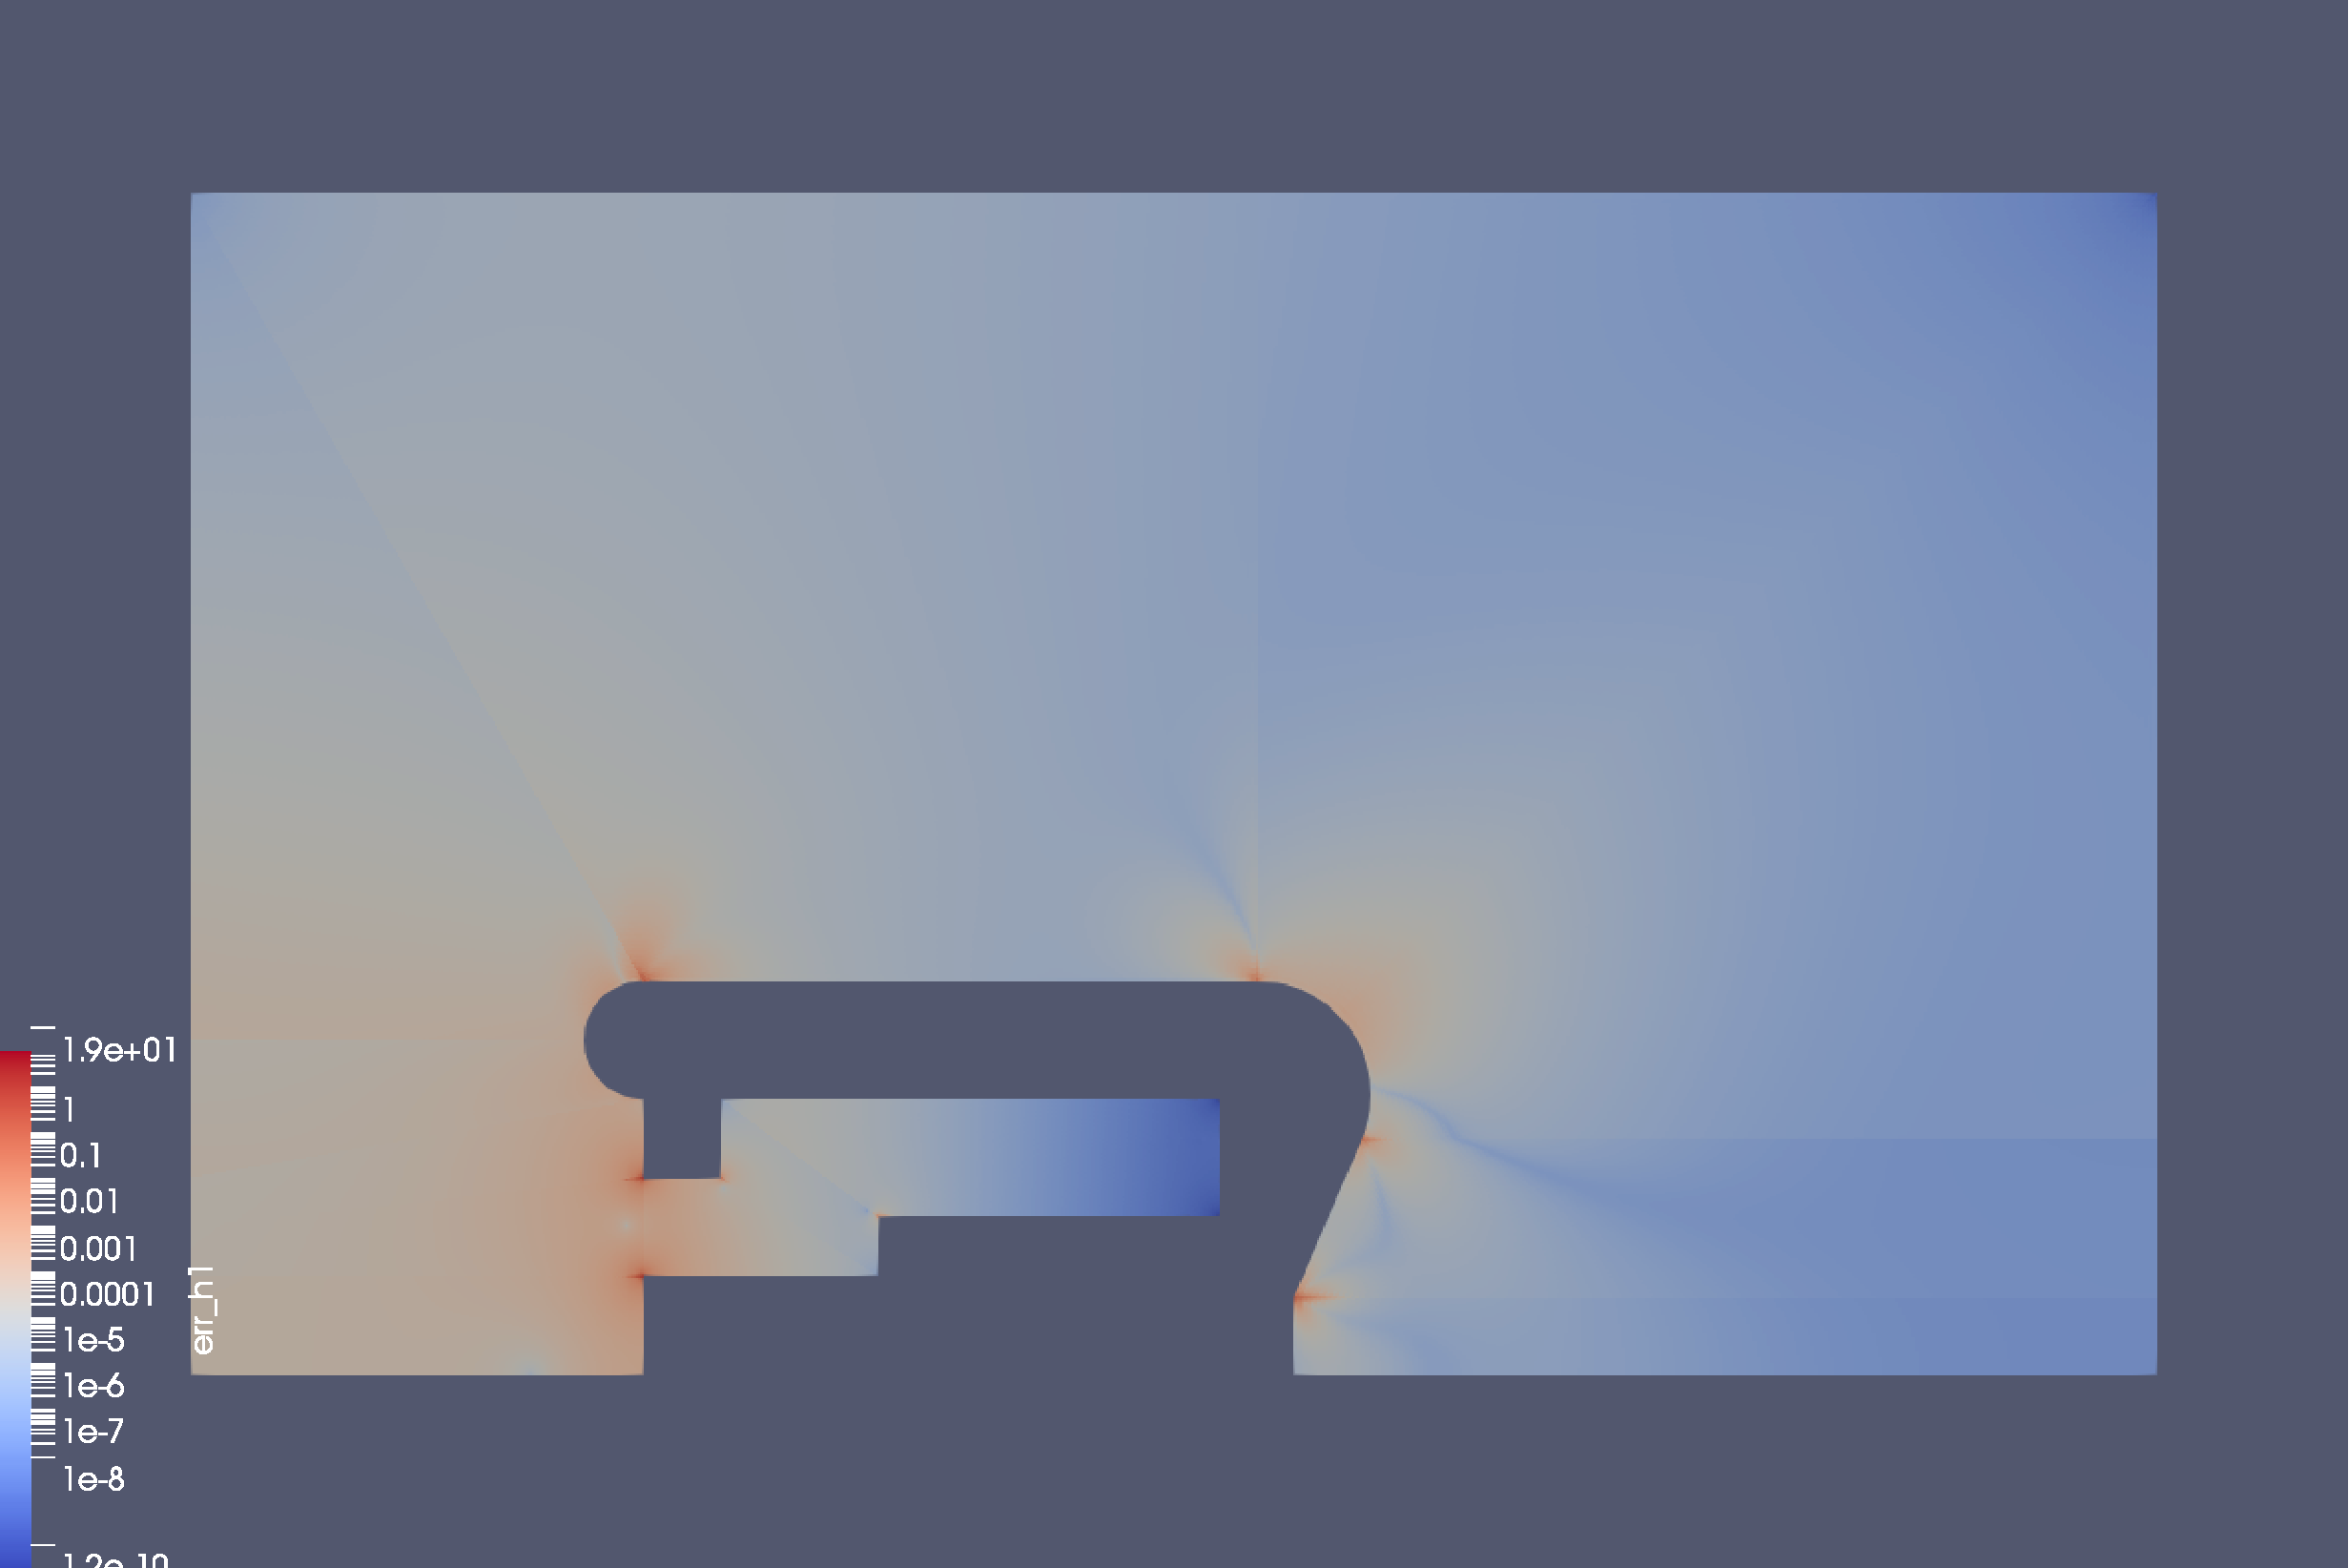
\includegraphics[width=\textwidth]{figures/insulator/error_elem}
  \caption{Absolute error of the electric field on every element.}
  \label{fig:error_elem}
\end{figure}
\end{center}
